\documentclass[10pt]{article}
\usepackage[utf8]{inputenc}
\usepackage[T1]{fontenc}
\usepackage{amsmath}
\usepackage{amsfonts}
\usepackage{amssymb}
\usepackage[version=4]{mhchem}
\usepackage{stmaryrd}
\usepackage{graphicx}
\usepackage[export]{adjustbox}
\graphicspath{ {./images/} }
\usepackage{bbold}
\usepackage{caption}
\usepackage{multirow}
\usepackage{fvextra, csquotes}

\newcommand\longdiv[1]{\overline{\smash{)}#1}}

%New command to display footnote whose markers will always be hidden
\let\svthefootnote\thefootnote
\newcommand\blfootnotetext[1]{%
  \let\thefootnote\relax\footnote{#1}%
  \addtocounter{footnote}{-1}%
  \let\thefootnote\svthefootnote%
}

%Overriding the \footnotetext command to hide the marker if its value is `0`
\let\svfootnotetext\footnotetext
\renewcommand\footnotetext[2][?]{%
  \if\relax#1\relax%
    \ifnum\value{footnote}=0\blfootnotetext{#2}\else\svfootnotetext{#2}\fi%
  \else%
    \if?#1\ifnum\value{footnote}=0\blfootnotetext{#2}\else\svfootnotetext{#2}\fi%
    \else\svfootnotetext[#1]{#2}\fi%
  \fi
}

\DeclareUnicodeCharacter{2234}{\ifmmode\therefore\else{$\therefore$}\fi}
\DeclareUnicodeCharacter{25A1}{\ifmmode\square\else{$\square$}\fi}
\DeclareUnicodeCharacter{2713}{\ifmmode\checkmark\else{$\checkmark$}\fi}

\begin{document}
\captionsetup{singlelinecheck=false}
Gina correctly started to answer the following question. Complete her solution.\\
Question: Solve the following equation for all real values of $\theta$.\\
Express your answer in radians correct to 3 decimal places.

$$
3 \sin ^{2} \theta-14 \sin \theta-5=0
$$

Gina's solution: $3 \sin ^{2} \theta-14 \sin \theta-5=0$

$$
(3 \sin \theta+1)(\sin \theta-5)=0
$$

\section*{Solution}
\section*{Method 1}
$$
\begin{array}{r}
3 \sin ^{2} \theta-14 \sin \theta-5=0 \\
(3 \sin \theta+1)(\sin \theta-5)=0
\end{array}
$$

$$
\begin{array}{lll}
\sin \theta=-\frac{1}{3} & \sin \theta=5 & 1 / 2 \text { mark for } \sin \theta=5 \\
\text { no solution } & 1 / 2 \text { mark for no solution }
\end{array}
$$

$$
\theta_{r}=0.339837
$$

$$
\theta=3.481429,5.943348 \quad 1 \text { mark }\left(\frac{1}{2} \text { mark for each value of } \theta\right)
$$

$$
\begin{aligned}
& \theta=3.481+2 k \pi, k \in \mathrm{I} \\
& \theta=5.943+2 k \pi, k \in \mathrm{I}
\end{aligned}
$$

1 mark for general solution

\section*{3 marks}
Note(s):

\begin{itemize}
  \item give maximum of 2 marks for solution in degrees: $\theta=199.471^{\circ}+360^{\circ} k, k \in \mathrm{I}$
\end{itemize}

$$
\theta=340.529^{\circ}+360^{\circ} k, k \in \mathrm{I}
$$

\section*{Method 2}
$$
y=3 \sin ^{2} \theta-14 \sin \theta-5
$$

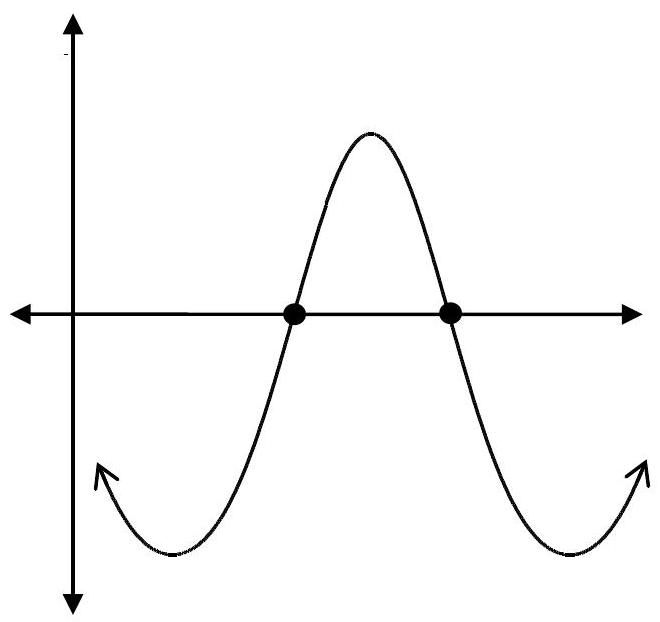
\includegraphics[max width=\textwidth, alt={}, center]{f67fedaf-ea11-42ad-a16e-f30d2fcf2bd3-002_622_660_603_207}\\
or\\
Find all zeros over the reals.

$$
\theta=3.481+2 k \pi, k \in \mathrm{I}
$$

$\theta=5.943+2 k \pi, k \in \mathrm{I}$

$$
\frac{1}{2} \text { mark for equation }
$$

$\frac{1}{2}$ mark for justification

\section*{1 mark for solutions}
1 mark for general solution\\
3 marks

Find and simplify the 6 th term in the binomial expansion of $\left(3 x^{4}-\frac{1}{x^{3}}\right)^{9}$.

\section*{Solution}
$$
\begin{array}{rlr}
t_{6} & ={ }_{9} C_{5}\left(3 x^{4}\right)^{4}\left(-\frac{1}{x^{3}}\right)^{5} & 2 \text { marks (1 mark for }{ }_{9} C_{5}, 1 / 2 \text { mark for each consistent factor) } \\
& =(126)\left(81 x^{16}\right)\left(-\frac{1}{x^{15}}\right) & \\
& =-10206 x & \begin{array}{l}
1 \text { mark for simplification }(1 / 2 \text { mark for evaluating coefficient, } 1 / 2 \text { mark } \\
\text { for simplifying variable })
\end{array}
\end{array}
$$

The number of times a website is visited can be modeled by the function:

$$
A=800(e)^{r t}
$$

where $A=$ the total number of visitors at time $t$\\
$t=$ the time in days $(t \geq 0)$\\
$r=$ the rate of growth\\
After 5 days, 40000 people have visited the site.\\
Determine the number of visitors expected after 9 days.\\
Express your answer as a whole number.

\section*{Solution}
\section*{Method 1}
$40000=800 e^{r 5}$\\
$\frac{1}{2}$ mark for substitution

$$
\begin{array}{rlr}
\frac{40000}{800} & =e^{5 r} & \\
\ln 50 & =\ln e^{5 r} & 1 / 2 \text { mark for applying logs } \\
\ln 50 & =5 r & 1 \text { mark for log theorem } \\
\frac{\ln 50}{5} & =r & \\
r & =0.782404601 &
\end{array}
$$

$$
\begin{aligned}
& A=800 e^{(0.782404601)(9)} \\
& A=914610.103 \\
& A=914610
\end{aligned}
$$

$\frac{1}{2}$ mark for substitution\\
$\frac{1}{2}$ mark for calculations with base $e$\\
3 marks

\section*{Method 2}
Use calculator to find the value of $r$.\\
$y=40000$\\
$y=800 e^{5 x}$\\
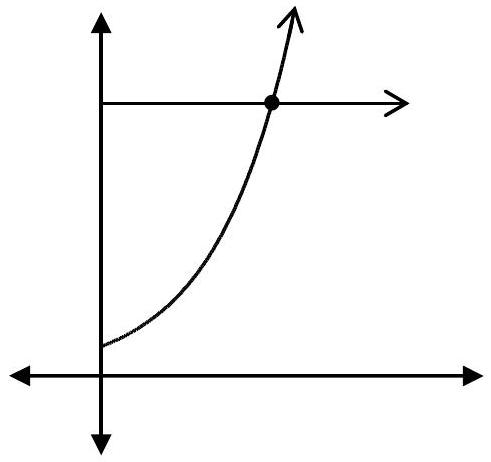
\includegraphics[max width=\textwidth, alt={}, center]{f67fedaf-ea11-42ad-a16e-f30d2fcf2bd3-005_462_491_898_191}\\
or\\
Find the point of intersection of these two functions.

$$
x=0.782404601
$$

Substitute $x$ for $r$ into formula.

$$
\begin{aligned}
\therefore A & =800 e^{(0.782404601)(9)} \\
A & =914610.103 \\
A & =914610
\end{aligned}
$$

$\frac{1}{2}$ mark for equations\\
$\frac{1}{2}$ mark for justification

1 mark for finding the value of $x$ at the intersection point

1 mark for value of $A$

3 marks

Solve algebraically:

$$
10^{3 x}=7^{x+5}
$$

Express your answer correct to 3 decimal places.

\section*{Solution}
\section*{Method 1}
$$
\begin{array}{rlrl}
10^{3 x} & =7^{x+5} & \\
\log 10^{3 x} & =\log 7^{x+5} & 1 / 2 \text { mark for applying logs } \\
3 x(\log 10) & =(x+5) \log 7 & 1 \text { mark for power rule } & \\
3 x \log 10 & =x \log 7+5 \log 7 & & \\
3 x \log 10-x \log 7 & =5 \log 7 & 1 / 2 \text { mark for collecting terms with } x & \\
x & =\frac{5 \log 7}{3 \log 10-\log 7} & 1 / 2 \text { mark for solving for } x \\
x & =1.960873 & 1 / 2 \text { mark for evaluating quotient of } \\
x & =1.961 & & \text { logarithms }
\end{array}
$$

\section*{Method 2}
$$
\begin{aligned}
10^{3 x} & =7^{x+5} \\
\log 10^{3 x} & =\log 7^{x+5} \\
3 x(\log 10) & =(x+5) \log 7 \\
3 x & =x \log 7+5 \log 7
\end{aligned}
$$

$3 x-x \log 7=5 \log 7$

$$
\begin{aligned}
& x=\frac{5 \log 7}{3-\log 7} \\
& x=1.960873 \\
& x=1.961
\end{aligned}
$$

A word contains two Ms, two Es, two Ns, and no other repeated letters.\\
Suppose one of the Ns is replaced by an M.\\
Will this replacement result in greater or fewer permutations?\\
Justify your reasoning.

\section*{Solution}
\section*{Method 1}
$2 \mathrm{Ms}, 2 \mathrm{Es}, 2 \mathrm{Ns}: \frac{(\text { total number of letters })!}{2!2!2!}$ 1 mark for dividing the total number of letters by $2!2!2!$

$$
\frac{(\text { total number of letters })!}{8}
$$

$3 \mathrm{Ms}, 2 \mathrm{Es}, 1 \mathrm{~N}$ : $\frac{\text { (total number of letters)! }}{3!2!1!}$ 1 mark for dividing the total number of letters by $3!2!1!$

$$
\frac{(\text { total number of letters })!}{12}
$$

If one of the Ns is changed to an M, there would be fewer permutations.

\section*{Method 2}
If one of the Ns is changed to an M, there would be fewer permutations because you would be dividing the total number of letters by a larger number.

2 marks for justification\\
2 marks

There is a group of 16 boys and 12 girls. How many ways can a committee of 3 people be formed if there must be at least 2 girls on the committee?\\
Express your answer as a whole number.

\section*{Solution}
\section*{Method 1}
Case 1: 2 girls, 1 boy\\
Case 2: 3 girls

$$
{ }_{12} C_{2} \cdot{ }_{16} C_{1}=1056
$$

$$
{ }_{12} C_{3}=220
$$

$$
1056+220=1276
$$

1 mark for case 1 ( $\frac{1}{2}$ mark for each factor shown in a product)\\
1 mark for case 2\\
1 mark for addition of cases\\
3 marks

\section*{Method 2}
Case 1: 2 boys, 1 girl\\
Case 2: 3 boys\\
All possibilities\\
${ }_{16} C_{2} \cdot{ }_{12} C_{1}=1440$

$$
{ }_{16} C_{3}=560
$$

${ }_{28} C_{3}=3276$\\
$3276-1440-560=1276$

1 mark for case 1 ( $\frac{1}{2}$ mark for each factor shown in a product)\\
1 mark for case 2\\
$\frac{1}{2}$ mark for all possible cases\\
$\frac{1}{2}$ mark for subtraction from total\\
3 marks

A student is using the formula $s=\theta r$ to find an arc length of a circle. Given a central angle measure of $35^{\circ}$ and a radius of 6 cm , the student's solution is as follows:

$$
\begin{aligned}
& s=(35)(6) \\
& s=210 \mathrm{~cm}
\end{aligned}
$$

Explain why this solution is incorrect.\\
Write the correct solution.

\section*{Solution}
When using the formula $s=\theta r$, the angle must be in radians. $\frac{1}{2}$ mark for explanation\\
$35^{\circ}\left(\frac{\pi}{180^{\circ}}\right)=\frac{35 \pi}{180} \quad$ or $\quad \frac{7 \pi}{36}$\\
$\therefore s=\theta r$

$$
\begin{aligned}
& =\frac{7 \pi}{36}(6) \\
& =\frac{42 \pi}{36} \mathrm{~cm} \quad \text { or } \quad \frac{7 \pi}{6} \mathrm{~cm} \quad \text { or } \quad 3.665 \mathrm{~cm}
\end{aligned}
$$

1 mark for conversion to radians

$$
\frac{1}{2} \text { mark for simplification }
$$

2 marks

Note(s):

\begin{itemize}
  \item award 1 mark for correct final answer with no work
\end{itemize}

Given the graph of $f(x)$ below, explain how you would sketch the graph of $y=|f(x)|$.\\
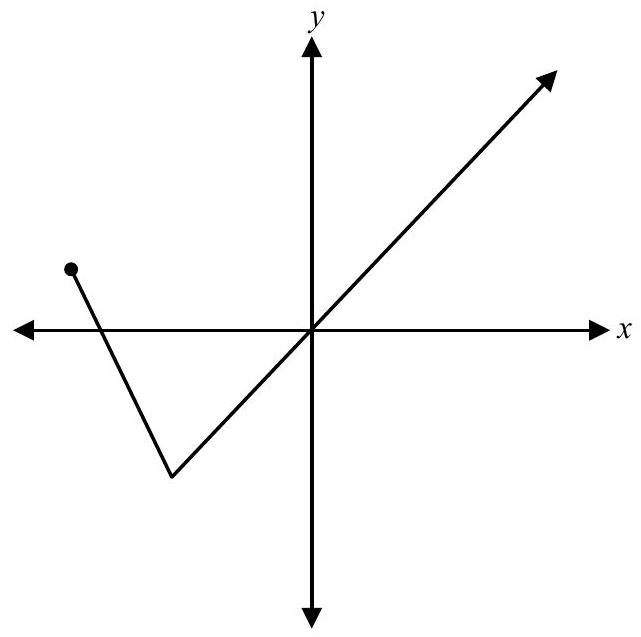
\includegraphics[max width=\textwidth, alt={}, center]{f67fedaf-ea11-42ad-a16e-f30d2fcf2bd3-010_637_641_476_249}

\section*{Solution}
The negative $y$ values are reflected over the $x$-axis.

1 mark for explanation\\
1 mark

Claire correctly solves the following equation:

$$
\log _{2}(6-x)+\log _{2}(3-x)=2
$$

She finds two possible values of $x$ : $x=2$ and $x=7$.\\
Identify which one of these values is unacceptable and explain why.

\section*{Solution}
If $x$ is greater than 3 , you have a negative argument $\therefore x=2$ but $x \neq 7$.\\
or\\
The domain is restricted to values of $x<3 \therefore x=2$.

1 mark for explanation\\
1 mark

Given the graph of the function $f(x)$ below, state the domain of $y=\sqrt{f(x)}$.\\
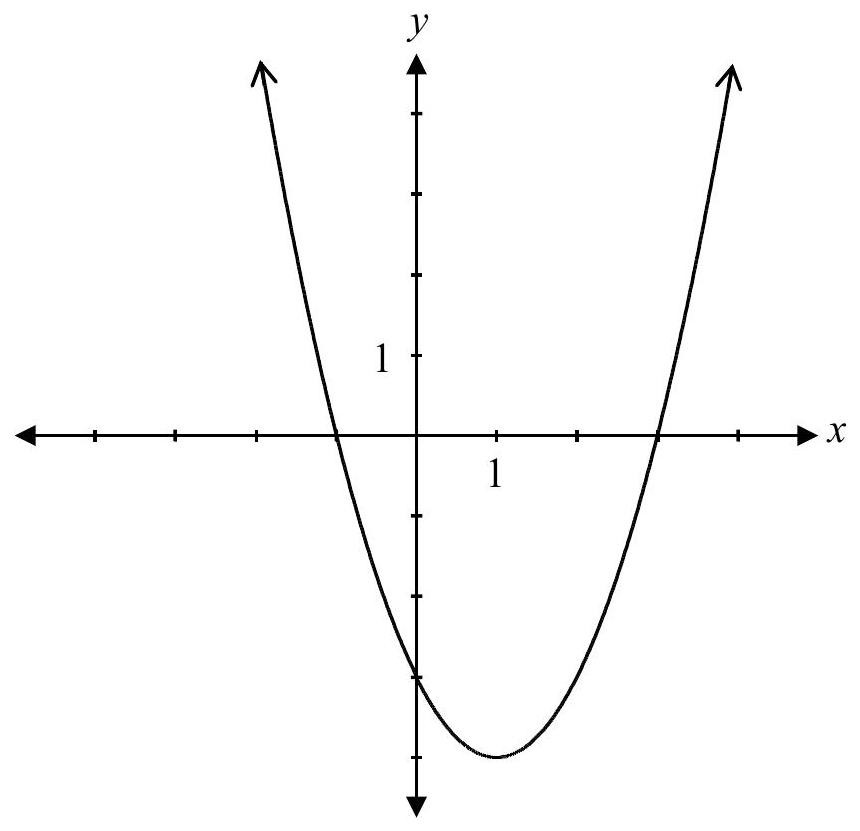
\includegraphics[max width=\textwidth, alt={}, center]{f67fedaf-ea11-42ad-a16e-f30d2fcf2bd3-012_831_860_517_234}

\section*{Solution}
The domain is $\{x \in \mathbb{R} \mid x \leq-1$ or $x \geq 3\}$.\\
or

1 mark for domain\\
1 mark

The domain is $(-\infty,-1] \cup[3, \infty)$.

A school offers 4 different Science courses, 3 different Mathematics courses, and 2 different English courses.

Julie must select 1 Science course, 1 Mathematics course, and 1 English course. She thinks this creates 9 options for her timetable.

Show why Julie is incorrect.

\section*{Solution}
Julie should have multiplied the number of options.\\
or\\
$4 \times 3 \times 2=24$ different options

1 mark for justification\\
1 mark

Explain how Pascal's triangle can be used to determine the coefficients in the binomial expansion of $(x+y)^{n}$.

\section*{Solution}
The $(n+1)^{\text {st }}$ row of Pascal's triangle corresponds to the coefficients of the terms in the expansion of the binomial $(x+y)^{n}$.

1 mark for explanation\\
1 mark

Prove the identity below for all permissible values of $x$ :

$$
\frac{1+\cos 2 x}{\sin 2 x}=\cot x
$$

\section*{Solution}
\section*{Method 1}
$$
\begin{aligned}
\text { LHS } & =\frac{1+2 \cos ^{2} x-1}{2 \sin x \cos x} \\
& =\frac{2 \cos ^{2} x}{2 \sin x \cos x} \\
& =\frac{\cos x}{\sin x} \\
& =\cot x \\
& =\text { RHS }
\end{aligned}
$$

1 mark for identity\\
$\frac{1}{2}$ mark for identity\\
1 mark for simplification\\
$\frac{1}{2}$ mark for identity\\
3 marks

\section*{Method 2}
$$
\begin{array}{rlr}
\text { LHS } & =\frac{1+1-2 \sin ^{2} x}{2 \sin x \cos x} & \\
& =\frac{1 / 2 \text { mark for identity }}{2 \sin x \cos x} & \\
& =\frac{1-\sin ^{2} x}{\sin x \cos x} & \\
& =\frac{\cos ^{2} x}{\sin x \cos x} & \\
& =\frac{\cos x}{\sin x} \text { mark for simplification } \\
& =\cot x & \\
& =\text { RHS } & 1 / 2 \text { mark for identity } \\
& 1 / 2 \text { mark for simplification } \\
& \mathbf{3} \text { marks for identity }
\end{array}
$$

\section*{Solution}
\section*{Method 3}
$$
\begin{aligned}
\text { LHS } & =\frac{1+\cos ^{2} x-\sin ^{2} x}{2 \sin x \cos x} \\
& =\frac{2 \cos ^{2} x}{2 \sin x \cos x} \\
& =\frac{\cos x}{\sin x} \\
& =\cot x \\
& =\text { RHS }
\end{aligned}
$$

$\frac{1}{2}$ mark for identity\\
$\frac{1}{2}$ mark for identity\\
$\frac{1}{2}$ mark for identity $\left(1-\sin ^{2} x=\cos ^{2} x\right)$\\
1 mark for simplification\\
$\frac{1}{2}$ mark for identity\\
3 marks

Your classmate, Leo, was absent for one of his math lessons.\\
Explain to Leo how to determine the cosecant ratio for an angle in standard position given that $\mathrm{P}(-3,-4)$ is a point on the terminal arm of the angle.

\section*{Solution}
\section*{Method 1}
\begin{itemize}
  \item Locate the point $(-3,-4)$ on the coordinate plane.
  \item Draw a right-angle triangle by connecting the point $(-3,-4)$ to the $x$-axis and to the origin.
  \item The angle created with the $x$-axis and the line connecting the point with the origin (the terminal arm) is $\theta$.
  \item Determine the length of the terminal arm by using the Pythagorean Theorem.
  \item Once you have the lengths of all three sides of the triangle, find $\sin \theta$.
  \item Invert the $\sin \theta$ ratio to find $\csc \theta$.
\end{itemize}

\section*{Method 2}
\begin{itemize}
  \item Determine the value of $r$ using the Pythagorean Theorem.\\
$\frac{1}{2}$ mark
  \item Determine the value of $\sin \theta\left(\sin \theta=\frac{y}{r}\right)$.
  \item Identify the correct quadrant.
  \item Invert the $\sin \theta$ ratio to find $\csc \theta$. $\frac{1}{2}$ mark $\frac{1}{2}$ mark $\frac{1}{2}$ mark 2 marks
\end{itemize}

Note(s):

\begin{itemize}
  \item award a maximum of 1 mark for correct work shown without an explanation in words
\end{itemize}

Given the following graphs:

$$
f(x)
$$

\begin{center}
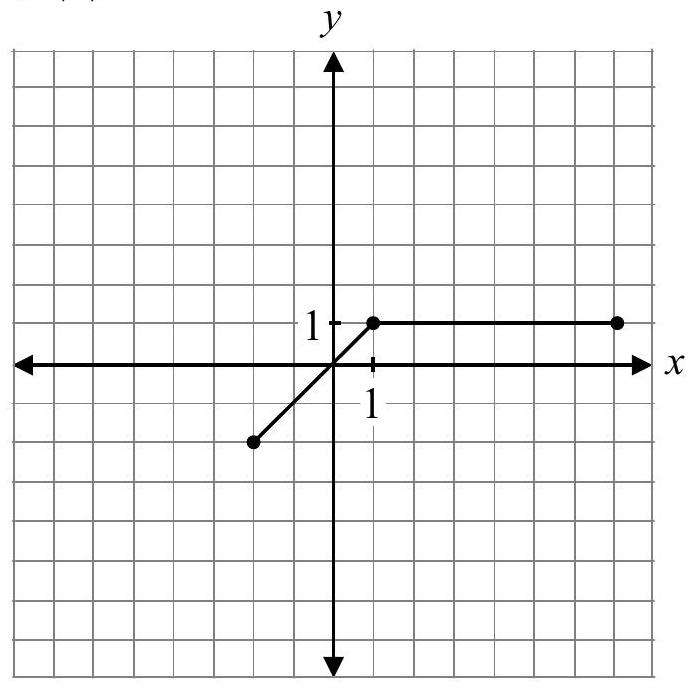
\includegraphics[max width=\textwidth, alt={}]{f67fedaf-ea11-42ad-a16e-f30d2fcf2bd3-018_688_695_526_298}
\end{center}

\begin{figure}[h]
\begin{center}
\captionsetup{labelformat=empty}
\caption{$g(x)$}
  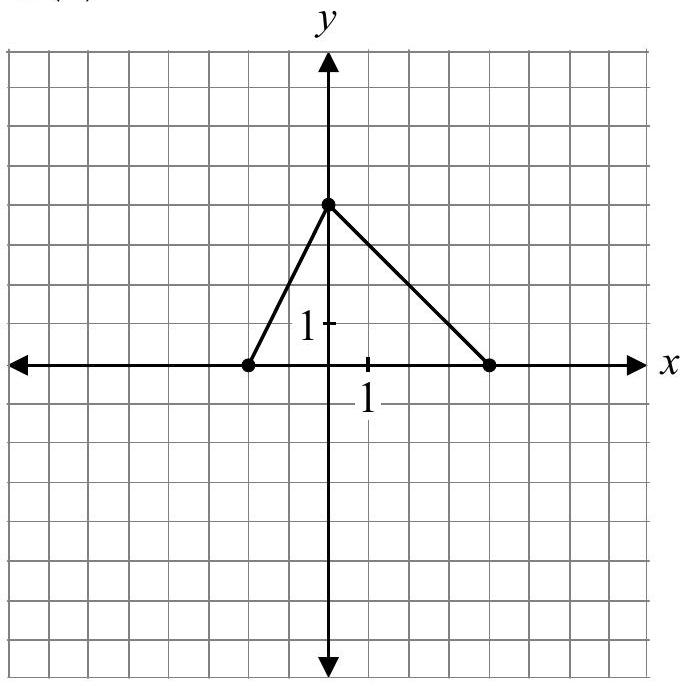
\includegraphics[alt={},max width=\textwidth]{f67fedaf-ea11-42ad-a16e-f30d2fcf2bd3-018_686_691_526_1168}
\end{center}
\end{figure}

Sketch the graph of $f(x)+g(x)$.

\section*{Solution}
\begin{center}
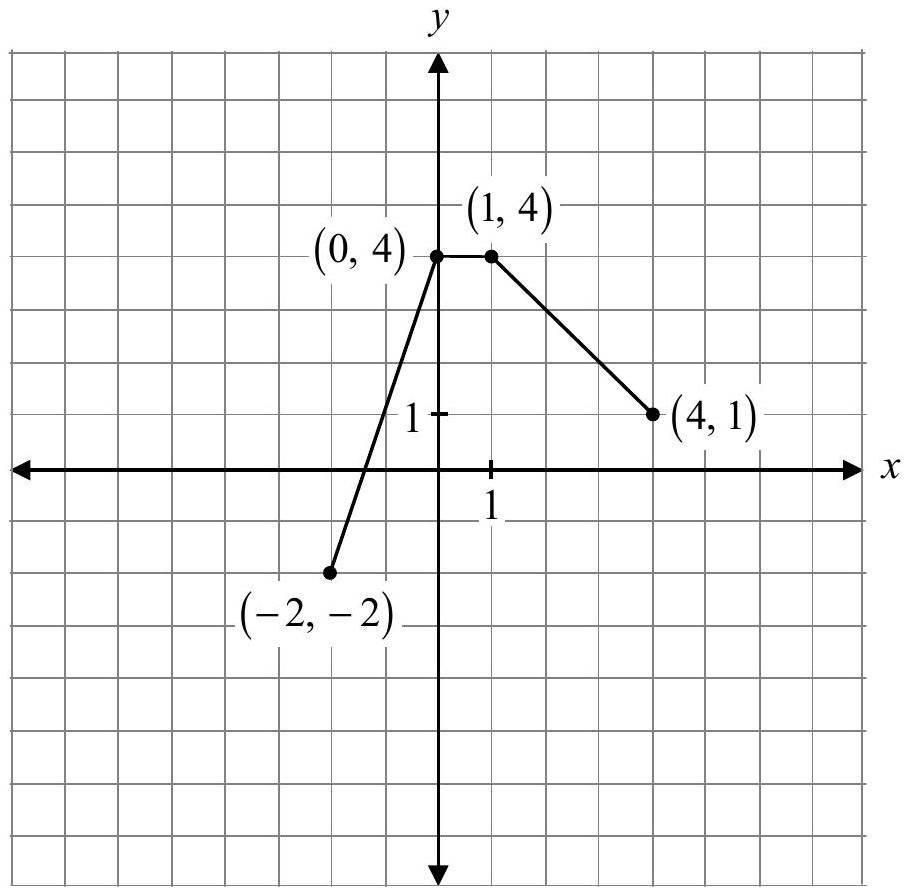
\includegraphics[max width=\textwidth, alt={}]{f67fedaf-ea11-42ad-a16e-f30d2fcf2bd3-018_894_912_1433_249}
\end{center}

2 marks ( $\frac{1}{2}$ mark for each point where the graph changes direction)

$$
[(-2,-2) ;(0,4) ;(1,4) ;(4,1)]
$$

\begin{center}

\includegraphics[max width=\textwidth, alt={}]{f67fedaf-ea11-42ad-a16e-f30d2fcf2bd3-018_135_234_1703_1179}
\end{center}

Note(s):

\begin{itemize}
  \item deduct a maximum of 1 mark for incorrect domain
\end{itemize}

If $(2,3)$ is a point on the graph of $y=f(x)$, what point must be on the graph of $y=3 f\left(\frac{1}{4} x\right)$ ?\\
a) $\left(\frac{1}{2}, 1\right)$\\
b) $\left(\frac{1}{2}, 9\right)$\\
c) $(8,1)$\\
d) $(8,9)$

\section*{Question 17}
Consider the arc drawn on each circle. Which arc measure is closest to 3 radians?

\begin{figure}[h]
\begin{center}
\captionsetup{labelformat=empty}
\caption{a)}
  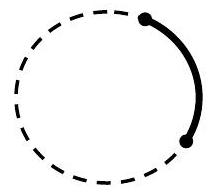
\includegraphics[alt={},max width=\textwidth]{f67fedaf-ea11-42ad-a16e-f30d2fcf2bd3-019_193_211_1301_234}
\end{center}
\end{figure}

\begin{figure}[h]
\begin{center}
\captionsetup{labelformat=empty}
\caption{b)}
  
\includegraphics[alt={},max width=\textwidth]{f67fedaf-ea11-42ad-a16e-f30d2fcf2bd3-019_130_133_1330_671}
\end{center}
\end{figure}

\begin{figure}[h]
\begin{center}
\captionsetup{labelformat=empty}
\caption{c)}
  
\includegraphics[alt={},max width=\textwidth]{f67fedaf-ea11-42ad-a16e-f30d2fcf2bd3-019_223_227_1284_1123}
\end{center}
\end{figure}

\begin{figure}[h]
\begin{center}
\captionsetup{labelformat=empty}
\caption{d)}
  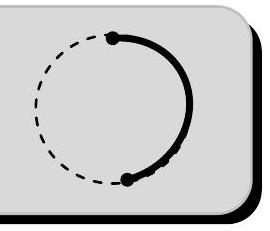
\includegraphics[alt={},max width=\textwidth]{f67fedaf-ea11-42ad-a16e-f30d2fcf2bd3-019_231_270_1284_1546}
\end{center}
\end{figure}

\section*{Question 18}
If $\log _{2} x=4$, then $\log _{2}(2 x)$ is equal to:\\
a) 5\\
b) 8\\
c) 16\\
d) 32

Simplify the following expression:

$$
\cos ^{2} x\left(1+\cot ^{2} x\right)
$$

a) $\sin ^{2} x$\\
b) $\cos ^{2} x$\\
c) $\cot ^{2} x$\\
d) $\sec ^{2} x$

Question 20

Identify the graph of the function $y=\frac{x}{x}$.\\
a)\\
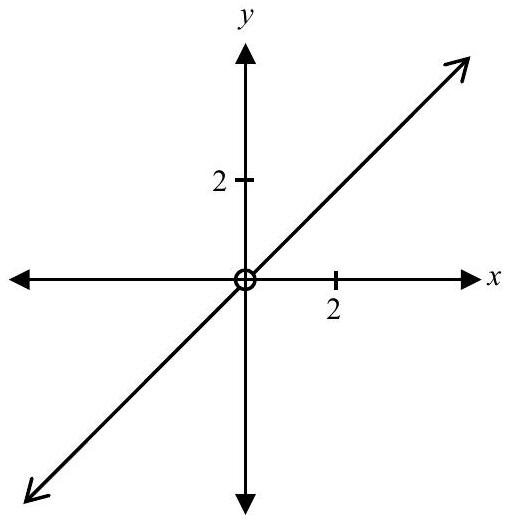
\includegraphics[max width=\textwidth, alt={}, center]{f67fedaf-ea11-42ad-a16e-f30d2fcf2bd3-020_523_514_1173_322}\\
b)\\
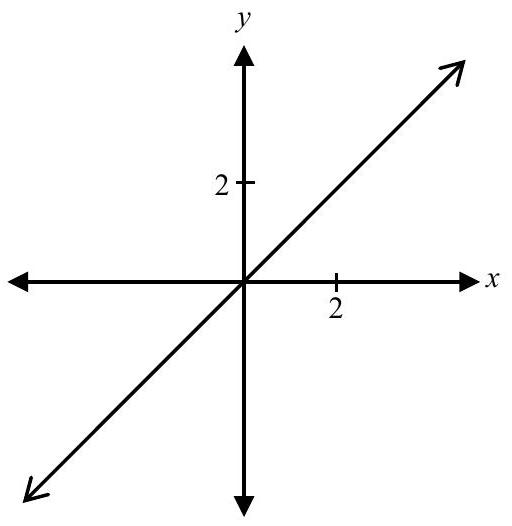
\includegraphics[max width=\textwidth, alt={}, center]{f67fedaf-ea11-42ad-a16e-f30d2fcf2bd3-020_526_512_1112_1173}\\
c)\\
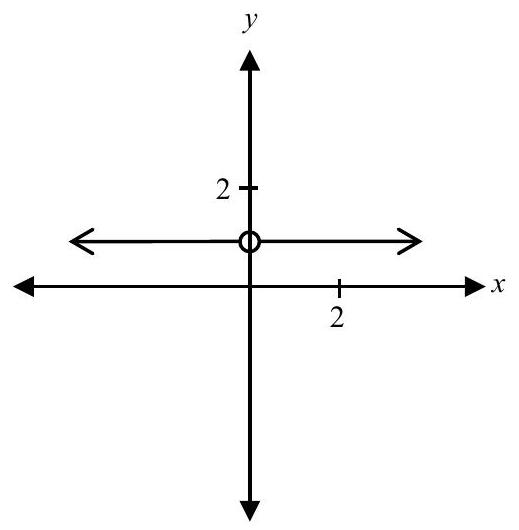
\includegraphics[max width=\textwidth, alt={}, center]{f67fedaf-ea11-42ad-a16e-f30d2fcf2bd3-020_530_519_1789_317}\\
d)\\
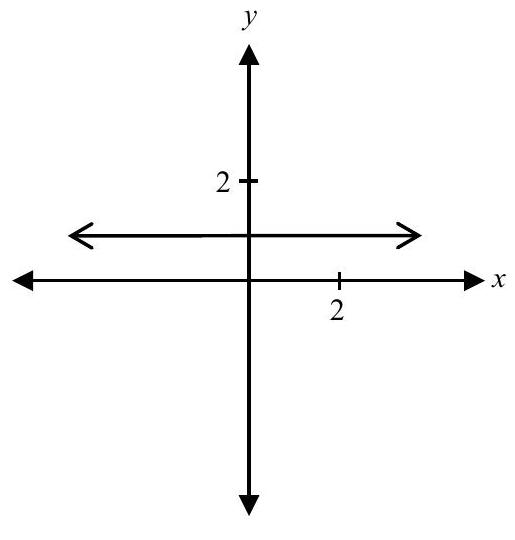
\includegraphics[max width=\textwidth, alt={}, center]{f67fedaf-ea11-42ad-a16e-f30d2fcf2bd3-020_540_515_1774_1181}

How many terms are in the expansion of $\left(3 y^{2}-4 z\right)^{7}$ ?\\
a) 2\\
b) 6\\
c) 7\\
d) 8

Question 22\\
R6

Determine one possible restriction for the domain of $y=(x+3)^{2}-4$ so that its inverse is a function.\\
a) $x \leq-3$\\
b) $x \leq 0$\\
c) $x \leq 3$\\
d) $x \leq 4$

Question 23

Find the total possible number of arrangements for 7 adults and 3 children seated in a row if the 3 children must sit together.\\
a) 10 !\\
b) $8!3!$\\
c) $7!3!$\\
d) 7 !

Question 24

Identify the value of the $x$-intercept of the function $y=\ln (x-2)$.\\
a) -1\\
b) 0\\
c) 2\\
d) 3

Given $\log _{b} a=3$, give one example of possible values for $a$ and $b$ that make this equation true.

\section*{Solution}
Answers will vary but $b^{3}=a$.\\
Some possible solutions are: $a=8 \quad b=2$\\
or

$$
a=27 \quad b=3
$$

or

$$
a=64 \quad b=4
$$

\section*{Question 26}
The range of the graph of $y=f(x)$ is $[-3,2]$.\\
Explain why there is no effect on the range of the graph that is a result of the transformation $y=f(-x)$.

\section*{Solution}
$y=f(-x)$ is a reflection over the $y$-axis.\\
The domain is affected, but the range remains the same.

1 mark for explanation\\
1 mark

Sketch the graph of $y=(x+1)(x-2)^{2}(x+5)$.\\
Identify the $x$-intercepts and $y$-intercept.

\section*{Solution}
$x$-intercepts: $-5,-1$, and 2\\
$y$-intercept: 20\\
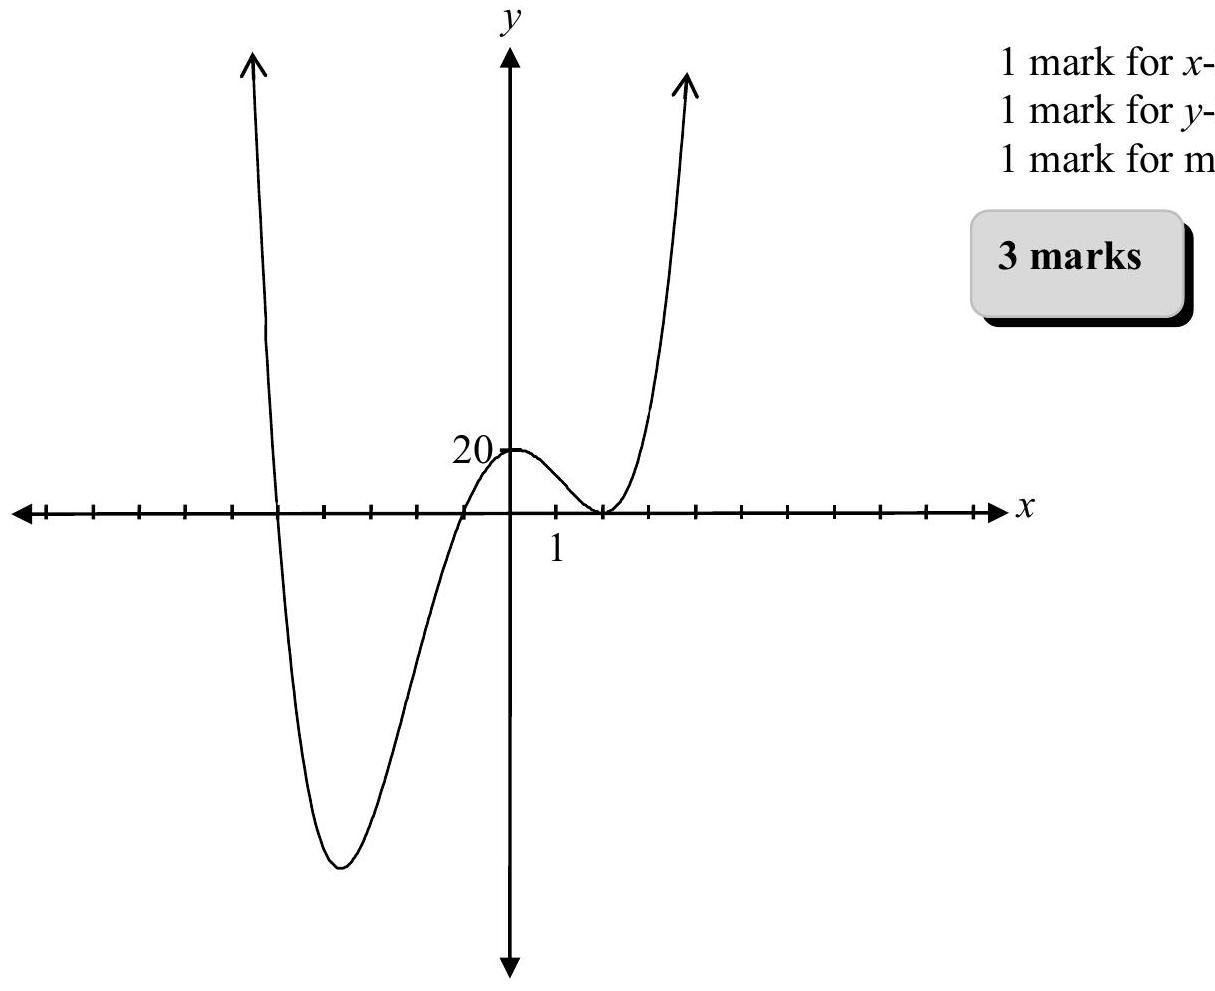
\includegraphics[max width=\textwidth, alt={}, center]{f67fedaf-ea11-42ad-a16e-f30d2fcf2bd3-023_991_1215_859_210}

Note(s):

\begin{itemize}
  \item if no graph is shown, give $\frac{1}{2}$ mark for $x$-intercepts $\left(-5,-1\right.$, and 2 ) and $\frac{1}{2}$ mark for $y$-intercept (20)
  \item relative maximum and minimum are not required
\end{itemize}

The graph of the function $y=\sin x$ has been transformed to create a new graph.\\
The range of this new graph is $[-4,4]$ and the zeros are $x=k \frac{\pi}{2}$, where $k$ is an integer.\\
Write the equation that corresponds to this new graph.

\section*{Solution}
$$
\begin{aligned}
\text { Amplitude } & =4 & & 1 \text { mark for correct amplitude } \\
\text { Period } & =\pi & & 1 / 2 \text { mark for correct period } \\
\therefore b & =\frac{2 \pi}{\pi}=2 & & 1 / 2 \text { mark for consistent value of } b \\
y & =4 \sin (2 x) & & \mathbf{2} \text { marks }
\end{aligned}
$$

or

Note(s):

\begin{itemize}
  \item deduct $\frac{1}{2}$ mark for a translation that results in an incorrect range and/or zeros
\end{itemize}

Question 29

Given the functions $f(x)=x^{2}-1$ and $g(x)=x+1$, state the domain of $\frac{g(x)}{f(x)}$.

\section*{Solution}
Domain: $x \in \mathbb{R}$ where $x \neq 1$ and $x \neq-1$ 1 mark ( $\frac{1}{2}$ mark for $x \neq 1, \frac{1}{2}$ mark for $x \neq-1$ )\\
a) Sketch the graph of $y=3^{x}$.\\
b) Explain how the graph of $y=3^{x}$ can be used to sketch the graph of $y=\log _{3} x$.

\section*{Solutions}
a)\\
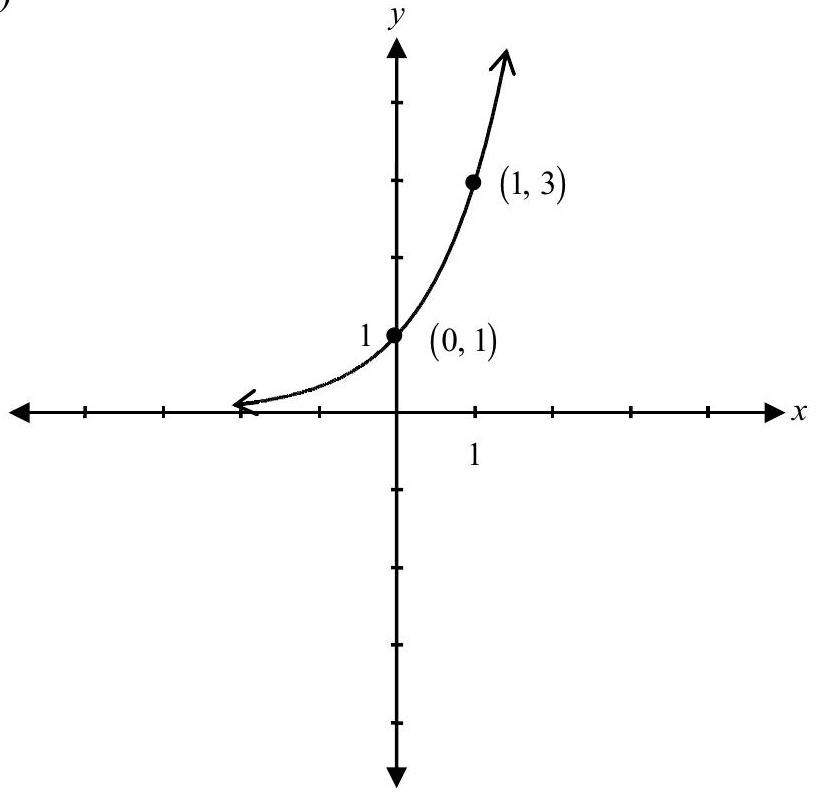
\includegraphics[max width=\textwidth, alt={}, center]{f67fedaf-ea11-42ad-a16e-f30d2fcf2bd3-025_796_816_708_214}\\
$\frac{1}{2}$ mark for increasing exponential function\\
$\frac{1}{2}$ mark for $y$-intercept at $(0,1)$\\
$\frac{1}{2}$ mark for consistent point on exponential function\\
$\frac{1}{2}$ mark for asymptotic behaviour\\
2 marks\\
b)

To graph $y=\log _{3} x$, you can reflect the graph of $y=3^{x}$ over the line $y=x$.\\
or\\
You can switch the $x$ and $y$ coordinates of $y=3^{x}$ to get the graph of $y=\log _{3} x$.

1 mark for explanation\\
1 mark

Note(s):

\begin{itemize}
  \item in (b), give $\frac{1}{2}$ mark for having only stated they are inverse functions of each other
\end{itemize}

A box in the shape of a rectangular prism has side lengths $x, x+2$, and $x+10$.\\
Write a function, $V(x)$, to express the volume of the box in terms of $x$.\\
Find all possible values of $x$, given that the volume of the box is $96 \mathrm{~cm}^{3}$.\\
State the dimensions of the box.

\section*{Solution}
$$
\begin{array}{rlrl}
V(x) & =(x)(x+2)(x+10) & 1 / 2 \text { mark for expressing volume in terms of } x \\
96 & =(x)(x+2)(x+10) & \\
96 & =x^{3}+12 x^{2}+20 x & \\
0 & =x^{3}+12 x^{2}+20 x-96 & 1 / 2 \text { mark for equating to zero }
\end{array}
$$

when $x=2$ :

$$
\begin{aligned}
& 0=(2)^{3}+12(2)^{2}+20(2)-96 \\
& 0=8+48+40-96 \\
& 0=0
\end{aligned}
$$

$\therefore x=2$ is a possible value.\\
1 mark for identifying one possible value of $x$

2 \begin{tabular}{rrrr}
1 & 12 & 20 & -96 \\
 & 2 & 28 & 96 \\
\hline
1 & 14 & 48 & 0 \\
\hline
\end{tabular}

\begin{center}
\begin{tabular}{|l|l|}
\hline
\( \begin{aligned} (x-2)\left(x^{2}+14 x+48\right) & =0 \\ (x-2)(x+8)(x+6) & =0 \\ x & =-8,-6,2 \\ x & \neq-8 \text { and } x \neq-6 \text { because dimensions } \\ & \text { cannot be negative values. } \\ \therefore x & =2 \text { is the only solution. } \end{aligned} \) & 1 mark for division \\
\hline
The dimensions of the box are $2 \mathrm{~cm} \times 4 \mathrm{~cm} \times 12 \mathrm{~cm}$. & $\frac{1}{2}$ mark for stating the dimensions of the box \\
\hline
\end{tabular}
\end{center}

Given the graph of $f(x)$ below, sketch the graph of $y=-f(x)$.\\
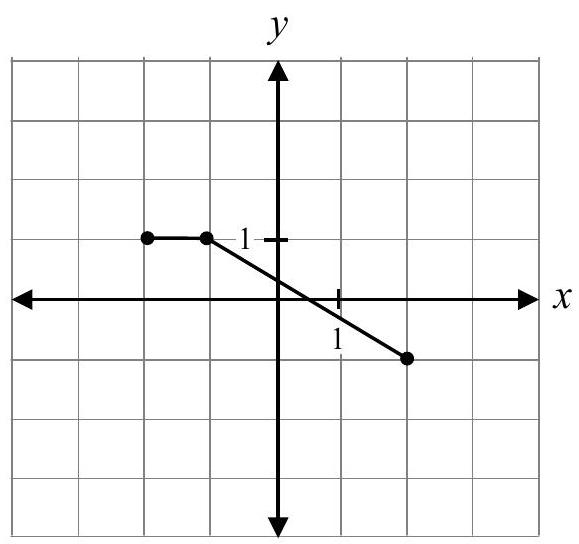
\includegraphics[max width=\textwidth, alt={}, center]{f67fedaf-ea11-42ad-a16e-f30d2fcf2bd3-027_544_579_569_259}

\section*{Solution}
\begin{center}
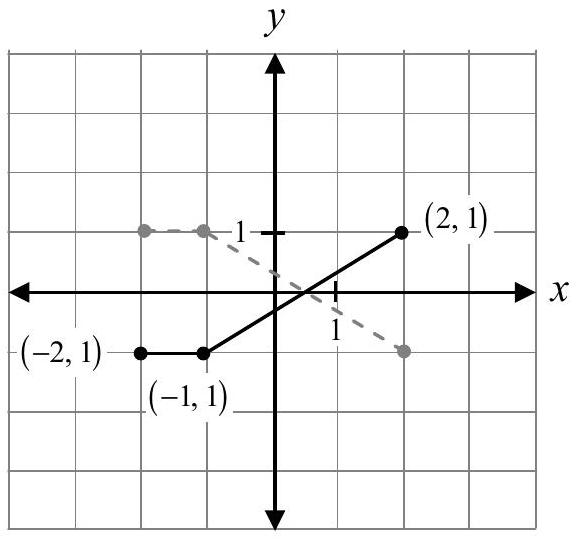
\includegraphics[max width=\textwidth, alt={}]{f67fedaf-ea11-42ad-a16e-f30d2fcf2bd3-027_540_578_567_1014}
\end{center}

Determine the coordinates of a point $(x, y)$ on the unit circle if you are given $\theta=30^{\circ}$ where $\theta$ is in standard position.

\section*{Solution}
$\mathrm{P}(\theta)=(\cos \theta, \sin \theta)$\\
If $\theta=30^{\circ}$, then the coordinates of $\mathrm{P}(\theta)$ would be $\left(\cos 30^{\circ}, \sin 30^{\circ}\right)$.

1 mark for answer stated as coordinate point\\
or\\
$\mathrm{P}\left(30^{\circ}\right)=\left(\frac{\sqrt{3}}{2}, \frac{1}{2}\right)$

Given the following sinusoidal equation:

$$
P(t)=3000 \sin \left[\frac{\pi}{10}(t-2010)\right]+10000
$$

Determine the maximum value of $\mathrm{P}(t)$ and a value of $t$ at which this maximum occurs.

\section*{Solution}
\section*{Method 1}
$$
\begin{aligned}
\text { Maximum value } & =10000+3000 & & 1 \text { mark for maximum value } \\
& =13000 & & \\
13000 & =3000 \sin \left[\frac{\pi}{10}(t-2010)\right]+10000 & & \\
3000 & =3000 \sin \left[\frac{\pi}{10}(t-2010)\right] & & 1 / 2 \text { mark for simplifying } \\
1 & =\sin \left[\frac{\pi}{10}(t-2010)\right] & & 1 \text { mark for exact value } \\
\frac{\pi}{2} & =\frac{\pi}{10}(t-2010) & & 1 / 2 \text { mark for solving for } t \\
5 & =t-2010 & & \mathbf{3} \text { marks } \\
t & =2015 & &
\end{aligned}
$$

Note(s):

\begin{itemize}
  \item the period of the function is $20 \therefore$ other acceptable answers are: $t=2015 \pm 20$
\end{itemize}

\section*{Solution}
\section*{Method 2}
\begin{center}
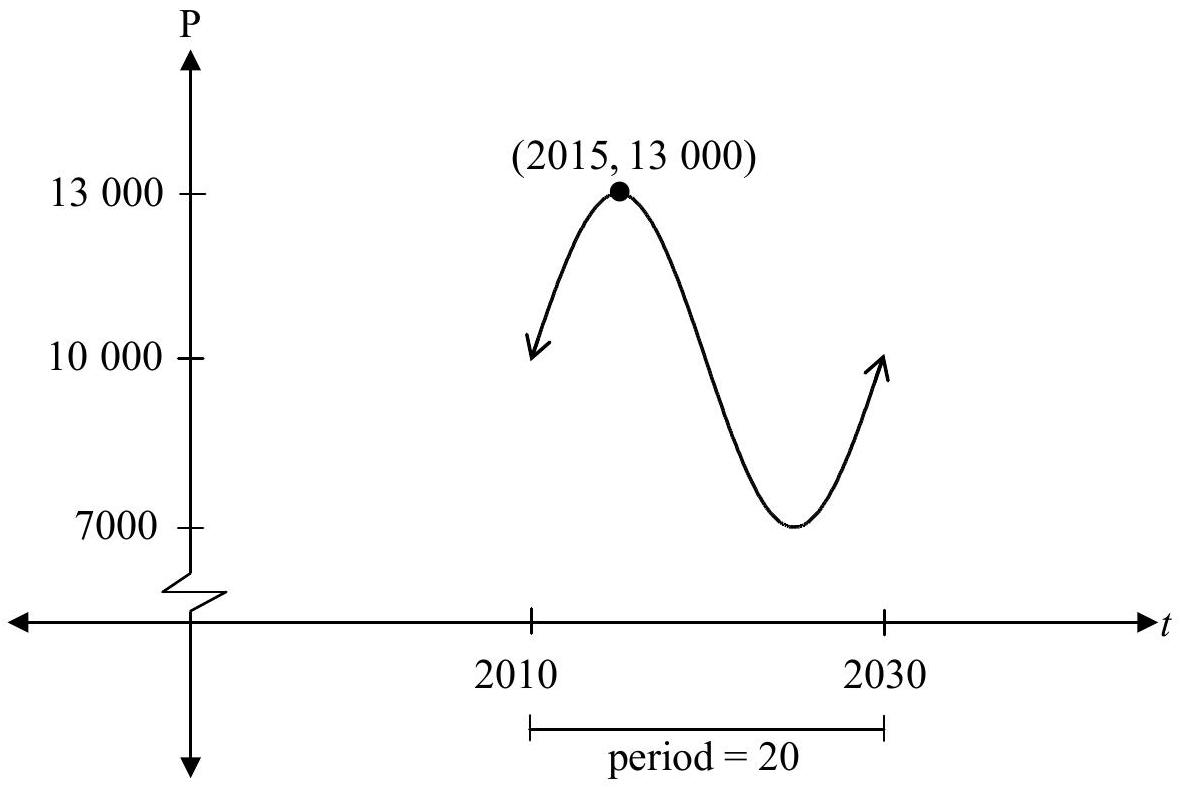
\includegraphics[max width=\textwidth, alt={}]{f67fedaf-ea11-42ad-a16e-f30d2fcf2bd3-029_787_1180_638_174}
\end{center}

1 mark for period

$$
\begin{aligned}
\mathrm{P}(t) & =13000 \\
t & =2015
\end{aligned}
$$

∴ the maximum value is 13000 when $t=2015$.

1 mark for maximum value\\
1 mark for solving for $t$\\
3 marks

Sketch the graph of $y=\sqrt{2 x-2}$.

\section*{Solution}
\section*{Method 1}
$$
\begin{aligned}
y & =\sqrt{2 x-2} \\
& =\sqrt{2(x-1)}
\end{aligned}
$$

\begin{center}
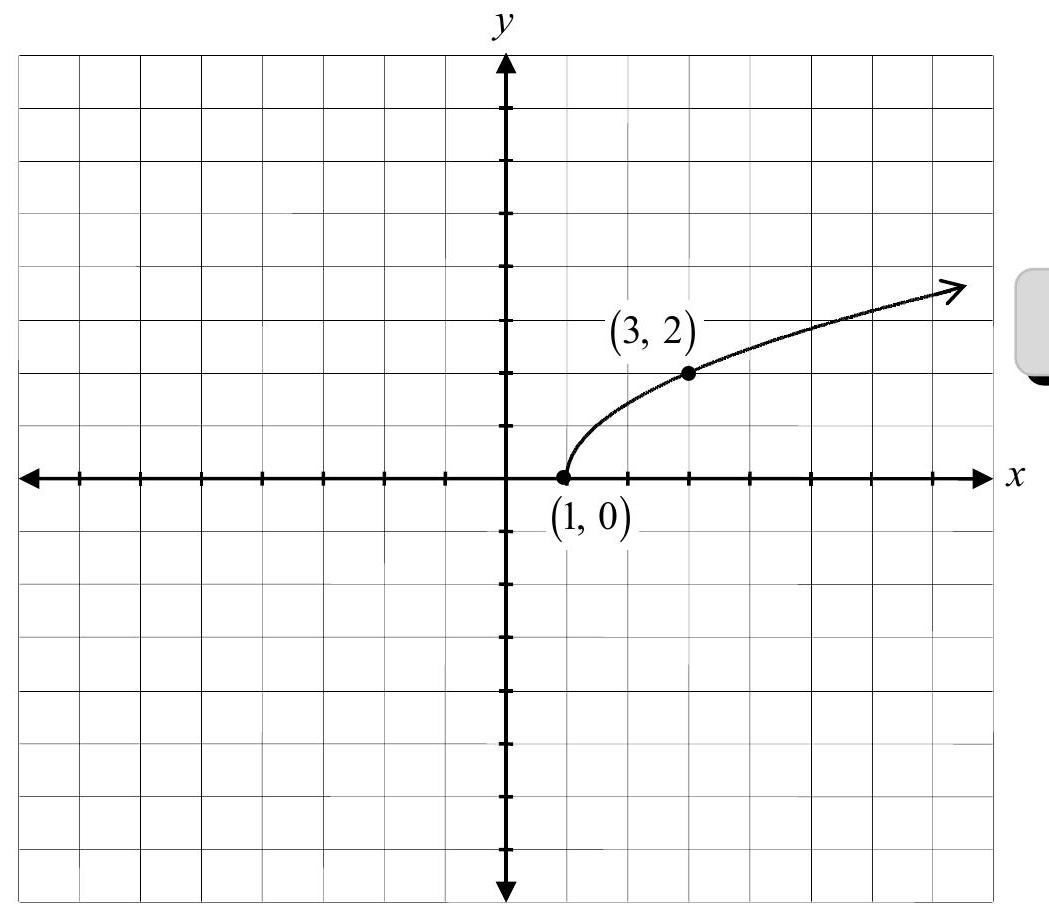
\includegraphics[max width=\textwidth, alt={}]{f67fedaf-ea11-42ad-a16e-f30d2fcf2bd3-030_922_1049_928_163}
\end{center}

1 mark for domain: $[1, \infty)$\\
1 mark for shape (graph of a radical function)\\
1 mark for horizontal compression\\
3 marks

\section*{Method 2}
\begin{center}
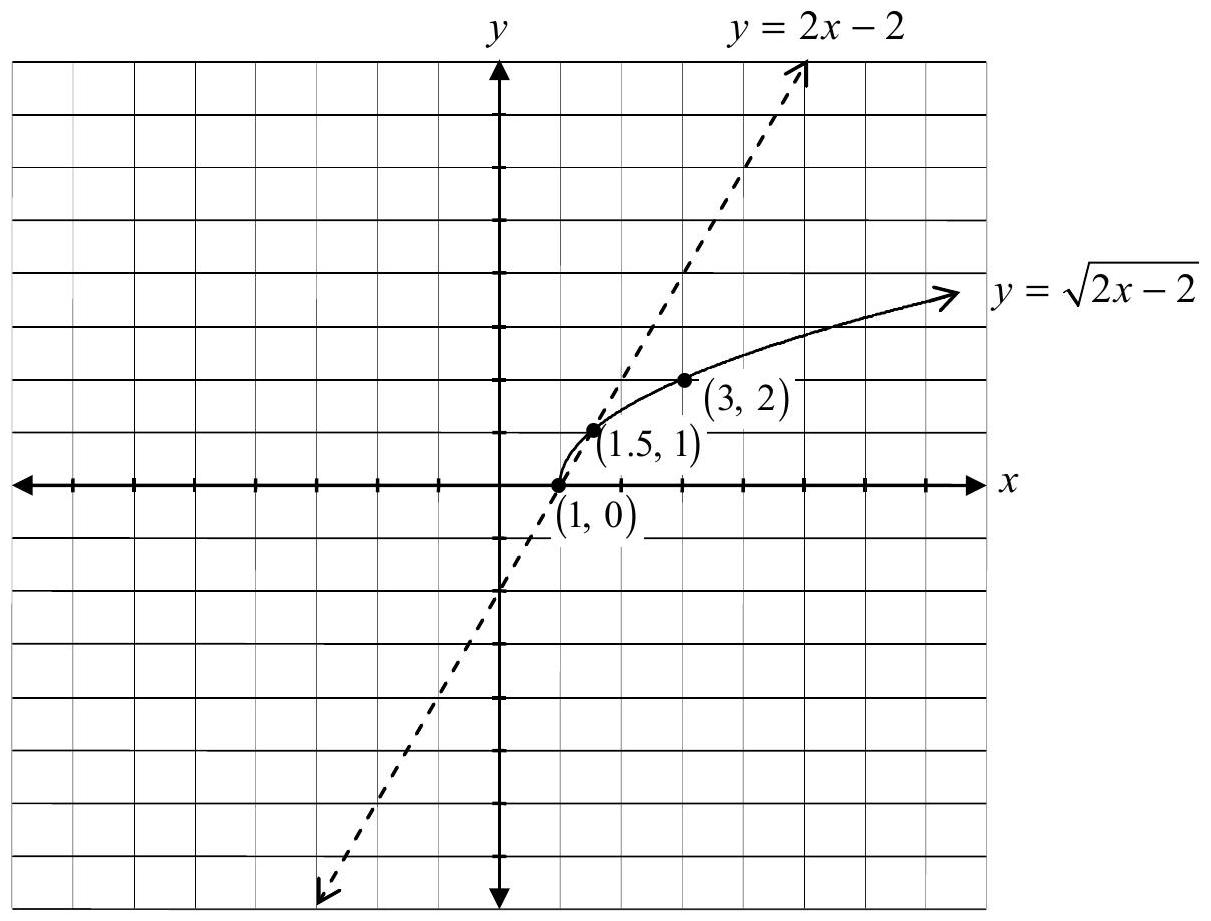
\includegraphics[max width=\textwidth, alt={}]{f67fedaf-ea11-42ad-a16e-f30d2fcf2bd3-031_921_1211_431_223}
\end{center}

1 mark for domain of $y=\sqrt{2 x-2}:[1, \infty)$\\
1 mark for invariant points where $y=0$ and $y=1$ ( $\frac{1}{2}$ mark for each point)\\
$\frac{1}{2}$ mark for graph of $y=\sqrt{2 x-2}$ drawn above the graph of $y=2 x-2$ between the invariant points $\frac{1}{2}$ mark for graph of $y=\sqrt{2 x-2}$ drawn below the graph of $y=2 x-2$ after the invariant point where $y=1$\\
□\\
3 marks

Given $f(x)=2 x-6$, write the equation of $f^{-1}(x)$.

\section*{Solution}
Switch the $x$ and $y$ values.

$$
x=2 y-6
$$

1 mark for switching $x$ and $y$ values

$$
\begin{aligned}
& x+6=2 y \\
& \frac{x+6}{2}=y
\end{aligned}
$$

$\frac{1}{2}$ mark for solving for $y$\\
$\therefore f^{-1}(x)=\frac{x+6}{2}$\\
$\frac{1}{2}$ mark for writing equation of $f^{-1}(x)$

\section*{2 marks}
Question 37\\
R8

Frank tried to expand a logarithmic expression using the laws of logarithms. He made one error.\\
Frank's solution: $\log _{a} \frac{(x+2)}{z w}=\log _{a} x+\log _{a} 2-\log _{a} z-\log _{a} w$\\
Write the correct solution.

\section*{Solution}
Correct solution: $\log _{a} \frac{(x+2)}{z w}=\log _{a}(x+2)-\log _{a} z-\log _{a} w$

1 mark for correct solution\\
1 mark

Determine all non-permissible values of $\theta$ over the interval $[0,2 \pi]$.

$$
\frac{\sin \theta}{1+\cos \theta}+\csc \theta+\cot \theta
$$

Explain your reasoning.

\section*{Solution}
To determine non-permissible values, the denominator 1 mark for explanation needs to equal zero.

The denominators of this expression are " $1+\cos \theta$ " and " $\sin \theta$ " (since $\csc \theta=\frac{1}{\sin \theta}$ and $\cot \theta=\frac{\cos \theta}{\sin \theta}$ ).

1 mark ( $\frac{1}{2}$ mark for identifying each restriction)

$$
\begin{aligned}
\therefore 1+\cos \theta & =0 & \sin \theta & =0 \\
\cos \theta & =-1 & \theta & =0, \pi, 2 \pi \\
\theta & =\pi & &
\end{aligned}
$$

1 mark for all non-permissible values of $\theta$ ( $\frac{1}{2}$ mark for each equation)\\
∴ the non-permissible values of $\theta$ over $[0,2 \pi]$ are $0, \pi$, and $2 \pi$.

Given the following graphs:\\
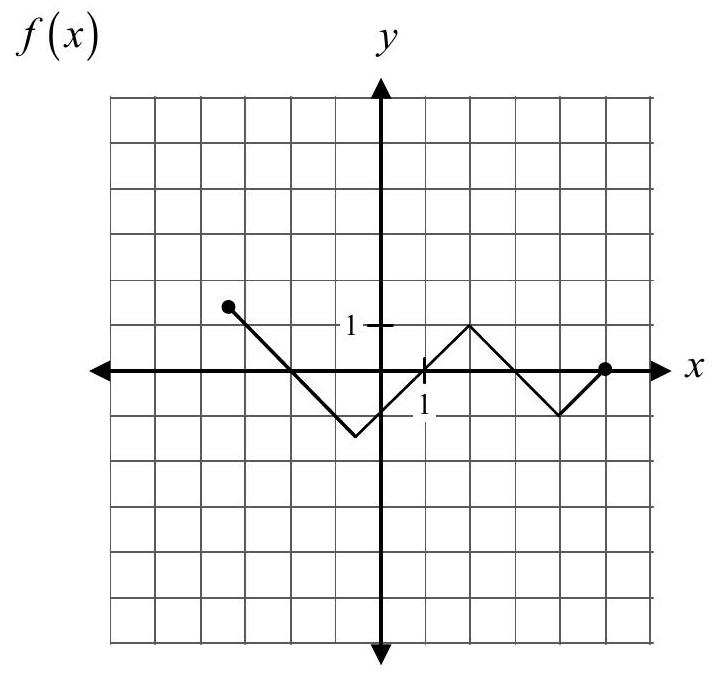
\includegraphics[max width=\textwidth, alt={}, center]{f67fedaf-ea11-42ad-a16e-f30d2fcf2bd3-034_678_717_483_283}\\
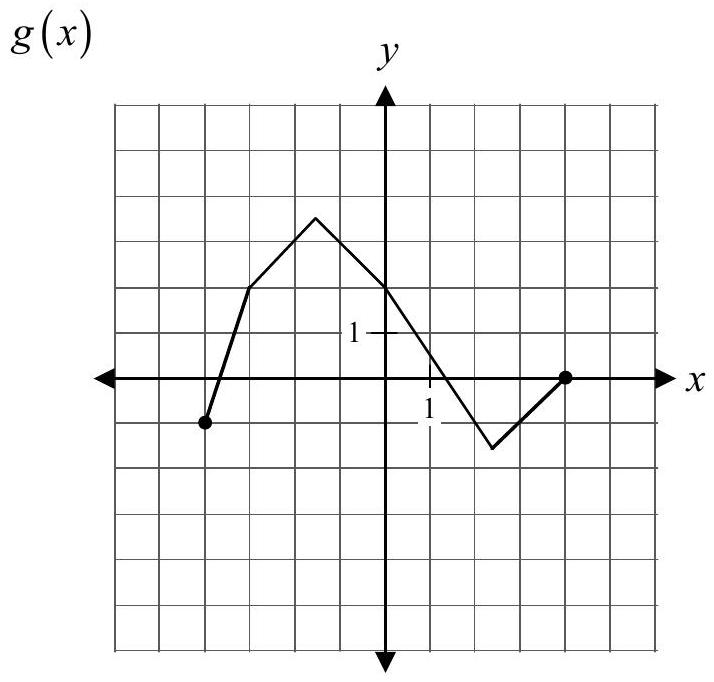
\includegraphics[max width=\textwidth, alt={}, center]{f67fedaf-ea11-42ad-a16e-f30d2fcf2bd3-034_682_714_485_1119}\\
a) Determine the value of $[f \cdot g](0)$.\\
b) Determine the value of $g(f(4))$.\\
c) Determine a value for $k$ where $f(k)=1$.

\section*{Solutions}
a) $f(0)=-1$

$$
g(0)=2
$$

$$
\begin{aligned}
{[f \cdot g](0) } & =(-1)(2) \\
& =-2
\end{aligned}
$$

b) $f(4)=-1$

$$
g(-1)=3
$$

1 mark for the value of $[f \cdot g](0)$

\section*{1 mark}
$\frac{1}{2}$ mark for $f(4)$\\
$\frac{1}{2}$ mark for $g(f(4))$ consistent with $f(4)$ value

\section*{1 mark}
1 mark for a value for $k$\\
1 mark

Given that $h(x)=2 x^{2}+5 x-3$ and that $h(x)=f(x) \cdot g(x)$, determine $f(x)$ and $g(x)$.

\section*{Solution}
$$
\begin{aligned}
& f(x)=2 x-1 \\
& g(x)=x+3
\end{aligned}
$$

1 mark for two correct factors of $h(x)$\\
1 mark\\
Other answers are possible.\\
Question 41

The graph of $y=2 \cos \theta+1$ below can be used to solve the equation $\cos \theta=-\frac{1}{2}$ over the interval $[-2 \pi, 2 \pi]$. Indicate on the graph where to find the solutions to the equation $\cos \theta=-\frac{1}{2}$.

\section*{Solution}
The solution to the equation $\cos \theta=-\frac{1}{2}$ is found where the graph of $y=2 \cos \theta+1$ crosses the $x$-axis.\\
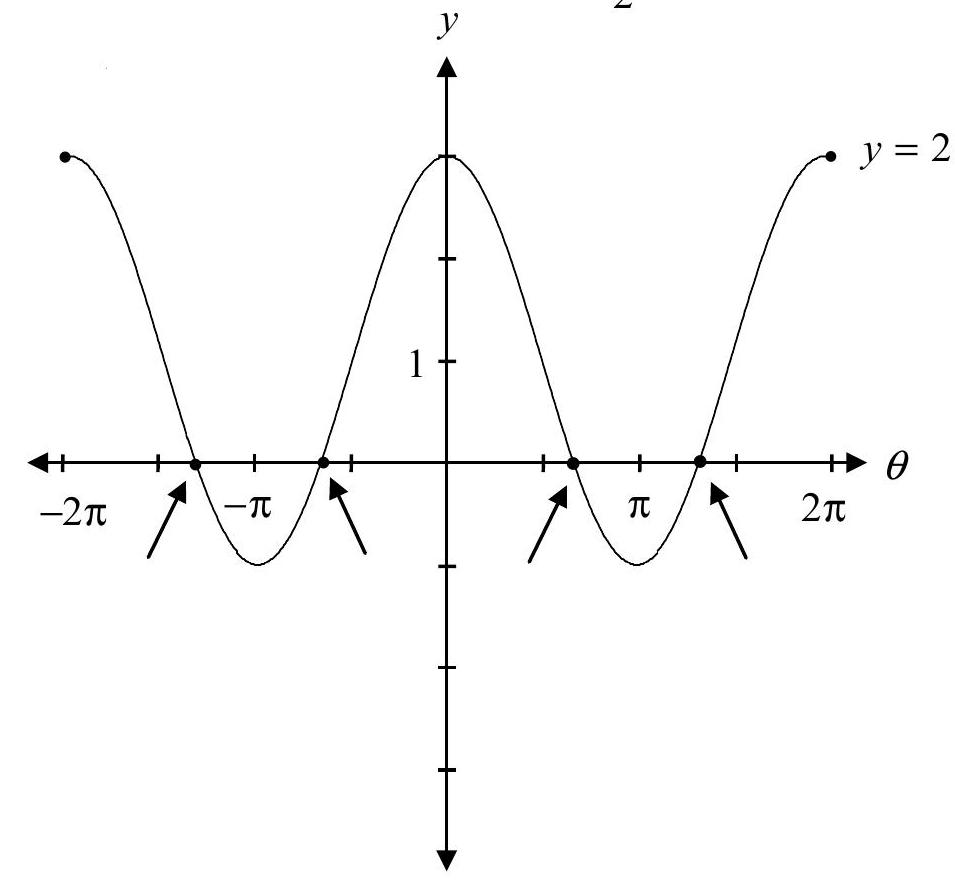
\includegraphics[max width=\textwidth, alt={}, center]{f67fedaf-ea11-42ad-a16e-f30d2fcf2bd3-035_884_955_1499_229}

1 mark for indicating solutions on graph 1 mark

Note(s):

\begin{itemize}
  \item give $\frac{1}{2}$ mark for indicating 1,2 , or 3 of the solutions
\end{itemize}

The function $f(x)$ is transformed.\\
A new function, $y=\frac{1}{f(x)}$, is created that does not have any vertical asymptotes.\\
What can you conclude about the original function $f(x)$ ?

\section*{Solution}
If $f(x)$ does not have any $x$-intercepts, then the transformation would not have any vertical asymptotes.\\
or\\
$f(x)$ cannot equal zero.\\
or

$$
f \neq 0
$$

1 mark for conclusion\\
1 mark

Note(s):

\begin{itemize}
  \item award $\frac{1}{2}$ mark for a correct example without a given conclusion
\end{itemize}

Question 43

Draw the angle $-\frac{7 \pi}{8}$ in standard position.

\section*{Solution}
\begin{center}
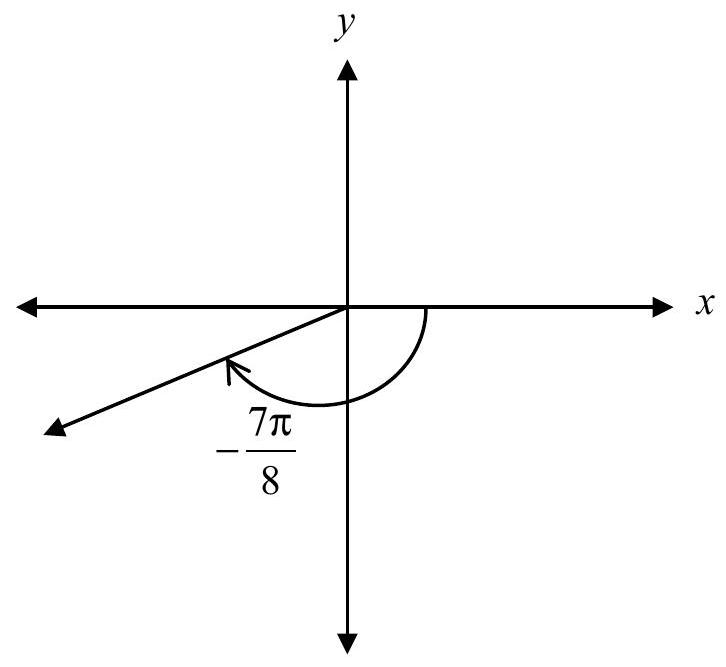
\includegraphics[max width=\textwidth, alt={}]{f67fedaf-ea11-42ad-a16e-f30d2fcf2bd3-036_667_726_1935_216}
\end{center}

1 mark for angle drawn in Quadrant III\\
1 mark

Determine the exact value of:

$$
4 \cos \left(\frac{11 \pi}{12}\right)
$$

\section*{Solution}
\section*{Method 1}
$$
\begin{array}{rlr}
4 \cos \left(\frac{11 \pi}{12}\right) & =4 \cos \left(\frac{\pi}{4}+\frac{2 \pi}{3}\right) & 1 \text { mark for combination } \\
& =4\left[\cos \frac{\pi}{4} \cos \frac{2 \pi}{3}-\sin \frac{\pi}{4} \sin \frac{2 \pi}{3}\right] & \\
& =4\left[\left(\frac{\sqrt{2}}{2}\right)\left(-\frac{1}{2}\right)-\left(\frac{\sqrt{2}}{2}\right)\left(\frac{\sqrt{3}}{2}\right)\right] & 2 \text { marks }\left(\frac{1}{2} \text { mark for each exact value }\right) \\
& =4\left[\frac{-\sqrt{2}-\sqrt{6}}{4}\right] & 3 \text { marks } \\
& =-\sqrt{2}-\sqrt{6}
\end{array}
$$

\section*{Solution}
\section*{Method 2}
$\frac{11 \pi}{12}$ has a reference angle of $\frac{\pi}{12}$.

$$
\begin{aligned}
\cos \left(\frac{\pi}{12}\right) & =\cos \left(\frac{\pi}{4}-\frac{\pi}{6}\right) \\
& =\cos \frac{\pi}{4} \cos \frac{\pi}{6}+\sin \frac{\pi}{4} \sin \frac{\pi}{6} \\
& =\left(\frac{\sqrt{2}}{2}\right)\left(\frac{\sqrt{3}}{2}\right)+\left(\frac{\sqrt{2}}{2}\right)\left(\frac{1}{2}\right) \\
& =\frac{\sqrt{6}+\sqrt{2}}{4}
\end{aligned}
$$

Since $\frac{11 \pi}{12}$ is in Quadrant II, cosine is negative.\\
$\therefore 4 \cos \left(\frac{11 \pi}{12}\right)=4\left(\frac{-\sqrt{6}-\sqrt{2}}{4}\right)$

$$
=-\sqrt{6}-\sqrt{2}
$$

$\frac{1}{2}$ mark for correct reference angle\\
$\frac{1}{2}$ mark for substitution into correct identity

1 mark for exact values

1 mark for the concept that $\cos \left(\frac{11 \pi}{12}\right)$ is $<0$

\section*{3 marks}
Note(s):

\begin{itemize}
  \item $\frac{-2-2 \sqrt{3}}{\sqrt{2}}$ is an acceptable way to write the solution
  \item in Method 1 , another possible combination is $\left(\frac{\pi}{6}+\frac{3 \pi}{4}\right)$
  \item deduct $\frac{1}{2}$ mark if answer is not expressed as a single fraction
  \item in Method 2, the reference angle need not be explicitly stated in order to obtain full marks
\end{itemize}

Sketch the graph of $f(x)=\frac{x-4}{x^{2}-3 x-4}$.

\section*{Solution}
\begin{center}
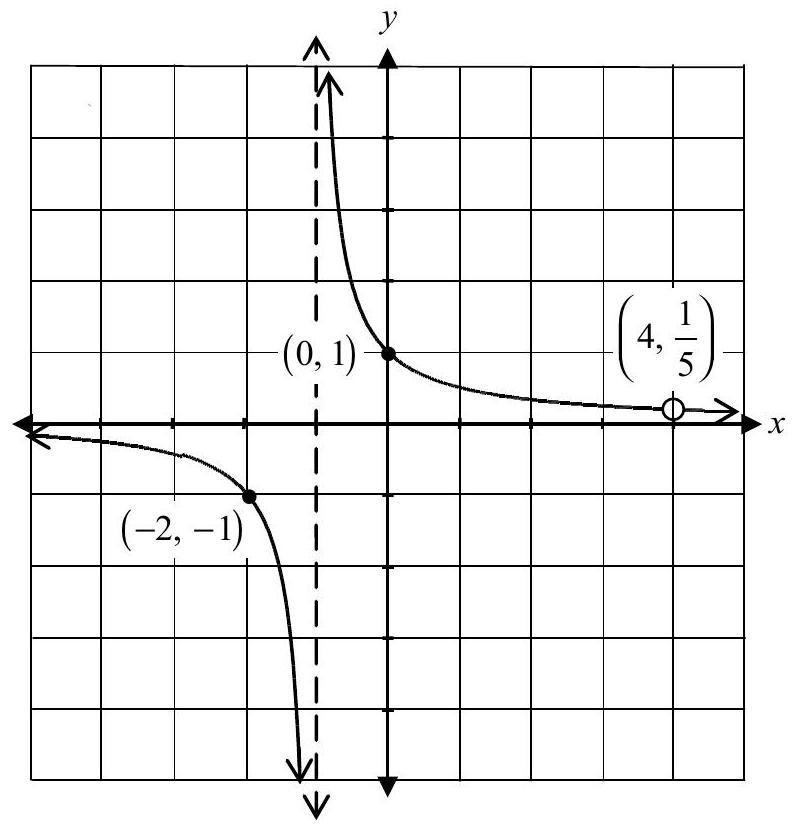
\includegraphics[max width=\textwidth, alt={}]{f67fedaf-ea11-42ad-a16e-f30d2fcf2bd3-039_829_796_708_212}
\end{center}

1 mark for vertical asymptote at $x=-1$\\
$\frac{1}{2}$ mark for graph left of vertical asymptote\\
$\frac{1}{2}$ mark for graph right of vertical asymptote 1 mark for point of discontinuity at $x=4$

3 marks

$$
\begin{aligned}
f(x) & =\frac{x-4}{x^{2}-3 x-4} \\
& =\frac{x-4}{(x-4)(x+1)} \\
& =\frac{1}{x+1} \text { with a point of discontinuity at } x=4
\end{aligned}
$$

point of discontinuity: $f(4)=\frac{1}{5}$\\
∴ there is a point of discontinuity at $\left(4, \frac{1}{5}\right)$

$$
y \text {-intercept: } \begin{aligned}
f(0) & =\frac{0-4}{(0)^{2}-3(0)-4} \\
& =\frac{-4}{-4} \\
& =1
\end{aligned}
$$

Estimate the value of $\log _{5} 35$.\\
Justify your answer.

\section*{Solution}
$$
5^{2}=25 \quad 5^{3}=125
$$

The value of $\log _{5} 35$ is more than 2 but less than 2.5.

$$
\frac{1}{2} \text { mark for justification }
$$

$\frac{1}{2}$ mark for estimated answer

\section*{1 mark}
\section*{Question 47}
If $p(x)=x^{5}-12 x+1$, determine the remainder when $p(x)$ is divided by $(x+2)$.

\section*{Solution}
\section*{Method 1}
$$
\begin{aligned}
p(x) & =x^{5}-12 x+1 \\
p(-2) & =(-2)^{5}-12(-2)+1 \\
& =-32+24+1 \\
& =-7
\end{aligned}
$$

\section*{Method 2}
1 mark for substitution

1 mark

$$
- 2 \longdiv { 1 0 0 0 0 0 0 }
$$

1 mark for correct set-up of synthetic division\\
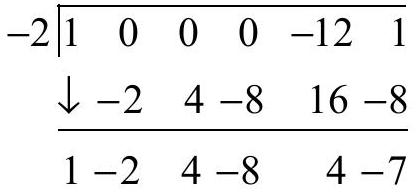
\includegraphics[max width=\textwidth, alt={}, center]{f67fedaf-ea11-42ad-a16e-f30d2fcf2bd3-040_195_418_1963_1138}

1 mark

The remainder is -7 .

Describe the effects on the graph of $y=f(x)$ when asked for the graph of $y=f(x-3)+5$.

\section*{Solution}
Shift right 3 and up $5 \frac{1}{2}$ mark for horizontal translation\\
$\frac{1}{2}$ mark for vertical translation\\
or\\
1 mark\\
$(x+3, y+5)$

Find the exact value of the following expression:

$$
\sin \left(\frac{11 \pi}{3}\right) \cdot \sec \left(\frac{4 \pi}{3}\right) \cdot \tan \left(-\frac{5 \pi}{6}\right)
$$

\section*{Solution}
$=\left(-\frac{\sqrt{3}}{2}\right)(-2)\left(\frac{1}{\sqrt{3}}\right)$\\
1 mark for $\sin \left(\frac{11 \pi}{3}\right)\left(\frac{1}{2}\right.$ mark for quadrant, $\frac{1}{2}$ mark for value $)$\\
$=1$\\
1 mark for $\sec \left(\frac{4 \pi}{3}\right)\left(\frac{1}{2}\right.$ mark for quadrant, $1 / 2$ mark for value)\\
1 mark for $\tan \left(-\frac{5 \pi}{6}\right)\left(\frac{1}{2}\right.$ mark for quadrant, $1 / 2$ mark for value $)$\\
3 marks

Find the coterminal angle to $\frac{27 \pi}{5}$ over the interval $\left[-360^{\circ}, 0^{\circ}\right)$.

\section*{Solution}
\section*{Method 1}
$$
\begin{aligned}
\frac{27 \pi}{5}\left(\frac{180^{\circ}}{\pi}\right) & =27\left(36^{\circ}\right) \\
& =972^{\circ}
\end{aligned}
$$

1 mark for conversion to degrees\\
$\frac{1}{2}$ mark for coterminal angle\\
$\frac{1}{2}$ mark for correct domain

\section*{2 marks}
\section*{Method 2}
$-\frac{3 \pi}{5}$ is a coterminal angle to $\frac{27 \pi}{5}$.\\
$-\frac{3 \pi}{5} \cdot \frac{180^{\circ}}{\pi}=-108^{\circ}$\\
$\frac{1}{2}$ mark for coterminal angle\\
$\frac{1}{2}$ mark for correct domain

1 mark for conversion to degrees\\
2 marks

Solve the following equation over the interval $0 \leq \theta<2 \pi$.

$$
(\tan \theta-3)(\tan \theta+1)=0
$$

\section*{Solution}
$$
\begin{array}{rlr}
\begin{array}{rlr}
(\tan \theta-3)(\tan \theta+1) & =0 & \\
\tan \theta & =3 & \tan \theta \\
\tan & =-1 & 1 \text { mark }(1 / 2 \text { mark for each branch }) \\
\theta_{r} & =1.249046 \quad \theta_{r}= & \frac{\pi}{4} \\
\theta=1.249046 \quad \theta & =\frac{3 \pi}{4}, \frac{7 \pi}{4} & 2 \text { marks }(1 / 2 \text { mark for each value of } \theta) \\
\theta=4.390639 & \quad \text { or } & \mathbf{3} \text { marks } \\
\theta=1.249,4.391 \quad \theta & =2.356194 & \\
\theta & =5.497787 & \\
\theta=1.249, \frac{3 \pi}{4}, 4.391, \frac{7 \pi}{4} & \\
\quad \text { or } & \\
\theta=1.249,2.356,4.391,5.498 &
\end{array}
\end{array}
$$

An earthquake in Vancouver had a magnitude of 6.3 on the Richter scale. An earthquake in Japan had a magnitude of 8.9 on the Richter scale.

How many times more intense was the Japan earthquake than the Vancouver earthquake?\\
You may use the formula below:

$$
M=\log \left(\frac{A}{A_{0}}\right)
$$

where $M$ is the magnitude of the earthquake on the Richter scale\\
$A$ is the intensity of the earthquake\\
$A_{0}$ is the intensity of a standard earthquake\\
Express your answer as a whole number.

\section*{Solution}
\section*{Method 1}
Vancouver: substitute $M=6.3$

$$
\begin{aligned}
6.3 & =\log \left(\frac{A}{A_{0}}\right) \\
10^{6.3} & =\frac{A}{A_{0}} \\
A & =10^{6.3} A_{0}
\end{aligned}
$$

Japan: substitute $M=8.9$

$$
\begin{aligned}
8.9 & =\log \left(\frac{A}{A_{0}}\right) \\
10^{8.9} & =\frac{A}{A_{0}} \\
A & =10^{8.9} A_{0}
\end{aligned}
$$

To compare the two earthquakes divide their intensities.

$$
\begin{aligned}
\frac{\text { the intensity of Japan }}{\text { the intensity of Vancouver }} & =\frac{10^{8.9} A_{0}}{10^{6.3} A_{0}} \\
& =398.107 \\
& =398
\end{aligned}
$$

1 mark for comparison\\
2 marks

\section*{Method 2}
$$
\begin{aligned}
\frac{I_{J}}{I_{V}} & =\frac{10^{8.9}}{10^{6.3}} \\
& =398
\end{aligned}
$$

$$
\begin{aligned}
& 1 \text { mark for comparison } \\
& \frac{1}{2} \text { mark for exponential form } \\
& \frac{1}{2} \text { mark for exponential form } \\
& \mathbf{2} \text { marks }
\end{aligned}
$$

Find and simplify the last term in the expansion of $(2 y-3 x)^{7}$.

\section*{Solution}
$$
\begin{array}{rlr}
t_{8} & ={ }_{7} C_{7}(2 y)^{0}(-3 x)^{7} & \\
& 1 / 2 \text { mark for }{ }_{7} C_{7} \\
& =-2187 x^{7} & \\
& 1 / 2 \text { mark for }(2 y)^{0} \\
& 1 \text { mark for }(-3 x)^{7} \text { which is equal to }-2187 x^{7}
\end{array}
$$

2 marks

Note(s):

\begin{itemize}
  \item no deduction if ${ }_{7} C_{7}$ and $(2 y)^{0}$ are not shown
\end{itemize}

Given $\log _{a} 9=1.129$ and $\log _{a} 4=0.712$, find the value of $\log _{a} 12$.

\section*{Solution}
\section*{Method 1}
$$
\begin{aligned}
\log _{a} 9 & =1.129 \\
\log _{a} 3^{2} & =1.129 \\
2 \log _{a} 3 & =1.129 \\
\log _{a} 3 & =0.5645 \\
\log _{a} 12 & =\log _{a}(4 \cdot 3) \\
& =\log _{a} 4+\log _{a} 3 \\
& =0.712+0.5645 \\
& =1.2765 \\
& =1.277
\end{aligned}
$$

1 mark for power rule

1 mark for writing 12 as a product\\
1 mark for product rule\\
3 marks

\section*{Method 2}
$$
\begin{aligned}
\log _{a} 12 & =\log _{a}(\sqrt{9} \cdot 4) \\
& =\frac{1}{2} \log _{a} 9+\log _{a} 4 \\
& =\frac{1}{2}(1.129)+0.712 \\
& =1.2765 \\
& =1.277
\end{aligned}
$$

1 mark for writing 12 as a product\\
1 mark for power rule\\
1 mark for product rule\\
3 marks

\section*{Method 3}
$$
\begin{aligned}
\log _{a} 9 & =1.129 \\
a^{1.129} & =9 \\
a & =9^{\frac{1}{1.129}} \\
a & =7
\end{aligned}
$$

1 mark for exponential form

1 mark for solving for $a$

$$
\begin{aligned}
\log _{7} 12 & =\frac{\log 12}{\log 7} \\
& =1.276989 \\
& =1.277
\end{aligned}
$$

1 mark for value of $\log _{a} 12$

3 marks

How many different ways can 4 girls and 4 boys be arranged in a row if the girls and the boys must alternate?

\section*{Solution}
\section*{Method 1}
\begin{center}
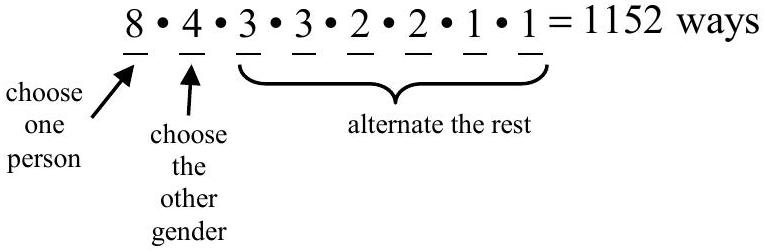
\includegraphics[max width=\textwidth, alt={}]{f67fedaf-ea11-42ad-a16e-f30d2fcf2bd3-049_252_765_655_189}
\end{center}

1 mark for beginning with either gender\\
1 mark for alternating genders

\section*{2 marks}
\section*{Method 2}
Case 1: $\frac{4}{\mathrm{~B}} \cdot \frac{4}{\mathrm{G}} \cdot \frac{3}{\mathrm{~B}} \cdot \frac{3}{\mathrm{G}} \cdot \frac{2}{\mathrm{~B}} \cdot \frac{2}{\mathrm{G}} \cdot \frac{1}{\mathrm{~B}} \cdot \frac{1}{\mathrm{G}}=576$\\
1 mark for arrangement of alternating genders

Case 2: $4 \cdot 4 \cdot 3 \cdot 3 \cdot 2 \cdot 2 \cdot 1 \cdot 1=576$\\
$\frac{1}{2}$ mark for two cases

Total number of ways: $576+576=1152$ ways\\
$\frac{1}{2}$ mark for addition of cases

2 marks

Solve the following equation over the interval $[0,2 \pi]$.

$$
2 \cos 2 \theta-1=0
$$

\section*{Solution}
\section*{Method 1}
$$
\begin{array}{rlrl}
2 \cos 2 \theta-1 & =0 & & \\
2\left(2 \cos ^{2} \theta-1\right)-1 & =0 & & 1 \text { mark for identity } \\
4 \cos ^{2} \theta-3 & =0 & & \\
\cos ^{2} \theta & =\frac{3}{4} & & \\
\cos \theta & = \pm \frac{\sqrt{3}}{2} & 1 \text { mark for solving for } \cos \theta \\
\theta_{r} & =\frac{\pi}{6} & & \\
\theta & =\frac{\pi}{6}, \frac{5 \pi}{6}, \frac{7 \pi}{6}, \frac{11 \pi}{6} & & \begin{array}{l}
2 \text { marks for solutions }(1 / 2 \text { mark for each } \\
\text { consistent solution })
\end{array}
\end{array}
$$

\section*{4 marks}
\section*{Method 2}
$$
y=2 \cos 2 \theta-1
$$

\begin{center}
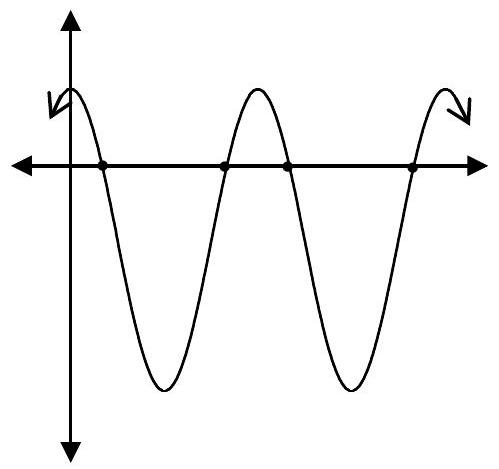
\includegraphics[max width=\textwidth, alt={}]{f67fedaf-ea11-42ad-a16e-f30d2fcf2bd3-050_469_499_1742_176}
\end{center}

1 mark for equation\\
1 mark for the graph with zeroes indicated

2 marks for solutions

\section*{Solution}
\section*{Method 3}
$$
\begin{aligned}
2 \cos 2 \theta-1 & =0 \\
\cos 2 \theta & =\frac{1}{2} \\
\operatorname{let} x & =2 \theta \\
\therefore \cos x & =\frac{1}{2} \\
x_{r} & =\frac{\pi}{3} \\
x & =\frac{\pi}{3}, \frac{5 \pi}{3}, \frac{7 \pi}{3}, \frac{11 \pi}{3} \\
\therefore 2 \theta & =\frac{\pi}{3}, \frac{5 \pi}{3}, \frac{7 \pi}{3}, \frac{11 \pi}{3} \\
\theta & =\frac{\pi}{6}, \frac{5 \pi}{6}, \frac{7 \pi}{6}, \frac{11 \pi}{6}
\end{aligned}
$$

$\frac{1}{2}$ mark for solving for $\cos 2 \theta$\\
$\frac{1}{2}$ mark for reference angle

1 mark for correct angles

1 mark for coterminal angles\\
1 mark for all solutions over the interval $[0,2 \pi]$.\\
4 marks

Note(s):

\begin{itemize}
  \item in Method 1 , deduct a maximum of 1 mark if missing $\cos \theta=-\frac{\sqrt{3}}{2}$
\end{itemize}

Alex incorrectly explains to Rashid that the graph of $y=2 f(x)+5$ means you first move the graph of $y=f(x)$ up 5 units and then multiply the $y$ values by 2 .

Explain to Rashid the correct way to transform the graph.

\section*{Solution}
Alex explains the transformations correctly, but not in the correct order.\\
First multiply the $y$-values by 2 , then move the graph up 5 units.

1 mark for explanation\\
1 mark

Sketch the angle of 5 radians in standard position.

\section*{Solution}
\begin{center}
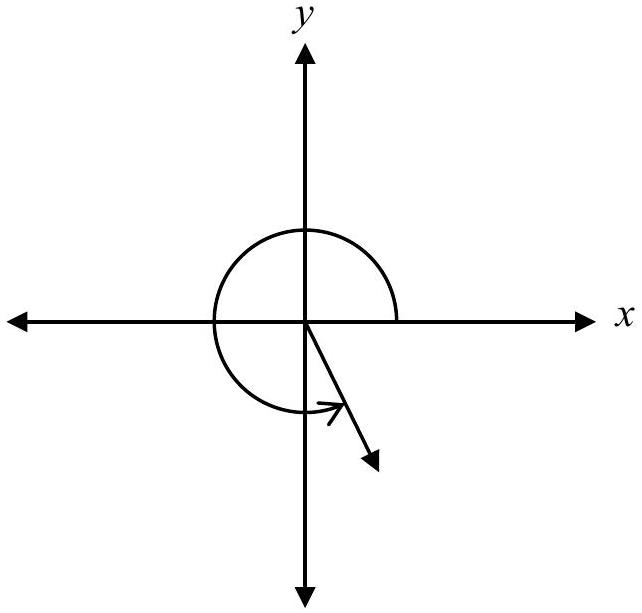
\includegraphics[max width=\textwidth, alt={}]{f67fedaf-ea11-42ad-a16e-f30d2fcf2bd3-053_613_642_623_186}
\end{center}

1 mark for angle drawn in Quadrant IV\\
1 mark

Given the graphs of $f(x)$ and $(f-g)(x)$, sketch the graph of $g(x)$.\\
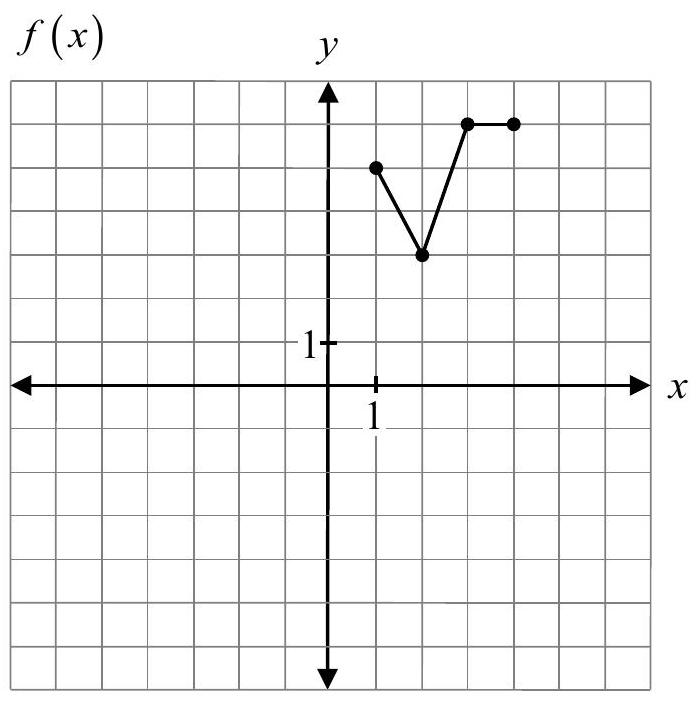
\includegraphics[max width=\textwidth, alt={}, center]{f67fedaf-ea11-42ad-a16e-f30d2fcf2bd3-054_701_699_558_206}\\
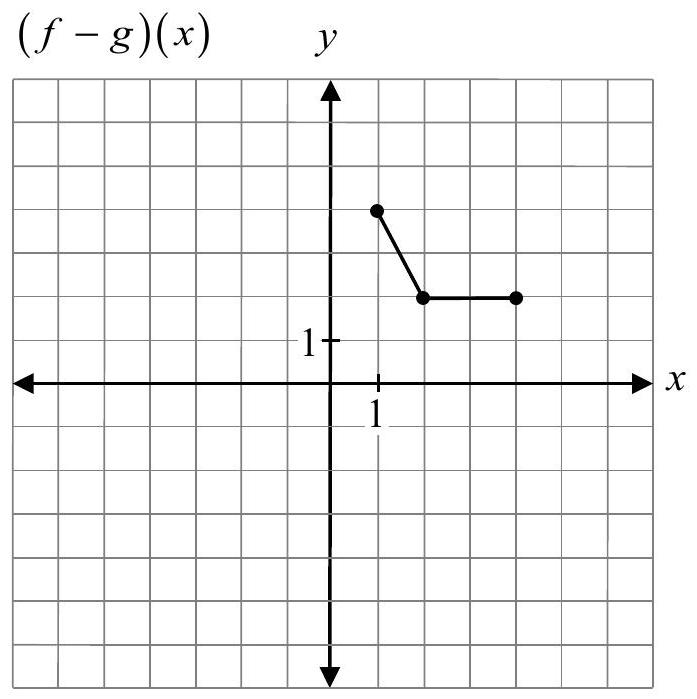
\includegraphics[max width=\textwidth, alt={}, center]{f67fedaf-ea11-42ad-a16e-f30d2fcf2bd3-054_699_697_560_1078}

\section*{Solution}
\begin{center}
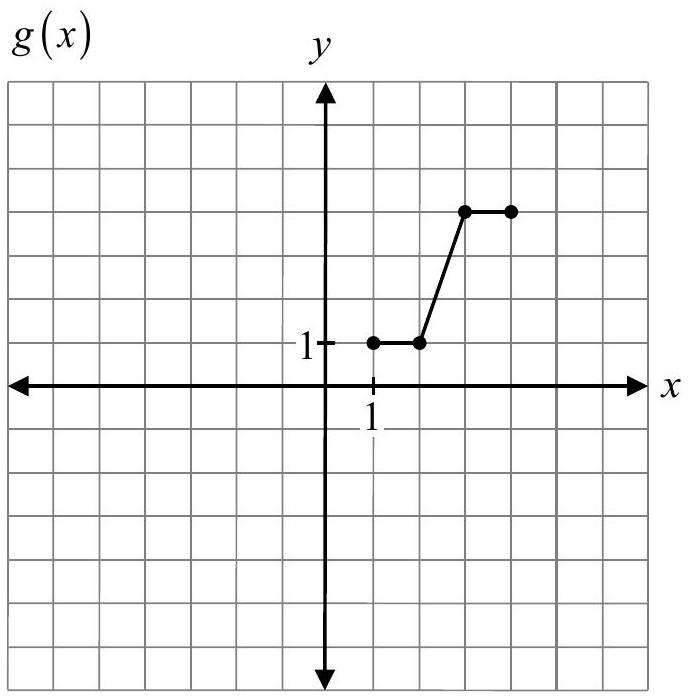
\includegraphics[max width=\textwidth, alt={}]{f67fedaf-ea11-42ad-a16e-f30d2fcf2bd3-054_700_691_1516_197}
\end{center}

1 mark for subtraction of $f(x)-(f-g)(x)$ 1 mark for shape representing the operation given

A particular math class has a large number of students. From this class, you are to create a committee of 4 students that has at least 1 girl.

Without actually solving the problem, explain the strategy you would use to find the total number of ways to select this committee.

\section*{Solution}
\section*{Method 1}
Find all ways to form the committee and subtract the number of ways with no girls on the committee.\\
1 mark for identifying cases\\
1 mark for operation on these cases\\
2 marks

\section*{Method 2}
Find all scenarios with girls on the committee: 1 girl on the committee, 2 girls on the committee, 3 girls on the committee, and a committee with all girls. Then add all scenarios together to get the total number of ways to create a committee with at least 1 girl.

1 mark for identifying cases\\
1 mark for operation on these cases\\
2 marks

Note(s):

\begin{itemize}
  \item in Method 2, deduct $\frac{1}{2}$ mark if one of the cases is missing\\
a) Prove the identity below for all permissible values of $\theta$.
\end{itemize}

$$
\frac{1+2 \cos ^{2} \theta}{\cos ^{2} \theta}=\tan ^{2} \theta+3
$$

b) Determine all the non-permissible values for $\theta$.

\section*{Solution}
\section*{Method 1}
a)

\begin{center}
\begin{tabular}{l|c}
\multicolumn{1}{c|}{LHS} & RHS \\
\hline
$\frac{1}{\cos ^{2} \theta}+\frac{2 \cos ^{2} \theta}{\cos ^{2} \theta}$ & $\tan ^{2} \theta+3$ \\
$\sec ^{2} \theta+2$ &  \\
$\tan ^{2} \theta+1+2$ &  \\
$\tan ^{2} \theta+3$ &  \\
\end{tabular}
\end{center}

$$
\therefore \mathrm{LHS}=\mathrm{RHS}
$$

b) $\quad \cos ^{2} \theta=0$

$$
\begin{aligned}
\cos \theta & =0 \\
\theta & =\frac{\pi}{2}, \frac{3 \pi}{2}, \ldots
\end{aligned}
$$

$\frac{1}{2}$ mark for $\cos ^{2} \theta=0$\\
$\frac{1}{2}$ mark for any non-permissible value of $\theta$\\
∴ the non-permissible values of $\theta$\\
are $\frac{\pi}{2}+k \pi, k \in \mathrm{I}$\\
or\\
1 mark for all non-permissible values of $\theta$

1 mark for appropriate algebraic strategy\\
1 mark for appropriate identity substitutions

\section*{2 marks}
$90^{\circ}+180 k, k \in \mathrm{I}$.

\section*{Solution}
\section*{Method 2}
a)

\begin{center}
\begin{tabular}{l|l}
LHS & \multicolumn{1}{|c}{RHS} \\
\hline
$\frac{1+2 \cos ^{2} \theta}{\cos ^{2} \theta}$ & $\tan ^{2} \theta+3$ \\
 & $\sec ^{2} \theta-1+3$ \\
 & $\sec ^{2} \theta+2$ \\
 & $\frac{1}{\cos ^{2} \theta}+2$ \\
 & $\frac{1}{\cos ^{2} \theta}+\frac{2 \cos ^{2} \theta}{\cos ^{2} \theta}$ \\
 & $\frac{1+2 \cos ^{2} \theta}{\cos ^{2} \theta}$ \\
\end{tabular}
\end{center}

∴ LHS $=$ RHS\\
b) $\quad \cos ^{2} \theta=0$\\
$\cos \theta=0$

$$
\theta=\frac{\pi}{2}, \frac{3 \pi}{2}, \ldots
$$

∴ the non-permissible values of $\theta$\\
are $\frac{\pi}{2}+k \pi, k \in \mathrm{I}$\\
or\\
$90^{\circ}+180 k, k \in \mathrm{I}$.

1 mark for appropriate identity substitutions 1 mark for appropriate algebraic strategy\\
$\frac{1}{2}$ mark for $\cos ^{2} \theta=0$\\
$\frac{1}{2}$ mark for any non-permissible value of $\theta$ 1 mark for all non-permissible values of $\theta$

2 marks

Given the graph of $f(x)$ below, sketch the graph of $g(x)=f(x-2)+3$.\\
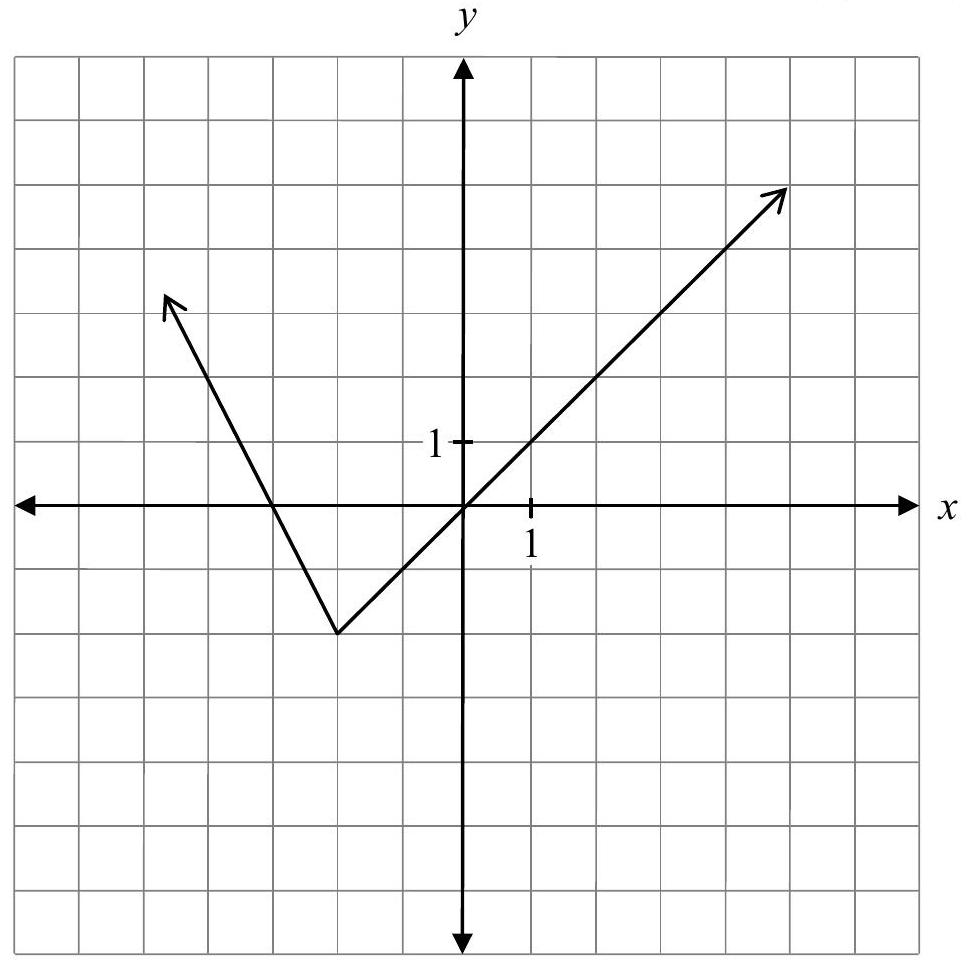
\includegraphics[max width=\textwidth, alt={}, center]{f67fedaf-ea11-42ad-a16e-f30d2fcf2bd3-058_968_972_446_294}

\section*{Solution}
\begin{center}
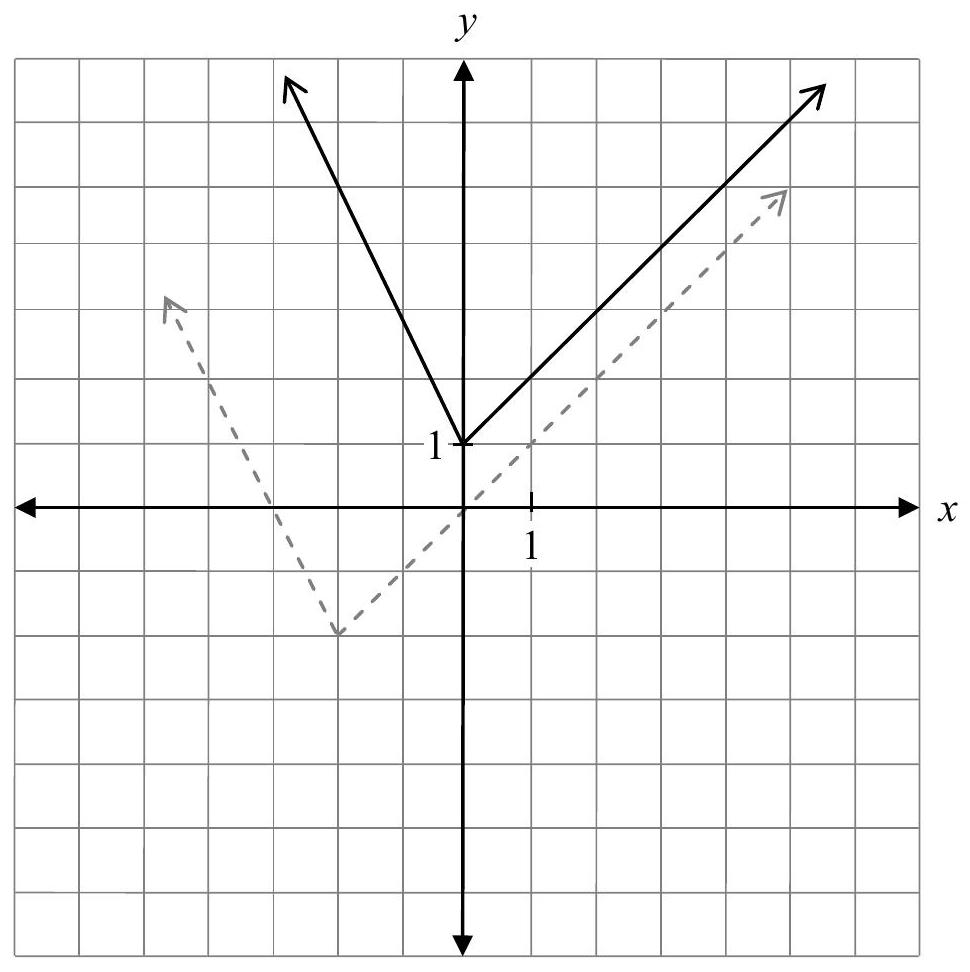
\includegraphics[max width=\textwidth, alt={}]{f67fedaf-ea11-42ad-a16e-f30d2fcf2bd3-058_972_970_1531_300}
\end{center}

1 mark for horizontal shift 1 mark for vertical shift

2 marks

Given that $\sin \alpha=\frac{5}{13}$, where $\alpha$ is in Quadrant II, and $\cos \beta=\frac{2}{5}$, where $\beta$ is in Quadrant IV, find the exact value of:\\
a) $\cos (\alpha+\beta)$\\
b) $\quad \sin 2 \alpha$

\section*{Solution}
a)\\
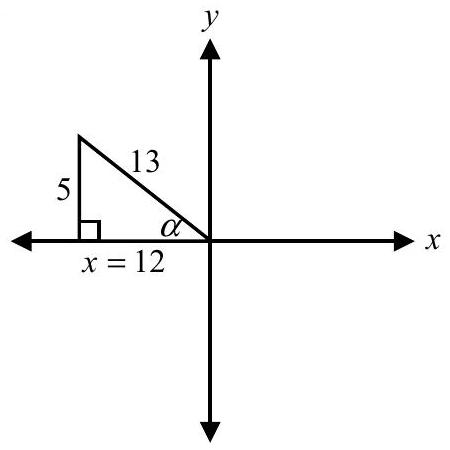
\includegraphics[max width=\textwidth, alt={}, center]{f67fedaf-ea11-42ad-a16e-f30d2fcf2bd3-059_450_450_739_210}

$$
\begin{aligned}
x^{2}+y^{2} & =r^{2} \\
x^{2}+25 & =169 \\
x^{2} & =144 \\
x & = \pm 12 \\
x & =-12
\end{aligned}
$$

$$
\begin{aligned}
x^{2}+y^{2} & =r^{2} \\
4+y^{2} & =25 \\
y^{2} & =21 \\
y & = \pm \sqrt{21} \\
y & =-\sqrt{21}
\end{aligned}
$$

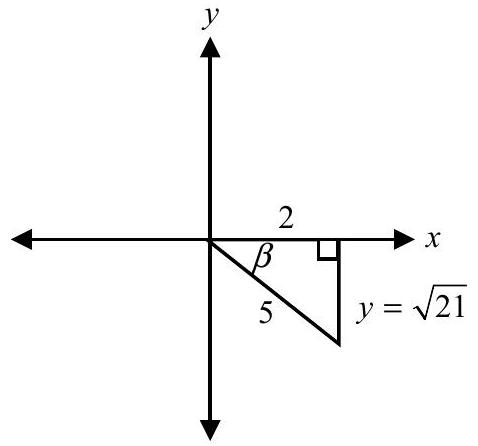
\includegraphics[max width=\textwidth, alt={}, center]{f67fedaf-ea11-42ad-a16e-f30d2fcf2bd3-059_446_478_708_1437}\\
$\frac{1}{2}$ mark for value of $x$\\
$\frac{1}{2}$ mark for value of $y$

$$
\begin{aligned}
\cos (\alpha+\beta) & =\cos \alpha \cos \beta-\sin \alpha \sin \beta \\
& =\left(-\frac{12}{13}\right)\left(\frac{2}{5}\right)-\left(\frac{5}{13}\right)\left(-\frac{\sqrt{21}}{5}\right) \quad \begin{array}{l}
1 / 2 \text { mark for } \cos \alpha \\
1 / 2 \text { mark for } \sin \beta
\end{array}
\end{aligned}
$$

$$
\begin{aligned}
& =-\frac{24}{65}+\frac{5 \sqrt{21}}{65} \\
& =\frac{5 \sqrt{21}-24}{65}
\end{aligned}
$$

1 mark for substitution into correct identity

\section*{3 marks}
b) $\quad \sin 2 \alpha=2 \sin \alpha \cos \alpha$

$$
\begin{aligned}
& =2\left(\frac{5}{13}\right)\left(-\frac{12}{13}\right) \\
& =-\frac{120}{169}
\end{aligned}
$$

1 mark for substitution into correct identity

\section*{1 mark}
Note(s):

\begin{itemize}
  \item accept any of the following values for $x$ : $x= \pm 12, x=-12$ or $x=12$
  \item accept any of the following values for $y: y= \pm \sqrt{21}, y=-\sqrt{21}$ or $y=\sqrt{21}$
\end{itemize}

If $f(x)=x^{3}$ and $g(x)=2 x-3$, what is the value of $\left(\frac{f}{g}\right)(-1)$ ?

\section*{Solution}
$$
\begin{aligned}
f(-1) & =(-1)^{3} \\
& =-1 \\
g(-1) & =2(-1)-3 \\
& =-5
\end{aligned}
$$

$\frac{1}{2}$ mark for substituting into $f(x)$ and $g(x)$

$$
\begin{aligned}
\left(\frac{f}{g}\right)(-1) & =\frac{-1}{-5} \\
& =\frac{1}{5}
\end{aligned}
$$

$$
\begin{aligned}
& \frac{1}{2} \text { mark for evaluating }\left(\frac{f}{g}\right)(-1) \\
& \mathbf{1} \text { mark }
\end{aligned}
$$

If the point $(4,-3)$ lies on the graph of $f(x)$, which point must lie on the graph of $2 f(2 x)$ ?\\
a) $(8,-6)$\\
b) $(2,-6)$\\
c) $\left(8,-\frac{3}{2}\right)$\\
d) $\left(2,-\frac{3}{2}\right)$

Question 17

The graph of $y=\log _{2}(2 x+6)$ intersects the graph of $y=4$ at:\\
a) $x=-1$\\
b) $x=1$\\
c) $x=5$\\
d) $x=14$

Question 18

Given the point $\mathrm{A}(-3,5)$ on the terminal arm of an angle $\theta$, identify the value of $\cot \theta$.\\
a) $-\frac{3}{5}$\\
b) $-\frac{5}{3}$\\
c) $-\frac{4}{5}$\\
d) $-\frac{5}{4}$

The graph of $y=\left(\frac{1}{2}\right)^{x}$ compared to the graph of $x=\left(\frac{1}{2}\right)^{y}$ is a:\\
a) reflection in the $x$-axis\\
b) reflection in the $y$-axis\\
c) reflection in the line $y=x$\\
d) reciprocal function

Question 20\\
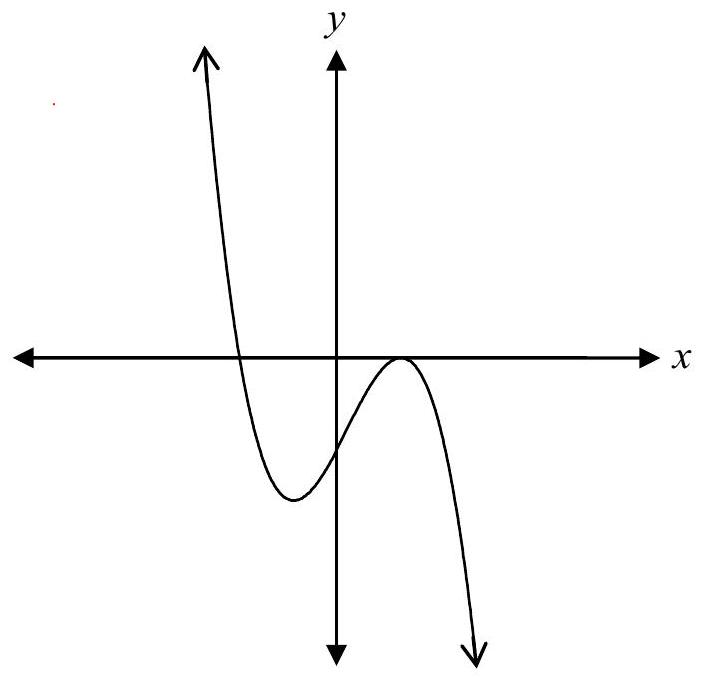
\includegraphics[max width=\textwidth, alt={}, center]{f67fedaf-ea11-42ad-a16e-f30d2fcf2bd3-062_679_706_1188_313}

Given the above graph of a polynomial function, which one of the following statements can be true?\\
a) The function has a degree of 4 with a positive leading coefficient.\\
b) The function has a degree of 4 with a negative leading coefficient.\\
c) The function has a degree of 3 with a positive leading coefficient.\\
d) The function has a degree of 3 with a negative leading coefficient.

Given that $(x+3)$ is a factor of polynomial $P(x)$, which of the following is true?\\
a) $P(-3)=0$\\
b) $P(0)=-3$\\
c) $P(0)=3$\\
d) $P(3)=0$

Question 22

Which of the following is a reasonable estimate for the value of $\log 350$ ?\\
a) 2\\
b) 2.5\\
c) 2.8\\
d) 3

Question 23

The graph of the function $f(x)$ shown below is best described by the equation:\\
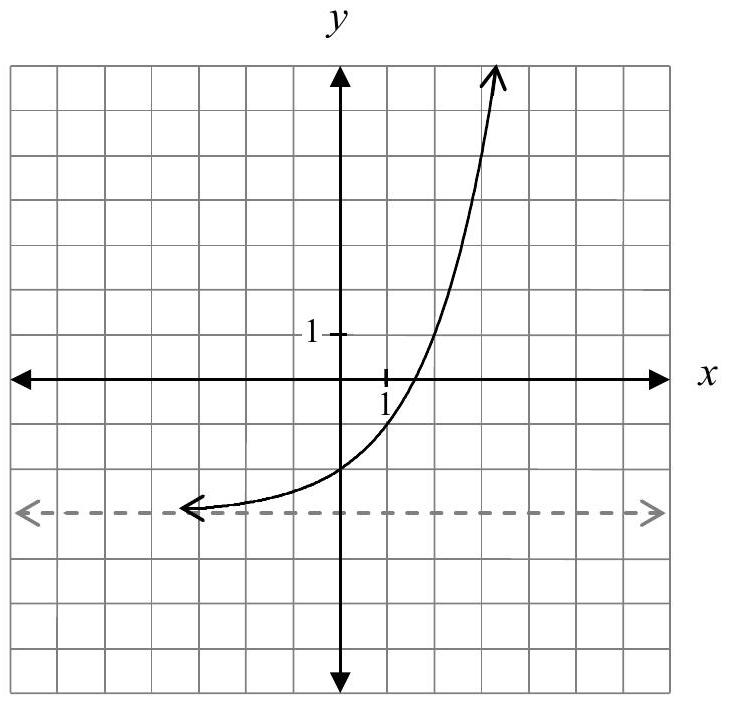
\includegraphics[max width=\textwidth, alt={}, center]{f67fedaf-ea11-42ad-a16e-f30d2fcf2bd3-063_703_729_1624_262}\\
a) $f(x)=2^{x+3}$\\
b) $f(x)=2^{x}+3$\\
c) $f(x)=2^{x-3}$\\
d) $f(x)=2^{x}-3$

Given the graph of $y=f(x)$, what is the domain of $\sqrt{f(x)}$ ?\\
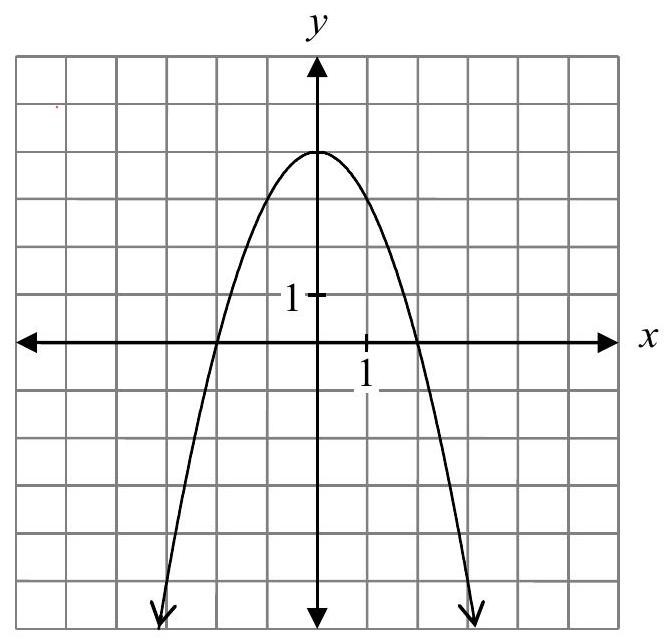
\includegraphics[max width=\textwidth, alt={}, center]{f67fedaf-ea11-42ad-a16e-f30d2fcf2bd3-064_640_671_491_247}\\
a) $x \in \mathbb{R}$\\
b) $-2 \leq x \leq 2$\\
c) $x \leq-2$ or $x \geq 2$\\
d) $0 \leq x \leq 4$

Question 25

Solve:

$$
e^{\ln (5-x)}=7
$$

a) -2\\
b) $-\ln 2$\\
c) $\ln 7-\ln 5$\\
d) $\frac{7}{5}$

One of the factors of $P(x)=x^{3}-k x^{2}-7 x+10$ is $(x-2)$.\\
Find the value of $k$.

\section*{Solution}
\section*{Method 1}
$$
x=2
$$

$$
\begin{aligned}
0 & =(2)^{3}-k(2)^{2}-7(2)+10 \\
0 & =8-4 k-14+10 \\
0 & =4-4 k \\
4 k & =4 \\
k & =1
\end{aligned}
$$

$\frac{1}{2}$ mark for $x=2$

1 mark for remainder theorem\\
$\frac{1}{2}$ mark for solving for $k$

\section*{2 marks}
$\frac{1}{2}$ mark for $x=2$\\
$\frac{1}{2}$ mark for synthetic division\\
$\frac{1}{2}$ mark for equating the remainder to zero\\
$\frac{1}{2}$ mark for solving for $k$\\
2 marks\\
a) Sketch the graph of the function $y=\sqrt{-x}+1$.

\section*{Solution}
\begin{center}
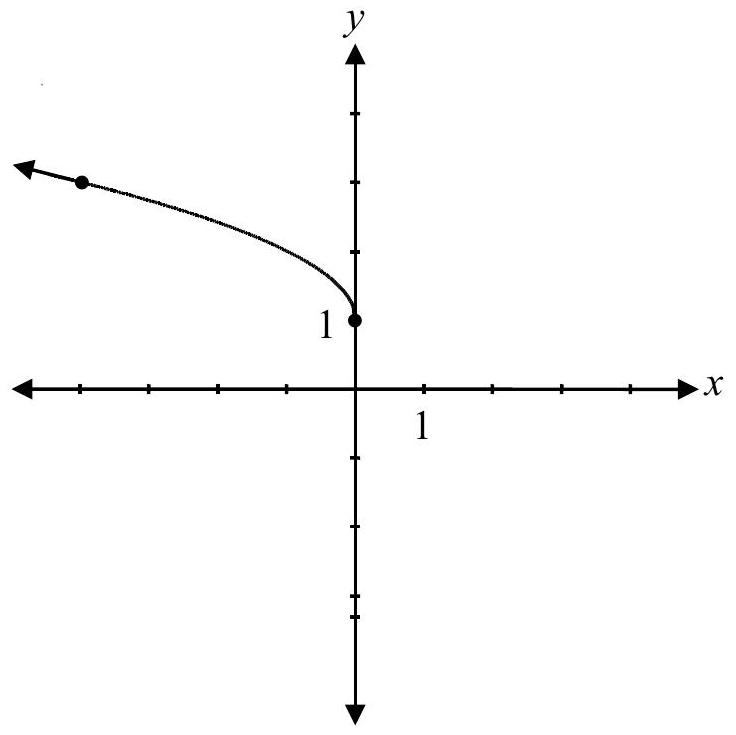
\includegraphics[max width=\textwidth, alt={}]{f67fedaf-ea11-42ad-a16e-f30d2fcf2bd3-066_735_736_522_251}
\end{center}

1 mark for general shape 1 mark for horizontal reflection 1 mark for vertical shift\\
b) Determine the value of $x$ when $y=3$.

\section*{Method 1}
\begin{center}
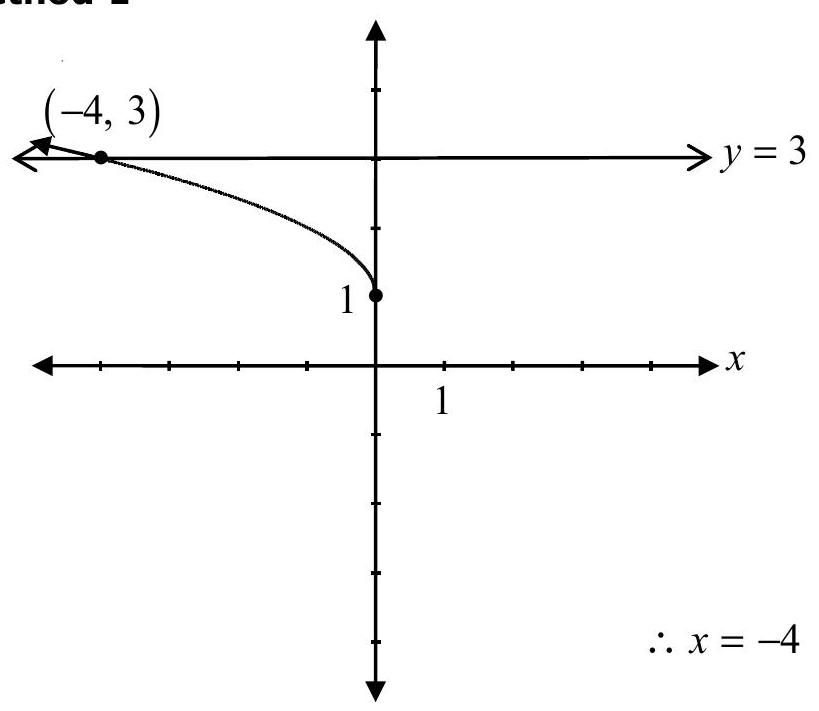
\includegraphics[max width=\textwidth, alt={}]{f67fedaf-ea11-42ad-a16e-f30d2fcf2bd3-066_711_819_1386_227}
\end{center}

\section*{Method 2}
1 mark for consistent value of $x$\\
1 mark

$$
\begin{aligned}
& y=\sqrt{-x}+1 \\
& 3=\sqrt{-x}+1 \\
& 2=\sqrt{-x} \\
& 4=-x \\
& x=-4
\end{aligned}
$$

1 mark for consistent value of $x$

Solve the following equation:

$$
{ }_{n} P_{2}={ }_{n} C_{3}
$$

\section*{Solution}
\section*{Method 1}
$$
\begin{aligned}
\frac{n!}{(n-2)!} & =\frac{n!}{(n-3)!3!} \\
n!(n-3)!3! & =n!(n-2)! \\
6 & =\frac{(n-2)!}{(n-3)!} \\
6 & =\frac{(n-2)(n-3)!}{(n-3)!} \\
6 & =n-2 \\
8 & =n
\end{aligned}
$$

\section*{Method 2}
$$
\begin{aligned}
{ }_{n} P_{2} & ={ }_{n} C_{3} ; \text { we know } n \geq 3 \\
\frac{n!}{(n-2)!} & =\frac{n!}{(n-3)!3!} \\
\frac{n(n-1)(n-2)!}{(n-2)!} & =\frac{n(n-1)(n-2)(n-3)!}{(n-3)!6 \quad \text { we can divide by } n} \\
6 & =\frac{n(n-1)(n-2)}{n(n-1)} \quad \text { and }(n-1) \text { since } \\
6 & =n-2 \\
8 & =n
\end{aligned}
$$

$\frac{1}{2}$ mark for substituting for ${ }_{n} P_{2}$\\
$\frac{1}{2}$ mark for substituting for ${ }_{n} C_{3}$\\
1 mark for simplification

1 mark for expansion of $(n-2)$ !

\section*{3 marks}
$\frac{1}{2}$ mark for substituting for ${ }_{n} P_{2}$\\
$\frac{1}{2}$ mark for substituting for ${ }_{n} C_{3}$\\
$\frac{1}{2}$ mark for expansion of ${ }_{n} P_{2}$\\
$\frac{1}{2}$ mark for expansion of ${ }_{n} C_{3}$

1 mark for simplification\\
3 marks

\section*{Solution}
\section*{Method 3}
$$
\begin{array}{rlrl}
{ }_{n} P_{2} & ={ }_{n} C_{3} & & \\
\frac{n!}{(n-2)!} & =\frac{n!}{(n-3)!3!} & & 1 / 2 \text { mark for substituting for }{ }_{n} P_{2} \\
\frac{n(n-1)(n-2)!}{(n-2)!} & =\frac{n(n-1)(n-2)(n-3)!}{(n-3)!3!} & & 1 / 2 \text { mark for substituting for }{ }_{n} C_{3} \\
6 n(n-1) & =n(n-1)(n-2) & & 1 / 2 \text { mark for expansion of }{ }_{n} P_{2} \\
{ }_{n} C_{3} & &
\end{array}
$$

$6 n(n-1)-n(n-1)(n-2)=0$

$$
n(n-1)(6-(n-2))=0
$$

$$
n(n-1)(8-n)=0
$$

1 mark for simplification

Note(s):

\begin{itemize}
  \item deduct $\frac{1}{2}$ mark for not rejecting non-permissible values
\end{itemize}

Given $f(x)=x^{2}-1$ and $g(x)=\sqrt{x+1}$, sketch the graph of $y=f(g(x))$ and state its domain.

\section*{Solution}
\section*{Method 1}
$f(x)=x^{2}-1$\\
Domain: $x \in \mathbb{R}$

$$
\begin{aligned}
f(g(x)) & =(\sqrt{x+1})^{2}-1 \\
& =x+1-1 \\
& =x
\end{aligned}
$$

\begin{center}
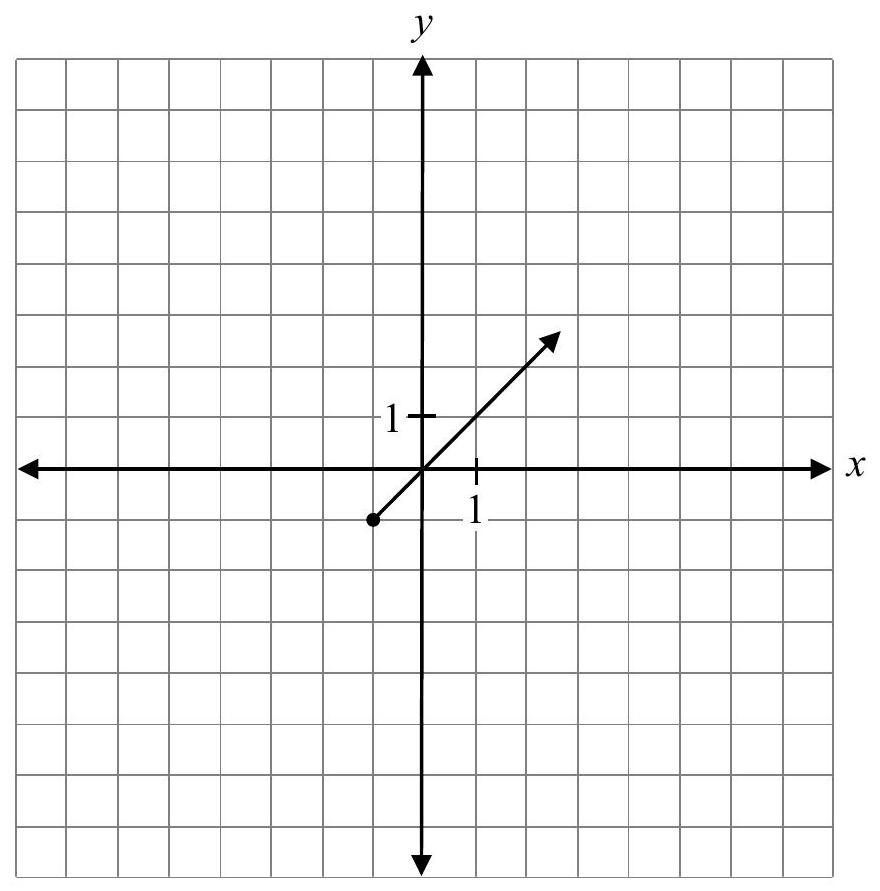
\includegraphics[max width=\textwidth, alt={}]{f67fedaf-ea11-42ad-a16e-f30d2fcf2bd3-069_891_880_1123_182}
\end{center}

Domain of $f(g(x)):[-1, \infty) \quad$ or $\quad\{x \mid x \geq-1, x \in \mathbb{R}\} \quad 1$ mark for restricted domain

\section*{Solution}
\section*{Method 2}
\begin{center}
\begin{tabular}{r|c|c}
$x$ & $g(x)$ & $f(g(x))$ \\
\hline
-2 &  &  \\
-1 & 0 & -1 \\
0 & 1 & 0 \\
1 &  & 1 \\
2 &  & 2 \\
3 & 2 & 3 \\
\end{tabular}
\end{center}

1 mark for table of values\\
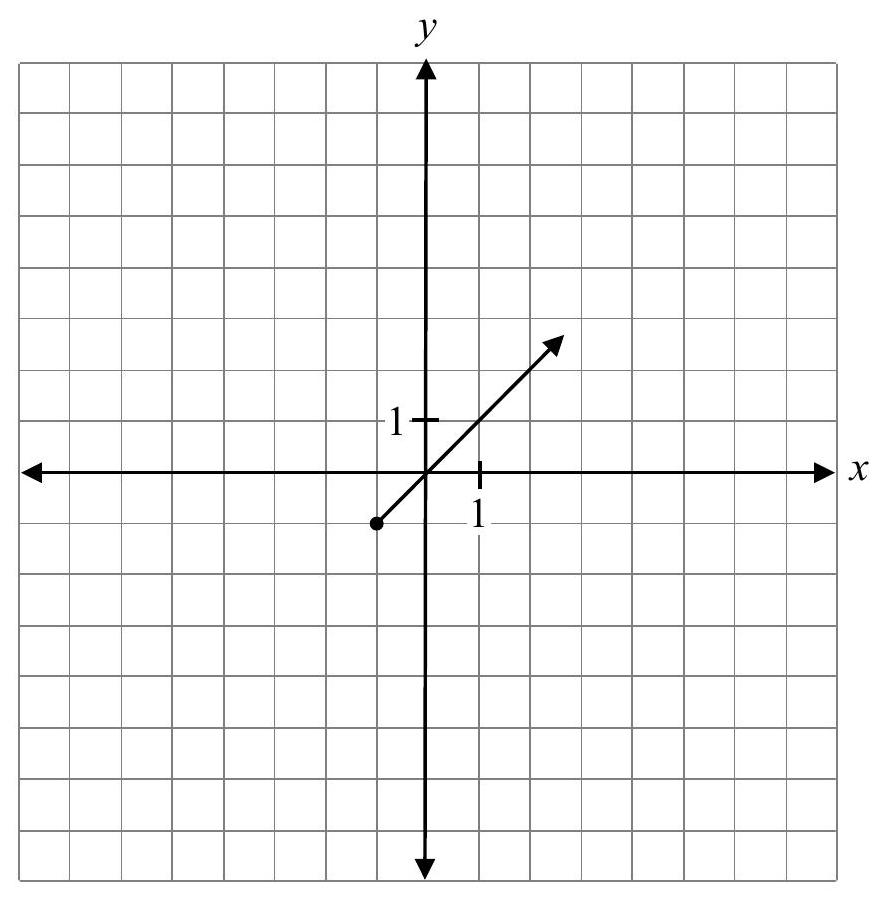
\includegraphics[max width=\textwidth, alt={}, center]{f67fedaf-ea11-42ad-a16e-f30d2fcf2bd3-070_897_884_983_178}

1 mark for graph of composite function

Domain of $f(g(x)):[-1, \infty) \quad$ or $\quad\{x \mid x \geq-1, x \in \mathbb{R}\}$\\
1 mark for restricted domain\\
3 marks

Write the equation of the horizontal asymptote for the function $f(x)=\frac{x-3}{x-2}$.

\section*{Solution}
$y=1$\\
1 mark for equation of horizontal asymptote\\
1 mark

The $x$-intercept of $f(x)$ is 4 and the $x$-intercept of $g(x)$ is 4 .\\
Benjamin concludes that the $x$-intercept of $f(x)+g(x)$ is 8 .\\
Do you agree with Benjamin? Justify your answer.

\section*{Solution}
No, I do not agree with Benjamin.\\
Benjamin added the $x$-values instead of adding the $y$-values.\\
If the $x$-intercept of $f(x)$ is 4 , then $y=0$.\\
If the $x$-intercept of $g(x)$ is 4 , then $y=0$.\\
∴ the $x$-intercept of $f(x)+g(x)$ is 4 .

1 mark for justification\\
1 mark

Solve the following equation:

$$
2 \log _{4} x-\log _{4}(x+3)=1
$$

\section*{Solution}
$$
\begin{aligned}
& 2 \log _{4} x-\log _{4}(x+3)=1 \\
& \log _{4}\left(\frac{x^{2}}{x+3}\right)=1 \\
& 4^{1}=\left(\frac{x^{2}}{x+3}\right) \\
& 4(x+3)=x^{2} \\
& x^{2}-4 x-12=0 \\
&(x-6)(x+2)=0 \\
& x=6 \quad x \geq-2
\end{aligned}
$$

1 mark for power rule\\
1 mark for quotient rule\\
1 mark for exponential form\\
$\frac{1}{2}$ mark for solving for $x$\\
$\frac{1}{2}$ mark for rejecting extraneous root

The following graph represents tidal levels in the Bay of Fundy over a 25 -hour period.\\
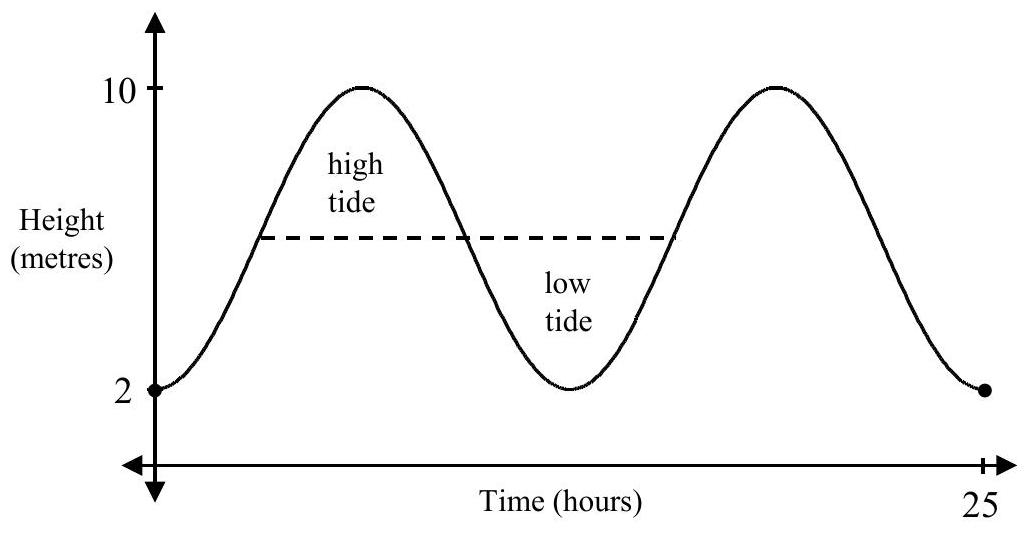
\includegraphics[max width=\textwidth, alt={}, center]{f67fedaf-ea11-42ad-a16e-f30d2fcf2bd3-074_534_1034_470_191}\\
a) What is the average height of the water?\\
b) What is the period of the graph above?

Explain what the period represents in this situation.

\section*{Solution}
a) 6 metres □ 1 mark\\
b) Period $=\frac{25}{2}$ 1 mark for period

$$
=12.5 \text { hours }
$$

The period represents the time to complete one cycle of tidal levels in the Bay of Fundy.

1 mark for explanation\\
2 marks

Given the graph of $y=f(x)$, sketch the graph of $y=\sqrt{f(x)}$.\\
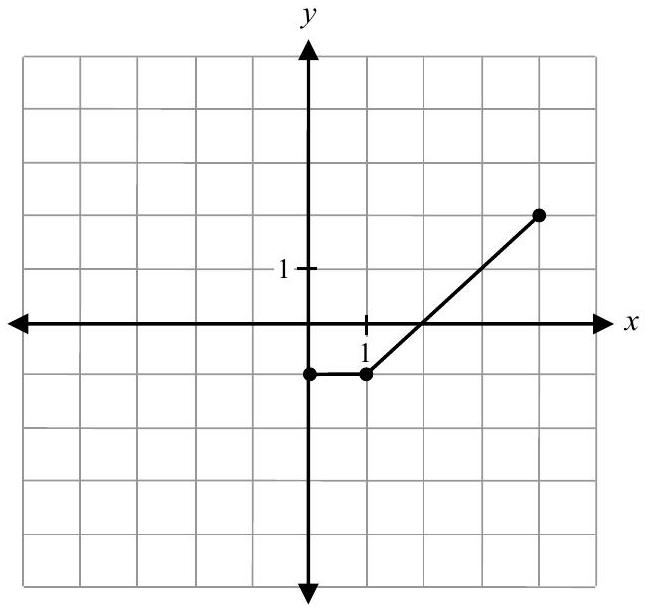
\includegraphics[max width=\textwidth, alt={}, center]{f67fedaf-ea11-42ad-a16e-f30d2fcf2bd3-075_611_648_483_171}

\section*{Solution}
\begin{center}
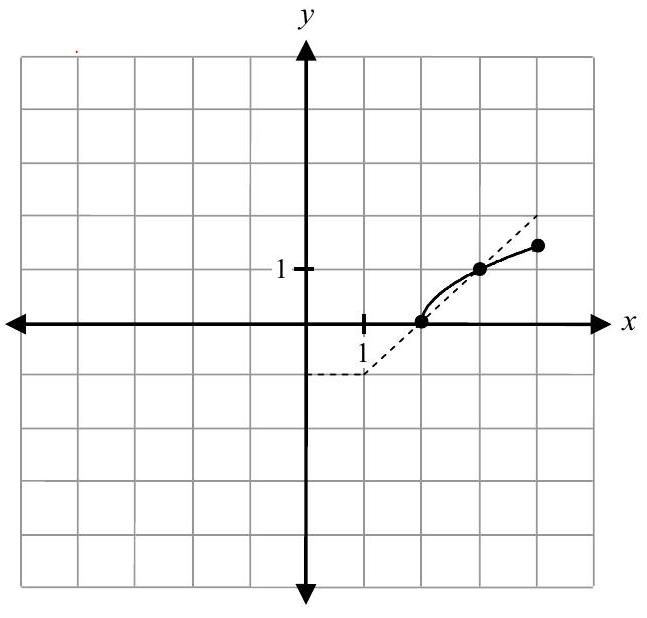
\includegraphics[max width=\textwidth, alt={}]{f67fedaf-ea11-42ad-a16e-f30d2fcf2bd3-075_618_647_1241_189}
\end{center}

1 mark for restricting the domain\\
$\frac{1}{2}$ mark for graph above $y=f(x)$ over the range $[0,1]$\\
$\frac{1}{2}$ mark for graph below $y=f(x)$ over the range $[1,2]$\\
2 marks

When $P(x)$ is divided by $x-3$, it has a quotient of $2 x^{2}+x-6$ and a remainder of 4 .\\
Determine $P(x)$.

\section*{Solution}
$P(x)=(x-3)\left(2 x^{2}+x-6\right)+4$\\
1 mark for polynomial $P(x)$\\
or\\
1 mark\\
$P(x)=2 x^{3}-5 x^{2}-9 x+22$

Identify the domain and range of the following function:

$$
f(x)=\frac{3}{x^{2}+1}
$$

\section*{Solution}
\begin{center}
\begin{tabular}{cc}
Domain: $\{x \in \mathbb{R}\}$ & 1 mark for domain \\
or &  \\
$(-\infty, \infty)$ & 1 mark for range \\
Range: $\{y \in \mathbb{R} \mid 0<y \leq 3\}$ & $\mathbf{2}$ marks \\
or &  \\
\end{tabular}
\end{center}

Evaluate:

$$
\csc \left(\frac{11 \pi}{6}\right)+\sin ^{2}\left(-\frac{3 \pi}{4}\right)+\cos \left(\frac{23 \pi}{3}\right)
$$

\section*{Solution}
$=(-2)+\left(-\frac{\sqrt{2}}{2}\right)^{2}+\frac{1}{2}$\\
1 mark for $\csc \left(\frac{11 \pi}{6}\right)\left(\frac{1}{2}\right.$ mark for quadrant, $\frac{1}{2}$ mark for value $)$\\
$=-2+\frac{1}{2}+\frac{1}{2}$\\
1 mark for $\sin ^{2}\left(-\frac{3 \pi}{4}\right)(1 / 2$ mark for quadrant, $1 / 2$ mark for value $)$\\
$=-1$\\
1 mark for $\cos \left(\frac{23 \pi}{3}\right)\left(\frac{1}{2}\right.$ mark for quadrant, $1 / 2$ mark for value $)$

Evaluate the coefficient of the term containing $x^{3}$ in the expansion of $(1+x)^{7}$.\\
Justify your answer.

\section*{Solution}
\section*{Method 1}
\begin{center}
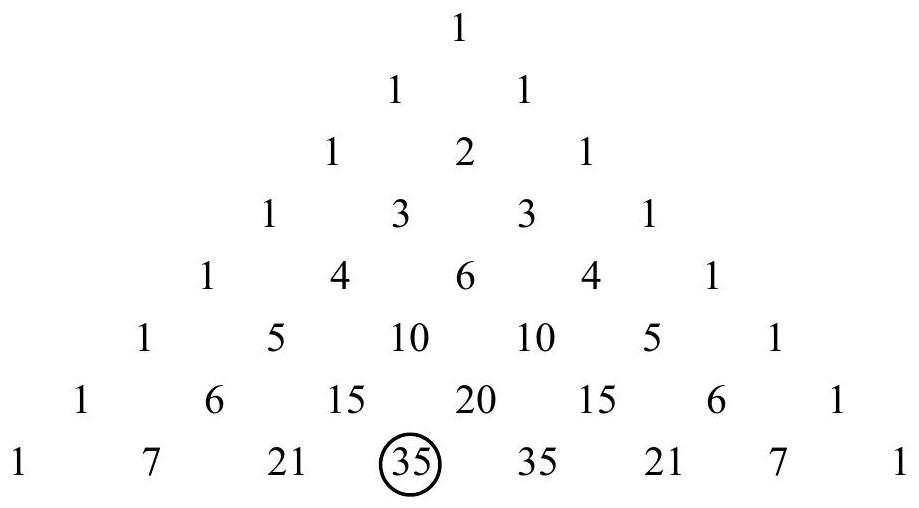
\includegraphics[max width=\textwidth, alt={}]{f67fedaf-ea11-42ad-a16e-f30d2fcf2bd3-079_508_919_717_171}
\end{center}

1 mark for justification

The coefficient of $x^{3}$ is 35 .\\
1 mark for identifying coefficient

\section*{2 marks}
\section*{Method 2}
$$
\begin{aligned}
t_{4} & ={ }_{7} C_{3}(1)^{4}(x)^{3} \\
{ }_{7} C_{3} & =\frac{7!}{3!4!} \\
& =\frac{7 \cdot \varnothing \cdot 5 \cdot 4!}{3!4!} \\
& =35
\end{aligned}
$$

1 mark for justification

1 mark for evaluating coefficient

The coefficient of $x^{3}$ is 35 .

Which of the following equations could be solved without the use of logarithms?\\
Without actually solving the problem, explain your choice.

$$
4^{x}=10^{3 x+1} \quad \text { or } \quad\left(\frac{1}{3}\right)^{2 x+1}=27^{4 x-1}
$$

\section*{Solution}
$\left(\frac{1}{3}\right)^{2 x+1}=27^{4 x-7}$ can be solved without the use of logarithms because $\frac{1}{3}$ and 27 can both be changed to a base of 3 .

1 mark for explanation\\
1 mark

Sketch the graph of $y=x^{3}+x^{2}-5 x+3$ given that one of the $x$-intercepts is 1 .\\
Identify the $x$-intercepts and $y$-intercept.

\section*{Solution}
$$
x=1
$$

\begin{center}
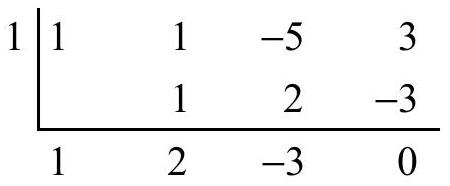
\includegraphics[max width=\textwidth, alt={}]{f67fedaf-ea11-42ad-a16e-f30d2fcf2bd3-081_186_450_745_253}
\end{center}

$$
1 \text { mark for synthetic division }
$$

$$
y=(x-1)\left(x^{2}+2 x-3\right)
$$

$$
y=(x-1)(x+3)(x-1)
$$

$$
y=(x+3)(x-1)^{2}
$$

1 mark for identifying the factors\\
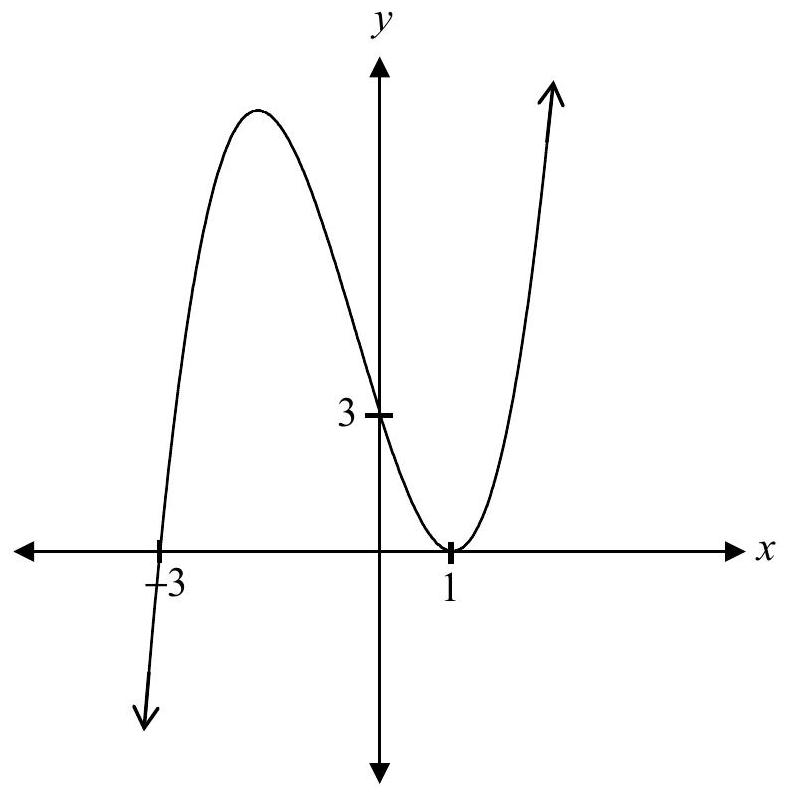
\includegraphics[max width=\textwidth, alt={}, center]{f67fedaf-ea11-42ad-a16e-f30d2fcf2bd3-081_796_791_1325_146}

2 marks for graph ( $\frac{1}{2}$ mark for $x$-intercepts, $\frac{1}{2}$ mark for multiplicity, $\frac{1}{2}$ mark for $y$-intercept, $\frac{1}{2}$ mark for end behaviour)

\section*{4 marks}
If $f(x)=\frac{1}{x-2}$ and $g(x)=x-2$, what is the domain of $f(x) \cdot g(x)$ ?

\section*{Solution}
$f(x)=\frac{1}{x-2} \quad g(x)=x-2$\\
Domain: $x \in \mathbb{R}, x \neq 2 \quad$ Domain: $x \in \mathbb{R}$

Domain of $f(x) \cdot g(x):\{x \in \mathbb{R} \mid x \neq 2\} \quad 1$ mark for domain of $f(x) \cdot g(x)$\\
1 mark

Given $f(x)=(x+1)^{2}$ for $x \leq-1$, write the equation of $y=f^{-1}(x)$.

\section*{Solution}
\section*{Method 1}
$$
\begin{aligned}
& y=(x+1)^{2} \\
& x=(y+1)^{2} \\
& y= \pm \sqrt{x}-1
\end{aligned}
$$

1 mark for inverse\\
$\frac{1}{2}$ mark for solving for $y$

Since the domain of $f(x)$ is $x \leq-1$,\\
the range of the inverse is $y \leq-1$.

$$
\begin{aligned}
\therefore y & =-\sqrt{x}-1 \\
f^{-1}(x) & =-\sqrt{x}-1
\end{aligned}
$$

$\frac{1}{2}$ mark for rejecting $y=\sqrt{x}$

\section*{2 marks}
\section*{Method 2}
(where\\
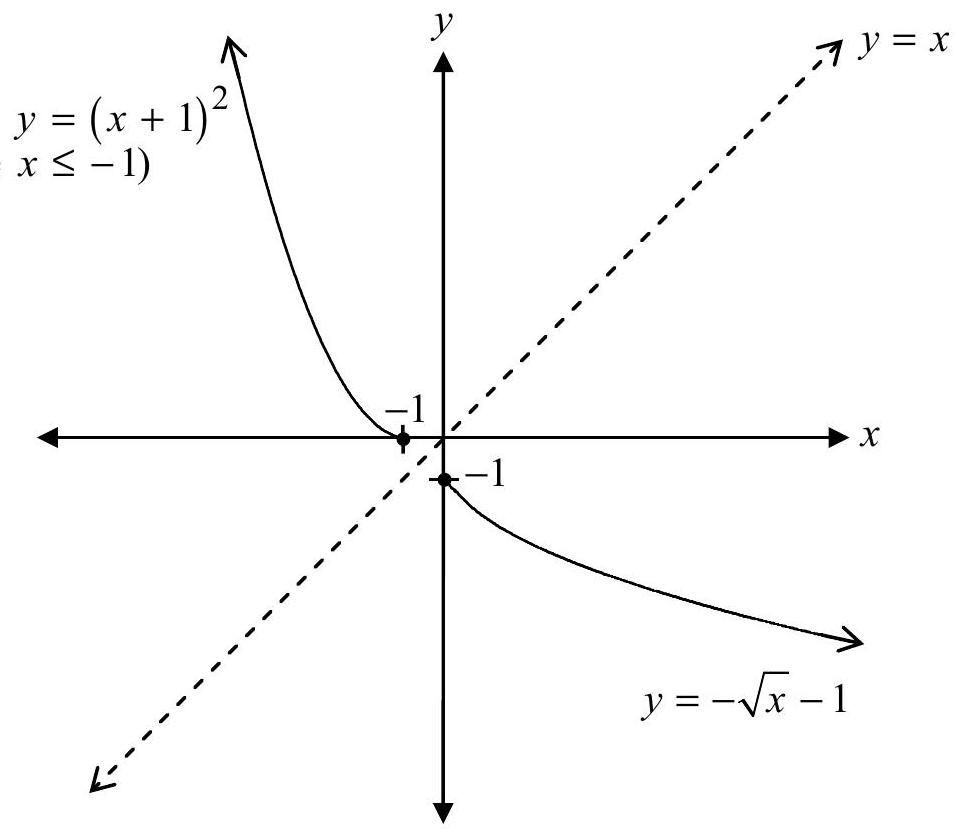
\includegraphics[max width=\textwidth, alt={}, center]{f67fedaf-ea11-42ad-a16e-f30d2fcf2bd3-083_835_957_1531_262}

1 mark for reflection over the line $y=x$

1 mark for correct equation\\
2 marks

Sketch a graph of at least one period of the function $y=5 \sin [\pi(x+1)]$.\\
Clearly indicate the $x$-intercepts.

\section*{Solution}
$b=\pi$\\
∴ period $=\frac{2 \pi}{\pi}=2$\\
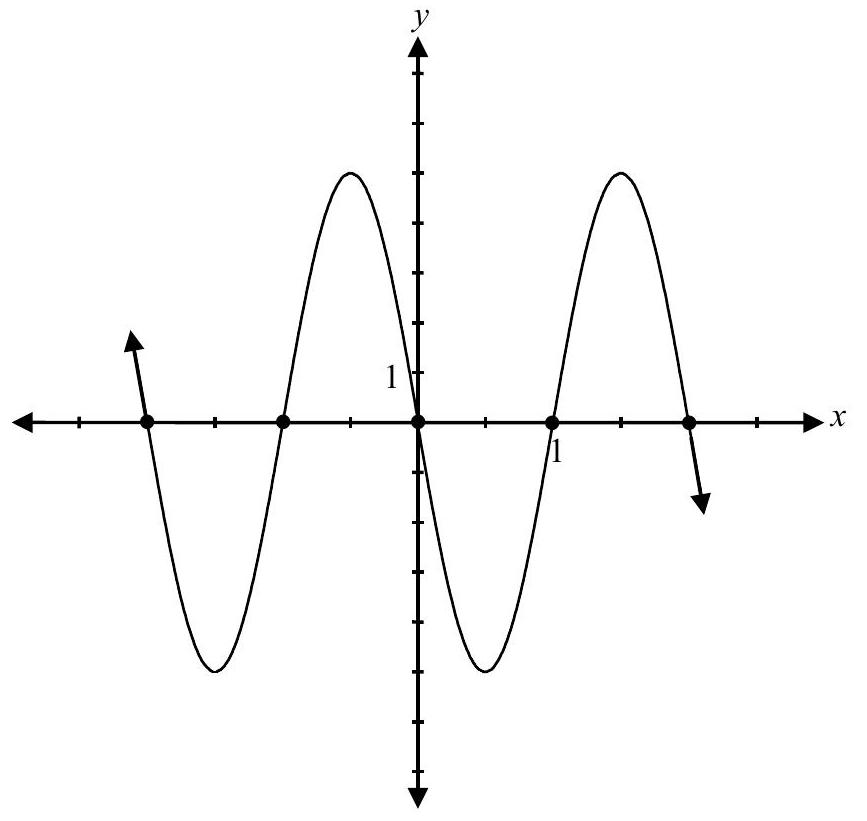
\includegraphics[max width=\textwidth, alt={}, center]{f67fedaf-ea11-42ad-a16e-f30d2fcf2bd3-084_821_867_827_156}

1 mark for amplitude\\
1 mark for horizontal shift\\
1 mark for period\\
1 mark for clearly indicating at least two $x$-intercepts consistent with graph

4 marks

Sketch the graph of the following function:

$$
f(x)=\frac{x-2}{(2 x-3)(x-2)}
$$

\section*{Solution}
$$
\begin{aligned}
f(x) & =\frac{x-2}{(2 x-3)(x-2)} \\
& =\frac{1}{2 x-3} \text { with a point of discontinuity at } x=2
\end{aligned}
$$

point of discontinuity: $f(2)=1$\\
∴ there is a point of discontinuity at $(2,1)$

$$
y \text {-intercept: } \begin{aligned}
f(0) & =\frac{0-2}{(2(0)-3)(0-2)} \\
& =-\frac{2}{6} \\
& =-\frac{1}{3}
\end{aligned}
$$

\begin{center}
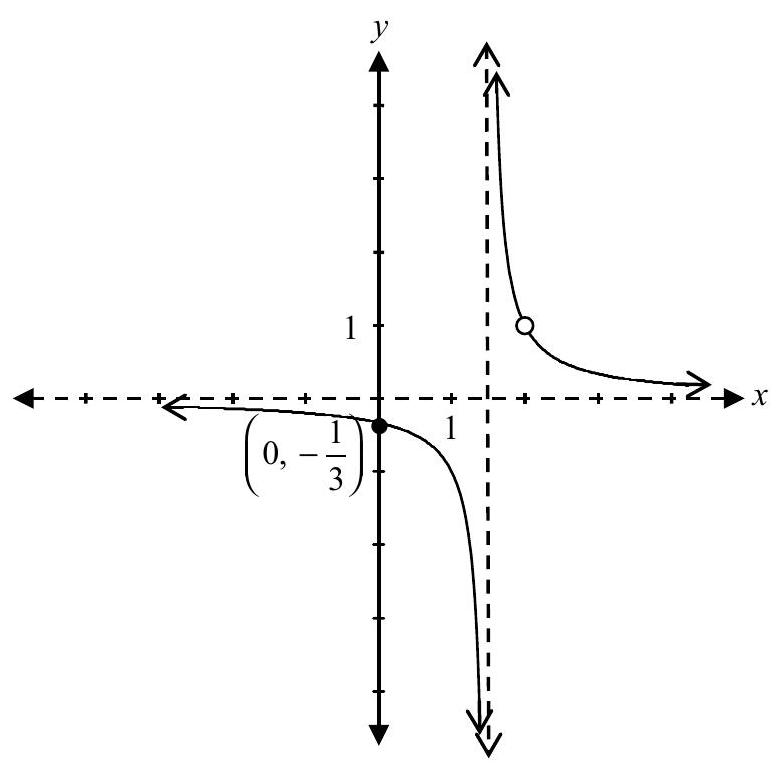
\includegraphics[max width=\textwidth, alt={}]{f67fedaf-ea11-42ad-a16e-f30d2fcf2bd3-085_770_776_687_1158}
\end{center}

1 mark for horizontal asymptote at $y=0$\\
1 mark for vertical asymptote at $x=\frac{3}{2}$\\
$\frac{1}{2}$ mark for graph left of vertical asymptote\\
$\frac{1}{2}$ mark for graph right of vertical asymptote\\
1 mark for point of discontinuity at $(2,1)$; ( $1 / 2$ mark for $x=2, \frac{1}{2}$ mark for $y=1$ )

\section*{4 marks}
Convert $-\frac{13 \pi}{5}$ to degrees.

\section*{Solution}
$$
\begin{aligned}
& -\frac{13 \pi}{5} \times \frac{180^{\circ}}{\pi} \\
& -468^{\circ}
\end{aligned}
$$


\includegraphics[max width=\textwidth, alt={}, center]{f67fedaf-ea11-42ad-a16e-f30d2fcf2bd3-086_123_218_743_674}\\
a) From a group of 9 people, in how many ways can you select a committee of 4 members?\\
b) From a group of 9 people, in how many ways can you select a president, a vice president, a secretary, and a treasurer?\\
c) Explain why the answers in a) and b) are different.

\section*{Solution}
a) ${ }_{9} C_{4}=126$ ways

1 mark for ${ }_{9} C_{4}$\\
□\\
1 mark\\
b) ${ }_{9} P_{4}=3024$ ways

1 mark for ${ }_{9} P_{4}$\\
□\\
1 mark\\
c) Part a) is a combination because the order does not matter; part b) is a permutation because committee members have specific roles.\\
□\\
1 mark

A population of 500 bacteria will triple in 20 hours.\\
Using the formula given below,\\
$A=P e^{r t}$\\
$A=$ population after $t$ hours\\
$P=$ initial population\\
$r=$ rate of growth\\
$t=$ time in hours\\
a) Determine the rate of growth, $r$.\\
b) Determine how many hours it will take for the initial population to double with the same rate of growth.

\section*{Solution}
a)

$$
\begin{aligned}
1500 & =500 e^{r(20)} & & 1 / 2 \text { mark for substitution } \\
3 & =e^{20 r} & & \\
\ln 3 & =\ln e^{20 r} & & 1 / 2 \text { mark for applying logarithms } \\
\ln 3 & =20 r \cdot \ln e & & 1 / 2 \text { mark for power rule } \\
r & =\frac{\ln 3}{20} & & \\
r & =0.054930614 & & 1 / 2 \text { mark for evaluating quotient of logarithms }
\end{aligned}
$$

b)

$$
\begin{aligned}
1000 & =500 e^{0.054930614 t} & & 1 / 2 \text { mark for substitution } \\
2 & =e^{0.054930614 t} & & \\
\ln 2 & =\ln e^{0.054930614 t} & & 1 / 2 \text { mark for applying logarithms } \\
\ln 2 & =0.054930614 t \cdot \ln e & & 1 / 2 \text { mark for power rule } \\
t & =\frac{\ln 2}{0.054930614} & & \\
t & =12.619 \text { hours } & & 1 / 2 \text { mark for evaluating quotient of logarithms }
\end{aligned}
$$

2 marks

Talla incorrectly solved the following trigonometric equation:\\
Solve: $2 \sec x-5=0 ; 0^{\circ} \leq x \leq 360^{\circ}$.\\
Talla's work:\\
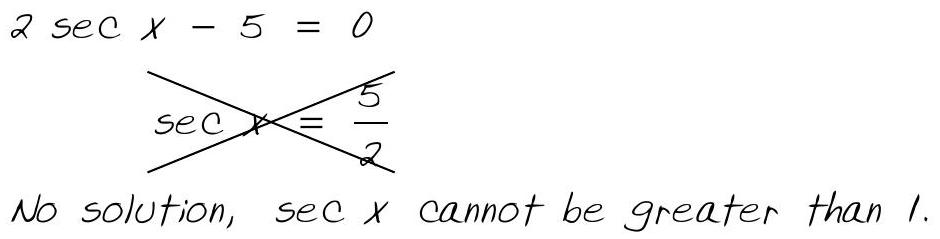
\includegraphics[max width=\textwidth, alt={}, center]{f67fedaf-ea11-42ad-a16e-f30d2fcf2bd3-089_239_940_623_515}\\
a) Explain her error.\\
b) Determine the correct solution.

\section*{Solution}
a) Talla incorrectly stated that sec $x$ cannot be greater than 1 .

The value of $\cos x$ cannot be greater than 1 .\\
b) $\quad \sec x=\frac{5}{2}$

$$
\begin{aligned}
\cos x & =\frac{2}{5} \\
x_{r} & =66.421821 \\
x & =66.422^{\circ} \\
x & =293.578^{\circ}
\end{aligned}
$$

1 mark for reciprocal

1 mark for solving for $x$ ( $\frac{1}{2}$ mark for each value of $x$ )

2 marks

Simplify the 6th term in the expansion of:

$$
\left(2 x-\frac{3}{x^{2}}\right)^{10}
$$

\section*{Solution}
$$
\begin{aligned}
t_{6} & ={ }_{10} C_{5}(2 x)^{5}\left(-\frac{3}{x^{2}}\right)^{5} \\
& =252\left(32 x^{5}\right)\left(-\frac{243}{x^{10}}\right) \\
& =-1959552 x^{-5}
\end{aligned}
$$

2 marks (1 mark for ${ }_{10} C_{5}, \frac{1}{2}$ mark for each consistent factor)

1 mark for simplification ( $\frac{1}{2}$ mark for coefficient, $\frac{1}{2}$ mark for exponent)

Determine the arc length subtended by a central angle if the diameter is 19 cm and the central angle is 1.6 radians.

\section*{Solution}
$$
\begin{aligned}
& s=\theta r \\
& s=(1.6)(9.5) \\
& s=15.2 \mathrm{~cm}
\end{aligned}
$$

Solve the following equation algebraically for $x$, where $0 \leq x \leq 2 \pi$.

$$
2 \cos ^{2} x=-3 \sin x
$$

\section*{Solution}
$$
\begin{aligned}
2\left(1-\sin ^{2} x\right) & =-3 \sin x \\
2-2 \sin ^{2} x & =-3 \sin x \\
0 & =2 \sin ^{2} x-3 \sin x-2 \\
0 & =(2 \sin x+1)(\sin x-2) \\
\sin x & =-\frac{1}{2} \quad \text { No Solution } \\
x & =\frac{7 \pi}{6} \\
x & =\frac{11 \pi}{6}
\end{aligned}
$$

1 mark for identity

1 mark for solving for $\sin x$\\
1 mark for indicating no solution\\
1 mark for solving for $x\left(\frac{1}{2}\right.$ mark for each value)

4 marks

In how many different ways can you arrange the letters in the word VOLLEYBALL? State your answer as a factorial.

\section*{Solution}
$\frac{10!}{4!}$

$$
1 \text { mark }
$$

Note(s):

\begin{itemize}
  \item award full marks for 151200
\end{itemize}

Is $(x-2)$ a factor of the polynomial $p(x)=-x^{4}-3 x^{3}+11 x^{2}+3 x-10$ ?\\
Justify your response.

\section*{Solution}
\section*{Method 1}
$$
\begin{aligned}
p(2) & =-(2)^{4}-3(2)^{3}+11(2)^{2}+3(2)-10 \\
& =-16-24+44+6-10 \\
& =0
\end{aligned}
$$

$\frac{1}{2}$ mark for $p(2)$\\
1 mark for the remainder theorem

The remainder is zero, so $(x-2)$ is a factor.\\
$\frac{1}{2}$ mark for justification

\section*{2 marks}
\section*{Method 2}
\begin{center}
\begin{tabular}{r|rrrrr}
2 & -1 & -3 & 11 & 3 & -10 \\
 & $\downarrow$ & -2 & -10 & 2 & 10 \\
\hline
 & -1 & -5 & 1 & 5 & $\lfloor 0$ \\
\hline
\end{tabular}
\end{center}

$\frac{1}{2}$ mark for $x=2$

1 mark for synthetic division (or for any equivalent strategy)\\
$\frac{1}{2}$ mark for justification\\
The remainder is zero, so $(x-2)$ is a factor.

\section*{2 marks}
\section*{Method 3}
I entered $y=-x^{4}-3 x^{3}+11 x^{2}+3 x-10$ into my calculator and located the zeroes.\\
$x=2$ was a zero, which means $(x-2)$ is a factor.\\
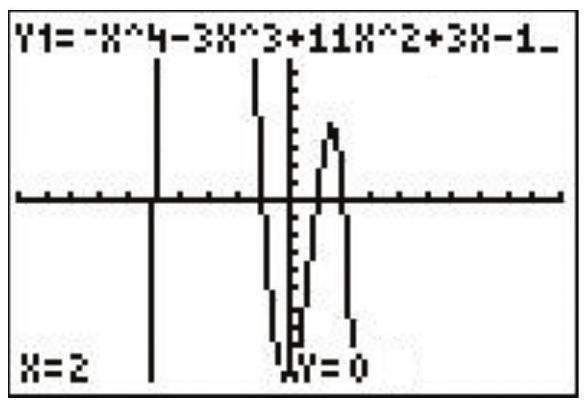
\includegraphics[max width=\textwidth, alt={}, center]{f67fedaf-ea11-42ad-a16e-f30d2fcf2bd3-094_405_585_2161_305}

1 mark for graphing calculator method

1 mark for relating the zeroes to the factors

2 marks

Determine the period of the sinusoidal function $y=\frac{1}{2} \sin \left(\frac{1}{3} x\right)$.\\
State your answer in radians.

\section*{Solution}
$$
\begin{aligned}
& p=\frac{2 \pi}{|\mathrm{~b}|} \\
& p=\frac{2 \pi}{\left|\frac{1}{3}\right|}
\end{aligned}
$$

$p=6 \pi$ or $p=18.85$

$$
\begin{aligned}
& 1 / 2 \text { mark for correct value of } b \\
& 1 / 2 \text { mark for period consistent with } b
\end{aligned}
$$

1 mark

The domain of $f(x)$ is $x \leq 2$. The domain of $g(x)$ is $x \geq-7$.\\
State the domain of $f(x)+g(x)$.\\
Justify your answer.

\section*{Solution}
Both $f(x)$ and $g(x)$ have restricted domains, so both domains need to be considered.\\
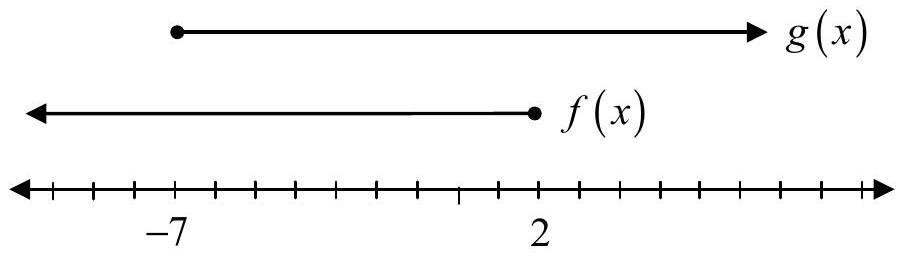
\includegraphics[max width=\textwidth, alt={}, center]{f67fedaf-ea11-42ad-a16e-f30d2fcf2bd3-096_259_906_915_184}

The solution is the intersection of the two domains.

$$
\{x \mid x \in \mathbb{R},-7 \leq x \leq 2\} \quad \text { or } \quad[-7,2]
$$

1 mark for justification\\
1 mark for domain\\
2 marks

Prove the identity below for all permissible values of $\theta$.

$$
\frac{1}{1+\cos \theta}=\csc ^{2} \theta-\frac{\cot \theta}{\sin \theta}
$$

\section*{Solution}
\section*{Method 1}
\begin{center}
\begin{tabular}{|l|l|}
\hline
Left-Hand Side & Right-Hand Side \\
\hline
\multirow[t]{8}{*}{\(
\frac{1}{1+\cos \theta}
\)} & \( \csc ^{2} \theta-\frac{\cot \theta}{\operatorname{Lin}} \) \\
\hline
 & $\frac{1}{\sin ^{2} \theta}-\frac{\frac{\cos \theta}{\sin \theta}}{\sin \theta}$ \\
\hline
 & \( \begin{aligned} & \frac{1}{\sin ^{2} \theta}-\frac{\cos \theta}{\sin \theta} \cdot \frac{1}{\sin \theta} \\ & \frac{1}{\sin ^{2} \theta}-\frac{\cos \theta}{\sin ^{2} \theta} \end{aligned} \) \\
\hline
 &  \\
\hline
 & $\frac{1-\cos \theta}{\sin ^{2} \theta}$ \\
\hline
 & $\frac{1-\cos \theta}{1-\cos ^{2} \theta}$ \\
\hline
 & $\frac{1-\cos \theta}{(1-\cos \theta)(1+\cos \theta)}$ \\
\hline
 & $\frac{1}{1+\cos \theta}$ \\
\hline
\end{tabular}
\end{center}

1 mark for correct substitution of identities

1 mark for algebraic strategies

1 mark for logical process to prove an identity

3 marks

\section*{Solution}
\section*{Method 2}
\begin{center}
\begin{tabular}{|l|l|l|}
\hline
Left-Hand Side & Right-Hand Side &  \\
\hline
\multicolumn{3}{|l|}{\begin{tabular}{l}
\( \frac{1}{1+\cos \theta}(1-\cos \theta) \) \\
$\csc ^{2} \theta-\frac{\cot \theta}{\sin \theta}$ \\
1 mark for algebraic strategies \\
$\frac{1-\cos \theta}{1-\cos ^{2} \theta}$ \\
\end{tabular}} \\
\hline
$\frac{1-\cos \theta}{\sin ^{2} \theta}$ &  & 1 mark for correct substitution of identities \\
\hline
\( \csc ^{2} \theta-\frac{\cos \theta}{\sin \theta} \cdot \frac{1}{\sin \theta} \) &  & 1 mark for logical process to prove an identity \\
\hline
$\csc ^{2} \theta-\frac{\cot \theta}{\sin \theta}$ &  & 3 marks \\
\hline
\end{tabular}
\end{center}

Explain how the end behaviours of the graphs of polynomial functions with an even degree and with an odd degree are different.

\section*{Solution}
When the degree is odd, the end behaviour is in opposite directions. When the degree is even, the end behaviour is in the same direction.

Given the graphs of $f(x)$ and $g(x)$, sketch the graph of $g(x)-f(x)$.\\
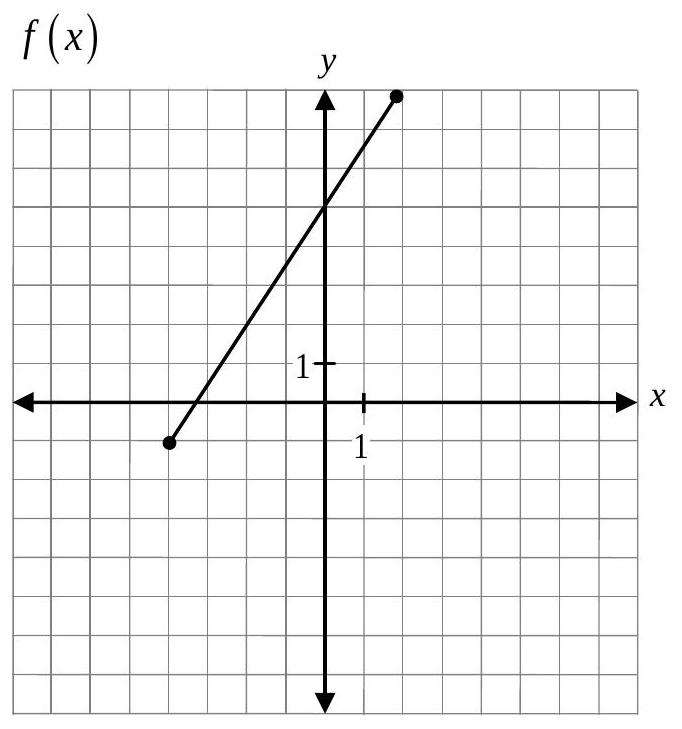
\includegraphics[max width=\textwidth, alt={}, center]{f67fedaf-ea11-42ad-a16e-f30d2fcf2bd3-100_729_682_485_197}\\
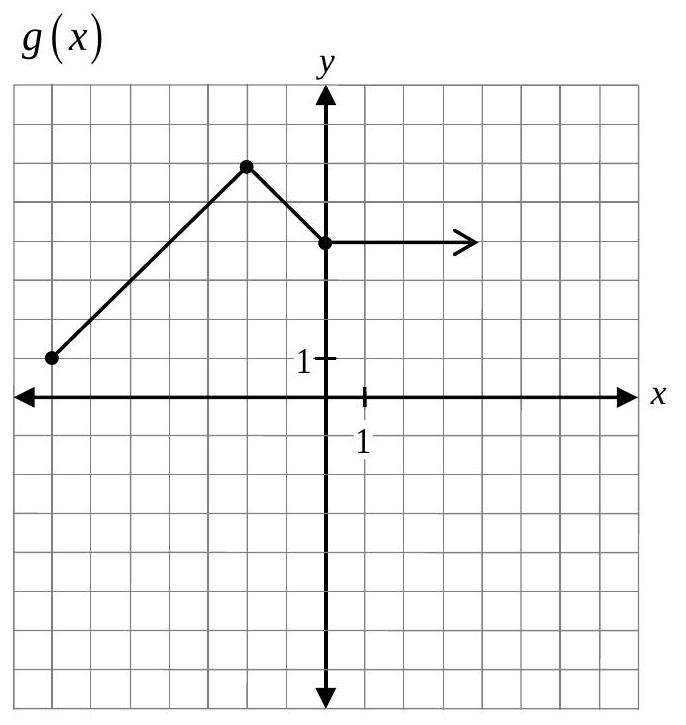
\includegraphics[max width=\textwidth, alt={}, center]{f67fedaf-ea11-42ad-a16e-f30d2fcf2bd3-100_725_686_485_1020}

\section*{Solution}
\begin{center}
\begin{tabular}{c|c|c|c}
$x$ & $g(x)$ & $f(x)$ & $(g-f)(x)$ \\
\hline
-4 & 4 & -1 & 5 \\
-2 & 6 & 2 & 4 \\
0 & 4 & 5 & -1 \\
2 & 4 & 8 & -4 \\
\end{tabular}
\end{center}

1 mark for subtraction of $g(x)-f(x)$\\
1 mark for restricting domain on graph\\
2 marks

$$
g(x)-f(x)
$$

\begin{center}
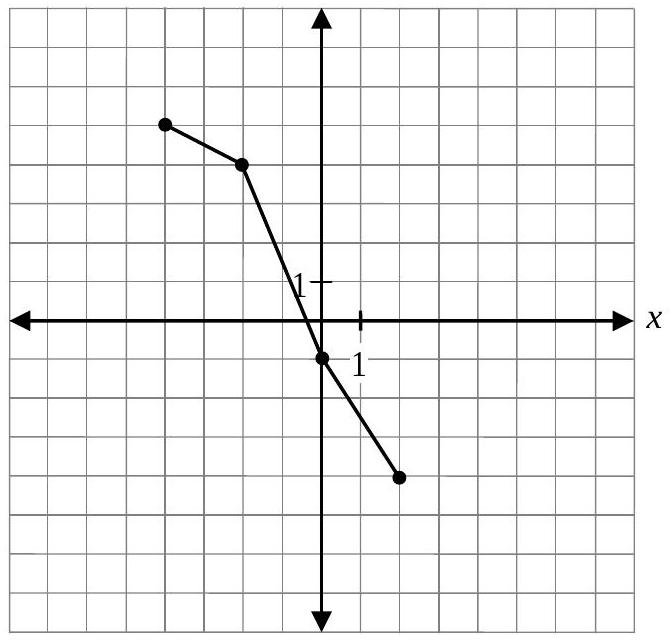
\includegraphics[max width=\textwidth, alt={}]{f67fedaf-ea11-42ad-a16e-f30d2fcf2bd3-100_642_671_1357_1035}
\end{center}

Given $f(x)=-3 x+7$, evaluate $f^{-1}(-2)$.

\section*{Solution}
$$
\begin{aligned}
\text { Let } y & =f(x) & & \\
f(x) & =-3 x+7 & & \\
y & =-3 x+7 & & 1 \text { mark for switching } x \text { and } y \\
x & =-3 y+7 & & \\
x-7 & =-3 y & & \\
y & =\frac{x-7}{-3} & & 1 / 2 \text { mark for } f^{-1}(x) \\
f^{-1}(x) & =\frac{x-7}{-3} & & \\
f^{-1}(-2) & =\frac{-2-7}{-3} & & 1 / 2 \text { mark for } f^{-1}(-2) \\
f^{-1}(-2) & =3 & & \mathbf{2} \text { marks }
\end{aligned}
$$

How many terms are there in the expansion of $\left(x^{12}+3\right)^{10} ?$\\
a) 9\\
b) 10\\
c) 11\\
d) 12

Question 17

A co-terminal angle for $\theta=\frac{11 \pi}{3}$ in the domain $-2 \pi \leq \theta \leq 0$ would be:\\
a) $-\frac{5 \pi}{3}$\\
b) $-\frac{\pi}{3}$\\
c) $\frac{\pi}{3}$\\
d) $\frac{5 \pi}{3}$

Question 18

The $x$-intercept of the graph of $y=3^{x}-1$ is:\\
a) -1\\
b) 0\\
c) 1\\
d) 2

If ${ }_{n} C_{5}={ }_{n} C_{3}$, the value of $n$ must be:\\
a) 3\\
b) 5\\
c) 8\\
d) 15

Question 20

What is the domain of the function $f(x)=\sqrt{-(x+1)}$ ?\\
a) $\{x \mid x \in \mathbb{R}, x \neq-1\}$\\
b) $\{x \mid x \in \mathbb{R}, x \geq-1\}$\\
c) $\{x \mid x \in \mathbb{R}, x \leq-1\}$\\
d) $\{x \mid x \in \mathbb{R}\}$

Question 21

Identify a non-permissible value of $x$ for the expression $\frac{1}{\cos 2 x}$.\\
a) 0\\
b) $\frac{\pi}{4}$\\
c) $\frac{\pi}{2}$\\
d) $\pi$

The expression $2 \log x-\frac{1}{3} \log y$ as a single logarithm is:\\
a) $\log \frac{x^{2}}{\sqrt[3]{y}}$\\
b) $\quad \log \frac{2 x}{3 y}$\\
c) $-\log x^{2} \sqrt[3]{y}$\\
d) $\log \left(x^{2}-\sqrt[3]{y}\right)$

Question 23

The point $\mathrm{P}(\theta)$ lies on the unit circle. What are the coordinates of the point if $\theta=300^{\circ}$ ?\\
a) $\left(\frac{1}{2}, \frac{\sqrt{3}}{2}\right)$\\
b) $\left(-\frac{1}{2}, \frac{\sqrt{3}}{2}\right)$\\
c) $\left(\frac{\sqrt{3}}{2},-\frac{1}{2}\right)$\\
d) $\left(\frac{1}{2},-\frac{\sqrt{3}}{2}\right)$

What is the degree of the polynomial function represented by the graph below?\\
a) 2\\
b) 3\\
c) 4\\
d) 5\\
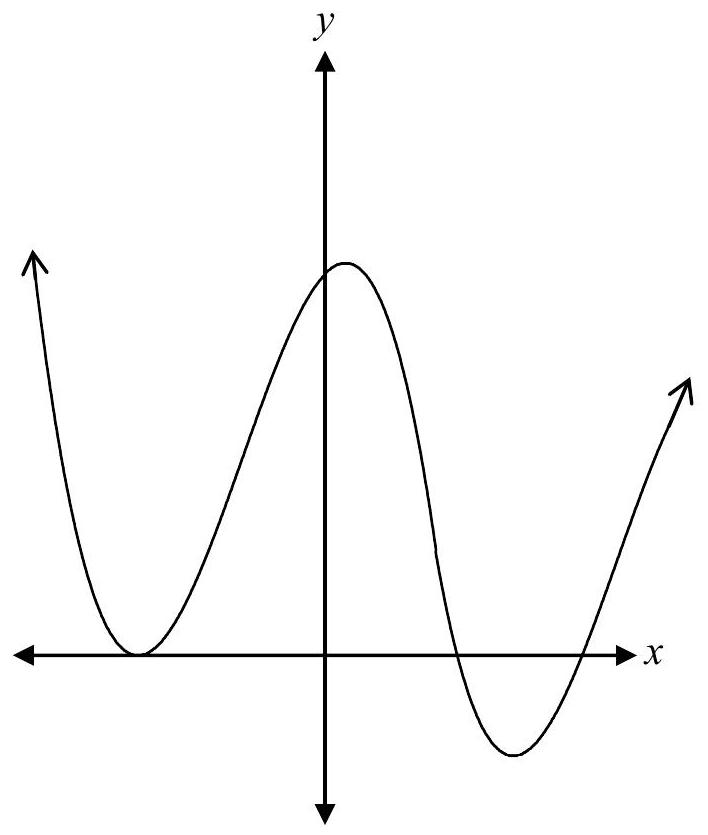
\includegraphics[max width=\textwidth, alt={}, center]{f67fedaf-ea11-42ad-a16e-f30d2fcf2bd3-105_835_708_485_1052}

When the point $(-4,-3)$ is reflected over the line $y=x$, the coordinates of the new point are:\\
а) $(-3,-4)$\\
b) $(3,4)$\\
c) $(4,-3)$\\
d) $(-4,3)$

Sketch the graphs of:\\
a) $y=\left(\frac{1}{4}\right)^{x}$\\
b) $y=2\left(\frac{1}{4}\right)^{x}$\\
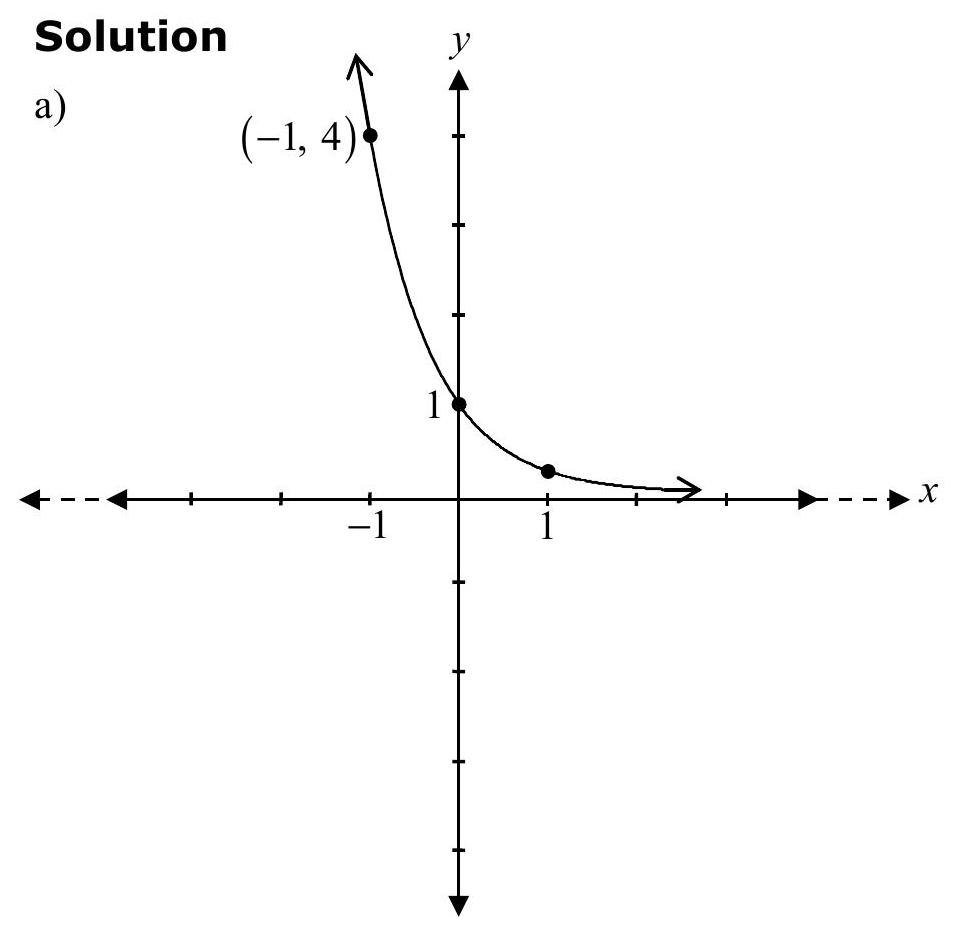
\includegraphics[max width=\textwidth, alt={}, center]{f67fedaf-ea11-42ad-a16e-f30d2fcf2bd3-106_933_962_715_143}\\
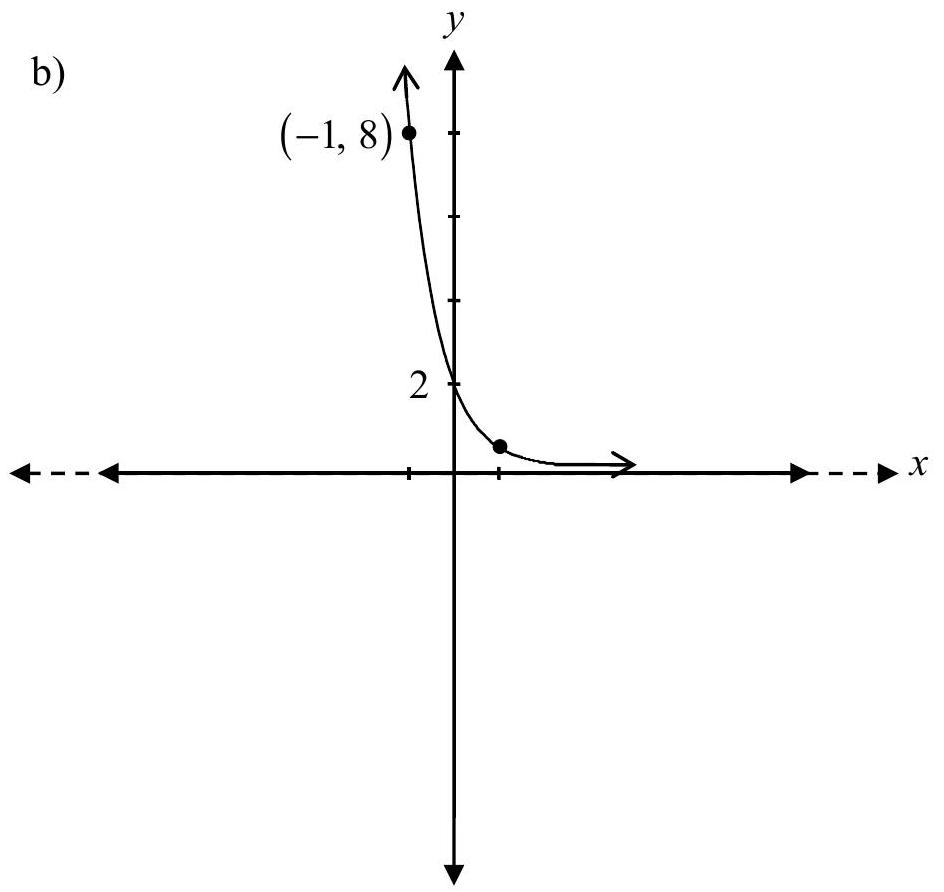
\includegraphics[max width=\textwidth, alt={}, center]{f67fedaf-ea11-42ad-a16e-f30d2fcf2bd3-106_892_944_1710_146}\\
$\frac{1}{2}$ mark for decreasing exponential function\\
$\frac{1}{2}$ mark for $y$-intercept $(0,1)$\\
$\frac{1}{2}$ mark for consistent point of an exponential function\\
$\frac{1}{2}$ mark for horizontal asymptote at $y=0$

2 marks

1 mark for a vertical stretch by a factor of 2 of the graph consistent with a)

1 mark

Determine all of the zeroes of the function $p(x)=x^{3}-5 x^{2}-2 x+24$, given one of the factors of $p(x)$ is $(x-3)$.

\section*{Solution}
$0=x^{3}-5 x^{2}-2 x+24$

\begin{center}
\begin{tabular}{c|cccc}
3 & 1 & -5 & -2 & 24 \\
 & $\downarrow$ & 3 & -6 & -24 \\
\hline
 & 1 & -2 & -8 & 0 \\
\hline
\end{tabular}
\end{center}

$\frac{1}{2}$ mark for $x=3$\\
1 mark for synthetic division (or for any equivalent strategy)

$$
\begin{aligned}
& x^{2}-2 x-8=0 \\
& (x-4)(x+2)=0 \\
& \text { zeroes: } 3,4,-2
\end{aligned}
$$

$\frac{1}{2}$ mark for consistent zeroes

Given the graph of $f(x)$,\\
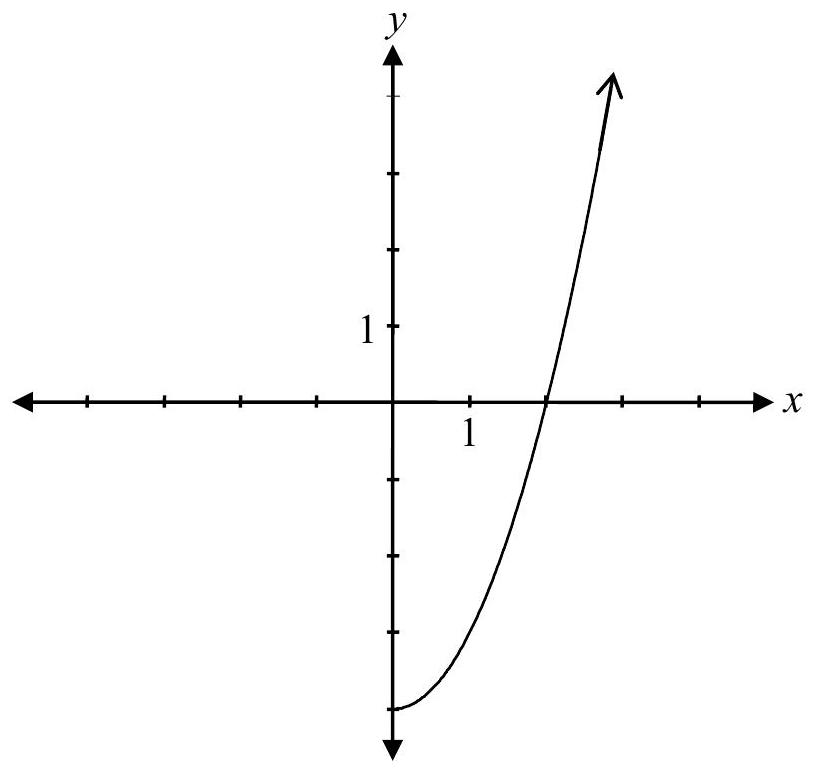
\includegraphics[max width=\textwidth, alt={}, center]{f67fedaf-ea11-42ad-a16e-f30d2fcf2bd3-108_768_813_468_178}\\
sketch the graph of $y=\sqrt{f(x)}$.

\section*{Solution}
\begin{center}
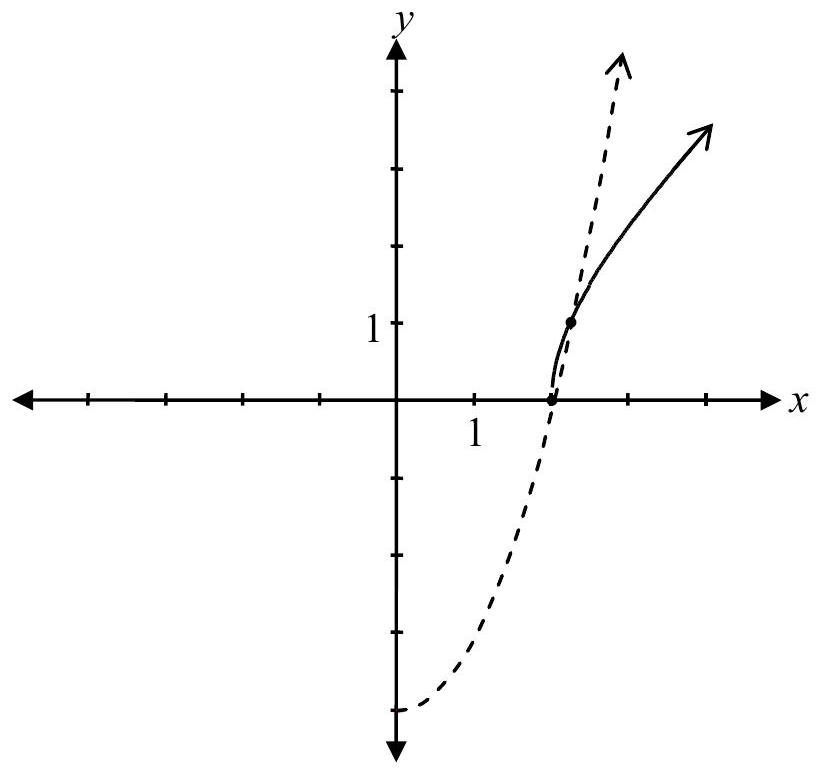
\includegraphics[max width=\textwidth, alt={}]{f67fedaf-ea11-42ad-a16e-f30d2fcf2bd3-108_773_817_1533_176}
\end{center}

1 mark for restricting domain\\
$\frac{1}{2}$ mark for shape between invariant points\\
$\frac{1}{2}$ mark for shape to the right of the invariant points

2 marks

Sketch the graph of at least one period of the function $y=-2 \sin (4 x)$.\\
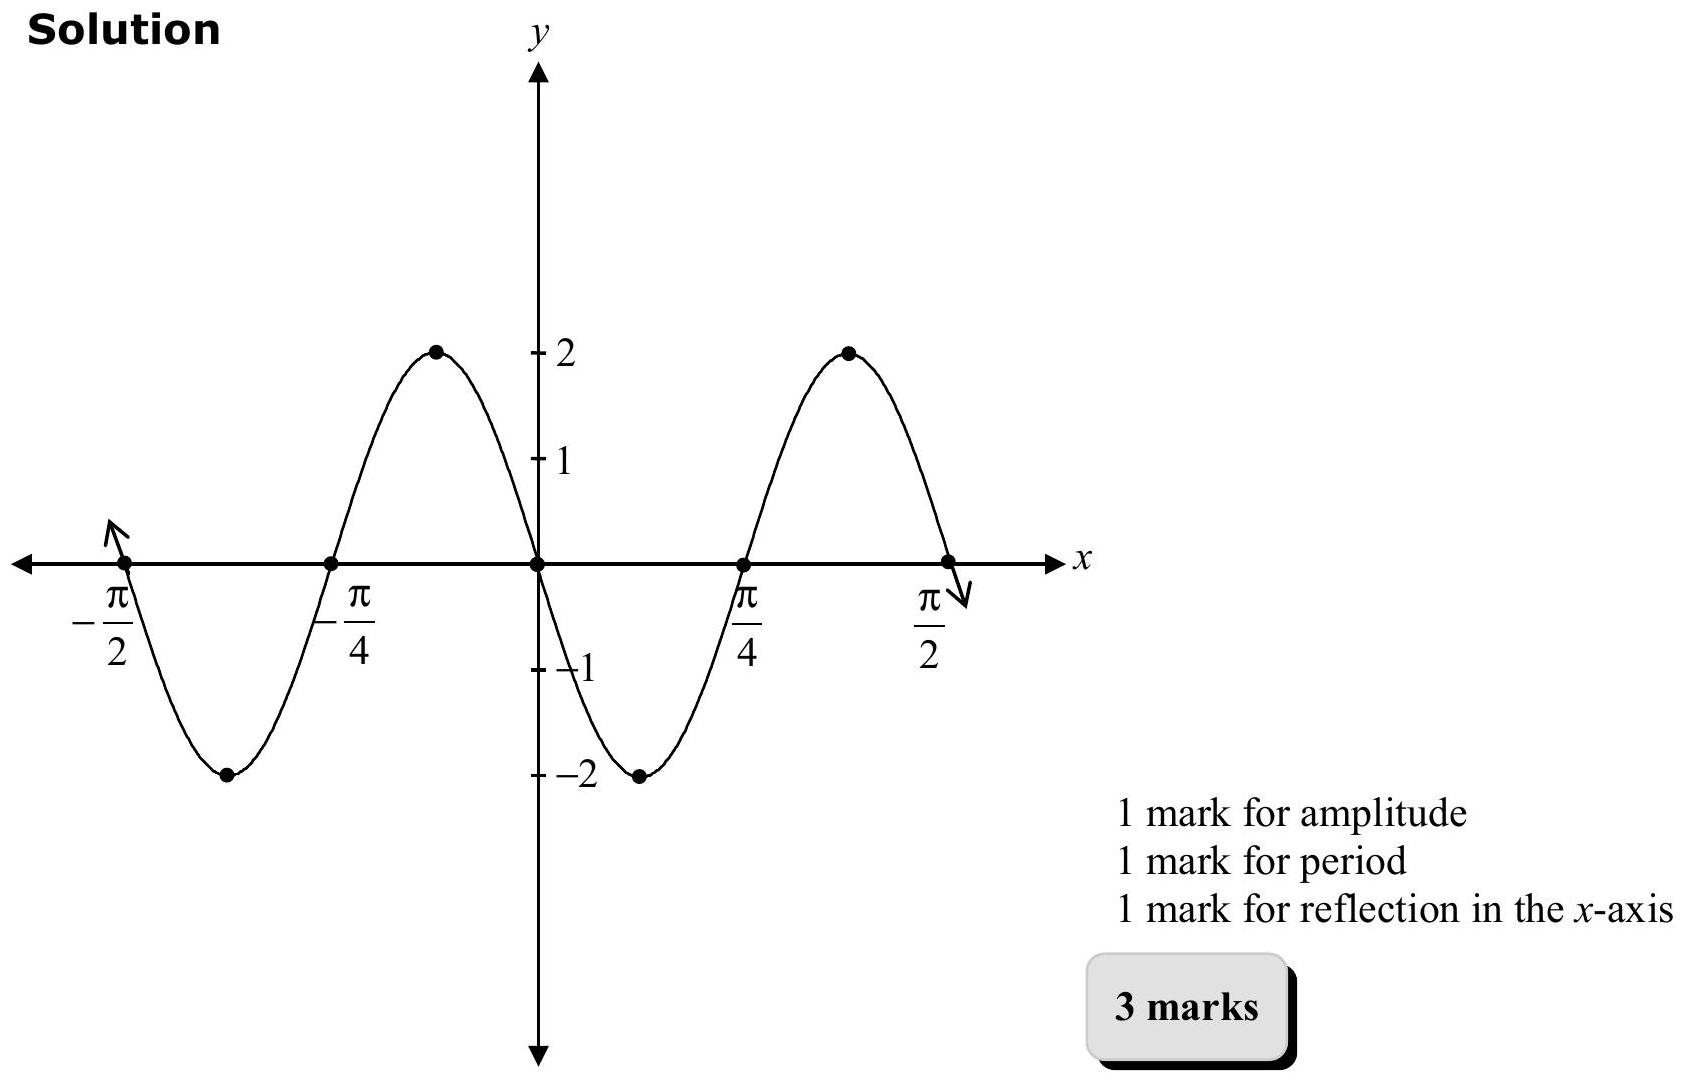
\includegraphics[max width=\textwidth, alt={}, center]{f67fedaf-ea11-42ad-a16e-f30d2fcf2bd3-109_1075_1683_487_150}

Evaluate:

$$
\frac{1}{2} \log _{3} 144-\log _{3} 4+2 \log _{3} 3
$$

\section*{Solution}
$\log _{3}(144)^{\frac{1}{2}}-\log _{3} 4+\log _{3}(3)^{2} \quad 1$ mark for power rule\\
$\log _{3} 12-\log _{3} 4+\log _{3} 9$\\
$\log _{3}\left(\frac{12 \cdot 9}{4}\right)$\\
$\log _{3} 27$\\
3\\
$\frac{1}{2}$ mark for product rule\\
$\frac{1}{2}$ mark for quotient rule

1 mark for evaluating a logarithm\\
3 marks

Match each function with its correct description.\\
a) The graph of this function has a vertical asymptote at $x=-1$.\\
b) The graph of this function has a point of discontinuity (hole) at $x=3$.\\
c) The graph of this function has a horizontal asymptote at $y=4$.\\
d) The domain of this function is $x \in \mathbb{R}$.

Place the appropriate letter in this column.

\section*{Solution}
$f(x)=\frac{4}{x^{2}+1}$\\
d)\\
$g(x)=\frac{4 x}{x+3}$\\
c)\\
$h(x)=\frac{4(x-3)(x+2)}{(x-3)}$\\
b)\\
$k(x)=\frac{4(x-3)}{(x+3)(x+1)}$ $\_\_\_\_$\\
a)\\
$\frac{1}{2}$ mark for each correct answer

The point ( $-3,4$ ) is on the graph of $y=\frac{1}{2} f(3 x)$.\\
State the coordinates of the corresponding point on the graph of $y=f(x)$.

\section*{Solution}
$(-9,8)$\\
$\frac{1}{2}$ mark for each coordinate\\
1 mark

Sketch the graph of $y=-2(x-1)(x-3)(x+1)$.

\section*{Solution}
\begin{center}
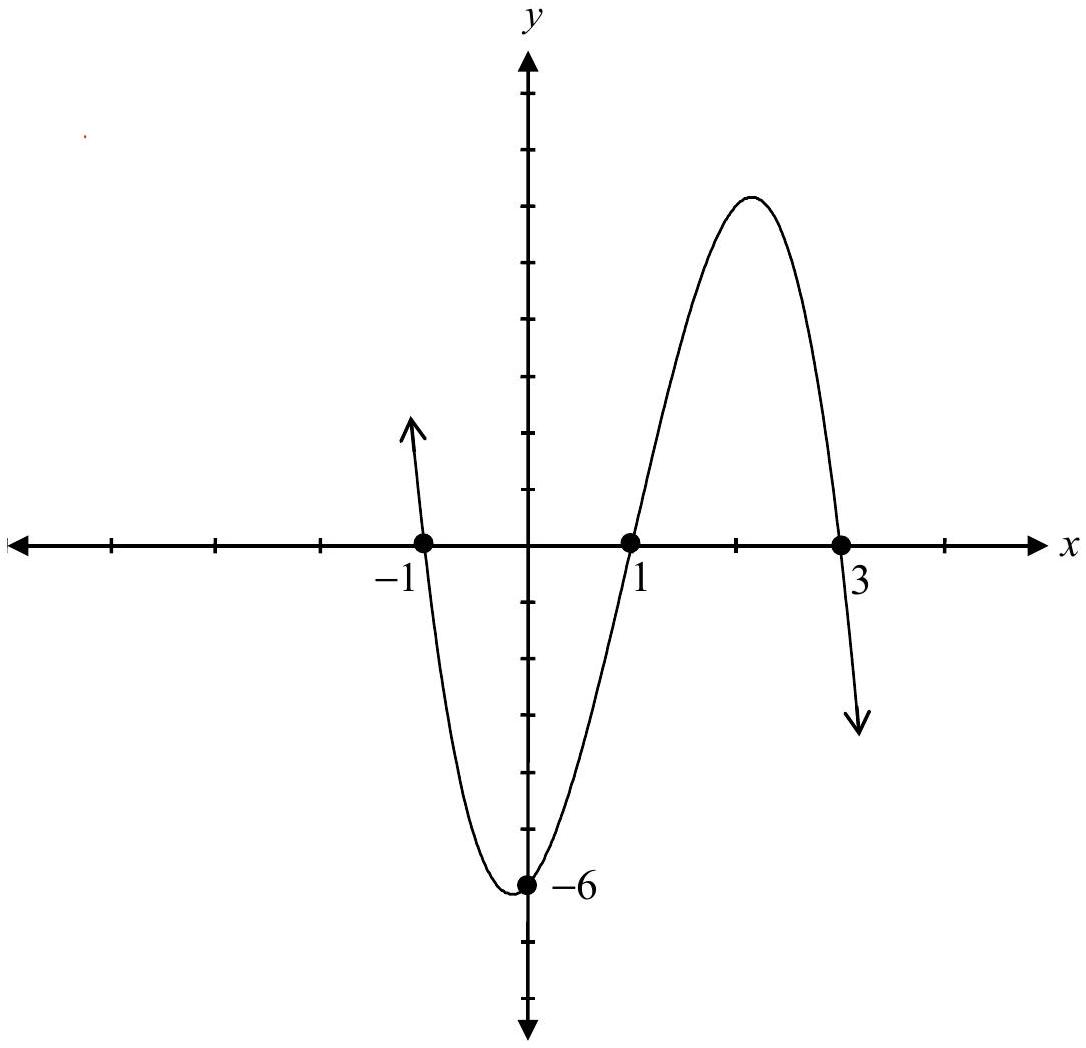
\includegraphics[max width=\textwidth, alt={}]{f67fedaf-ea11-42ad-a16e-f30d2fcf2bd3-113_1048_1086_575_167}
\end{center}

1 mark for $x$-intercepts 1 mark for $y$-intercept 1 mark for end behaviour 3 marks\\
a) Verify that the equation $\frac{1-\sin ^{2} x}{\cos x}=\frac{\sin 2 x}{2 \sin x}$ is true for $x=\frac{\pi}{3}$.\\
b) Explain why verifying the equation for $x=\frac{\pi}{3}$ is insufficient to conclude that the equation is an identity.

\section*{Solution}
a) \begin{tabular}{rl}
$\frac{1-\sin ^{2}\left(\frac{\pi}{3}\right)}{\cos \frac{\pi}{3}}$ & $\frac{\sin 2\left(\frac{\pi}{3}\right)}{2 \sin \frac{\pi}{3}}$ \\
 & $\frac{1-\left(\frac{\sqrt{3}}{2}\right)^{2}}{\frac{1}{2}}$ \\
$\frac{\frac{\frac{\sqrt{3}}{2}}{2\left(\frac{\sqrt{3}}{2}\right)}}{}$ &  \\
$\frac{1-\frac{3}{4}}{\frac{1}{2}}$ & 1 mark for exact values $\left(1 / 2\right.$ mark for $\sin \frac{\pi}{3}, 1 / 2$ mark for $\left.\cos \frac{\pi}{3}\right)$ \\
$\frac{\frac{\sqrt{3}}{2}}{\frac{1}{3}}$ & 1 mark for simplification $(1 / 2$ mark for LHS, $1 / 2$ mark for RHS $)$ \\
$\frac{\frac{1}{2}}{2}$ & \multicolumn{1}{|l}{$\frac{1}{2}$} \\
$\frac{1}{2}$ & \multicolumn{1}{c}{LHS = RHS} \\
\end{tabular}

b) Proving that it is true for one value does not mean that it is true for all values.

Evaluate:

$$
\frac{{ }_{7} P_{2}}{{ }_{7} P_{5}}
$$

\section*{Solution}
\begin{center}
\begin{tabular}{|l|l|}
\hline
$\frac{\frac{7!}{(7-2)!}}{\frac{7!}{(7-5)!}}$ & $\frac{1}{2}$ mark for substitution \\
\hline
$\frac{7!}{\frac{5!}{7!}}$ &  \\
\hline
$\frac{2!}{5!}$ & $\frac{1}{2}$ mark for simplification \\
\hline
$\frac{2 \times 1}{5 \times 4 \times 3 \times 2 \times 1} \frac{1}{60}$ & 2 marks \\
\hline
\end{tabular}
\end{center}

Use the graph of $y=f(x)$ to sketch the graph of $y=f(3 x)+1$.\\
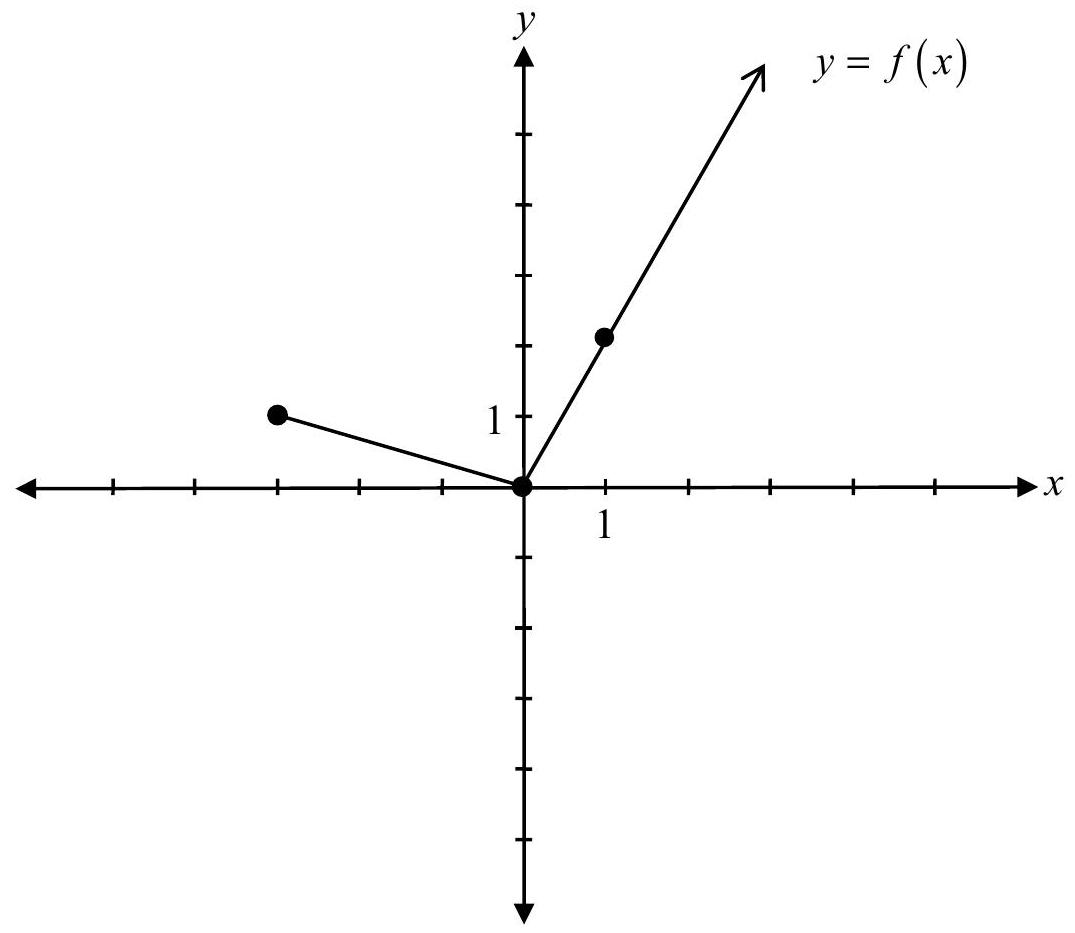
\includegraphics[max width=\textwidth, alt={}, center]{f67fedaf-ea11-42ad-a16e-f30d2fcf2bd3-116_933_1075_483_382}

\section*{Solution}
\begin{center}
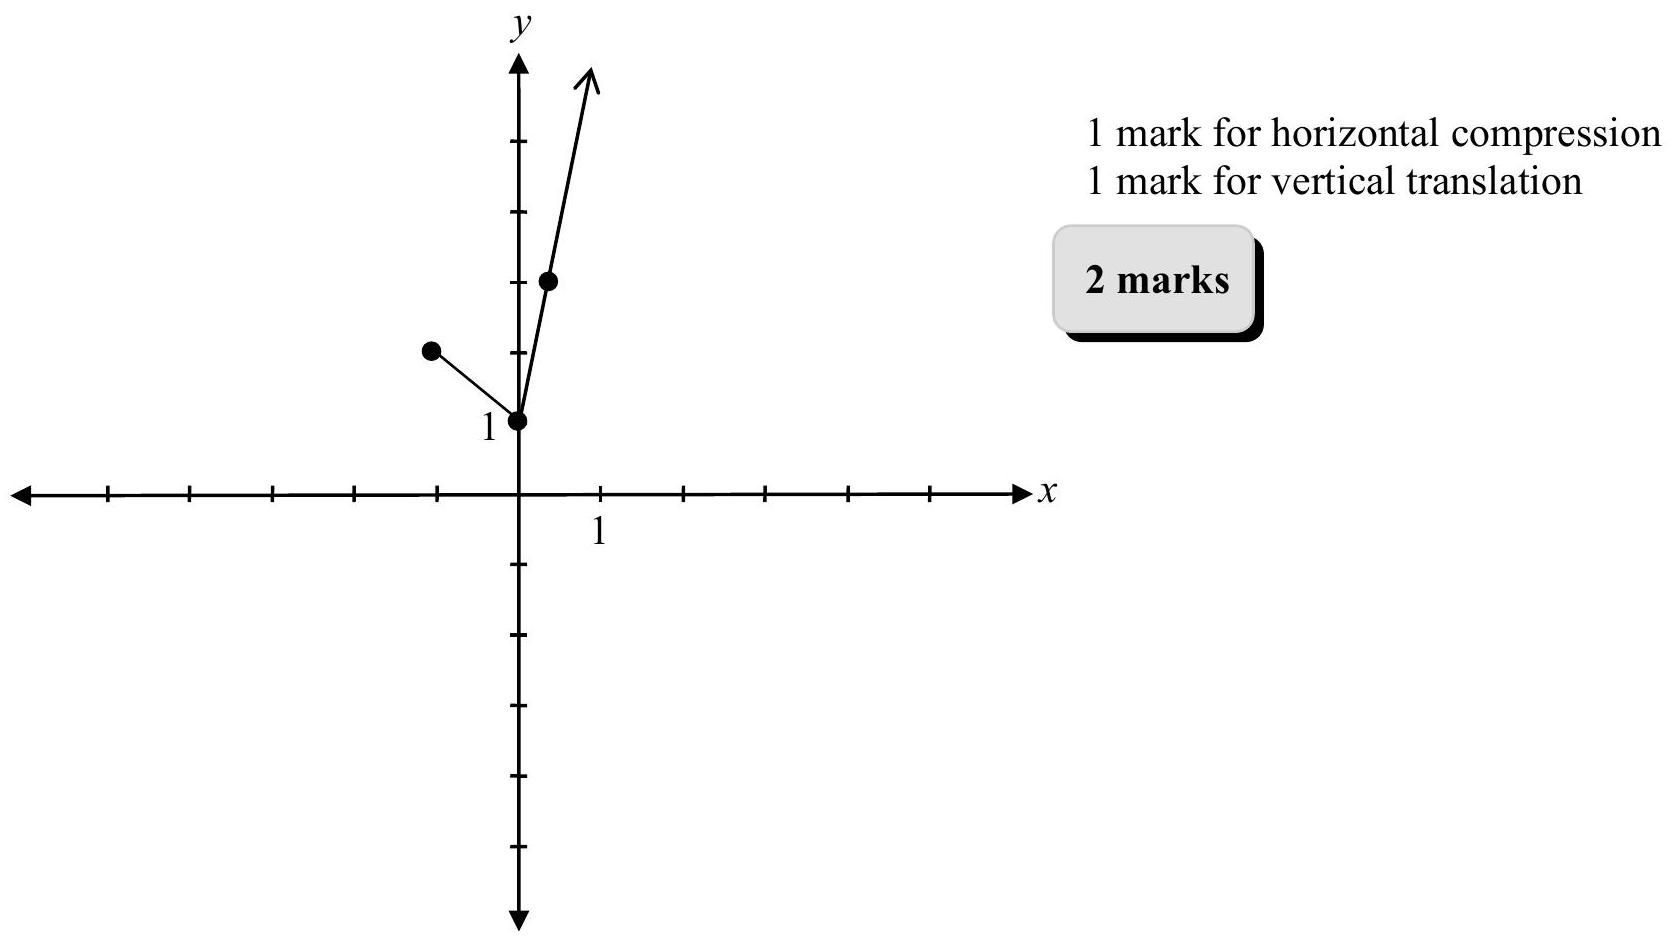
\includegraphics[max width=\textwidth, alt={}]{f67fedaf-ea11-42ad-a16e-f30d2fcf2bd3-116_942_1673_1572_171}
\end{center}

Solve the following equation:

$$
\log _{4}(x+2)+\log _{4} 3=\log _{4} x
$$

\section*{Solution}
\section*{Method 1}
$$
\begin{aligned}
\log _{4}(x+2)+\log _{4} 3 & =\log _{4} x \\
\log _{4}[(x+2) 3] & =\log _{4} x \\
3(x+2) & =x \\
3 x+6 & =x \\
x & =-3
\end{aligned}
$$

No solution

\section*{Method 2}
$$
\begin{aligned}
\log _{4}(x+2)+\log _{4} 3 & =\log _{4} x \\
\log _{4}(x+2)+\log _{4} 3-\log _{4} x & =0 \\
\log _{4}\left[\frac{3(x+2)}{x}\right] & =0 \\
4^{0} & =\frac{3 x+6}{x} \\
x & =-3 \\
x & <-3
\end{aligned}
$$

1 mark for product rule\\
1 mark for equating arguments\\
$\frac{1}{2}$ mark for solving for $x$\\
$\frac{1}{2}$ mark for rejecting extraneous root

\section*{3 marks}
1 mark for logarithmic rules ( $\frac{1}{2}$ mark for product rule; $\frac{1}{2}$ mark for quotient rule)\\
1 mark for exponential form\\
$\frac{1}{2}$ mark for solving for $x$\\
$\frac{1}{2}$ mark for rejecting extraneous root\\
3 marks

Determine the coordinates of the point of discontinuity (hole) for the graph of the function $y=\frac{(2-x)(x-3)}{(x-2)}$.

\section*{Solution}
$$
\begin{aligned}
& x \neq 2 \\
& y=-(x-3) \\
& y=-(2-3) \\
& y=1 \\
& \quad(2,1)
\end{aligned}
$$

1 mark for point of discontinuity (hole) at $(2,1)$\\
( $\frac{1}{2}$ mark for $x=2, \frac{1}{2}$ mark for consistent $y$-coordinate)\\
1 mark

Evaluate and simplify $\sec \left(\frac{5 \pi}{6}\right) \cdot \tan \left(-\frac{\pi}{6}\right)$.

\section*{Solution}
$\left(-\frac{2}{\sqrt{3}}\right) \cdot\left(-\frac{1}{\sqrt{3}}\right)$\\
1 mark for $\sec \left(\frac{5 \pi}{6}\right)\left(\frac{1}{2}\right.$ mark for value, $1 / 2$ mark for quadrant)\\
$\frac{2}{3}$\\
1 mark for $\tan \left(-\frac{\pi}{6}\right)\left(\frac{1}{2}\right.$ mark for value, $1 / 2$ mark for quadrant)\\
2 marks

Sketch the graph of the following function:

$$
y=-2 \sqrt{x-3}
$$

\section*{Solution}
\section*{Method 1}
\begin{center}
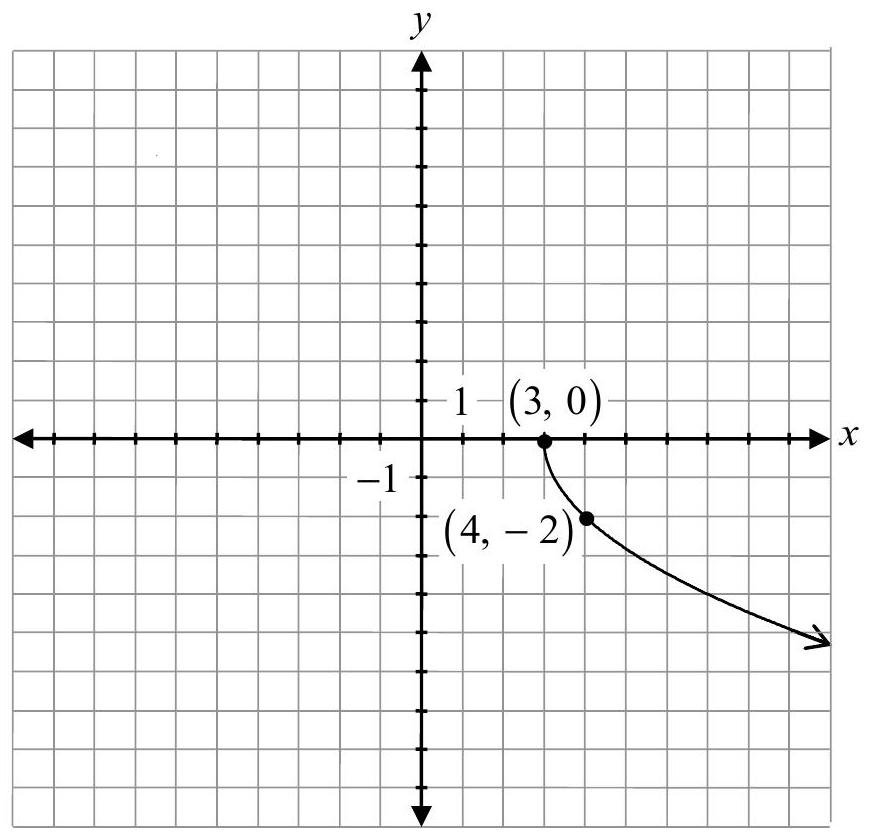
\includegraphics[max width=\textwidth, alt={}]{f67fedaf-ea11-42ad-a16e-f30d2fcf2bd3-120_837_869_700_236}
\end{center}

1 mark for shape (graph of a radical function)\\
1 mark for vertical reflection\\
1 mark for horizontal shift\\
1 mark for vertical stretch\\
4 marks

\section*{Method 2}
\begin{center}
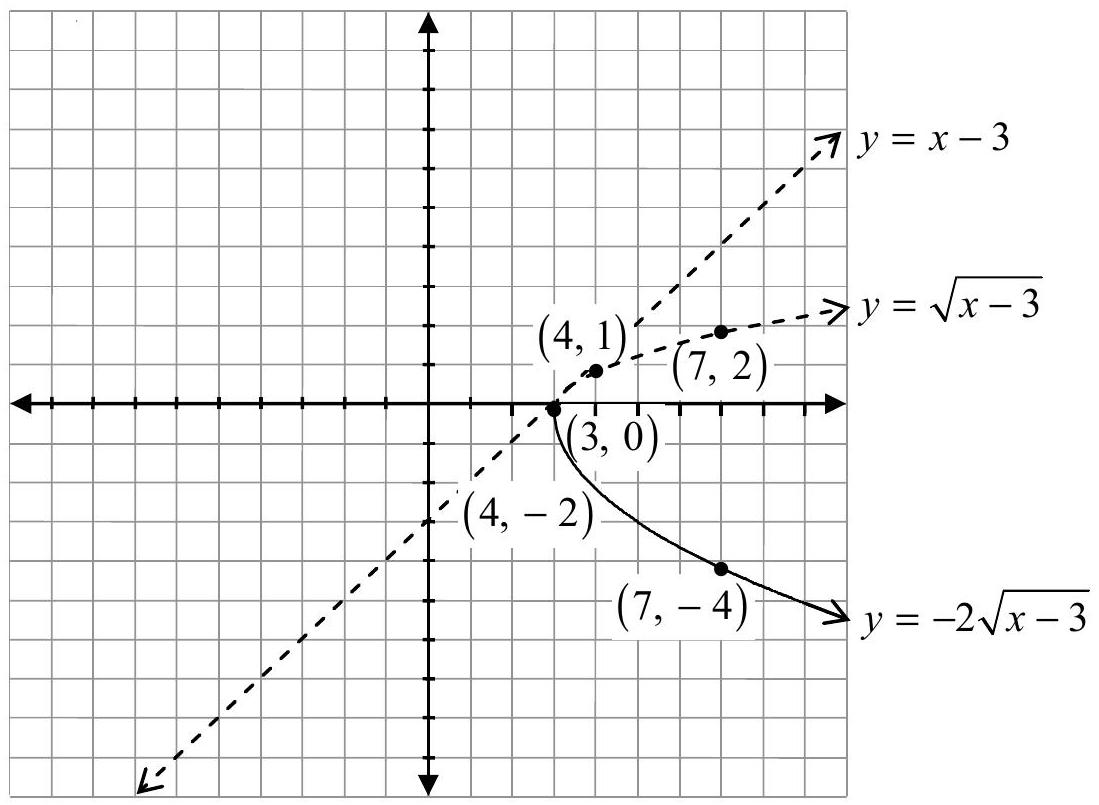
\includegraphics[max width=\textwidth, alt={}]{f67fedaf-ea11-42ad-a16e-f30d2fcf2bd3-120_805_1099_1677_180}
\end{center}

1 mark for invariant points where $y=0$ and $y=1$ ( $\frac{1}{2}$ mark for each point)\\
1 mark for domain of $[3, \infty)$\\
$\frac{1}{2}$ mark for shape between invariant points\\
$\frac{1}{2}$ mark for shape to the right of the invariant points\\
1 mark for applying transformations (vertical stretch, vertical reflection)

\section*{4 marks}
Sketch the graph of $f(x)=\frac{2 x+3}{x+2}$.

\section*{Solution}
\begin{center}
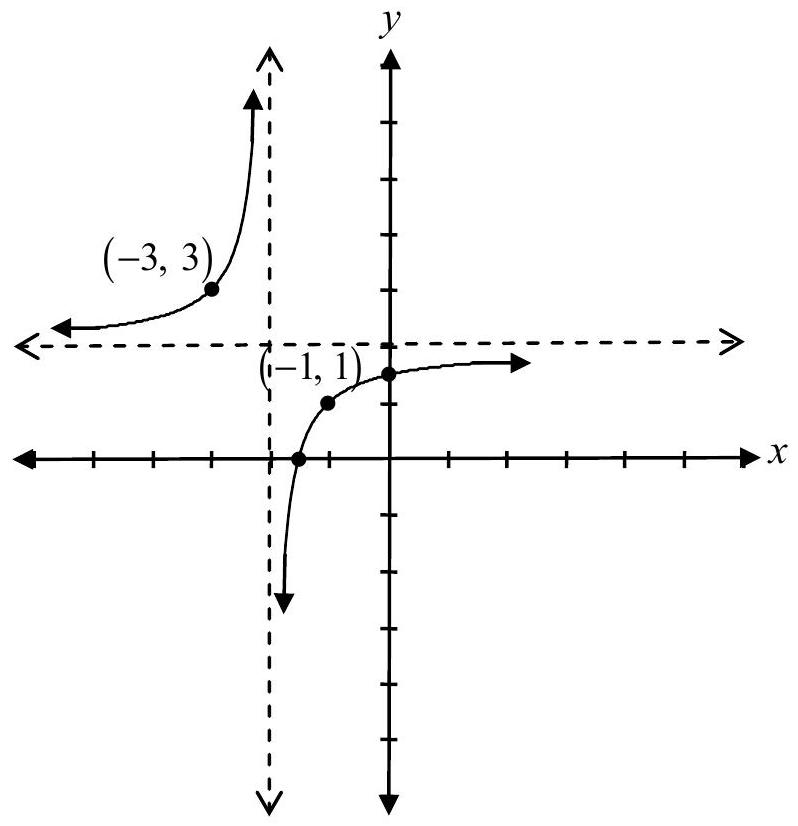
\includegraphics[max width=\textwidth, alt={}]{f67fedaf-ea11-42ad-a16e-f30d2fcf2bd3-121_826_798_625_283}
\end{center}

1 mark for vertical asymptote\\
1 mark for horizontal asymptote\\
$\frac{1}{2}$ mark for graph left of the vertical asymptote $\frac{1}{2}$ mark for graph right of the vertical asymptote

3 marks\\
a) Given the functions $f(x)=\sqrt{4+x}$ and $g(x)=|3 x-6|$, evaluate $f(g(-5))$.\\
b) Is it possible to evaluate $g(f(-5))$ ?

Justify your answer.

\section*{Solution}
a) $g(-5)=|3(-5)-6|$\\
$g(-5)=21$\\
1 mark for $g(-5)$\\
$f(21)=\sqrt{4+21}$\\
$=\sqrt{25}$\\
$=5$\\
1 mark for consistent value of $f(g(-5))$

\section*{2 marks}
b) No, because $f(x)$ is undefined when $x=-5$

1 mark for justification\\
or

$$
\begin{aligned}
& f(-5)=\sqrt{4+(-5)} \\
& f(-5)=\sqrt{-1}
\end{aligned}
$$

$f(-5)$ is undefined because you cannot evaluate the square root of a negative number.

Identify which of these values is greater. Justify your answer.

$$
\log _{5} 80 \text { or } \log _{3} 30
$$

\section*{Solution}
$5^{2}=25$\\
$5^{3}=125$ $\log _{5} 80$ is less than 3\\
$3^{3}=27$\\
$3^{4}=81 \quad \log _{3} 30$ is more than 3\\
$\therefore \log _{3} 30$ is greater\\
1 mark for justification\\
1 mark

Given $\cos \alpha=\frac{3}{5}$, where $\alpha$ is in quadrant IV, and $\cos \beta=-\frac{2}{3}$, where $\beta$ is in quadrant II, determine the exact value of $\sin (\alpha-\beta)$.

\section*{Solution}
\begin{center}
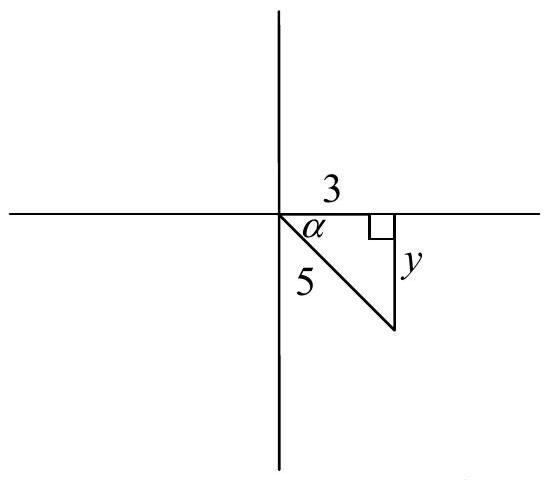
\includegraphics[max width=\textwidth, alt={}]{f67fedaf-ea11-42ad-a16e-f30d2fcf2bd3-124_480_551_711_232}
\end{center}

$$
\begin{aligned}
x^{2}+y^{2} & =r^{2} \\
9+y^{2} & =25 \\
y^{2} & =16 \\
y & = \pm 4 \\
y & =-4
\end{aligned}
$$

$\frac{1}{2}$ mark for value of $y$

$$
\sin \alpha=-\frac{4}{5}
$$

\begin{center}
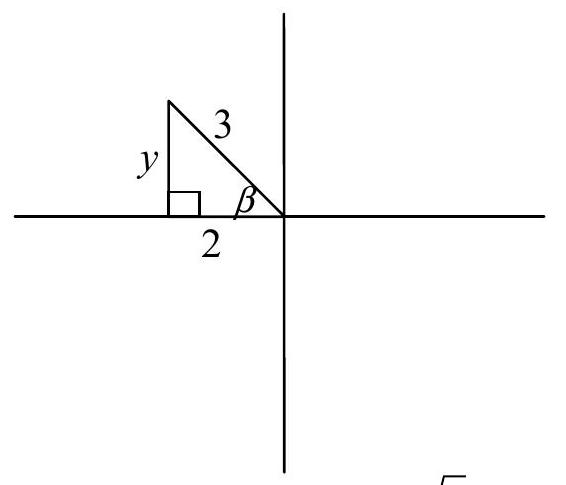
\includegraphics[max width=\textwidth, alt={}]{f67fedaf-ea11-42ad-a16e-f30d2fcf2bd3-124_485_566_1297_227}
\end{center}

$$
\begin{aligned}
x^{2}+y^{2} & =r^{2} \\
4+y^{2} & =9 \\
y^{2} & =5 \\
y & =\sqrt[ \pm]{5} \\
y & =\sqrt{5} \quad 1 / 2 \text { mark for value of } y
\end{aligned}
$$

$$
\sin \beta=\frac{\sqrt{5}}{3}
$$

$$
\begin{aligned}
\sin (\alpha-\beta) & =\sin \alpha \cos \beta-\cos \alpha \sin \beta \\
& =\left(-\frac{4}{5}\right)\left(-\frac{2}{3}\right)-\left(\frac{3}{5}\right)\left(\frac{\sqrt{5}}{3}\right) \\
& =\frac{8-3 \sqrt{5}}{15}
\end{aligned}
$$

$\frac{1}{2}$ mark for $\sin \alpha$\\
$\frac{1}{2}$ mark for $\sin \beta$\\
1 mark for substitution into correct identity

Determine the number of possible sandwiches from the following menu.

\section*{MENU}
Select one item from each column:

\begin{center}
\begin{tabular}{cccc}
$\underline{\text { Bread }}$ & $\underline{\text { Sauce }}$ & $\underline{\text { Meat }}$ & Vegetable \\
\begin{tabular}{c}
White \\
Rye \\
Brown \\
\end{tabular} & \begin{tabular}{c}
Mayo \\
Mustard \\
\end{tabular} & \begin{tabular}{c}
Turkey \\
Ham \\
Roast Beef \\
Chicken \\
\end{tabular} & \begin{tabular}{c}
Tomato \\
Onion \\
Lettuce \\
\end{tabular} \\
\end{tabular}
\end{center}

\section*{Solution}
$3 \times 2 \times 4 \times 3$\\
72 sandwiches

A pizza with a diameter of 15 inches is cut into equal slices, each with a central angle of $36^{\circ}$. Determine the length of the crust on the outer edge of one slice of pizza.

\section*{Solution}
$\frac{36^{\circ}}{180^{\circ}}=\frac{\theta}{\pi}$

$$
\theta=\frac{\pi}{5}
$$

1 mark for conversion

$$
\begin{aligned}
& s=\theta r \\
& s=\left(\frac{\pi}{5}\right)\left(\frac{15}{2}\right) \\
& s=\frac{3 \pi}{2} \text { inches }
\end{aligned}
$$

1 mark for substitution

\section*{2 marks}
or\\
$s=4.712$ inches

There are 9 girls and 7 boys in a math class from which a committee of 5 is to be chosen.\\
a) How many different committees of 5 can be formed if one of the boys, William, must be on the committee?\\
b) How many different committees of 5 can be formed if there must be 2 girls and 3 boys on the committee?

\section*{Solution}
a) ${ }_{1} C_{1} \cdot{ }_{15} C_{4}=1365$\\
b) ${ }_{9} C_{2} \cdot{ }_{7} C_{3}=1260$\\
$\frac{1}{2}$ mark for ${ }_{9} C_{2}$\\
$\frac{1}{2}$ mark for ${ }_{7} C_{3}$\\
1 mark for the product of combinations\\
2 marks

Note(s):

\begin{itemize}
  \item ${ }_{1} C_{1}$ does not need to be shown
\end{itemize}

Solve the following equation over the interval $[0,2 \pi]$ :

$$
\sin ^{2} \theta+6 \sin \theta-2=0
$$

\section*{Solution}
$$
\begin{aligned}
\sin \theta & =\frac{-6 \pm \sqrt{(6)^{2}-4(1)(-2)}}{2(1)} & & \\
\sin \theta & =\frac{-6 \pm \sqrt{36+8}}{2} & & \\
\sin \theta & =\frac{-6 \pm \sqrt{44}}{2} & & \\
\sin \theta & =0.316624 \ldots & \sin \theta=-6.316624 \ldots & \\
\theta_{r} & =0.322169 & & \\
\theta & =0.322 & \text { no solution } & \\
\theta & & & \begin{array}{l}
2 \text { marks for solving for } \theta(1 / 2 \text { mark for each } \\
\text { value, } 1 \text { mark for indicating no solution })
\end{array} \\
\theta & & & \mathbf{3} \text { marks }
\end{aligned}
$$

Solve:

$$
6(5)^{3 x+2}=9^{2-x}
$$

\section*{Solution}
$$
\begin{aligned}
\log \left[6(5)^{3 x+2}\right] & =\log 9^{2-x} \\
\log 6+\log 5^{3 x+2} & =\log 9^{2-x}
\end{aligned}
$$

$$
\begin{aligned}
\log 6+(3 x+2) \log 5 & =(2-x) \log 9 \\
\log 6+3 x \log 5+2 \log 5 & =2 \log 9-x \log 9 \\
3 x \log 5+x \log 9 & =2 \log 9-2 \log 5-\log 6 \\
x(3 \log 5+\log 9) & =2 \log 9-2 \log 5-\log 6 \\
x & =\frac{2 \log 9-2 \log 5-\log 6}{3 \log 5+\log 9} \\
x & =-0.087707 \\
& =-0.088
\end{aligned}
$$

$\frac{1}{2}$ mark for applying logarithms\\
1 mark for product law

1 mark for power law\\
$\frac{1}{2}$ mark for collecting terms with $x$\\
$\frac{1}{2}$ mark for solving for $x$\\
$\frac{1}{2}$ mark for evaluating quotient of logarithms

Solve $(2 \sin \theta-1)(\sin \theta+1)=0$ where $\theta \in \mathbb{R}$.

\section*{Solution}
$$
\begin{aligned}
2 \sin \theta-1 & =0 \\
\sin \theta & =\frac{1}{2} \\
\theta_{r} & =\frac{\pi}{6} \\
\theta & =\frac{\pi}{6}+2 k \pi, k \in \mathbb{Z} \\
\theta & =\frac{5 \pi}{6}+2 k \pi, k \in \mathbb{Z}
\end{aligned}
$$

$$
\begin{aligned}
\sin \theta+1 & =0 \\
\sin \theta & =-1
\end{aligned}
$$

1 mark for solving for $\sin \theta$

2 marks for solving for $\theta$ ( 1 mark for each branch)\\
1 mark for general solution\\
or

$$
\begin{aligned}
\theta_{r} & =30^{\circ} \\
\theta & =30^{\circ}+360^{\circ} k, k \in \mathbb{Z} \\
\theta & =150^{\circ}+360^{\circ} k, k \in \mathbb{Z}
\end{aligned}
$$

$$
\begin{aligned}
\theta_{r} & =\frac{3 \pi}{2} \\
\theta & =\frac{3 \pi}{2}+2 k \pi, \quad k \in \mathbb{Z}
\end{aligned}
$$

or

$$
\begin{aligned}
\theta_{r} & =270^{\circ} \\
\theta & =270^{\circ}+360^{\circ} k, k \in \mathbb{Z}
\end{aligned}
$$

The roots of the polynomial equation $3(x-2)(x+1)^{2}=0$ are $x=2$ and $x=-1$.\\
Explain what these roots represent on the graph of $p(x)=3(x-2)(x+1)^{2}$.

\section*{Solution}
They are the $x$-intercepts of the graph of $p(x)$.

Determine an equation for $g(x)$ as a transformation of $f(x)$.\\
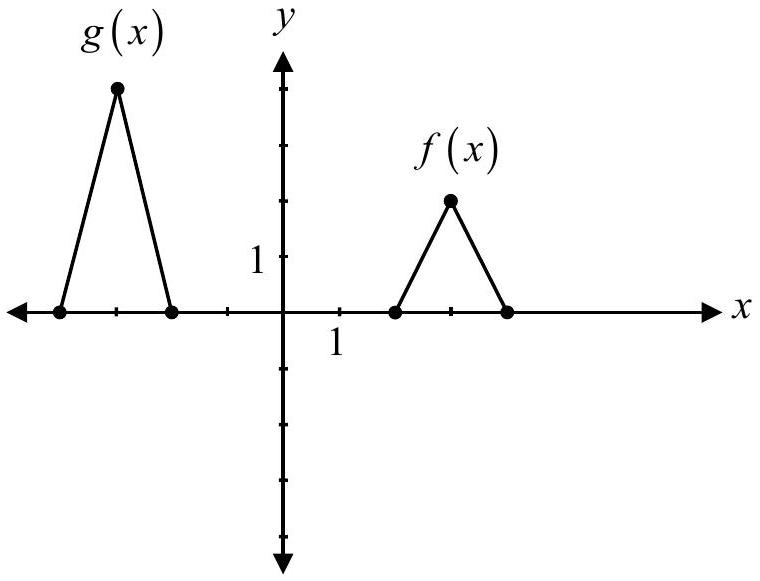
\includegraphics[max width=\textwidth, alt={}, center]{f67fedaf-ea11-42ad-a16e-f30d2fcf2bd3-132_581_760_464_298}

\section*{Solution}
$g(x)=\underline{2 f(x+6)}$\\
1 mark for vertical stretch\\
1 mark for horizontal translation\\
2 marks\\
or

1 mark for vertical stretch\\
$g(x)=2 f(-x)$\\
1 mark for horizontal reflection

2 marks

A student must determine the factors of $5 x^{4}-2 x^{3}+4 x-1$. He used $5,-2,4$, and -1 as the coefficients of the polynomial when using synthetic division.\\
Explain the student's error.

\section*{Solution}
The student did not write the coefficient of 0 for the $x^{2}$ term.

Describe the transformations of $y=f(x)$ when asked to sketch the graph of $y=-f(x-4)$.

\section*{Solution}
$f(x)$ is reflected over the $x$-axis and translated 4 units to the right.\\
1 mark for vertical reflection\\
1 mark for horizontal translation\\
2 marks

Prove the identity below for all permissible values of $\theta$ :

$$
\sin \theta+\frac{\cos \theta}{\tan \theta}=\frac{1}{\cos \theta \tan \theta}
$$

\section*{Solution}
\section*{Method 1}
\begin{center}
\begin{tabular}{|l|l|}
\hline
Left-Hand Side & Right-Hand Side \\
\hline
$\sin \theta+\frac{\cos \theta}{\tan \theta}$ & $\frac{1}{\cos \theta \tan \theta}$ \\
\hline
$\sin \theta+\frac{\cos \theta}{\frac{\sin \theta}{\cos \theta}}$ & $\frac{1}{\cos \theta \frac{\sin \theta}{\cos \theta}}$ \\
\hline
$\sin \theta+\frac{\cos ^{2} \theta}{\sin \theta}$ & $\frac{1}{\sin \theta}$ \\
\hline
$\frac{\sin ^{2} \theta+\cos ^{2} \theta}{\sin \theta}$ &  \\
\hline
$\frac{1}{\sin \theta}$ &  \\
\hline
\end{tabular}
\end{center}

1 mark for correct substitution of identities

1 mark for algebraic strategies

1 mark for logical process to prove an identity 3 marks

\section*{Method 2}
\begin{center}
\begin{tabular}{|l|l|}
\hline
Left-Hand Side & Right-Hand Side \\
\hline
\multirow[t]{9}{*}{$\sin \theta+\frac{\cos \theta}{\tan \theta}$} & $\frac{1}{\cos \theta \tan \theta}$ \\
\hline
 &  \\
\hline
 & $\frac{1}{\cos \theta \frac{\sin \theta}{\cos \theta}}$ \\
\hline
 & $\frac{1}{\sin \theta}$ \\
\hline
 & $\frac{\sin ^{2} \theta+\cos ^{2} \theta}{\sin \theta}$ \\
\hline
 & $\frac{\sin ^{2} \theta}{\sin \theta}+\frac{\cos ^{2} \theta}{\sin \theta}$ \\
\hline
 & $\sin \theta+\cos \theta \frac{\cos \theta}{\sin \theta}$ \\
\hline
 & $\sin \theta+\cos \theta \cot \theta$ \\
\hline
 & $\sin \theta+\frac{\cos \theta}{\tan \theta}$ \\
\hline
\end{tabular}
\end{center}

1 mark for correct substitution of identities

1 mark for algebraic strategies

1 mark for logical process to prove an identity

Describe how to use the graphs of $f(x)=3 \sin x$ and $g(x)=2$ to solve the equation $3 \sin x=2$.\\
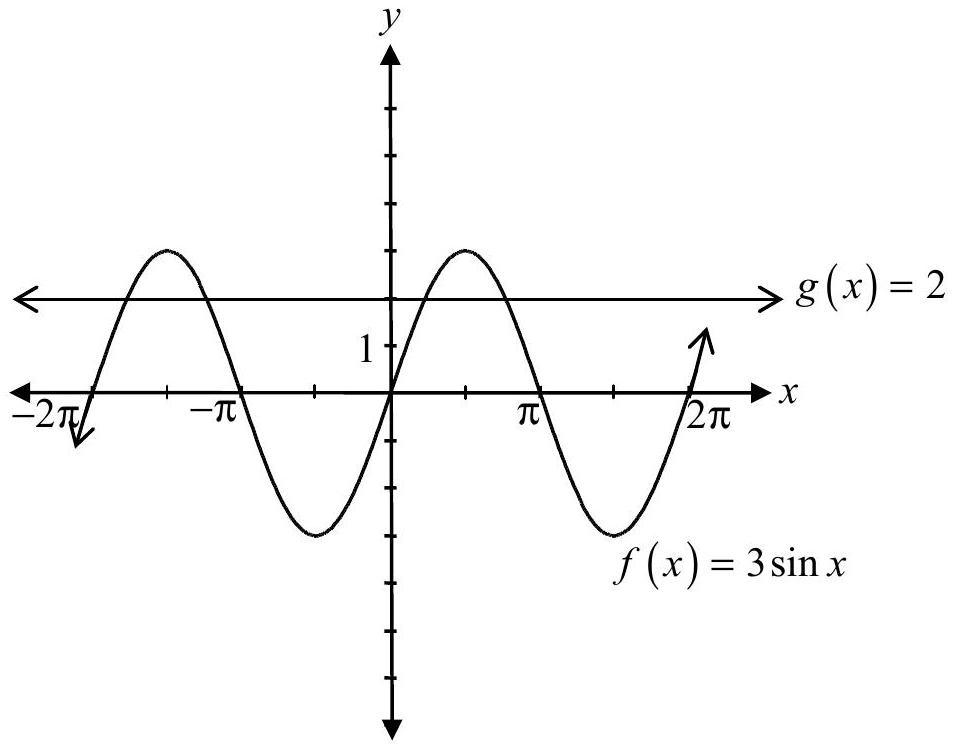
\includegraphics[max width=\textwidth, alt={}, center]{f67fedaf-ea11-42ad-a16e-f30d2fcf2bd3-137_748_955_537_212}

\section*{Solution}
The solution will be the $x$-values where the two graphs intersect.

A hockey arena has 5 doors.\\
Determine the number of ways that you can enter through one door but exit through a different door.

\section*{Solution}
5 • $4=20$ ways\\
1 mark

Given that $(x+3)$ is one of the factors, express $2 x^{3}+7 x^{2}+2 x-3$ as a product of factors.

\section*{Solution}
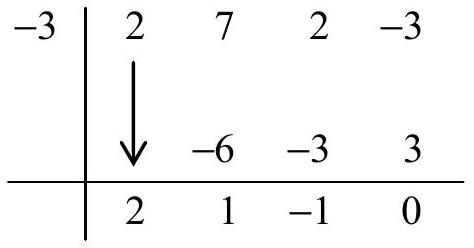
\includegraphics[max width=\textwidth, alt={}, center]{f67fedaf-ea11-42ad-a16e-f30d2fcf2bd3-139_248_474_601_171}\\
$\frac{1}{2}$ mark for $x=-3$\\
1 mark for synthetic division (or for any other equivalent strategy)

$$
(x+3)\left(2 x^{2}+x-1\right)
$$

$\frac{1}{2}$ mark for consistent product of factors\\
or\\
2 marks\\
$(x+3)(2 x-1)(x+1)$

Identify the maximum number of $x$-intercepts for a polynomial function of degree 3 .\\
a) 1\\
b) 2\\
c) 3\\
d) 4

Question 15

The graph of $y=f(x)$ contains the point $(a, b)$. The graph of $g(x)$ is a transformation of the graph of $f(x)$ and contains the point $(3 a, b)$.

Identify the function that represents $g(x)$.\\
a) $g(x)=f(3 x)$\\
b) $g(x)=3 f(x)$\\
c) $g(x)=f\left(\frac{x}{3}\right)$\\
d) $g(x)=\frac{1}{3} f(x)$

Question 16

The angle 2.95 radians, in standard position, terminates in quadrant:\\
a) I\\
b) II\\
c) III\\
d) IV

Evaluate:

$$
2 \sin \frac{\pi}{8} \cos \frac{\pi}{8}
$$

a) $\frac{1}{2}$\\
b) $\frac{\sqrt{2}}{2}$\\
c) 1\\
d) $\sqrt{2}$

\section*{Question 18}
Identify which of the following represents the 5th term in the expansion of $\left(4 x^{2}-2 y^{3}\right)^{15}$.\\
a) ${ }_{15} C_{5}\left(4 x^{2}\right)^{10}\left(-2 y^{3}\right)^{5}$\\
b) ${ }_{15} C_{5}\left(4 x^{2}\right)^{11}\left(-2 y^{3}\right)^{4}$\\
c) ${ }_{15} C_{4}\left(4 x^{2}\right)^{10}\left(-2 y^{3}\right)^{5}$\\
d) ${ }_{15} C_{4}\left(4 x^{2}\right)^{11}\left(-2 y^{3}\right)^{4}$

Identify which of the following graphs of polynomial functions has a zero with a multiplicity of 3 .\\
a)\\
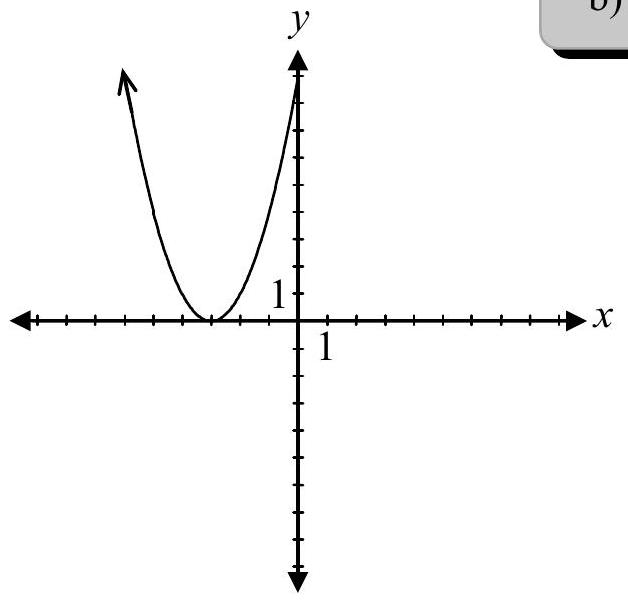
\includegraphics[max width=\textwidth, alt={}, center]{f67fedaf-ea11-42ad-a16e-f30d2fcf2bd3-142_604_628_494_399}\\
b)\\
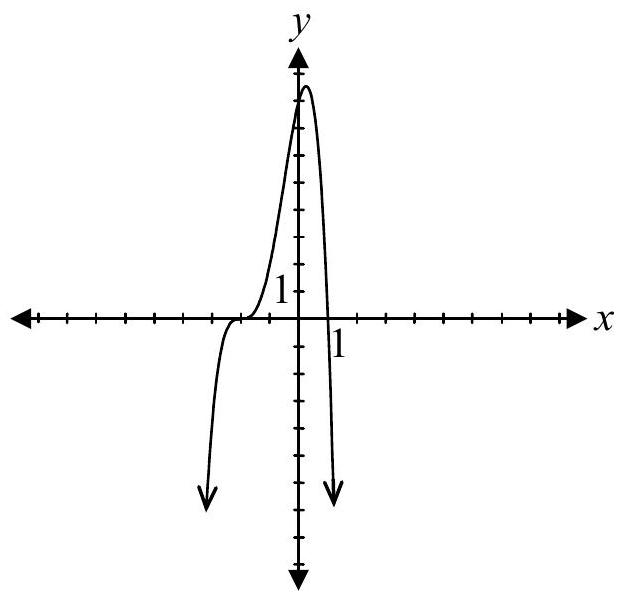
\includegraphics[max width=\textwidth, alt={}, center]{f67fedaf-ea11-42ad-a16e-f30d2fcf2bd3-142_601_621_489_1130}\\
c)\\
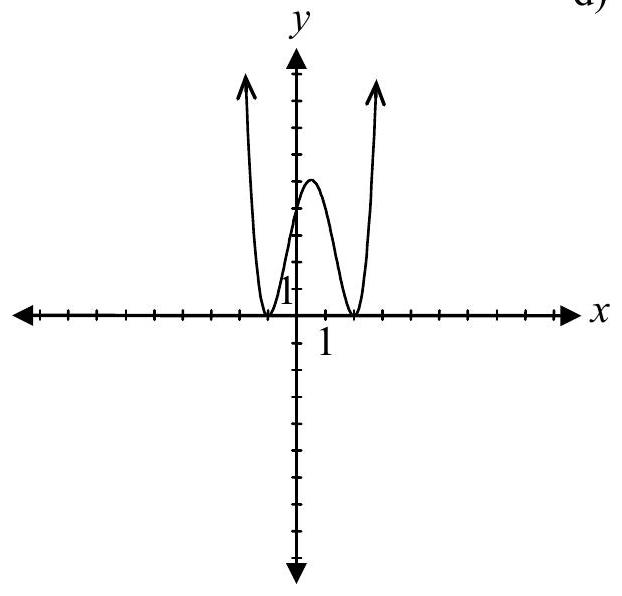
\includegraphics[max width=\textwidth, alt={}, center]{f67fedaf-ea11-42ad-a16e-f30d2fcf2bd3-142_596_622_1216_414}\\
d)\\
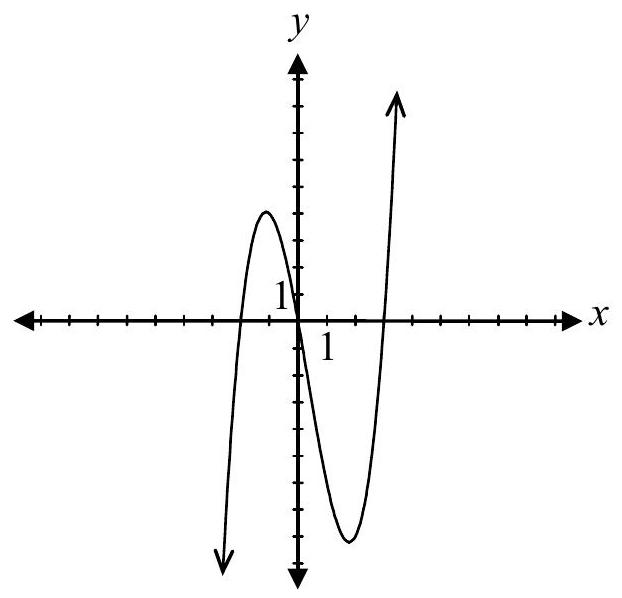
\includegraphics[max width=\textwidth, alt={}, center]{f67fedaf-ea11-42ad-a16e-f30d2fcf2bd3-142_598_622_1211_1155}

A non-permissible value of $x$ for the function $f(x)=\frac{1}{\cos x+1}$ is:\\
a) -1\\
b) 0\\
c) $\pi$\\
d) $\frac{3 \pi}{2}$

Question 21

Identify which of the following statements is true for the rational function $f(x)=\frac{4(x-1)(x-2)}{(x-1)(x+3)}$.\\
a) The equation of the horizontal asymptote is $y=4$.\\
b) The equation of the vertical asymptote is $x=1$.\\
c) The $y$-intercept is 0 .\\
d) There is a point of discontinuity (hole) when $x=2$.

Determine the equation of the polynomial function, $p(x)$, represented by the graph.\\
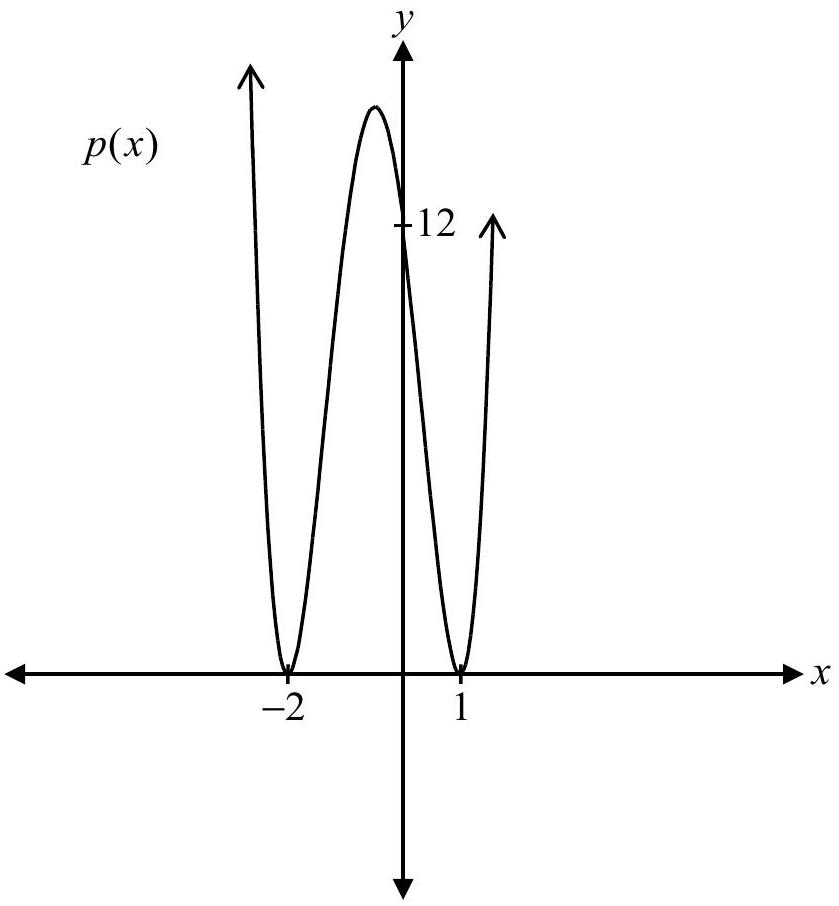
\includegraphics[max width=\textwidth, alt={}, center]{f67fedaf-ea11-42ad-a16e-f30d2fcf2bd3-144_906_839_433_292}

\section*{Solution}
$$
p(x)=3(x+2)^{2}(x-1)^{2}
$$

1 mark for factors\\
1 mark for multiplicity of $2\left(\frac{1}{2}\right.$ mark for each $)$\\
1 mark for correct value of $a$ (consistent with factors and multiplicity)

3 marks

Evaluate:\\
$\log _{4} 2$

\section*{Solution}
$\frac{1}{2}$ □\\
1 mark

Evaluate:

$$
\left(\cos \frac{11 \pi}{3}\right)\left(\csc \frac{11 \pi}{6}\right)
$$

\section*{Solution}
$\left(\frac{1}{2}\right)(-2)$\\
1 mark for $\cos \frac{11 \pi}{3}\left(\frac{1}{2}\right.$ mark for the quadrant, $\frac{1}{2}$ mark for the value)\\
1 mark for $\csc \frac{11 \pi}{6}\left(\frac{1}{2}\right.$ mark for the quadrant, $\frac{1}{2}$ mark for the value)\\
-1

2 marks

Estimate the value of $\log _{2} 5$.\\
Justify your answer.

\section*{Solution}
$\left.\begin{array}{l}\log _{2} 4=2 \\ \log _{2} 8=3\end{array}\right\} \quad 1 / 2$ mark for justification\\
$\therefore \log _{2} 5 \approx 2.3 \quad 1 / 2$ mark for estimated value in the interval $[2.1,2.4]$\\
1 mark

If $\theta$ terminates in quadrant III and $\cos \theta=-\frac{6}{7}$, determine the exact value of $\tan \theta$.

\section*{Solution}
$$
\begin{array}{rlrl}
\cos \theta & =\frac{x}{r} & \\
x^{2}+y^{2} & =r^{2} & & \\
y^{2} & =(7)^{2}-(-6)^{2} & & 1 / 2 \text { mark for substitution of } x=-6 \text { and } r=7 \\
y^{2} & =13 & & \\
y & = \pm \sqrt{13} & & 1 / 2 \text { mark for solving for } y \\
\tan \theta & =\frac{\sqrt{13}}{6} & & 1 \text { mark for the value of } \tan \theta(1 / 2 \text { mark for the quadrant, } 1 / 2 \text { mark for the value })
\end{array}
$$

Given $f(x)=x^{2}+x-4$ and $g(x)=\sqrt{x+5}$, Taz was asked to find $f(g(x))$.\\
Taz's solution:

$$
\begin{aligned}
f(g(x)) & =(\sqrt{x+5})^{2}+x-4 \\
& =x+5+x-4 \\
& =2 x+1, x \geq-5
\end{aligned}
$$

Describe the error in Taz's solution.

\section*{Solution}
Taz must substitute $g(x)$ in both terms containing $x$ in $f(x)$ and then simplify.

Sketch the graph of the function $f(x)=3 \log _{2}(x+1)$.

\section*{Solution}
\begin{center}
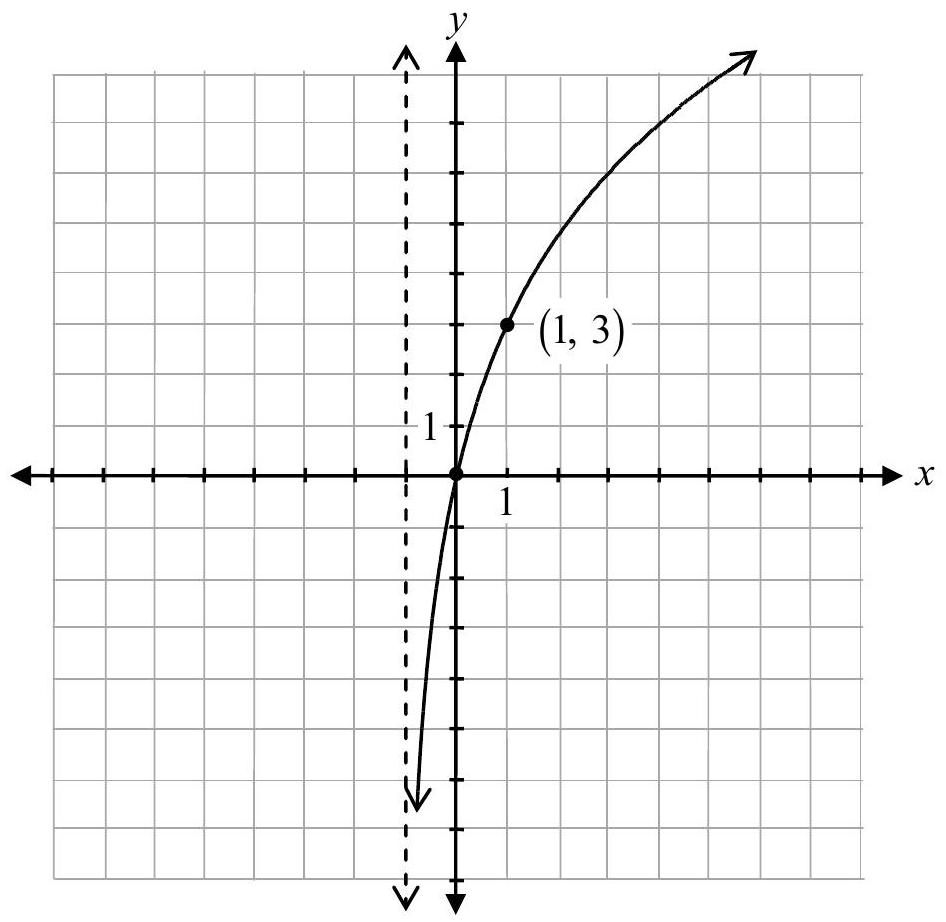
\includegraphics[max width=\textwidth, alt={}]{f67fedaf-ea11-42ad-a16e-f30d2fcf2bd3-150_922_946_580_146}
\end{center}

1 mark for increasing logarithmic function 1 mark for vertical stretch 1 mark for asymptotic behaviour at $x=-1$

Write an equation of a rational function that would not have any vertical asymptotes.

\section*{Solution}
Various equations, such as the following, are possible:

$$
\begin{aligned}
& y=\frac{(x-2)(x+1)}{(x-2)} \\
& \quad \text { or } \\
& y=\frac{4}{x^{2}+4}
\end{aligned}
$$

Determine the exact value of $\tan 75^{\circ}$.

\section*{Solution}
$$
\begin{array}{rlr}
\tan 75^{\circ} & =\tan \left(30^{\circ}+45^{\circ}\right) & 1 \text { mark for combination } \\
& =\frac{\tan 30^{\circ}+\tan 45^{\circ}}{1-\tan 30^{\circ} \tan 45^{\circ}} & 1 \text { mark for exact values }(1 / 2 \text { mark for each }) \\
& =\frac{\frac{1}{\sqrt{3}}+1}{1-\frac{1}{\sqrt{3}}(1)} & \mathbf{2} \text { marks } \\
& =\frac{\frac{1+\sqrt{3}}{\sqrt{3}}}{\frac{\sqrt{3}-1}{\sqrt{3}}} \\
& =\frac{1+\sqrt{3}}{\sqrt{3}-1} \\
& \mathbf{o r} \\
& =\frac{\sqrt{3}+3}{3-\sqrt{3}}
\end{array}
$$

Note(s):

\begin{itemize}
  \item Other combinations are possible.
\end{itemize}

Sketch the graph of the following function:

$$
f(x)=\frac{(x+3)(x-3)}{x(x-3)}
$$

\section*{Solution}
$$
\begin{aligned}
f(x)= & \frac{(x+3)(x /-3)}{x(y-3)} \\
& =\frac{x+3}{x}, x \neq 3
\end{aligned}
$$

∴ there is a point of discontinuity (hole) at $(3,2)$\\
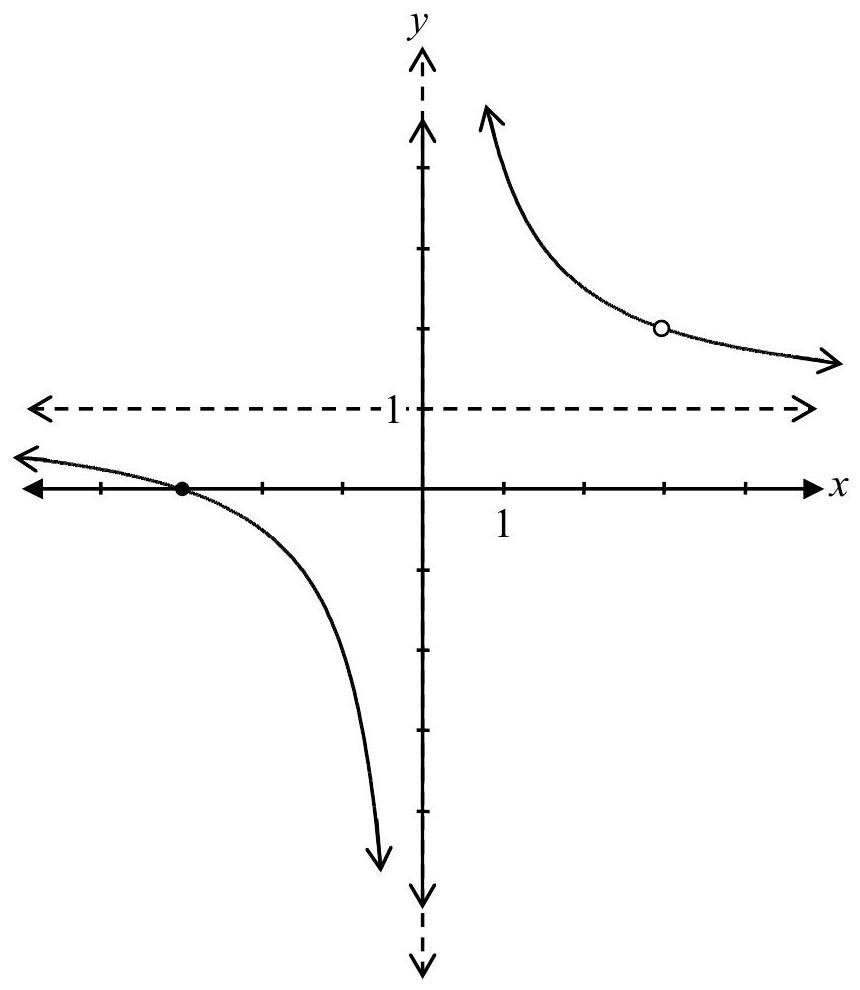
\includegraphics[max width=\textwidth, alt={}, center]{f67fedaf-ea11-42ad-a16e-f30d2fcf2bd3-153_990_860_1052_148}

1 mark for asymptotic behaviour at $y=1$ 1 mark for asymptotic behaviour at $x=0$ 1 mark for point of discontinuity (hole) at $(3,2) \left(\frac{1}{2}\right.$ mark for $x=3, \frac{1}{2}$ mark for $y=2$ ) $\frac{1}{2}$ mark for graph left of vertical asymptote $\frac{1}{2}$ mark for graph right of vertical asymptote

4 marks

In the binomial expansion of $\left(\frac{1}{x^{3}}-2 x^{2}\right)^{9}$, determine which term contains $x^{3}$.

\section*{Solution}
\section*{Method 1}
$$
\begin{aligned}
x^{3} & =\left(x^{-3}\right)^{9-k}\left(x^{2}\right)^{k} \\
x^{3} & =x^{-27+3 k+2 k} \\
3 & =-27+3 k+2 k \\
30 & =5 k \\
6 & =k
\end{aligned}
$$

∴ term 7 would contain $x^{3}$\\
$\frac{1}{2}$ mark for substitution\\
$\frac{1}{2}$ mark for solving for $k$\\
1 mark for identifying the 7th term (or consistent term with the value of $k$ )

\section*{2 marks}
\section*{Method 2}
$\left(\frac{1}{x^{3}}\right)^{9},\left(\frac{1}{x^{3}}\right)^{8}\left(x^{2}\right),\left(\frac{1}{x^{3}}\right)^{7}\left(x^{2}\right)^{2}$\\
$x^{-27}, x^{-22}, x^{-17}$\\
∴ term 7 would contain $x^{3}$

1 mark for determining the pattern\\
1 mark for identifying the 7th term (or consistent term with the pattern)

2 marks

José and Dana get on a Ferris wheel, which is 1 metre off the ground. The diameter of the Ferris wheel is 16 metres. Their ride lasts for 4 minutes, in which time the Ferris wheel makes one revolution.

Determine the values of $\mathrm{A}, \mathrm{B}, \mathrm{C}$, and D , if the sinusoidal function that models the situation is $h(t)=A \cos [B(t-C)]+D$, where $h$ is the height at which José and Dana are located on the Ferris wheel, from the ground, in metres, and $t$ is the time, in minutes.\\
$\mathrm{A}=$ $\_\_\_\_$\\
$\mathrm{B}=$ $\_\_\_\_$\\
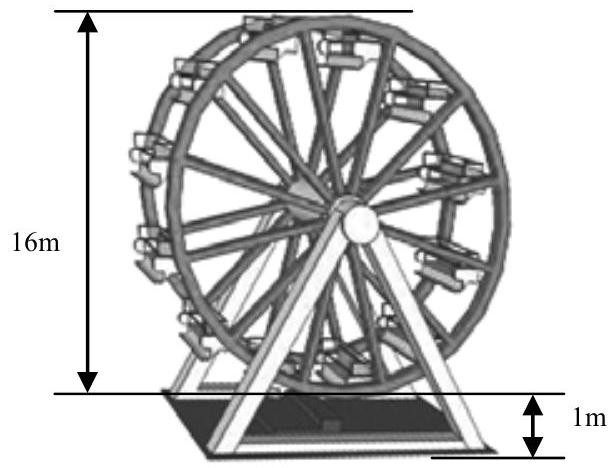
\includegraphics[max width=\textwidth, alt={}, center]{f67fedaf-ea11-42ad-a16e-f30d2fcf2bd3-155_468_614_708_880}\\
$\mathrm{C}=$ $\_\_\_\_$\\
$\mathrm{D}=$ $\_\_\_\_$

\section*{Solution}
$A=$ $\_\_\_\_$ 8\\
or

$$
A=-8
$$

1 mark for $A$\\
$B=\frac{\pi}{2}$\\
$\_\_\_\_$\\
$C=$ $\_\_\_\_$ 0

D = $\_\_\_\_$ 9

1 mark for $C$\\
1 mark for $B$ 1 mark for $D$

4 marks

Note(s)

\begin{itemize}
  \item Other answers are possible.
\end{itemize}

Solve algebraically:

$$
{ }_{n} P_{3}=4!(n-1)
$$

\section*{Solution}
$$
\begin{array}{rlrl}
\frac{n!}{(n-3)!} & =4!(n-1) & & 1 / 2 \text { mark for substitution } \\
\frac{n(n-1)(n-2)(n-3)!}{(n-3)!} & =4!(n-1) & & 1 \text { mark for factorial expansion } \\
n(n-2) & =24 & & 1 / 2 \text { mark for simplification of factorials } \\
n^{2}-2 n-24 & =0 & & \\
(n-6)(n+4) & =0 & & 1 / 2 \text { mark for rejecting extraneous root } \\
n=6 n \geq-4 & & 1 / 2 \text { mark for the value of } n
\end{array}
$$

3 marks

Given $f(x)=\frac{2}{x-1}$, determine the equation of the inverse, $f^{-1}(x)$.

\section*{Solution}
\section*{Method 1}
$$
\begin{aligned}
\text { let } y & =f(x) \\
f(x) & =\frac{2}{x-1} \\
y & =\frac{2}{x-1} \\
x & =\frac{2}{y-1} \\
y-1 & =\frac{2}{x} \\
y & =\frac{2}{x}+1 \\
f^{-1}(x) & =\frac{2}{x}+1
\end{aligned}
$$

1 mark for switching $x$ and $y$ values\\
$\frac{1}{2}$ mark for solving for $y$\\
$1 / 2$ mark for writing equation of $f^{-1}(x)$

\section*{Method 2}
$$
\begin{aligned}
\text { let } y & =f(x) \\
f(x) & =\frac{2}{x-1} \\
y & =\frac{2}{x-1} \\
x & =\frac{2}{y-1}
\end{aligned}
$$

$$
\begin{aligned}
x(y-1) & =2 \\
x y-x & =2 \\
x y & =2+x \\
y & =\frac{2+x}{x}
\end{aligned}
$$

$$
f^{-1}(x)=\frac{2+x}{x}
$$

\section*{2 marks}
1 mark for switching $x$ and $y$ values\\
$\frac{1}{2}$ mark for solving for $y$\\
$1 / 2$ mark for writing equation of $f^{-1}(x)$

\section*{2 marks}
Solve:

$$
4 \log _{3} 2-\frac{1}{3} \log _{3} 8=\log _{3} a
$$

\section*{Solution}
\section*{Method 1}
$$
\begin{aligned}
\log _{3} 2^{4}-\log _{3} 8^{\frac{1}{3}} & =\log _{3} a \\
\log _{3} 16-\log _{3} 2 & =\log _{3} a \\
\log _{3}\left(\frac{16}{2}\right) & =\log _{3} a \\
\log _{3} 8 & =\log _{3} a \\
a & =8
\end{aligned}
$$

1 mark for power law ( $\frac{1}{2}$ mark for each)

1 mark for quotient law

1 mark for equating arguments

\section*{3 marks}
\section*{Method 2}
$$
\begin{aligned}
\log _{3} 2^{4}-\log _{3} 8^{\frac{1}{3}}-\log _{3} a & =0 \\
\log _{3} 16-\log _{3} 2-\log _{3} a & =0 \\
\log _{3}\left(\frac{16}{2 a}\right) & =0 \\
\log _{3}\left(\frac{8}{a}\right) & =0 \\
3^{0} & =\frac{8}{a} \\
1 & =\frac{8}{a} \\
a & =8
\end{aligned}
$$

1 mark for power law ( $\frac{1}{2}$ mark for each)

1 mark for quotient law

1 mark for exponential form\\
3 marks

Sketch the graph of at least one period of the function $y=3 \cos (\pi x)-1$.

\section*{Solution}
\begin{center}
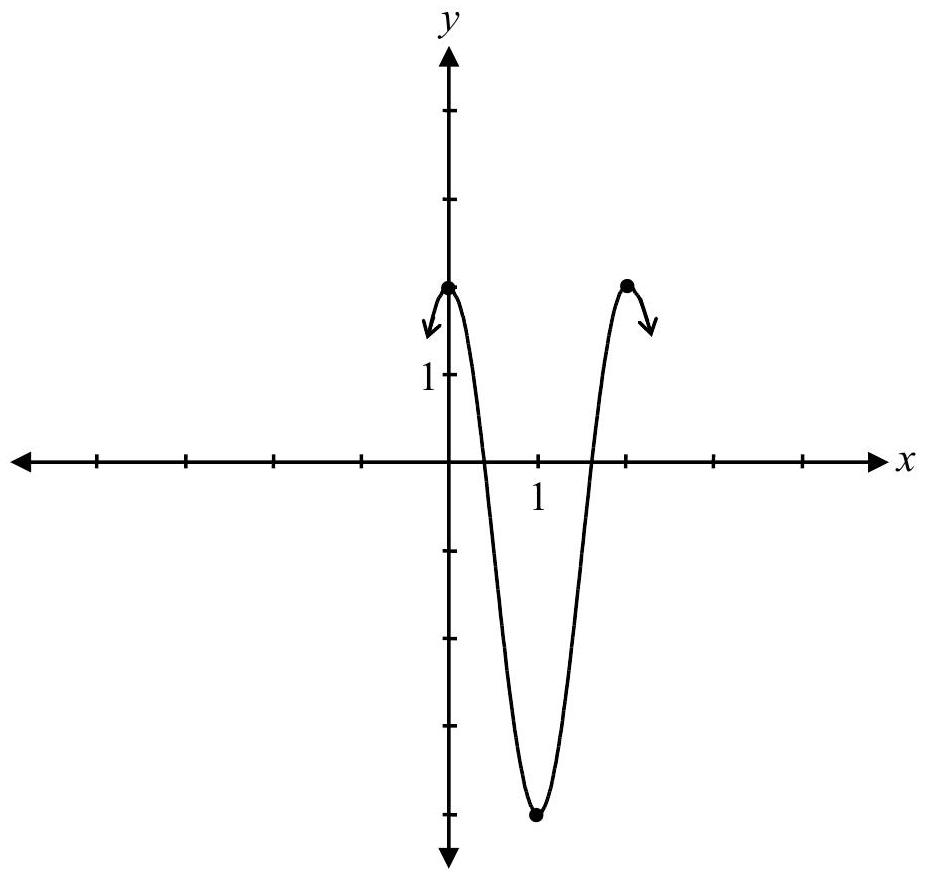
\includegraphics[max width=\textwidth, alt={}]{f67fedaf-ea11-42ad-a16e-f30d2fcf2bd3-159_875_925_610_171}
\end{center}

$$
\begin{aligned}
\text { period } & =\frac{2 \pi}{\pi} \\
& =2
\end{aligned}
$$

1 mark for amplitude\\
1 mark for period\\
1 mark for vertical translation\\
3 marks

Using the laws of logarithms, fully expand the expression:

$$
\log _{a}\left(\frac{x^{3}}{y \sqrt{z}}\right)
$$

\section*{Solution}
$$
\begin{aligned}
\log _{a}\left(\frac{x^{3}}{y \sqrt{z}}\right) & =\log _{a} x^{3}-\left(\log _{a} y+\log _{a} \sqrt{z}\right) \\
& =3 \log _{a} x-\left(\log _{a} y+\frac{1}{2} \log _{a} z\right) \\
& =3 \log _{a} x-\log _{a} y-\frac{1}{2} \log _{a} z
\end{aligned}
$$

1 mark for quotient law\\
1 mark for product law\\
1 mark for power law ( $1 / 2$ mark for each)

Sketch the graph of $f(x)=3 \sqrt{x-2}+1$.

\section*{Solution}
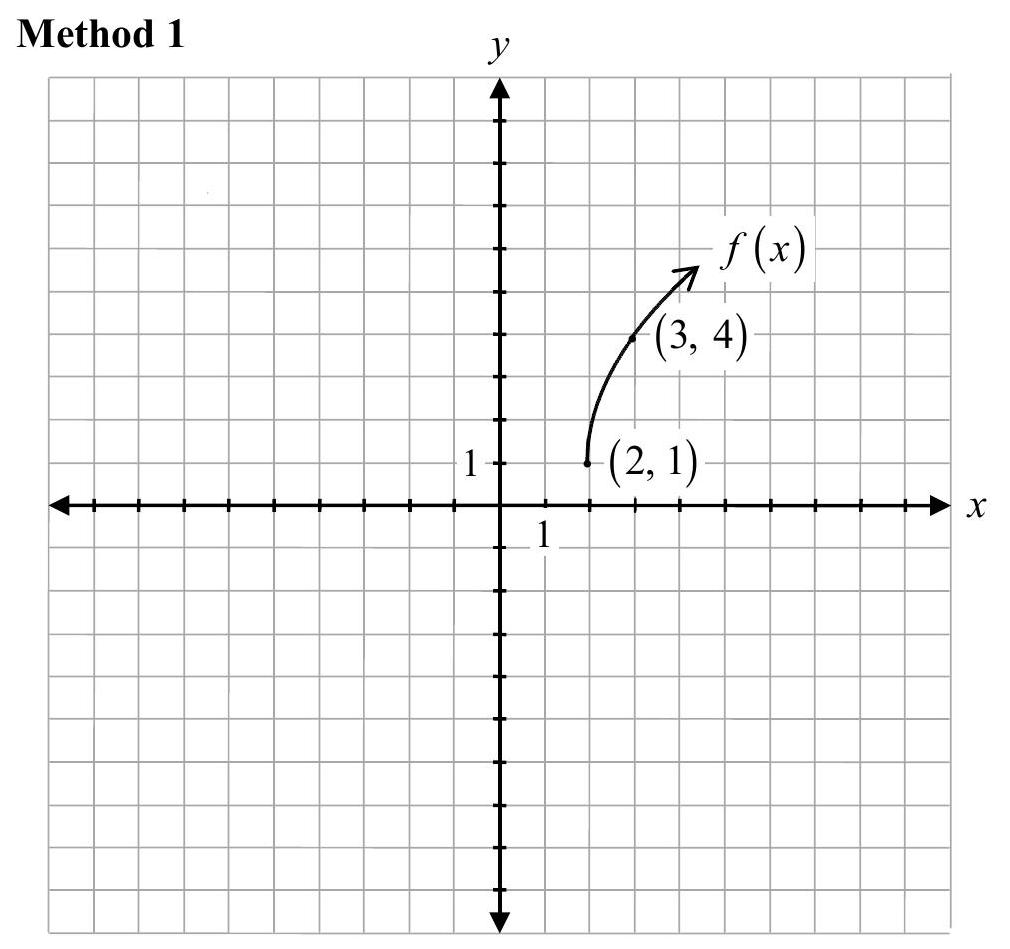
\includegraphics[max width=\textwidth, alt={}, center]{f67fedaf-ea11-42ad-a16e-f30d2fcf2bd3-161_949_1010_575_161}\\
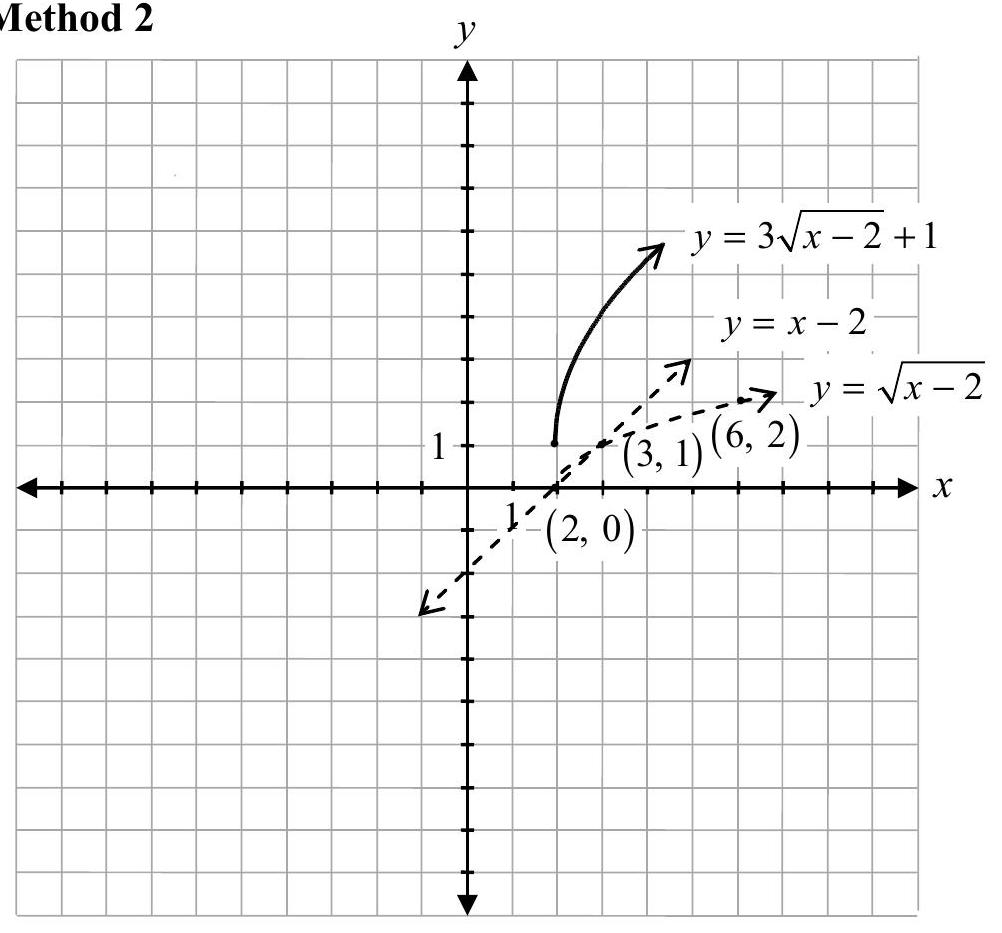
\includegraphics[max width=\textwidth, alt={}, center]{f67fedaf-ea11-42ad-a16e-f30d2fcf2bd3-161_933_1002_1549_193}

1 mark for horizontal translation 1 mark for vertical translation 1 mark for shape of a radical function 1 mark for vertical stretch

1 mark for invariant points where $y=0$ and $y=1$ ( $\frac{1}{2}$ mark for each point) 1 mark for domain $[2, \infty) \frac{1}{2}$ mark for shape between invariant points $\frac{1}{2}$ mark for shape to the right of the invariant points 1 mark for applying transformations ( $\frac{1}{2}$ mark for vertical stretch, $\frac{1}{2}$ mark for vertical translation)\\
a) Determine the domain of the graph of the function $f(x)=\sqrt{x^{2}-4}$.\\
b) Explain why the domain of $f(x)=\sqrt{x^{2}-4}$ is restricted.

\section*{Solution}
a) $\{x \mid x \leq-2 \cup x \geq 2\}$

$$
\begin{gathered}
\text { or } \\
\mathrm{D}:(-\infty,-2] \cup[2, \infty)
\end{gathered}
$$

1 mark for domain ( $\frac{1}{2}$ mark for $x \leq-2,1 / 2$ mark for $x \geq 2$ )\\
b) The domain is restricted because you cannot take the square root of a negative number.

Given the point $(-12,-18)$ on the graph of $f(x)$, determine the new points after the following transformations of $f(x)$.\\
a) $\frac{1}{f(x)}$\\
b) $f(-x)+10$

\section*{Solution}
a) $\left(-12, \frac{-1}{18}\right)$\\
b) $(12,-8)$ 1 mark ( $\frac{1}{2}$ mark for $x$-value, $\frac{1}{2}$ mark for $y$-value $)$

Explain why there is no solution for the equation $\csc \theta=-\frac{1}{2}$.

\section*{Solution}
The value of $\csc \theta$ cannot be between -1 and 1 .\\
or\\
The value of $\sin \theta$ cannot be less than -1 .

Given the graph of $y=f(x)$,\\
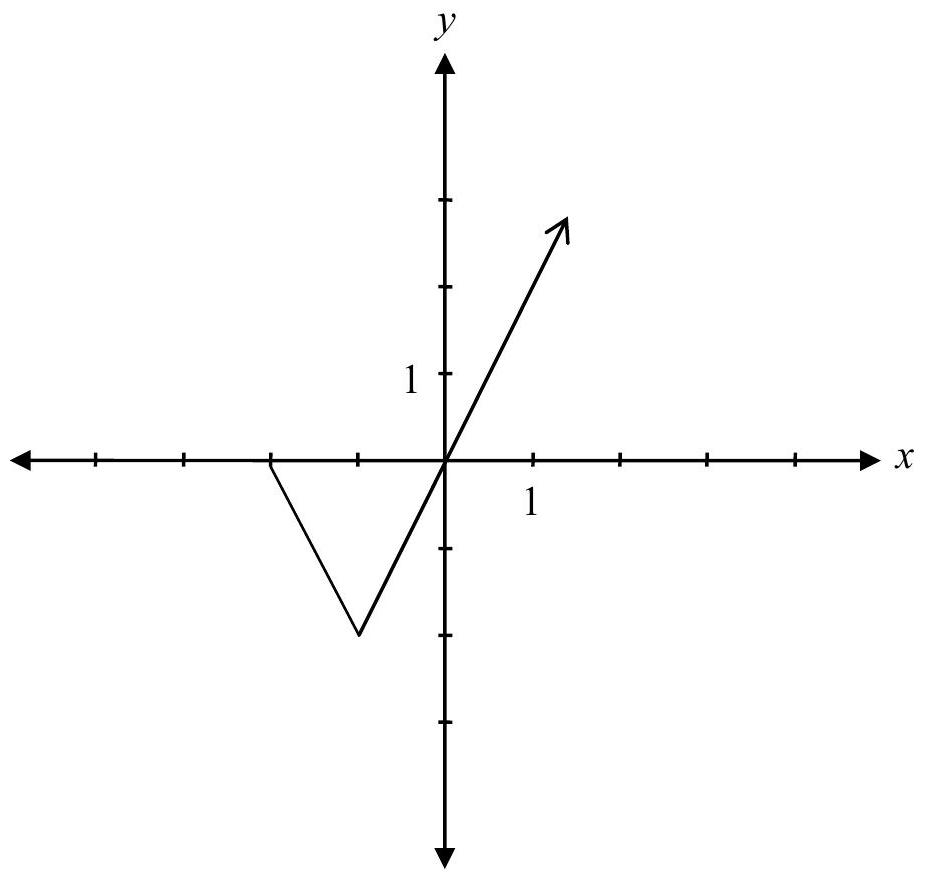
\includegraphics[max width=\textwidth, alt={}, center]{f67fedaf-ea11-42ad-a16e-f30d2fcf2bd3-165_880_927_472_262}\\
sketch the graph of $y=|f(2 x)|+1$.

\section*{Solution}
\begin{center}
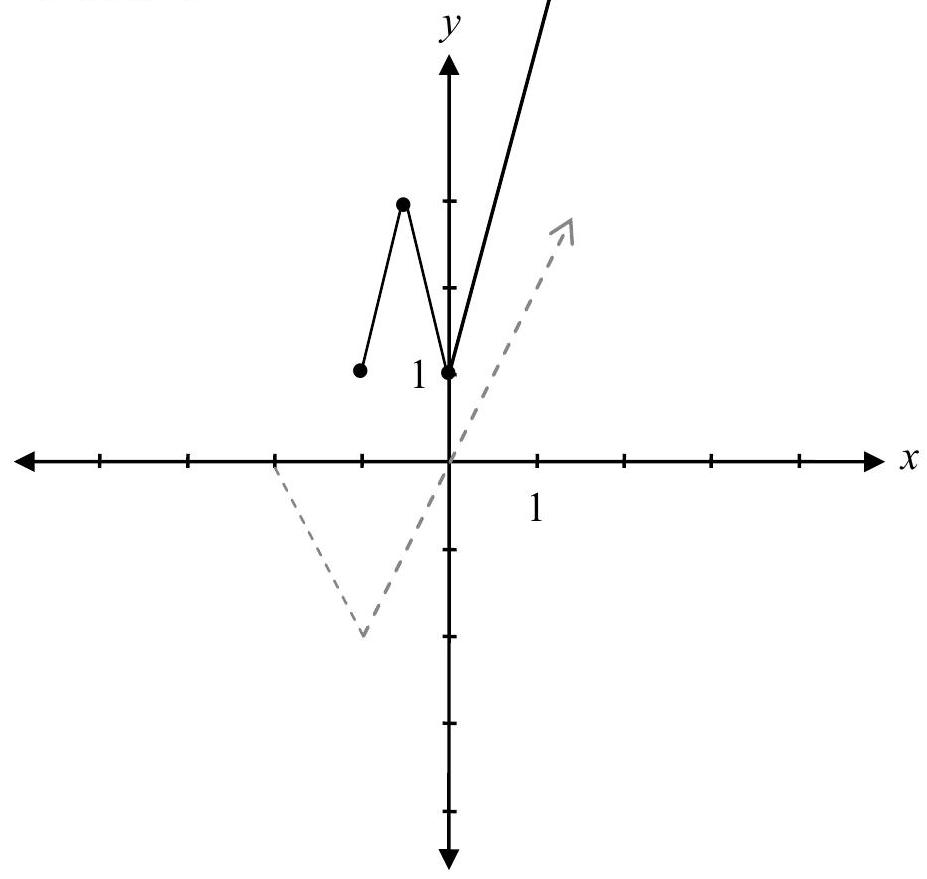
\includegraphics[max width=\textwidth, alt={}]{f67fedaf-ea11-42ad-a16e-f30d2fcf2bd3-165_879_927_1607_171}
\end{center}

1 mark for absolute value 1 mark for horizontal compression 1 mark for vertical translation

Given $f(x)=2^{x}+1$, state the equation of the horizontal asymptote.

\section*{Solution}
$y=1$\\
1 mark

Given the following graphs of $f(x)=x-3$ and $g(x)=x+1$,\\
$f(x)$\\
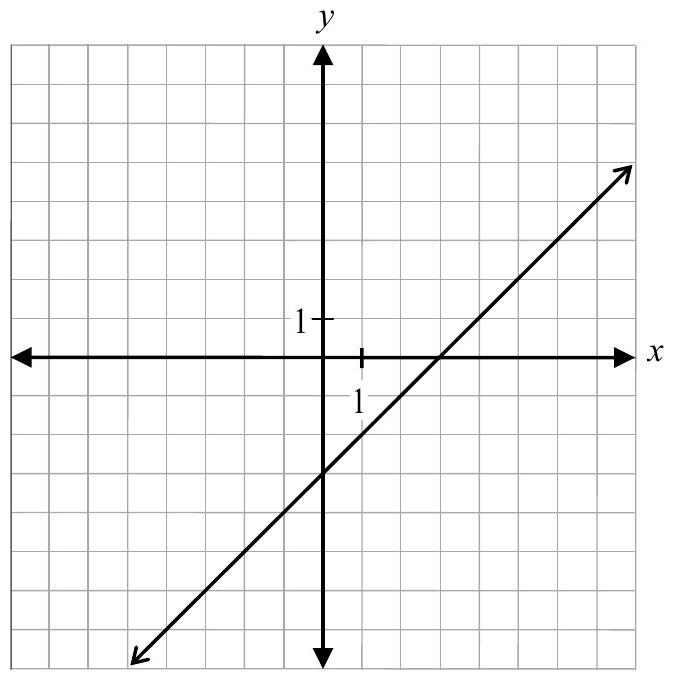
\includegraphics[max width=\textwidth, alt={}, center]{f67fedaf-ea11-42ad-a16e-f30d2fcf2bd3-167_680_674_528_199}\\
$g(x)$\\
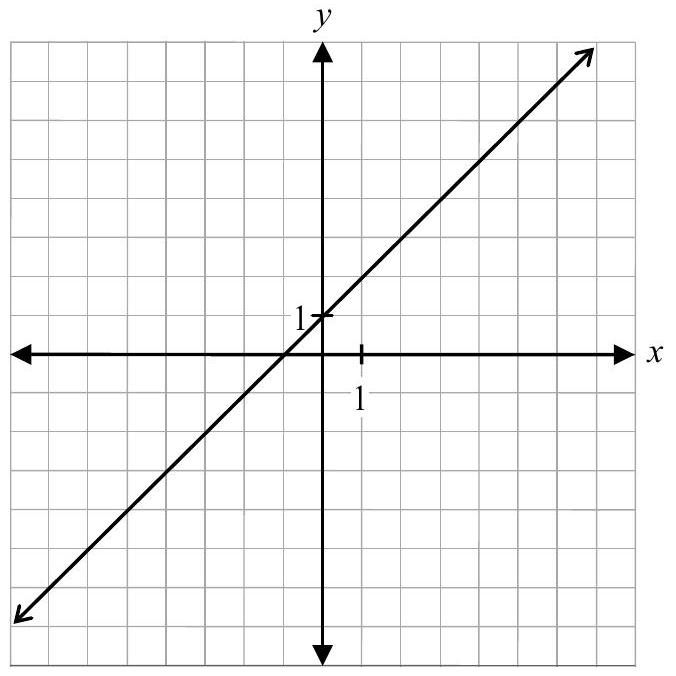
\includegraphics[max width=\textwidth, alt={}, center]{f67fedaf-ea11-42ad-a16e-f30d2fcf2bd3-167_676_676_532_1048}\\
sketch the graph of $h(x)=(f \cdot g)(x)$.

\section*{Solution}
\begin{center}
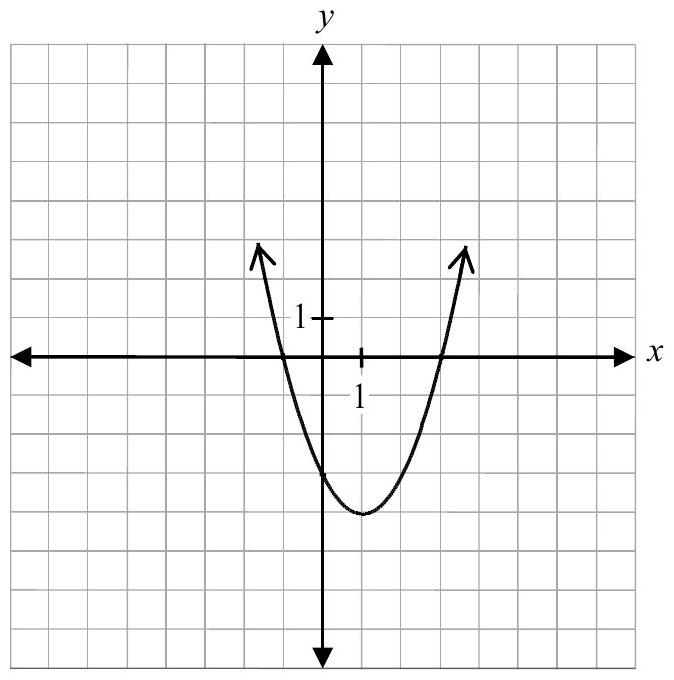
\includegraphics[max width=\textwidth, alt={}]{f67fedaf-ea11-42ad-a16e-f30d2fcf2bd3-167_680_674_1471_199}
\end{center}

1 mark for operation of multiplication 1 mark for shape representing the given operation

\section*{2 marks}
\section*{Question 1}
There are 24 different movies Kiandra can download to her computer. Determine the number of ways she can select 15 movies.

\section*{Solution}
${ }_{24} C_{15}=1307504$ combinations

Given $\theta=40^{\circ}$,\\
a) convert $\theta$ to radians.\\
b) determine the coterminal angles of $\theta$ where $\theta \in \mathbb{R}$.

\section*{Solution}
a)

$$
\begin{gathered}
\theta=40\left(\frac{\pi}{180}\right) \\
\theta=\frac{2 \pi}{9}
\end{gathered}
$$

or

$$
\theta=0.698
$$

b)

$$
\theta=\frac{2 \pi}{9}+2 \pi k \in \mathbb{Z}
$$

or

$$
\theta=0.698+2 \pi k \in \mathbb{Z}
$$

or

$$
\theta=40^{\circ}+360^{\circ} k, k \in \mathbb{Z}
$$

Peter invests $\$ 560$ per month at an annual interest rate of $4.2 \%$, compounded monthly. Determine how many monthly investments he will need to make to obtain at least $\$ 500000$.\\
Express your answer as a whole number.\\
Use the formula:

$$
\mathrm{FV}=\frac{\mathrm{R}\left[(1+i)^{n}-1\right]}{i}
$$

where $\mathrm{FV}=$ the future value

$$
\begin{aligned}
\mathrm{R} & =\text { the investment amount each period } \\
i & =\frac{\text { the annual interest rate }}{\text { the number of compounding periods per year }} \\
n & =\text { the number of investments }
\end{aligned}
$$

\section*{Solution}
$$
\begin{aligned}
500000 & =\frac{560\left[\left(1+\frac{0.042}{12}\right)^{n}-1\right]}{\frac{0.042}{12}} \\
500000 & =\frac{560\left[(1+0.0035)^{n}-1\right]}{0.0035} \\
500000 & =160000\left(1.0035^{n}-1\right) \\
3.125 & =1.0035^{n}-1 \\
4.125 & =1.0035^{n}
\end{aligned}
$$

$$
\log 4.125=\log 1.0035^{n} \quad 1 / 2 \text { mark for applying logarithms }
$$

$\log 4.125=n \log 1.0035 \quad 1$ mark for power law

$$
\begin{array}{rlr}
n= & \frac{\log 4.125}{\log 1.0035} & \\
& n=405.584 & \\
& \therefore 406 \text { monthly investments are needed. } & \\
& \mathbf{3} \text { mark for solving for } n
\end{array}
$$

Ishmael has 4 dogs, 5 cats, and 3 horses.\\
If he arranges all of them in a row, determine how many ways they can be arranged if each type of animal must be grouped together.

\section*{Solution}
$\frac{3!}{\text { types }} \cdot \frac{4!}{\text { dogs }} \cdot \frac{5!}{\text { cats }} \cdot \frac{3!}{\text { horses }}=103680$ ways 1 mark for arrangement of types of animals\\
of\\
animals

Solve the following equation algebraically over the interval $0 \leq \theta \leq 2 \pi$.

$$
2 \cos ^{2} \theta+9 \cos \theta-5=0
$$

\section*{Solution}
$2 \cos ^{2} \theta+9 \cos \theta-5=0$\\
$(2 \cos \theta-1)(\cos \theta+5)=0$\\
$\cos \theta=\frac{1}{2} \quad \cos \theta=-5 \quad 1$ mark for solving for $\cos \theta$\\
$\theta=\frac{\pi}{3}, \frac{5 \pi}{3} \quad$ no solution $\quad \begin{aligned} & 2 \text { marks for solving for } \theta \\ & (1 / 2 \text { mark for each value }, 1\end{aligned}$\\
3 marks

Determine which term contains $\frac{1}{x^{6}}$ in the binomial expansion of $\left(\frac{2}{x^{3}}+3 x^{2}\right)^{7}$.

\section*{Solution}
\section*{Method 1}
$$
\begin{aligned}
\left(x^{-3}\right)^{7-k}\left(x^{2}\right)^{k} & =x^{-6} \\
x^{-21+3 k} x^{2 k} & =x^{-6} \\
x^{-21+5 k} & =x^{-6} \\
-21+5 k & =-6 \\
5 k & =15 \\
k & =3
\end{aligned}
$$

∴ the fourth term contains $\frac{1}{x^{6}}$\\
$\frac{1}{2}$ mark for substitution\\
$\frac{1}{2}$ mark for solving for $k$\\
1 mark for the $4^{\text {th }}$ term (or a term consistent with the value of $k$ )

\section*{2 marks}
\section*{Method 2}
$\left(\frac{1}{x^{3}}\right)^{7},\left(\frac{1}{x^{3}}\right)^{6}\left(x^{2}\right),\left(\frac{1}{x^{3}}\right)^{5}\left(x^{2}\right)^{2}, \ldots$\\
$\frac{1}{x^{21}}, \frac{1}{x^{16}}, \frac{1}{x^{11}}, \ldots$\\
∴ the fourth term contains $\frac{1}{x^{6}}$

1 mark for determining a pattern

1 mark for the $4{ }^{\text {th }}$ term (or a term consistent with the pattern)

\section*{2 marks}
Determine the radius of a circle which has an arc length of 5 cm with a central angle of 3 radians.

\section*{Solution}
$s=\theta r$\\
$5=3 r$\\
$r=\frac{5}{3} \mathrm{~cm}$ □\\
1 mark

Tyler incorrectly sketched the angle $\theta=-\frac{7 \pi}{4}$ in standard position.\\
Describe his error.\\
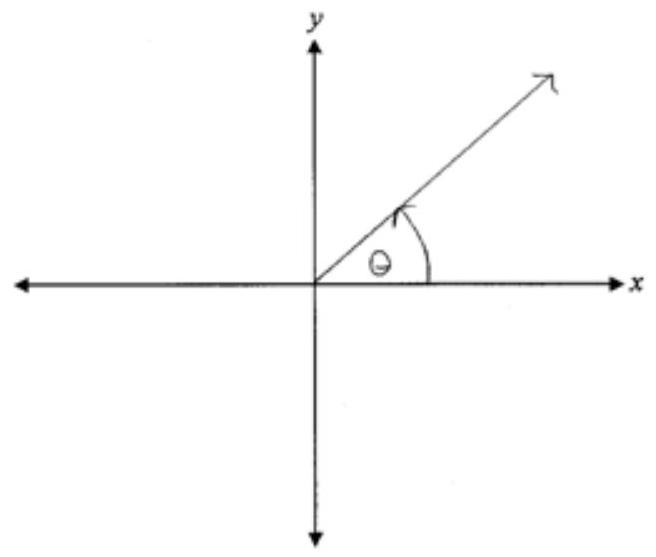
\includegraphics[max width=\textwidth, alt={}, center]{f67fedaf-ea11-42ad-a16e-f30d2fcf2bd3-175_557_656_730_249}

\section*{Solution}
Tyler incorrectly indicated the direction of the angle as positive.\\
or\\
Tyler sketched the reference angle, not $\theta=-\frac{7 \pi}{4}$.

Given the identity $\sec \theta+\cos \theta=\frac{2-\sin ^{2} \theta}{\cos \theta}$,\\
a) determine the non-permissible values of $\theta$, over the interval $0 \leq \theta \leq 2 \pi$.\\
b) prove the identity for all permissible values of $\theta$.

\section*{Solution}
a) $\cos \theta=0$

$$
\theta=\frac{\pi}{2}, \frac{3 \pi}{2}
$$

1 mark for non-permissible values\\
( $\frac{1}{2}$ mark for each value)

\section*{Solution}
Method 1\\
b)

\begin{center}
\begin{tabular}{c|c}
Left-Hand Side & Right-Hand Side \\
\hline
$\sec \theta+\cos \theta$ & $\frac{2-\sin ^{2} \theta}{\cos \theta}$ \\
\hline
\end{tabular}
\end{center}

1 mark for correct substitution of appropriate identities

1 mark for algebraic strategies

1 mark for logical process to prove the identity\\
3 marks

\section*{Method 2}
\begin{center}
\begin{tabular}{|l|l|}
\hline
Left-Hand Side & Right-Hand Side \\
\hline
$\sec \theta+\cos \theta$ & \( \begin{aligned} & \frac{2-\sin ^{2} \theta}{\cos \theta} \\ & \frac{2-\left(1-\cos ^{2} \theta\right)}{\cos \theta} \\ & \frac{1+\cos ^{2} \theta}{\cos \theta} \\ & \frac{1}{\cos \theta}+\frac{\cos ^{2} \theta}{\cos \theta} \\ & \sec \theta+\cos \theta \end{aligned} \) \\
\hline
\end{tabular}
\end{center}

Expand using the laws of logarithms.

$$
\log \left(\frac{a}{b^{4}}\right)
$$

\section*{Solution}
$\log a-\log b^{4}$\\
1 mark for quotient law\\
$\log a-4 \log b$\\
1 mark for power law\\
2 marks

State the equation of $g(x)$ in terms of $f(x)$.\\
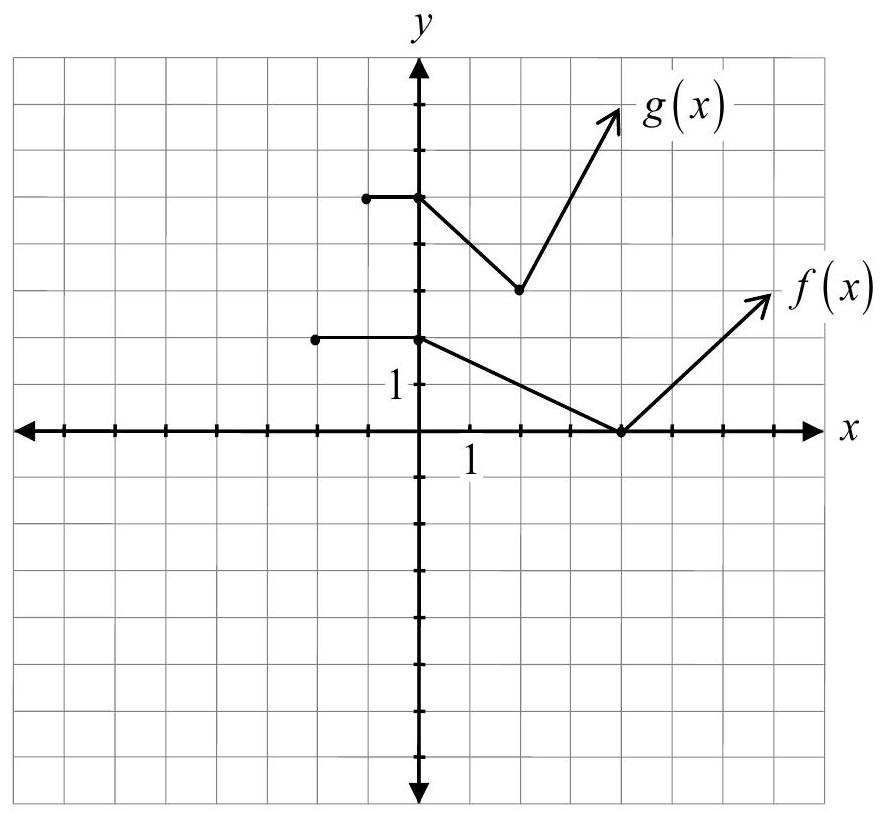
\includegraphics[max width=\textwidth, alt={}, center]{f67fedaf-ea11-42ad-a16e-f30d2fcf2bd3-179_813_888_470_197}

\section*{Solution}
$g(x)=f(2 x)+3$\\
1 mark for horizontal compression\\
1 mark for vertical translation\\
2 marks

Explain why the inverse of the graph of $y=f(x)$ is not a function.\\
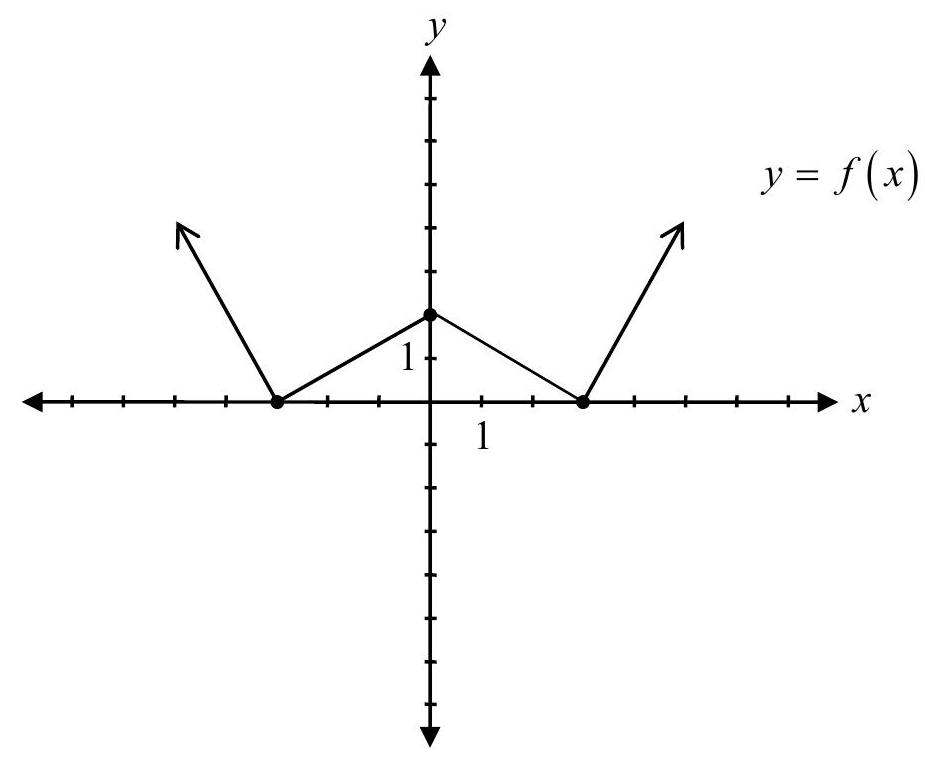
\includegraphics[max width=\textwidth, alt={}, center]{f67fedaf-ea11-42ad-a16e-f30d2fcf2bd3-180_766_933_451_251}

\section*{Solution}
The domain of $f(x)$ was not restricted to ensure there is only one value of $y$ for each $x$ and one value of $x$ for each $y$.

\section*{or}
The graph of the inverse will not pass the vertical line test.

\section*{or}
The graph of $f(x)$ does not pass the horizontal line test.

Solve the following equation algebraically:

$$
\log \left(x^{2}+5\right)-\log \left(x^{2}+1\right)=\log 3
$$

\section*{Solution}
$$
\begin{aligned}
\log \left(\frac{x^{2}+5}{x^{2}+1}\right) & =\log 3 \\
\frac{x^{2}+5}{x^{2}+1} & =3 \\
x^{2}+5 & =3\left(x^{2}+1\right) \\
x^{2}+5 & =3 x^{2}+3 \\
2 & =2 x^{2} \\
1 & =x^{2} \\
\pm 1 & =x
\end{aligned}
$$

1 mark for quotient law\\
$\frac{1}{2}$ mark for equating arguments\\
$\frac{1}{2}$ mark for solving for $x$\\
2 marks

Describe the transformations used to obtain the graph of the function $y=5 f(x+1)$ from the graph of $y=f(x)$.

\section*{Solution}
Vertically stretch the graph by a factor of 5 and translate the graph one unit left.\\
1 mark for vertical stretch\\
1 mark for horizontal translation\\
2 marks

Solve algebraically:

$$
{ }_{n} C_{2}=3 n+4
$$

\section*{Solution}
$$
\begin{aligned}
\frac{n!}{(n-2)!2!} & =3 n+4 \\
\frac{n(n-1)(n-2)!}{(n-2)!} & =2!(3 n+4) \\
n(n-1) & =2(3 n+4) \\
n^{2}-n & =6 n+8 \\
n^{2}-7 n-8 & =0 \\
(n-8)(n+1) & =0 \\
n=8 \quad n>-1 &
\end{aligned}
$$

$\frac{1}{2}$ mark for substitution into equation\\
1 mark for factorial expansion\\
$\frac{1}{2}$ mark for simplification of factorials\\
$\frac{1}{2}$ mark for rejecting the extraneous root $\frac{1}{2}$ mark for the value of $n$

3 marks

Given the graph of $f(x)$, sketch the graph of $y=\left|\frac{1}{2} f(x-1)\right|$.\\
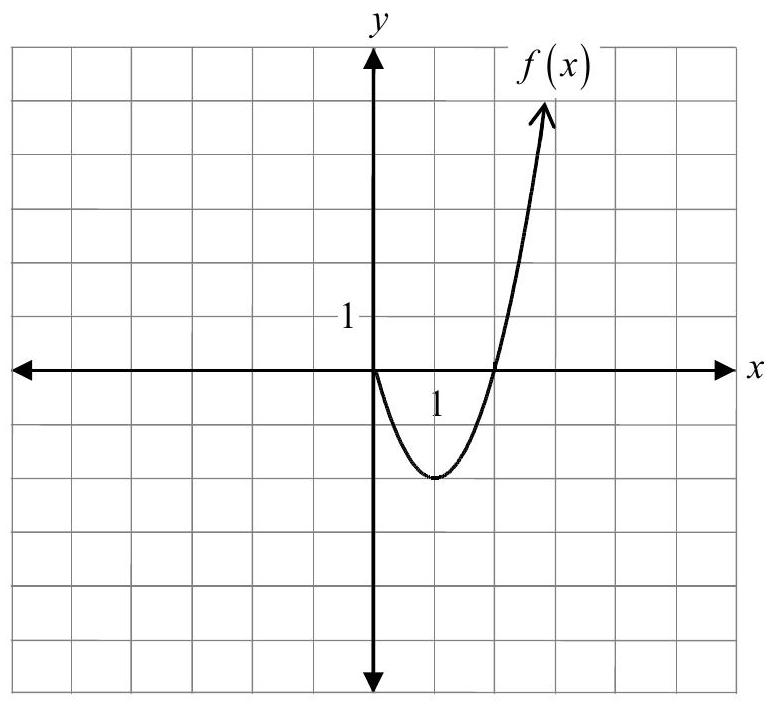
\includegraphics[max width=\textwidth, alt={}, center]{f67fedaf-ea11-42ad-a16e-f30d2fcf2bd3-184_704_775_491_227}

\section*{Solution}
\begin{center}
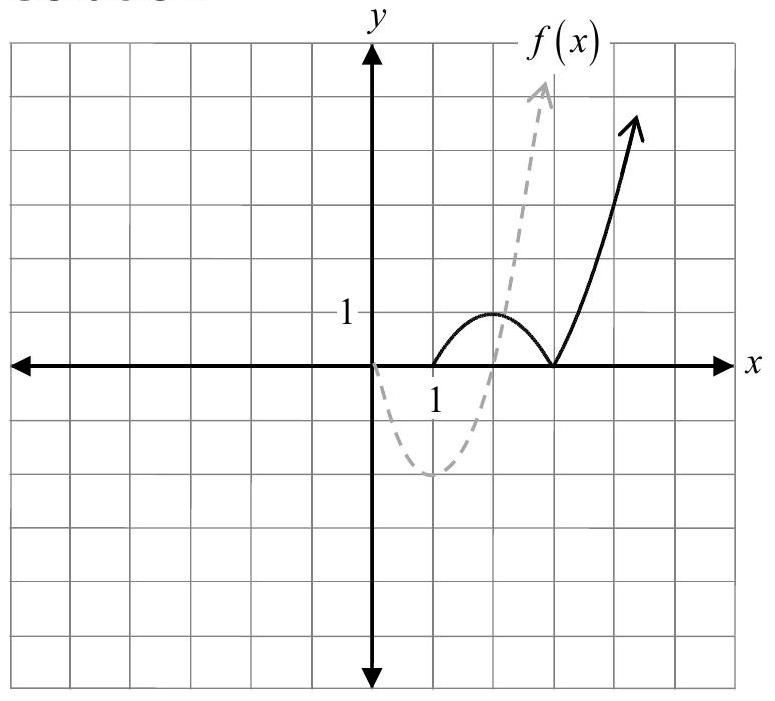
\includegraphics[max width=\textwidth, alt={}]{f67fedaf-ea11-42ad-a16e-f30d2fcf2bd3-184_701_775_1295_199}
\end{center}

1 mark for vertical stretch\\
1 mark for horizontal translation\\
1 mark for absolute value

Explain why $f(x)=(x+2)^{3}(x-1)^{\frac{1}{2}}$ is not a polynomial function.

\section*{Solution}
All factors in a polynomial function must have exponents that are whole numbers.

Given the graphs of $f(x)$ and $g(x)$, sketch the graph of $h(x)=(f \cdot g)(x)$.\\
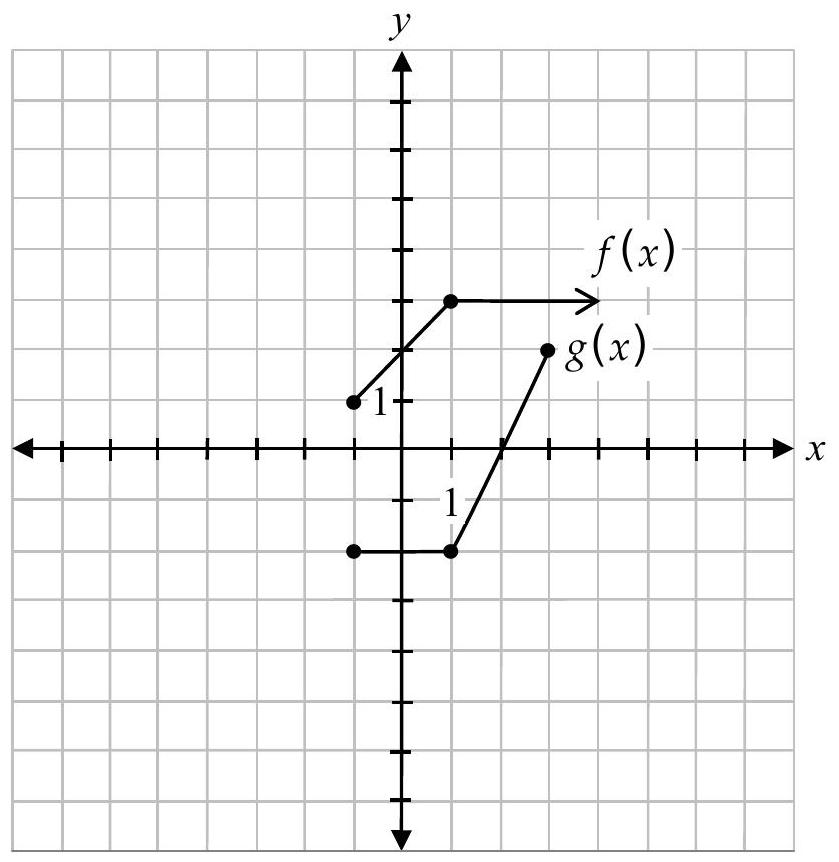
\includegraphics[max width=\textwidth, alt={}, center]{f67fedaf-ea11-42ad-a16e-f30d2fcf2bd3-186_862_839_451_206}

Solution\\
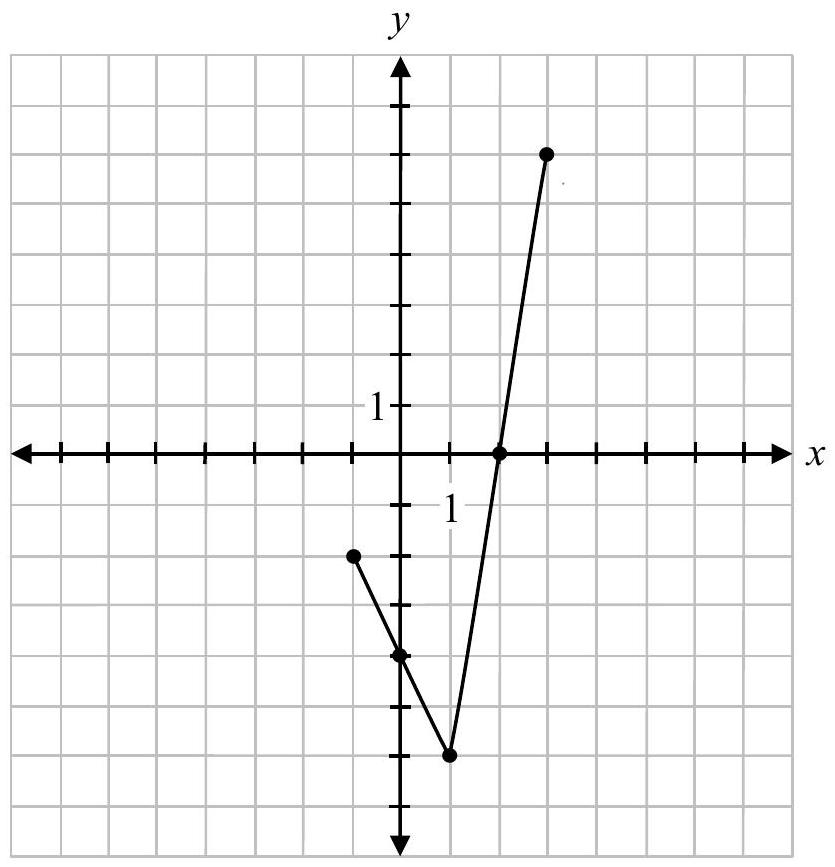
\includegraphics[max width=\textwidth, alt={}, center]{f67fedaf-ea11-42ad-a16e-f30d2fcf2bd3-186_867_835_1503_210}

\begin{center}
\begin{tabular}{r|c|c|c}
$x$ & $f(x)$ & $g(x)$ & $(f \cdot g)(x)$ \\
\hline
-1 & 1 & -2 & -2 \\
1 & 3 & -2 & -6 \\
3 & 3 & 2 & 6 \\
\end{tabular}
\end{center}

1 mark for operation of multiplication 1 mark for restricted domain

Identify the trigonometric function that is equivalent to $\sin \frac{\pi}{4} \cos \frac{\pi}{3}+\cos \frac{\pi}{4} \sin \frac{\pi}{3}$.\\
a) $\quad \sin \frac{2 \pi}{7}$\\
b) $\quad \sin \frac{7 \pi}{12}$\\
c) $\quad \cos \frac{2 \pi}{7}$\\
d) $\quad \cos \frac{7 \pi}{12}$

Question 20

Identify the logarithmic form of $5^{x}=6$.\\
a) $\log _{5} x=6$\\
b) $\log _{5} 6=x$\\
c) $\log _{6} x=5$\\
d) $\log _{6} 5=x$

Given $f(\theta)=3 \cos 2 \theta-1$ and $g(\theta)=\sin \theta+1$, identify which statement is true.\\
a) Both functions have the same period.\\
b) Both functions have the same amplitude.\\
c) Both functions have the same minimum value.\\
d) Both functions have the same maximum value.

Question 22

Identify the fourth term in the expansion of $(x+y)^{5}$.\\
a) $10 x^{4} y$\\
b) $10 x^{3} y^{2}$\\
c) $10 x^{2} y^{3}$\\
d) $10 x y^{4}$

Given the graphs of $f(x)$ and $g(x)$, identify the choice with all of the solutions of the equation $f(x)=g(x)$.\\
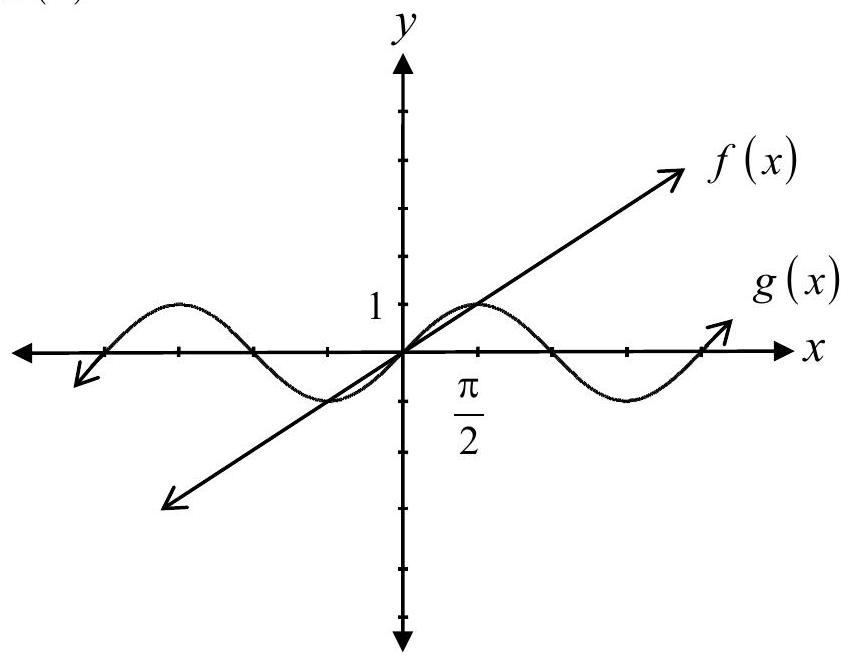
\includegraphics[max width=\textwidth, alt={}, center]{f67fedaf-ea11-42ad-a16e-f30d2fcf2bd3-189_665_854_476_343}\\
a) $\quad x=-2 \pi,-\pi, 0, \pi, 2 \pi$\\
b) $x=-\frac{\pi}{2}, 0, \frac{\pi}{2}$\\
c) $x=\frac{\pi}{2}$\\
d) $x=-1,0,1$

Identify the graph of $f^{-1}(x)$ if $f(x)=x^{2}-9, x \geq 0$.\\
a)\\
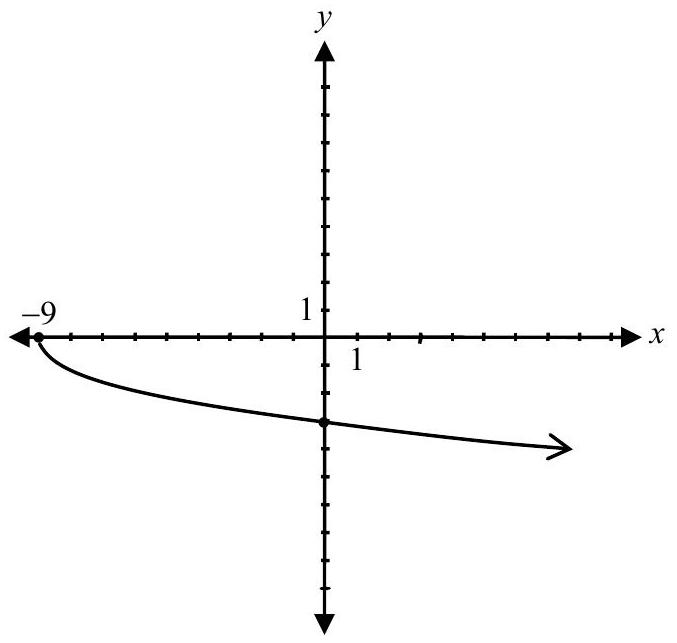
\includegraphics[max width=\textwidth, alt={}, center]{f67fedaf-ea11-42ad-a16e-f30d2fcf2bd3-190_643_677_524_292}\\
b)\\
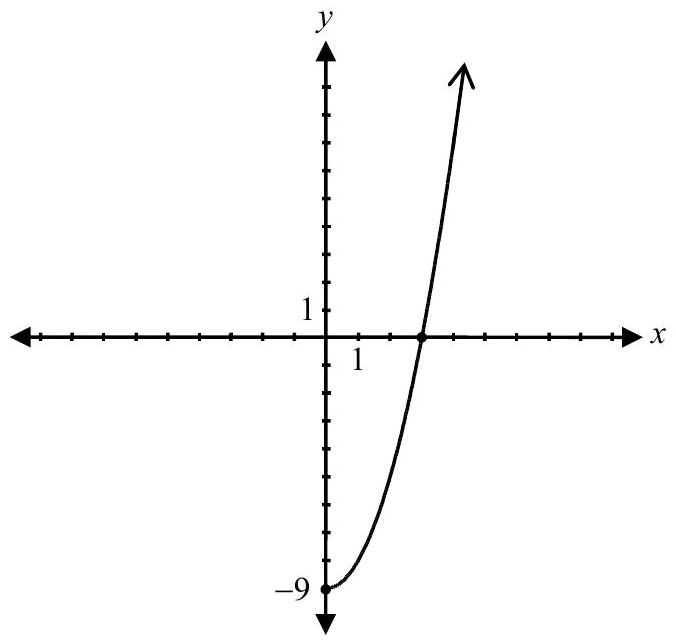
\includegraphics[max width=\textwidth, alt={}, center]{f67fedaf-ea11-42ad-a16e-f30d2fcf2bd3-190_643_676_524_1151}\\
c)\\
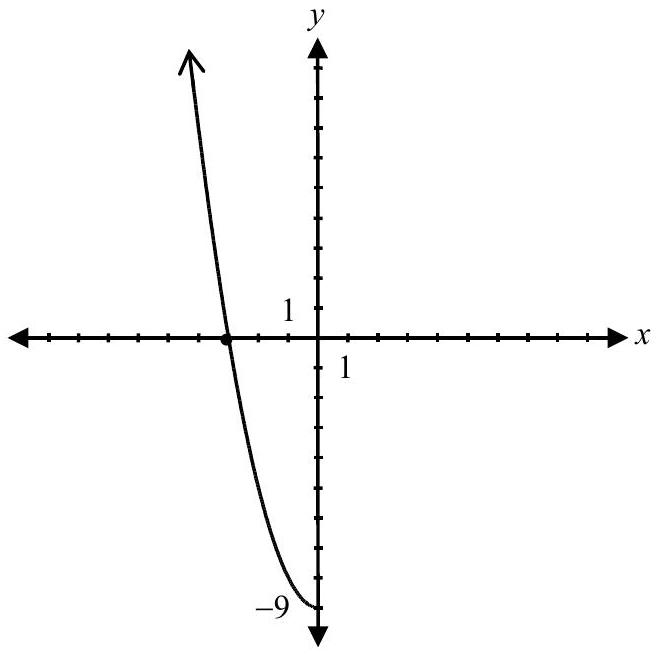
\includegraphics[max width=\textwidth, alt={}, center]{f67fedaf-ea11-42ad-a16e-f30d2fcf2bd3-190_656_661_1383_300}\\
d)\\
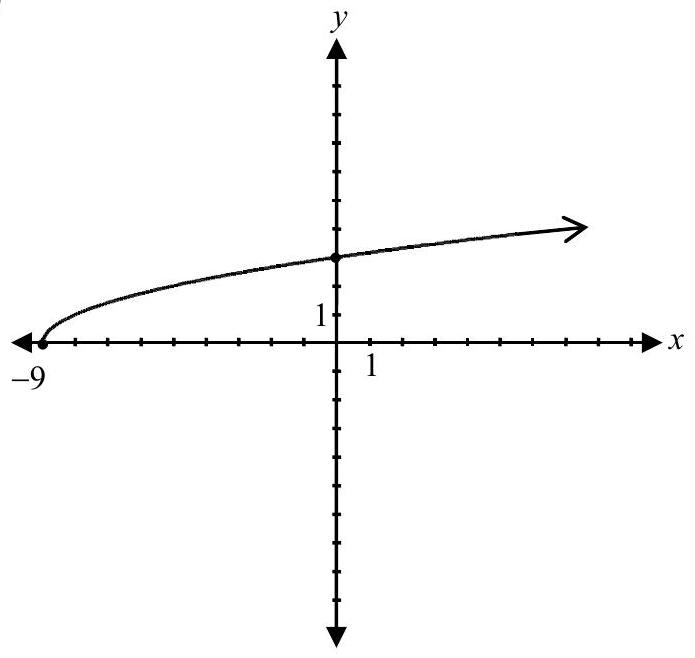
\includegraphics[max width=\textwidth, alt={}, center]{f67fedaf-ea11-42ad-a16e-f30d2fcf2bd3-190_658_695_1377_1149}

Using the remainder theorem, identify which value of $x$ results in a remainder of zero given $p(x)=x^{3}+7 x^{2}+14 x+8$.\\
a) 1\\
b) 0\\
c) -1\\
d) -3

Evaluate $\cos \left(\cos \left(\frac{3 \pi}{2}\right)\right)$.\\
a) 1\\
b) $\frac{1}{2}$\\
c) 0\\
d) -1

Match the following equations with their graphs:

\section*{Solution \\
 Place the appropriate letter in this column.}
$$
\begin{array}{ll}
f(x)=(x-1)^{3}(x+1)(x-3) & \text { C } \\
g(x)=(x+1)^{2}(x-1)(x+3) & \text { B } \\
h(x)=-2(x-1)^{2}(x+1)(x-3) & \text { A } \\
k(x)=2(x+1)^{2}(x-1)(x+3) & \text { D }
\end{array}
$$

$\frac{1}{2}$ mark for each correct answer

$$
2 \text { marks }
$$

\begin{figure}[h]
\begin{center}
\captionsetup{labelformat=empty}
\caption{A)}
  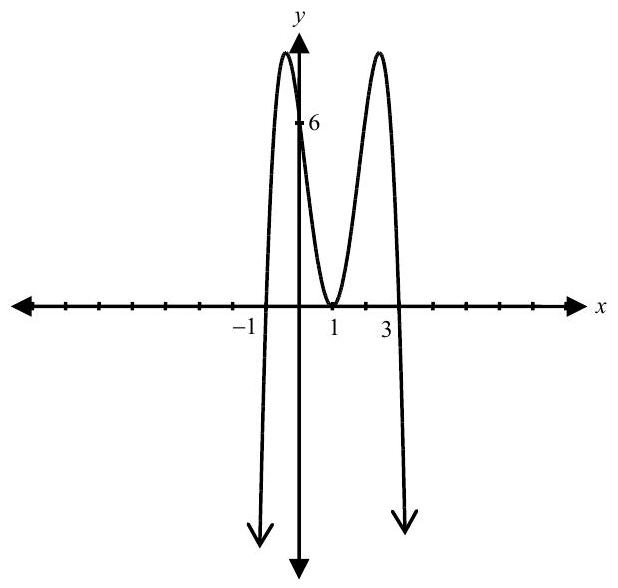
\includegraphics[alt={},max width=\textwidth]{f67fedaf-ea11-42ad-a16e-f30d2fcf2bd3-192_588_618_1181_257}
\end{center}
\end{figure}

\begin{center}
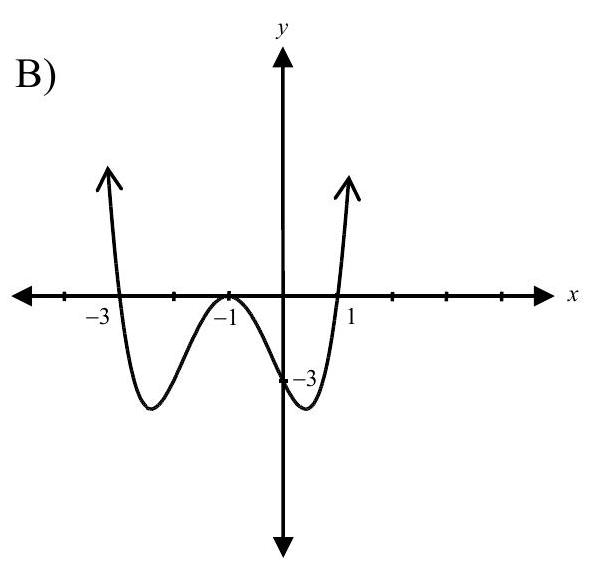
\includegraphics[max width=\textwidth, alt={}]{f67fedaf-ea11-42ad-a16e-f30d2fcf2bd3-192_572_591_1185_1097}
\end{center}

\begin{figure}[h]
\begin{center}
\captionsetup{labelformat=empty}
\caption{C)}
  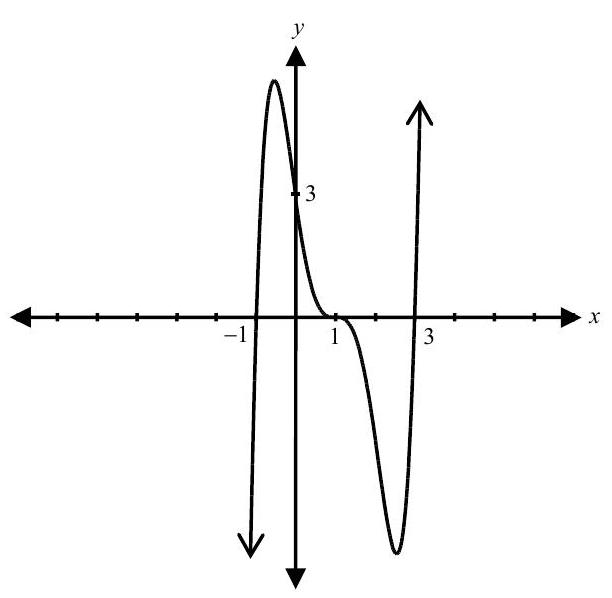
\includegraphics[alt={},max width=\textwidth]{f67fedaf-ea11-42ad-a16e-f30d2fcf2bd3-192_598_612_1873_259}
\end{center}
\end{figure}

\begin{center}
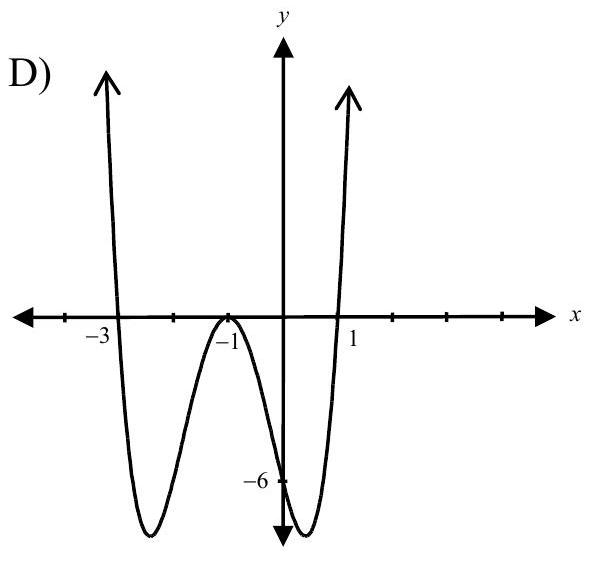
\includegraphics[max width=\textwidth, alt={}]{f67fedaf-ea11-42ad-a16e-f30d2fcf2bd3-192_562_592_1873_1104}
\end{center}

If $\log 6=p, \log 5=r$ and $\log 2=q$, express $\log 60$ in terms of $p, q$ and $r$.

\section*{Solution}
$$
\begin{aligned}
\log 60 & =\log (6 \cdot 5 \cdot 2) & & 1 / 2 \text { mark for combination } \\
& =\log 6+\log 5+\log 2 & & 1 \text { mark for product law } \\
& =p+r+q & & 1 / 2 \text { mark for substitution }
\end{aligned}
$$

Sketch the graph of $y=\sqrt{-2 x}+1$.

\section*{Solution}
\section*{Method 1}
\begin{center}
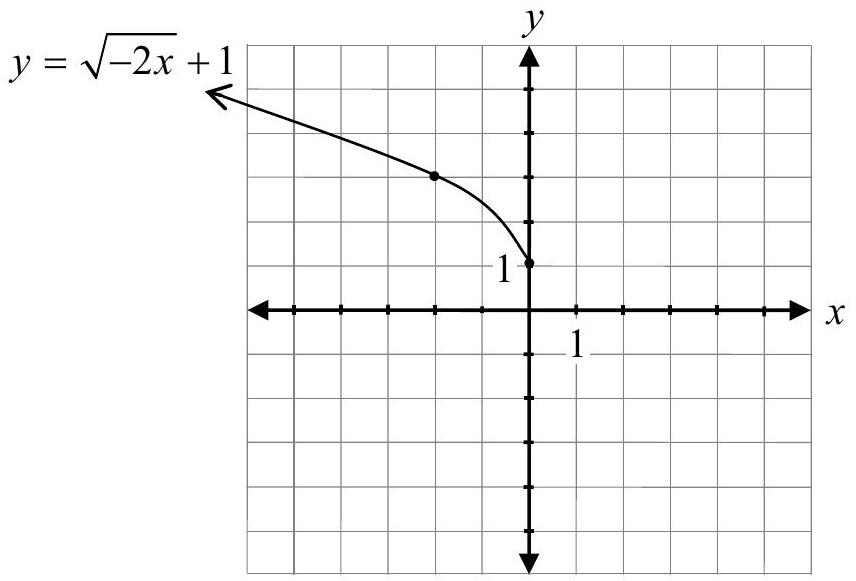
\includegraphics[max width=\textwidth, alt={}]{f67fedaf-ea11-42ad-a16e-f30d2fcf2bd3-194_581_856_676_206}
\end{center}

\section*{Method 2}
$$
\begin{gathered}
y=\sqrt{-2 x}+1 \\
y=\sqrt{-2 x}
\end{gathered}
$$

\begin{center}
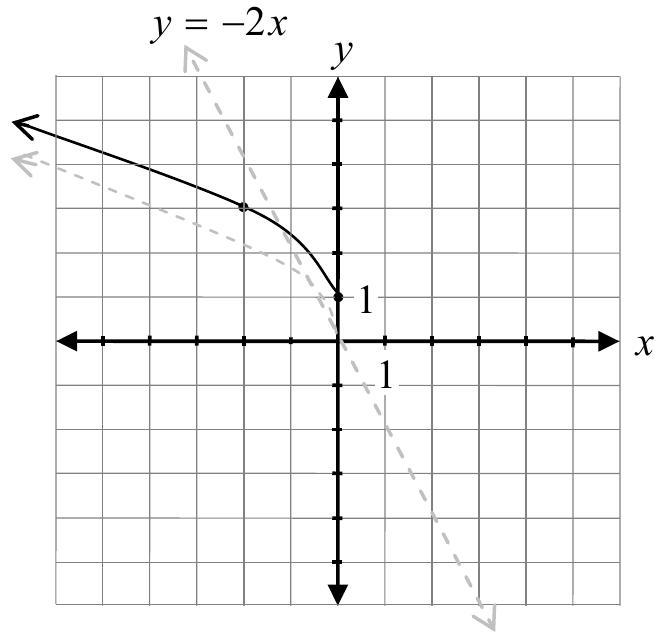
\includegraphics[max width=\textwidth, alt={}]{f67fedaf-ea11-42ad-a16e-f30d2fcf2bd3-194_643_663_1392_416}
\end{center}

1 mark for shape of a radical function 1 mark for horizontal compression\\
1 mark for vertical translation\\
1 mark for horizontal reflection

\section*{4 marks}
$\frac{1}{2}$ mark for shape between invariant points $\frac{1}{2}$ mark for shape to the left of the invariant points 1 mark for invariant points where $y=0$ and $y=1$ ( $\frac{1}{2}$ mark for each point) 1 mark for domain of $(-\infty, 0]$ 1 mark for vertical translation

Justify why the letters of the word FRANCE have a greater number of possible arrangements than the letters of the word CANADA.

\section*{Solution}
CANADA has repeated letters that, when placed in different orders, do not change the arrangements of the letters.

FRANCE: 6 ! CANADA: $\frac{6 \text { ! }}{3 \text { ! }}$\\
∴ France has a greater number of arrangements.

Given $f(x)=\frac{1}{x-2}$ and $g(x)=x+5$,\\
a) determine the equation for $f(g(x))$.\\
b) sketch the graph of $f(g(x))$.

\section*{Solution}
a) $\quad f(g(x))=\frac{1}{(x+5)-2}$\\

\includegraphics[max width=\textwidth, alt={}, center]{f67fedaf-ea11-42ad-a16e-f30d2fcf2bd3-196_130_218_889_1039}

$$
=\frac{1}{x+3}
$$

\begin{center}
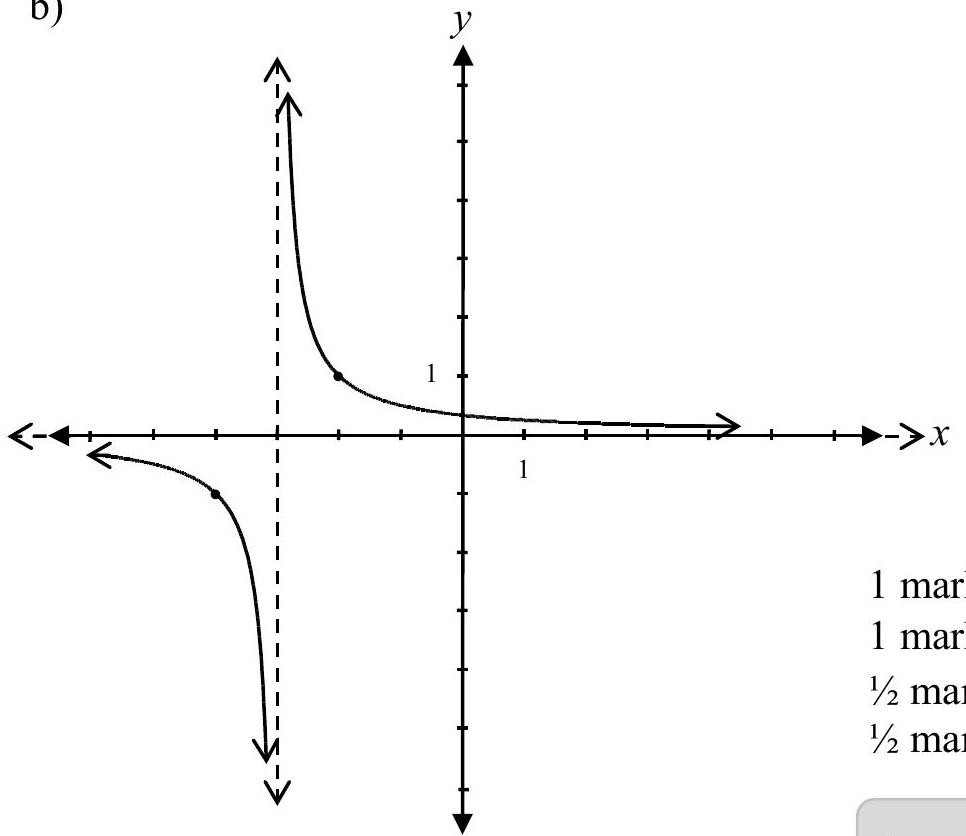
\includegraphics[max width=\textwidth, alt={}]{f67fedaf-ea11-42ad-a16e-f30d2fcf2bd3-196_836_966_1173_180}
\end{center}

1 mark for asymptotic behaviour approaching $x=-3$ 1 mark for asymptotic behaviour approaching $y=0 \frac{1}{2}$ mark for branch left of vertical asymptote $\frac{1}{2}$ mark for branch right of vertical asymptote

Given that $\sin \alpha=\frac{3}{7}$, where $\alpha$ is in Quadrant II, and $\cos \beta=\frac{4}{5}$, where $\beta$ is in Quadrant IV, determine the exact value of:\\
a) $\sin (\alpha-\beta)$

\section*{Solution}
\begin{center}
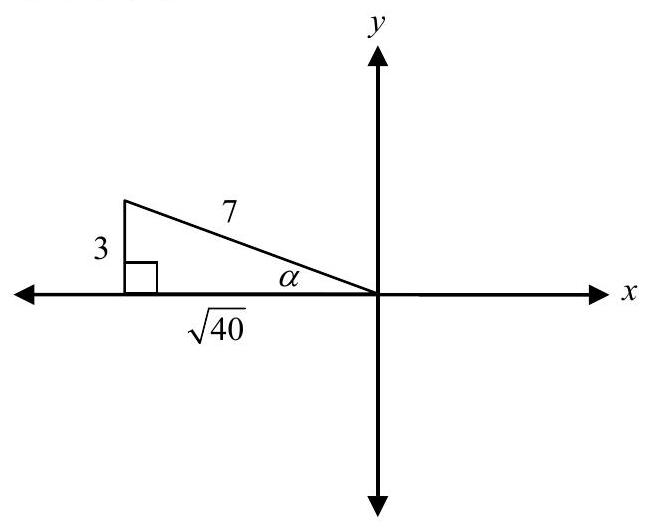
\includegraphics[max width=\textwidth, alt={}]{f67fedaf-ea11-42ad-a16e-f30d2fcf2bd3-197_532_654_734_193}
\end{center}

$$
\begin{aligned}
x^{2}+y^{2} & =r^{2} \\
x^{2}+9 & =49 \\
x^{2} & =40 \\
x & = \pm \sqrt{40} \quad 1 / 2 \text { mark for value of } x
\end{aligned}
$$

\begin{center}
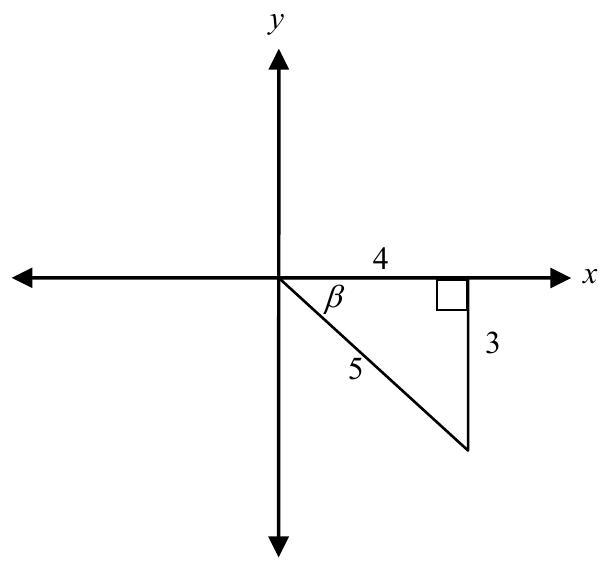
\includegraphics[max width=\textwidth, alt={}]{f67fedaf-ea11-42ad-a16e-f30d2fcf2bd3-197_570_609_1280_296}
\end{center}

$$
\begin{aligned}
x^{2}+y^{2} & =r^{2} \\
16+y^{2} & =25 \\
y^{2} & =9 \\
y & = \pm 3 \quad 1 / 2 \text { mark for value of } y
\end{aligned}
$$

$\sin (\alpha-\beta)=\sin \alpha \cos \beta-\cos \alpha \sin \beta$

$$
\begin{aligned}
& =\left(\frac{3}{7}\right)\left(\frac{4}{5}\right)-\left(\frac{-\sqrt{40}}{7}\right)\left(\frac{-3}{5}\right) \\
& =\frac{12}{35}-\frac{3 \sqrt{40}}{35} \\
& =\frac{12-3 \sqrt{40}}{35} \text { or } \frac{12-6 \sqrt{10}}{35}
\end{aligned}
$$

$\frac{1}{2}$ mark for $\cos \alpha$\\
$\frac{1}{2}$ mark for $\sin \beta$\\
1 mark for substitution into correct identity

\section*{3 marks}
\section*{Note(s):}
\begin{itemize}
  \item accept any of the following values for $x: x= \pm \sqrt{40}, x=-\sqrt{40}$ or $x=\sqrt{40}$
  \item accept any of the following values for $y: y= \pm 3, y=-3$ or $y=3$\\
b) $\cos 2 \alpha$
\end{itemize}

\section*{Solution}
$$
\begin{aligned}
\cos 2 \alpha & =\cos ^{2} \alpha-\sin ^{2} \alpha \\
& =\left(\frac{-\sqrt{40}}{7}\right)^{2}-\left(\frac{3}{7}\right)^{2} \\
& =\frac{40}{49}-\frac{9}{49} \\
& =\frac{31}{49}
\end{aligned}
$$

or

$$
\begin{aligned}
\cos 2 \alpha & =2 \cos ^{2} \alpha-1 \\
& =2\left(\frac{-\sqrt{40}}{7}\right)^{2}-1 \\
& =2\left(\frac{40}{49}\right)-1 \\
& =\frac{80}{49}-1 \\
& =\frac{31}{49}
\end{aligned}
$$

or

$$
\begin{aligned}
\cos 2 \alpha & =1-2 \sin ^{2} \alpha \\
& =1-2\left(\frac{3}{7}\right)^{2} \\
& =1-2\left(\frac{9}{49}\right) \quad 1 \text { mark for substitution of an appropriate identity } \\
& =1-\frac{18}{49} \\
& =\frac{31}{49}
\end{aligned}
$$

Determine the domain and range of $f(x)=\sqrt{x-5}-1$.

\section*{Solution}
Domain: $\{x \in \mathbb{R} \mid x \geq 5\} \quad$ or $\quad[5, \infty) \quad 1$ mark for domain

Range: $\{y \in \mathbb{R} \mid y \geq-1\}$ or $[-1, \infty) \quad 1$ mark for range\\
2 marks

Justify why 4.7 is a better estimate than 4.3 for the value of $\log _{2} 26$.

\section*{Solution}
$$
\begin{gathered}
2^{4}=16 \quad 2^{5}=32 \\
\quad \text { or } \\
\log _{2} 16=4 \quad \log _{2} 32=5
\end{gathered}
$$

26 is closer to 32 than 16 ; therefore $\log _{2} 26$ is closer to 5 than 4 .

Sketch the graph of the function:

$$
f(x)=\frac{x(x-2)(x-4)}{(x-2)}
$$

\section*{Solution}
\begin{center}
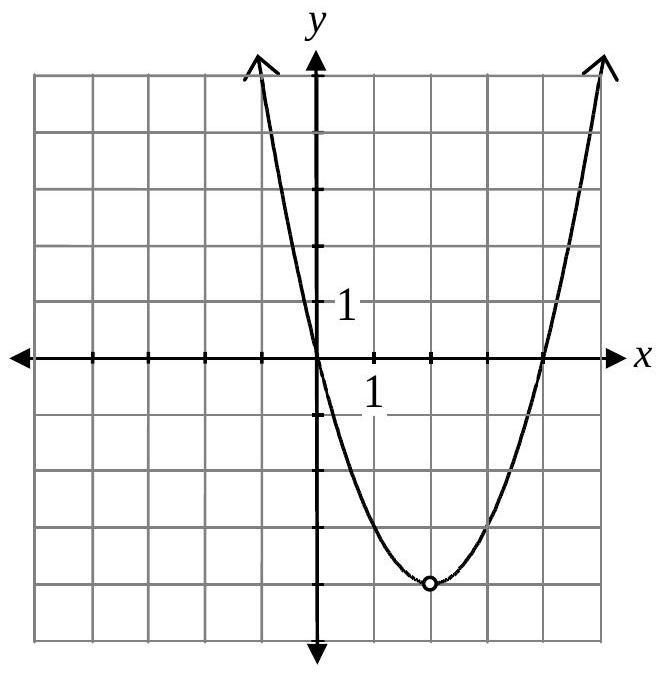
\includegraphics[max width=\textwidth, alt={}]{f67fedaf-ea11-42ad-a16e-f30d2fcf2bd3-201_673_663_730_216}
\end{center}

1 mark for point of discontinuity (hole) at ( $2,-4$ )\\
( $\frac{1}{2}$ mark for $x$ value, $\frac{1}{2}$ mark for $y$ value)\\
$\frac{1}{2}$ mark for shape of a parabola\\
$\frac{1}{2}$ mark for end behaviour\\
2 marks

Evaluate:

$$
\sec ^{2}\left(\frac{\pi}{6}\right)+\tan \left(\frac{7 \pi}{6}\right) \csc \left(-\frac{2 \pi}{3}\right)
$$

\section*{Solution}
$\left(\frac{2}{\sqrt{3}}\right)^{2}+\left(\frac{\sqrt{3}}{3}\right)\left(-\frac{2}{\sqrt{3}}\right.$\\
$\left(\frac{4}{3}\right)-\left(\frac{2}{3}\right)$\\
$\frac{2}{3}$

1 mark for $\sec \left(\frac{\pi}{6}\right)(1 / 2$ mark for value, $1 / 2$ mark for quadrant)\\
1 mark for $\tan \left(\frac{7 \pi}{6}\right)(1 / 2$ mark for value, $1 / 2$ mark for quadrant)\\
1 mark for $\csc \left(-\frac{2 \pi}{3}\right)(1 / 2$ mark for value, $1 / 2$ mark quadrant $)$ 3 marks

The graph of $f(x)=3 x+7$ is reflected over the $y$-axis.\\
Determine the equation of the new function.

\section*{Solution}
$$
y=-3 x+7
$$

or

$$
y=f(-x)
$$

Determine the equations of all of the asymptotes of the function:

$$
y=\frac{2 x+1}{x-3}
$$

\section*{Solution}
\begin{center}
\begin{tabular}{ll}
Horizontal asymptote at $y=2$ & 1 mark for horizontal asymptote \\
Vertical asymptote at $x=3$ & 1 mark for vertical asymptote \\
 & $\mathbf{2}$ marks \\
\end{tabular}
\end{center}

One of the zeros of $p(x)=x^{3}+6 x^{2}-32$ is $x=2$. Determine all of the other zeros of $p(x)$.

\section*{Solution}
\begin{center}
\begin{tabular}{r|rrrr}
2 & 1 & 6 & 0 & -32 \\
 & $\downarrow$ & 2 & 16 & 32 \\
\hline
 & 1 & 8 & 16 & 0 \\
\hline
\end{tabular}
\end{center}

1 mark for synthetic division (or any equivalent strategy)

$$
\begin{aligned}
& 0=x^{2}+8 x+16 \\
& 0=(x+4)(x+4) \\
& x=-4
\end{aligned}
$$

$\frac{1}{2}$ mark for the other factors\\
$\frac{1}{2}$ mark for the other zeros\\
2 marks

Sketch the graph of $y=-2^{x}+2$.

\section*{Solution}
\begin{center}
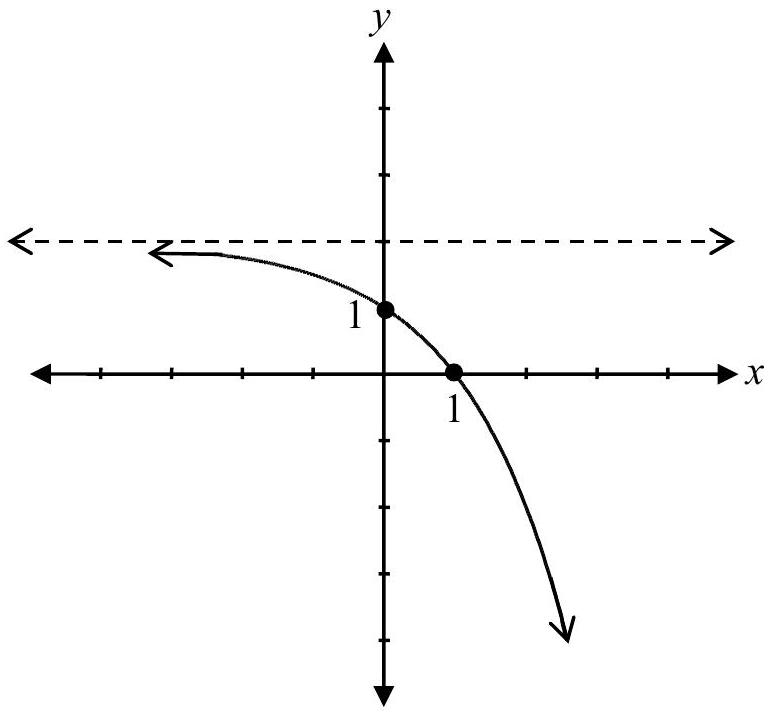
\includegraphics[max width=\textwidth, alt={}]{f67fedaf-ea11-42ad-a16e-f30d2fcf2bd3-206_712_774_601_236}
\end{center}

1 mark for shape of an exponential function 1 mark for vertical reflection\\
1 mark for asymptotic behaviour approaching $y=2$

Given the function $f(x)=\frac{2}{x}-1$, justify why $f(f(2))$ is undefined.

\section*{Solution}
$$
\begin{aligned}
f(2) & =\frac{2}{2}-1 \\
& =1-1 \\
& =0
\end{aligned}
$$

$f(f(2))=\frac{2}{0}-1$, which is undefined because the denominator cannot be zero.

1 mark for justification\\
1 mark

The following graph represents the volume of air in an adult's lungs. If $V(t)$ is the volume of air in litres and $t$ is the time in seconds, determine an equation that represents this sinusoidal function.\\
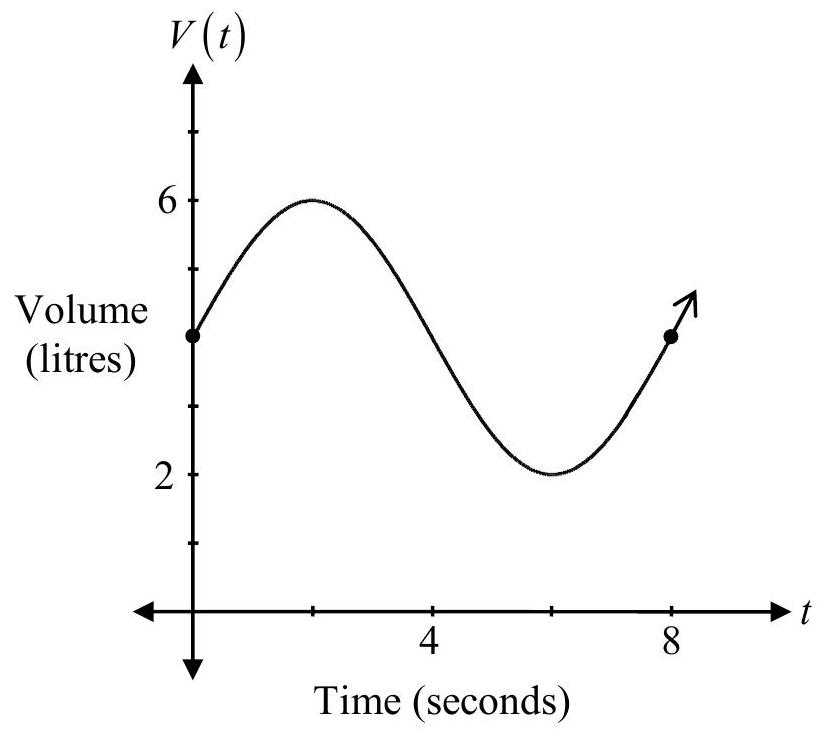
\includegraphics[max width=\textwidth, alt={}, center]{f67fedaf-ea11-42ad-a16e-f30d2fcf2bd3-208_735_828_550_214}

\section*{Solution}
$V(t)=2 \sin \left(\frac{\pi}{4} t\right)+4$\\
or\\
1 mark for amplitude\\
$\frac{1}{2}$ mark for period\\
$\frac{1}{2}$ mark for consistent value of $b$\\
1 mark for vertical translation\\
$V(t)=2 \cos \left[\frac{\pi}{4}(t-2)\right]+4$\\
3 marks

Explain why the domain of $y=\log _{2}(x-1)$ is $x>1$.

\section*{Solution}
The argument of a logarithmic function must be positive.

The point ( $-2,7$ ) is on the terminal arm of an angle in standard position.\\
Determine the coordinates of the corresponding point, $P(\theta)$, on the unit circle.

\section*{Solution}
$$
\begin{array}{rlrl}
x^{2}+y^{2} & =r^{2} & & \\
(-2)^{2}+(7)^{2} & =r^{2} & & 1 / 2 \text { mark for substitution of } x= \pm 2 \text { and } y=7 \\
4+49 & =r^{2} & & \\
53 & =r^{2} & 1 / 2 \text { mark for solving for } r \\
\sqrt{53} & =r & 1 \text { mark for } P(\theta)\left(\frac{1}{2} \text { mark for each coordinate }\right) \\
P(\theta) & =\left(\frac{-2}{\sqrt{53}}, \frac{7}{\sqrt{53}}\right) & 1 \text { marks }
\end{array}
$$

Sketch a graph of $P(x)$ that satisfies all of the following conditions:

\begin{itemize}
  \item $P(x)$ is a polynomial function of degree 3 .
  \item $P(x)$ has a zero at -3 with a multiplicity of 2 .
  \item $P(x)$ has a zero at 1 .
  \item $P(x)$ has a leading coefficient of -3 .
\end{itemize}

\section*{Solution}
\begin{center}
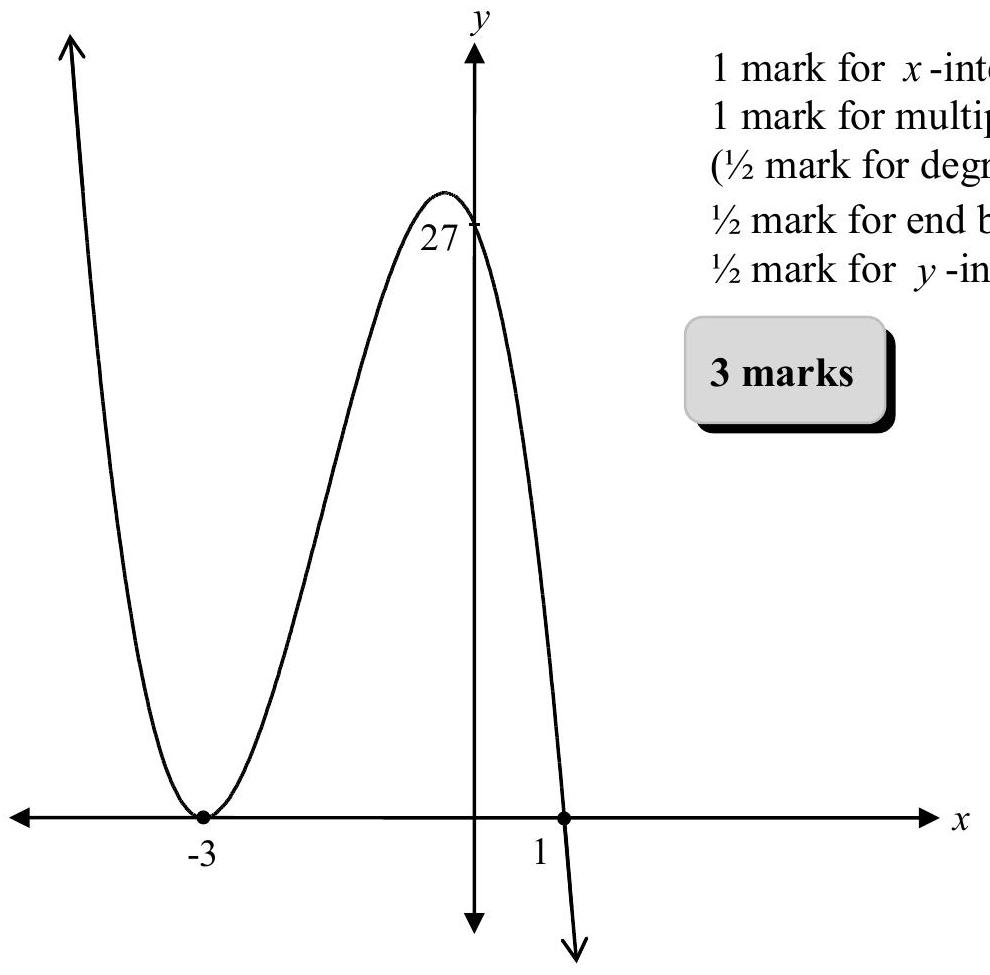
\includegraphics[max width=\textwidth, alt={}]{f67fedaf-ea11-42ad-a16e-f30d2fcf2bd3-211_975_990_858_197}
\end{center}

Determine how many 4-digit numbers greater than 4000 can be made using the digits $2,3,4,5$, and 6 if repetitions are not allowed.

\section*{Solution}
$\frac{3}{4,5,6} \cdot \frac{4}{\text { remaining options }}=72$

1 mark for restriction of first digit\\
1 mark for fundamental counting principle\\
2 marks

A group of 7 friends decide to go to a movie.\\
Determine how many ways the friends can sit in a row if two of the friends refuse to sit next to each other.

\section*{Solution}
$7!-6!2!=3600$ ways

$$
\begin{aligned}
& \frac{1}{2} \text { mark for } 7! \\
& 1 \text { mark for product of } 6!2! \\
& \left(\frac{1}{2} \text { mark for } 6!, 1 / 2 \text { mark for } 2!\right) \\
& 1 / 2 \text { mark for subtraction } \\
& \mathbf{2} \text { marks }
\end{aligned}
$$

Gabrielle listens to her radio at a sound level of 80 dB . She attended a music concert that had a sound level of 115 dB . Determine how many times more intense the music concert was than the radio.

You may use the formula:

$$
\beta=10 \log \left(\frac{I}{I_{0}}\right)
$$

where $\beta$ is the intensity level of sound, measured in dB\\
$\boldsymbol{I}$ is the intensity of sound\\
$I_{0}$ is the standard minimum intensity that a person can hear

\section*{Solution}
Radio:\\
$80=10 \log \left(\frac{I}{I_{0}}\right)$\\
$8=\log \left(\frac{I}{I_{0}}\right)$\\
$10^{8}=\frac{I}{I_{0}} \quad 1 / 2$ mark for exponential form\\
$10^{8} I_{0}=I$\\
$\frac{\text { intensity of music concert }}{\text { intensity of radio }}=\frac{10^{11.5} I_{0}}{10^{8} I_{0}}$\\
$=10^{3.5}$\\
= 3162.27766

Music concert:

$$
115=10 \log \left(\frac{I}{I_{0}}\right)
$$

$11.5=\log \left(\frac{I}{I_{0}}\right)$

$$
\begin{aligned}
& 10^{11.5}=\frac{I}{I_{0}} \\
& 10^{11.5} I_{0}=I
\end{aligned}
$$

$\frac{1}{2}$ mark for exponential form

1 mark for comparison\\
= 3162.278

Solve, algebraically.

$$
2(7)^{x}=3^{2 x-3}
$$

\section*{Solution}
$$
\begin{aligned}
\log \left(2\left(7^{x}\right)\right) & =\log 3^{2 x-3} \\
\log 2+x \log 7 & =(2 x-3) \log 3 \\
\log 2+x \log 7 & =2 x \log 3-3 \log 3 \\
\log 2+3 \log 3 & =2 x \log 3-x \log 7 \\
\log 2+3 \log 3 & =x(2 \log 3-\log 7) \\
\frac{\log 2+3 \log 3}{2 \log 3-\log 7} & =x \\
15.872483 & =x \\
15.872 & =x
\end{aligned}
$$

$\frac{1}{2}$ mark for applying logarithms\\
1 mark for product law\\
1 mark for power law\\
$\frac{1}{2}$ mark for collecting terms with $x$\\
$\frac{1}{2}$ mark for isolating $x$\\
$\frac{1}{2}$ mark for evaluating quotient of logarithms\\
4 marks

Solve for $\theta$, algebraically, over the interval $[0,2 \pi]$.

$$
\csc ^{2} \theta+2 \csc \theta-8=0
$$

\section*{Solution}
$$
\begin{array}{rlr}
(\csc \theta+4)(\csc \theta-2) & =0 & \\
\csc \theta=-4 \quad \csc \theta=2 & 1 \text { mark for solving for } \csc \theta \\
\sin \theta=-\frac{1}{4} \quad \sin \theta=\frac{1}{2} & 1 \text { mark for reciprocal } \\
\theta_{r}=0.252680 & \\
\theta=3.394 & \theta=\frac{\pi}{6}, \frac{5 \pi}{6} & 2 \text { marks for solving for } \theta\left(\frac{1}{2} \text { mark for each value }\right) \\
\theta=6.031 & \text { or } & 4 \text { marks } \\
\theta=3.394 & \theta=0.524 & \\
\theta=6.031 & \theta=2.618 &
\end{array}
$$

You have forgotten the code to unlock your cell phone. You know the code is made up of four numbers from 0 to 9 .

Determine the number of possible codes, if repetition is allowed.

\section*{Solution}
$\underline{10} \cdot \underline{10} \cdot \underline{10} \cdot \underline{10}=10000$\\
1 mark

In the binomial expansion of $\left(\frac{7}{x^{3}}-3 x^{7}\right)^{n}$, the $5^{\text {th }}$ term contains $x^{7}$.\\
Determine the value of $n$.

\section*{Solution}
$$
\begin{array}{rlr}
x^{7} & =\left(\frac{1}{x^{3}}\right)^{n-4}\left(x^{7}\right)^{4} & \\
x^{7} & =\left(x^{-3}\right)^{n-4}\left(x^{7}\right)^{4} & \\
x^{7} & =x^{-3 n+12+28} \text { mark for } k=4 \\
7 & =-3 n+40 & \\
-33 & =-3 n & \\
11 & =n & 1 / 2 \text { mark for solving for } n
\end{array}
$$

Given the domain of $f(x)$ is $\{-6,1,3,4\}$ and the range of $f(x)$ is $\{-4,7,10,15\}$, state the domain of $f^{-1}(x)$.

\section*{Solution}
$\{-4,7,10,15\} \quad 1$ mark

Given the graph of $y=f(x)$, sketch the graph of its inverse.\\
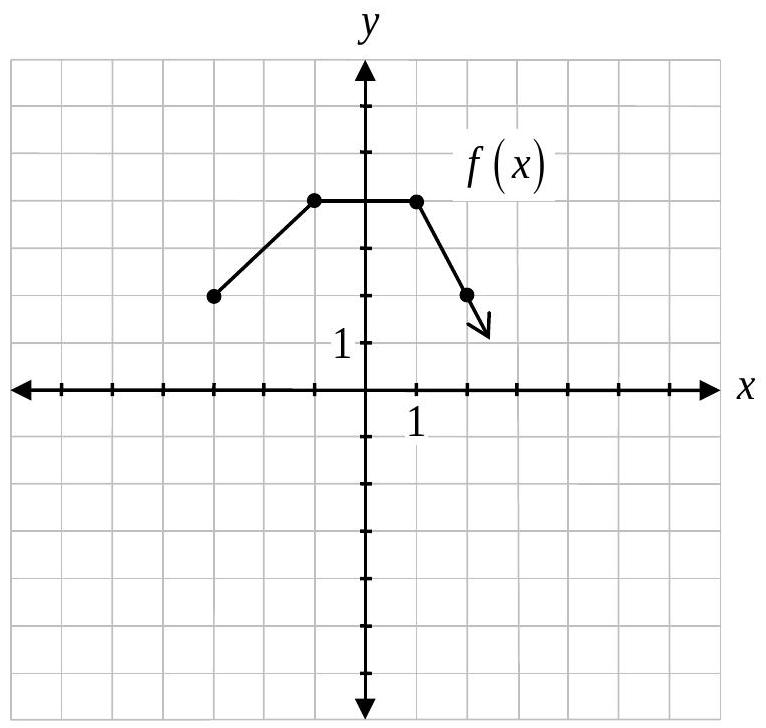
\includegraphics[max width=\textwidth, alt={}, center]{f67fedaf-ea11-42ad-a16e-f30d2fcf2bd3-220_728_766_489_670}

\section*{Solution}
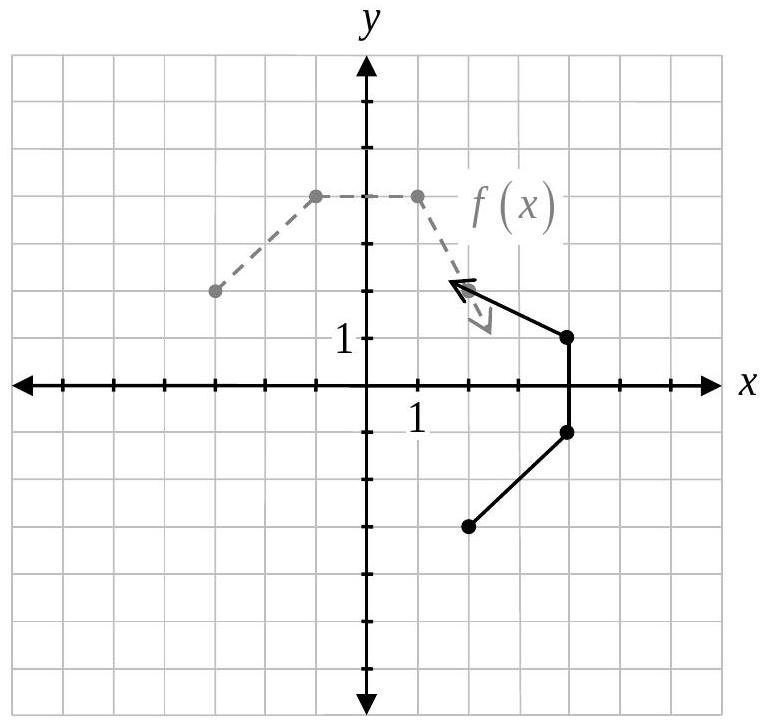
\includegraphics[max width=\textwidth, alt={}, center]{f67fedaf-ea11-42ad-a16e-f30d2fcf2bd3-220_725_768_1323_249}\\
□\\
1 mark

Prove the following identity for all permissible values of $\theta$.

$$
\frac{1+\cos \theta}{1-\sin ^{2} \theta}=\sec \theta+\tan ^{2} \theta+1
$$

\section*{Solution}
\section*{Method 1}
\begin{center}
\begin{tabular}{|l|l|l|}
\hline
Left-Hand Side & Right-Hand Side & \multirow{2}{*}{} \\
\hline
$\frac{1+\cos \theta}{1-\sin ^{2} \theta}$ & $\sec \theta+\tan ^{2} \theta+1$ &  \\
\hline
$\frac{1+\cos \theta}{\cos ^{2} \theta}$ &  & 1 mark for algebraic strategies \\
\hline
$\frac{1}{\cos ^{2} \theta}+\frac{1}{\cos \theta}$ &  & 1 mark for logical process to prove the identity \\
\hline
$\sec ^{2} \theta+\sec \theta$ &  & 1 mark for correct substitution of appropriate identities \\
\hline
$\tan ^{2} \theta+1+\sec \theta$ &  & 3 marks \\
\hline
\end{tabular}
\end{center}

\section*{Solution}
\section*{Method 2}
\begin{center}
\begin{tabular}{|l|l|l|}
\hline
Left-Hand Side & Right-Hand Side & \multirow{2}{*}{1 mark for algebraic strategies} \\
\hline
$\frac{1+\cos \theta}{\cos ^{2} \theta}$ & \( \begin{aligned} & \frac{1}{\cos \theta}+\sec ^{2} \theta \\ & \frac{1}{\cos \theta}+\frac{1}{\cos ^{2} \theta} \end{aligned} \) &  \\
\hline
 & $\frac{\cos \theta+1}{\cos ^{2} \theta}$ & \begin{tabular}{l}
1 mark for correct substitution of appropriate identities \\
3 marks \\
\end{tabular} \\
\hline
 &  &  \\
\hline
\end{tabular}
\end{center}

Thomas used graphs to solve the equation $e^{x+2}=\sqrt{-(x+1)}$.\\
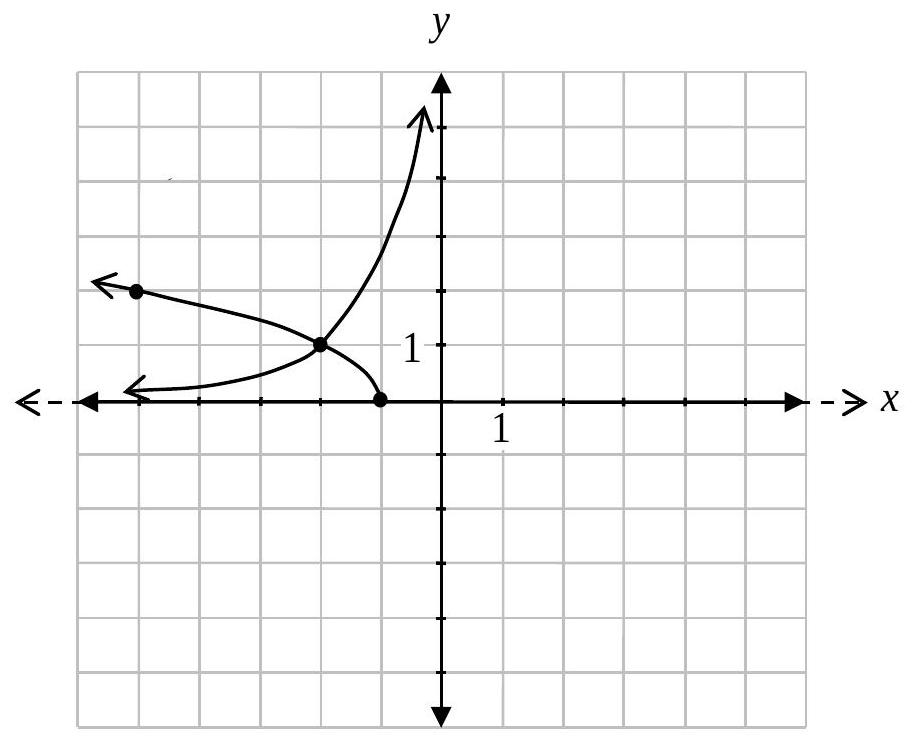
\includegraphics[max width=\textwidth, alt={}, center]{f67fedaf-ea11-42ad-a16e-f30d2fcf2bd3-223_744_914_483_623}

He incorrectly states the solution as $(-2,1)$.\\
Describe how Thomas should have stated the solution.

\section*{Solution}
He stated his solution as a coordinate point; his solution should have only been the value of $x$.

Given the graph of $y=f(x)$, sketch the graph of $y=\sqrt{f(x)}$.\\
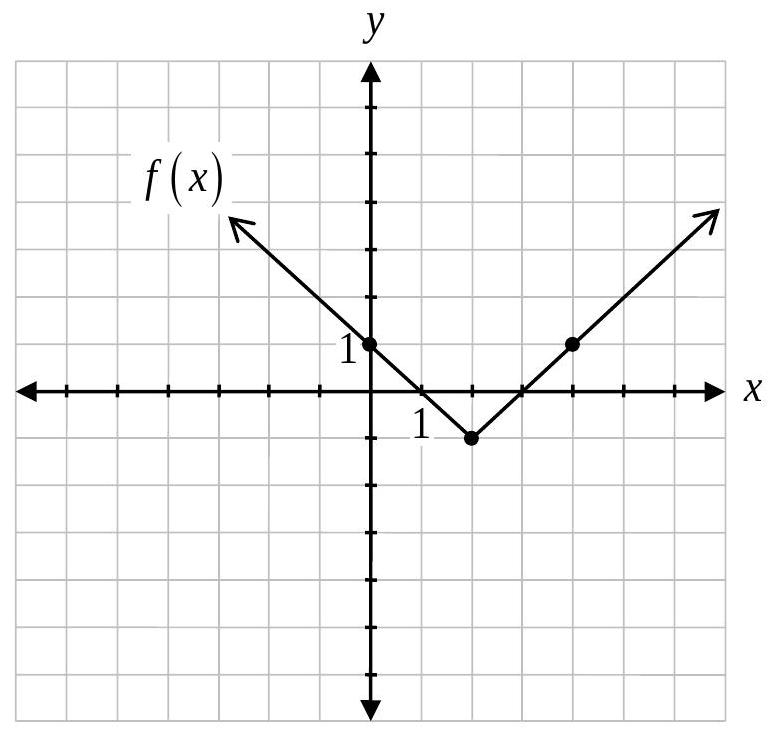
\includegraphics[max width=\textwidth, alt={}, center]{f67fedaf-ea11-42ad-a16e-f30d2fcf2bd3-224_736_779_481_689}

\section*{Solution}
\begin{center}
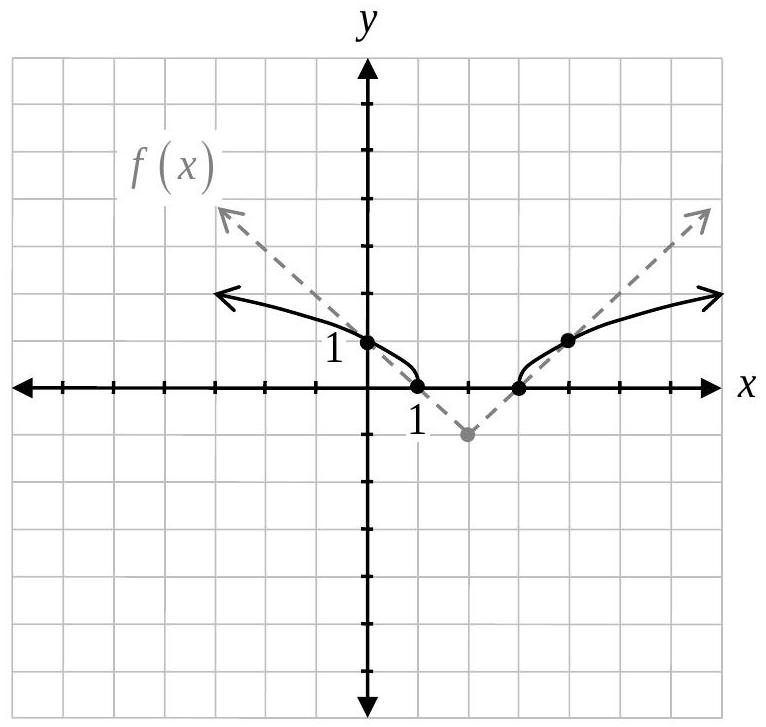
\includegraphics[max width=\textwidth, alt={}]{f67fedaf-ea11-42ad-a16e-f30d2fcf2bd3-224_727_766_1332_244}
\end{center}

1 mark for restricting domain\\
$\frac{1}{2}$ mark for shape between both pairs of invariant points\\
$\frac{1}{2}$ mark for shape above both pairs of invariant points

2 marks

When a polynomial, $P(x)$, is divided by ( $x-2$ ) the resulting equation is\\
$\frac{P(x)}{x-2}=x^{2}-x+1+\frac{3}{x-2}$.\\
a) Explain why $x-2$ is not a factor of $P(x)$.\\
b) Determine the equation for the polynomial function $P(x)$.

\section*{Solution}
a) There is a remainder when $P(x)$ is divided by $x-2$.\\
b) $P(x)=(x-2)\left(x^{2}-x+1\right)+3$\\
or\\
$P(x)=x^{3}-3 x^{2}+3 x+1$

Determine the equation for $g(x)$ in terms of $f(x)$.\\
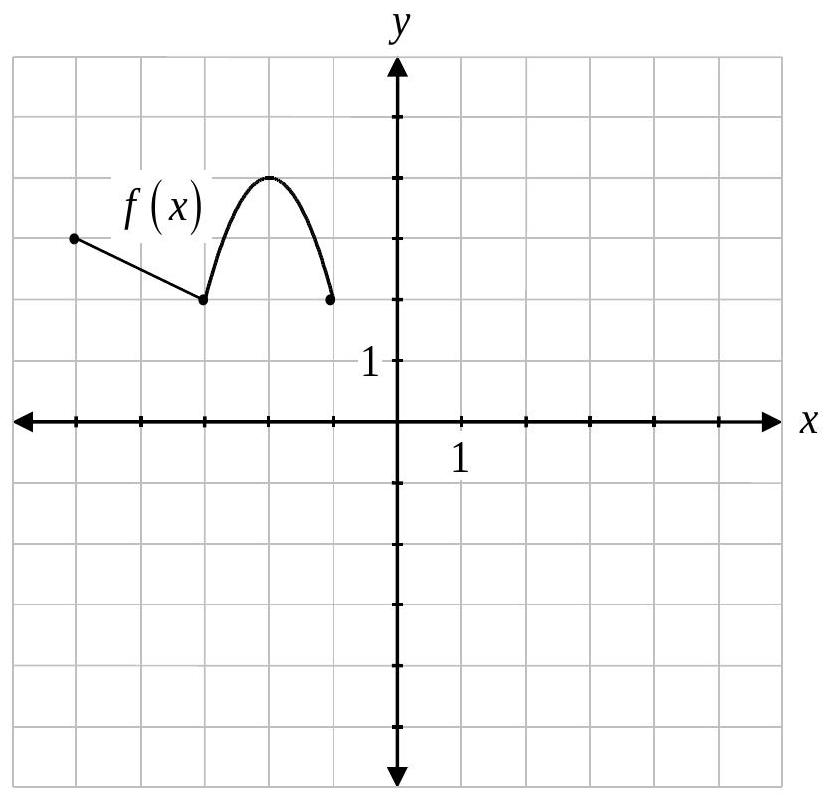
\includegraphics[max width=\textwidth, alt={}, center]{f67fedaf-ea11-42ad-a16e-f30d2fcf2bd3-226_798_830_470_249}\\
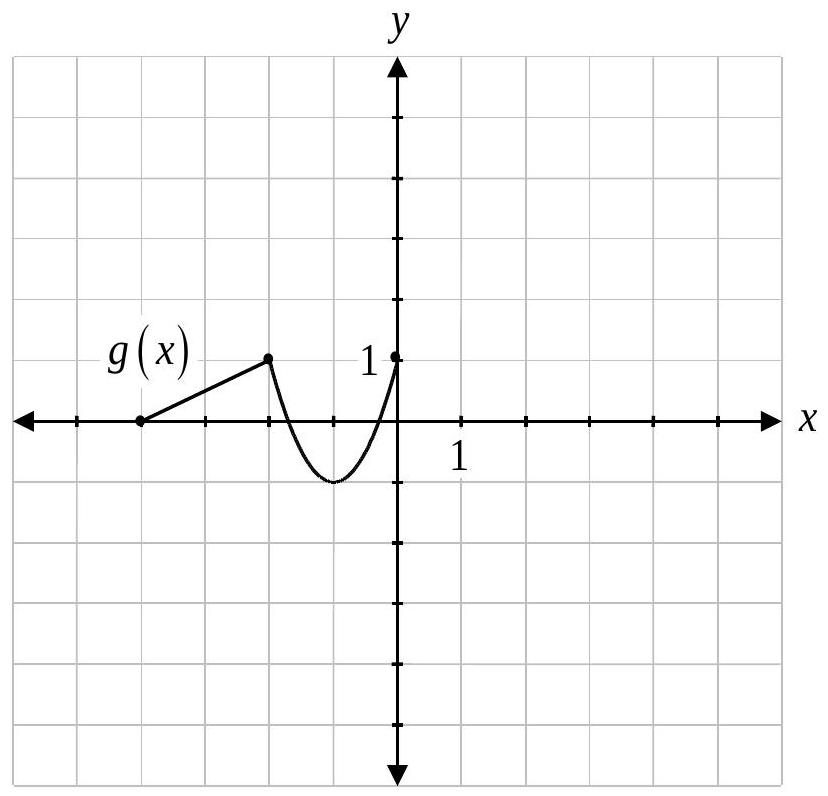
\includegraphics[max width=\textwidth, alt={}, center]{f67fedaf-ea11-42ad-a16e-f30d2fcf2bd3-226_796_828_470_1110}

\section*{Solution}
$g(x)=-f(x-1)+3$\\
1 mark for vertical reflection\\
1 mark for horizontal translation\\
1 mark for vertical translation

3 marks

Explain why the binomial expansion of $(2 x+y)^{9}$ does not have a middle term.

\section*{Solution}
The expansion contains $n+1$ terms. Since $n$ equals 9 , there are 10 terms, which would not allow for a middle term.

Using the laws of logarithms, completely expand the expression $\log \left(\frac{5 \sqrt{a}}{b^{3}}\right)$.

\section*{Solution}
$$
\begin{array}{ll}
\log 5+\frac{1}{2} \log a-3 \log b & 1 \text { mark for product law } \\
& 1 \text { mark for power law ( } 1 / 2 \text { mark for each) } \\
& 1 \text { mark for quotient law }
\end{array}
$$

3 marks

Identify $10^{\circ}$ in radians.\\
a) $\frac{1800}{\pi}$\\
b) $\frac{\pi}{1800}$\\
c) $\frac{18}{\pi}$\\
d) $\frac{\pi}{18}$

\section*{Question 17}
The polynomial function, $P(x)=a(x-1)^{2}(x+4)^{2}$, has a $y$-intercept of -8 .\\
Identify the value of $a$.\\
a) -2\\
b) $-\frac{1}{2}$\\
c) $\frac{1}{2}$\\
d) 2

Identify the value of $\log _{4}\left(\frac{1}{16}\right)$.\\
a) -2\\
b) $-\frac{1}{2}$\\
c) $\frac{1}{2}$\\
d) 2

Question 19

Given the angle $\frac{25 \pi}{7}$, identify the coterminal angle on the interval $[-2 \pi, 0]$.\\
a) $\frac{18 \pi}{7}$\\
b) $\frac{11 \pi}{7}$\\
с) $-\frac{3 \pi}{7}$\\
d) $-\frac{10 \pi}{7}$

Question 20

Identify which expression cannot be evaluated.\\
a) ${ }_{7} P_{0}$\\
b) ${ }_{7} P_{6}$\\
c) ${ }_{7} P_{7}$\\
d) ${ }_{7} P_{8}$

Identify the graph of $f(x)=\frac{-3 x}{2 x+4}$.\\
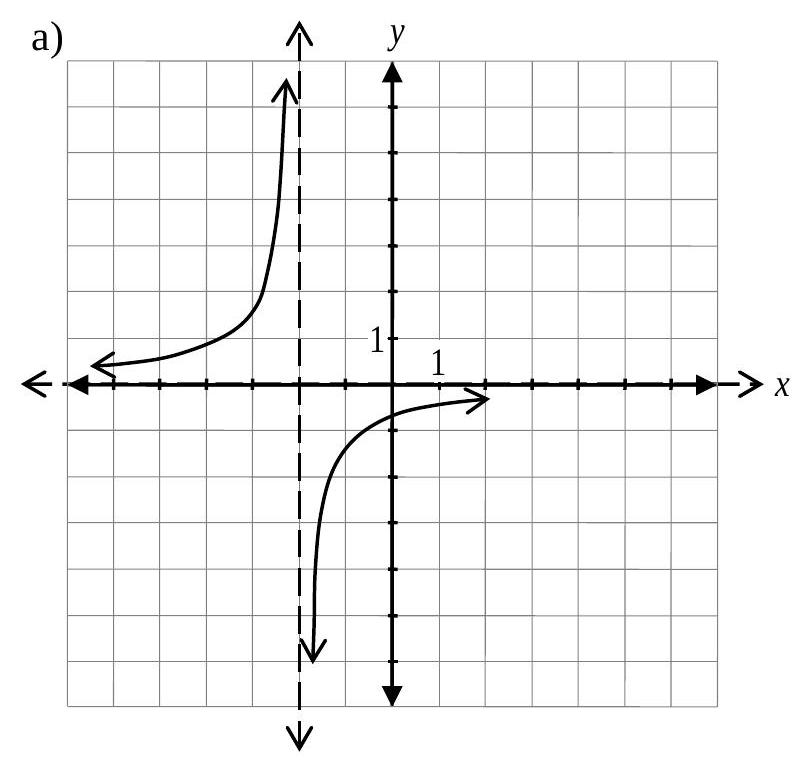
\includegraphics[max width=\textwidth, alt={}, center]{f67fedaf-ea11-42ad-a16e-f30d2fcf2bd3-231_766_809_588_216}\\
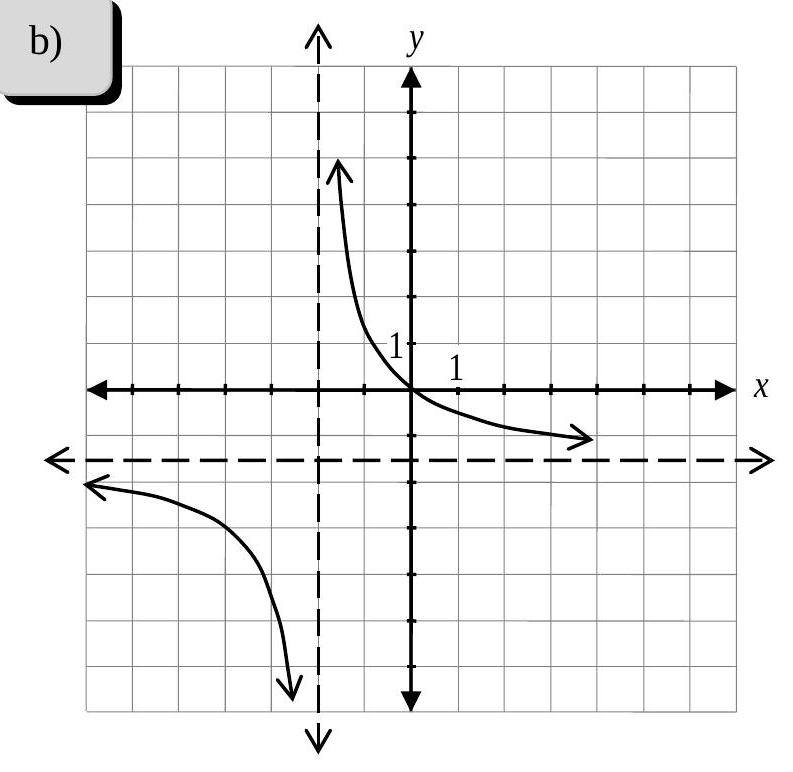
\includegraphics[max width=\textwidth, alt={}, center]{f67fedaf-ea11-42ad-a16e-f30d2fcf2bd3-231_772_793_584_1093}\\
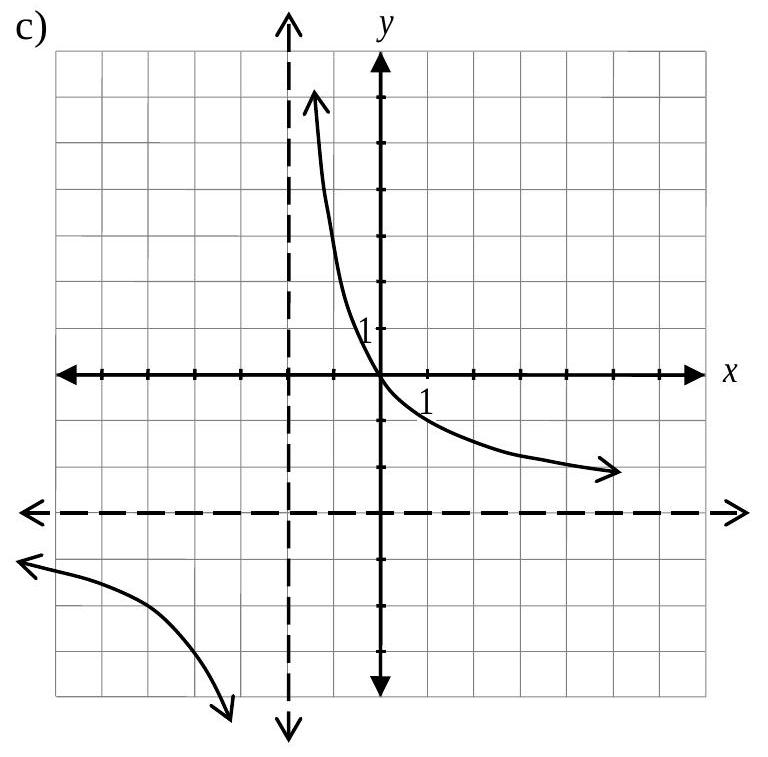
\includegraphics[max width=\textwidth, alt={}, center]{f67fedaf-ea11-42ad-a16e-f30d2fcf2bd3-231_757_768_1405_232}\\
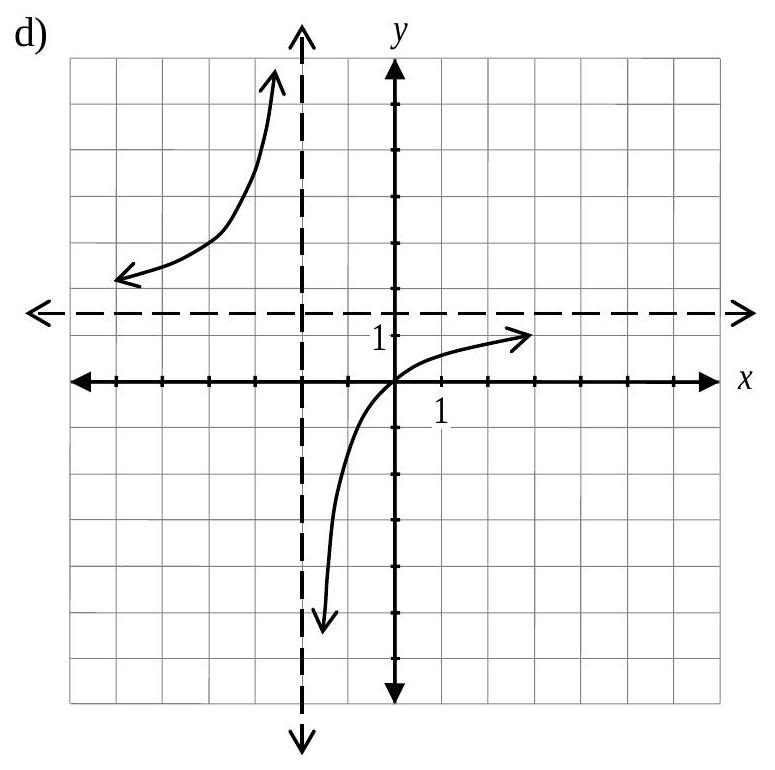
\includegraphics[max width=\textwidth, alt={}, center]{f67fedaf-ea11-42ad-a16e-f30d2fcf2bd3-231_770_775_1398_1108}

Given a point $(-2,0)$ on the graph of $y=f(x)$, identify the coordinates of the corresponding point on the graph of $y=4 f\left(\frac{1}{2} x\right)$.\\
a) $(-8,0)$\\
b) $(-4,0)$\\
c) $(-2,0)$\\
d) $(-1,0)$

Question 23

Identify the non-permissible value of $\theta$ for the expression $\frac{\cos \theta}{1+\sin \theta}$.\\
a) $\frac{\pi}{2}$\\
b) $\pi$\\
c) $\frac{3 \pi}{2}$\\
d) $2 \pi$

Question 24

Identify the function with an asymptote at $x=-3$.\\
a) $y=\log (x+3)$\\
b) $y=\log x+3$\\
c) $y=\log (x-3)$\\
d) $y=\log x-3$

Evaluate the following expression.

$$
\tan \left(\frac{2 \pi}{3}\right) \csc \left(\frac{-2 \pi}{3}\right)+\cos (3 \pi)
$$

\section*{Solution}
$\begin{array}{cl}(-\sqrt{3})\left(-\frac{2}{\sqrt{3}}\right)+(-1) & 1 \text { mark for } \tan \left(\frac{2 \pi}{3}\right)(1 / 2 \text { mark for quadrant, } 1 / 2 \text { mark for value }) \\ 2-1 & 1 \text { mark for } \csc \left(-\frac{2 \pi}{3}\right)(1 / 2 \text { mark for quadrant, } 1 / 2 \text { mark for value })\end{array}$ 1 mark for $\cos (3 \pi)$

3 marks

State the range of the graph below.\\
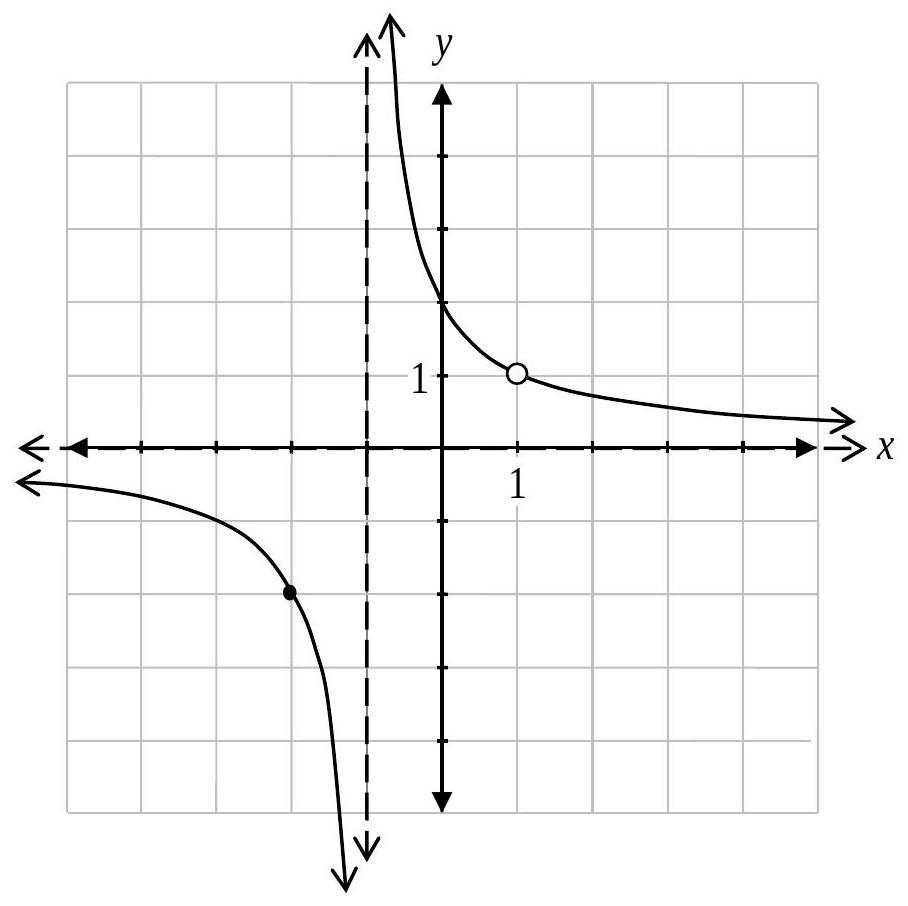
\includegraphics[max width=\textwidth, alt={}, center]{f67fedaf-ea11-42ad-a16e-f30d2fcf2bd3-234_906_908_442_620}

\section*{Solution}
Range: □ $\{y \in \mathbb{R}, y \neq 0$ and $y \neq 1\}$ 1 mark ( $\frac{1}{2}$ mark for $y \neq 0, \frac{1}{2}$ mark for $y \neq 1$ ) 1 mark

Sketch the graph of the function $f(x)=\frac{2 x^{2}-5 x}{x}$.

\section*{Solution}
\begin{center}
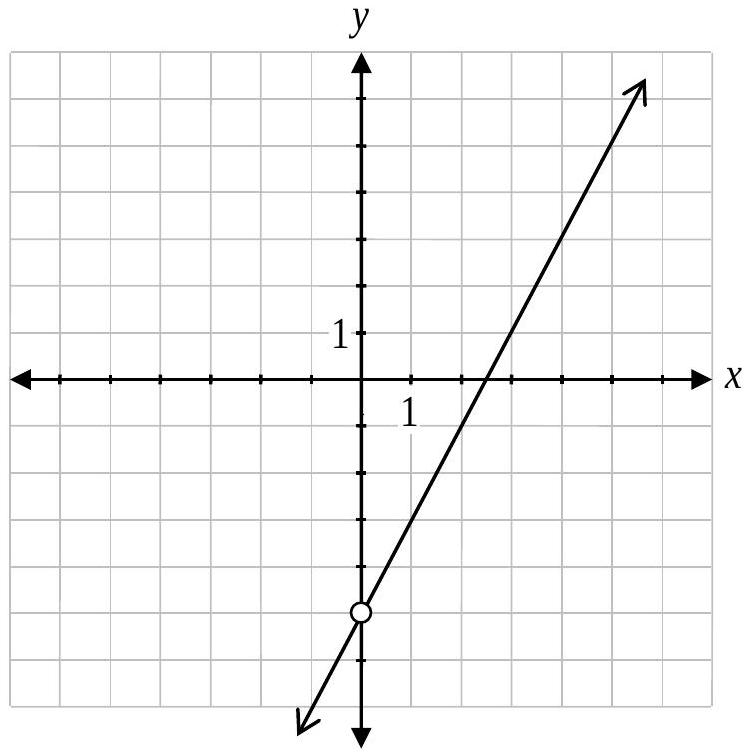
\includegraphics[max width=\textwidth, alt={}]{f67fedaf-ea11-42ad-a16e-f30d2fcf2bd3-235_755_755_601_249}
\end{center}

1 mark for point of discontinuity (hole) at $(0,-5) \left(\frac{1}{2}\right.$ mark for $x=0,1 / 2$ mark for $\left.y=-5\right)$ 1 mark for shape of a linear function

2 marks

State a possible value of $n$ if the polynomial function $P(x)=(x-1)^{2}(x+2)^{n}$ has a range of $[0, \infty)$.

\section*{Solution}
$n=2$

Note(s):

\begin{itemize}
  \item Accept any even positive value of $n$, including zero.
\end{itemize}

Sketch the graph of $y=\left(\frac{1}{2}\right)^{x-1}$.

\section*{Solution}
\begin{center}
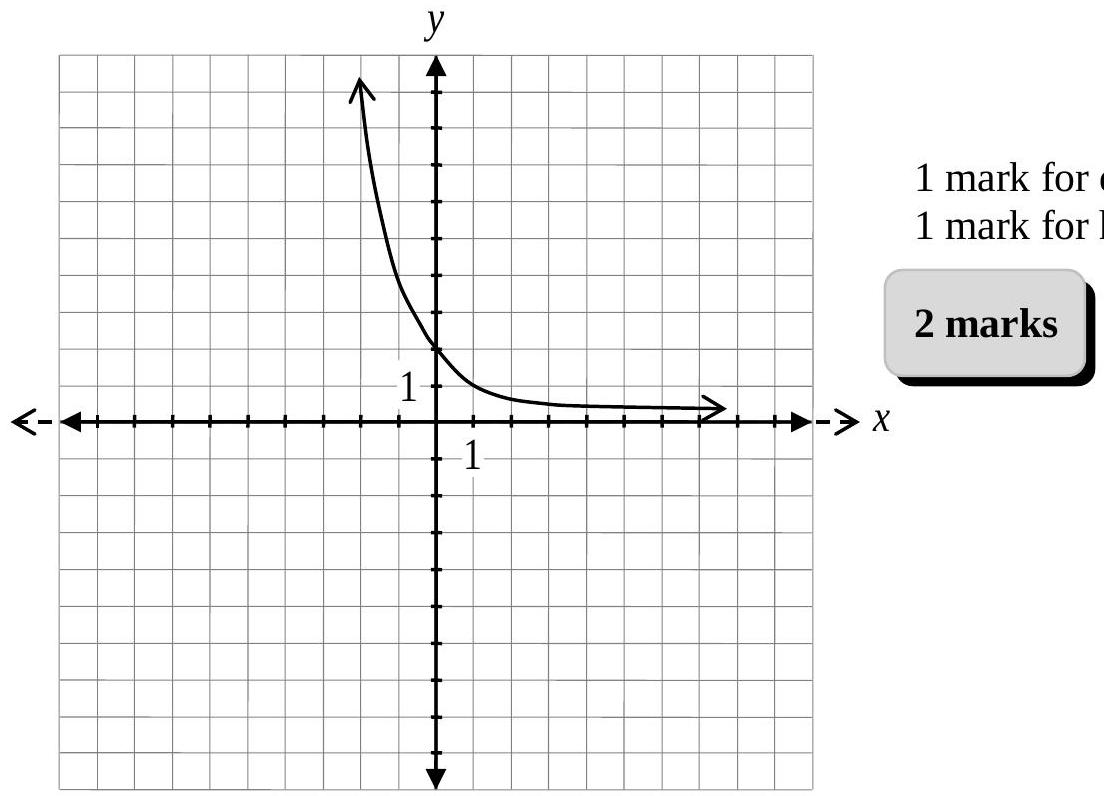
\includegraphics[max width=\textwidth, alt={}]{f67fedaf-ea11-42ad-a16e-f30d2fcf2bd3-237_796_1104_595_201}
\end{center}

Solve.

$$
\log _{x} 27=3
$$

\section*{Solution}
$$
\begin{aligned}
x^{3} & =27 & & 1 \text { mark for exponential form } \\
x & =3 & & \mathbf{1} \text { mark }
\end{aligned}
$$

Sketch at least two periods of the graph $y=\tan x$.

\section*{Solution}
\begin{center}
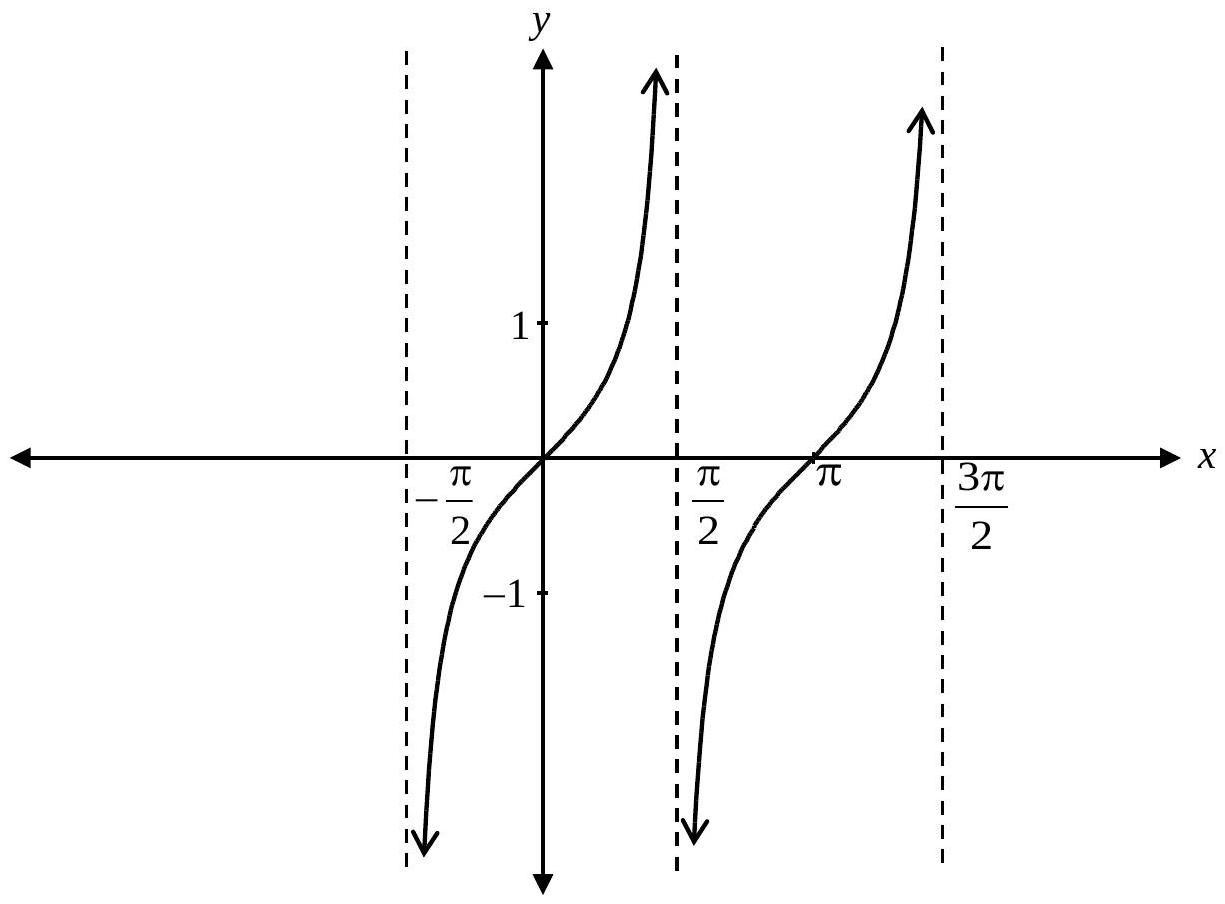
\includegraphics[max width=\textwidth, alt={}]{f67fedaf-ea11-42ad-a16e-f30d2fcf2bd3-239_904_1225_577_249}
\end{center}

1 mark for increasing trigonometric function\\
1 mark for asymptotic behaviour approaching $x=\frac{\pi}{2}+k \pi, k \in \mathbb{Z}$\\
2 marks

Given the graph of $f(x)$, state the domain of $\frac{1}{f(x)}$.\\
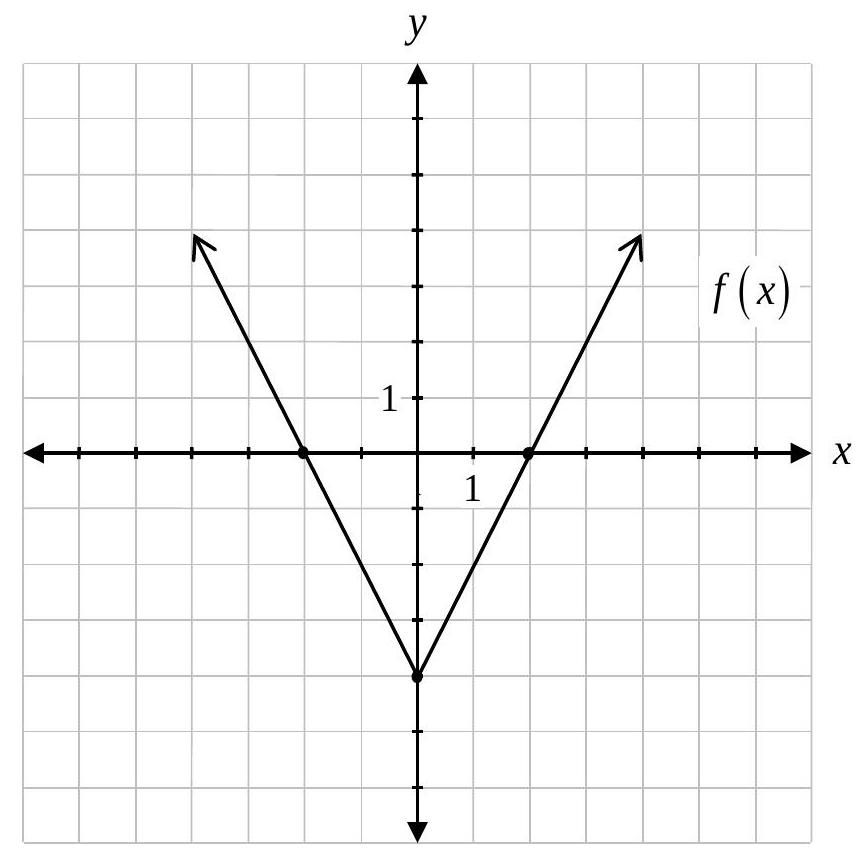
\includegraphics[max width=\textwidth, alt={}, center]{f67fedaf-ea11-42ad-a16e-f30d2fcf2bd3-240_856_865_500_644}

\section*{Solution}
Domain: $\{$ $\_\_\_\_$ $\{x \in \mathbb{R}, x \neq \pm 2\}$

1 mark ( $\frac{1}{2}$ mark for $x \neq 2,1 / 2$ mark for $x \neq-2$ )\\
1 mark

Determine the values of $\mathrm{A}, \mathrm{B}$, and D of the sinusoidal function in the form $y=\mathrm{A} \sin (\mathrm{B} x)+\mathrm{D}$.\\
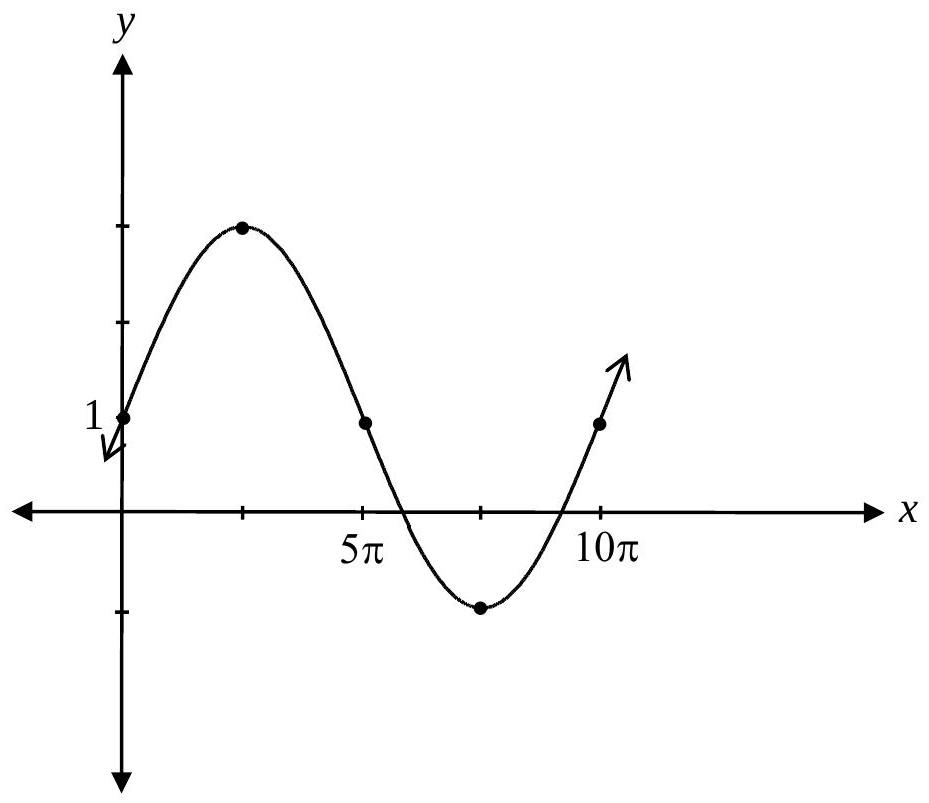
\includegraphics[max width=\textwidth, alt={}, center]{f67fedaf-ea11-42ad-a16e-f30d2fcf2bd3-241_803_929_472_691}

\section*{Solution}
$\mathrm{A}=$ $\_\_\_\_$ 2

1 mark for A\\
$\mathrm{B}=$ $\_\_\_\_$ $\frac{1}{5}$

1 mark for B

D = $\_\_\_\_$ 1

1 mark for D\\
3 marks

Determine if the point $\left(-\frac{\sqrt{7}}{5}, \frac{2}{5}\right)$ is on the unit circle.\\
Justify your answer.

\section*{Solution}
$$
\begin{aligned}
x^{2}+y^{2} & =1 \\
\text { Left-hand side } & =\left(-\frac{\sqrt{7}}{5}\right)^{2}+\left(\frac{2}{5}\right)^{2} \\
& =\frac{7}{25}+\frac{4}{25} \\
& =\frac{11}{25} \\
\frac{11}{25} & \neq 1 \\
& \therefore \text { not on the unit circle }
\end{aligned}
$$

Solve, algebraically.

$$
\frac{{ }_{n} C_{5}}{{ }_{n} C_{4}}=6
$$

\section*{Solution}
$\frac{n!}{\frac{(n-5)!5!}{n!}}=6$\\
$\frac{(n-4)!4!}{n!(n-4)!4!}=6$\\
$\frac{n!(n-5)!5!}{}$\\
$\frac{n!(n-4)(n-5)!4!}{n!(n-5)!5 \cdot 4!}=6$\\
$\frac{n-4}{5}=6$\\
$n-4=30$\\
$n=34$\\
$\frac{1}{2}$ mark for substitution into equation

1 mark for factorial expansion\\
( $\frac{1}{2}$ mark for numerical factors; $\frac{1}{2}$ mark for factors with variables) 1 mark for simplification of factorials\\
( $\frac{1}{2}$ mark for numerical factors; $\frac{1}{2}$ mark for factors with variables)

Given $\sin \alpha=\frac{4}{5}$, where $\alpha$ is in quadrant II, determine the exact value of $\sin 2 \alpha$.

\section*{Solution}
\begin{center}
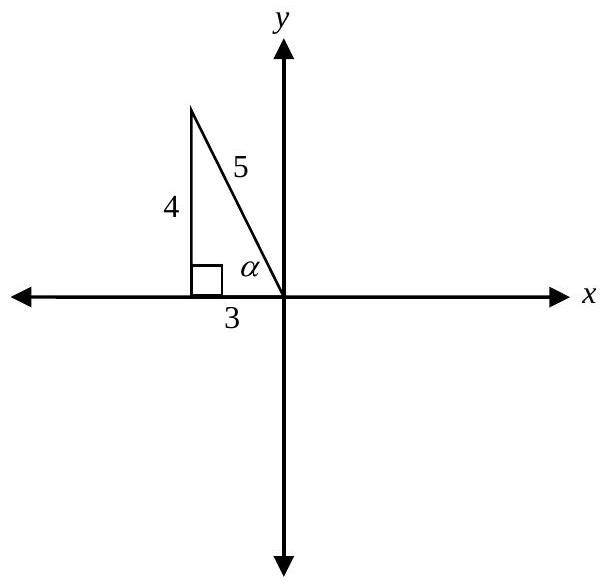
\includegraphics[max width=\textwidth, alt={}]{f67fedaf-ea11-42ad-a16e-f30d2fcf2bd3-244_586_607_603_328}
\end{center}

$$
\begin{aligned}
x^{2}+y^{2} & =r^{2} \\
x^{2}+16 & =25 \\
x^{2} & =9 \\
x & = \pm 3 \\
x & =-3
\end{aligned}
$$

$\cos \alpha=-\frac{3}{5}$\\
$\sin 2 \alpha=2 \sin \alpha \cos \alpha$

$$
\begin{aligned}
& =2\left(\frac{4}{5}\right)\left(-\frac{3}{5}\right) \\
& =-\frac{24}{25}
\end{aligned}
$$

$\frac{1}{2}$ mark for value of $x$\\
$\frac{1}{2}$ mark for $\cos \alpha$

1 mark for substitution into correct identity\\
2 marks

Note(s):

\begin{itemize}
  \item Accept any of the following values for $x: x= \pm 3 ; x=-3$; or $x=3$.
\end{itemize}

Given the functions $f(x)=x+1$ and $g(x)=\sqrt{x}$,\\
a) determine the equation of $g(f(x))$.\\
b) sketch the graph of $g(f(x))$.

\section*{Solution}
a) $g(f(x))=\sqrt{x+1}$\\
b)\\
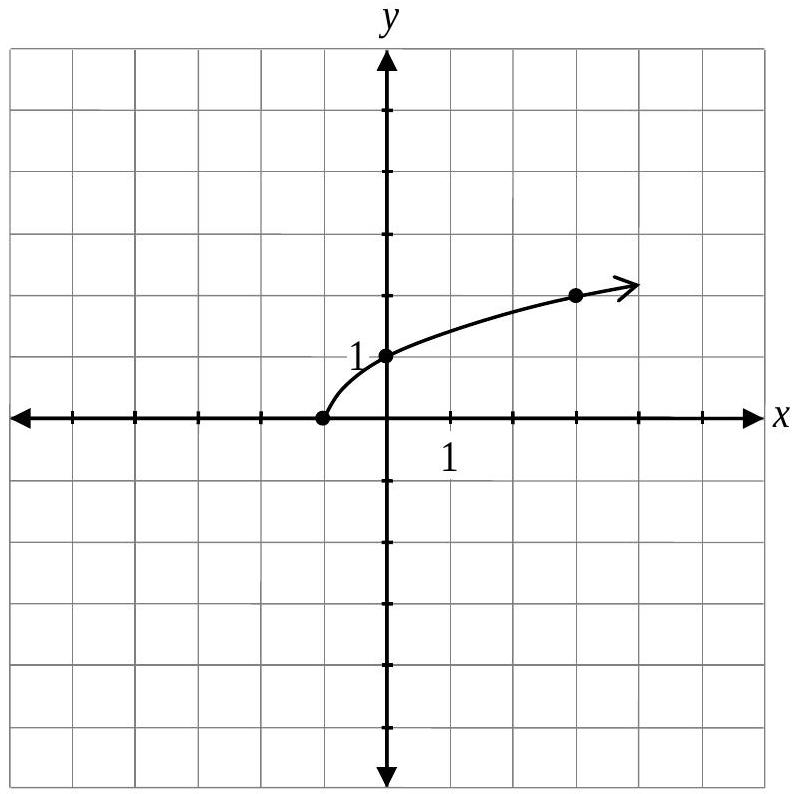
\includegraphics[max width=\textwidth, alt={}, center]{f67fedaf-ea11-42ad-a16e-f30d2fcf2bd3-245_794_798_990_249}

\section*{1 mark}
1 mark for domain of $g(f(x))$\\
1 mark for shape consistent with $g(f(x))$\\
2 marks

Steve is asked to determine an equation with a larger period than the period of the graph of $y=\cos (2 x)$.

Justify why Steve's answer of $y=\cos (6 x)$ is incorrect.

\section*{Solution}
Steve's equation needs to have a value of $|b|$ less than $2 . \quad 1$ mark\\
or\\
Steve's graph would have a period of $\frac{2 \pi}{6}=\frac{\pi}{3}$, which is smaller than $\frac{2 \pi}{2}=\pi$, the period of the given graph.

Given the graphs of $f(x)$ and $g(x)$,\\
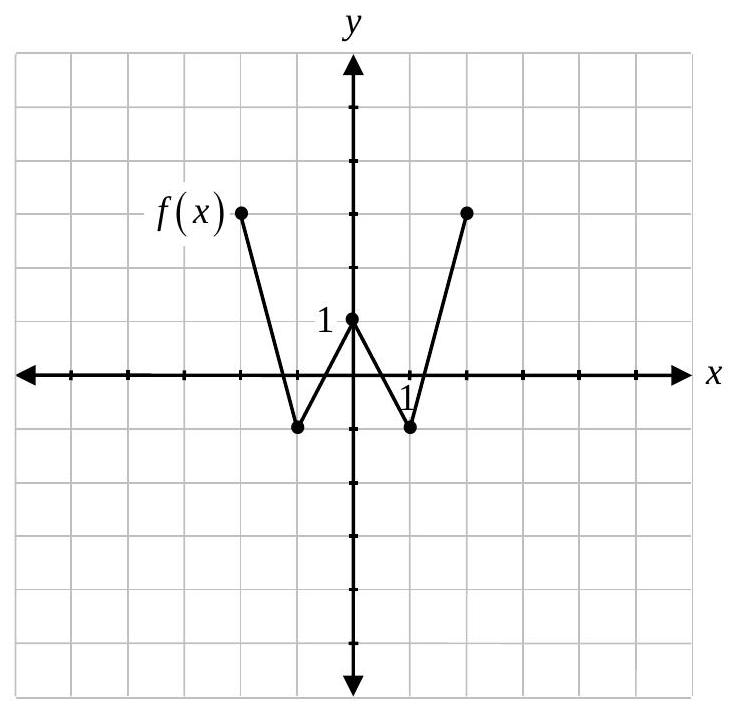
\includegraphics[max width=\textwidth, alt={}, center]{f67fedaf-ea11-42ad-a16e-f30d2fcf2bd3-247_712_736_459_311}\\
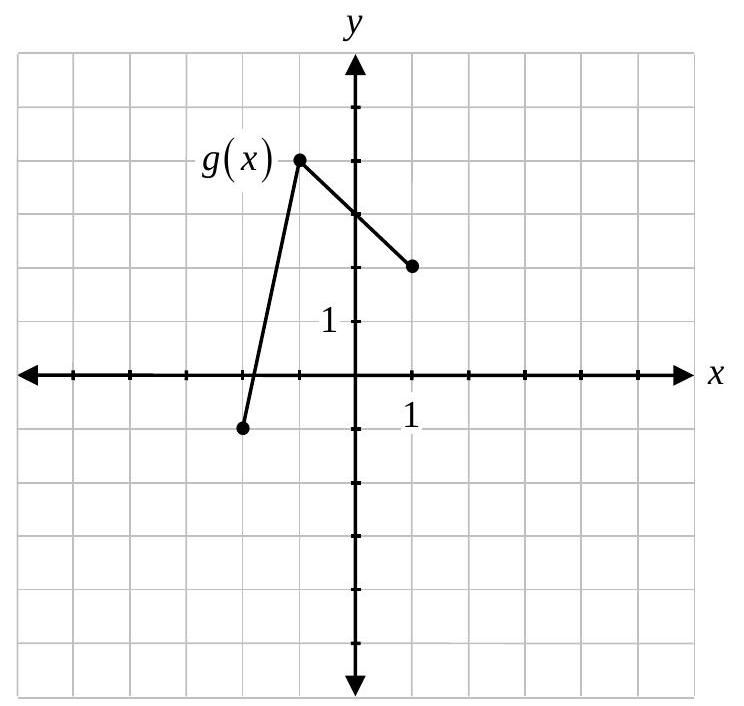
\includegraphics[max width=\textwidth, alt={}, center]{f67fedaf-ea11-42ad-a16e-f30d2fcf2bd3-247_706_744_459_1136}\\
a) determine the value of $(f \cdot g)(-1)$.\\
b) determine the value of $g(f(0))$.

\section*{Solution}
a) $(f \cdot g)(-1)=(-1)(4) \quad 1$ mark for value of $(f \cdot g)(-1)$

$$
=-4
$$

b) $f(0)=1$\\
$\frac{1}{2}$ mark for $f(0)$\\
$g(f(0))=2$\\
$\frac{1}{2}$ mark for $g(f(0))$ consistent with $f(0)$ value\\
1 mark

Sketch the graph of $P(x)=-(x-1)^{3}(x-3)(x+1)$.

\section*{Solution}
\begin{center}
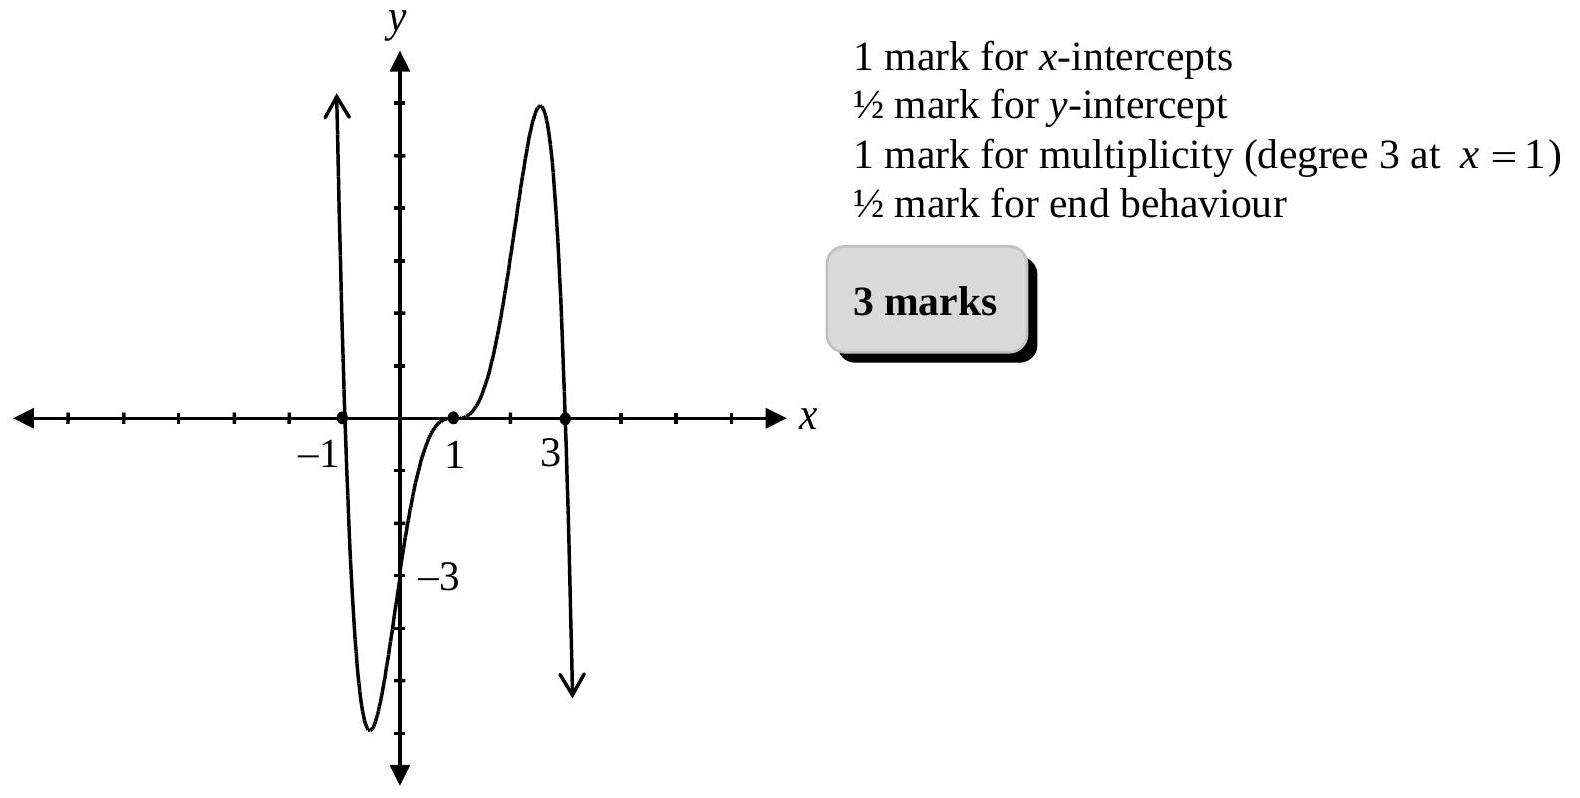
\includegraphics[max width=\textwidth, alt={}]{f67fedaf-ea11-42ad-a16e-f30d2fcf2bd3-248_798_1580_567_298}
\end{center}

The point $(-\sqrt{3}, 1)$ is on the terminal arm of an angle $\theta$, in standard position.\\
a) Determine $\tan \theta$.\\
b) Determine a possible value of $\theta$, in radians.

\section*{Solution}
a) $\tan \theta=-\frac{1}{\sqrt{3}}$ 1 mark\\
b) $\theta=\frac{5 \pi}{6}$

Describe the transformation used to obtain the graph of $y=\log _{5} x$ given the graph of $y=5^{x}$.

\section*{Solution}
The graph of $y=\log _{5} x$ is obtained by reflecting the graph of $y=5^{x}$ over the line $y=x$.\\
or

The graph of $y=\log _{5} x$ is the inverse of $y=5^{x}$.

Solve $\sin \theta=-\frac{\sqrt{3}}{2}$, where $\theta \in \mathbb{R}$.

\section*{Solution}
$\theta=\frac{4 \pi}{3}, \frac{5 \pi}{3}$\\
1 mark for values of $\theta$ ( $\frac{1}{2}$ mark for each value)\\
$\theta=\left\{\begin{array}{l}\frac{4 \pi}{3}+2 k \pi, k \in \mathbb{Z} \\ \frac{5 \pi}{3}+2 k \pi, k \in \mathbb{Z}\end{array}\right\}$

1 mark for general solution\\
2 marks\\
or\\
$\theta=240^{\circ}, 300^{\circ}$\\
$\theta=\left\{\begin{array}{l}240^{\circ}+360^{\circ} k, k \in \mathbb{Z} \\ 300^{\circ}+360^{\circ} k, k \in \mathbb{Z}\end{array}\right\}$

Given that the point $(a, b)$ is on the graph of $f(x)$, describe how you would determine the corresponding point on the graph of $y=\sqrt{f(x)}$.

\section*{Solution}
The value of $a$ stays the same, square root the value of $b$.

Evaluate.

$$
\cos \left(\frac{\pi}{20}\right) \cos \left(\frac{\pi}{5}\right)-\sin \left(\frac{\pi}{20}\right) \sin \left(\frac{\pi}{5}\right)
$$

\section*{Solution}
$\cos \left(\frac{\pi}{20}+\frac{\pi}{5}\right)$\\
$\frac{1}{2}$ mark for substitution of an appropriate identity\\
$\cos \left(\frac{\pi}{20}+\frac{4 \pi}{20}\right)$\\
$\cos \left(\frac{5 \pi}{20}\right)$\\
$\cos \left(\frac{\pi}{4}\right)$\\
$\frac{\sqrt{2}}{2}$\\
$\frac{1}{2}$ mark for exact value\\
1 mark

Describe the transformations used to obtain the graph of the function $y=f(-x+6)-8$ from the graph of $y=f(x)$.

\section*{Solution}
Reflect the graph of $y=f(x)$ over the $y$-axis and then translate 6 units right and 8 units down.

\begin{displayquote}
1 mark for horizontal reflection\\
1 mark for horizontal translation\\
1 mark for vertical translation
\end{displayquote}

3 marks

Note(s):

\begin{itemize}
  \item Deduct 1 mark if correct transformations are given in the wrong order.
\end{itemize}

State the equations of all the asymptotes of the function, $y=\frac{1}{3 x+1}$.

\section*{Solution}
$y=0$\\
$x=-\frac{1}{3}$

1 mark for horizontal asymptote

1 mark for vertical asymptote\\
2 marks

Determine the zeros of the polynomial function $P(x)=2 x^{3}+5 x^{2}-4 x-3$.

\section*{Solution}
$P(1)=2(1)^{3}+5(1)^{2}-4(1)-3 \quad 1$ mark for identifying one possible value of $x$\\
$P(1)=0$\\
$(x-1)$ is a factor

\begin{center}
\begin{tabular}{c|cccc}
1 & 2 & 5 & -4 & -3 \\
 & $\downarrow$ & 2 & 7 & 3 \\
\hline
 & 2 & 7 & 3 & 0 \\
\hline
\end{tabular}
\end{center}

1 mark for synthetic division (or for any equivalent strategy)\\
$P(x)=(x-1)\left(2 x^{2}+7 x+3\right)$\\
$\frac{1}{2}$ mark for consistent factors\\
$0=(x-1)(2 x+1)(x+3)$\\
$x=1 \quad x=-\frac{1}{2} \quad x=-3$\\
$\frac{1}{2}$ mark for all zeros\\
3 marks

Determine the equation of the radical function represented by the graph.\\
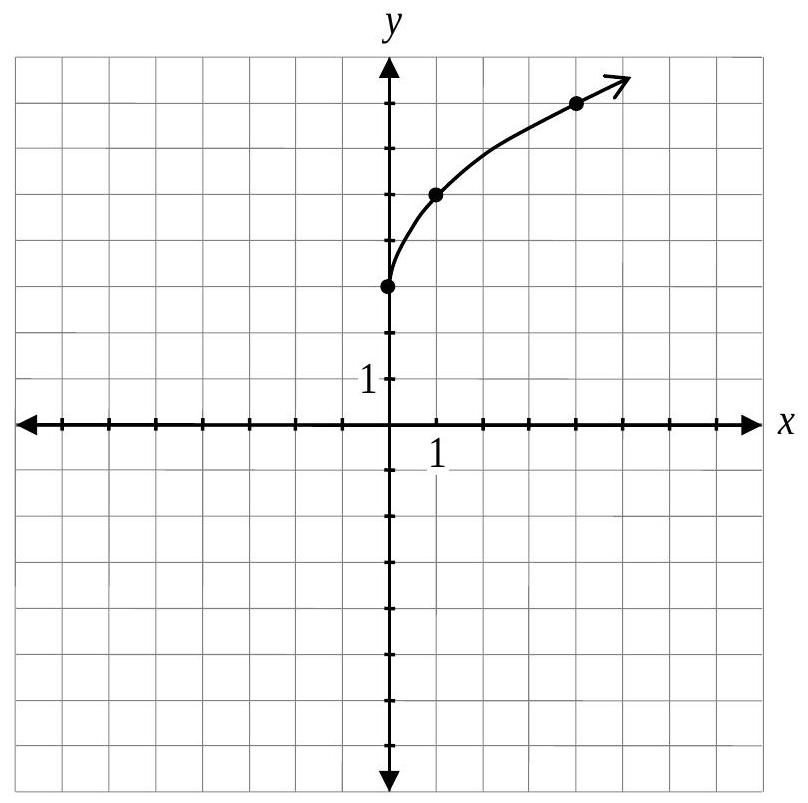
\includegraphics[max width=\textwidth, alt={}, center]{f67fedaf-ea11-42ad-a16e-f30d2fcf2bd3-257_803_808_532_681}

\section*{Solution}
$y=2 \sqrt{x}+3$\\
1 mark for vertical stretch\\
1 mark for vertical translation\\
or\\
$y=\sqrt{4 x}+3$

1 mark for horizontal stretch\\
1 mark for vertical translation

2 marks

Determine the length of the radius, $r$, given an arc length of 20 metres and a central angle of $160^{\circ}$.\\
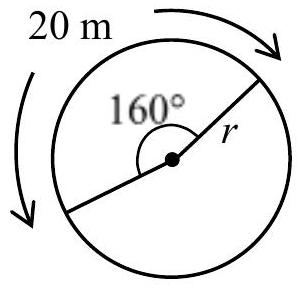
\includegraphics[max width=\textwidth, alt={}, center]{f67fedaf-ea11-42ad-a16e-f30d2fcf2bd3-258_289_303_515_782}

\section*{Solution}
$$
\begin{aligned}
\theta & =(160)\left(\frac{\pi}{180}\right) \\
& =\frac{8 \pi}{9} \\
r & =\frac{s}{\theta} \\
r & =\frac{20}{\left(\frac{8 \pi}{9}\right)} \\
r & =\frac{180}{8 \pi} \mathrm{~m} \\
\text { or } & 1 \text { mark for conversion } \\
r & =7.162 \mathrm{~m}
\end{aligned}
$$

There are eight cars parked in a row. Determine the number of possible arrangements of these eight cars if Mrs. Jones must always park in the third spot and Mr. Rodriguez must always park in the last spot.

\section*{Solution}
$\underline{6} \cdot \underline{5} \cdot \underline{1} \cdot \underline{4} \cdot \underline{3} \cdot \underline{2} \cdot \underline{1} \cdot \underline{1}$

720

Bill wins $\$ 1300000$ in a lottery and invests the entire amount at an annual interest rate of $2.5 \%$ compounded quarterly. He will withdraw $\$ 10000$ at the end of every three months.

Determine, algebraically, the total number of withdrawals, including the partial amount, that Bill can make until there is no money left. Express your answer as a whole number.

Use the formula:

$$
P V=\frac{R\left[1-(1+i)^{-n}\right]}{i}
$$

where

$$
\begin{aligned}
P V & =\text { the present value deposited } \\
R & =\text { the amount of each withdrawal } \\
n & =\text { the number of equal withdrawals } \\
i & =\frac{\text { the annual interest rate (in decimal form) }}{\text { the number of compounding periods }}
\end{aligned}
$$

\section*{Solution}
$$
\begin{aligned}
1300000 & =\frac{10000\left[1-\left(1+\frac{0.025}{4}\right)^{-n}\right]}{\frac{0.025}{4}} & & 1 / 2 \text { mark for substitution } \\
8125 & =10000\left[1-(1.00625)^{-n}\right] & & \\
0.8125 & =1-(1.00625)^{-n} & & \\
-0.1875 & =-(1.00625)^{-n} & & 1 / 2 \text { mark for simplification } \\
\log (0.1875) & =-n \log 1.00625 & & 1 / 2 \text { mark for applying logarithms } \\
-\frac{\log (0.1875)}{\log (1.00625)} & =n & & 1 \text { mark for power law } \\
268.672348 & =n & & 1 / 2 \text { mark for solving for } n
\end{aligned}
$$

Bill can make 269 withdrawals.

Determine and simplify the $12^{\text {th }}$ term in the binomial expansion of $\left(x^{3}-\frac{1}{2 x^{2}}\right)^{12}$.

\section*{Solution}
$t_{12}={ }_{12} C_{11}\left(x^{3}\right)^{1}\left(-\frac{1}{2 x^{2}}\right)^{11} \quad 2$ marks (1 mark for ${ }_{12} C_{11}$; 1/2 mark for each consistent factor)\\
$t_{12}=(12)\left(x^{3}\right)\left(-\frac{1}{2048 x^{22}}\right)$\\
$t_{12}=-\frac{12}{2048 x^{19}}$\\
1 mark for simplification ( $\frac{1}{2}$ mark for coefficient; $\frac{1}{2}$ mark for exponent)\\
or\\
3 marks\\
$t_{12}=-\frac{3}{512 x^{19}}$\\
or\\
$t_{12}=-0.006 x^{-19}$

Solve, algebraically.

$$
e^{2 x-3}=7^{x+1}
$$

\section*{Solution}
$$
\begin{aligned}
\ln e^{2 x-3} & =\ln 7^{x+1} \\
(2 x-3) \ln e & =(x+1) \ln 7 \\
2 x-3 & =x \ln 7+\ln 7 \\
2 x-x \ln 7 & =\ln 7+3 \\
x(2-\ln 7) & =\ln 7+3 \\
x & =\frac{\ln 7+3}{2-\ln 7} \\
x & =91.438783 \\
x & =91.439
\end{aligned}
$$

$\frac{1}{2}$ mark for applying logarithms\\
1 mark for power law\\
$\frac{1}{2}$ mark for collecting terms with $x$\\
$\frac{1}{2}$ mark for isolating $x$\\
$\frac{1}{2}$ mark for evaluating quotient of logarithms

3 marks

Sketch the angle $\frac{7 \pi}{3}$ in standard position.

\section*{Solution}
\begin{center}
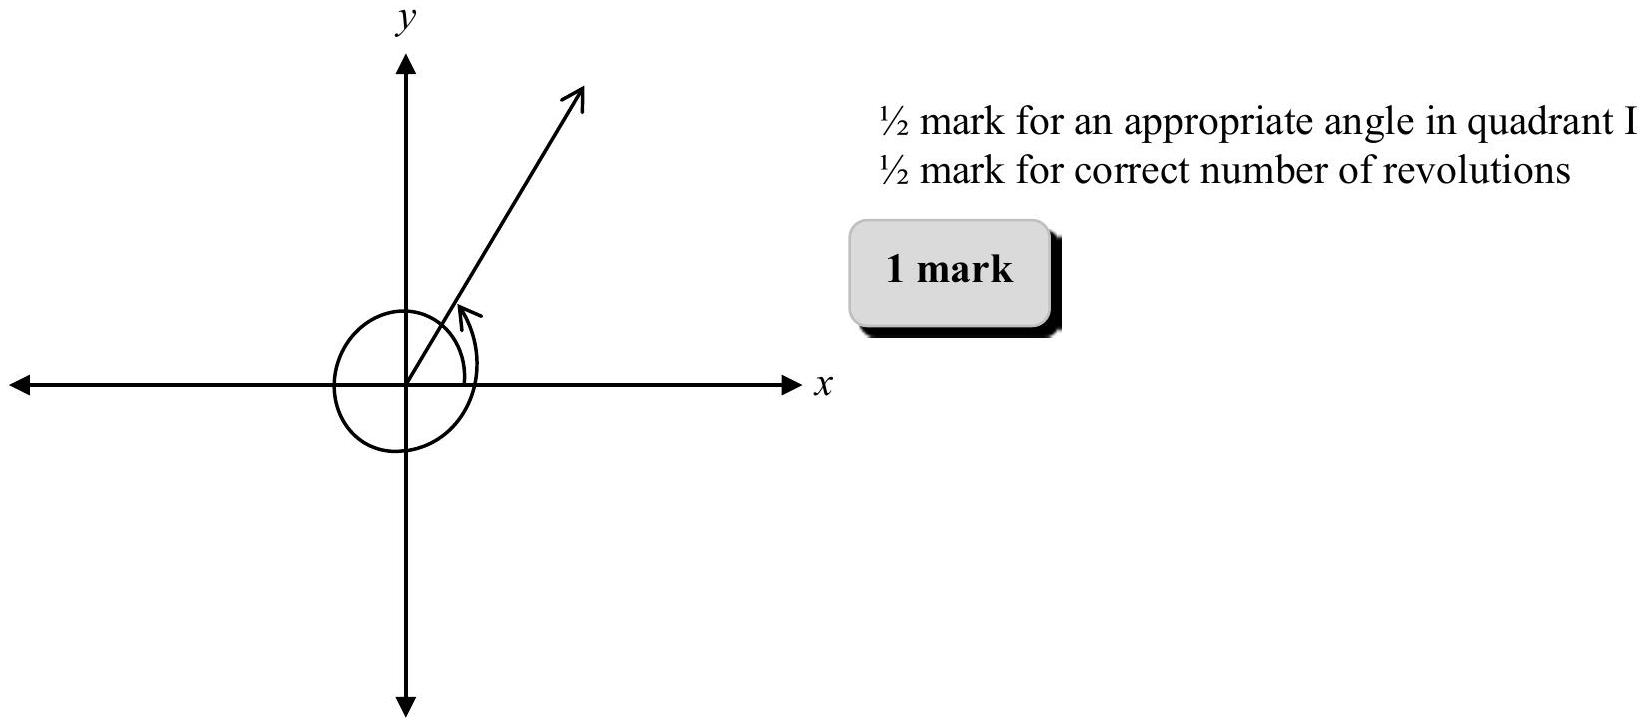
\includegraphics[max width=\textwidth, alt={}]{f67fedaf-ea11-42ad-a16e-f30d2fcf2bd3-263_727_1647_642_257}
\end{center}

Note:

\begin{itemize}
  \item If the directional arrow is not indicated, deduct an E1 error (final answer not stated).
\end{itemize}

Determine, algebraically, all of the zeros of the polynomial function $P(x)=x^{4}-5 x^{3}-4 x^{2}+20 x$.

\section*{Solution}
$P(x)=x\left(x^{3}-5 x^{2}-4 x+20\right)$\\
$P(2)=2\left(2^{3}-5(2)^{2}-4(2)+20\right) \quad 1$ mark for identifying one possible value of $x$\\
$P(2)=0$\\
$\therefore(x-2)$ is a factor

\begin{center}
\begin{tabular}{c|cccc}
2 & 1 & -5 & -4 & 20 \\
 & $\downarrow$ & 2 & -6 & -20 \\
\hline
 & 1 & -3 & -10 & 0 \\
\hline
\end{tabular}
\end{center}

1 mark for synthetic division\\
(or any other equivalent strategy)

$$
\begin{aligned}
P(x) & =x(x-2)\left(x^{2}-3 x-10\right) \\
0 & =x(x-2)(x-5)(x+2) \\
x & =0, x=2, x=5, x=-2
\end{aligned}
$$

$\frac{1}{2}$ mark for identifying all the factors\\
$\frac{1}{2}$ mark for consistent zeros\\
3 marks

Justify why four of the terms in the binomial expansion of $(-x+y)^{6}$ are positive.

\section*{Solution}
$(-x)^{6}(y)^{0},(-x)^{5}(y)^{1},(-x)^{4}(y)^{2}, \ldots$\\
$x^{6},-x^{5} y, x^{4} y^{2}, \ldots$\\
There are 7 terms. The first term is positive and the signs alternate.\\
1 mark for justification\\
1 mark

\section*{Question 9}
Determine the equation of $g(x)$ in terms of $f(x)$.\\
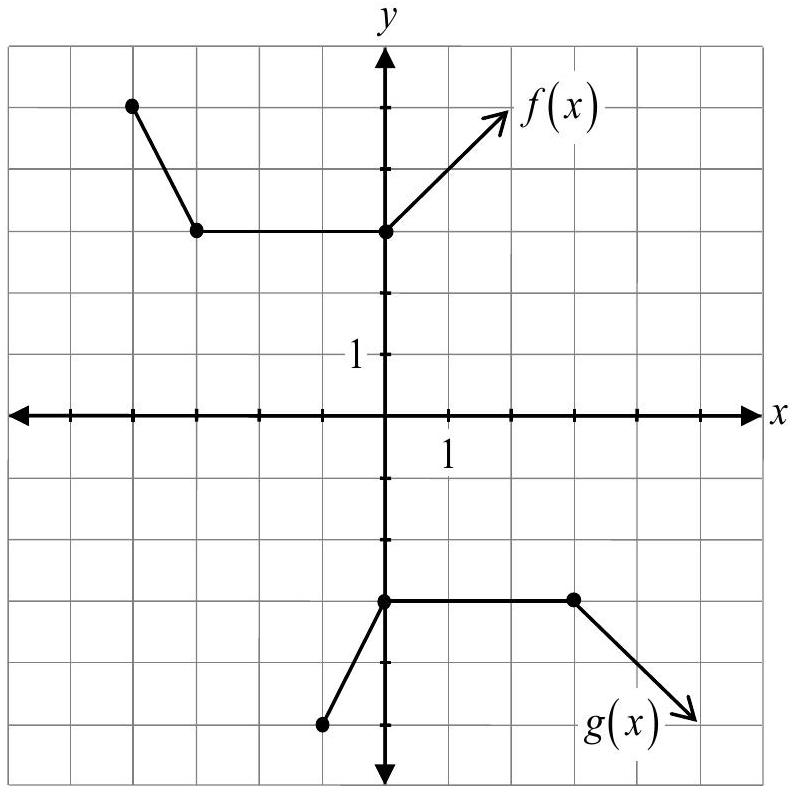
\includegraphics[max width=\textwidth, alt={}, center]{f67fedaf-ea11-42ad-a16e-f30d2fcf2bd3-266_792_794_502_674}

\section*{Solution}
$g(x)=-f(x-3)$

1 mark for vertical reflection\\
1 mark for horizontal translation

2 marks

Prove the identity for all permissible values of $x$.

$$
\frac{\sin x+\tan x}{\cot x+\csc x}=\frac{\sin ^{2} x}{\cos x}
$$

\section*{Solution}
\section*{Method 1}
\begin{center}
\begin{tabular}{|l|l|}
\hline
Left-Hand Side & Right-Hand Side \\
\hline
$\frac{\sin x+\frac{\sin x}{\cos x}}{\frac{\cos x}{\sin x}+\frac{1}{\sin x}}$ & $\frac{\sin ^{2} x}{\cos x}$ \\
\hline
$\frac{\frac{\sin x \cos x+\sin x}{\cos x}}{\frac{\cos x+1}{\sin x}}$ &  \\
\hline
$\frac{\sin x(\cos x+1)}{\cos x} \cdot \frac{\sin x}{(\cos x+1)}$ &  \\
\hline
$\frac{\sin ^{2} x}{\cos x}$ &  \\
\hline
\end{tabular}
\end{center}

1 mark for correct substitution of identities\\
1 mark for algebraic strategies\\
1 mark for logical process to prove the identity\\
3 marks

\section*{Solution}
\section*{Method 2}
\begin{center}
\begin{tabular}{|l|l|}
\hline
Left-Hand Side & Right-Hand Side \\
\hline
$\frac{\sin x+\tan x}{\frac{1}{\tan x}+\frac{1}{\sin x}}$ & $\frac{\sin ^{2} x}{\cos x}$ \\
\hline
$\frac{\frac{\sin x+\tan x}{\sin x+\tan x}}{\sin x \tan x}$ &  \\
\hline
 &  \\
\hline
\( \frac{\sin x+\tan x}{\sin x+\tan x} \cdot \sin x \tan x \) &  \\
\hline
 &  \\
\hline
\end{tabular}
\end{center}

1 mark for correct substitution of identities\\
1 mark for algebraic strategies\\
1 mark for logical process to prove the identity\\
3 marks

Given that the point $(-2,1)$ is on the graph of $y=f(x)$, describe how the coordinates of the corresponding point on the graph of $y=f(4 x)$ are different.

\section*{Solution}
The $x$-value is divided by 4 .

Using the laws of logarithms, completely expand the expression:

$$
\log \left(\frac{x^{2} \sqrt{y}}{w-1}\right)
$$

\section*{Solution}
$$
2 \log x+\frac{1}{2} \log y-\log (w-1)
$$

1 mark for product law\\
1 mark for power law ( $\frac{1}{2}$ mark for each)\\
1 mark for quotient law

3 marks

Given $\sec \theta=-\frac{5}{4}$ and $\tan \theta>0$, state the quadrant in which $\theta$ terminates.\\
Justify your answer.

\section*{Solution}
Since $\sec \theta$ is negative in quadrants II and III, and $\tan \theta$ is positive in quadrants I and III, $\theta$ terminates in quadrant III.\\
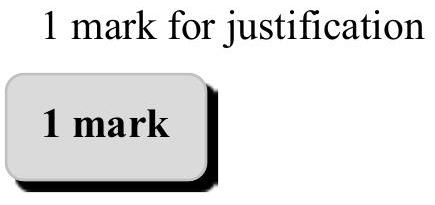
\includegraphics[max width=\textwidth, alt={}, center]{f67fedaf-ea11-42ad-a16e-f30d2fcf2bd3-271_205_435_833_936}

State an equation of a rational function that has a vertical asymptote at $x=-8$ and a horizontal asymptote at $y=9$.

\section*{Solution}
$$
y=\frac{9 x}{x+8}
$$

1 mark for vertical asymptote\\
1 mark for horizontal asymptote

\section*{2 marks}
\section*{Note:}
\begin{itemize}
  \item Other equations are possible.
\end{itemize}

Given the point $(5,1)$, state the coordinates of the corresponding point after a reflection across the line $y=x$.

\section*{Solution}
$(1,5)$ □\\
1 mark

Simplify.

$$
\frac{(n-13)!}{(n-12)!}
$$

\section*{Solution}
\begin{center}
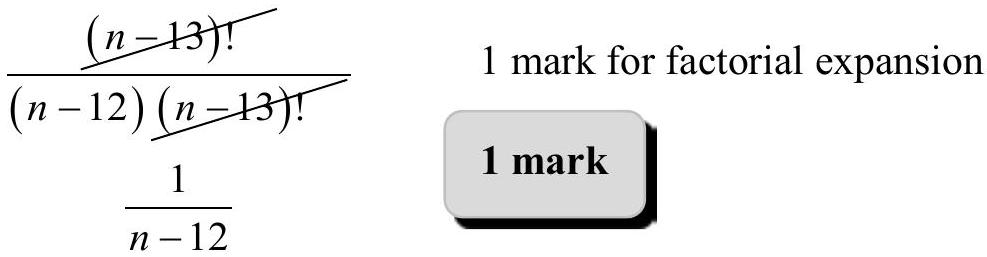
\includegraphics[max width=\textwidth, alt={}]{f67fedaf-ea11-42ad-a16e-f30d2fcf2bd3-274_257_987_708_249}
\end{center}

Given the graphs of $y=f(x)$ and $y=g(x)$,\\
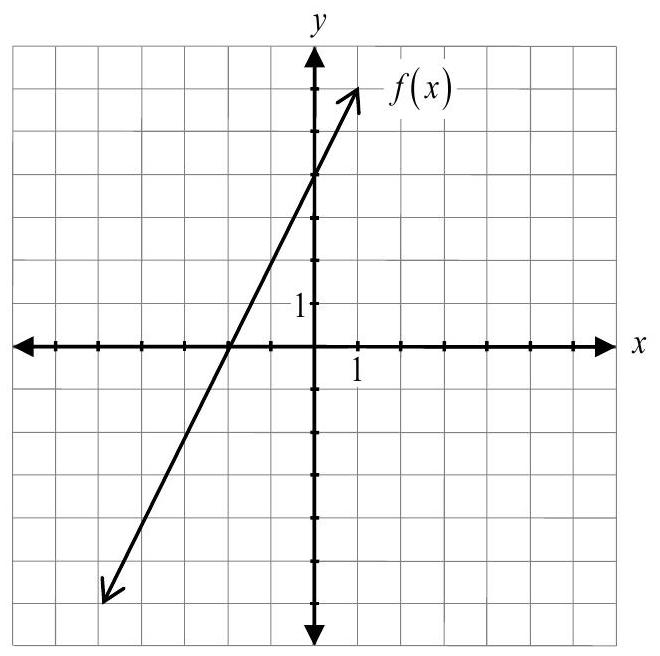
\includegraphics[max width=\textwidth, alt={}, center]{f67fedaf-ea11-42ad-a16e-f30d2fcf2bd3-275_656_660_457_378}\\
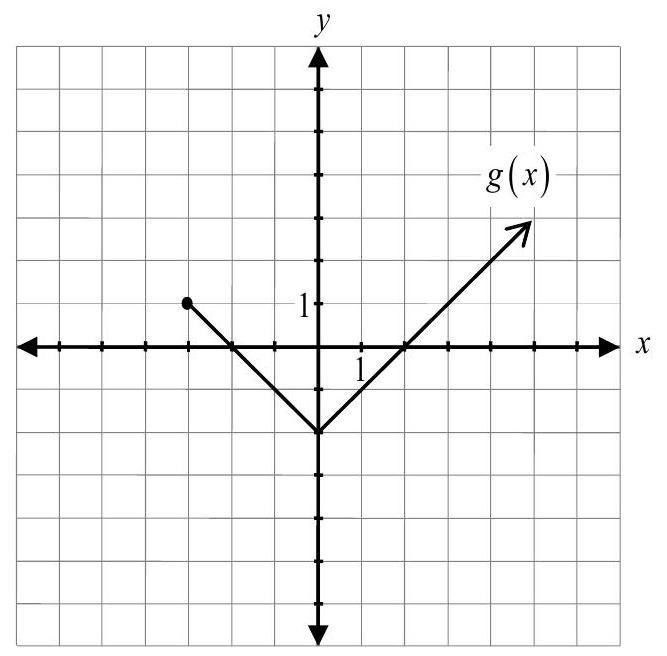
\includegraphics[max width=\textwidth, alt={}, center]{f67fedaf-ea11-42ad-a16e-f30d2fcf2bd3-275_656_667_457_1091}

\section*{Solution}
a) determine the value of $f(g(2))$.

$$
\begin{aligned}
& g(2)=0 \\
& f(0)=4
\end{aligned}
$$

$\frac{1}{2}$ mark for the value of $g(2)$\\
$\frac{1}{2}$ mark for the value of $f(g(2))$ consistent with $g(2)$

\section*{1 mark}
b) determine the value of $(g-f)(-3)$.

$$
\begin{gathered}
g(-3)-f(-3) \\
1-(-2) \\
3
\end{gathered}
$$

$\frac{1}{2}$ mark for the values of $g(-3)$ and $f(-3)$\\
$\frac{1}{2}$ mark for value of $(g-f)(-3)$ consistent with $g(-3)$ and $f(-3)$

1 mark

Identify the remainder when $P(x)=3 x^{3}-x^{2}+1$ is divided by $(x-2)$.\\
a) -27\\
b) -19\\
c) 11\\
d) 21

\section*{Question 19}
Identify the logarithmic form of $2^{x}=\frac{1}{4}$.\\
a) $\log _{2} x=\frac{1}{4}$\\
b) $\log _{x} 2=\frac{1}{4}$\\
c) $\log _{2}\left(\frac{1}{4}\right)=x$\\
d) $\log _{x}\left(\frac{1}{4}\right)=2$

Question 20

Leah's Pizzeria offers 9 different pizza toppings. Identify the expression that represents the number of different types of pizzas, with 3 different toppings, that can be made.\\
a) ${ }_{9} C_{3}$\\
b) ${ }_{9} P_{3}$\\
c) $\frac{9!}{3!}$\\
d) $9!3!$

Given $(5,-4)$ is a point on the graph of $y=f(x)$, identify the corresponding point on the graph of $y=\frac{1}{f(x)}$.\\
a) $\left(\frac{1}{5},-4\right)$\\
b) $\left(5,-\frac{1}{4}\right)$\\
c) $\left(\frac{1}{5},-\frac{1}{4}\right)$\\
d) $(-4,5)$

Question 22

Identify the non-permissible value of $x$ for $1+\sec x$ over $[0, \pi]$.\\
a) 0\\
b) $\frac{\pi}{4}$\\
c) $\frac{\pi}{2}$\\
d) $\pi$

Question 23

Indicate the combination that represents the circled term in the given row of Pascal's triangle.\\
1\\
46\\
(4) 1\\
a) ${ }_{4} C_{3}$\\
b) ${ }_{4} C_{4}$\\
c) ${ }_{5} C_{3}$\\
d) ${ }_{5} \mathrm{C}_{4}$

Identify the $x$-intercept on the graph of $f(x)=\sqrt{2(x+5)}$.\\
a) -5\\
b) 0\\
c) $\sqrt{10}$\\
d) 5

\section*{Question 25}
Identify the coterminal angle of $\frac{\pi}{5}$ over the interval $-\pi \leq \theta \leq 4 \pi$.\\
a) $-\frac{9 \pi}{5}$\\
b) $-\frac{\pi}{5}$\\
c) $\frac{3 \pi}{5}$\\
d) $\frac{11 \pi}{5}$

\section*{Question 26}
Given $f(x)=\{(2,6),(3,2),(3,4),(6,5)\}$, identify the value of $f(f(2))$.\\
a) 3\\
b) 4\\
c) 5\\
d) 6

The graph of $f(x)=(x-1)^{2}$ is translated 2 units to the left and 3 units up. Identify the equation of the transformed graph, $g(x)$.\\
a) $g(x)=(x+1)^{2}+3$\\
b) $g(x)=(x-3)^{2}+3$\\
c) $g(x)=(x+2)^{2}+3$\\
d) $g(x)=(x-2)^{2}+3$

Given $\csc \theta=-\frac{8}{5}$, determine the exact value of $\cos 2 \theta$.

\section*{Solution}
$$
\begin{aligned}
\cos 2 \theta & =1-2 \sin ^{2} \theta \\
& =1-2\left(-\frac{5}{8}\right)^{2} \quad
\end{aligned} \quad \begin{aligned}
& 1 \text { mark for the value of } \sin \theta \\
& 1 \text { mark for substitution into correct identity }
\end{aligned}
$$

Determine the period of the sinusoidal function, $f(x)=-6 \cos \left(\frac{\pi}{6}(x+1)\right)+5$.

\section*{Solution}
$$
\begin{aligned}
\text { Period } & =\frac{2 \pi}{\left(\frac{\pi}{6}\right)} \\
& =12
\end{aligned}
$$

□

Determine, algebraically, the equation of $P(x)$, given the graph of the polynomial function $P(x)$.\\
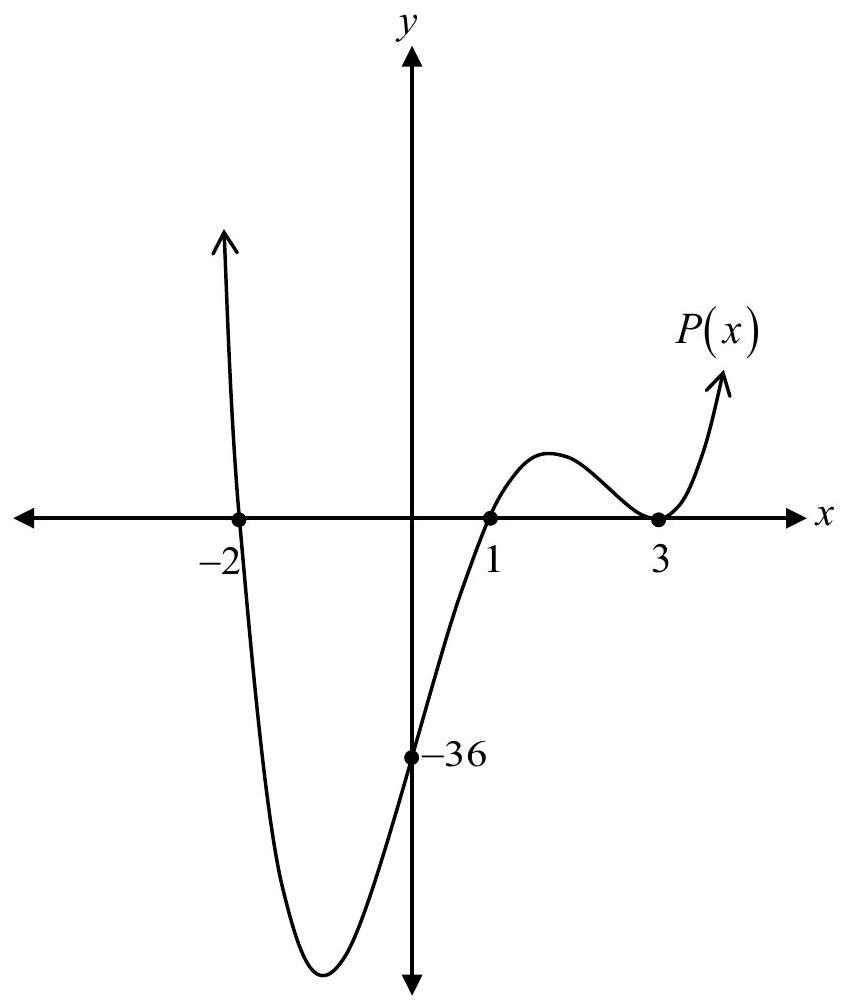
\includegraphics[max width=\textwidth, alt={}, center]{f67fedaf-ea11-42ad-a16e-f30d2fcf2bd3-282_1005_847_489_623}

\section*{Solution}
$$
\begin{aligned}
P(x) & =a(x-3)^{2}(x-1)(x+2) & & \frac{1}{2} \text { mark for factors of } P(x) \\
-36 & =a(-3)^{2}(-1)(2) & & 1 / 2 \text { mark for multiplicity of } 2 \text { at } x=3 \\
-36 & =-18 a & & 1 / 2 \text { mark for substitution of } P(0)=-36 \\
a & =2 & & 1 / 2 \text { mark for correct value of } a \\
P(x) & =2(x-3)^{2}(x-1)(x+2) & & \mathbf{2} \text { marks }
\end{aligned}
$$

Solve $2 \sin ^{2} \theta-7 \sin \theta-4=0$ where $\theta \in \mathbb{R}$.

\section*{Solution}
$$
\begin{array}{ll}
(2 \sin \theta+1)(\sin \theta-4)=0 & \\
\sin \theta=-\frac{1}{2} \quad \sin \theta=4 & 1 \text { mark for solving for } \sin \theta\left(\frac{1}{2} \text { mark for each branch }\right) \\
\theta=\frac{7 \pi}{6}, \frac{11 \pi}{6} \quad \text { No solution } & 2 \text { marks for solving for } \theta(1 \text { mark for each branch }) \\
\theta=\frac{7 \pi}{6}+2 k \pi, k \in \mathbb{Z} & \\
\theta=\frac{11 \pi}{6}+2 k \pi, k \in \mathbb{Z} & 1 \text { mark for general solution }
\end{array}
$$

Justify that the shapes of the graphs of $f(x)=(x+1)^{2}(x-1)$ and $g(x)=(x+1)^{2}(x-1)^{3}$ are different as they approach the $x$-intercept at $x=1$.

\section*{Solution}
At $x=1$, both graphs pass through the $x$-axis, however, the graph of $g(x)$ flattens as it passes through the $x$-axis.

Determine the exact value of $\cot \theta$ if $\cos \theta=-\frac{4}{7}$ and $\sin \theta$ is positive.

\section*{Solution}
$x^{2}+y^{2}=r^{2}$\\
$(-4)^{2}+y^{2}=(7)^{2} \quad 1 / 2$ mark for substitution\\
$y^{2}=49-16$\\
$y= \pm \sqrt{33} \quad 1 / 2$ mark for solving for $y$\\
$\cot \theta=\frac{-4}{\sqrt{33}} \quad 1$ mark for consistent value of $\cot \theta\left(\frac{1}{2}\right.$ mark for quadrant; $\frac{1}{2}$ mark for value $)$\\
or\\
2 marks\\
$\cot \theta=\frac{-4 \sqrt{33}}{33}$

Note:

\begin{itemize}
  \item Accept any of the following values for $y: y= \pm \sqrt{33}, y=\sqrt{33}$, or $y=-\sqrt{33}$.
\end{itemize}

Sketch the graph of $f(x)=-\log _{2}(x)+2$.

\section*{Solution}
\begin{center}
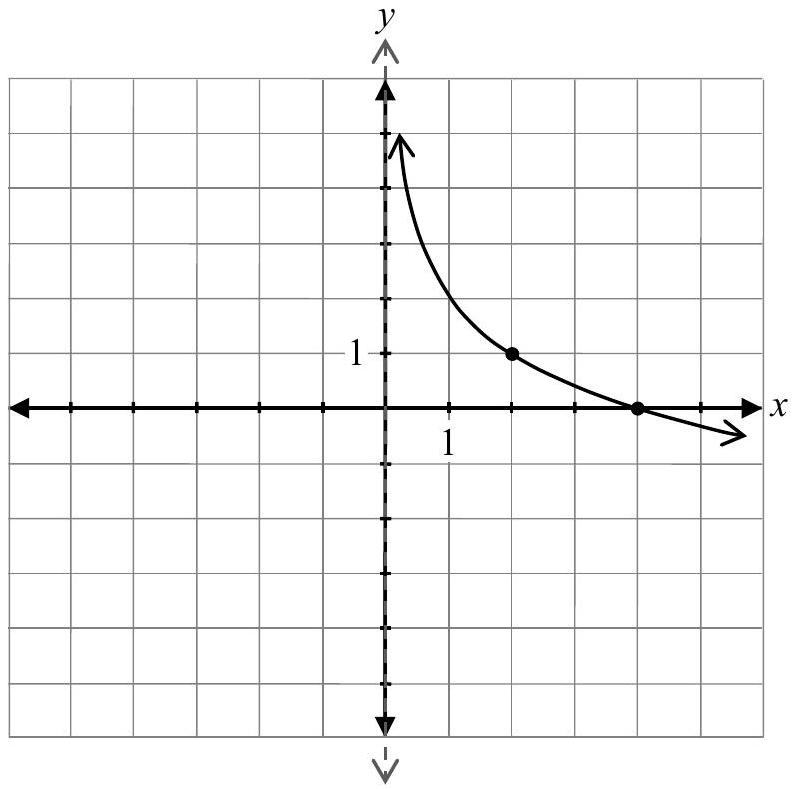
\includegraphics[max width=\textwidth, alt={}]{f67fedaf-ea11-42ad-a16e-f30d2fcf2bd3-286_789_796_567_257}
\end{center}

1 mark for asymptotic behaviour approaching $x=0$\\
1 mark for vertical reflection\\
1 mark for vertical translation

3 marks

State the range of $f(x)=\sqrt{x+4}$.

\section*{Solution}
Range: $[0, \infty)$\\
or

Range: $\{y \in \mathbb{R} \mid y \geq 0\}$

Sophie correctly solved the logarithmic equation, $\log _{7}(x-1)=\log _{7}(2 x-2)$.

$$
\begin{aligned}
x-1 & =2 x-2 \\
-1+2 & =2 x-x
\end{aligned}
$$

Explain why $x=1$ is an extraneous root.

\section*{Solution}
The root, $x=1$, is an extraneous root because the argument of a logarithm cannot be zero.\\

\includegraphics[max width=\textwidth, alt={}, center]{f67fedaf-ea11-42ad-a16e-f30d2fcf2bd3-288_134_226_1196_988}

Sketch the graph of $f(x)=\sqrt{4 x}-1$.

\section*{Solution}
\begin{center}
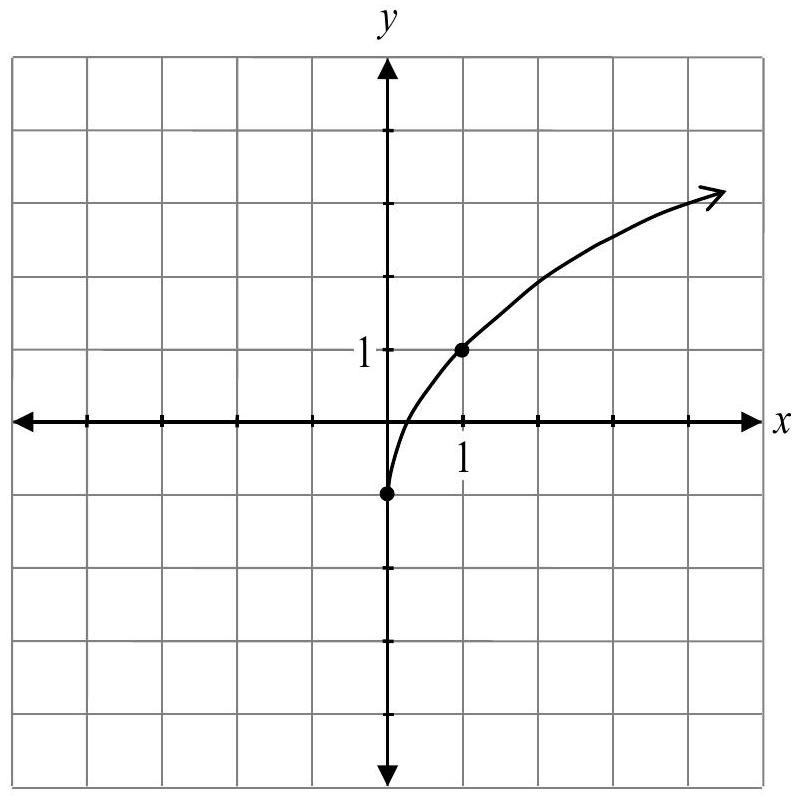
\includegraphics[max width=\textwidth, alt={}]{f67fedaf-ea11-42ad-a16e-f30d2fcf2bd3-289_798_802_580_249}
\end{center}

1 mark for shape of a radical function 1 mark for horizontal compression 1 mark for vertical translation

3 marks

Solve, algebraically.

$$
{ }_{n} C_{2}=2 n+7
$$

\section*{Solution}
$$
\begin{aligned}
\frac{n!}{(n-2)!2!} & =2 n+7 & & 1 / 2 \text { mark for substitution into equation } \\
\frac{n(n-1)(n-2)!}{(n-2)!} & =2!(2 n+7) & & \begin{array}{l}
1 / 2 \text { mark for factorial expansion } \\
1 / 2 \text { mark for simplification of factorial }
\end{array} \\
n(n-1) & =2(2 n+7) & & \\
n^{2}-n & =4 n+14 & & \\
n^{2}-5 n-14 & =0 & & 1 / 2 \text { mark for simplification } \\
(n+2)(n-7) & =0 & & 1 / 2 \text { mark for the permissible value of } n \\
n \geq-2 \quad n & =7 & & 1 / 2 \text { mark for showing the rejection of the extraneous root }
\end{aligned}
$$

Given $f(x)=x^{2}-1$ and $g(x)=x-3$, explain why the domain of $h(x)=\frac{f(x)}{g(x)}$ has a restriction when $x=3$.

\section*{Solution}
When $x=3$, the denominator is equal to zero and it is not possible to divide by zero.

1 mark

Evaluate.

$$
\frac{\cot \left(\frac{11 \pi}{6}\right) \sin \left(-\frac{4 \pi}{3}\right)}{\cos \left(\frac{2 \pi}{3}\right)}
$$

\section*{Solution}
$\frac{(-\sqrt{3})\left(\frac{\sqrt{3}}{2}\right)}{-\frac{1}{2}}$\\
1 mark for $\cot \left(\frac{11 \pi}{6}\right)\left(\frac{1}{2}\right.$ mark for quadrant; $\frac{1}{2}$ mark for value)\\
1 mark for $\sin \left(-\frac{4 \pi}{3}\right)\left(\frac{1}{2}\right.$ mark for quadrant; $1 / 2$ mark for value $)$\\
1 mark for $\cos \left(\frac{2 \pi}{3}\right)$ ( $\frac{1}{2}$ mark for quadrant; $1 / 2$ mark for value)\\
$\left(-\frac{3}{2}\right)\left(-\frac{2}{1}\right)$\\
3 marks

3

Solve, algebraically.

$$
\log _{2}\left(\log _{3} x\right)=2
$$

\section*{Solution}
$2^{2}=\log _{3} x \frac{1}{2}$ mark for exponential form\\
$4=\log _{3} x$\\
$x=3^{4}$\\
$\frac{1}{2}$ mark for exponential form\\
$x=81$

Sketch the graph of the function $y=5 \sin \left(\frac{\pi}{4} x\right)+1$ over the domain $[-4,8]$.

\section*{Solution}
\begin{center}
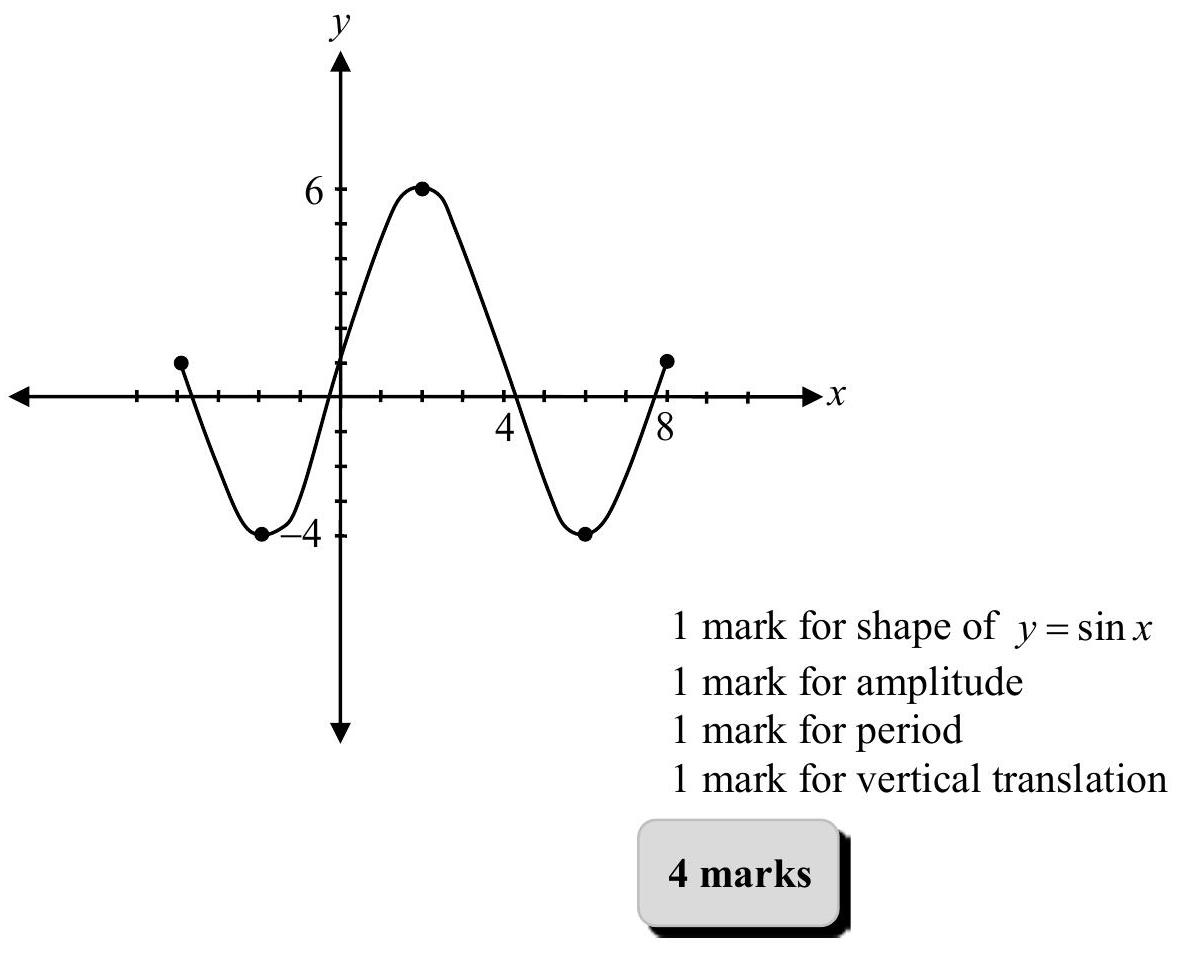
\includegraphics[max width=\textwidth, alt={}]{f67fedaf-ea11-42ad-a16e-f30d2fcf2bd3-294_953_1191_648_412}
\end{center}

Given the graph of $y=f(x)$, sketch the graph of $y=|f(-x)|$.\\
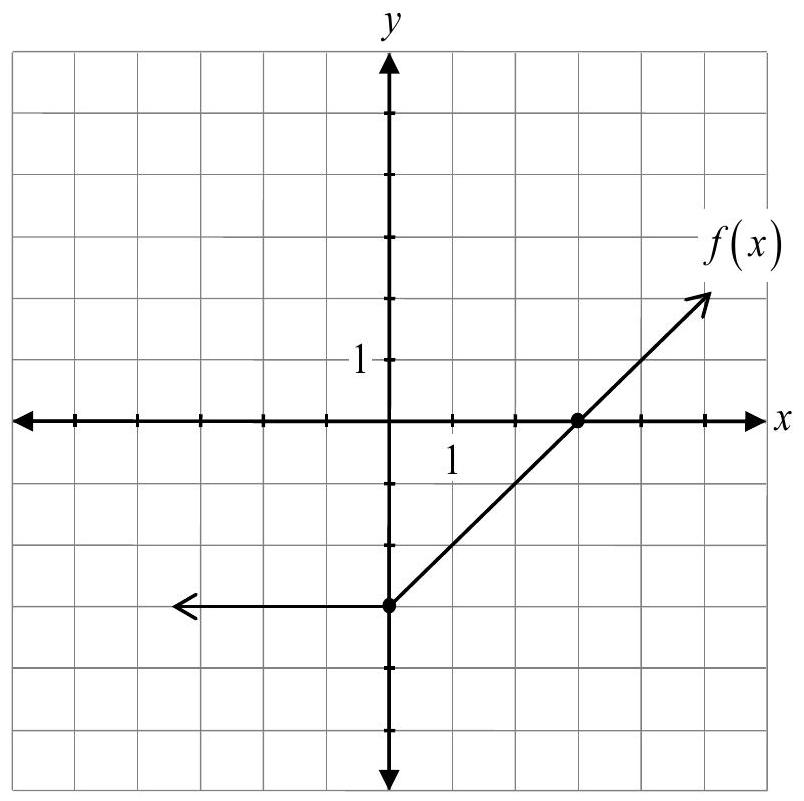
\includegraphics[max width=\textwidth, alt={}, center]{f67fedaf-ea11-42ad-a16e-f30d2fcf2bd3-295_801_804_534_711}

\section*{Solution}
\begin{center}
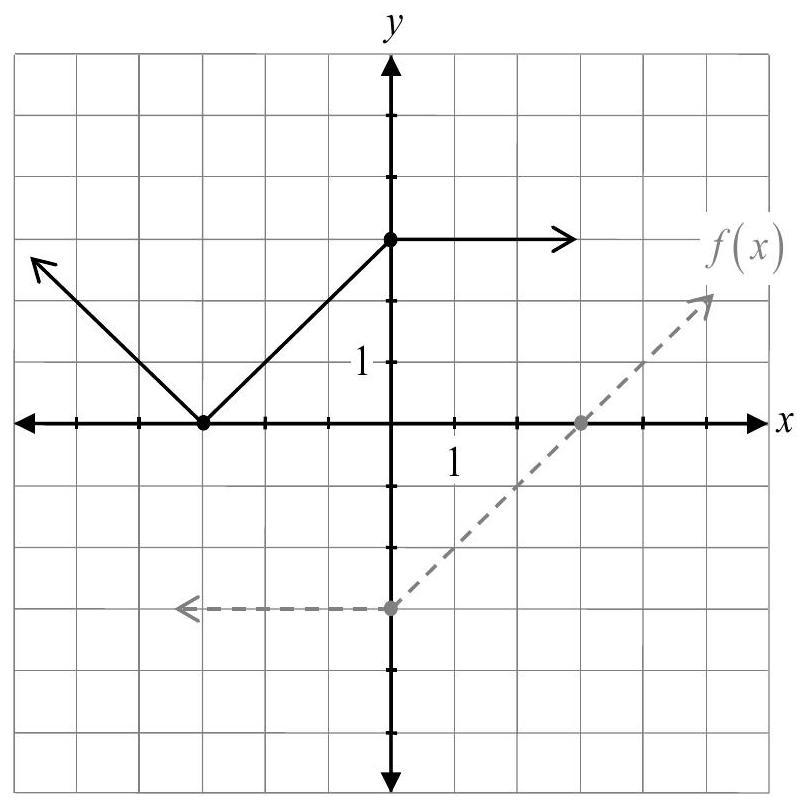
\includegraphics[max width=\textwidth, alt={}]{f67fedaf-ea11-42ad-a16e-f30d2fcf2bd3-295_806_809_1435_259}
\end{center}

1 mark for horizontal reflection 1 mark for absolute value

2 marks

Savannah used the graph of $y=f(x)$ to sketch the graph of $y=\sqrt{f(x)}$. Her solution is given below. Describe her error.\\
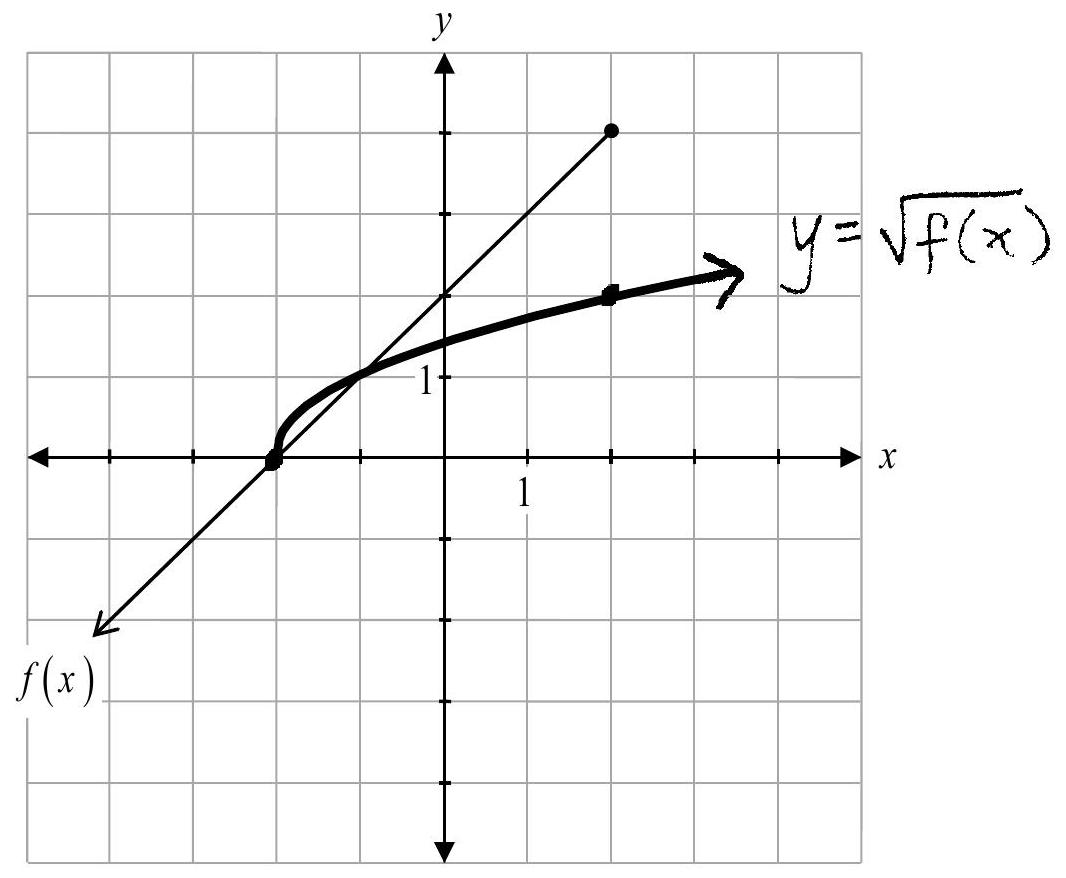
\includegraphics[max width=\textwidth, alt={}, center]{f67fedaf-ea11-42ad-a16e-f30d2fcf2bd3-296_878_1066_620_554}

\section*{Solution}
Savannah did not restrict the domain at $x=2$.

Determine the exact value of $\sin \left(\frac{13 \pi}{12}\right)$.

\section*{Solution}
$\sin \left(\frac{3 \pi}{4}+\frac{\pi}{3}\right)=\sin \left(\frac{3 \pi}{4}\right) \cos \left(\frac{\pi}{3}\right)+\cos \left(\frac{3 \pi}{4}\right) \sin \left(\frac{\pi}{3}\right)$

$$
\begin{aligned}
& =\left(\frac{\sqrt{2}}{2}\right)\left(\frac{1}{2}\right)+\left(-\frac{\sqrt{2}}{2}\right)\left(\frac{\sqrt{3}}{2}\right) \\
& =\frac{\sqrt{2}}{4}-\frac{\sqrt{6}}{4} \\
& =\frac{\sqrt{2}-\sqrt{6}}{4}
\end{aligned}
$$

1 mark for substitution into correct identity 2 marks ( $\frac{1}{2}$ mark for each exact value)

Note:

\begin{itemize}
  \item Other combinations are possible.
\end{itemize}

State the equation of the horizontal asymptote of $f(x)=\frac{3 x}{x-1}$.

\section*{Solution}
$y=3 \quad \mathbf{1}$ mark

Sketch the graph of $f(x)=\frac{5 x-10}{x^{2}+x-6}$.

\section*{Solution}
$$
\begin{aligned}
f(x) & =\frac{5 x-10}{x^{2}+x-6} \\
& =\frac{5(x-2)}{(x-2)(x+3)} \\
& =\frac{5}{x+3}, x \neq 2
\end{aligned}
$$

∴ there is a point of discontinuity (hole) at $(2,1)$\\
vertical asymptote at $x=-3$\\
horizontal asymptote at $y=0$\\
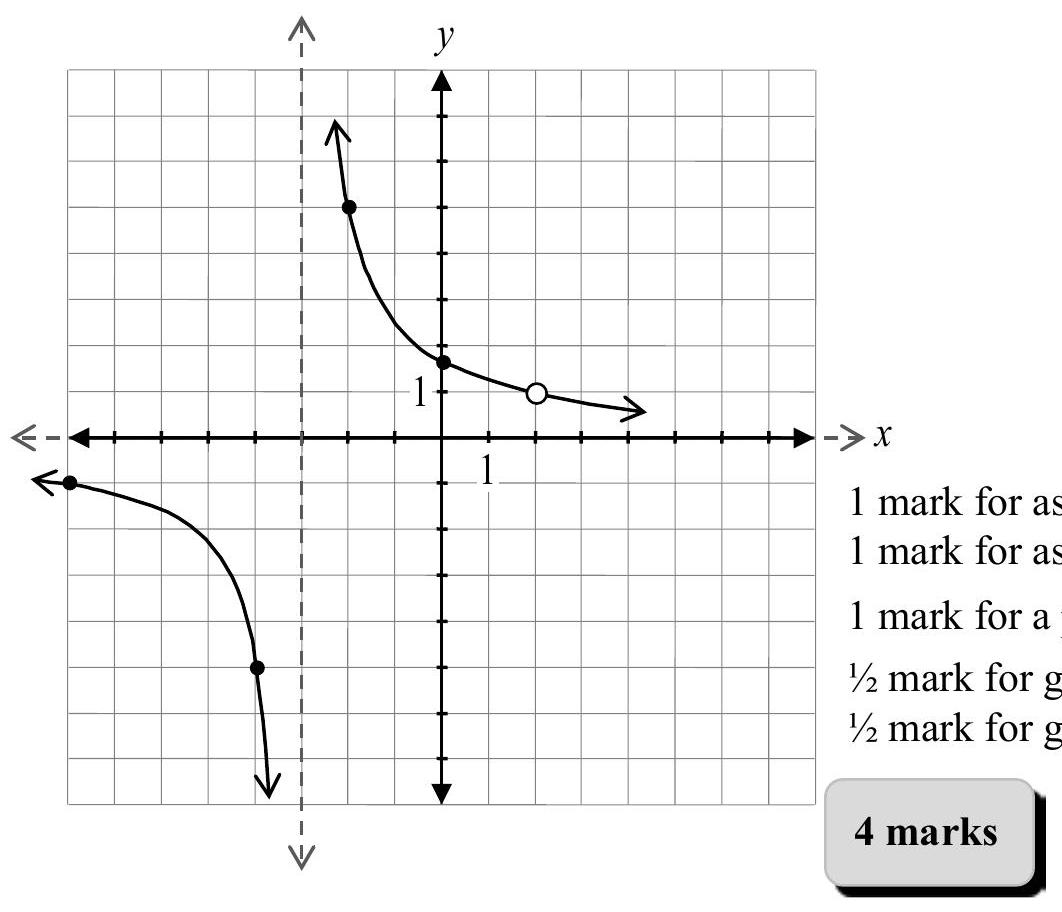
\includegraphics[max width=\textwidth, alt={}, center]{f67fedaf-ea11-42ad-a16e-f30d2fcf2bd3-299_912_1062_1316_208}

Determine, algebraically, the inverse of $f(x)=3 x+4$.

\section*{Solution}
Let $f(x)=y$\\
$y=3 x+4$\\
$x=3 y+4$\\
1 mark for switching $x$ and $y$-values\\
$x-4=3 y$\\
$\frac{x-4}{3}=y$\\
$\frac{1}{2}$ mark for solving for $y$\\
$f^{-1}(x)=\frac{x-4}{3}$\\
$\frac{1}{2}$ mark for writing equation of $f^{-1}(x)$\\
2 marks

Sketch the graph of $P(x)=-(x+1)(x-2)(x+3)$.

\section*{Solution}
\begin{center}
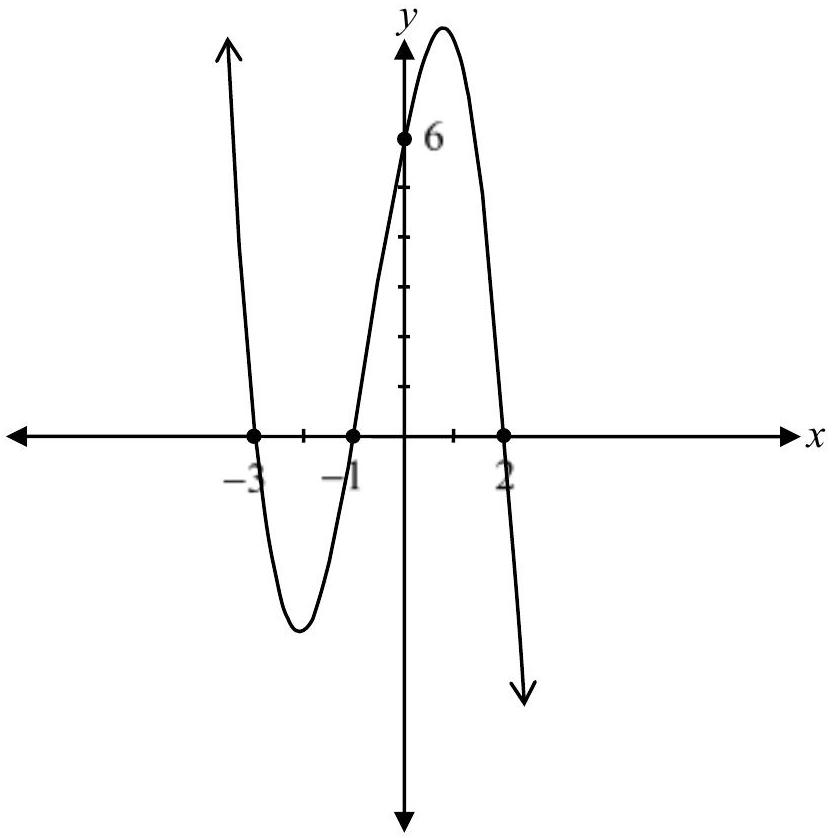
\includegraphics[max width=\textwidth, alt={}]{f67fedaf-ea11-42ad-a16e-f30d2fcf2bd3-301_838_833_580_244}
\end{center}

1 mark for $x$-intercepts\\
$\frac{1}{2}$ mark for $y$-intercept\\
$\frac{1}{2}$ mark for end behaviour\\
2 marks

Determine and simplify the $8^{\text {th }}$ term in the binomial expansion of $\left(x-\frac{2}{x^{3}}\right)^{10}$.

\section*{Solution}
$$
\begin{array}{rlr}
t_{8} & ={ }_{10} C_{7}(x)^{3}\left(-\frac{2}{x^{3}}\right)^{7} & 2 \text { marks (1 mark for }{ }_{10} C_{7} ; 1 / 2 \text { mark for each consistent factor) } \\
& =120\left(x^{3}\right)\left(-\frac{128}{x^{21}}\right) & \\
& =-\frac{15360}{x^{18}} & 1 \text { mark for simplification }(1 / 2 \text { mark for coefficient; } 1 / 2 \text { mark for exponent })
\end{array}
$$

The temperature of hot chocolate is recorded as it cools down. The data shows that the temperature cools according to the equation:

$$
T=82(0.87)^{t}+16
$$

where $T$ is the temperature of the hot chocolate, in degrees Celsius after $t$ minutes and $t$ is the time, in minutes, after the hot chocolate is made.

In order to avoid burns, hot chocolate should not be served at a temperature higher than $71^{\circ} \mathrm{C}$. Determine, algebraically, the amount of time it will take the hot chocolate to reach this temperature.

\section*{Solution}
$$
\begin{aligned}
71 & =82(0.87)^{t}+16 \\
55 & =82(0.87)^{t} \\
\frac{55}{82} & =0.87^{t} \\
\log \left(\frac{55}{82}\right) & =t \log (0.87) \quad \begin{array}{l}
1 / 2 \text { mark for applying logarithms } \\
1 \text { mark for power law }
\end{array} \\
t & =\frac{\log \left(\frac{55}{82}\right)}{\log (0.87)} \\
t & =2.867874 \\
t & =2.868 \text { minutes } \quad 1 / 2 \text { mark for evaluating quotient of logarithms }
\end{aligned}
$$

Solve for $\theta$, algebraically, over the interval $[0,2 \pi]$.

$$
3 \sin ^{2} \theta+6 \sin \theta+2=0
$$

\section*{Solution}
$$
\begin{aligned}
& \sin \theta=\frac{-6 \pm \sqrt{6^{2}-4(3)(2)}}{2(3)} \quad \frac{1}{2} \text { mark for substitution into quadratic formula } \\
& \sin \theta=\frac{-6 \pm \sqrt{12}}{6} \\
& \frac{1}{2} \text { mark for solving for } \sin \theta \\
& \sin \theta=-0.422649 \ldots \quad \sin \theta=-1.577350 \ldots \\
& \theta_{r}=0.436367 \ldots \text { no solution }
\end{aligned}
$$

2 marks for solving for $\theta$\\
( $\frac{1}{2}$ mark for each value; 1 mark for indicating no solution)

A committee of 4 people is to be selected from 6 high school students and 5 middle years students.

Determine the number of possible committees if the committee must have at least 3 high school students.

\section*{Solution}
Case 1: ${ }_{6} C_{3} \cdot{ }_{5} C_{1}=100$\\
1 mark for Case 1\\
Case 2: ${ }_{6} C_{4} \cdot{ }_{5} C_{0}=15$\\
1 mark for Case 2\\
$100+15=115$ possible committees\\
1 mark for addition of cases\\
3 marks

Note:

\begin{itemize}
  \item ${ }_{5} C_{0}$ does not need to be shown.
\end{itemize}

Given the graph of $y=f(x)$, sketch the graph of $y=-|f(x)|$.

\section*{Solution}
\begin{center}
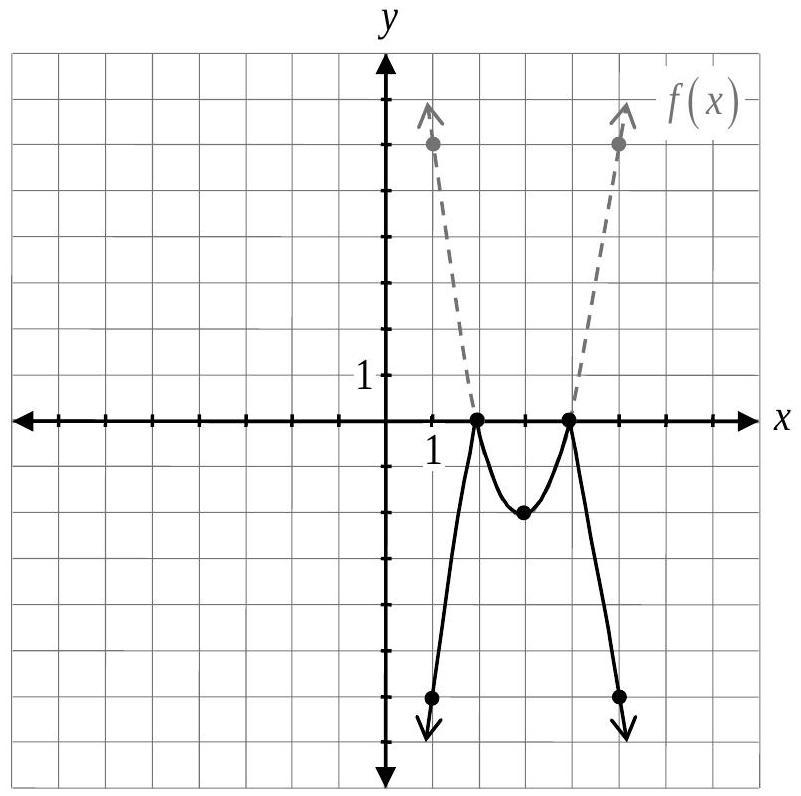
\includegraphics[max width=\textwidth, alt={}]{f67fedaf-ea11-42ad-a16e-f30d2fcf2bd3-306_796_801_554_259}
\end{center}

1 mark for absolute value 1 mark for vertical reflection

2 marks

Describe the transformations used to obtain the graph of the function $y=4 f\left(\frac{x}{2}\right)-3$ from the graph of $y=f(x)$.

\section*{Solution}
The graph of $y=f(x)$ is vertically stretched by a factor of 4, horizontally stretched by a factor of 2 , and translated down 3 units.

1 mark for vertical stretch\\
1 mark for horizontal stretch\\
1 mark for vertical translation\\
3 marks

Note:

\begin{itemize}
  \item Deduct a maximum of 1 mark for concept error of incorrect order of vertical transformations.
\end{itemize}

If $\log 4=m$ and $\log 3=n$, express $\log 48$ in terms of $m$ and $n$.

\section*{Solution}
$$
\begin{array}{rlr}
\log 48 & =\log \left(4^{2} \cdot 3\right) & \\
& =2 \log 4+\log 3 & \\
& =2 m+n &
\end{array} \text { 1 mark for power law } \text { for product law } \text { }
$$

2 marks

State the domain and range of the radical function, $f(x)=-3 \sqrt{x-8}+1$.

\section*{Solution}
\begin{center}
\begin{tabular}{lc}
Domain: $[8, \infty)$ & 1 mark for domain \\
Range: $[(-\infty, 1]$ & 1 mark for range \\
 & $\mathbf{2}$ marks \\
\end{tabular}
\end{center}

Explain why the graph of $y=\tan x$ does not have an amplitude.

\section*{Solution}
The range of $y=\tan x$ is all real numbers.\\
or\\
As the graph of $y=\tan x$ approaches the vertical asymptotes, the function value approaches positive and negative infinity.

Prove the following identity for all permissible values of $\theta$.

$$
\frac{\sec \theta-\sin ^{2} \theta \sec \theta}{\tan \theta \sin \theta}=\csc ^{2} \theta-1
$$

\section*{Solution}
\section*{Method 1}
\begin{center}
\begin{tabular}{|l|l|}
\hline
Left-Hand Side & Right-Hand Side \\
\hline
$\frac{\frac{1}{\cos \theta}-\frac{\sin ^{2} \theta}{\cos \theta}}{\left(\frac{\sin \theta}{\cos \theta}\right)(\sin \theta)}$ & $\csc ^{2} \theta-1$ \\
\hline
$\frac{\frac{1-\sin ^{2} \theta}{\cos \theta}}{\frac{\sin ^{2} \theta}{\cos \theta}}$ &  \\
\hline
$\frac{\cos ^{2} \theta}{\sin ^{2} \theta}$ &  \\
\hline
$\cot ^{2} \theta$ &  \\
\hline
$\csc ^{2} \theta-1$ &  \\
\hline
\end{tabular}
\end{center}

1 mark for correct substitution of appropriate identities\\
1 mark for algebraic strategies\\
1 mark for logical process to prove the identity\\
3 marks

\section*{Method 2}
\begin{center}
\begin{tabular}{|l|l|}
\hline
Left-Hand Side & Right-Hand Side \\
\hline
$\frac{\sec \theta\left(1-\sin ^{2} \theta\right)}{\left(\frac{\sin \theta}{\cos \theta}\right)(\sin \theta)}$ & $\csc ^{2} \theta-1$ \\
\hline
$\frac{\left(\frac{1}{\cos \theta}\right)\left(\cos ^{2} \theta\right)}{\frac{\sin ^{2} \theta}{\cos \theta}}$ &  \\
\hline
$\frac{\frac{\cos ^{2} \theta}{\cos \theta}}{\frac{\sin ^{2} \theta}{\cos \theta}}$ &  \\
\hline
\( \cot ^{2} \theta \) &  \\
\hline
$\csc ^{2} \theta-1$ &  \\
\hline
\end{tabular}
\end{center}

1 mark for correct substitution of appropriate identities\\
1 mark for algebraic strategies\\
1 mark for logical process to prove the identity

3 marks

Given that $x=3$ is one of the zeros of $p(x)=x^{3}-7 x-6$, express $p(x)$ in completely factored form.

\section*{Solution}
\begin{center}
\begin{tabular}{l|rrrr}
3 & 1 & 0 & -7 & -6 \\
 &  & 3 & 9 & 6 \\
\hline
 & 1 & 3 & 2 & 0 \\
\hline
\end{tabular}
\end{center}

1 mark for synthetic division (or equivalent strategy)\\
$p(x)=(x-3)\left(x^{2}+3 x+2\right) \frac{1}{2}$ mark for factor of $(x-3)$\\
$p(x)=\underline{(x-3)(x+2)(x+1)} \frac{1}{2}$ mark for other consistent factors

2 marks

Solve, algebraically.

$$
{ }_{n+1} P_{2}=6
$$

\section*{Solution}
$$
\begin{aligned}
\frac{(n+1)!}{(n+1-2)!} & =6 \quad 1 / 2 \text { mark for substitution } \\
\frac{(n+1)!}{(n-1)!} & =6
\end{aligned}
$$

$\frac{(n+1)(n)(n-1)!}{(n-1)!}=6$

$$
\begin{aligned}
n^{2}+n & =6 \\
n^{2}+n-6 & =0 \\
(n+3)(n-2) & =0 \\
n \geq-3 \quad n & =2
\end{aligned}
$$

1 mark for factorial expansion\\
$\frac{1}{2}$ mark for simplification of factorials\\
$\frac{1}{2}$ mark for the permissible value of $n$\\
$\frac{1}{2}$ mark for showing the rejection of the extraneous root

\section*{3 marks}
Express $\log (3 x-1)-\log x+\log 9$ as a single logarithm.

\section*{Solution}
$$
\begin{array}{ll}
\log \left(\frac{9(3 x-1)}{x}\right) & 1 \text { mark for product law } \\
& 1 \text { mark for quotient law } \\
& \mathbf{2} \text { marks }
\end{array}
$$

Sketch the graph of $P(x)=-(x-2)^{2}(x+3)$.

\section*{Solution}
\begin{center}
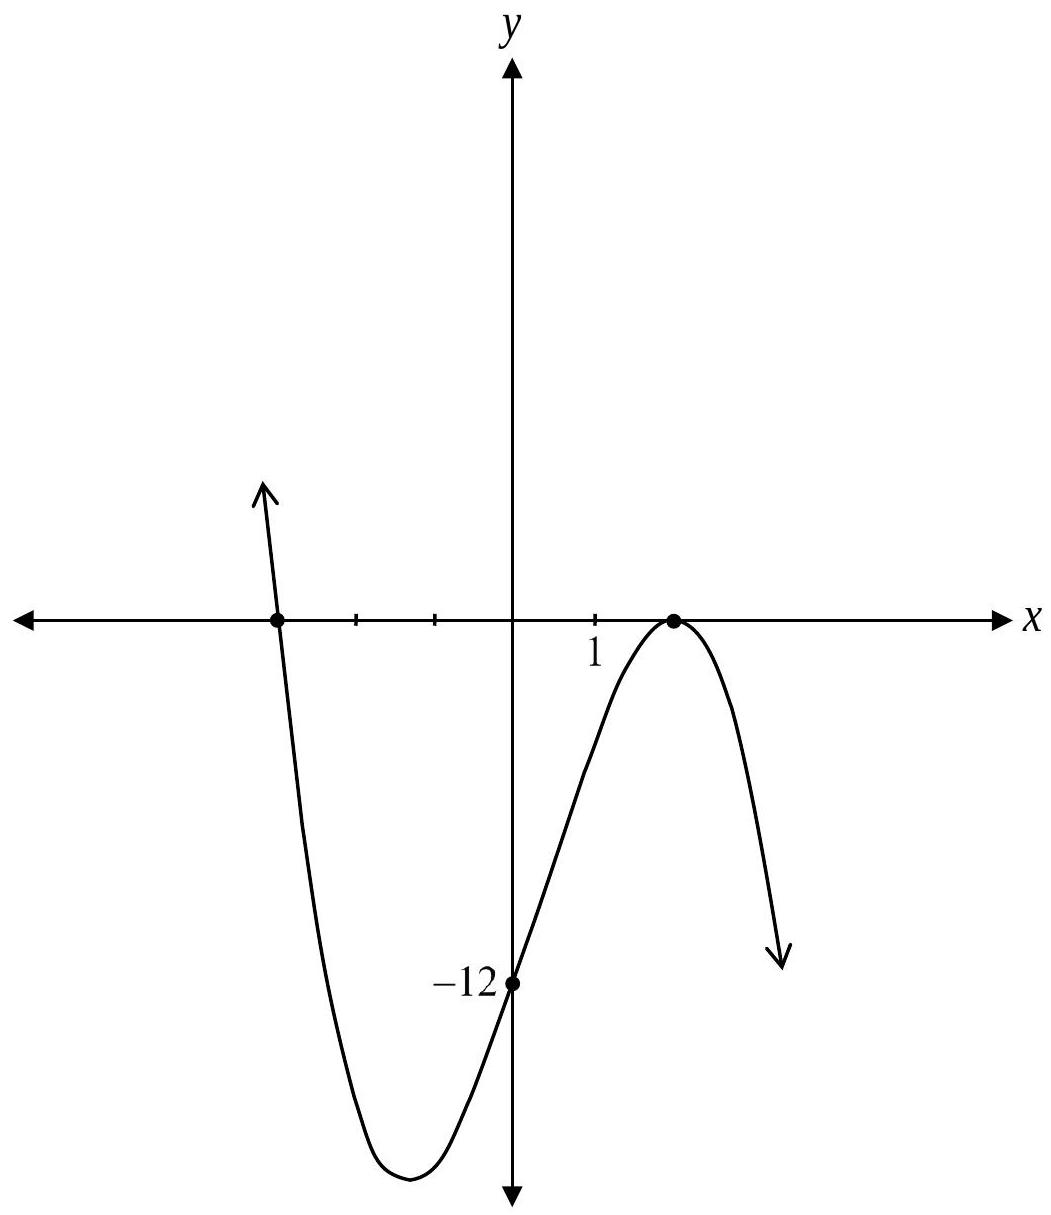
\includegraphics[max width=\textwidth, alt={}]{f67fedaf-ea11-42ad-a16e-f30d2fcf2bd3-316_1215_1051_541_524}
\end{center}

1 mark for $x$-intercepts\\
$\frac{1}{2}$ mark for $y$-intercept\\
1 mark for multiplicity of 2 at $x=2$\\
$\frac{1}{2}$ mark for end behaviour\\
3 marks

Given $f(x)=-2 x-5$ and $g(x)=x+7$, identify the equation of $h(x)=f(g(x))$.\\
a) $h(x)=-2 x^{2}-35$\\
b) $h(x)=-2 x-19$\\
c) $h(x)=-2 x^{2}-19 x-35$\\
d) $h(x)=-2 x+2$

Question 16

The function $y=f(x)$ has a domain of [2,5] and a range of [-6,3]. Identify the range of the function $y=f^{-1}(x)$.\\
a) $[-6,3]$\\
b) $[-5,2]$\\
c) $[-3,6]$\\
d) $[2,5]$

Question 17

Identify the function that has a graph with a point of discontinuity (hole) at $x=-3$.\\
a) $y=\frac{x+3}{x^{2}-9}$\\
b) $y=\frac{x-3}{x^{2}-9}$\\
c) $y=\frac{x^{2}-9}{x-3}$\\
d) $y=\frac{x^{2}+9}{x+3}$

Identify the value of $\ln e$.\\
a) 0\\
b) $\log e$\\
c) 1\\
d) $e$

Question 19

When the polynomial function, $p(x)$, is divided by ( $x-4$ ) the remainder is 17 . Identify which statement is true.\\
a) $p(4)=17$\\
b) $p(-4)=17$\\
c) $p(4)=0$\\
d) $p(-4)=0$

Question 20

Identify the expression equivalent to $\frac{(n-6)!}{(n-4)!}$.\\
a) $(n-4)(n-5)$\\
b) $\frac{1}{(n-4)(n-5)}$\\
c) $(n-6)(n-5)$\\
d) $\frac{1}{(n-6)(n-5)}$

Identify the quadrant in which $\theta$ terminates if $\sec \theta=-\frac{4}{3}$ and $\sin \theta>0$.\\
a) I\\
b) II\\
c) III\\
d) IV

Question 22

Identify the expression that represents all angles that are coterminal with $\frac{\pi}{3}$.\\
a) $\frac{\pi}{3}+\pi k, k \in \mathbb{Z}$\\
b) $\frac{\pi}{3}+\pi k, k \in \mathbb{R}$\\
c) $\frac{\pi}{3}+2 \pi k, k \in \mathbb{Z}$\\
d) $\frac{\pi}{3}+2 \pi k, k \in \mathbb{R}$

Given $f(x)=\frac{1}{2} x-3$, state the coordinates of an invariant (unchanged) point when sketching the graph of $y=\sqrt{f(x)}$.

\section*{Solution}
$$
\begin{aligned}
\frac{1}{2} x-3 & =0 \\
\frac{1}{2} x & =3 \\
x & =6 \\
(6,0) & \text { or } \\
\frac{1}{2} x-3 & =1 \\
\frac{1}{2} x & =4 \\
x & =8 \\
(8,1) &
\end{aligned}
$$

Solve, algebraically.

$$
125^{3 x+4}=\left(\frac{1}{5}\right)^{x}
$$

\section*{Solution}
$\left(5^{3}\right)^{3 x+4}=\left(5^{-1}\right)^{x}$\\
$5^{9 x+12}=5^{-x}$\\
$9 x+12=-x$\\
$10 x=-12$\\
$x=-\frac{12}{10}$\\
or\\
$x=-\frac{6}{5}$

1 mark for changing to a common base ( $\frac{1}{2}$ mark for each side)\\
$\frac{1}{2}$ mark for exponent law\\
$\frac{1}{2}$ mark for equating exponents

\section*{2 marks}
Given $\sin \theta=-\frac{\sqrt{2}}{2}$ and $\cos \theta=-\frac{\sqrt{2}}{2}$, justify that the value of $\tan (2 \theta)$ is undefined.

\section*{Solution}
\section*{Method 1}
$$
\begin{aligned}
\tan (2 \theta) & =\frac{2 \tan \theta}{1-\tan ^{2} \theta} \\
& =\frac{2(1)}{1-1} \\
& =\frac{2}{0}
\end{aligned}
$$

∴ undefined\\
1 mark for value of $\tan \theta$

1 mark for justification

\section*{2 marks}
\section*{Method 2}
$\tan \theta=1$

$$
\begin{aligned}
\theta & =\frac{5 \pi}{4} \\
\tan (2 \theta) & =\tan \left(2\left(\frac{5 \pi}{4}\right)\right) \\
& =\tan \frac{5 \pi}{2}
\end{aligned}
$$

1 mark for value of $\theta$\\
∴ undefined

1 mark for justification\\
2 marks

Sketch the graph of $y=-2 \log _{3} x$.

\section*{Solution}
\begin{center}
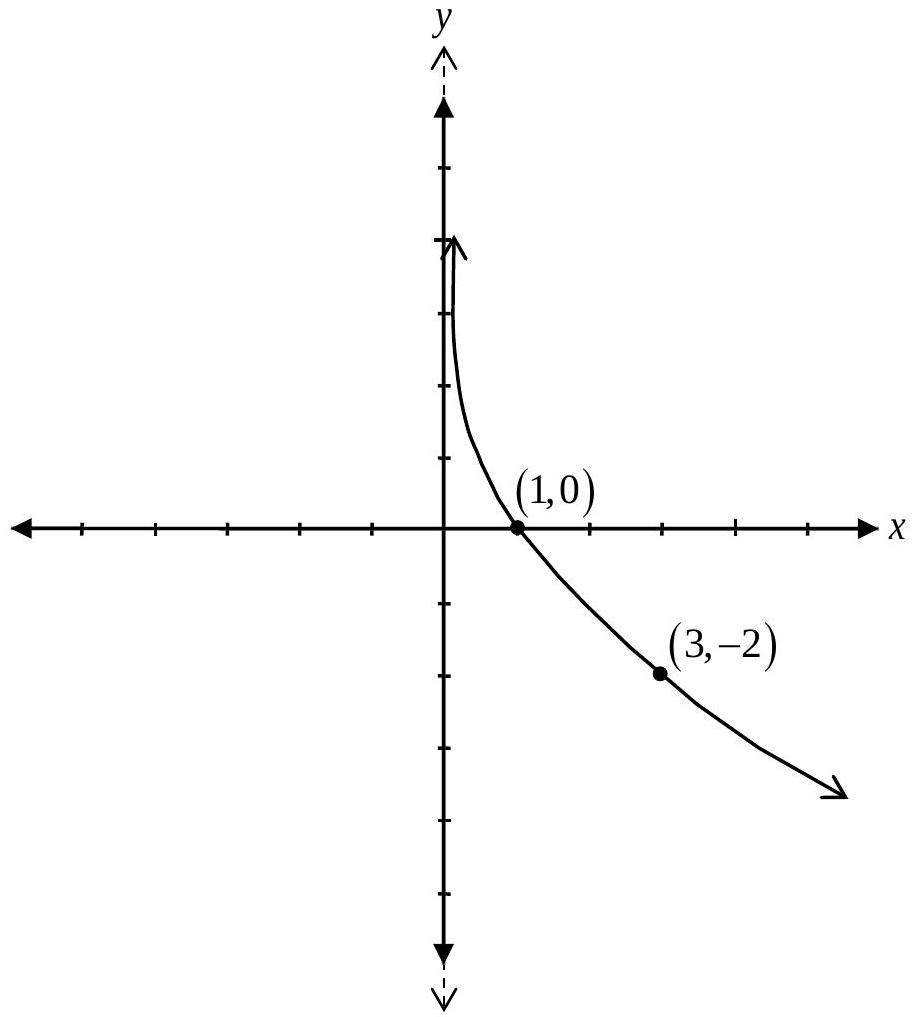
\includegraphics[max width=\textwidth, alt={}]{f67fedaf-ea11-42ad-a16e-f30d2fcf2bd3-323_1017_914_575_249}
\end{center}

1 mark for asymptotic behaviour approaching $x=0$\\
1 mark for vertical reflection\\
1 mark for vertical stretch\\
3 marks

Evaluate.

$$
\cos \left(\pi \cdot \sin \left(-\frac{\pi}{6}\right)\right)
$$

\section*{Solution}
$\cos \left(\pi\left(-\frac{1}{2}\right)\right.$\\
$\cos \left(-\frac{\pi}{2}\right)$\\
0\\
1 mark for consistent value

2 marks\\
a) Given $f(x)=-x+2$, sketch the graph of $h(x)=f(f(x))$.\\
b) Explain why the domain of $h(x)=f(f(x))$ does not have any restrictions.

\section*{Solution}
a)\\
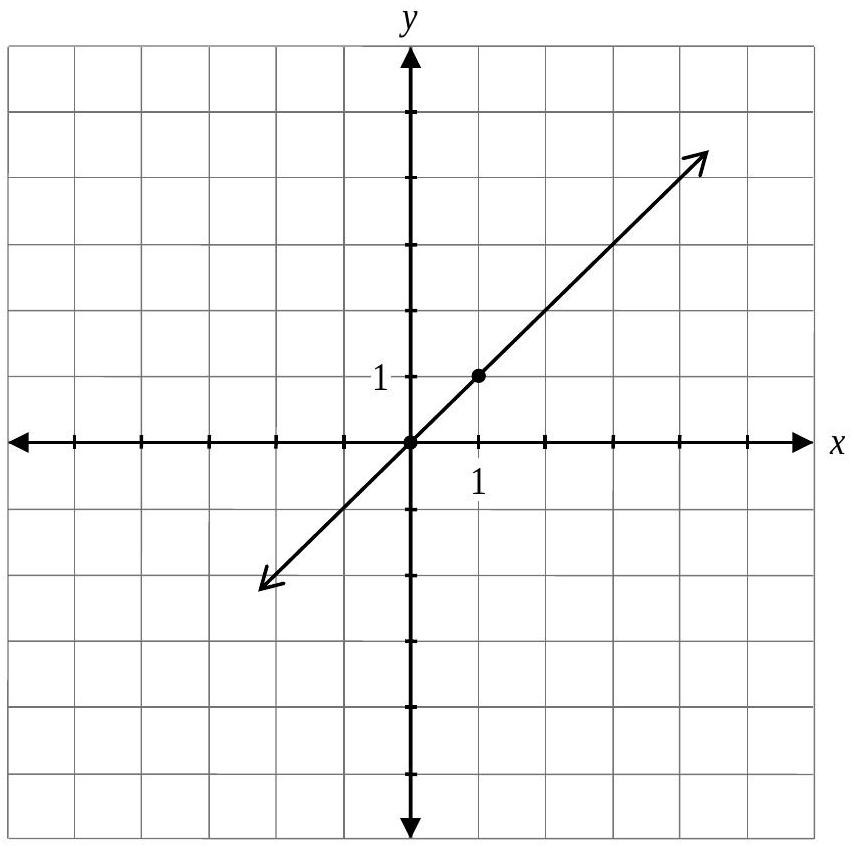
\includegraphics[max width=\textwidth, alt={}, center]{f67fedaf-ea11-42ad-a16e-f30d2fcf2bd3-325_846_854_691_294}\\
b) Since the domain of $y=f(x)$ does not have any restrictions, then the domain of the composition does not have any restrictions.\\
a) Sketch the graph of $f(x)=\frac{3 x-5}{2 x+4}$.\\
b) State the range of $f(x)$.

\section*{Solution}
\begin{center}
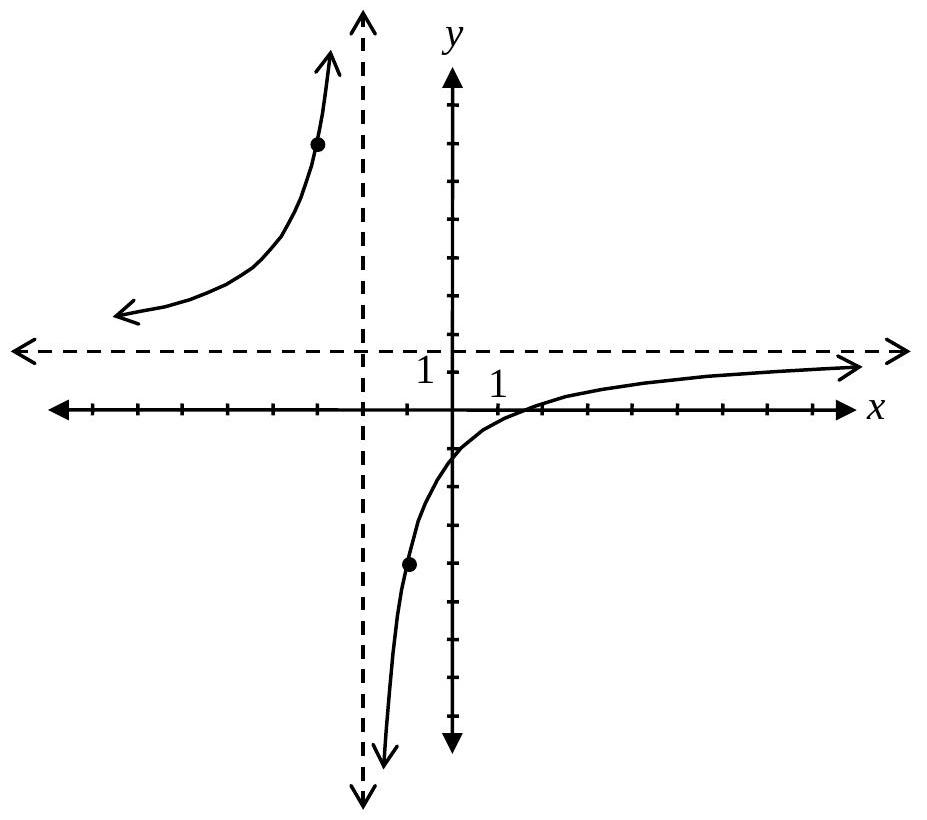
\includegraphics[max width=\textwidth, alt={}]{f67fedaf-ea11-42ad-a16e-f30d2fcf2bd3-326_820_927_809_232}
\end{center}

1 mark for asymptotic behaviour approaching $x=-2$\\
1 mark for asymptotic behaviour approaching $y=\frac{3}{2}$\\
$\frac{1}{2}$ mark for graph right of $x=-2$\\
$\frac{1}{2}$ mark for graph left of $x=-2$\\
3 marks\\
b) Range: $\underline{\left\{y \in \mathbb{R} \left\lvert\, y \neq \frac{3}{2}\right.\right\}}$

1 mark for range consistent with graph\\
□\\
1 mark

Determine, algebraically, the equation of $p(x)$ that satisfies all of the following conditions:

\begin{itemize}
  \item $p(x)$ is a polynomial function of degree 4
  \item $p(x)$ has a zero at 3 with a multiplicity of 2
  \item $p(x)$ has zeroes at -1 and -2
  \item $p(x)$ passes through the point $(2,24)$.
\end{itemize}

\section*{Solution}
$$
\begin{aligned}
p(x) & =a(x+1)(x+2)(x-3)^{2} & & \frac{1}{2} \text { mark for factors of } p(x) \\
24 & =a(2+1)(2+2)(2-3)^{2} & & 1 / 2 \text { mark for multiplicity of } 2 \text { at } x=3 \\
24 & =12 a & & \\
a & =2 & & 1 / 2 \text { mark for consistent value of } a \\
p(x) & =2(x+1)(x+2)(x-3)^{2} & & \mathbf{2} \text { marks }
\end{aligned}
$$

Verify, by substitution, that the equation $\frac{\cos \theta+\cot \theta}{\cot \theta}=1+\sin \theta$ is true for $\theta=\frac{2 \pi}{3}$.

\section*{Solution}
\begin{center}
\begin{tabular}{|l|l|}
\hline
Left-Hand Side & Right-Hand Side \\
\hline
\( \frac{\cos \left(\frac{2 \pi}{3}\right)+\cot \left(\frac{2 \pi}{3}\right)}{\cot \left(\frac{2 \pi}{3}\right)} \) & \( \begin{aligned} & 1+\sin \left(\frac{2 \pi}{3}\right) \quad 1 / 2 \text { mark for substitution } \\ & 1+\frac{\sqrt{3}}{2} \quad 1 \frac{1}{2} \text { marks for exact values }(1 / 2 \text { mark for eack } \end{aligned} \) \\
\hline
$\frac{\frac{-\sqrt{3}-2}{2 \sqrt{3}}}{-\frac{1}{\sqrt{3}}}$ & \begin{tabular}{l}
\( \frac{2+\sqrt{3}}{2} \) \( \frac{\sqrt{3}+2}{2} \) \\
( $\frac{1}{2}$ mark for LHS; $\frac{1}{2}$ mark for RHS) \\
\end{tabular} \\
\hline
\end{tabular}
\end{center}

$\frac{-\sqrt{3}-2}{-2} \frac{-(\sqrt{3}+2)}{-2} \frac{\sqrt{3}+2}{2}$

Note:

\begin{itemize}
  \item Deduct a maximum of 1 mark if student proves identity without substitution of $\theta=\frac{2 \pi}{3}$.
\end{itemize}

\section*{Question 32}
Jyugo was asked to state the equation of the vertical asymptote(s) on the graph of $f(x)=\frac{3 x-15}{x^{2}-5 x}$.

His solution:

$$
\begin{array}{r}
f(x)=\frac{3(x-5)}{x(x-5)} \\
x=0 \quad x=5
\end{array}
$$

Explain why his solution is incorrect.

\section*{Solution}
His solution at $x=5$ is the $x$-value of a point of discontinuity (hole), not a vertical asymptote.

Sketch the graph of $y=\sin \left(\frac{1}{2} x\right)-1$ over the interval $[-2 \pi, 2 \pi]$.

\section*{Solution}
\begin{center}
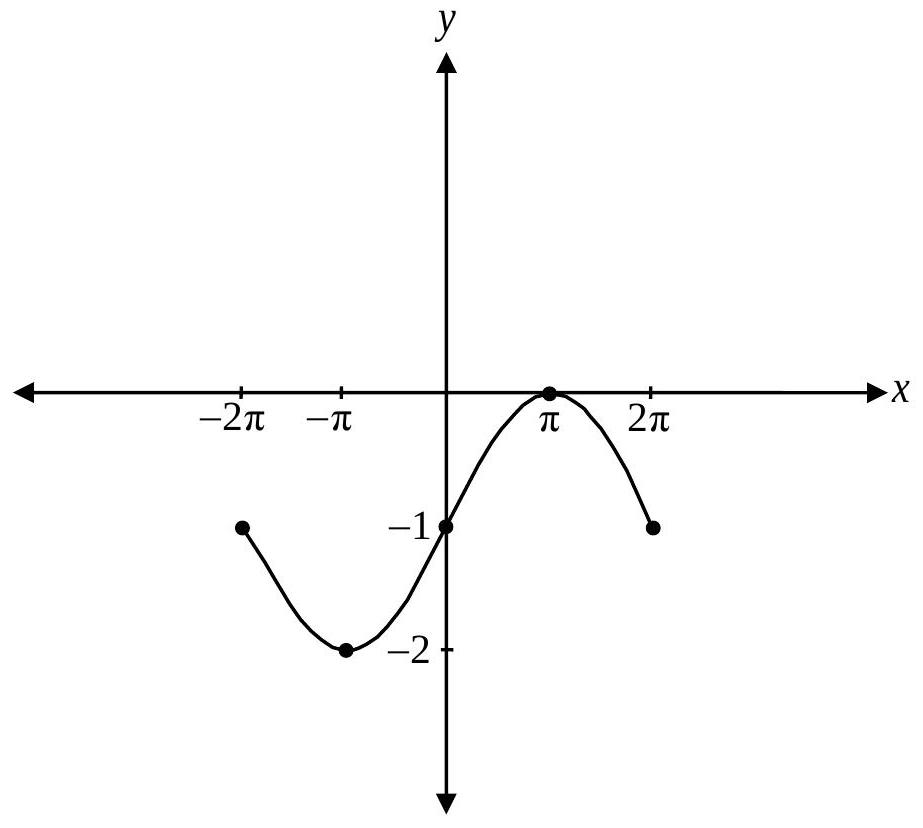
\includegraphics[max width=\textwidth, alt={}]{f67fedaf-ea11-42ad-a16e-f30d2fcf2bd3-330_828_923_672_244}
\end{center}

1 mark for shape of $y=\sin x$\\
1 mark for period\\
1 mark for vertical translation

3 marks

Sketch the graph of $y=\sqrt{-2 x+6}$.

\section*{Solution}
\begin{center}
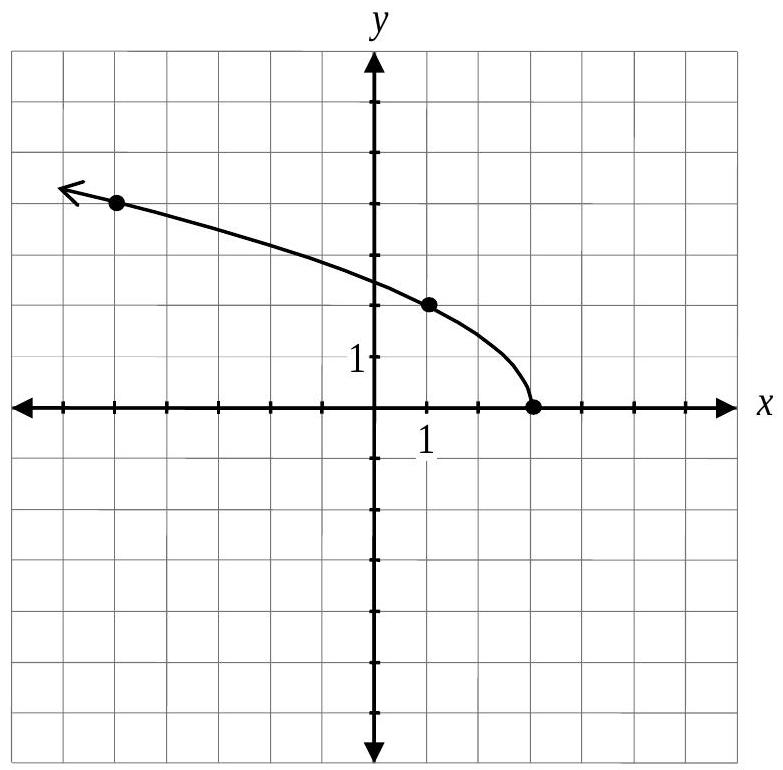
\includegraphics[max width=\textwidth, alt={}]{f67fedaf-ea11-42ad-a16e-f30d2fcf2bd3-331_770_783_558_247}
\end{center}

1 mark for shape of a radical function 1 mark for horizontal reflection 1 mark for horizontal compression 1 mark for horizontal translation

Determine the measure of angle R , in radians.\\
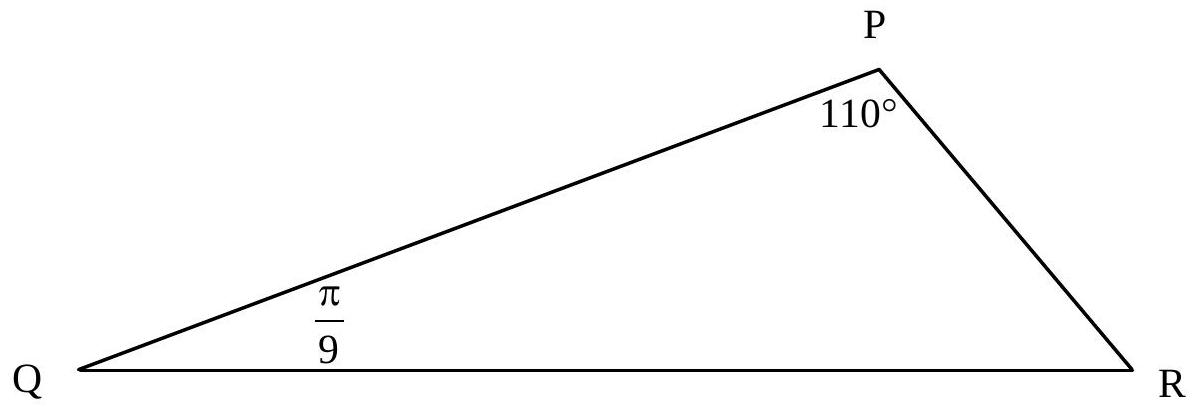
\includegraphics[max width=\textwidth, alt={}, center]{f67fedaf-ea11-42ad-a16e-f30d2fcf2bd3-332_411_1198_451_442}

\section*{Solution}
$(110)\left(\frac{\pi}{180}\right)=\frac{11 \pi}{18}$\\
1 mark for conversion\\
$\angle \mathrm{R}=\pi-\left(\frac{\pi}{9}+\frac{11 \pi}{18}\right)$\\
$\angle \mathrm{R}=\frac{18 \pi}{18}-\left(\frac{2 \pi}{18}+\frac{11 \pi}{18}\right)$\\
$\angle \mathrm{R}=\frac{5 \pi}{18}$\\
1 mark for angle R\\
2 marks

Given $f(x)=\sqrt{x-4}$, state the equation of the resulting function, $g(x)$, after a reflection over the $x$-axis.

\section*{Solution}
$$
\begin{array}{lc}
g(x)=-\sqrt{x-4} & 1 \text { mark for vertical reflection } \\
\mathbf{1} \text { mark }
\end{array}
$$

a) Determine the coterminal angle of $\frac{29 \pi}{12}$ over the interval $[0,2 \pi]$.\\
b) Determine the exact value of $\sin \left(\frac{29 \pi}{12}\right)$.

\section*{Solution}
a) $\frac{5 \pi}{12} \quad \mathbf{1}$ mark\\
b)

$$
\begin{aligned}
\sin \left(\frac{5 \pi}{12}\right) & =\sin \left(\frac{\pi}{6}+\frac{\pi}{4}\right) \\
& =\sin \frac{\pi}{6} \cos \frac{\pi}{4}+\cos \frac{\pi}{6} \sin \frac{\pi}{4} \\
& =\left(\frac{1}{2}\right)\left(\frac{\sqrt{2}}{2}\right)+\left(\frac{\sqrt{3}}{2}\right)\left(\frac{\sqrt{2}}{2}\right) \\
& =\frac{\sqrt{2}}{4}+\frac{\sqrt{6}}{4} \\
& =\frac{\sqrt{2}+\sqrt{6}}{4}
\end{aligned}
$$

or

$$
=\frac{1+\sqrt{3}}{2 \sqrt{2}}
$$

1 mark for substitution into correct identity

2 marks ( $\frac{1}{2}$ mark for each exact value)

3 marks

Note:

\begin{itemize}
  \item Other combinations are possible.
\end{itemize}

Given the graphs of $f(x)$ and $g(x)$, sketch the graph of $h(x)=f(x)-g(x)$.\\
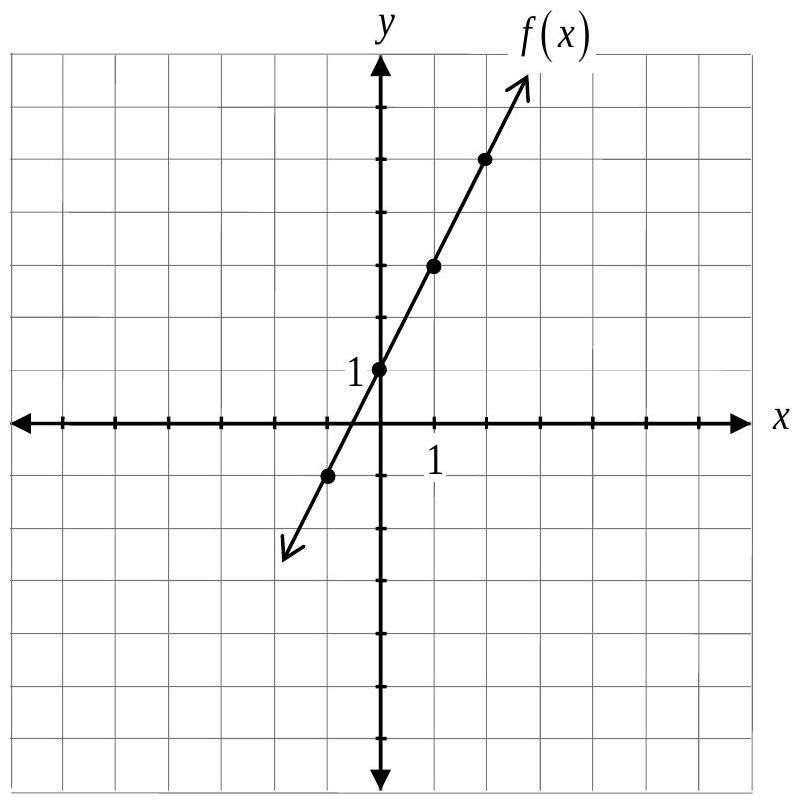
\includegraphics[max width=\textwidth, alt={}, center]{f67fedaf-ea11-42ad-a16e-f30d2fcf2bd3-335_803_798_489_249}\\
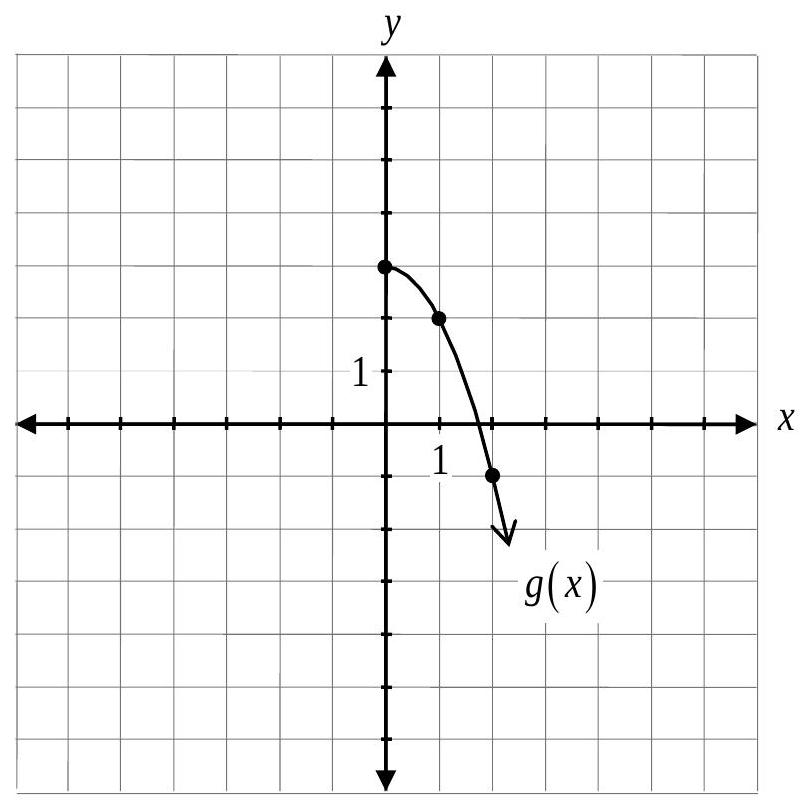
\includegraphics[max width=\textwidth, alt={}, center]{f67fedaf-ea11-42ad-a16e-f30d2fcf2bd3-335_805_811_487_1074}

\section*{Solution}
\begin{center}
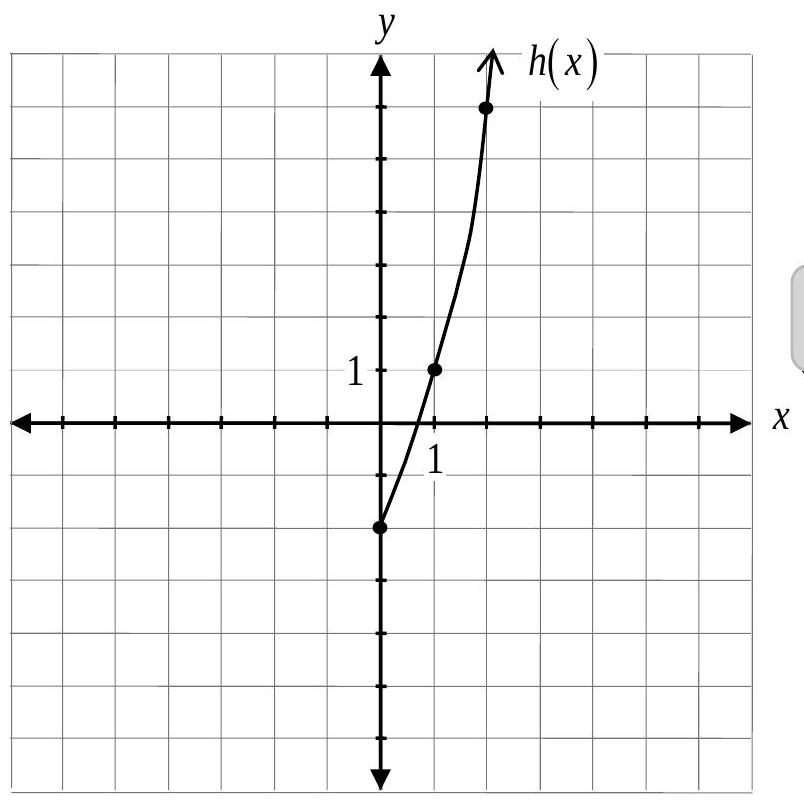
\includegraphics[max width=\textwidth, alt={}]{f67fedaf-ea11-42ad-a16e-f30d2fcf2bd3-335_804_804_1452_249}
\end{center}

1 mark for operation of subtraction\\
1 mark for restricted domain\\
2 marks

Determine an equation of a sinusoidal function that has the following characteristics:

\begin{itemize}
  \item an amplitude of 3
  \item a period of 6
  \item a minimum value of -5
\end{itemize}

\section*{Solution}
$$
\left.\begin{array}{ll}
y=A \sin (B x)+D & \\
y=3 \sin \left(\frac{\pi}{3} x\right)-2 & \begin{array}{l}
1 \text { mark for value of } \mathrm{A} \\
1 \text { mark for value of } \mathrm{B}
\end{array} \\
\text { or } & 3 \text { mark for value of } \mathrm{D}
\end{array}\right\} \begin{array}{ll}
\mathbf{3} \text { marks } \\
y=A \cos (B x)+D & \\
y=3 \cos \left(\frac{\pi}{3} x\right)-2 &
\end{array}
$$

Note:

\begin{itemize}
  \item Other equations are possible.
\end{itemize}

Given the graph of $y=f(x)$, sketch the graph after a reflection over the line $y=x$.

\section*{Solution}
\begin{center}
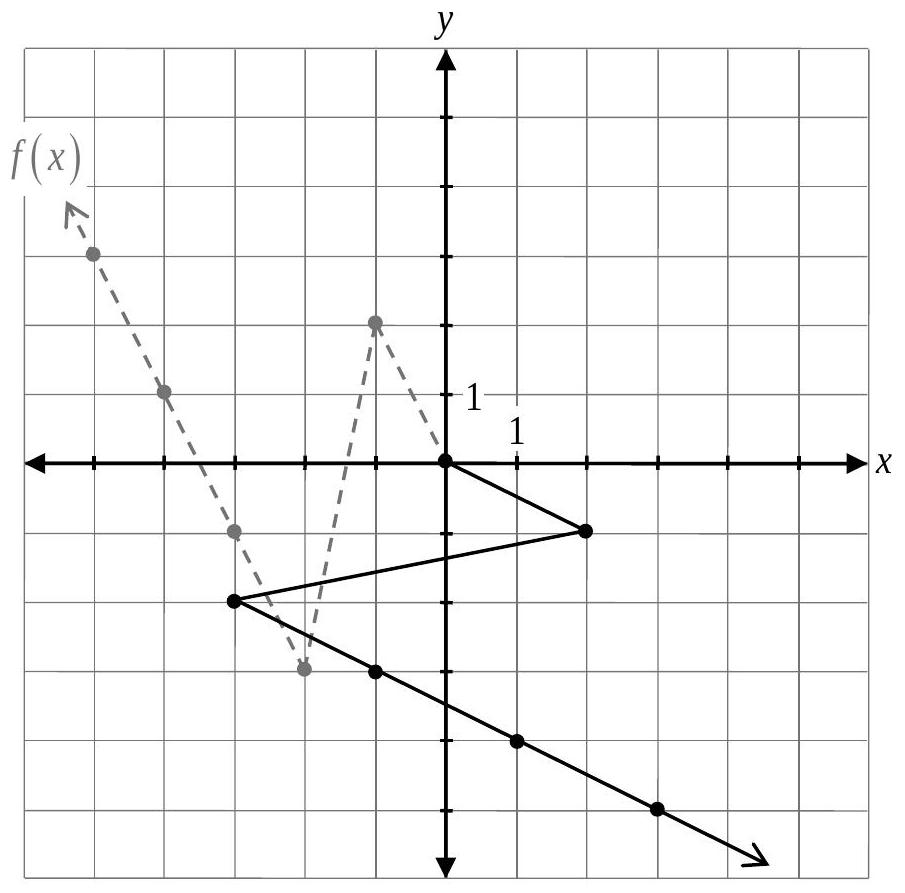
\includegraphics[max width=\textwidth, alt={}]{f67fedaf-ea11-42ad-a16e-f30d2fcf2bd3-337_893_905_588_236}
\end{center}

1 mark for reflection over the line $y=x$ 1 mark\\
a) Determine the remainder when $3 x^{3}+5 x^{2}-13 x-3$ is divided by $(x+3)$.\\
b) Is $(x+3)$ a factor of $3 x^{3}+5 x^{2}-13 x-3$ ? Explain your reasoning.

\section*{Solution}
a) $3(-3)^{3}+5(-3)^{2}-13(-3)-3$ 1 mark for remainder theorem

$$
3(-27)+5(9)-13(-3)-3
$$

0\\
or

\begin{center}
\begin{tabular}{r|rrrr}
-3 & 3 & 5 & -13 & -3 \\
 &  & -9 & 12 & 3 \\
\hline
 & 3 & -4 & -1 & 0 \\
\hline
\end{tabular}
\end{center}

1 mark for synthetic division (or any equivalent strategy)

The remainder is 0 .\\
b) Yes, because the remainder is 0 .\\
□\\
1 mark

1 mark for explanation\\
□\\
1 mark

State the range, the $y$-intercept, and the equation of the asymptote of the exponential function, $f(x)=3^{x-1}+2$.

\section*{Solution}
Range: $(2, \infty) \quad 1$ mark for range\\
$y$-intercept: $\underline{\frac{7}{3}} \quad 1$ mark for $y$-intercept\\
Equation of the asymptote: $y=2 \quad 1$ mark for equation of the asymptote\\
3 marks

The graph of $y=2 \cos (3 x)-1$ below can be used to solve the equation $0=2 \cos (3 x)-1$ over the interval $[0,2 \pi]$. Indicate on the graph where to find at least one solution to the equation $0=2 \cos (3 x)-1$.\\
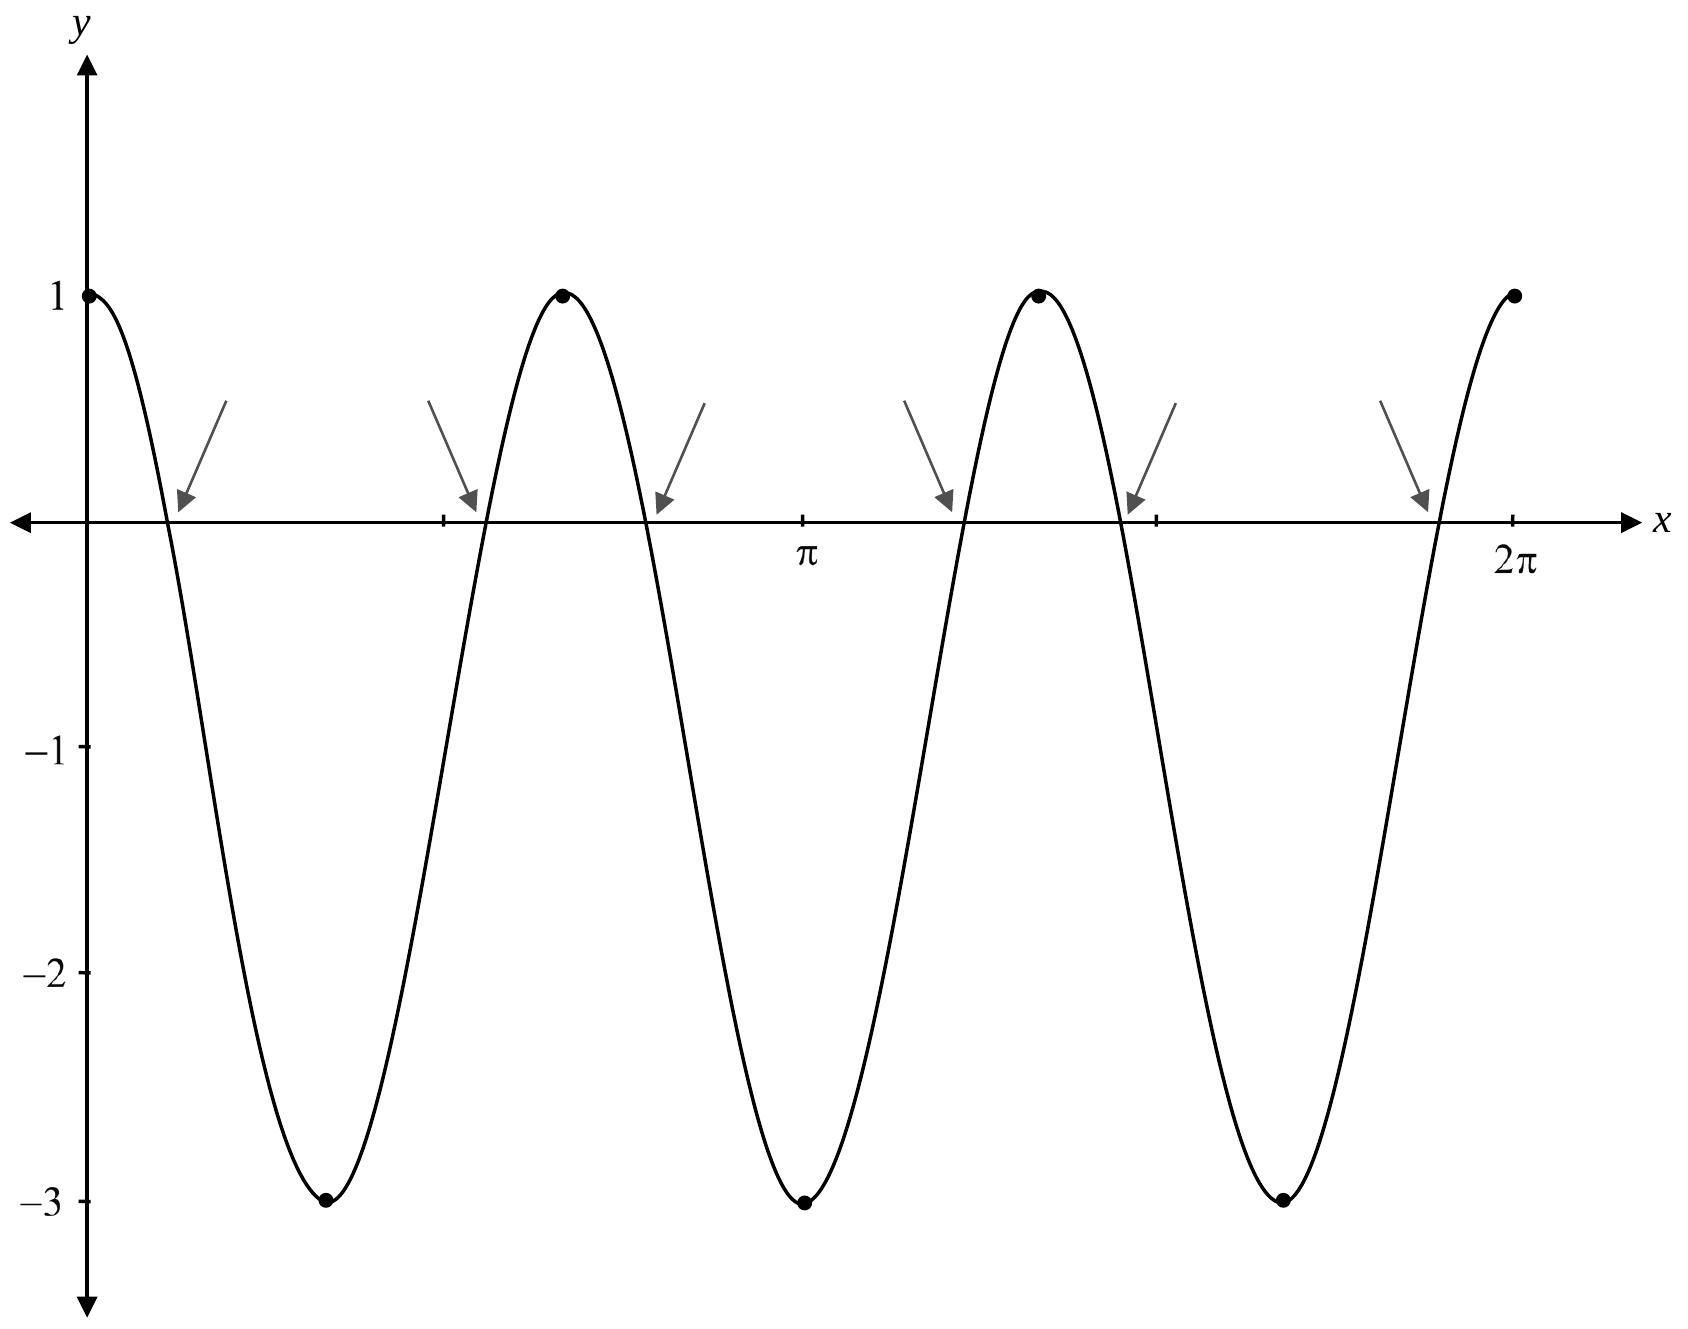
\includegraphics[max width=\textwidth, alt={}, center]{f67fedaf-ea11-42ad-a16e-f30d2fcf2bd3-340_1329_1688_592_240}

\section*{Solution}
See arrows on graph above. 1 mark for indicating a solution on graph

\section*{1 mark}
Note:

\begin{itemize}
  \item Students do not need to show all six arrows.
\end{itemize}

A pendulum that is 35 cm long swings through an angle of $50^{\circ}$. Determine the length of the arc through which the pendulum swings.\\
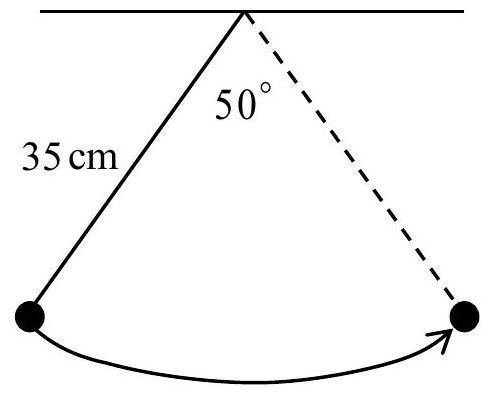
\includegraphics[max width=\textwidth, alt={}, center]{f67fedaf-ea11-42ad-a16e-f30d2fcf2bd3-341_394_493_550_782}

\section*{Solution}
$$
\begin{aligned}
\theta & =50\left(\frac{\pi}{180}\right) \\
& =\frac{5 \pi}{18} \\
& \text { or } \\
& =0.872664 \ldots
\end{aligned}
$$

$$
\begin{array}{rlr}
s & =\theta r \\
& =\left(\frac{5 \pi}{18}\right)(35) & 1 \text { mark for substitution } \\
& =\frac{175 \pi}{18} \mathrm{~cm} & \mathbf{2} \text { marks }
\end{array}
$$

or\\
$=30.543 \mathrm{~cm}$

Solve algebraically, where $0 \leq \theta \leq 2 \pi$.

$$
2 \cos ^{2} \theta=\sin ^{2} \theta-2 \cos \theta
$$

\section*{Solution}
$2 \cos ^{2} \theta=1-\cos ^{2} \theta-2 \cos \theta$\\
$3 \cos ^{2} \theta+2 \cos \theta-1=0$\\
$(\cos \theta+1)(3 \cos \theta-1)=0$\\
$\cos \theta=-1 \quad \cos \theta=\frac{1}{3}$\\
$\theta=\pi$\\
$\theta_{r}=1.230959 \ldots$\\
$\theta=1.231,5.052$

1 mark for substitution of appropriate identity

1 mark for solving for $\cos \theta$

2 marks for solving for $\theta$ ( 1 mark for each branch)\\
4 marks

Determine the number of arrangements of the letters in the word ATTENTION which begin with the letter A.

\section*{Solution}
$$
\frac{8!}{3!2!}=3360
$$

1 mark for 8 !\\
1 mark for division by $3!2!\left(\frac{1}{2}\right.$ mark for $3!; 1 / 2$ mark for $\left.2!\right)$

\section*{2 marks}
Solve for $x$, algebraically.

$$
e^{2 x+1}=5^{x}
$$

\section*{Solution}
$$
\begin{aligned}
\ln \left(e^{2 x+1}\right) & =\ln \left(5^{x}\right) & & 1 / 2 \text { mark for applying logarithms } \\
(2 x+1) \ln e & =x \ln 5 & & 1 \text { mark for power law }(1 / 2 \text { mark for each }) \\
2 x+1 & =x \ln 5 & & \\
2 x-x \ln 5 & =-1 & & 1 / 2 \text { mark for collecting terms with } x \\
x(2-\ln 5) & =-1 & & \\
x & =\frac{-1}{2-\ln 5} & & 1 / 2 \text { mark for isolating } x \\
x & =-2.560 \quad 412 \ldots & & \\
x & =-2.560 & & 1 / 2 \text { mark for evaluating quotient of logarithms }
\end{aligned}
$$

There are 10 teachers and 17 students who would like to attend a field trip.\\
Determine the number of ways that 3 teachers and 9 students can be selected given that Mr. Jones and Mrs. Carol, two of the teachers, must be selected to attend the field trip.

\section*{Solution}
${ }_{2} C_{2} \cdot{ }_{8} C_{1} \cdot{ }_{17} C_{9}$\\
194480\\
1 mark for ${ }_{8} C_{1}$\\
$\frac{1}{2}$ mark for ${ }_{17} C_{9}$\\
$\frac{1}{2}$ mark for product of combinations\\
2 marks

Note:

\begin{itemize}
  \item ${ }_{2} C_{2}$ does not need to be shown.
\end{itemize}

Given the graph of $f(x)$, sketch the graph of $y=-f(2 x)$.

\section*{Solution}
\begin{center}
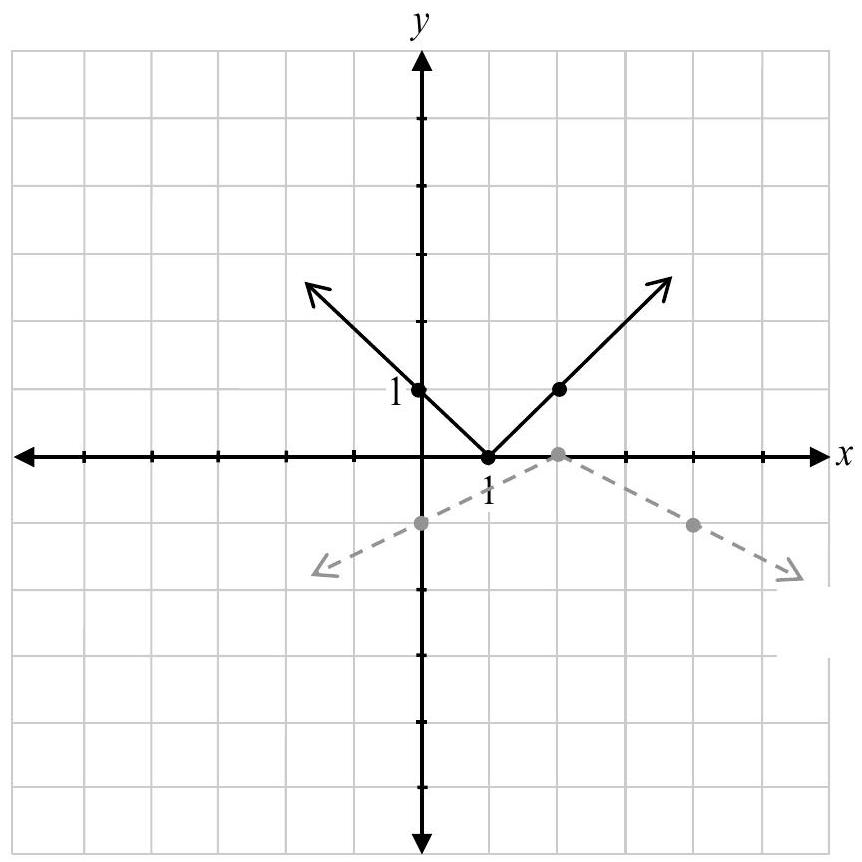
\includegraphics[max width=\textwidth, alt={}]{f67fedaf-ea11-42ad-a16e-f30d2fcf2bd3-346_862_862_580_249}
\end{center}

1 mark for vertical reflection 1 mark for horizontal compression

2 marks

There are 5 roads between Anneville and Berrybourg, and 2 roads between Berrybourg and Carriton.

Determine how many ways Blake can travel from Anneville to Carriton and back to Anneville, given the following conditions:

\begin{itemize}
  \item he must travel through Berrybourg in both directions
  \item he cannot use the same road twice
\end{itemize}

\section*{Solution}
$\underline{5}$ - 2

Determine which term contains $x^{0}$ in the binomial expansion of $\left(x^{2}+\frac{1}{x}\right)^{6}$.

\section*{Solution}
\section*{Method 1}
$$
\begin{aligned}
x^{0} & =\left(x^{2}\right)^{6-k}\left(\frac{1}{x}\right)^{k} \\
x^{0} & =x^{12-2 k} x^{-k} \\
x^{0} & =x^{12-3 k} \\
3 k & =12 \\
k & =4
\end{aligned}
$$

∴ the fifth term\\
$\frac{1}{2}$ mark for substitution\\
$\frac{1}{2}$ mark for solving for $k$\\
1 mark for the fifth term (or a term consistent with the value of $k$ )

\section*{2 marks}
\section*{Method 2}
$\left(x^{2}\right)^{6},\left(x^{2}\right)^{5}\left(\frac{1}{x}\right),\left(x^{2}\right)^{4}\left(\frac{1}{x}\right)^{2} \quad 1$ mark for determining the pattern\\
$x^{12}, x^{9}, x^{6} \ldots$\\
∴ the fifth term\\
1 mark for the fifth term (or a term consistent with the pattern)

Given $f(x)=x^{3}+1$, determine the equation of $f^{-1}(x)$.

\section*{Solution}
Let $y=f(x)$\\
$y=x^{3}+1$\\
To determine the inverse of $f(x)$, switch $x$ and $y$.\\
$x=y^{3}+1$\\
1 mark for switching $x$ and $y$\\
$x-1=y^{3}$\\
$\sqrt[3]{x-1}=y$\\
$\frac{1}{2}$ mark for isolating $y$\\
$f^{-1}(x)=\sqrt[3]{x-1}$\\
$\frac{1}{2}$ mark for writing equation in terms of $f^{-1}(x)$\\
2 marks

Guillermo was asked to determine the number of ways to select a president, a vice president, and a treasurer from a group of 11 people.

His solution: ${ }_{11} C_{3}$.\\
Explain why he should have used a permutation instead of a combination.

\section*{Solution}
He should have used a permutation because the people are being selected for specific positions.

Prove the following identity for all permissible values of $x$.

$$
\frac{\csc ^{2} x \sec x}{\tan x+\cot x}=\csc x
$$

\section*{Solution}
\begin{center}
\begin{tabular}{|l|l|}
\hline
Left-Hand Side & Right-Hand Side \\
\hline
\( \begin{gathered} \frac{\left(\frac{1}{\sin ^{2} x}\right)\left(\frac{1}{\cos x}\right)}{\frac{\sin x}{\cos x}+\frac{\cos x}{\sin x}} \\ \frac{1}{\frac{\sin ^{2} x \cos x}{\sin ^{2} x+\cos ^{2} x}} \\ \frac{\sin x \cos x}{\sin ^{2} x \cos x} \cdot \frac{\sin x \cos x}{1} \\ \frac{1}{\sin x} \\ \csc x \end{gathered} \) & $\csc x$ \\
\hline
\end{tabular}
\end{center}

1 mark for correct substitution of identities\\
1 mark for algebraic strategies\\
1 mark for logical process to prove the identity\\
□\\
3 marks

Determine the value of $x$, algebraically.

$$
5 \log _{a} 2-\frac{1}{4} \log _{a} 16=\log _{a} x
$$

\section*{Solution}
$$
\begin{aligned}
\log _{a} 2^{5}-\log _{a} 16^{\frac{1}{4}} & =\log _{a} x \\
\log _{a}\left(\frac{32}{2}\right) & =\log _{a} x \\
\log _{a} 16 & =\log _{a} x \\
x & =16
\end{aligned}
$$

1 mark for power law ( $\frac{1}{2}$ mark for each)\\
1 mark for quotient law

1 mark for equating arguments

Tamara must determine the factors of $x^{4}-13 x+2 x^{3}-14 x^{2}+24$.\\
Explain why the coefficients Tamara used to set up her synthetic division are not written correctly.\\
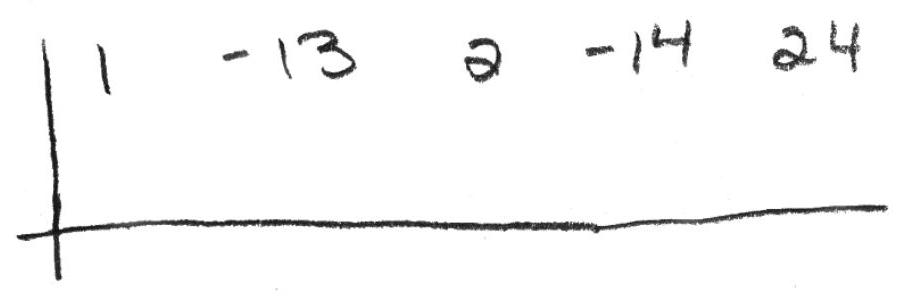
\includegraphics[max width=\textwidth, alt={}, center]{f67fedaf-ea11-42ad-a16e-f30d2fcf2bd3-353_296_903_648_571}

\section*{Solution}
Tamara did not arrange the coefficients of the terms in order of descending degree.\\

\includegraphics[max width=\textwidth, alt={}, center]{f67fedaf-ea11-42ad-a16e-f30d2fcf2bd3-353_130_218_1153_928}

Determine the equation of the graph of $g(x)$ in terms of $f(x)$.\\
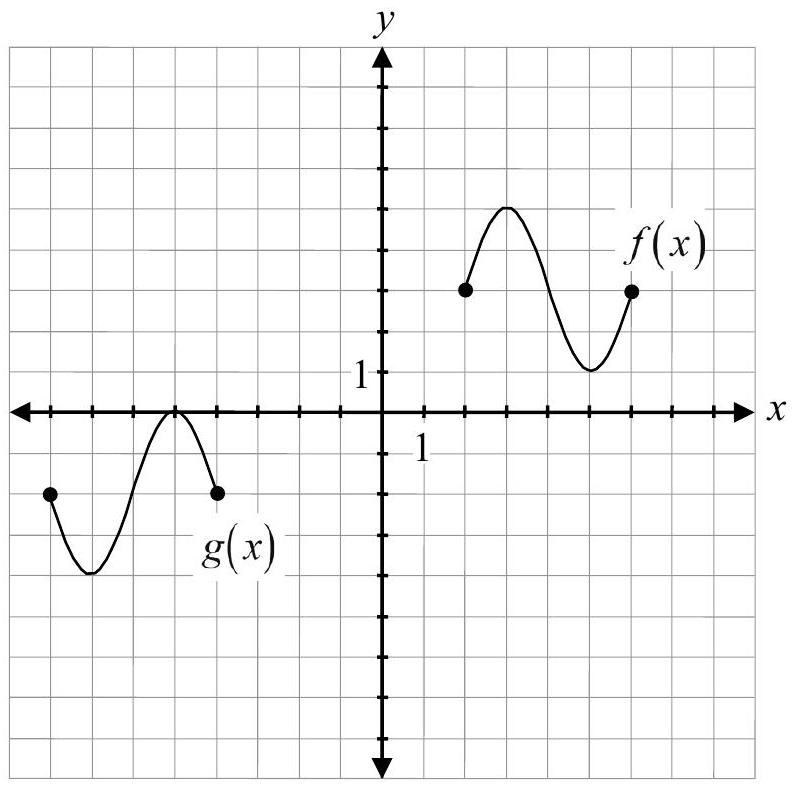
\includegraphics[max width=\textwidth, alt={}, center]{f67fedaf-ea11-42ad-a16e-f30d2fcf2bd3-354_789_798_537_653}

\section*{Solution}
$g(x)=f(-(x+2))-5$\\
or\\
$g(x)=-f(x+10)+1$

1 mark for horizontal reflection\\
1 mark for horizontal translation\\
1 mark for vertical translation

1 mark for vertical reflection\\
1 mark for horizontal translation 1 mark for vertical translation

3 marks

Expand, using the laws of logarithms.

$$
\log _{2}\left[\frac{(x-1)(x-2)}{x}\right]
$$

\section*{Solution}
$$
\log _{2}(x-1)+\log _{2}(x-2)-\log _{2} x \quad 1 \text { mark for product law }
$$

Identify the range of the function $g(x)=\frac{1}{2} f(x+1)$, given that the range of the function $y=f(x)$ is $[-6,4]$.\\
a) $[-12,8]$\\
b) $[-7,3]$\\
c) $[-5,5]$\\
d) $[-3,2]$

Question 17\\
P4

Identify the value of $a$, given that there are 11 terms in the expansion of $\left(3 x^{4}-y\right)^{2 a}$.\\
a) 5\\
b) 6\\
c) 10\\
d) 11

Identify the angle that best represents $\theta=-\frac{6 \pi}{5}$.

\begin{figure}[h]
\begin{center}
\captionsetup{labelformat=empty}
\caption{a)}
  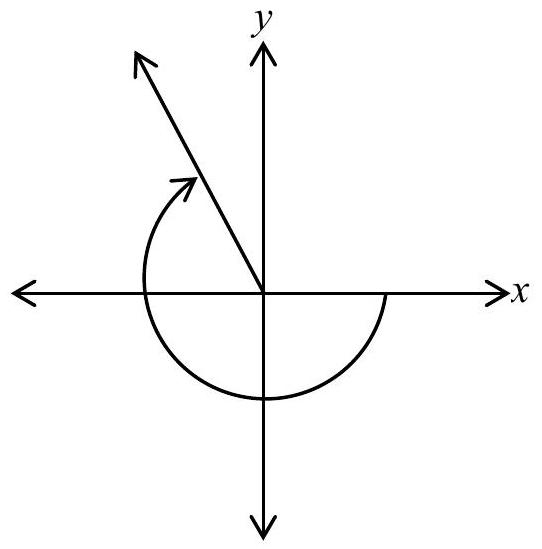
\includegraphics[alt={},max width=\textwidth]{f67fedaf-ea11-42ad-a16e-f30d2fcf2bd3-357_549_542_526_322}
\end{center}
\end{figure}

\begin{center}
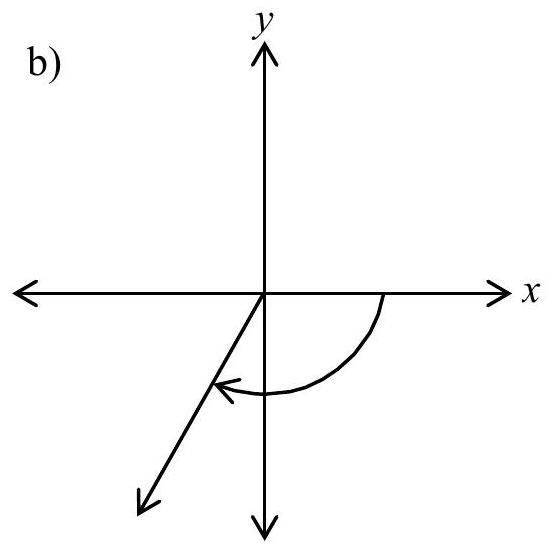
\includegraphics[max width=\textwidth, alt={}]{f67fedaf-ea11-42ad-a16e-f30d2fcf2bd3-357_553_555_522_1222}
\end{center}

\begin{figure}[h]
\begin{center}
\captionsetup{labelformat=empty}
\caption{c)}
  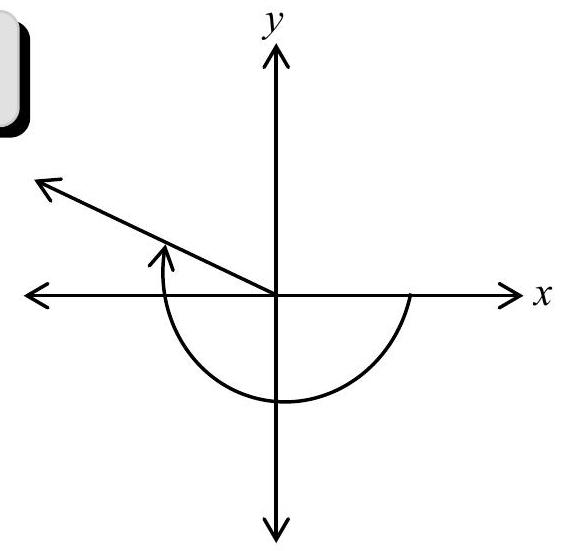
\includegraphics[alt={},max width=\textwidth]{f67fedaf-ea11-42ad-a16e-f30d2fcf2bd3-357_551_562_1250_309}
\end{center}
\end{figure}

\begin{center}
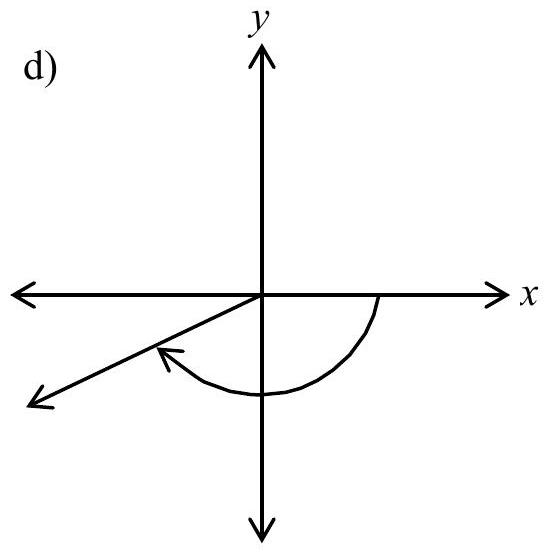
\includegraphics[max width=\textwidth, alt={}]{f67fedaf-ea11-42ad-a16e-f30d2fcf2bd3-357_553_549_1250_1224}
\end{center}

Identify a possible value for $n$, given the graph of $y=-\frac{1}{2}(x+2)^{2}(x-1)^{n}$.\\
a) 1\\
b) 2\\
c) 3\\
d) 4\\
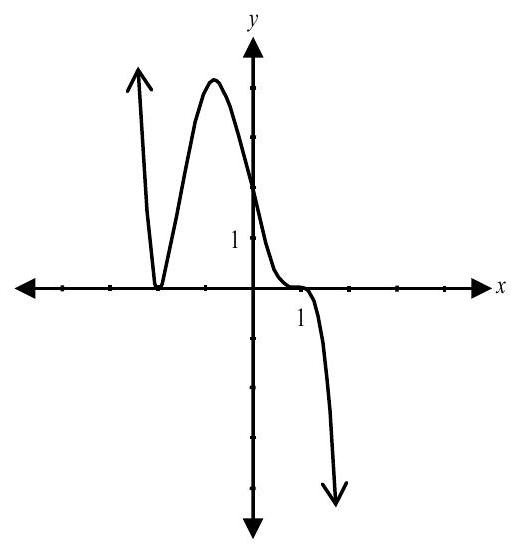
\includegraphics[max width=\textwidth, alt={}, center]{f67fedaf-ea11-42ad-a16e-f30d2fcf2bd3-358_549_519_472_777}

Question 20

Identify the statement that is false, given $g(x)=\frac{8 x^{2}}{x^{2}-16}$.\\
a) the graph of $g(x)$ has one $x$-intercept.\\
b) the graph of $g(x)$ has a point of discontinuity (hole) at $x=0$.\\
c) the graph of $g(x)$ has two vertical asymptotes.\\
d) the graph of $g(x)$ has a horizontal asymptote at $y=8$.

Question 21

Identify the equivalent form of $\log _{a}\left(\frac{1}{x^{2}}\right)$.\\
a) $-2 \log _{a} x$\\
b) $1-2 \log _{a} x$\\
c) $2 \log _{a} x$\\
d) $-2 \log _{a}\left(\frac{1}{x}\right)$

Identify which one of the following expressions is equivalent to ${ }_{13} C_{6}$.\\
a) ${ }_{13} P_{6}$\\
b) ${ }_{13} C_{7}$\\
c) ${ }_{12} P_{7}$\\
d) ${ }_{12} C_{6}$

Question 23

Identify the equation of $h(x)=f(x)-g(x)$, given $f(x)=x+5$ and $g(x)=4 x+1$.\\
a) $h(x)=-3 x+6$\\
b) $h(x)=-3 x+4$\\
c) $h(x)=3 x+6$\\
d) $h(x)=3 x-4$

Determine the equation of the radical function represented by the graph.\\
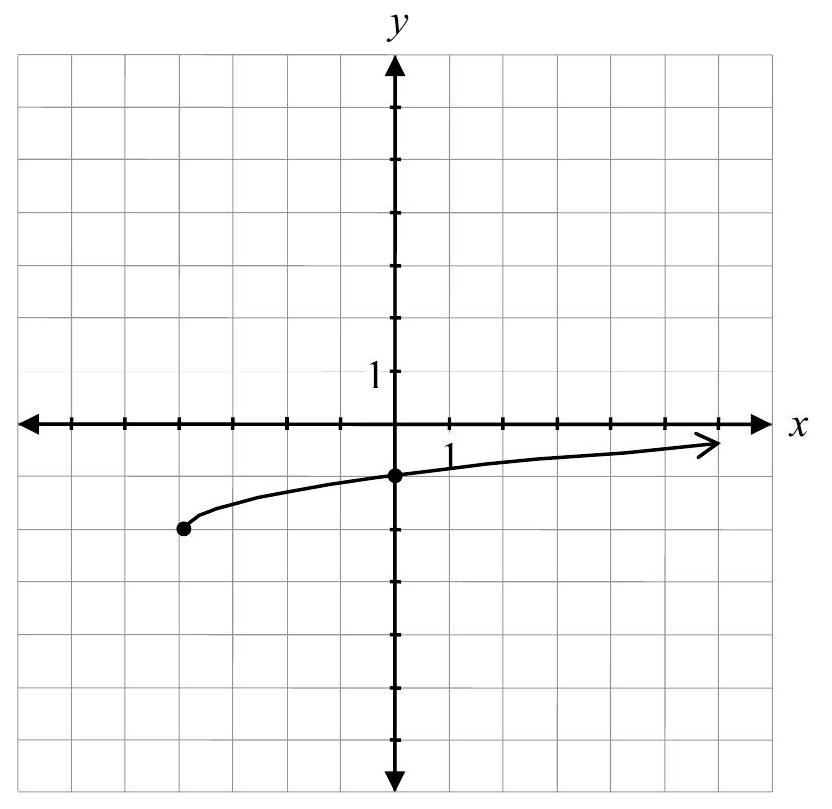
\includegraphics[max width=\textwidth, alt={}, center]{f67fedaf-ea11-42ad-a16e-f30d2fcf2bd3-360_809_832_466_623}

\section*{Solution}
$y=\frac{1}{2} \sqrt{x+4}-2$\\
1 mark for vertical compression\\
1 mark for horizontal translation\\
1 mark for vertical translation\\
3 marks\\
or\\
$y=\sqrt{\frac{1}{4}(x+4)}-2$

1 mark for horizontal stretch\\
1 mark for horizontal translation\\
1 mark for vertical translation

3 marks

Determine the exact value of $x$.

$$
\sec \left(\frac{2 \pi}{3}\right)\left(\sin \left(-\frac{5 \pi}{3}\right)\right)(x)=3
$$

\section*{Solution}
$(-2)\left(\frac{\sqrt{3}}{2}\right)(x)=3$

$$
\begin{aligned}
-\sqrt{3}(x) & =3 \\
x & =-\frac{3}{\sqrt{3}}
\end{aligned}
$$

or

$$
x=-\sqrt{3}
$$

1 mark for $\sec \left(\frac{2 \pi}{3}\right)\left(\frac{1}{2}\right.$ mark for value; $1 / 2$ mark for quadrant)\\
1 mark for $\sin \left(-\frac{5 \pi}{3}\right)\left(\frac{1}{2}\right.$ mark for value; $\frac{1}{2}$ mark for quadrant)\\
2 marks

Sketch the graph of $y=2^{-x}-3$.

\section*{Solution}
\begin{center}
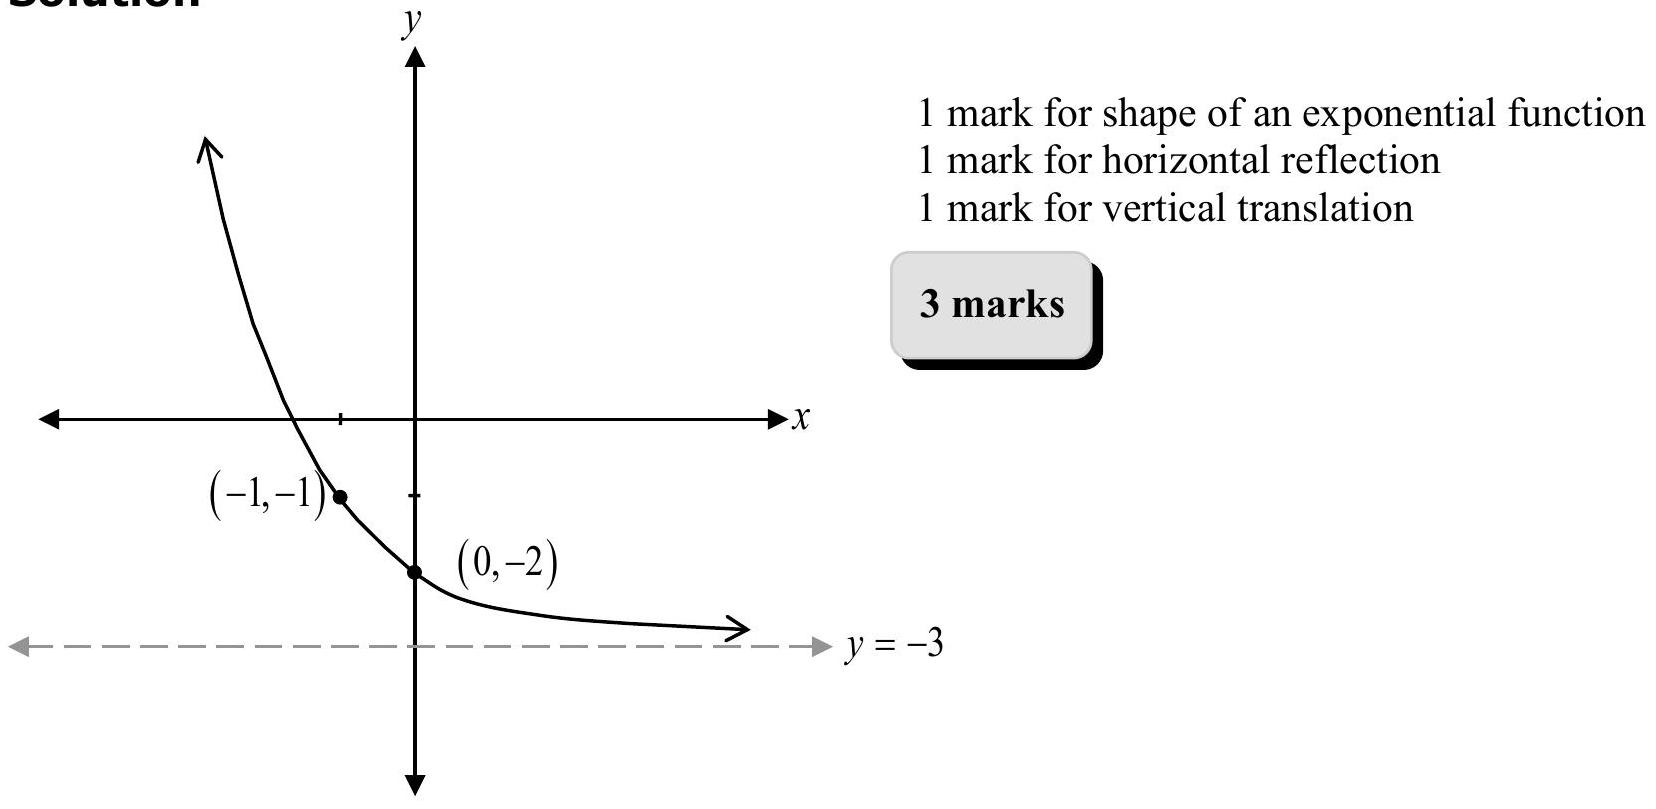
\includegraphics[max width=\textwidth, alt={}]{f67fedaf-ea11-42ad-a16e-f30d2fcf2bd3-362_809_1656_519_242}
\end{center}

Given the graph of $y=g(x)$, sketch the graph of $y=\frac{1}{g(x)}$.\\
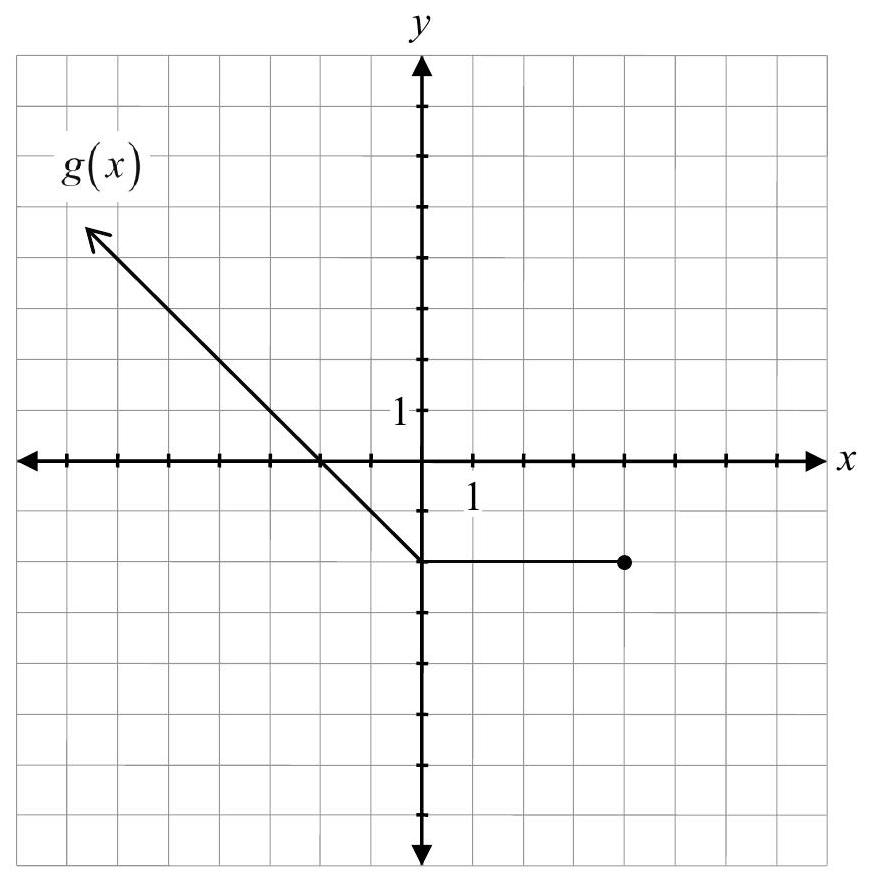
\includegraphics[max width=\textwidth, alt={}, center]{f67fedaf-ea11-42ad-a16e-f30d2fcf2bd3-363_880_875_489_247}

\section*{Solution}
\begin{center}
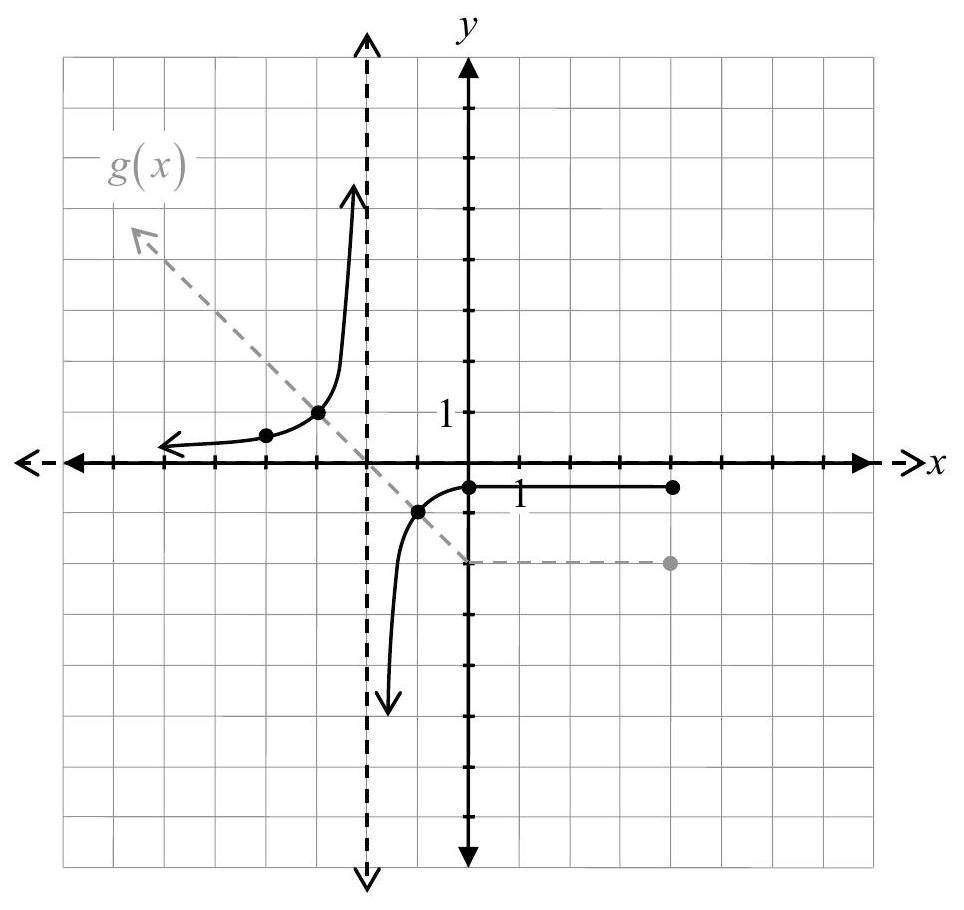
\includegraphics[max width=\textwidth, alt={}]{f67fedaf-ea11-42ad-a16e-f30d2fcf2bd3-363_910_964_1572_201}
\end{center}

1 mark for asymptotic behaviour approaching $x=-2\left(\frac{1}{2}\right.$ mark for each side $)$\\
$\frac{1}{2}$ mark for asymptotic behaviour approaching

$$
y=0
$$

$\frac{1}{2}$ mark for graph left of $x=-2$\\
$\frac{1}{2}$ mark for graph right of $x=-2$\\
$\frac{1}{2}$ mark for restricting domain\\
3 marks

Determine the exact value of $\tan \left(\frac{\pi}{12}\right)$.

\section*{Solution}
$$
\tan \left(\frac{\pi}{12}\right)=\tan \left(\frac{4 \pi}{12}-\frac{3 \pi}{12}\right)
$$

$\tan \left(\frac{\pi}{3}-\frac{\pi}{4}\right)=\frac{\tan \frac{\pi}{3}-\tan \frac{\pi}{4}}{1+\tan \frac{\pi}{3} \tan \frac{\pi}{4}} \quad 1$ mark for substitution into correct identity

$$
=\frac{\sqrt{3}-1}{1+\sqrt{3}} \quad 1 \text { mark for exact values }(1 / 2 \text { mark for each value })
$$

or

$$
=2-\sqrt{3}
$$

or

$$
=\frac{3-\sqrt{3}}{3+\sqrt{3}}
$$

Note:

\begin{itemize}
  \item Other combinations are possible.
\end{itemize}

Explain why the graph of $g(x)=\frac{3}{x^{2}+4}$ does not have a vertical asymptote.

\section*{Solution}
The graph of a rational function has a vertical asymptote when the denominator is equal to zero. The denominator of $g(x)$ will never be equal to zero.\\
□\\
1 mark

Solve, algebraically.

$$
\log _{3} x+\log _{3}(x+8)=2
$$

\section*{Solution}
\section*{Method 1}
$$
\begin{aligned}
\log _{3}[x(x+8)] & =2 \\
x^{2}+8 x & =3^{2} \\
x^{2}+8 x-9 & =0 \\
(x+9)(x-1) & =0 \\
x \geq-9 \quad x & =1
\end{aligned}
$$

1 mark for product law

1 mark for exponential form\\
$\frac{1}{2}$ mark for the permissible value of $x \frac{1}{2}$ mark for showing the rejection of the extraneous root

\section*{3 marks}
\section*{Method 2}
$$
\begin{aligned}
\log _{3} x+\log _{3}(x+8) & =\log _{3} 3^{2} \\
\log _{3}[x(x+8)] & =\log _{3} 9 \\
x^{2}+8 x & =9 \\
x^{2}+8 x-9 & =0 \\
(x+9)(x-1) & =0 \\
x \geq-9 \quad x & =1
\end{aligned}
$$

1 mark for logarithmic form\\
1 mark for product law\\
$\frac{1}{2}$ mark for the permissible value of $x$\\
$\frac{1}{2}$ mark for showing the rejection of the extraneous root

Sketch at least one period of the graph of the function $y=\sin \left(3\left(x+30^{\circ}\right)\right)-1$.

\section*{Solution}
\begin{center}
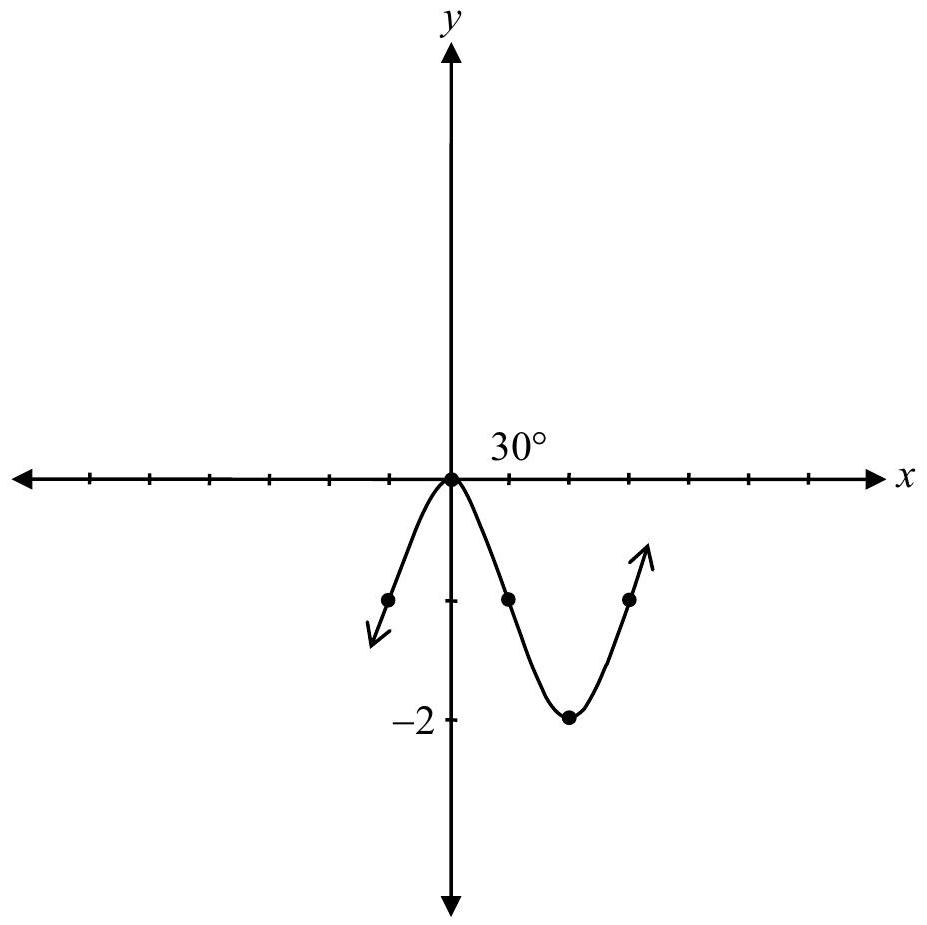
\includegraphics[max width=\textwidth, alt={}]{f67fedaf-ea11-42ad-a16e-f30d2fcf2bd3-367_925_927_584_313}
\end{center}

1 mark for shape of a sinusoidal function with correct amplitude\\
1 mark for period\\
1 mark for horizontal translation\\
1 mark for vertical translation\\
4 marks

Explain why the domain of the function, $f(x)=\log (x-3)$, is $x>3$.

\section*{Solution}
The argument of a logarithm cannot be negative or zero.

Sketch the graph of $p(x)=-(x-3)(x+1)^{2}(x-5)$.

\section*{Solution}
\begin{center}
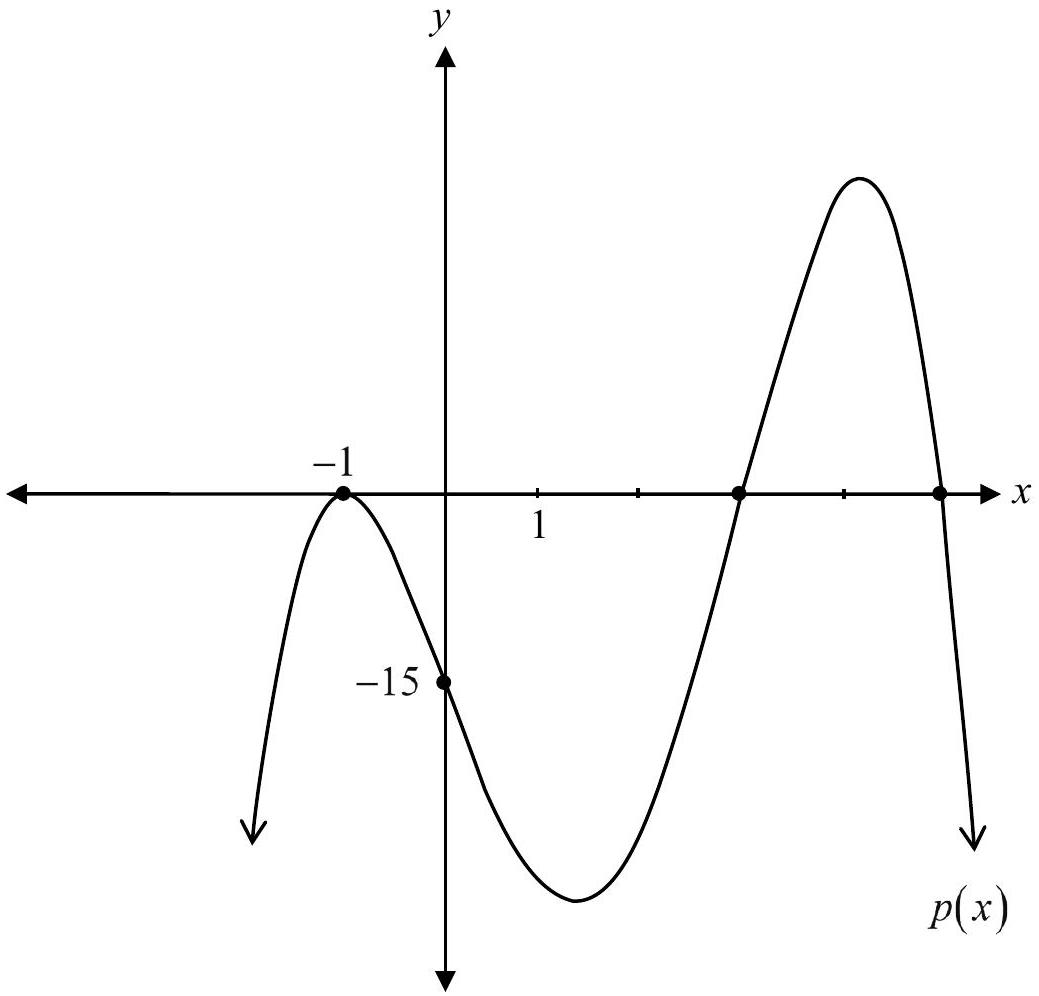
\includegraphics[max width=\textwidth, alt={}]{f67fedaf-ea11-42ad-a16e-f30d2fcf2bd3-369_996_1039_592_244}
\end{center}

1 mark for $x$-intercepts\\
1 mark for multiplicity of 2 at $x=-1$\\
$\frac{1}{2}$ mark for end behaviour\\
$\frac{1}{2}$ mark for $y$-intercept

Given that $\sin \theta=-\frac{2}{3}$ and $\tan \theta>0$, determine the exact value of $\sin 2 \theta$.

\section*{Solution}
$$
\begin{array}{rlr}
x^{2} & =r^{2}-y^{2} & \\
x^{2} & =9-4 & \\
x^{2} & =5 & \\
x & = \pm \sqrt{5} & \\
x & =-\sqrt{5} \text { mark for value of } x \\
\cos \theta & =-\frac{\sqrt{5}}{3} & \\
\sin 2 \theta & =2 \sin \theta \cos \theta & \\
& =2\left(-\frac{2}{3}\right)\left(-\frac{\sqrt{5}}{3}\right) & \\
& =\frac{4 \sqrt{5}}{9} & \mathbf{2} \text { mark for value of } \cos \theta \\
&
\end{array}
$$

Note:

\begin{itemize}
  \item Accept any of the following values for $x: x= \pm \sqrt{5}, x=-\sqrt{5}$, or $x=\sqrt{5}$.
\end{itemize}

Justify whether $\frac{5 \pi}{8}$ and $-\frac{11 \pi}{4}$ are coterminal angles.

\section*{Solution}
\section*{Method 1}
$\frac{5 \pi}{8}-\left(-\frac{11 \pi}{4}\right)$\\
$\frac{5 \pi}{8}+\frac{11 \pi}{4}$\\
$\frac{5 \pi}{8}+\frac{22 \pi}{8}$\\
$\frac{27 \pi}{8}$\\
Since $\frac{27 \pi}{8}$ is not a multiple of $2 \pi$ they are not coterminal angles.

\section*{Method 2}
Coterminal angles of $\frac{5 \pi}{8}$ :\\
$\frac{5 \pi}{8}-\frac{16 \pi}{8}=-\frac{11 \pi}{8}$\\
$-\frac{11 \pi}{8}-\frac{16 \pi}{8}=-\frac{27 \pi}{8}$\\
Coterminal angles of $-\frac{11 \pi}{4}$ :\\
$-\frac{11 \pi}{4}\left(\frac{2}{2}\right)=-\frac{22 \pi}{8}$\\
∴ Angles are not coterminal since $-\frac{27 \pi}{8} \neq-\frac{22 \pi}{8}$.

Sketch the graph of $f(x)=\frac{-2 x(x+1)(x-3)}{2 x}$.

\section*{Solution}
\begin{center}
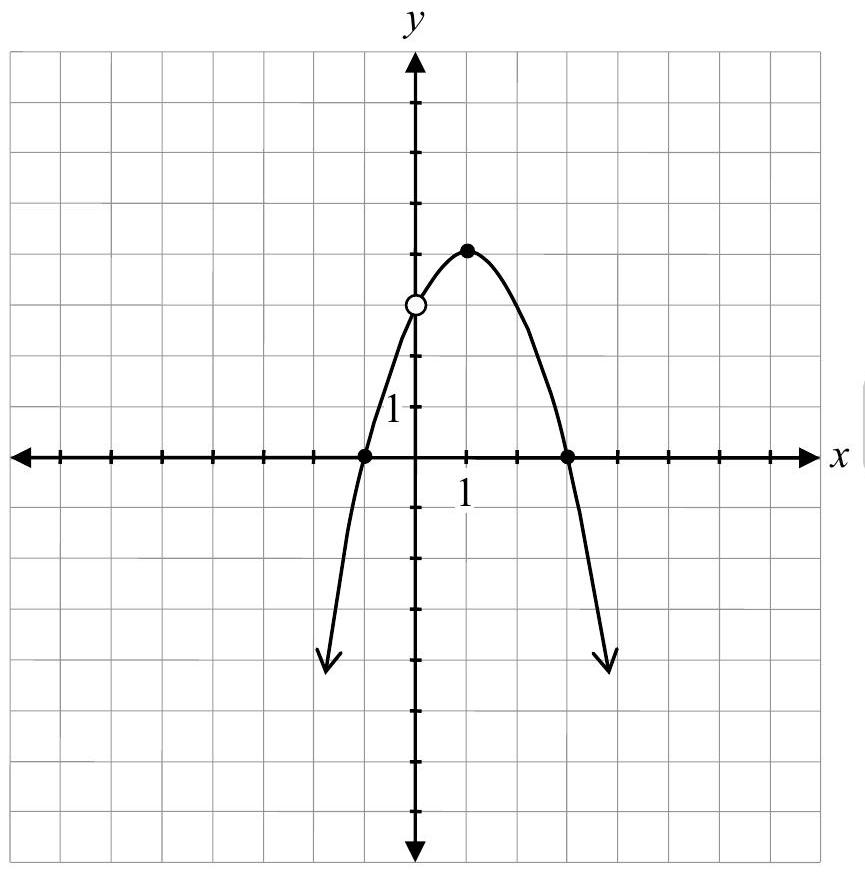
\includegraphics[max width=\textwidth, alt={}]{f67fedaf-ea11-42ad-a16e-f30d2fcf2bd3-372_876_865_605_240}
\end{center}

1 mark for point of discontinuity (hole) at $x=0 \frac{1}{2}$ mark for shape of a parabola with correct $x$-intercepts $\frac{1}{2}$ mark for end behaviour

Note:

\begin{itemize}
  \item Deduct $\frac{1}{2}$ mark for procedural error (incorrect $y$-value for point of discontinuity (hole)).
\end{itemize}

Given $\frac{\sin \theta+\cos \theta \csc \theta}{\sin \theta}$, determine the non-permissible values of $\theta$, where $\theta \in \mathbb{R}$.

\section*{Solution}
\section*{Method 1}
$\sin \theta=0 \quad \frac{1}{2}$ mark for $\sin \theta=0$\\
$\theta=0, \pi, 2 \pi \quad \frac{1}{2}$ mark for any non-permissible value of $\theta$\\
$\theta=\pi k, k \in \mathbb{Z} \quad 1$ mark for all non-permissible values of $\theta$\\

\includegraphics[max width=\textwidth, alt={}, center]{f67fedaf-ea11-42ad-a16e-f30d2fcf2bd3-373_134_229_917_620}

\section*{Method 2}
$\sin \theta=0 \quad \frac{1}{2}$ mark for $\sin \theta=0$\\
$\theta=0, \pi, 2 \pi \quad \frac{1}{2}$ mark for any non-permissible value of $\theta$\\
$\left.\begin{array}{l}\theta=2 \pi k, k \in \mathbb{Z} \\ \theta=\pi+2 \pi k, k \in \mathbb{Z}\end{array}\right\} \quad 1$ mark for all non-permissible values of $\theta$\\
2 marks

Write an equation of a rational function that has a horizontal asymptote at $y=0$ and a vertical asymptote at $x=6$.

\section*{Solution}
$$
f(x)=\frac{1}{x-6} \quad \begin{aligned}
& 1 \text { mark for horizontal asymptote } \\
& 1 \text { mark for vertical asymptote }
\end{aligned}
$$

Note:

\begin{itemize}
  \item Other answers are possible.
\end{itemize}

Given the functions $f(x)=\sqrt{x-1}$ and $g(x)=x^{2}$,\\
a) state the equation of $g(f(x))$.\\
b) sketch the graph of $g(f(x))$.

\section*{Solution}
a) $g(f(x))=x-1, x \geq 1$\\
b)\\
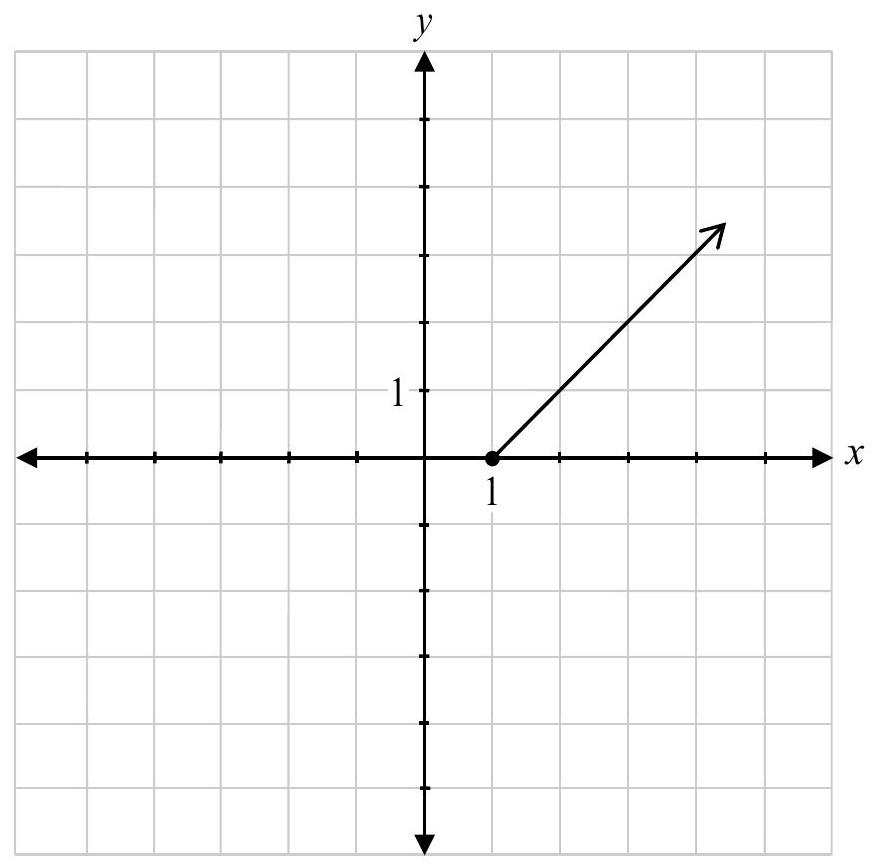
\includegraphics[max width=\textwidth, alt={}, center]{f67fedaf-ea11-42ad-a16e-f30d2fcf2bd3-375_865_875_1091_249}

1 mark for shape of graph consistent with a) 1 mark for restricted domain

\section*{Notes:}
\begin{itemize}
  \item Deduct a maximum of 1 mark for the concept error of not restricting the domain.
  \item Deduct $\frac{1}{2}$ mark for procedural error (not stating domain) if graph shows correct domain.
\end{itemize}

Suzanne was asked to determine the value of $\tan \theta$, given that $\sec \theta=-\frac{8}{3}$ and $\theta$ terminates in quadrant II.

Her solution:

$$
\begin{aligned}
(-3)^{2}+y^{2} & =(8)^{2} \\
y^{2} & =55 \\
y & =\sqrt{55} \\
\tan \theta & =\frac{\sqrt{55}}{3}
\end{aligned}
$$

Describe her error.

\section*{Solution}
Suzanne did not consider that the value of $\tan \theta$ is negative in quadrant II.\\
□\\
1 mark

Given the graph of $y=f(x)$, sketch the graph of $y=\sqrt{f(x)}$.

\section*{Solution}
\begin{center}
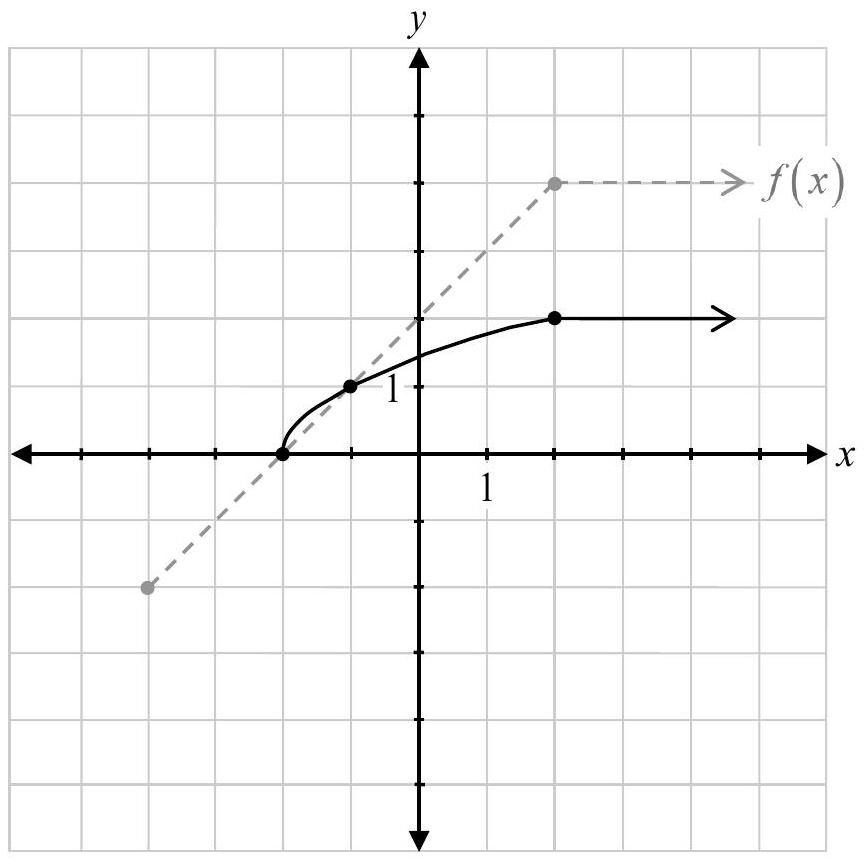
\includegraphics[max width=\textwidth, alt={}]{f67fedaf-ea11-42ad-a16e-f30d2fcf2bd3-377_862_867_541_257}
\end{center}

1 mark for restricting domain $\frac{1}{2}$ mark for shape between invariant points $\frac{1}{2}$ mark for shape to the right of invariant points\\
□ 2 marks

The point $P(\theta)=(0,-1)$ lies on the unit circle. State the angle $\theta$, over the interval $[2 \pi, 4 \pi]$.

\section*{Solution}
$\theta=\frac{7 \pi}{2}$\\
1 mark

Describe how the transformations of $f(x)$ on the graphs of $g(x)=f(3 x-6)$ and $h(x)=f(3(x-6))$ are different.

\section*{Solution}
The graph of $g(x)$ is a horizontal translation of $f(x)$ two units to the right and the graph of $h(x)$ is a horizontal translation of $f(x)$ six units to the right.\\
□\\
1 mark\\
a) Solve.

$$
\sqrt{2 x+5}-3=0
$$

b) Describe how the solution in a) relates to the graph of $y=\sqrt{2 x+5}-3$.

\section*{Solution}
a) $(\sqrt{2 x+5})^{2}=3^{2}$

$$
\begin{aligned}
2 x+5 & =9 \\
2 x & =4 \\
x & =2 \quad \text { 1 mark }
\end{aligned}
$$

b) The solution is the $x$-intercept of the graph.

Determine all of the zeros of the function $p(x)=x^{3}-2 x^{2}-9 x+18$.

\section*{Solution}
$$
\begin{aligned}
p(2) & =2^{3}-2(2)^{2}-9(2)+18 \quad 1 \text { mark for identifying one possible zero of } p(x) \\
& =0
\end{aligned}
$$

$\therefore(x-2)$ is a factor of $p(x)$

\begin{center}
\begin{tabular}{c|cccc}
2 & 1 & -2 & -9 & 18 \\
 &  & 2 & 0 & -18 \\
\hline
 & 1 & 0 & -9 & 0 \\
\hline
\end{tabular}
\end{center}

1 mark for synthetic division (or equivalent strategy)

$$
\begin{aligned}
& (x-2)\left(x^{2}-9\right)=0 \\
& (x-2)(x-3)(x+3)=0 \\
& x=2, x=3, x=-3
\end{aligned}
$$

$\frac{1}{2}$ mark for consistent factors\\
$\frac{1}{2}$ mark for consistent zeros

Given that the point $\left(\frac{\sqrt{23}}{6}, y\right)$ is on the unit circle, determine the exact value(s) of $y$.

\section*{Solution}
$\left(\frac{\sqrt{23}}{6}\right)^{2}+y^{2}=1 \quad 1 / 2$ mark for substitution\\
$\frac{23}{36}+y^{2}=1$\\
$y^{2}=\frac{36}{36}-\frac{23}{36}$\\
$y= \pm \frac{\sqrt{13}}{6}$\\
$\frac{1}{2}$ mark for exact values of $y$\\
1 mark

State one zero of the function $y=\tan x$.

\section*{Solution}
Any solution where $x=\pi k, k \in \mathbb{Z}$, is acceptable.

\section*{Question 1}
Youyi wants to buy a new cell phone from a company that offers 33 different types of cell phones. Each cell phone is available in 5 different colours. Determine the total number of available options.

\section*{Solution}
$\underline{33} \bullet \underline{5}=165$ options\\
1 mark

Determine the central angle subtended by an arc length of 30 cm on a circle with a diameter of 20.6 cm . Express your answer in degrees.

\section*{Solution}
$$
\begin{aligned}
s & =\theta r \\
30 & =\theta(10.3) \\
\theta & =2.912621 \ldots \\
\theta & =(2.912621)\left(\frac{180^{\circ}}{\pi}\right) \\
\theta & =166.880911 \ldots{ }^{\circ} \\
\theta & =166.881^{\circ}
\end{aligned}
$$

1 mark for substitution

1 mark for conversion

2 marks

A choir has 14 sopranos. Karin and Ellen are two of them. Determine the number of possible ensembles of 3 sopranos that could be formed if either Karin or Ellen, or both, must be included.

\section*{Solution}
\section*{Method 1}
Case 1: ${ }_{1} C_{1} \bullet{ }_{12} C_{2}=66$\\
1 mark for Case 1 and Case 2\\
Case 2 : ${ }_{1} C_{1} \cdot{ }_{12} C_{2}=66$\\
Case 3: ${ }_{2} C_{2} \cdot{ }_{12} C_{1}=12$\\
1 mark for Case 3\\
$66+66+12=144$\\
1 mark for addition of cases

\section*{3 marks}
\section*{Method 2}
${ }_{14} C_{3}-{ }_{12} C_{3}=144$\\
1 mark for ${ }_{14} C_{3}$\\
1 mark for ${ }_{12} C_{3}$\\
1 mark for subtraction of cases

3 marks

Loïc invests $\$ 5000$ at an annual interest rate of $6.75 \%$ compounded semi-annually. The value of his investment grows according to the following formula:

$$
A=P\left(1+\frac{r}{n}\right)^{n t}
$$

where $A$ is the value of the investment after $t$ years\\
$P$ is the amount of the initial deposit\\
$r$ is the annual interest rate (as a decimal)\\
$n$ is the number of compounding periods per year\\
$t$ is the time in years\\
Determine, algebraically, the length of time it will take Loïc's investment to grow to $\$ 9500$.

\section*{Solution}
$$
\begin{aligned}
9500 & =5000\left(1+\frac{0.0675}{2}\right)^{2 t} & & 1 / 2 \text { mark for substitution } \\
1.9 & =(1.03375)^{2 t} & & \\
\log 1.9 & =\log (1.03375) & & 1 \text { mark for applying logarithms } \\
\log 1.9 & =2 t \log 1.03375 & & 1 \text { mark for power law (or appropriate logarithm laws) } \\
t & =\frac{\log 1.9}{2 \log 1.03375} & & \\
t & =9.668522 \ldots & & 1 / 2 \text { mark for evaluating a quotient of logarithms } \\
t & =9.669 \text { years } & &
\end{aligned}
$$

\section*{Note:}
Accept $t=9.669$ years as a final answer (or consistent value of $t$ ).

Solve, algebraically, over the interval $[0,2 \pi]$.

$$
\csc ^{2} \theta-\csc \theta-6=0
$$

\section*{Solution}
\section*{Method 1}
$(\csc \theta-3)(\csc \theta+2)=0$\\
$\csc \theta=3 \quad \csc \theta=-2 \quad 1$ mark for solving for $\csc \theta$\\
$\sin \theta=\frac{1}{3} \quad \sin \theta=-\frac{1}{2} \quad 1$ mark for reciprocal\\
$\theta_{r}=0.339836 \ldots$\\
$\theta=0.340 ; 2.802 \quad \theta=\frac{7 \pi}{6}, \frac{11 \pi}{6}$\\
2 marks for solving for $\theta$ ( $\frac{1}{2}$ mark for each value)

\section*{4 marks}
\section*{Method 2}
$\frac{1}{\sin ^{2} \theta}-\frac{1}{\sin \theta}-6=0$\\
1 mark for reciprocal\\
$1-\sin \theta-6 \sin ^{2} \theta=0$\\
$6 \sin ^{2} \theta+\sin \theta-1=0$\\
$(3 \sin \theta-1)(2 \sin \theta+1)=0$\\
$\sin \theta=\frac{1}{3}$\\
$\sin \theta=\frac{-1}{2}$\\
1 mark for solving for $\sin \theta$\\
$\theta_{r}=0.339836 \ldots$\\
$\theta=0.340 ; 2.802$\\
$\theta=\frac{7 \pi}{6}, \frac{11 \pi}{6}$\\
2 marks for solving for $\theta$ ( $\frac{1}{2}$ mark for each value)

4 marks

Determine how many 4 -digit numbers can be made using the digits $0,1,2,3,4$, and 5 , if the third digit must be 3 , and repetition is not allowed.

\section*{Solution}
$$
\frac{4}{\text { not } 0 \text { or } 3} \cdot \frac{4}{3} \cdot \frac{1}{3} \cdot \frac{3}{3}=48
$$

$\frac{1}{2}$ mark for restriction of first digit\\
$\frac{1}{2}$ mark for restriction of third digit\\
1 mark for fundamental counting principle

2 marks

Describe the transformations required to obtain the graph of the function $y=-4 f\left(\frac{1}{3} x\right)$ from the graph of $y=f(x)$.

\section*{Solution}
\begin{itemize}
  \item Reflection over the $x$-axis
  \item Vertical stretch by a factor of 4
  \item Horizontal stretch by a factor of 3
\end{itemize}

1 mark for vertical reflection\\
1 mark for vertical stretch\\
1 mark for horizontal stretch

\section*{3 marks}
Given the graph of $y=f(x)$, sketch the graph of $y=\sqrt{f(x)}$.

\section*{Solution}
\begin{center}
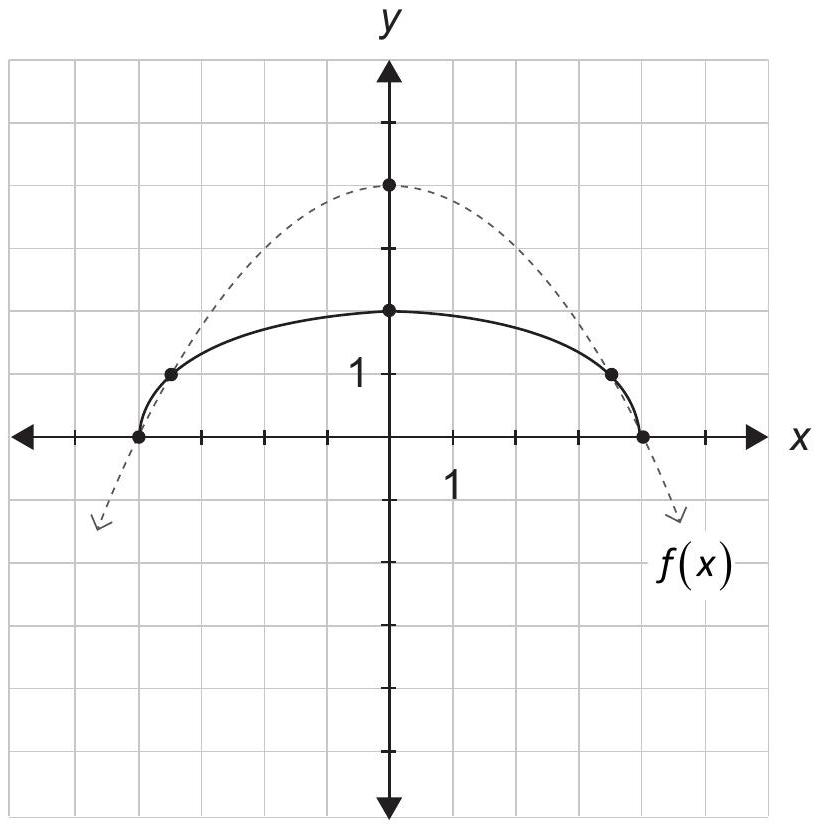
\includegraphics[max width=\textwidth, alt={}]{f67fedaf-ea11-42ad-a16e-f30d2fcf2bd3-391_828_820_584_242}
\end{center}

1 mark for restricting domain\\
$\frac{1}{2}$ mark for shape between invariant points, $\{0 \leq y \leq 1\}$\\
$\frac{1}{2}$ mark for shape above invariant points, $\{1 \leq y \leq 2\}$

2 marks

\section*{Question 9}
Describe how to determine if $(x-a)$ is a factor of the polynomial function, $p(x)$.

\section*{Solution}
$(x-a)$ is a factor of $p(x)$, if and only if $p(a)=0$.

1 mark

Express $\frac{1}{2} \log x-2 \log y+\log z$ as a single logarithm.

\section*{Solution}
$\log \left(\frac{\sqrt{x} \cdot z}{y^{2}}\right)$

1 mark for product law\\
1 mark for quotient law\\
1 mark for power law ( $\frac{1}{2}$ mark for each)

3 marks

Given the graph of $g(x)$, sketch the graph of $f(x)=\frac{1}{g(x)}$.\\
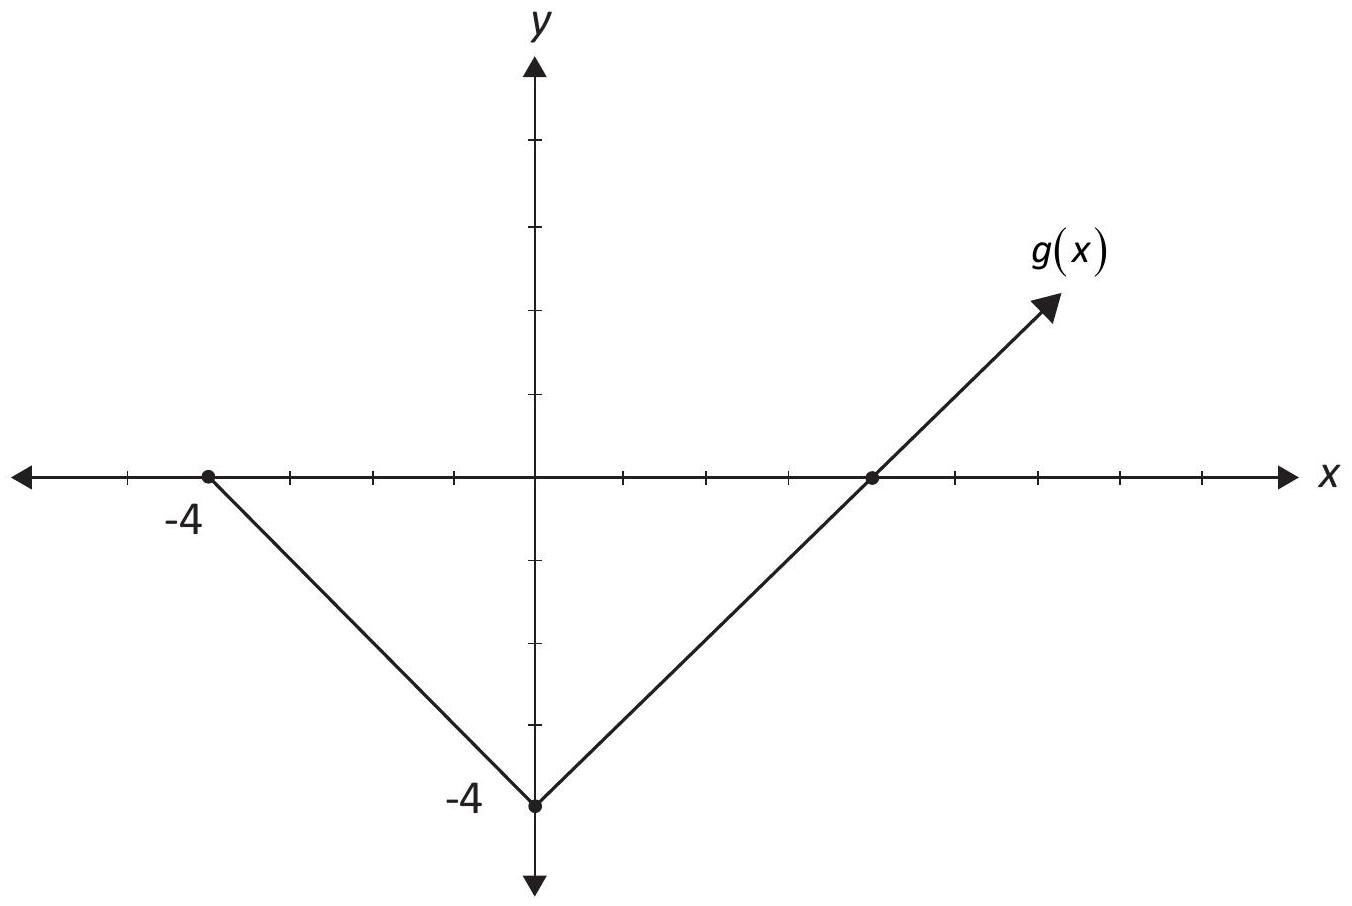
\includegraphics[max width=\textwidth, alt={}, center]{f67fedaf-ea11-42ad-a16e-f30d2fcf2bd3-394_906_1352_519_380}

\section*{Solution}
\begin{center}
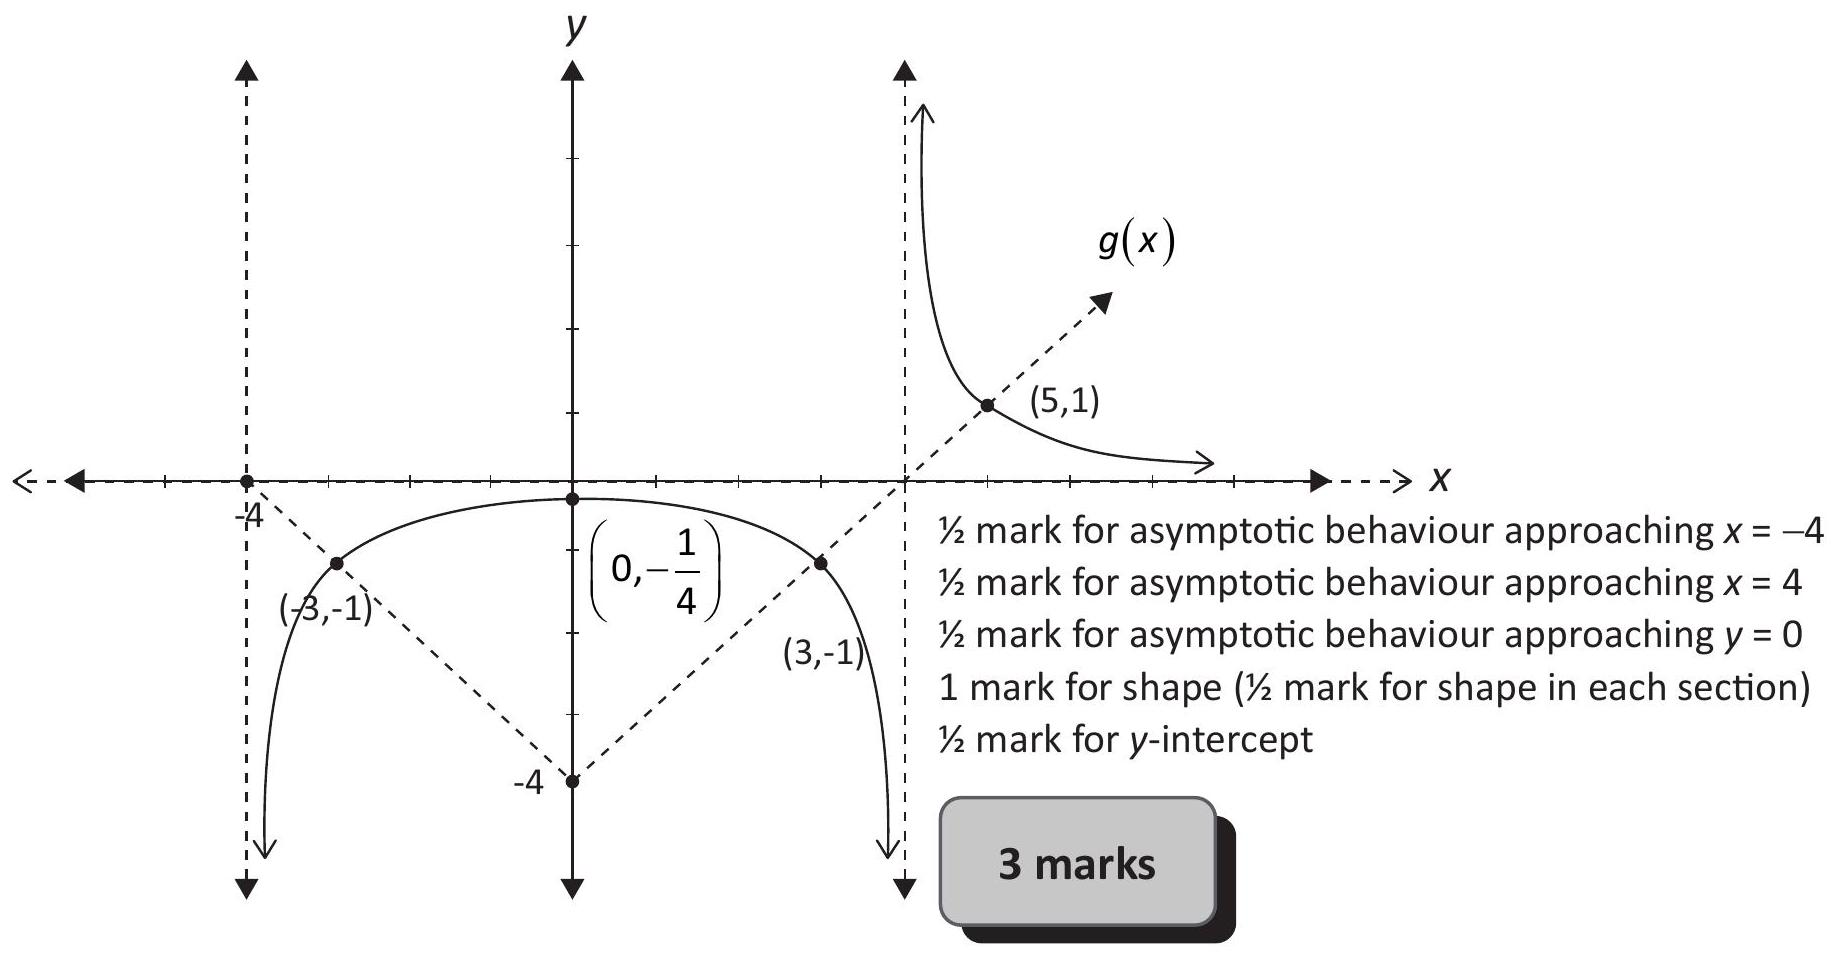
\includegraphics[max width=\textwidth, alt={}]{f67fedaf-ea11-42ad-a16e-f30d2fcf2bd3-394_955_1836_1533_165}
\end{center}

Given the identity $\frac{1-\tan ^{2} \theta}{\sec ^{2} \theta}=\cos 2 \theta$,\\
a) state a non-permissible value of $\theta$.\\
b) prove the identity for all permissible values of $\theta$.

\section*{Solution}
a) Any value where $\theta=\frac{\pi}{2}+k \pi, k \in \mathbb{Z}$ or $\theta=90^{\circ}+180^{\circ} k, k \in \mathbb{Z}$, is acceptable.\\
b)

\section*{Method 1}
\begin{center}
\begin{tabular}{|l|l|}
\hline
Left-Hand Side & Right-Hand Side \\
\hline
\( \frac{1-\frac{\sin ^{2} \theta}{\cos ^{2} \theta}}{\frac{1}{\cos ^{2} \theta}} 3 \frac{\cos ^{2} \theta-\sin ^{2} \theta}{\cos ^{2} \theta}{ }_{\frac{1}{\cos ^{2} \theta}}^{\frac{\cos ^{2} \theta}{\cos ^{2} \theta}} \frac{1}{\cos ^{2} \theta} \cos 2 \theta \) & $\cos 2 \theta$ \\
\hline
\end{tabular}
\end{center}

1 mark for correct substitution of identities\\
1 mark for algebraic strategies\\
1 mark for logical process to prove the identity

Determine an equation of the radical function represented by the graph of $f(x)$.\\
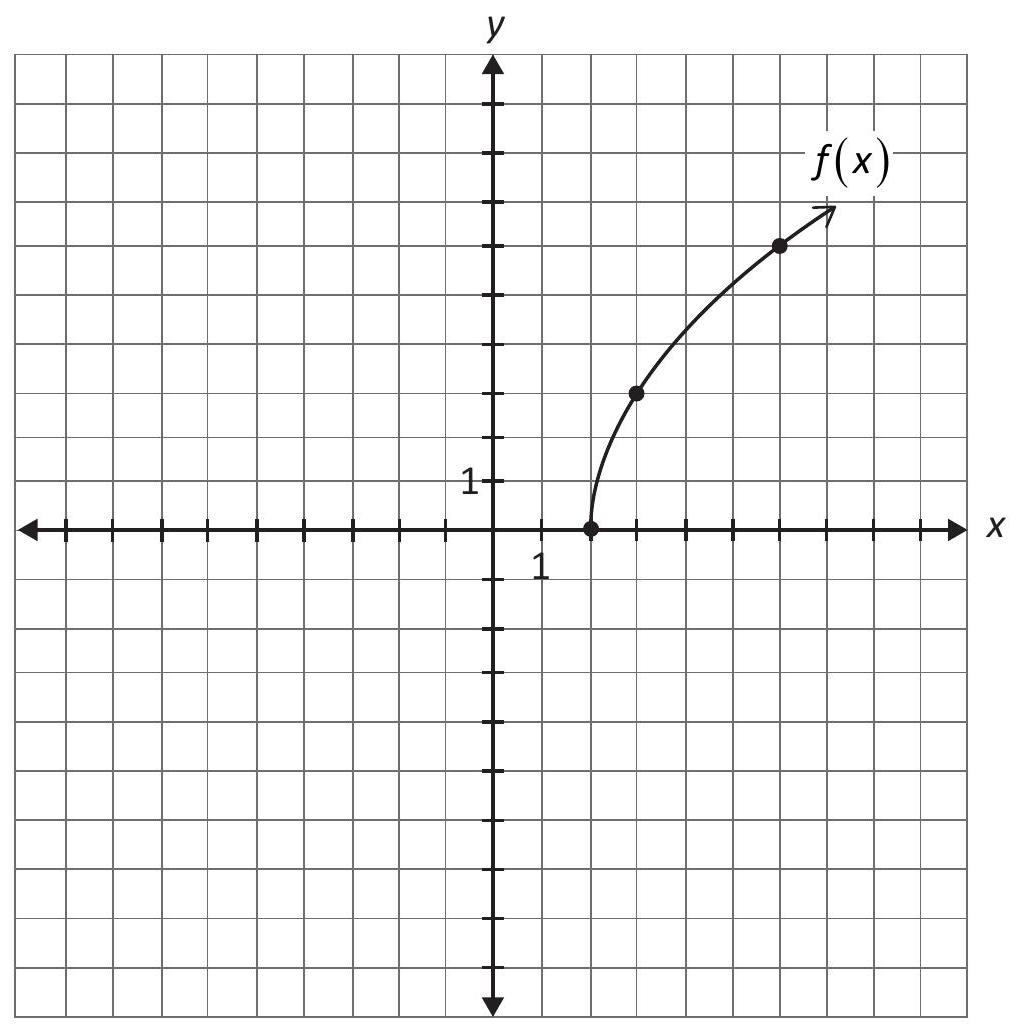
\includegraphics[max width=\textwidth, alt={}, center]{f67fedaf-ea11-42ad-a16e-f30d2fcf2bd3-396_1030_1017_472_558}

\section*{Solution}
$f(x)=3 \sqrt{x-2}$\\
1 mark for vertical stretch\\
1 mark for horizontal translation

2 marks

Given the graphs of $f(x)$ and $g(x)$, sketch the graph of $g(f(x))$.\\
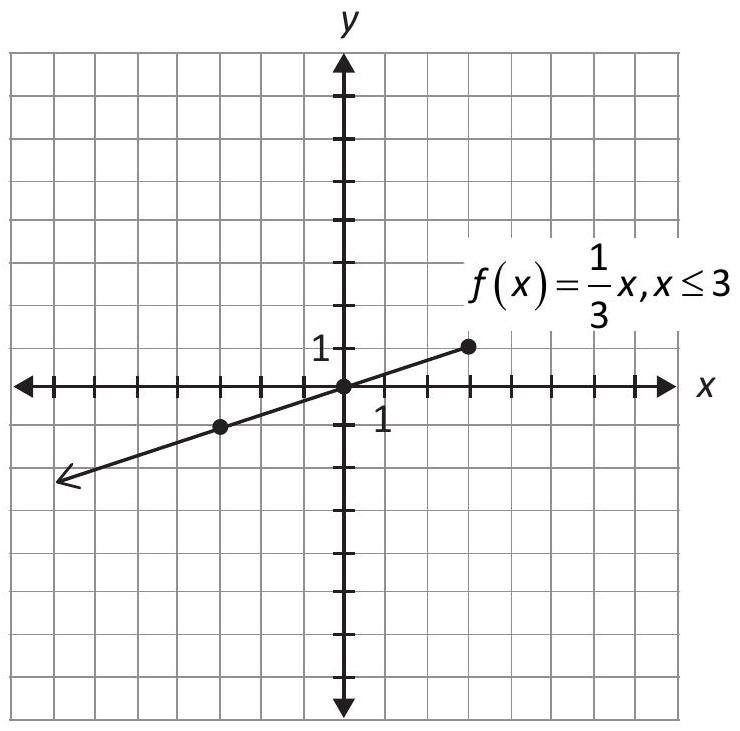
\includegraphics[max width=\textwidth, alt={}, center]{f67fedaf-ea11-42ad-a16e-f30d2fcf2bd3-397_731_740_481_294}\\
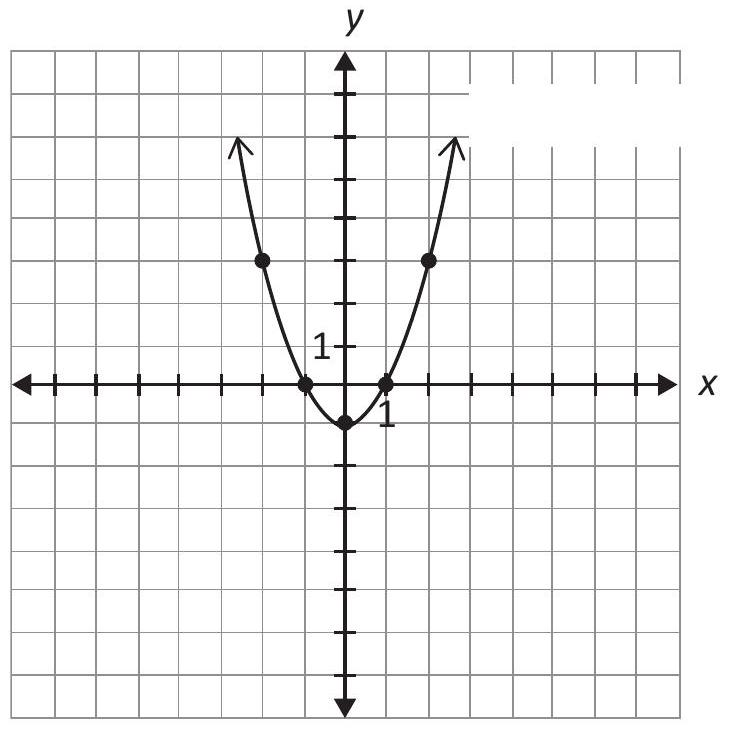
\includegraphics[max width=\textwidth, alt={}, center]{f67fedaf-ea11-42ad-a16e-f30d2fcf2bd3-397_729_729_483_1104}

\section*{Solution}
\begin{center}
\includegraphics[max width=\textwidth, alt={}]{f67fedaf-ea11-42ad-a16e-f30d2fcf2bd3-397_738_735_1344_696}
\end{center}

1 mark for $g(f(x))$\\
1 mark for restricted domain

\section*{2 marks}
Sketch a graph of $p(x)$ that satisfies all of the following conditions:

\begin{itemize}
  \item $p(x)$ is a polynomial function of degree 3
  \item $p(x)$ has a zero at -5 with a multiplicity of 2
  \item $p(x)$ has a zero at 1
  \item $p(x)$ has a leading coefficient of - 2
\end{itemize}

\section*{Solution}
\begin{center}
\includegraphics[max width=\textwidth, alt={}]{f67fedaf-ea11-42ad-a16e-f30d2fcf2bd3-398_982_1621_913_240}
\end{center}

Sketch the graph of $f(x)=\frac{x^{2}+x}{x}$.

\section*{Solution}
$f(x)=\frac{\not x(x+1)}{\not x}$\\
$f(x)=x+1, x \neq 0$\\
∴ there is a point of discontinuity(hole) at $(0,1)$.\\
\includegraphics[max width=\textwidth, alt={}, center]{f67fedaf-ea11-42ad-a16e-f30d2fcf2bd3-399_1048_1045_953_232}

1 mark for point of discontinuity (hole) at $x=0$\\
1 mark for shape of $y=x+1$

Identify the function that has a different range than $f(x)=x^{2}$.\\
a. $y=4 f(x)$\\
b. $y=f(x)+4$\\
c. $\quad y=f(x+4)$\\
d. $y=f(-x)$

Question 18\\
Identify the exact value of $\sin \left(-\frac{7 \pi}{3}\right)$.\\
a. $-\frac{\sqrt{3}}{2}$\\
b. $-\frac{1}{2}$\\
c. $\frac{1}{2}$\\
d. $\frac{\sqrt{3}}{2}$

\section*{Question 19}
Identify the value of $a$ in the equation, $\log _{a} 3=\frac{1}{4}$.\\
a. $\frac{1}{64}$\\
b. $3^{\frac{1}{4}}$\\
c. $\quad \mathbf{1 2}$\\
d. 81

Identify a value of $x$ where the graphs of $y=\cos x$ and $y=\sin x$ intersect.\\
a. $-\frac{3 \pi}{4}$\\
b. $-\frac{\pi}{4}$\\
c. 0\\
d. $\frac{3 \pi}{4}$

Question 21

Identify the number of negative terms in the binomial expansion of $(2 x-y)^{6}$.\\
a. 0\\
b. 3\\
c. 4\\
d. 6

Question 22

Identify the general solution of the equation, $\sin x=1$.\\
a. $x=k \pi, k \in \mathbb{Z}$\\
b. $x=2 k \pi, k \in \mathbb{Z}$\\
c. $\quad x=\frac{\pi}{2}+k \pi, k \in \mathbb{Z}$\\
d. $\quad x=\frac{\pi}{2}+2 k \pi, k \in \mathbb{Z}$

Identify a possible degree of the polynomial function represented below.\\
a. $\quad 2$\\
b. 3\\
c. 4\\
d. 5\\
\includegraphics[max width=\textwidth, alt={}, center]{f67fedaf-ea11-42ad-a16e-f30d2fcf2bd3-402_425_470_446_1011}

Question 24

Identify the expression that is equivalent to $\cos x \cot x$.\\
a. $\frac{1-\sin x}{\sin x}$\\
b. $\frac{\sin ^{2} x-1}{\sin x}$\\
C. $\sin x$\\
d. $\frac{1-\sin ^{2} x}{\sin x}$

\section*{Question 25}
Given that the point $(-7,-5)$ is on the graph of $y=g(x)$, identify the corresponding point on the graph of $y=|g(x)|$.\\
a. $(7,5)$\\
b. $(-7,5)$\\
c. $(7,-5)$\\
d. (-5, -7)

Given that $x=1$ is one of the zeros of $p(x)=x^{3}+x^{2}-10 x+8$, express $p(x)$ in completely factored form.

\section*{Solution}
$p(x)=x^{3}+x^{2}-10 x+8$

\begin{center}
\begin{tabular}{c|cccc}
1 & 1 & 1 & -10 & 8 \\
 & $\downarrow$ & 1 & 2 & -8 \\
\hline
 & 1 & 2 & -8 & 0 \\
\hline
\end{tabular}
\end{center}

1 mark for synthetic division (or any equivalent strategy)\\
$p(x)=(x-1)\left(x^{2}+2 x-8\right)$\\
$p(x)=(x-1)(x+4)(x-2)$\\
1 mark for consistent factors

2 marks

Determine the exact value of $\frac{\csc ^{2} \theta-1}{1-\cos ^{2} \theta}$ if $\theta=\frac{5 \pi}{6}$.

\section*{Solution}
\section*{Method 1}
$\frac{\csc ^{2}\left(\frac{5 \pi}{6}\right)-1}{1-\cos ^{2}\left(\frac{5 \pi}{6}\right)}$\\
$\frac{(2)^{2}-1}{1-\left(\frac{-\sqrt{3}}{2}\right)^{2}}$\\
1 mark for $\csc \left(\frac{5 \pi}{6}\right)$ ( $1 / 2$ mark for quadrant; $1 / 2$ mark for value)\\
1 mark for $\cos \left(\frac{5 \pi}{6}\right)(1 / 2$ mark for quadrant; $1 / 2$ mark for value)\\
$\frac{4-1}{1-\frac{3}{4}}$\\
$\frac{\frac{3}{1}}{\frac{1}{4}}$

\section*{2 marks}
12

\section*{Method 2}
$$
\begin{aligned}
& \frac{\cot ^{2} \theta}{\sin ^{2} \theta} \\
& \frac{\cot ^{2}\left(\frac{5 \pi}{6}\right)}{\sin ^{2}\left(\frac{5 \pi}{6}\right)} \\
& \frac{(-\sqrt{3})^{2}}{\left(\frac{1}{2}\right)^{2}}
\end{aligned}
$$

1 mark for $\cot \left(\frac{5 \pi}{6}\right)(1 / 2$ mark for quadrant; $1 / 2$ mark for value)\\
$\frac{\frac{3}{1}}{\frac{1}{4}}$\\
1 mark for $\sin \left(\frac{5 \pi}{6}\right)\left(\frac{1}{2}\right.$ mark for quadrant; $1 / 2$ mark for value)

Solve, graphically.

$$
-2 x+5=\sqrt{x-1}
$$

\section*{Solution}
\begin{center}
\includegraphics[max width=\textwidth, alt={}]{f67fedaf-ea11-42ad-a16e-f30d2fcf2bd3-405_852_1039_655_244}
\end{center}

$$
y=-2 x+5
$$

$\therefore x=2$

1 mark for shape of a radical function\\
1 mark for horizontal translation\\
1 mark for $x$-value consistent with intersection point of the two graphs

3 marks

If $\log _{a} 2=p$ and $\log _{a} 5=q$, express $\log _{a} 40$ in terms of $p$ and $q$.

\section*{Solution}
$$
\begin{aligned}
\log _{a} 40 & =\log _{a}\left(2^{3} \cdot 5\right) & & \\
& =3 \log _{a} 2+\log _{a} 5 & & 1 \text { mark for power law } \\
& =3 p+q & & 1 \text { mark for product law }
\end{aligned}
$$

\section*{2 marks}
Describe how to sketch the graph of $y=f^{-1}(x)$, given the graph of a linear function, $y=f(x)$.

\section*{Solution}
The graph of $y=f^{-1}(x)$ is obtained by reflecting the graph of $y=f(x)$ over the line $y=x$.\\
or\\
To sketch the inverse, $y=f^{-1}(x)$, transform all points on the graph of $y=f(x)$ from $(x, y)$ to $(y, x)$.

Given that $\sin \alpha=-\frac{4}{5}$ where $\alpha$ is in quadrant III, and $\cos \beta=\frac{12}{13}$ where $\beta$ is in quadrant IV, determine the exact value of $\cos (\alpha-\beta)$.

\section*{Solution}
\includegraphics[max width=\textwidth, alt={}, center]{f67fedaf-ea11-42ad-a16e-f30d2fcf2bd3-408_377_368_683_247}\\
\includegraphics[max width=\textwidth, alt={}, center]{f67fedaf-ea11-42ad-a16e-f30d2fcf2bd3-408_375_369_678_691}

$$
\begin{aligned}
x^{2}+4^{2} & =5^{2} \\
x^{2} & =9 \\
x & = \pm 3
\end{aligned}
$$

$$
\begin{aligned}
12^{2}+y^{2} & =13^{2} \\
y^{2} & =25 \\
y & = \pm 5
\end{aligned}
$$

$\frac{1}{2}$ mark for value of $x$\\
$\frac{1}{2}$ mark for value of $y$

$$
\begin{aligned}
\cos (\alpha-\beta) & =\cos \alpha \cos \beta+\sin \alpha \sin \beta \\
& =\left(-\frac{3}{5}\right)\left(\frac{12}{13}\right)+\left(-\frac{4}{5}\right)\left(-\frac{5}{13}\right) \\
& =\frac{-36+20}{65} \\
& =-\frac{16}{65}
\end{aligned}
$$

$\frac{1}{2}$ mark for consistent value of $\cos \alpha$\\
$\frac{1}{2}$ mark for consistent value of $\sin \beta$\\
1 mark for substitution into correct identity

\section*{Note:}
Accept any of the following values for $x: x= \pm 3 ; x=-3$; or $x=3$.\\
Accept any of the following values for $y: y= \pm 5 ; y=-5$; or $y=5$.

Sketch the graph of $f(x)=\frac{2 x-4}{x+1}$.

\section*{Solution}
\begin{center}
\includegraphics[max width=\textwidth, alt={}]{f67fedaf-ea11-42ad-a16e-f30d2fcf2bd3-409_972_983_603_242}
\end{center}

1 mark for asymptotic behaviour approaching $x=-1$\\
1 mark for asymptotic behaviour approaching $y=2$\\
1 mark for shape of rational function\\
( $\frac{1}{2}$ mark for graph left of $x=-1,1 / 2$ mark for graph right of $x=-1$ )

3 marks

Due to the tidal variations, the depth of the water in a bay is represented by the function,

$$
d(t)=-2 \cos \left[\frac{\pi}{6}(t+4)\right]+16
$$

where $d$ is the depth of the water, in metres and $t$ is the time, in hours.\\
a) Determine the depth of the water when $t=2$.\\
b) State the minimum depth of the water.\\
c) Determine the length of time between two consecutive low tides (minimum depths).

\section*{Solution}
a) $d(2)=-2 \cos \left[\frac{\pi}{6}(2+4)\right]+16$

$$
\begin{aligned}
& =-2 \cos \pi+16 \\
& =-2(-1)+16 \\
& =18 \text { metres }
\end{aligned}
$$

\section*{1 mark}
b) 14 metres

1 mark\\
c) period $=\frac{2 \pi}{\frac{\pi}{6}}$\\
$=12$ hours

1 mark for period\\
\includegraphics[max width=\textwidth, alt={}, center]{f67fedaf-ea11-42ad-a16e-f30d2fcf2bd3-410_184_310_2023_857}

Evaluate.

$$
\sin ^{2}\left(\frac{5 \pi}{4}\right) \sec \left(\frac{13 \pi}{3}\right)-\cot \left(\frac{7 \pi}{4}\right)
$$

\section*{Solution}
$$
\begin{array}{cl}
\left(-\frac{\sqrt{2}}{2}\right)^{2}\left(\frac{2}{1}\right)-(-1) & 1 \text { mark for } \sin \left(\frac{5 \pi}{4}\right)(1 / 2 \text { mark for value; } 1 / 2 \text { mark for quadrant }) \\
1+1 & 1 \text { mark for } \sec \left(\frac{13 \pi}{3}\right)(1 / 2 \text { mark for value; } 1 / 2 \text { mark for quadrant }) \\
2 & 1 \text { mark for } \cot \left(\frac{7 \pi}{4}\right)(1 / 2 \text { mark for value; } 1 / 2 \text { mark for quadrant })
\end{array}
$$

\section*{3 marks}
a) State the non-permissible value(s) of the function, $f(x)=\frac{x-3}{x^{2}-9}$.\\
b) Describe what each non-permissible value represents on the graph of $f(x)=\frac{x-3}{x^{2}-9}$.

\section*{Solution}
a) $x=3,-3$ 1 mark for non-permissible values ( $\frac{1}{2}$ mark for each)

\section*{1 mark}
b) At $x=3$, there is a point of discontinuity (hole) on the graph of $f(x)$. At $x=-3$, there is a vertical asymptote on the graph of $f(x)$.\\
$\frac{1}{2}$ mark for point of discontinuity (hole) at $x=3$\\
$\frac{1}{2}$ mark for vertical asymptote at $x=-3$

1 mark

Determine which of the given values is greater. Justify your answer.

$$
\log _{3} 38 \text { or } \log _{4} 50
$$

\section*{Solution}
$3^{3}=27$\\
$3^{4}=81 \quad \log _{3} 38>3$\\
$4^{2}=16$\\
$4^{3}=64 \quad \log _{4} 50<3$\\
$\therefore \log _{3} 38$ is greater\\
1 mark for justification

1 mark

Determine if the point $\left(\frac{3}{4}, \frac{\sqrt{5}}{4}\right)$ is on the unit circle. Justify your answer.

\section*{Solution}
$x^{2}+y^{2}=1$

$$
\begin{aligned}
\text { LHS } & =\left(\frac{3}{4}\right)^{2}+\left(\frac{\sqrt{5}}{4}\right)^{2} \\
& =\frac{9}{16}+\frac{5}{16} \\
& =\frac{14}{16}
\end{aligned}
$$

$\frac{14}{16} \neq 1$\\
∴ The point is not on the unit circle.\\
1 mark for justification

1 mark

Determine which term contains $x^{5}$ in the binomial expansion of $\left(2 x+\frac{3}{x}\right)^{11}$.

\section*{Solution}
\section*{Method 1}
$x^{11},\left(x^{10}\right)\left(\frac{1}{x}\right),\left(x^{9}\right)\left(\frac{1}{x^{2}}\right), \ldots$\\
1 mark for determining a pattern\\
$x^{11}, x^{9}, x^{7}, \ldots$\\
∴ The fourth term contains $x^{5}$.\\
1 mark for fourth term (or a term consistent with the pattern)

\section*{2 marks}
\section*{Method 2}
$$
\begin{aligned}
(x)^{11-k}\left(x^{-1}\right)^{k} & =x^{5} \\
x^{11-2 k} & =x^{5} \\
11-2 k & =5 \\
6 & =2 k \\
k & =3
\end{aligned}
$$

$\frac{1}{2}$ mark for substitution\\
$\frac{1}{2}$ mark for solving for $k$\\
∴ The fourth term contains $x^{5}$.

1 mark for fourth term\\
(or a term consistent with the value of $k$ )

\section*{2 marks}
Sketch the graph of $y=2\left(3^{x}\right)+1$.

\section*{Solution}
\begin{center}
\includegraphics[max width=\textwidth, alt={}]{f67fedaf-ea11-42ad-a16e-f30d2fcf2bd3-416_940_966_571_240}
\end{center}

1 mark for shape of an increasing exponential function\\
1 mark for vertical stretch\\
1 mark for vertical translation

3 marks

Solve, algebraically.

$$
\log (2 x+1)=\log (x-2)+1
$$

\section*{Solution}
\section*{Method 1}
$$
\begin{array}{rlrl}
\log (2 x+1)-\log (x-2)=1 & & \\
\log \left(\frac{2 x+1}{x-2}\right) & =1 & & 1 \text { mark for quotient law } \\
10^{1} & =\frac{2 x+1}{x-2} & & 1 \text { mark for exponential form } \\
10 x-20 & =2 x+1 & & \mathbf{2} \text { marks } \\
8 x & =21 & &
\end{array}
$$

\section*{Method 2}
$$
\begin{aligned}
\log (2 x+1) & =\log (x-2)+\log 10 \\
\log (2 x+1) & =\log (10(x-2)) \\
2 x+1 & =10(x-2) \\
2 x+1 & =10 x-20 \\
21 & =8 x \\
x & =\frac{21}{8}
\end{aligned}
$$

$\frac{1}{2}$ mark for logarithmic form\\
1 mark for product law\\
$\frac{1}{2}$ mark for equating arguments

2 marks

Given the functions, $f(x)=x+2$ and $g(x)=x-2$,\\
a) state the equation of $h(x)=f(x) \bullet g(x)$.\\
b) sketch the graph of $h(x)=f(x) \cdot g(x)$.

\section*{Solution}
a) $h(x)=(x+2)(x-2)$\\
or\\
$h(x)=x^{2}-4$\\
b)\\
\includegraphics[max width=\textwidth, alt={}, center]{f67fedaf-ea11-42ad-a16e-f30d2fcf2bd3-418_899_899_1222_242}

\section*{1 mark}
1 mark for graph consistent with a)

1 mark

Given $p(x)=-2 x^{3}+3 x+1$, determine the remainder when $p(x)$ is divided by $(x-2)$.

\section*{Solution}
\section*{Method 1}
$p(2)=-2(2)^{3}+3(2)+1$\\
1 mark for remainder theorem\\
$p(2)=-2(8)+6+1$\\
$p(2)=-9$

\section*{1 mark}
\section*{Method 2}
\begin{center}
\begin{tabular}{c|cccc}
2 & -2 & 0 & 3 & 1 \\
 & $\downarrow$ & -4 & -8 & -10 \\
\hline
 & -2 & -4 & -5 & -9 \\
\hline
\end{tabular}
\end{center}

1 mark for synthetic division (or any equivalent strategy)

1 mark\\
∴ The remainder is.-9

Determine the equation of the sinusoidal function in the form $y=A \cos (B x)+D$.\\
\includegraphics[max width=\textwidth, alt={}, center]{f67fedaf-ea11-42ad-a16e-f30d2fcf2bd3-420_972_1206_517_457}

Solution\\
$y=6 \cos \left(\frac{\pi}{15} x\right)+4$\\
1 mark for the value of $A$\\
1 mark for the value of $B$ ( $\frac{1}{2}$ mark for period; $\frac{1}{2}$ mark for consistent value of $B$ )\\
1 mark for the value of $D$

3 marks

Determine the total number of arrangements of the letters in the word TORONTO.\\
State your answer as a whole number.

\section*{Solution}
\begin{center}
\begin{tabular}{cl}
$\frac{7!}{2!3!}$ & $\frac{1 / 2 \text { mark for } 7!}{1 / 2 \text { mark for division by } 2!3!}$ \\
$\frac{7 \cdot 6 \cdot 5 \cdot 4 \cdot 3!}{2!3!}$ & $\frac{1 / 2 \text { mark for factorial expansion }}{\frac{7 \cdot 6 \cdot 5 \cdot 4}{2}}$ \\
$7 \cdot 6 \cdot 5 \cdot 2$ &  \\
\end{tabular}
\end{center}

420\\
$\frac{1}{2}$ mark for consistent number of arrangements

Liam went for a ride on a Ferris wheel with a radius of 5 metres. Determine the distance he travelled if the Ferris wheel stopped after rotating $1260^{\circ}$.

\section*{Solution}
$\theta=1260^{\circ} \cdot \frac{\pi}{180^{\circ}}$\\
1 mark for conversion\\
$\theta=7 \pi$\\
or\\
$\theta=21.991148 \ldots$\\
$s=\theta r$\\
$s=7 \pi(5)$\\
1 mark for substitution\\
$s=35 \pi$ metres\\
or\\
$s=109.956$ metres\\
2 marks

Determine and simplify the term that contains $x^{12}$ in the binomial expansion of $\left(2 x^{4}-3\right)^{7}$.

\section*{Solution}
\section*{Method 1}
$$
\begin{aligned}
& \left(x^{4}\right)^{7},\left(x^{4}\right)^{6},\left(x^{4}\right)^{5}, \ldots \\
& 1 \text { mark for determining a pattern } \\
& x^{28}, x^{24}, x^{20}, \ldots \\
& t_{5}={ }_{7} C_{4}\left(2 x^{4}\right)^{3}(-3)^{4} \\
& 2 \text { marks ( } 1 \text { mark for }{ }_{7} C_{4} ; 1 / 2 \text { mark for each consistent factor) } \\
& =22680 x^{12} \\
& 1 \text { mark for simplification ( } \frac{1}{2} \text { mark for coefficient, } \frac{1}{2} \text { mark } \\
& \text { for exponent) }
\end{aligned}
$$

\section*{4 marks}
\section*{Method 2}
$$
\begin{aligned}
x^{12} & =\left(x^{4}\right)^{7-k}\left(x^{0}\right)^{k} & & 1 / 2 \text { mark for substitution } \\
12 & =28-4 k & & \\
-16 & =-4 k & & 1 / 2 \text { mark for solving for } k \\
4 & =k & & 2 \text { marks }\left(1 \text { mark for }{ }_{7} C_{4} ; 1 / 2 \text { mark for each consistent factor }\right) \\
t_{5} & ={ }_{7} C_{4}\left(2 x^{4}\right)^{3}(-3)^{4} & & 1 \text { mark for simplification }(1 / 2 \text { mark for coefficient, } 1 / 2 \text { mark } \\
& =22680 x^{12} & & \text { for exponent })
\end{aligned}
$$

4 marks

The normal healing of wounds can be modeled by an exponential function. The area of the wound decreases according to the formula,

$$
A=A_{0} e^{-0.35 t}
$$

where: $\quad A$ is the area of the wound in $\mathrm{cm}^{2}$, after $t$ days, $A_{0}$ is the initial area of the wound in $\mathrm{cm}^{2}$, and $t$ is the time, in days, after healing begins.

If a wound has an initial area of $25 \mathrm{~cm}^{2}$, determine:\\
a) the area of the wound after 3 days.\\
b) the amount of time it will take for the area of the wound to decrease to $4 \mathrm{~cm}^{2}$.

\section*{Solution}
a) $A=25 e^{-0.35(3)}$

$$
A=8.748 \mathrm{~cm}^{2}
$$

\section*{1 mark}
b) $4=25 e^{-0.35 t}$

$$
\begin{aligned}
0.16 & =e^{-0.35 t} & & \\
\ln 0.16 & =\ln e^{-0.35 t} & & 1 \text { mark for applying logarithms } \\
\ln 0.16 & =-0.35 t \ln e & & 1 / 2 \text { mark for power law } \\
\frac{\ln 0.16}{-0.35} & =t & & \\
t & =5.235947 \ldots & & 1 / 2 \text { mark for the value of } t \\
t & =5.236 \text { days } & &
\end{aligned}
$$

During a hockey practice, 4 players are wearing a green jersey and 5 players are wearing a red jersey. Determine the number of ways three players can be selected if at least two of the players must be wearing a red jersey.

\section*{Solution}
Case 1: ${ }_{5} C_{2} \cdot{ }_{4} C_{1}=40$\\
1 mark for Case 1

Case 2: ${ }_{5} C_{3} \cdot{ }_{4} C_{0}=10$\\
1 mark for Case 2\\
$40+10=50$ ways\\
1 mark for addition of cases

3 marks

\section*{Note:}
${ }_{4} C_{0}$ does not need to be shown.

Solve, algebraically, over the interval $[0,2 \pi]$.

$$
2 \sin ^{2} x+5 \cos x+1=0
$$

\section*{Solution}
$$
\begin{aligned}
2\left(1-\cos ^{2} x\right)+5 \cos x+1 & =0 & & 1 \text { mark for substitution of an appropriate identity } \\
2-2 \cos ^{2} x+5 \cos x+1 & =0 & & \\
-2 \cos ^{2} x+5 \cos x+3 & =0 & & \\
2 \cos ^{2} x-5 \cos x-3 & =0 & & \\
(2 \cos x+1)(\cos x-3) & =0 & & \\
\cos x=-\frac{1}{2} \quad \cos x & =3 & & 1 \text { mark for solving for } \cos x \\
x=\frac{2 \pi}{3}, \frac{4 \pi}{3} & \text { no solution } & \begin{array}{l}
2 \text { marks for solving for } x(1 / 2 \text { mark for each value; } 1 \text { mark } \\
\text { for indicating no solution })
\end{array} &
\end{aligned}
$$

\section*{4 marks}
The function, $y=f(x)$, has a domain of $[-8,4]$. The domain of the graph of $y=f(b x)$ is $[-4,2]$.\\
State the value of $b$.

\section*{Solution}
$b=2$

\section*{Question 7}
Describe the difference between the graph of $f(x)=\frac{(x+3)(x-4)}{(x+3)}$ and the graph of $g(x)=x-4$.

\section*{Solution}
The graph of $f(x)$ has a point of discontinuity at $x=-3$, where as the graph of $g(x)$ does not.

1 mark

Determine if the point $\left(-\frac{3}{5}, \frac{2}{\sqrt{3}}\right)$ is on the unit circle. Justify your answer.

\section*{Solution}
\section*{Method 1}
$x^{2}+y^{2}=1$

$$
\begin{aligned}
\text { Left-Hand Side } & =\left(-\frac{3}{5}\right)^{2}+\left(\frac{2}{\sqrt{3}}\right)^{2} \\
& =\frac{9}{25}+\frac{4}{3} \\
& =\frac{27}{75}+\frac{100}{75}
\end{aligned}
$$

$\frac{127}{75} \neq 1$\\
Therefore the point $\left(-\frac{3}{5}, \frac{2}{\sqrt{3}}\right)$ is not on the unit circle.\\
1 mark for justification

\section*{1 mark}
\section*{Method 2}
Since $\frac{2}{\sqrt{3}}>1$, the point is not on the unit circle.\\
1 mark for justification

1 mark

Given the graph of $f(x)$, sketch the graph of $g(x)=f(-(x-1))+3$.

\section*{Solution}
\begin{center}
\includegraphics[max width=\textwidth, alt={}]{f67fedaf-ea11-42ad-a16e-f30d2fcf2bd3-430_819_818_584_240}
\end{center}

1 mark for horizontal reflection\\
1 mark for horizontal translation\\
1 mark for vertical translation

Bonnie was asked to determine the factors of $p(x)=-3 x^{4}+2 x^{2}-4 x+5$.\\
Describe the error she made in her set up of synthetic division.\\
$1\left\lfloor\begin{array}{llll}-3 & 2 & -4 & 5\end{array}\right.$

\section*{Solution}
Bonnie did not write the coefficient of 0 for the missing term, $x^{3}$.

1 mark

Given the functions, $f(x)=\frac{1}{x-1}$ and $g(x)=x-3$,\\
a) state the equation of $f(g(x))$.\\
b) state the domain of $f(g(x))$.

\section*{Solution}
a) $f(g(x))=\frac{\frac{1}{x-4}}{}$\\
b) Domain: $\{x \mid x \neq 4, x \in \mathbb{R}\}$\\
or

Domain: $\underline{(-\infty, 4) \cup(4, \infty)}$

Prove the identity for all permissible values of $x$.

$$
\tan 2 x=\frac{2}{\cot x-\tan x}
$$

\section*{Solution}
\section*{Method 1}
\begin{center}
\begin{tabular}{|l|l|}
\hline
Left-Hand Side & Right-Hand Side \\
\hline
$\tan 2 x$ &  \\
\hline
 & $\frac{2}{\frac{\cos x}{\sin x}-\frac{\sin x}{\cos x}}$ \\
\hline
 & $\frac{2}{\frac{\cos ^{2} x-\sin ^{2} x}{\sin x \cos x}}$ \\
\hline
 & $\frac{2 \sin x \cos x}{\cos ^{2} x-\sin ^{2} x}$ \\
\hline
 & $\frac{\sin 2 x}{\cos 2 x}$ \\
\hline
 & $\tan 2 x$ \\
\hline
\end{tabular}
\end{center}

1 mark for correct substitution of appropriate identities\\
1 mark for algebraic strategies\\
1 mark for logical process to prove the identity

\section*{Method 2}
\begin{center}
\begin{tabular}{|l|l|}
\hline
Left-Hand Side & Right-Hand Side \\
\hline
$2 \tan x$ $\_\_\_\_$ &  \\
\hline
$1-\tan ^{2} x$ & \includegraphics[max width=\textwidth, alt={}]{f67fedaf-ea11-42ad-a16e-f30d2fcf2bd3-434_154_265_594_776}
 \\
\hline
 &  \\
\hline
\( \frac{\frac{2 \sin x}{\cos x}}{1-\frac{\sin ^{2} x}{\cos ^{2} x}} \) & \( \frac{2}{\frac{\cos ^{2} x-\sin ^{2} x}{\sin x \cos x}} \) \\
\hline
\( \frac{\frac{2 \sin x}{\cos x}}{\frac{\cos ^{2} x-\sin ^{2} x}{\cos ^{2} x}} \) & $\frac{2 \sin x \cos x}{\cos ^{2} x-\sin ^{2} x}$ \\
\hline
$\frac{2 \sin x \cos x}{\cos ^{2} x-\sin ^{2} x}$ &  \\
\hline
\end{tabular}
\end{center}

1 mark for correct substitution of appropriate identities\\
1 mark for algebraic strategies\\
1 mark for logical process to prove the identity

\section*{Method 3}
\begin{center}
\begin{tabular}{|l|l|}
\hline
Left-Hand Side & Right-Hand Side \\
\hline
$\frac{2 \tan x}{1-\tan ^{2} x}$ & $\frac{2}{\frac{1}{\tan x}-\tan x}$ \\
\hline
 & $\frac{2}{\frac{1-\tan ^{2} x}{\tan x}}$ \\
\hline
 & $\frac{2 \tan x}{1-\tan ^{2} x}$ \\
\hline
\end{tabular}
\end{center}

1 mark for correct substitution of appropriate identities\\
1 mark for algebraic strategies\\
1 mark for logical process to prove the identity

\section*{3 marks}
Given $f(x)=-x^{2}+2$ and $g(x)=x^{2}-1$,\\
a) determine the equation $h(x)=g(x)-f(x)$.\\
b) state the range of $h(x)$.

\section*{Solution}
a) $h(x)=g(x)-f(x)$

$$
\begin{aligned}
& h(x)=\left(x^{2}-1\right)-\left(-x^{2}+2\right) \\
& h(x)=x^{2}-1+x^{2}-2 \\
& h(x)=2 x^{2}-3
\end{aligned}
$$

b) Range: $\{y \mid y \geq-3, y \in \mathbb{R}\}$\\
or

1 mark for subtraction of $g(x)-f(x)$

1 mark

1 mark for range consistent with $h(x)$

Range: $[-3, \infty)$\\
1 mark

Given the graph of $f(x)$,\\
\includegraphics[max width=\textwidth, alt={}, center]{f67fedaf-ea11-42ad-a16e-f30d2fcf2bd3-437_641_637_457_743}\\
a) sketch the graph after a reflection over the line $y=x$.\\
b) state a restriction on the domain of $f(x)$ in order for its inverse to be a function.

\section*{Solution}
a)\\
\includegraphics[max width=\textwidth, alt={}, center]{f67fedaf-ea11-42ad-a16e-f30d2fcf2bd3-437_643_637_1383_287}\\
b) $\{x \mid x \geq-2, x \in \mathbb{R}\}$\\
or\\
$\{x \mid x \leq-2, x \in \mathbb{R}\}$

\section*{Note:}
Other answers are possible for b).

Describe a transformation of a function that would not affect its domain.

\section*{Solution}
vertical stretch by a factor of $a$\\
or\\
vertical reflection\\
or\\
vertical translation $k$ units up/down

Given the graph of $f(x)$, sketch the graph of the function $y=|f(x)|$.

\section*{Solution}
\begin{center}
\includegraphics[max width=\textwidth, alt={}]{f67fedaf-ea11-42ad-a16e-f30d2fcf2bd3-439_865_861_586_242}
\end{center}

Determine, algebraically, all of the zeros of the polynomial function, $p(x)=3 x^{3}+x^{2}-20 x+12$.

\section*{Solution}
$p(x)=3 x^{3}+x^{2}-20 x+12$\\
$p(2)=3(2)^{3}+(2)^{2}-20(2)+12$\\
$p(2)=0 \quad 1$ mark for identifying one zero of $p(x)$\\
$\therefore(x-2)$ is a factor

\begin{center}
\begin{tabular}{r|rrrr}
2 & 3 & 1 & -20 & 12 \\
 &  & 6 & 14 & -12 \\
\hline
 & 3 & 7 & -6 & 0 \\
\hline
\end{tabular}
\end{center}

1 mark for synthetic division (or equivalent strategy)

$$
\begin{array}{rlr}
p(x) & =(x-2)\left(3 x^{2}+7 x-6\right) & \\
0 & =(x-2)(3 x-2)(x+3) & 1 / 2 \text { mark for consistent factors } \\
x & =2, x=\frac{2}{3}, x=-3 & 1 / 2 \text { mark for consistent zeros }
\end{array}
$$

\section*{3 marks}
Given $\theta=240^{\circ}$, identify the coordinates of the point, $P(\theta)$, on the unit circle.\\
a. $\left(-\frac{\sqrt{3}}{2},-\frac{1}{2}\right)$\\
b. $\left(-\frac{\sqrt{2}}{2},-\frac{\sqrt{2}}{2}\right)$\\
c. $\left(-\frac{1}{2},-\frac{\sqrt{3}}{2}\right)$\\
d. $\left(\frac{1}{2},-\frac{\sqrt{3}}{2}\right)$

\section*{Question 19}
Given the functions, $f(x)=-3 x+5$ and $g(x)=x^{2}+x-1$, identify the value of $g(f(2))$.\\
a. -10\\
b. -5\\
c. -3\\
d. -1

Given $f(x)=\sqrt{x}+5$, identify the equation of the transformed graph that has the same $y$-intercept.\\
a. $\quad y=f(x-3)$\\
b. $\quad y=-3 f(x)$\\
c. $y=f(-3 x)$\\
d. $y=f(x)-3$

\section*{Question 21}
Given the graph of $p(x)=a x^{3}+b x^{2}+c x+d$, identify the statement that is true.\\
a. $\quad a>0, d<0$\\
b. $\quad a>0, d>0$\\
c. $\quad a<0, d<0$\\
d. $\quad a<0, d>0$\\
\includegraphics[max width=\textwidth, alt={}, center]{f67fedaf-ea11-42ad-a16e-f30d2fcf2bd3-442_429_476_1237_936}

\section*{Question 22}
Identify the general solution of the equation, $\csc \theta=-1$.\\
a. $\quad \theta=\frac{\pi}{2}+k \pi, k \in \mathbb{Z}$\\
b. $\quad \theta=\frac{3 \pi}{2}+2 k \pi, k \in \mathbb{Z}$\\
c. $\quad \theta=\frac{3 \pi}{2}+k \pi, k \in \mathbb{Z}$\\
d. $\theta=\pi+2 k \pi, k \in \mathbb{Z}$

Identify the equation of a radical function with a domain of $[-6, \infty)$ and a range of $(-\infty, 3]$.\\
a. $y=-\sqrt{x+6}-3$\\
b. $y=-\sqrt{x+6}+3$\\
c. $\quad y=\sqrt{-(x+3)}-6$\\
d. $y=\sqrt{x-6}+3$

\section*{Question 24}
Identify the value of $n$ in the equation, ${ }_{n} C_{3}={ }_{n} C_{7}$.\\
a. 3\\
b. 4\\
c. 7\\
d. 10

\section*{Question 25}
Identify the remainder when $p(x)=x^{5}-1$ is divided by $(x+1)$.\\
a. -2\\
b. -1\\
c. 0\\
d. 4

Match each function with its corresponding graph.

\section*{Solution}
Write the corresponding letter in this column.\\
$y=\sqrt{x}-3$\\
$y=\sqrt{-x}+3$\\
$y=-\sqrt{x+3}$\\
$y=-\sqrt{-(x-3)}$\\
$\_\_\_\_$\\
B\\
D

C\\
$\_\_\_\_$\\
A\\
$\frac{1}{2}$ mark for each correct answer

\section*{2 marks}
A)\\
\includegraphics[max width=\textwidth, alt={}, center]{f67fedaf-ea11-42ad-a16e-f30d2fcf2bd3-444_635_633_1125_367}\\
B)\\
\includegraphics[max width=\textwidth, alt={}, center]{f67fedaf-ea11-42ad-a16e-f30d2fcf2bd3-444_633_633_1125_1250}\\
C)\\
\includegraphics[max width=\textwidth, alt={}, center]{f67fedaf-ea11-42ad-a16e-f30d2fcf2bd3-444_633_631_1800_369}\\
D)\\
\includegraphics[max width=\textwidth, alt={}, center]{f67fedaf-ea11-42ad-a16e-f30d2fcf2bd3-444_628_630_1789_1250}

The amplitude, $A$, of the sinusoidal function can be determined using the equation $A=20-n$. State the values of $m$ and $n$.\\
\includegraphics[max width=\textwidth, alt={}, center]{f67fedaf-ea11-42ad-a16e-f30d2fcf2bd3-445_940_1017_541_571}

\section*{Solution}
$m=\frac{2 \pi}{3}$\\
1 mark for value of $m$\\
$n=5$\\
1 mark for value of $n$

2 marks

Solve, algebraically.

$$
{ }_{n-1} P_{2}=20
$$

\section*{Solution}
$$
\begin{array}{rlrl}
\frac{(n-1)!}{(n-1-2)!} & =20 & & 1 / 2 \text { mark for substitution } \\
\frac{(n-1)!}{(n-3)!} & =20 & \\
\frac{(n-1)(n-2)(n-3)!}{(n-3)!} & =20 & & 1 \text { mark for factorial expansion } \\
n^{2}-3 n+2 & =20 & & 1 / 2 \text { mark for simplification of factorials } \\
n^{2}-3 n-18 & =0 & \\
(n-6)(n+3) & =0 & \\
n=6 \quad n \geq-3 & \begin{array}{l}
1 / 2 \text { mark for the permissible value of } n \\
1 / 2 \text { mark for showing the rejection of the extraneous root }
\end{array}
\end{array}
$$

Determine the exact value of $\sin \left(\frac{23 \pi}{12}\right)$.

\section*{Solution}
$$
\begin{array}{rlr}
\sin \left(\frac{23 \pi}{12}\right) & =\sin \left(\frac{21 \pi}{12}+\frac{2 \pi}{12}\right) \\
\sin \left(\frac{7 \pi}{4}+\frac{\pi}{6}\right) & =\sin \left(\frac{7 \pi}{4}\right) \cos \left(\frac{\pi}{6}\right)+\cos \left(\frac{7 \pi}{4}\right) \sin \left(\frac{\pi}{6}\right) & \\
& =\left(-\frac{\sqrt{2}}{2}\right)\left(\frac{\sqrt{3}}{2}\right)+\left(\frac{\sqrt{2}}{2}\right)\left(\frac{1}{2}\right) & \\
& =\frac{-\sqrt{6}+\sqrt{2}}{4} & \mathbf{2} \text { mark for substitution into correct identity }
\end{array}
$$

\section*{Note:}
Other combinations are possible.

Cameron was asked to solve the equation, $\log _{3}(x-4)=2$.\\
Cameron's solution:\\
$\begin{aligned} x-4 & =2^{3} \\ x-4 & =8 \\ x & =12\end{aligned}$\\
Describe Cameron's error.

\section*{Solution}
Cameron mixed up the exponent and the base when changing to exponential form.

1 mark

Given the identity $\sin ^{2} \theta=\frac{\tan \theta \sin \theta}{\sec \theta}$, state the non-permissible value of $\theta$ over the interval $[\pi, 2 \pi]$.

\section*{Solution}
$\cos \theta=0$\\
$\theta=\frac{3 \pi}{2}$

Sketch the graph of $y=-5 \cos \left(\frac{\pi}{2} x\right)+2$ over the domain $[0,5]$.

\section*{Solution}
\begin{center}
\includegraphics[max width=\textwidth, alt={}]{f67fedaf-ea11-42ad-a16e-f30d2fcf2bd3-450_789_798_584_242}
\end{center}

1 mark for shape of a sinusoidal function with correct amplitude\\
1 mark for vertical reflection\\
1 mark for vertical translation\\
1 mark for period

4 marks

Describe the behaviour of the graph of the polynomial function, $p(x)=(x-3)^{2}(x-1)$, as it approaches the $x$-intercept at $x=3$.

\section*{Solution}
As it approaches $x=3$, the graph touches but does not cross the $x$-axis.

1 mark

Sketch the angle of 4 radians in standard position.

\section*{Solution}
\includegraphics[max width=\textwidth, alt={}, center]{f67fedaf-ea11-42ad-a16e-f30d2fcf2bd3-452_826_869_569_242}\\
$\frac{1}{2}$ mark for an appropriate angle in quadrant III\\
$\frac{1}{2}$ mark for the correct direction of an angle in standard position

\section*{1 mark}
Solve, algebraically.

$$
\log _{5} 12+2 \log _{5} x=\log _{5} 48
$$

\section*{Solution}
\section*{Method 1}
$$
\begin{aligned}
& \log _{5} 12+2 \log _{5} x=\log _{5} 48 \\
& \log _{5} 12+\log _{5} x^{2}=\log _{5} 48 \\
& \log _{5} 12 x^{2}=\log _{5} 48 \\
& 12 x^{2}=48 \\
& x^{2}=4 \\
& x=2 \quad x \geq-2
\end{aligned}
$$

1 mark for power law\\
1 mark for product law\\
1 mark for equating arguments\\
$\frac{1}{2}$ mark for permissible value of $x$\\
$\frac{1}{2}$ mark for showing the rejection of the extraneous root

\section*{4 marks}
\section*{Method 2}
$$
\begin{array}{rlrl}
\log _{5} 12+2 \log _{5} x & =\log _{5} 48 & \\
\log _{5} 12+\log _{5} x^{2}-\log _{5} 48 & =0 & 1 \text { mark for power law } \\
\log _{5}\left(\frac{12 x^{2}}{48}\right) & =0 & \begin{array}{l}
1 / 2 \text { mark for product law } \\
1 / 2 \text { mark for quotient law }
\end{array} \\
\frac{12 x^{2}}{48} & =5^{0} & 1 \text { mark for exponential form } \\
x^{2} & =4 & & 1 / 2 \text { mark for permissible value of } x \\
x=2 & x<-2 & 1 / 2 \text { mark for showing the rejection of the extraneous root }
\end{array}
$$

State the equation of the exponential function represented by the graph of $f(x)$.\\
\includegraphics[max width=\textwidth, alt={}, center]{f67fedaf-ea11-42ad-a16e-f30d2fcf2bd3-454_972_976_515_539}

\section*{Solution}
$f(x)=2^{x}+3$\\
1 mark for exponential function with a base of 2\\
1 mark for vertical translation

2 marks

Evaluate.

$$
\cos \left(\frac{11 \pi}{3}\right)+\csc \left(-\frac{\pi}{3}\right) \cot \left(\frac{11 \pi}{6}\right)
$$

\section*{Solution}
$\left(\frac{1}{2}\right)+\left(-\frac{2}{\sqrt{3}}\right)\left(-\frac{\sqrt{3}}{1}\right)$\\
1 mark for $\cos \left(\frac{11 \pi}{3}\right)(1 / 2$ mark for value; $1 / 2$ mark for quadrant)\\
$\frac{1}{2}+2$\\
1 mark for $\csc \left(-\frac{\pi}{3}\right)(1 / 2$ mark for value; $1 / 2$ mark for quadrant)\\
$\frac{5}{2}$\\
1 mark for $\cot \left(\frac{11 \pi}{6}\right)(1 / 2$ mark for value; $1 / 2$ mark for quadrant)

3 marks

Min Li has a 3-digit code for his lock. Determine the number of possible codes for his lock, if repetition is allowed.\\
\includegraphics[max width=\textwidth, alt={}, center]{f67fedaf-ea11-42ad-a16e-f30d2fcf2bd3-456_716_792_569_575}

\section*{Solution}
$10 \bullet 10 \bullet 10=1000$

1 mark

Solve, algebraically.

$$
\left(\frac{1}{6}\right)^{3 x+2}=6^{2 x}
$$

\section*{Solution}
$$
\begin{aligned}
\left(6^{-1}\right)^{3 x+2} & =6^{2 x} \\
6^{-3 x-2} & =6^{2 x} \\
-3 x-2 & =2 x \\
-5 x & =2 \\
x & =-\frac{2}{5}
\end{aligned}
$$

1 mark for changing to a common base

1 mark for equating exponents

$$
2 \text { marks }
$$

Sketch the graph of $f(x)=\frac{5}{(x-1)(x+3)}$ and state the $y$-intercept.

\section*{Solution}
\includegraphics[max width=\textwidth, alt={}, center]{f67fedaf-ea11-42ad-a16e-f30d2fcf2bd3-458_1065_1096_575_464}\\
$y$-intercept: $\_\_\_\_$ $\left(0,-\frac{5}{3}\right)$

1 mark for vertical asymptotic behaviour\\
( $\frac{1}{2}$ mark for behaviour approaching $x=-3 ; 1 / 2$ mark for behaviour approaching $x=1$ )\\
1 mark for horizontal asymptotic behaviour approaching $y=0$\\
$1 \frac{1}{2}$ marks for shape ( $\frac{1}{2}$ mark for shape of each branch)\\
$\frac{1}{2}$ mark for $y$-intercept

\section*{4 marks}
Given $\log _{2} x=5$, determine the value of $\log _{4}(2 x)$.

\section*{Solution}
$$
\begin{aligned}
& x=2^{5} \\
& x=32
\end{aligned}
$$

1 mark for solving for $x$\\
$\log _{4}(2(32))$

$$
\log _{4}(64)
$$

3\\
1 mark for evaluating the logarithm

2 marks

Henry was asked to prove the identity, $\csc ^{2} \theta-2 \cos ^{2} \theta+1=\cot ^{2} \theta+2 \sin ^{2} \theta$, for all permissible values of $\theta$.

His work:

\begin{center}
\begin{tabular}{c|c}
 & Left-Hand side \\
\hline
$\csc ^{2}\left(\frac{\pi}{4}\right)-2 \cos ^{2}\left(\frac{\pi}{4}\right)+1$ & $\cot ^{2}\left(\frac{\pi}{4}\right)+2 \sin ^{2}\left(\frac{\pi}{4}\right)$ \\
$(\sqrt{2})^{2}-2\left(\frac{\sqrt{2}}{2}\right)^{2}+1$ & $(1)^{2}+2\left(\frac{\sqrt{2}}{2}\right)^{2}$ \\
$2-1+1$ & $1+1$ \\
2 & 2 \\
LHS & RHS ✓ \\
\end{tabular}
\end{center}

Explain why his proof is insufficient.

\section*{Solution}
Henry proved the identity for $\theta=\frac{\pi}{4}$, but not for all permissible values of $\theta$.

Sketch the graph of $y-2=-\sqrt{x-1}$.

\section*{Solution}
\begin{center}
\includegraphics[max width=\textwidth, alt={}]{f67fedaf-ea11-42ad-a16e-f30d2fcf2bd3-461_972_974_569_253}
\end{center}

1 mark for shape of a radical function\\
1 mark for vertical reflection\\
1 mark for horizontal translation\\
1 mark for vertical translation

\section*{4 marks}
Evaluate.\\
$\log _{3} 54-\log _{3} 6$

\section*{Solution}
$\log _{3}\left(\frac{54}{6}\right)$\\
$\log _{3} 9$\\
2

1 mark for quotient law

1 mark for evaluating the logarithm

2 marks

Determine, algebraically, the equation of the graph of the polynomial function, $p(x)$.\\
\includegraphics[max width=\textwidth, alt={}, center]{f67fedaf-ea11-42ad-a16e-f30d2fcf2bd3-463_809_822_483_672}

\section*{Solution}
$p(x)=a(x-1)^{3}(x+3)(x-4)$\\
$\frac{1}{2}$ mark for factors of $p(x)$\\
$\frac{1}{2}$ mark for multiplicity of 3 at $x=1$\\
$p(0)=a(0-1)^{3}(0+3)(0-4)$

$$
\begin{aligned}
& 6=a(-1)^{3}(3)(-4) \\
& 6=12 a
\end{aligned}
$$

$\frac{1}{2}=a$\\
1 mark for consistent value of $a$\\
$p(x)=\underline{\frac{1}{2}(x-1)^{3}(x+3)(x-4)}$\\
2 marks

A central angle of a circle subtends an arc length of $5 \pi \mathrm{~cm}$.\\
Given the circle has a radius of 9 cm , find the measure of the central angle in degrees.

\section*{Solution}
$$
\begin{aligned}
s & =\theta r \\
5 \pi & =\theta(9) \\
\theta & =\frac{5 \pi}{9}
\end{aligned}
$$

$\frac{1}{2}$ mark for substitution into correct formula\\
$\frac{1}{2}$ mark for solving for $\theta$

$$
\begin{aligned}
\theta(\text { in degrees }) & =\frac{5 \pi}{9} \cdot \frac{180^{\circ}}{\pi} \\
& =100^{\circ}
\end{aligned}
$$

1 mark for conversion to degrees

Solve the equation $\csc ^{2} \theta+3 \csc \theta-4=0$ over the interval $[0,2 \pi]$.\\
Express your answers as exact values or correct to 3 decimal places.

\section*{Solution}
\section*{Method 1}
$$
\begin{array}{rlrl}
\csc ^{2} \theta+3 \csc \theta-4 & =0 \\
(\csc \theta-1)(\csc \theta+4) & =0 \\
\csc \theta=1 & \csc \theta & =-4 \\
\sin \theta=1 & \sin \theta & =-\frac{1}{4} \\
\theta=\frac{\pi}{2} & \theta_{r} & =0.252680 \\
\text { or } &
\end{array}
$$

1 mark for solving for $\csc \theta$\\
1 mark for reciprocal of $\csc \theta$

$$
\theta=1.570796 \quad \theta=3.394273,6.030505
$$

$$
\theta=\frac{\pi}{2}, 3.394,6.031
$$

2 marks ( 1 mark for consistent solutions of each trigonometric equation)\\
or

$$
\theta=1.571,3.394,6.031
$$

\section*{Method 2-Graphing Calculator}
$y=\left(\frac{1}{\sin \theta}\right)^{2}+\frac{3}{\sin \theta}-4$\\
1 mark for equation\\
\includegraphics[max width=\textwidth, alt={}, center]{f67fedaf-ea11-42ad-a16e-f30d2fcf2bd3-466_772_871_625_193}

1 mark for justification

Find all zeros from $[0,2 \pi]$.\\
$\theta=1.571,3.394,6.031$

1 mark for restricted domain

1 mark for solutions

4 marks

Jess invests $\$ 12000$ at a rate of $4.75 \%$ compounded monthly.\\
How long will it take for Jess to triple her investment?\\
Express your answer in years, correct to 3 decimal places.

\section*{Solution}
\section*{Method 1}
$$
A=P\left(1+\frac{r}{n}\right)^{n t}
$$

$36000=12000\left(1+\frac{0.0475}{12}\right)^{12 t} \quad 1 / 2$ mark for substitution

$$
\begin{array}{rlrl}
3 & =\left(1+\frac{0.0475}{12}\right)^{12 t} & \\
\ln 3 & =\ln \left(1+\frac{0.0475}{12}\right)^{12 t} & & 1 / 2 \text { mark for applying logarithms } \\
\ln 3 & =12 t \ln \left(1+\frac{0.0475}{12}\right) & & 1 \text { mark for power rule } \\
t & =\frac{\ln 3}{12 \ln \left(1+\frac{0.0475}{12}\right)} & & 1 / 2 \text { mark for isolating } t \\
t & =23.174425 & & 1 / 2 \text { mark for evaluating quotient of logarithms } \\
t & =23.174 \text { years } & &
\end{array}
$$

3 marks

Note(s):

\begin{itemize}
  \item award a maximum of 2 marks for the formula $A=P e^{r t}$ used correctly
\end{itemize}

\section*{Method 2-Graphing Calculator}
$y=3$\\
$y=\left(1+\frac{0.0475}{12}\right)^{12 t}$\\
\includegraphics[max width=\textwidth, alt={}, center]{f67fedaf-ea11-42ad-a16e-f30d2fcf2bd3-468_682_692_747_232}\\
or\\
Find the value of $t$ at the point of intersection of these two functions.\\
$t=23.174$ years

1 mark for equations

1 mark for justification

1 mark for solution\\
3 marks

The 4 th term in the binomial expansion of $\left(q x^{2}-\frac{3}{x}\right)^{10}$ is $414720 x^{11}$.\\
Determine the value of $q$ algebraically.

\section*{Solution}
$$
t_{4}={ }_{10} C_{3}\left(q x^{2}\right)^{7}\left(-\frac{3}{x}\right)^{3} \quad 2 \text { marks (1 mark for }{ }_{10} C_{3}, 1 / 2 \text { mark for each consistent factor) }
$$

$414720 x^{11}=120\left(q^{7} x^{14}\right)\left(-\frac{27}{x^{3}}\right) \quad \frac{1}{2}$ mark for comparing coefficients

$$
\begin{aligned}
414720 & =-3240 q^{7} \\
q^{7} & =-128 \\
q & =-2 \quad \quad 1 / 2 \text { mark for solving for } q
\end{aligned}
$$

Bella has 2 pairs of shoes, 3 pairs of pants, and 10 shirts.\\
Carey has 4 pairs of shoes, 4 pairs of pants, and 4 shirts.\\
An outfit is made up of one pair of shoes, one pair of pants, and one shirt.\\
Who can make more outfits? Justify your answer.

\section*{Solution}
Bella: $2 \times 3 \times 10=60$ outfits\\
Carey: $4 \times 4 \times 4=64$ outfits\\
∴ Carey can make more outfits.

1 mark for justification\\
1 mark

Question 6

In the binomial expansion of $(x-y)^{10}$, how many terms will be positive?\\
Justify your answer.

\section*{Solution}
Six terms will be positive.\\
The term will be positive when " $-y$ " has an even exponent.

1 mark for six terms\\
1 mark for justification\\
2 marks

Solve the following equation algebraically where $180^{\circ} \leq \theta \leq 360^{\circ}$.

$$
2 \sin ^{2} \theta+5 \cos \theta+1=0
$$

\section*{Solution}
$$
\begin{array}{r}
2\left(1-\cos ^{2} \theta\right)+5 \cos \theta+1=0 \\
2-2 \cos ^{2} \theta+5 \cos \theta+1=0 \\
2 \cos ^{2} \theta-5 \cos \theta-3=0 \\
(2 \cos \theta+1)(\cos \theta-3)=0
\end{array}
$$

1 mark for identity\\
$\cos \theta=-\frac{1}{2}$\\
$\cos \theta=3$\\
1 mark for solving for $\cos \theta$\\
$\theta_{r}=60^{\circ}$\\
∴ no solution\\
1 mark for indicating no solution\\
$\theta=240^{\circ}$\\
1 mark for solving for $\theta$

4 marks

Note(s):

\begin{itemize}
  \item award a maximum of 3 marks if not solved algebraically
\end{itemize}

Solve the following equation algebraically:

$$
\log _{3}(x-4)+\log _{3}(x-2)=1
$$

\section*{Solution}
\section*{Method 1}
$$
\begin{aligned}
\log _{3}(x-4)+\log _{3}(x-2) & =1 \\
\log _{3}(x-4)(x-2) & =1 \\
3^{1} & =(x-4)(x-2) \\
3 & =x^{2}-6 x+8 \\
0 & =x^{2}-6 x+5 \\
0 & =(x-5)(x-1) \\
x & =5
\end{aligned}
$$

1 mark for product rule\\
1 mark for exponential form\\
$\frac{1}{2}$ mark for solving for $x$ within a quadratic equation $\frac{1}{2}$ mark for rejecting extraneous root

\section*{3 marks}
\section*{Method 2}
$$
\begin{aligned}
\log _{3}(x-4)+\log _{3}(x-2) & =1 \\
\log _{3}(x-4)(x-2) & =1 \\
\log _{3}\left(x^{2}-6 x+8\right) & =\log _{3} 3 \\
x^{2}-6 x+8 & =3 \\
x^{2}-6 x+5 & =0 \\
(x-1)(x-5) & =0 \\
x \leq 1 \quad x & =5
\end{aligned}
$$

1 mark for product rule\\
$\frac{1}{2}$ mark for logarithmic form\\
$\frac{1}{2}$ mark for equating arguments\\
$\frac{1}{2}$ mark for solving for $x$ within a quadratic equation $\frac{1}{2}$ mark for rejecting extraneous roots

Given that $f(x)=\{(1,3),(2,5),(3,4),(4,2)\}$, find $f(f(3))$.

\section*{Solution}
$$
\begin{aligned}
f(f(3)) & =f(4) \\
& =2
\end{aligned}
$$

$$
\begin{aligned}
& \frac{1}{2} \text { mark for } f(3)=4 \\
& 1 / 2 \text { mark for } f(4)=2 \\
& \mathbf{1} \text { mark }
\end{aligned}
$$

Given the graphs of $f(x)$ and $g(x)$ below,\\
\includegraphics[max width=\textwidth, alt={}, center]{f67fedaf-ea11-42ad-a16e-f30d2fcf2bd3-474_795_773_449_227}\\
\includegraphics[max width=\textwidth, alt={}, center]{f67fedaf-ea11-42ad-a16e-f30d2fcf2bd3-474_802_768_442_1121}\\
sketch the graph of $y=f(x)-g(x)$.

\section*{Solution}
\begin{center}
\includegraphics[max width=\textwidth, alt={}]{f67fedaf-ea11-42ad-a16e-f30d2fcf2bd3-474_786_775_1503_242}
\end{center}

\begin{center}
\begin{tabular}{|c|c|c|c|}
\hline
$x$ & $f(x)$ & $g(x)$ & $f(x)-g(x)$ \\
\hline
-4 & -2 & 3 & -5 \\
\hline
-2 & 0 & 1 & -1 \\
\hline
-1 & 1 & 0 & 1 \\
\hline
0 & 2 & 1 & 1 \\
\hline
2 & 4 & 3 & 1 \\
\hline
\end{tabular}
\end{center}

1 mark for subtraction of $f(x)-g(x)$ 1 mark for restricted domain

2 marks

Given the graph of $y=f(x)$, describe the transformations to obtain the graph of the function $y=f(2 x-6)$.

\section*{Solution}
\section*{Method 1}
Factor out the 2 .

$$
y=f(2(x-3))
$$

Horizontally compress by a factor of 2 . Then shift 3 units to the right.

1 mark for starting with a horizontal compression by a factor of 2\\
1 mark for ending with a horizontal shift of 3 units to the right

\section*{Method 2}
$$
y=f(2 x-6)
$$

Shift 6 units to the right. Then horizontally compress by a factor of 2 .

\section*{2 marks}
1 mark for starting with a horizontal shift of 6 units to the right\\
1 mark for ending with a horizontal compression by a factor of 2

\section*{2 marks}
Question 12

Given $f(x)=\{(-3,4),(2,7),(8,6)\}$, state the domain of the resulting function after $f(x)$ is reflected through the line $y=x$.

\section*{Solution}
Domain: $\{4,6,7\}$\\
1 mark for correct domain\\
1 mark

Note(s):

\begin{itemize}
  \item award $\frac{1}{2}$ mark for stating the inverse of the function: $f^{-1}(x)=\{(4,-3),(7,2),(6,8)\}$
\end{itemize}

Determine the value of $y$ in the following equation:

$$
\log _{x} 27-\log _{x} 3=2 \log _{x} y
$$

\section*{Solution}
$$
\begin{aligned}
\log _{x} 27-\log _{x} 3 & =2 \log _{x} y \\
\log _{x} \frac{27}{3} & =2 \log _{x} y \\
\log _{x} 9 & =\log _{x} y^{2} \\
9 & =y^{2} \\
y & = \pm 3 \\
y & =3
\end{aligned}
$$

1 mark for quotient rule\\
1 mark for power rule\\
$\frac{1}{2}$ mark for positive value of $y$\\
$\frac{1}{2}$ mark for negative value of $y$ and rejecting extraneous root

\section*{3 marks}
Question 14

Angle $\theta$, measuring $\frac{5 \pi}{4}$, is drawn in standard position as shown below.\\
Determine the measures of all angles in the interval $[-4 \pi, 2 \pi]$ that are coterminal with $\theta$.\\
\includegraphics[max width=\textwidth, alt={}, center]{f67fedaf-ea11-42ad-a16e-f30d2fcf2bd3-476_420_427_1701_317}

\section*{Solution}
$\theta=-\frac{3 \pi}{4} \quad 1 / 2$ mark\\
$\theta=-\frac{11 \pi}{4}$

\begin{verbatim}
1/2 mark
\end{verbatim}

1 mark

Prove the identity below for all permissible values of $x$ :

$$
\frac{\sin ^{2} x}{\sec x+1}=\cos x-\cos ^{2} x
$$

\section*{Solution}
\section*{Method 1}
$$
\begin{aligned}
\text { LHS } & =\frac{1-\cos ^{2} x}{\frac{1}{\cos x}+1} \\
& =\frac{1-\cos ^{2} x}{\frac{1+\cos x}{\cos x}} \\
& =\left(1-\cos ^{2} x\right)\left(\frac{\cos x}{1+\cos x}\right) \\
& =(1-\cos x)(1+\cos x)\left(\frac{\cos x}{1+\cos x}\right) \\
& =(1-\cos x)(\cos x) \\
& =\cos x-\cos ^{2} x \\
& =\text { RHS }
\end{aligned}
$$

1 mark for correct substitution of identities\\
1 mark for algebraic strategies\\
1 mark for logical process to prove the identity\\
3 marks

\section*{Method 2}
$$
\begin{aligned}
\text { LHS } & =\frac{\sin ^{2} x}{\sec x+1} \cdot \frac{(\sec x-1)}{(\sec x-1)} \\
& =\frac{\sin ^{2} x(\sec x-1)}{\sec ^{2} x-1} \\
& =\frac{\sin ^{2} x(\sec x-1)}{\tan ^{2} x} \\
& =\frac{\sin ^{2} x(\sec x-1)}{\frac{\sin ^{2} x}{\cos ^{2} x}} \\
& =\cos ^{2} x(\sec x-1) \\
& =\cos ^{2} x\left(\frac{1}{\cos x}-1\right) \\
& =\cos x-\cos 2 x \\
& =\text { RHS }
\end{aligned}
$$

1 mark for correct substitution of identities\\
1 mark for algebraic strategies\\
1 mark for logical process to prove the identity

Solve algebraically:

$$
{ }_{n} C_{2}=4 n+5
$$

\section*{Solution}
$$
\begin{array}{rlrl}
C_{n} C_{2} & =4 n+5 & & \\
\frac{n!}{(n-2)!2!} & =4 n+5 & & 1 / 2 \text { mark for factorial notation } \\
\frac{n(n-1)(n-2)!}{(n-2)!2!} & =4 n+5 & & 1 / 2 \text { mark for factorial expansion } \\
n(n-1) & =2!(4 n+5) & & 1 / 2 \text { mark for simplification of factorial } \\
n^{2}-n & =8 n+10 & & \\
n^{2}-9 n-10 & =0 & & 1 / 2 \text { mark for simplification } \\
(n-10)(n+1) & =0 & & 1 / 2 \text { mark for both values of } n \\
n=10 \quad n & =-1 & 1 / 2 \text { mark for rejecting extraneous root }
\end{array}
$$

3 marks

How many different arrangements are possible when arranging all of the letters of the word SEPTEMBER?\\
a) 9 !\\
b) $6!3$ !\\
c) $\frac{9!}{3!}$\\
d) $\frac{6!}{3!}$

Question 18

Which one of the following angles terminates in Quadrant III?\\
a) 3 radians\\
b) $\frac{7 \pi}{5}$ radians\\
c) $-210^{\circ}$\\
d) $500^{\circ}$

Question 19

There are 13 terms in the expansion of $(3 x-y)^{2 n}$. Determine the value of $n$.\\
a) 6\\
b) 6.5\\
c) 7\\
d) 26

Which of the following is true about the periods of the three functions below?

$$
f(\theta)=2 \sin 3\left(\theta-\frac{\pi}{2}\right) \quad g(\theta)=\sin 3 \theta+6 \quad k(\theta)=3 \sin \theta+6
$$

a) The graphs of $f(\theta)$ and $g(\theta)$ have the same period.\\
b) The graphs of $g(\theta)$ and $k(\theta)$ have the same period.\\
c) All of the graphs have the same period.\\
d) None of the graphs have the same period.

Question 21

Which of the following represents the general solution to the equation $\tan \theta=-1$ ?\\
a) $\theta=\frac{\pi}{4}+2 k \pi, k \in \mathrm{I}$\\
b) $\theta=\frac{\pi}{4}+k \pi, k \in \mathrm{I}$\\
c) $\theta=\frac{3 \pi}{4}+2 k \pi, k \in \mathrm{I}$\\
d) $\theta=\frac{3 \pi}{4}+k \pi, k \in \mathrm{I}$

Question 22

If $(3,-2)$ is a point on the graph of $y=f(x)$, what point must be on the graph of $y=2 f(x+1)$ ?\\
a) $(4,-1)$\\
b) $(4,-4)$\\
c) $(2,1)$\\
d) $(2,-4)$

Which equation is represented by the graph sketched below?\\
a) $y=\left(\frac{1}{2}\right)^{-x}$\\
b) $y=\left(\frac{1}{2}\right)^{x}$\\
\includegraphics[max width=\textwidth, alt={}, center]{f67fedaf-ea11-42ad-a16e-f30d2fcf2bd3-482_590_581_487_689}\\
c) $y=2^{x}$\\
d) $y=-2^{x}$

What is the degree of the polynomial represented below?\\
a) 2\\
b) 3\\
c) 4\\
d) 5\\
\includegraphics[max width=\textwidth, alt={}, center]{f67fedaf-ea11-42ad-a16e-f30d2fcf2bd3-482_624_616_1617_659}

Given the graph of $y=2 \cos \pi x+1$ below, determine another equation that will produce the same graph.\\
\includegraphics[max width=\textwidth, alt={}, center]{f67fedaf-ea11-42ad-a16e-f30d2fcf2bd3-483_598_682_526_206}

\section*{Solution}
Some sample equations are:

$$
\begin{array}{ll}
y=2 \cos \pi(x-2)+1 & 1 \text { mark for correct equation } \\
y=-2 \cos \pi(x-1)+1 & 1 \text { mark } \\
y=-2 \cos \pi(x+1)+1 & \\
y=2 \sin \pi\left(x+\frac{1}{2}\right)+1 & \\
y=2 \sin \pi\left(x-\frac{3}{2}\right)+1 &
\end{array}
$$

Other answers are possible.

Given $f(x)=3$ and $g(x)=x+2$, determine the domain and range of $h(x)=\frac{f(x)}{g(x)}$.

\section*{Solution}
Domain: $\{x \mid x \in \mathbb{R}, x \neq-2\}$\\
1 mark for domain\\
Range: $\{y \mid y \in \mathbb{R}, y \neq 0\}$\\
1 mark for range\\
2 marks

Question 27

Explain how to find the exact value of $\sec \left(\frac{19 \pi}{6}\right)$.

\section*{Solution}
Find the exact value of $\cos \left(\frac{19 \pi}{6}\right)$.\\
1 mark for $\cos \left(\frac{19 \pi}{6}\right)$\\
Then take the reciprocal of the value of $\cos \left(\frac{19 \pi}{6}\right)$.\\
1 mark for reciprocal\\
2 marks

Given $f(x)=4-x$, verify that $f^{-1}(x)=f(x)$.

\section*{Solution}
\section*{Method 1}
$$
y=4-x
$$

To find $f^{-1}(x)$, switch $x$ and $y$ values.

$$
\begin{array}{rlrl}
x & =4-y & \\
-y & =x-4 \\
y & =4-x & \\
f^{-1}(x) & =4-x & & 1 \text { mark for verifying } f^{-1}(x)=f(x)
\end{array}
$$

\section*{Method 2}
\begin{center}
\includegraphics[max width=\textwidth, alt={}]{f67fedaf-ea11-42ad-a16e-f30d2fcf2bd3-485_581_605_1325_227}
\end{center}

When $y=4-x$ is reflected over the line $y=x$ it produces the same graph.

\section*{Method 3}
Assume $f^{-1}(x)=4-x$.

$$
\begin{aligned}
f\left(f^{-1}(x)\right) & =4-(4-x) \\
& =x
\end{aligned}
$$

$\therefore f(x)$ and $f^{-1}(x)$ are inverses of one another.

Sketch the graph of:

$$
f(x)=(2-x)(x+3)(x+1)^{2}
$$

Label the $x$-intercepts and $y$-intercept.

\section*{Solution}
$x$-intercepts: $-3,-1$, and 2\\
$y$-intercept: 6\\
\includegraphics[max width=\textwidth, alt={}, center]{f67fedaf-ea11-42ad-a16e-f30d2fcf2bd3-486_1305_1765_880_165}

Which expression has a larger value?

$$
\log _{2} 36 \text { or } \log _{3} 80
$$

Justify your answer.

\section*{Solution}
\section*{Method 1}
$\log _{2} 36 \quad 2^{?}=36 \int_{2^{6}=64}^{2^{5}=32} \approx 5.1$\\
$\log _{3} 80$\\
\includegraphics[max width=\textwidth, alt={}, center]{f67fedaf-ea11-42ad-a16e-f30d2fcf2bd3-487_244_523_1104_438}\\
$\therefore \log _{2} 36$ is the larger value\\
1 mark for justification

\section*{1 mark}
\section*{Method 2}
$\log _{2} 32=5 \therefore \log _{2} 36$ is a little more than 5\\
$\log _{3} 81=4 \therefore \log _{3} 80$ is a little less than 4\\
$\therefore \log _{2} 36$ is the larger value

1 mark for justification\\
1 mark

The graph below represents the equation $y=a x^{3}+6 x^{2}+5 x-10$.\\
\includegraphics[max width=\textwidth, alt={}, center]{f67fedaf-ea11-42ad-a16e-f30d2fcf2bd3-488_729_767_455_275}

What must be true about the value of $a$ ? Explain your reasoning.

\section*{Solution}
$a$ is any negative number.\\
Explanation with reference to end behaviour.\\
or\\
$\frac{1}{2}$ mark\\
$\frac{1}{2}$ mark for explanation\\
1 mark\\
$\frac{1}{2}$ mark\\
$\frac{1}{2}$ mark for explanation\\
1 mark

The terminal arm of an angle $\theta$, in standard position, intersects the unit circle in Quadrant IV at a point $\mathrm{P}\left(\frac{\sqrt{5}}{4}, y\right)$. Determine the value of $\sin \theta$.

\section*{Solution}
\section*{Method 1}
The point $\mathrm{P}(\theta)$ on the unit circle has coordinates $(\cos \theta, \sin \theta)$.

$$
\begin{aligned}
\cos ^{2} \theta+\sin ^{2} \theta & =1 & & 1 / 2 \text { mark for showing } y=\sin \theta \\
\left(\frac{\sqrt{5}}{4}\right)^{2}+\sin ^{2} \theta & =1 & & 1 / 2 \text { mark for substitution } \\
\sin ^{2} \theta & =1-\frac{5}{16} & & \\
\sqrt{\sin ^{2} \theta} & =\sqrt{\frac{11}{16}} & & \\
\sin \theta & = \pm \frac{\sqrt{11}}{4} & & 1 / 2 \text { mark for solving for } \sin \theta \\
\sin \theta & =-\frac{\sqrt{11}}{4} & & 1 / 2 \text { mark for a negative } \sin \theta \text { value in Quadrant IV }
\end{aligned}
$$

\section*{Method 2}
$$
\begin{array}{rlrl}
(\sqrt{5})^{2}+y^{2} & =4^{2} & & 1 / 2 \text { mark for substitution } \\
5+y^{2} & =16 & & \\
y^{2} & =11 & & \\
y & = \pm \sqrt{11} & & 1 / 2 \text { mark for solving for } y \\
\sin \theta & =-\frac{\sqrt{11}}{4} & & 1 / 2 \text { mark for using the value of } y \text { to find the value of } \sin \theta \\
& 1 / 2 \text { mark for a negative } \sin \theta \text { value in Quadrant IV }
\end{array}
$$

Given the sinusoidal function $f(x)$ below, sketch the graph of $g(x)=|f(x)|-1$.\\
\includegraphics[max width=\textwidth, alt={}, center]{f67fedaf-ea11-42ad-a16e-f30d2fcf2bd3-490_523_959_498_197}

\section*{Solution}
\begin{center}
\includegraphics[max width=\textwidth, alt={}]{f67fedaf-ea11-42ad-a16e-f30d2fcf2bd3-490_495_914_1179_180}
\end{center}

1 mark for absolute value 1 mark for vertical shift

2 marks

The graph of a rational function, $f(x)$, has a point of discontinuity when $x=2$ and an asymptote when $x=4$. Write a possible equation for $f(x)$.

\section*{Solution}
A possible equation is:

$$
f(x)=\frac{x-2}{(x-2)(x-4)}
$$

1 mark for $\frac{x-2}{x-2}$ (point of discontinuity when $x=2$ )\\
1 mark for $x-4$ in denominator (asymptote when $x=4$ )

\section*{2 marks}
Question 35

Given that $(x-1)$ is one of the factors, express $x^{3}-57 x+56$ as a product of factors.

\section*{Solution}
\begin{center}
\begin{tabular}{rrrrr}
\cline { 2 - 5 }
 & 1 & 0 & -57 & 56 \\
 & $\downarrow$ & 1 & 1 & -56 \\
\hline
1 & 1 & -56 & 0 &  \\
\hline
\end{tabular}
\end{center}

$(x-1)\left(x^{2}+x-56\right)$\\
or

$$
(x-1)(x+8)(x-7)
$$

$\frac{1}{2}$ mark for $x=1$

1 mark for synthetic division (or for any other equivalent strategy)\\
$\frac{1}{2}$ mark for consistent factors\\
2 marks

Give an example using values for $A$ and $B$, in degrees or radians, to verify that $\cos (A+B)=\cos A+\cos B$ is not an identity.

\section*{Solution}
\section*{Method 1}
Let $A=45^{\circ}$ and $B=90^{\circ}$.

\begin{center}
\begin{tabular}{r|l}
\multicolumn{1}{c|}{LHS} & \multicolumn{1}{|c}{RHS} \\
\hline
$\cos \left(45^{\circ}+90^{\circ}\right)$ & $\cos 45^{\circ}+\cos 90^{\circ}$ \\
$\cos \left(135^{\circ}\right)$ & $\cos 45^{\circ}+\cos 90^{\circ}$ \\
$-\frac{\sqrt{2}}{2}$ & $\frac{\sqrt{2}}{2}+0$ \\
$-\frac{\sqrt{2}}{2}$ & $\frac{\sqrt{2}}{2}$ \\
\end{tabular}
\end{center}

1 mark for simplification of $\cos (A+B)$\\
1 mark for simplification of $\cos A+\cos B$\\
2 marks

LHS $\neq$ RHS $\therefore \cos (A+B)=\cos A+\cos B$ is not an identity.

\section*{Method 2}
$$
\cos (A+B)=\cos A \cos B-\sin A \sin B
$$

Let $A=60^{\circ}$ and $B=30^{\circ}$.

$$
\begin{aligned}
\cos \left(60^{\circ}+30^{\circ}\right) & =\cos 60^{\circ} \cos 30^{\circ}-\sin 60^{\circ} \sin 30^{\circ} \\
& =\left(\frac{1}{2}\right)\left(\frac{\sqrt{3}}{2}\right)-\left(\frac{\sqrt{3}}{2}\right)\left(\frac{1}{2}\right) \\
& =\frac{\sqrt{3}-\sqrt{3}}{4} \\
& =0
\end{aligned}
$$

1 mark for simplification of $\cos (A+B)$

$$
\begin{aligned}
\cos A+\cos B & =\cos 60^{\circ}+\cos 30^{\circ} \\
& =\frac{1}{2}+\frac{\sqrt{3}}{2} \\
& =\frac{1+\sqrt{3}}{2}
\end{aligned}
$$

1 mark for simplification of $\cos A+\cos B$

\section*{2 marks}
These two solutions are not equal $\therefore \cos (A+B)=\cos A+\cos B$ is not an identity.

Sketch the graph of $y=\sqrt{x+1}-2$ and verify that the value of the $x$-intercept is the same as the solution to the equation $\sqrt{x+1}-2=0$.

\section*{Solution}
\begin{center}
\includegraphics[max width=\textwidth, alt={}]{f67fedaf-ea11-42ad-a16e-f30d2fcf2bd3-494_699_745_687_302}
\end{center}

1 mark for general shape $\frac{1}{2}$ mark for horizontal shift $\frac{1}{2}$ mark for vertical shift

$$
\begin{array}{rlrl}
\sqrt{x+1} & =2 & \sqrt{x+1}-2 & =0 \\
(\sqrt{x+1})^{2} & =(2)^{2} & \text { or } & \sqrt{3+1}-2 \\
x+1 & =4 \\
x & =3 & \sqrt{4}-2 & =0 \\
x+ & 0 & =0
\end{array}
$$

1 mark for verification\\
3 marks

Mohamed is asked to sketch the graph of $y=\tan x$.\\
His graph is shown below.\\
\includegraphics[max width=\textwidth, alt={}, center]{f67fedaf-ea11-42ad-a16e-f30d2fcf2bd3-495_656_753_507_294}

Explain why his graph is incorrect.

\section*{Solution}
The graph of $y=\tan x$ should have zeros at $k \pi, k \in \mathrm{I}$.\\
or

1 mark for explanation\\
1 mark

The graph of $y=\tan x$ should have asymptotes at $(2 k+1) \frac{\pi}{2}$ or $\frac{\pi}{2}+k \pi, k \in \mathrm{I}$.\\
or\\
Mohamed sketched the incorrect graph. He sketched the graph of $y=\tan \left(x-\frac{\pi}{2}\right)$.

On the interval $0 \leq \theta<2 \pi$, identify the non-permissible values of $\theta$ for the trigonometric identity:

$$
\tan \theta=\frac{1}{\cot \theta}
$$

\section*{Solution}
$$
\frac{\sin \theta}{\cos \theta}=\frac{1}{\frac{\cos \theta}{\sin \theta}}
$$

∴ the above identity is non-permissible when $\cos \theta=0$ or $\sin \theta=0$.

1 mark for identifying non-permissible values\\
( $\frac{1}{2}$ mark for $\cos \theta=0,1 / 2$ mark for $\sin \theta=0$ )

$$
\begin{array}{rlr}
\cos \theta & \neq 0 & \sin \theta \neq 0 \\
\theta & \neq \frac{\pi}{2}, \frac{3 \pi}{2} & \theta \neq 0, \pi \\
\theta & \neq 0, \frac{\pi}{2}, \pi, \frac{3 \pi}{2} &
\end{array}
$$

1 mark for solving for $\boldsymbol{\theta}$ ( $\frac{1}{2}$ mark for each solution set)

Question 40\\
a) Sketch the graph of $y=\ln (x)$.\\
b) Sketch the graph of $y=-\ln (x-2)$.

\section*{Solutions}
\includegraphics[max width=\textwidth, alt={}, center]{f67fedaf-ea11-42ad-a16e-f30d2fcf2bd3-497_841_1021_674_189}\\
\includegraphics[max width=\textwidth, alt={}, center]{f67fedaf-ea11-42ad-a16e-f30d2fcf2bd3-497_852_1012_1604_189}\\
a) R9\\
b) $\mathrm{R} 2, \mathrm{R} 5$\\
b) $\mathrm{R} 2, \mathrm{R} 5$\\
$\frac{1}{2}$ mark for increasing logarithmic function\\
$\frac{1}{2}$ mark for $x$-intercept at $(1,0) \frac{1}{2}$ mark for consistent point on logarithmic function $\frac{1}{2}$ mark for vertical asymptotic behaviour

2 marks

1 mark for reflection in $x$-axis 1 mark for horizontal shift 2 marks

Given $f(x)=\sqrt{x-2}$ and $g(x)=3 x$, write the equation for $h(x)=f(g(x))$.\\
What are the restrictions on the domain of $h(x)$ ?\\
Explain your reasoning.

\section*{Solution}
$$
h(x)=\sqrt{3 x-2}
$$

$$
\begin{aligned}
3 x-2 & \geq 0 \\
3 x & \geq 2 \\
x & \geq \frac{2}{3}
\end{aligned}
$$

Since we cannot find a square root of a negative number, there is a restriction on the domain, $x \geq \frac{2}{3}$.

1 mark for $h(x)=f(g(x))$\\
$\frac{1}{2}$ mark for identifying restriction\\
$\frac{1}{2}$ mark for explanation\\
2 marks

Sketch the graph of $y=10 \cos \left[\frac{\pi}{2}(x-2)\right]$ over the interval $[0,6]$.

\section*{Solution}
$$
\text { period }=\frac{2 \pi}{\frac{\pi}{2}}=4
$$

\begin{center}
\includegraphics[max width=\textwidth, alt={}]{f67fedaf-ea11-42ad-a16e-f30d2fcf2bd3-499_933_1118_883_163}
\end{center}

1 mark for amplitude 1 mark for period 1 mark for horizontal shift 3 marks

Note(s):

\begin{itemize}
  \item deduct $\frac{1}{2}$ mark if the interval $[0,6]$ is not completely sketched
\end{itemize}

Sketch the graph of the function $f(x)=\frac{x^{2}}{x^{2}-x}$.

\section*{Solution}
\begin{center}
\includegraphics[max width=\textwidth, alt={}]{f67fedaf-ea11-42ad-a16e-f30d2fcf2bd3-500_862_822_640_165}
\end{center}

$$
\begin{aligned}
& \begin{aligned}
f(x) & =\frac{x^{2}}{x(x-1)} \\
& =\frac{x}{x-1} \text { with a point of discontinuit }
\end{aligned} \\
& \text { point of discontinuity: } f(0)=\frac{0}{0-1}=0
\end{aligned}
$$

∴ there is a point of discontinuity at $(0,0)$.\\
divide:

$$
\begin{aligned}
& \mathrm{de}: \\
& x - 1 \longdiv { x + 0 } \\
& \frac{x-1}{1} \text { or } \\
& (x)=\frac{1}{x-1}+1
\end{aligned}
$$

∴ horizontal asymptote at $y=1$\\
∴ vertical asymptote at $x=1$

\footnotetext{1 mark for vertical asymptote at $x=1$\\
1 mark for horizontal asymptote at $y=1$\\
1 mark for point of discontinuity at $(0,0)$ or a point of discontinuity consistent with graph\\
$\frac{1}{2}$ mark for graph left of vertical asymptote\\
$\frac{1}{2}$ mark for graph right of vertical asymptote
}4 marks

Is $(x-3)$ a factor of $x^{4}-x^{3}-3 x^{2}+x-1$ ?\\
Justify your answer.

\section*{Solution}
\section*{Method 1}
$x=3$\\
$\frac{1}{2}$ mark for $x=3$

$$
\begin{aligned}
\therefore(3)^{4}-(3)^{3}-3(3)^{2}+(3)-1 & =81-27-27+3-1 \\
& =29
\end{aligned}
$$

1 mark for remainder theorem

The remainder does not equal zero, therefore ( $x-3$ ) is not a factor.\\
$\frac{1}{2}$ mark for explanation\\
2 marks

\section*{Method 2}
3] \begin{tabular}{rrrrr}
1 & -1 & -3 & 1 & -1 \\
$\downarrow$ & 3 & 6 & 9 & 30 \\
\hline
 & 1 & 2 & 3 & 10 \\
\end{tabular}

The remainder does not equal zero, therefore ( $x-3$ ) is not a factor.\\
$\frac{1}{2}$ mark for $x=3$

1 mark for synthetic division\\
$\frac{1}{2}$ mark for explanation\\
2 marks

Given $f(x)=x-1$ and $g(x)=x^{2}$, write the equation of $y=f(g(x))$ and sketch the graph.

\section*{Solution}
$$
f(g(x))=x^{2}-1
$$

1 mark for composition\\
or

$$
y=x^{2}-1
$$

\begin{center}
\includegraphics[max width=\textwidth, alt={}]{f67fedaf-ea11-42ad-a16e-f30d2fcf2bd3-502_1146_1483_880_193}
\end{center}

Use the information in the diagram to determine the value of the arc length " s ".\\
\includegraphics[max width=\textwidth, alt={}, center]{f67fedaf-ea11-42ad-a16e-f30d2fcf2bd3-503_270_265_502_298}

\section*{Solution}
$$
\begin{aligned}
130^{\circ} \times \frac{\pi}{180^{\circ}} & =\frac{13 \pi}{18} \\
\mathrm{~s} & =\theta r \\
\mathrm{~s} & =\frac{13 \pi}{18}(3.5) \\
\mathrm{s} & =7.941248 \\
\mathrm{~s} & =7.941 \mathrm{~cm}
\end{aligned}
$$

1 mark for conversion

1 mark for substitution\\
2 marks

Solve the following equation over the interval $[0,2 \pi)$.

$$
\tan ^{2} \theta+2.8 \tan \theta+1.96=0
$$

Use the quadratic formula $x=\frac{-b \pm \sqrt{b^{2}-4 a c}}{2 a}$ for $a x^{2}+b x+c=0$.

\section*{Solution}
$\tan \theta=\frac{-2.8 \pm \sqrt{(2.8)^{2}-4(1)(1.96)}}{2(1)}$\\
$\frac{1}{2}$ mark for substitution\\
$\tan \theta=\frac{-2.8 \pm 0}{2}$

$$
\begin{aligned}
\tan \theta & =-1.4 \\
\theta_{r} & =\tan ^{-1}(1.4) \\
& =0.950546
\end{aligned}
$$

$$
\theta=2.191 \quad \theta=5.333
$$

$\frac{1}{2}$ mark for solving for $\tan \theta$

1 mark ( $\frac{1}{2}$ mark for each value of $\theta$ )

\section*{2 marks}
Determine how many monthly investments of $\$ 50$ would have to be deposited into a savings account that pays $3 \%$ annual interest, compounded monthly, for the account's future value to be $\$ 50,000$.

Use the formula:

$$
\mathrm{FV}=\frac{\mathrm{R}(1+i)^{n}-1}{i}
$$

where $\mathrm{FV}=$ the future value

$$
\begin{aligned}
\mathrm{R} & =\text { the investment amount } \\
i & =\frac{\text { the annual interest rate }}{\text { the number of compounding periods per year }} \\
n & =\text { the number of investments }
\end{aligned}
$$

Express your answer as a whole number.

\section*{Solution}
$$
\begin{aligned}
50000 & =\frac{501+\frac{0.03}{12}^{n}-1}{\frac{0.03}{12}} \\
50000 & =\frac{50(1+0.0025)^{n}-1}{0.0025} \\
50000 & =20000\left(1.0025^{n}-1\right) \\
2.5 & =1.0025^{n}-1
\end{aligned}
$$

$$
3.5=1.0025^{n} \quad 1 / 2 \text { mark for simplification }
$$

$$
\log 3.5=\log 1.0025^{n} \quad \frac{1}{2} \text { mark for applying logarithms }
$$

$\log 3.5=n \log 1.0025$

1 mark for power rule

$$
\begin{array}{r}
n=\frac{\log 3.5}{\log 1.0025} \\
n=501.73
\end{array}
$$

$$
\frac{1}{2} \text { mark for solving for } n
$$

$$
3 \text { marks }
$$

There are 5 men and 4 women to be seated in a row.\\
How many arrangements are possible if two men must sit at the beginning of the row and two men must sit at the end of the row?

\section*{Solution}
\begin{center}
\begin{tabular}{|l|l|}
\hline
$\frac{5}{\mathrm{~m}} \mathrm{~g} \frac{4}{\mathrm{~m}} \mathrm{~g} \quad 5!\quad \mathrm{g} \frac{3}{\mathrm{~m}} \mathrm{~g} \frac{2}{\mathrm{~m}}=14400$ & 1 mark for correctly restricting men at beginning and end of the row \\
\hline
\multirow{2}{*}{\(
\frac{5}{\mathrm{~m}} \mathrm{~g}_{\frac{4}{\mathrm{~m}}} \mathrm{~g}_{5} \mathrm{~g}_{4} \mathrm{~g}_{1} \mathrm{~g}_{2} \mathrm{~g}_{1} \mathrm{~g}_{\frac{3}{\mathrm{~m}}} \mathrm{~g}_{\frac{2}{\mathrm{~m}}}=14400
\)} & \multirow[t]{2}{*}{\begin{tabular}{l}
1 mark for 5! \\
2 marks \\
\end{tabular}} \\
\hline
 &  \\
\hline
\end{tabular}
\end{center}

a) In the binomial expansion of $\frac{3}{x^{2}}-4 x^{5} \quad$, determine the 3rd term.\\
b) In the binomial expansion of $\frac{3}{x^{2}}-4 x^{5}$, the 6th term contains $x^{25}$.

Solve for $n$.

\section*{Solution}
a) $t_{3}={ }_{8} C_{2}{\frac{3}{x^{2}}}^{8-2}\left(-4 x^{5}\right)^{2}$

2 marks ( 1 mark for ${ }_{8} C_{2}, 1 / 2$ mark for each consistent factor)\\
$t_{3}=28 \frac{3^{6}}{x^{12}} \quad \frac{16 x^{10}}{1}$\\
$=\frac{28}{1} \times \frac{729}{x^{12}} \times \frac{16 x^{10}}{1}$\\
1 mark for simplification ( $\frac{1}{2}$ mark for coefficient, $\frac{1}{2}$ mark for exponents)\\
$=\frac{326592}{x^{2}}$\\
3 marks\\
b) $\quad x^{25}=\left(x^{-2}\right)^{n-5}\left(x^{5}\right)^{5}$

1 mark for substitution\\
$x^{25}=x^{-2 n+10+25}$\\
$25=-2 n+35$\\
1 mark for equating exponents\\
$-10=-2 n$\\
2 marks

Given the following two functions, $f(x)=\sqrt{x-1}$ and $g(x)=x^{2}+1$, evaluate $g(f(3))$.

\section*{Solution}
\section*{Method 1}
$$
\begin{aligned}
f(3) & =\sqrt{3-1} \\
& =\sqrt{2} \\
g(\sqrt{2}) & =(\sqrt{2})^{2}+1 \\
& =2+1 \\
& =3
\end{aligned}
$$

$\frac{1}{2}$ mark for $f(3)$\\
$\frac{1}{2}$ mark for consistent value of $g(f(3))$

\section*{1 mark}
\section*{Method 2}
$$
\begin{array}{rlr}
g(f(x)) & =(\sqrt{x-1})^{2}+1 & \\
& =x-1+1 & \\
& =x & \\
g(f(3)) & =3 & 1 / 2 \text { mark for } g(f(x)) \\
g(-1) \text { mark for evaluating } g(f(3))
\end{array}
$$

$$
1 \text { mark }
$$

If $\theta$ terminates in quadrant II and $\csc \theta=\frac{3}{2}$, determine the exact value of $\tan \theta$.

\section*{Solution}
$$
\begin{array}{rlr}
\csc \theta & =\frac{r}{y} \\
x^{2}+y^{2} & =r^{2} \\
x^{2}+2^{2} & =3^{2} \\
x^{2} & =5 \\
x & = \pm \sqrt{5}
\end{array} \begin{aligned}
& 1 / 2 \text { mark for identifying } y=2, r=3 \\
& 1 / 2 \text { mark for solving for } x
\end{aligned}
$$

$$
\tan \theta=-\frac{2}{\sqrt{5}} \quad 1 \text { mark for } \tan \theta\left(\frac{1}{2} \text { mark for quadrant, } 1 / 2 \text { mark for value }\right)
$$

2 marks

Note(s):\\
B accept any of the following values for $x: x= \pm \sqrt{5}, x=\sqrt{5}$, or $x=-\sqrt{5}$\\
a) Determine the remainder when $x^{4}-3 x^{2}+1$ is divided by $x+2$.\\
b) Is $x+2$ a factor of $x^{4}-3 x^{2}+1$ ? Explain your reasoning.

\section*{Solution}
a) $(-2)^{4}-3(-2)^{2}+1$ 1 mark for remainder theorem\\
$16-12+1$\\
5

\begin{center}
\begin{tabular}{r|rrrrr}
\multicolumn{6}{c}{or} \\
 & \multicolumn{5}{c}{} \\
-2 & 1 & 0 & -3 & 0 & 1 \\
 &  & -2 & 4 & -2 & 4 \\
\hline
 & 1 & -2 & 1 & -2 & 5 \\
\hline
\end{tabular}
\end{center}

or\\
1 mark for synthetic division\\
1 mark

The remainder is 5 .\\
b) For $x+2$ to be a factor of $x^{4}-3 x^{2}+1$, the remainder must be 0 . Since the remainder is $5, x+2$ is not a factor.

1 mark for explanation 1 mark

Given the graph of $y=f(x)$ below, sketch the graph of $y=2 f(x)-3$.\\
\includegraphics[max width=\textwidth, alt={}, center]{f67fedaf-ea11-42ad-a16e-f30d2fcf2bd3-511_878_912_457_517}\\
\includegraphics[max width=\textwidth, alt={}, center]{f67fedaf-ea11-42ad-a16e-f30d2fcf2bd3-511_841_861_1430_227}

1 mark for vertical stretch\\
1 mark for vertical shift

2 marks

Determine one possible restriction for the domain of $f(x)=(x-1)^{2}$ so that the inverse of $f(x)$ is a function.

\section*{Solution}
$x \geq 1$\\
or\\
$x<1$

Note(s):\\
is Many solutions are possible. Any solutions which restrict $f(x)$ to a one-to-one function are correct.

Using the graph of the sinusoidal function below, find the value of $y$ in the point $(6, y)$.\\
\includegraphics[max width=\textwidth, alt={}, center]{f67fedaf-ea11-42ad-a16e-f30d2fcf2bd3-513_1028_1112_491_193}

\section*{Solution}
$y=10$\\
1 mark

Billy was given the graph of $y=f(x)$.\\
He was asked to sketch the graph of $y=\sqrt{f(x)}$.\\
His answer is given on the graph below.\\
\includegraphics[max width=\textwidth, alt={}, center]{f67fedaf-ea11-42ad-a16e-f30d2fcf2bd3-514_835_955_586_403}

Explain the error Billy made when sketching the graph of $y=\sqrt{f(x)}$.

\section*{Solution}
Billy's graph should be above the line $y=f(x)$ over the interval where $x$ is between 1 and 2 .

Explain why a locker combination should really be called a locker permutation.\\
\includegraphics[max width=\textwidth, alt={}, center]{f67fedaf-ea11-42ad-a16e-f30d2fcf2bd3-515_276_183_431_1654}

\section*{Solution}
The order of the locker combination matters; therefore, it is a permutation.

The graph of $f(x)=x^{2}+4$ is reflected over the $x$-axis.\\
Write the equation of the new function.

$$
y=
$$

\section*{Solution}
$$
y=-x^{2}-4
$$

Given the graph of $y=f(x)$ below, sketch the graph of $y=\frac{1}{f(x)}$.\\
\includegraphics[max width=\textwidth, alt={}, center]{f67fedaf-ea11-42ad-a16e-f30d2fcf2bd3-517_734_725_502_623}

\section*{Solution}
\begin{center}
\includegraphics[max width=\textwidth, alt={}]{f67fedaf-ea11-42ad-a16e-f30d2fcf2bd3-517_699_811_1428_146}
\end{center}

1 mark for vertical asymptote at $x=1 \frac{1}{2}$ mark for graph left of vertical asymptote $\frac{1}{2}$ mark for graph right of vertical asymptote

2 marks

Divide $\left(x^{3}-5 x-4\right)$ by $(x+1)$.

\section*{Solution}
\section*{Method 1}
\begin{center}
\begin{tabular}{r|rrrr}
-1 & 1 & 0 & -5 & -4 \\
 &  & -1 & 1 & 4 \\
\hline
 & 1 & -1 & -4 & 0 \\
\hline
\end{tabular}
\end{center}

$$
x^{2}-x-4
$$

\section*{Method 2}
$$
\begin{array}{r}
x^{2}-x-4 \\
x + 1 \longdiv { x ^ { 3 } + 0 x ^ { 2 } - 5 x - 4 } \\
\frac{-\left(x^{3}+x^{2}\right)}{-x^{2}-5 x} \\
\frac{-\left(-x^{2}-x\right)}{-4 x-4} \\
\frac{-(-4 x-4)}{0}
\end{array}
$$

\section*{Method 3}
\begin{center}
\begin{tabular}{l|rrrr}
1 & 1 & 0 & -5 & -4 \\
 &  & 1 & -1 & -4 \\
\hline
 & 1 & -1 & -4 & 0 \\
\hline
\end{tabular}
\end{center}

$$
x^{2}-x-4
$$

1 mark for set-up of synthetic division using addition

1 mark for quotient

\section*{2 marks}
1 mark for set-up of long division 1 mark for quotient

2 marks

1 mark for set-up of synthetic division using subtraction

1 mark for quotient\\
2 marks

You are given the following row of Pascal’s Triangle.\\
1\\
7\\
21\\
35\\
35\\
21\\
7\\
1

Determine the values of the next row.

\section*{Solution}
1\\
8\\
28\\
56\\
70\\
56\\
28\\
8\\
1\\
1 mark

Given the graph of $y=f(x)$ below, state the domain and range of $y=\sqrt{f(x)}$.\\
\includegraphics[max width=\textwidth, alt={}, center]{f67fedaf-ea11-42ad-a16e-f30d2fcf2bd3-520_937_903_466_279}

\section*{Solution}
Domain: $\left\{x \in^{\circ} \mid-2 \leq x \leq 0\right.$ or $\left.x \geq 2\right\}$\\
or

$$
[-2,0] \cup[2, \infty)
$$

Range: $\left\{y \in^{\circ} \mid 0 \leq y\right\}$\\
or\\
$[0, \infty)$

1 mark for domain ( $\frac{1}{2}$ mark for $-2 \leq x \leq 0,1 / 2$ mark for $x \geq 2$ )

1 mark for range\\
2 marks

Prove the identity below for all permissible values of $\theta$ :

$$
\frac{1-\tan ^{2} \theta}{1+\tan ^{2} \theta}=\cos 2 \theta
$$

\section*{Solution}
Method 1

\begin{center}
\begin{tabular}{|l|l|}
\hline
Left-Hand Side & Right-Hand Side \\
\hline
 & $\cos 2 \theta$ \\
\hline
\( \begin{aligned} & \frac{1-\tan ^{2} \theta}{1+\tan ^{2} \theta} \\ & \frac{1-\tan ^{2} \theta}{\sec ^{2} \theta} \end{aligned} \) &  \\
\hline
$\frac{1}{\sec ^{2} \theta}-\frac{\tan ^{2} \theta}{\sec ^{2} \theta}$ &  \\
\hline
$\cos ^{2} \theta-\frac{\frac{\sin ^{2} \theta}{\cos ^{2} \theta}}{\frac{1}{\cos ^{2} \theta}}$ &  \\
\hline
\( \cos ^{2} \theta-\sin ^{2} \theta \) &  \\
\hline
$\cos 2 \theta$ &  \\
\hline
\end{tabular}
\end{center}

1 mark for correct substitution of appropriate identities\\
1 mark for algebraic strategies\\
1 mark for logical process to prove the identity\\
3 marks

\section*{Method 2}
\begin{center}
\begin{tabular}{|l|l|}
\hline
Left-Hand Side & Right-Hand Side \\
\hline
$\frac{1-\tan ^{2} \theta}{1+\tan ^{2} \theta}$ & $\cos 2 \theta$ \\
\hline
$\frac{1-\frac{\sin ^{2} \theta}{\cos ^{2} \theta}}{1+\frac{\sin ^{2} \theta}{\cos ^{2} \theta}}$ &  \\
\hline
$\frac{\frac{\cos ^{2} \theta-\sin ^{2} \theta}{\cos ^{2} \theta}}{\frac{\cos ^{2} \theta+\sin ^{2} \theta}{\cos ^{2} \theta}}$ &  \\
\hline
$\frac{\cos ^{2} \theta-\sin ^{2} \theta}{\cos ^{2} \theta+\sin ^{2} \theta}$ &  \\
\hline
$\cos ^{2} \theta-\sin ^{2} \theta$ &  \\
\hline
$\cos 2 \theta$ &  \\
\hline
\end{tabular}
\end{center}

1 mark for correct substitution of appropriate identities 1 mark for algebraic strategies 1 mark for logical process to prove the identity

\section*{Method 3}
\begin{center}
\begin{tabular}{|l|l|}
\hline
Left-Hand Side & Right-Hand Side \\
\hline
 & $\cos 2 \theta$ \\
\hline
\( \begin{aligned} & \frac{1-\tan ^{2} \theta}{1+\tan ^{2} \theta} \\ & \frac{1-\left(\sec ^{2} \theta-1\right.}{\sec ^{2} \theta} \end{aligned} \) &  \\
\hline
$\frac{2-\sec ^{2} \theta}{\sec ^{2} \theta}$ &  \\
\hline
$\frac{2-\frac{1}{\cos ^{2} \theta}}{\frac{1}{\cos ^{2} \theta}}$ &  \\
\hline
\( \frac{\frac{2 \cos ^{2} \theta-1}{\cos ^{2} \theta}}{\frac{1}{\cos ^{2} \theta}} \) &  \\
\hline
$2 \cos ^{2} \theta-1$ &  \\
\hline
$\cos 2 \theta$ &  \\
\hline
\end{tabular}
\end{center}

1 mark for correct substitution of appropriate identities\\
1 mark for algebraic strategies\\
1 mark for logical process to prove the identity\\
3 marks

Given the graph of the function of $f(x)$ below, what is the range of $y=|f(x)|$ ?\\
\includegraphics[max width=\textwidth, alt={}, center]{f67fedaf-ea11-42ad-a16e-f30d2fcf2bd3-524_734_768_455_515}\\
a) $y \in^{\circ}$\\
b) $y \geq-7$\\
c) $y \geq 0$\\
d) $-4 \leq y \leq-1$ or $y \geq 4$

Simplify the following expression:

$$
\frac{1}{2} \log _{a} 36-\log _{a} 2
$$

a) $\log _{a} 3$\\
b) $\log _{a} 4$\\
c) $\log _{a} 9$\\
d) $\log _{a} 12$

Given $f(x)=x^{2}-x+2$, an equation that represents the graph of $f(x)$ shifted 3 units to the right is:\\
a) $y=(x+3)^{2}-(x+3)-3$\\
b) $y=(x-3)^{2}-(x-3)+2$\\
c) $y=(x-3)^{2}-x-2$\\
d) $y=x^{2}-x+2-3$

Question 23

What is the domain of the function $y=\sqrt{-4 x}$ ?\\
a) $\left\{x \in^{\circ} \mid x \geq 2\right\}$\\
b) $\left\{x \in^{\circ} \mid x \leq 2\right\}$\\
c) $\left\{x \in^{\circ} \mid x \geq 0\right\}$\\
d) $\left\{x \in^{\circ} \mid x \leq 0\right\}$

Question 24

Which of the following is true about the two functions below?

$$
f(x)=\frac{(x+2)(x-2)}{x-2} \quad g(x)=\frac{(x-2)(x+1)}{(x+2)(x-2)}
$$

a) Both have a point of discontinuity (hole) when $x=2$.\\
b) Both have the same vertical asymptote.\\
c) Both have the same horizontal asymptote.\\
d) Both have the same $y$-intercept.

The general solution to the equation $\cos \theta=-\frac{1}{2}$ is:\\
\includegraphics[max width=\textwidth, alt={}, center]{f67fedaf-ea11-42ad-a16e-f30d2fcf2bd3-526_1247_1830_502_141}\\
If the equation $y=\sin (b(x+\pi))$ is represented by the following graph, what is the value of $b$ ?\\
\includegraphics[max width=\textwidth, alt={}, center]{f67fedaf-ea11-42ad-a16e-f30d2fcf2bd3-526_555_669_1862_797}\\
a) $\frac{2}{5}$\\
b) $\frac{5}{2}$\\
c) $\frac{2 \pi}{5}$\\
d) $5 \pi$

Which of the following is closest to the value of $\log _{2} 40+\log _{5} 125$ ?\\
a) 3\\
b) 8\\
c) 10\\
d) 45

Question 28

A sheet of paper 12 cm long and 8 cm wide is used to make a box with no lid. Equal squares of side length $x \mathrm{~cm}$ are cut from each of the corners and the sides are folded up to make the box.\\
\includegraphics[max width=\textwidth, alt={}, center]{f67fedaf-ea11-42ad-a16e-f30d2fcf2bd3-527_258_394_941_232}

Which of the following expresses the volume of the box?\\
a) $\mathrm{V}(x)=x(12+x)(8+x)$\\
b) $\mathrm{V}(x)=x(12-x)(8-x)$\\
c) $\mathrm{V}(x)=x(12+2 x)(8+2 x)$\\
d) $\mathrm{V}(x)=x(12-2 x)(8-2 x)$

Question 29

Given that the graph of $f(x)$ contains the point $(-3,5)$, what point must be on the graph of $f(-x)$ ?\\
a) $(-3,-5)$\\
b) $(3,5)$\\
c) $(3,-5)$\\
d) $(5,-3)$

Determine one positive and one negative coterminal angle with the angle $\frac{5 \pi}{6}$.

\section*{Solution}
$\frac{17 \pi}{6}$ and $-\frac{7 \pi}{6}$\\
$\frac{1}{2}$ mark for one positive coterminal angle\\
$\frac{1}{2}$ mark for one negative coterminal angle\\
$\frac{1}{2}$ mark for one negative coterminal angle\\
1 mark

Note(s):\\
ß Other answers are possible.\\
B Answers in degrees are acceptable.

Evaluate:

$$
\sin \frac{11 \pi}{3} \quad \sec \frac{11 \pi}{6}
$$

\section*{Solution}
$-\frac{\sqrt{3}}{2} \quad \frac{2}{\sqrt{3}}=-1$

1 mark for $\sin \frac{11 \pi}{3}\left(\frac{1}{2}\right.$ mark for quadrant, $\frac{1}{2}$ mark for value) 1 mark for $\sec \frac{11 \pi}{6}\left(\frac{1}{2}\right.$ mark for quadrant, $1 / 2$ mark for value $)$

2 marks

Given the equation $2 \sin ^{2} \theta-3 \sin \theta+1=0$, verify that $\theta=\frac{\pi}{2}$ is a solution.

\section*{Solution}
Left-hand side $=2 \sin \frac{\pi}{2}^{2}-3 \sin \frac{\pi}{2}+1$\\
$=2(1)^{2}-3(1)+1$\\
$=0$\\
= Right-hand side\\
1 mark for verification\\
1 mark

Using the laws of logarithms, expand:

$$
\log _{a} \frac{x g y}{z}
$$

\section*{Solution}
$$
\begin{array}{ll}
\log _{a} x+\log _{a} y-\log _{a} z & 1 \text { mark for product rule } \\
& 1 \text { mark for quotient rule } \\
\mathbf{2} \text { marks }
\end{array}
$$

a) Sketch the graph of $f(x)=3^{x}+1$.\\
b) Sketch the graph of $f^{-1}(x)$.

\section*{Solution}
a)\\
\includegraphics[max width=\textwidth, alt={}, center]{f67fedaf-ea11-42ad-a16e-f30d2fcf2bd3-532_822_860_627_262}\\
b)\\
\includegraphics[max width=\textwidth, alt={}, center]{f67fedaf-ea11-42ad-a16e-f30d2fcf2bd3-532_951_951_1499_225}\\
$\frac{1}{2}$ mark for increasing exponential function $\frac{1}{2}$ mark for $y$-intercept at $(0,2)$\\
$\frac{1}{2}$ mark for asymptote at $y=1$\\
$\frac{1}{2}$ mark for consistent point on exponential function

2 marks

1 mark for consistent graph of the inverse\\
1 mark

Determine the $x$-intercept and $y$-intercept of $y=\log _{2}(x+4)-1$.

\section*{Solution}
Substitute $x$ with 0 .

$$
\begin{aligned}
& y=\log _{2} 4-1 \\
& y=2-1 \\
& y=1
\end{aligned}
$$

$\frac{1}{2}$ mark for evaluating logarithm\\
$\frac{1}{2}$ mark for consistent value of $y$\\
$\therefore y$-intercept is 1

Substitute $y$ with 0 .

$$
\begin{aligned}
0 & =\log _{2}(x+4)-1 \\
1 & =\log _{2}(x+4) \\
2 & =x+4 \\
-2 & =x
\end{aligned}
$$

$\therefore x$-intercept is -2\\
$\frac{1}{2}$ mark for exponential form\\
$\frac{1}{2}$ mark for consistent value of $x$ 2 marks

Note(s):\\
B award $1 / 2$ mark if student substitutes $x$ with 0 to find the $y$-intercept and $y$ with 0 to find the $x$-intercept

Explain the error that was made when solving the following equation:

$$
\sin 2 \theta=\cos \theta, \text { where } \theta \in^{\circ}
$$

$$
\begin{aligned}
& \sin 2 \theta=\cos \theta \\
& 2 \sin \theta \cos \theta=\cos \theta \\
& \frac{2 \sin \theta \cos \theta}{\cos \theta}=\frac{\cos \theta}{\cos \theta} \\
& 2 \sin \theta=1 \\
& \sin \theta=\frac{1}{2} \\
& \theta=\frac{\pi}{6}+2 k \pi, \frac{5 \pi}{6}+2 k \pi, k \in I
\end{aligned}
$$

\section*{Solution}
The student divided by $\cos \theta$ instead of factoring out $\cos \theta$.\\
or\\
There are two more solutions that come from the equation $\cos \theta=0$.\\
or

The student cannot divide both sides by $\cos \theta$ since $\cos \theta$ could equal 0 .

Given $f(x)=x^{2}-2 x-3$ and $g(x)=x+1$ :\\
a) Write the equation of $y=f(g(x))$.\\
b) Sketch the graph of $y=f(g(x))$.

\section*{Solution}
a) $f(g(x))=(x+1)^{2}-2(x+1)-3$

$$
\begin{aligned}
& =x^{2}+2 x+1-2 x-2-3 \\
& =x^{2}-4
\end{aligned}
$$

b)\\
\includegraphics[max width=\textwidth, alt={}, center]{f67fedaf-ea11-42ad-a16e-f30d2fcf2bd3-535_768_793_1282_247}

1 mark for composition\\
□\\
1 mark

1 mark for graph ( $\frac{1}{2}$ mark for $x$-intercepts, $\frac{1}{2}$ mark for $y$-intercept)\\
□\\
1 mark

Is the point $\frac{3}{4},-\frac{\sqrt{3}}{4}$ on the unit circle?\\
Justify your answer.

\section*{Solution}
$x^{2}+y^{2}=1$

Left-hand side $=\frac{3}{4}^{2}+{-\frac{\sqrt{3}}{4}^{2}}^{2} \quad 1 / 2$ mark for substitution

$$
\begin{aligned}
& =\frac{9}{16}+\frac{3}{16} \\
& =\frac{12}{16}
\end{aligned}
$$

$\frac{12}{16} \neq 1 \therefore$ not on unit circle\\
$\frac{1}{2}$ mark for justification\\
1 mark

Explain why the equation $\sec \theta=\frac{1}{4}$ has no solution.

\section*{Solution}
The value of $\sec \theta$ cannot be between -1 and 1 .\\
or\\
$\cos \theta$ cannot be greater than 1 .

The graph of $y=\sin 2 x$ is sketched below.\\
Explain how to use this graph to solve the equation $\sin 2 x=\frac{1}{2}$ over the interval $[0,2 \pi]$.\\
\includegraphics[max width=\textwidth, alt={}, center]{f67fedaf-ea11-42ad-a16e-f30d2fcf2bd3-538_830_1116_556_195}

\section*{Solution}
Draw the line $y=\frac{1}{2}$. The solution will be the $x$-values where the two graphs intersect.

Sketch the graph of $y=-4 \cos (2 x)$ over the interval $[-\pi, \pi]$.

\section*{Solution}
\begin{center}
\includegraphics[max width=\textwidth, alt={}]{f67fedaf-ea11-42ad-a16e-f30d2fcf2bd3-539_1071_1806_558_143}
\end{center}

Write the equation for $f(x)$ that satisfies all of the following conditions:

\begin{itemize}
  \item $f(x)$ is a polynomial function of degree 4
  \item $f(x)$ has a zero at 2 with a multiplicity of 3
  \item $f(x)$ has a zero at -5
  \item $f(x)$ has a $y$-intercept of 80
\end{itemize}

\section*{Solution}
$$
\begin{aligned}
f(x) & =a(x-2)^{3}(x+5) \\
80 & =a(0-2)^{3}(0+5) \\
80 & =a(-8)(5) \\
80 & =-40 a \\
a & =-2
\end{aligned}
$$

$\therefore f(x)=-2(x-2)^{3}(x+5)$\\
$\frac{1}{2}$ mark for the factors $(x-2)$ and $(x+5)$\\
$\frac{1}{2}$ mark for multiplicity of 3\\
$\frac{1}{2}$ mark for substitution/negative value of $a$\\
$\frac{1}{2}$ mark for value of 2 for $a$\\
2 marks

Find the exact value of $\sin \frac{19 \pi}{12}$.

\section*{Solution}
$$
\begin{aligned}
\sin \frac{10 \pi}{12}+\frac{9 \pi}{12} & =\sin \frac{5 \pi}{6}+\frac{3 \pi}{4} \\
\sin \frac{19 \pi}{12} & =\sin \frac{5 \pi}{6} \cos \frac{3 \pi}{4}+\cos \frac{5 \pi}{6} \sin \frac{3 \pi}{4} \\
& =\frac{1}{2}-\frac{\sqrt{2}}{2}+-\frac{\sqrt{3}}{2} \quad \frac{\sqrt{2}}{2} \\
& =-\frac{\sqrt{2}}{4}-\frac{\sqrt{6}}{4} \\
& =\frac{-\sqrt{2}-\sqrt{6}}{4}
\end{aligned}
$$

Note(s):\\
is Other combinations are possible.

1 mark for combination

2 marks ( $\frac{1}{2}$ mark for each exact value)\\
3 marks

Solve the following equation:

$$
2 \log _{2}(x-1)-\log _{2}(x-5)=\log _{2}(x+1)
$$

\section*{Solution}
\section*{Method 1}
$$
\begin{aligned}
\log _{2} \frac{(x-1)^{2}}{x-5} & =\log _{2}(x+1) \\
\frac{(x-1)^{2}}{x-5} & =x+1 \\
x^{2}-2 x+1 & =x^{2}-4 x-5 \\
2 x & =-6
\end{aligned}
$$

2 marks for logarithmic rules ( 1 mark for power rule, 1 mark for quotient rule)

1 mark for equating arguments

\begin{figure}[h]
\begin{center}
  \includegraphics[alt={},max width=\textwidth]{f67fedaf-ea11-42ad-a16e-f30d2fcf2bd3-542_71_147_1163_381}
\captionsetup{labelformat=empty}
\caption{∴ no solution}
\end{center}
\end{figure}

$\frac{1}{2}$ mark for solving for $x$\\
$\frac{1}{2}$ mark for no solution

\section*{4 marks}
\section*{Method 2}
$$
\begin{array}{rlrl}
2 \log _{2}(x-1) & =\log _{2}(x+1)+\log _{2}(x-5) & & \\
\log _{2}(x-1)^{2} & =\log _{2}(x+1)(x-5) & & 2 \text { marks for logarithmic rules }(1 \text { mark for power rule, } 1 \text { mark } \\
(x-1)^{2} & =(x+1)(x-5) & & \text { for product rule }) \\
1 \text { mark for equating arguments } & & \\
x^{2}-2 x+1 & =x^{2}-4 x-5 & & 1 / 2 \text { mark for solving for } x \\
2 x & =-6 & & 1 / 2 \text { mark for no solution } \\
x & =-3 & \text { no solution } &
\end{array}
$$

4 marks

\section*{Method 3}
$$
\begin{aligned}
\log _{2}(x-1)^{2}-\log _{2}(x-5)-\log _{2}(x+1) & =0 \\
\log _{2} \frac{(x-1)^{2}}{(x-5)(x+1)} & =0 \\
2^{0} & =\frac{(x-1)^{2}}{(x-5)(x+1)} \\
x^{2}-4 x-5 & =x^{2}-2 x+1 \\
-6 & =2 x \\
\rightarrow<x & \therefore \text { no solution }
\end{aligned}
$$

2 marks for logarithmic rules (1 mark for power rule, 1 mark for quotient rule)

1 mark for exponential form\\
$\frac{1}{2}$ mark for solving for $x$\\
$\frac{1}{2}$ mark for no solution\\
4 marks

Sketch the graph of $f(x)=(x-1)^{2}(x+2)^{3}$.\\
Label the $x$-intercepts and the $y$-intercept.

\section*{Solution}
$x$-intercepts: $-2,1$\\
\includegraphics[max width=\textwidth, alt={}, center]{f67fedaf-ea11-42ad-a16e-f30d2fcf2bd3-544_843_873_745_182}

1 mark for $x$-intercepts\\
$\frac{1}{2}$ mark for $y$-intercept\\
1 mark for multiplicity ( $\frac{1}{2}$ mark for degree of $2, \frac{1}{2}$ mark for degree of 3 )\\
$\frac{1}{2}$ mark for end behaviour\\
3 marks

Sketch the graph of $y=-\sqrt{3(x+1)}$.

\section*{Solution}
\includegraphics[max width=\textwidth, alt={}, center]{f67fedaf-ea11-42ad-a16e-f30d2fcf2bd3-545_968_1049_558_165}\\
\includegraphics[max width=\textwidth, alt={}, center]{f67fedaf-ea11-42ad-a16e-f30d2fcf2bd3-545_983_1002_1533_208}

1 mark for horizontal shift\\
1 mark for vertical reflection\\
1 mark for shape (graph of a radical function)\\
1 mark for horizontal compression

\section*{4 marks}
1 mark for invariant point where $y=0$ and $y=1$ ( $\frac{1}{2}$ mark for each point)\\
1 mark for domain of\\
$y=-\sqrt{3(x+1)}:[-1, \infty)$\\
1 mark for reflection in the $x$-axis $\frac{1}{2}$ mark for shape between invariant points\\
$\frac{1}{2}$ mark for shape to the right of the invariant points

4 marks

Solve:

$$
{ }_{n-1} P_{2}=42
$$

\section*{Solution}
$$
\begin{aligned}
\frac{(n-1)!}{(n-1-2)!} & =42 \\
\frac{(n-1)(n-2)(n-3)!}{(n-3)!} & =42 \\
(n-1)(n-2) & =42 \\
n^{2}-3 n+2 & =42 \\
n^{2}-3 n-40 & =0 \\
(n-8)(n+5) & =0 \\
n=8 \quad n \geq-5 &
\end{aligned}
$$

$\frac{1}{2}$ mark for substitution

1 mark for factorial expansion\\
$\frac{1}{2}$ mark for simplification of factorials\\
$\frac{1}{2}$ mark for solving for $n$\\
$\frac{1}{2}$ mark for rejecting extraneous root\\
3 marks

Sketch the graph of $y=\frac{2 x}{x+2}$.

\section*{Solution}
$$
\begin{aligned}
& 1 \text { mark for horizontal asymptote at } y=2 \\
& 1 \text { mark for vertical asymptote at } x=-2 \\
& 1 / 2 \text { mark for graph left of vertical asymptote } \\
& 1 / 2 \text { mark for graph right of vertical asymptote }
\end{aligned}
$$

$$
3 \text { marks }
$$

Given the graphs of $f(x)$ and $g(x)$, sketch the graph of $(f \mathrm{~g} g)(x)$.\\
\includegraphics[max width=\textwidth, alt={}, center]{f67fedaf-ea11-42ad-a16e-f30d2fcf2bd3-548_783_788_511_199}\\
\includegraphics[max width=\textwidth, alt={}, center]{f67fedaf-ea11-42ad-a16e-f30d2fcf2bd3-548_781_785_515_1160}

\section*{Solution}
\begin{center}
\includegraphics[max width=\textwidth, alt={}]{f67fedaf-ea11-42ad-a16e-f30d2fcf2bd3-548_783_787_1491_178}
\end{center}

1 mark for operation of multiplication 1 mark for restricted domain

2 marks

Use the information in the diagram to determine the value of the arc length " $s$ ", given the central angle of $56^{\circ}$.\\
\includegraphics[max width=\textwidth, alt={}, center]{f67fedaf-ea11-42ad-a16e-f30d2fcf2bd3-549_274_299_502_494}

\section*{Solution}
$\theta=56^{\circ} \times \frac{\pi}{180^{\circ}}$ 1 mark for conversion\\
$\theta=\frac{56 \pi}{180}$ or $\frac{14 \pi}{45}$\\
$s=\theta r$\\
$s=\left(\frac{14 \pi}{45}\right)(3 \mathrm{~m})$\\
1 mark for substitution\\
$s=\frac{14 \pi}{15} \mathrm{~m}$ or 2.932 m

Solve $\tan ^{2} \theta-5 \tan \theta+4=0$ where $\theta \in \mathbb{R}$.

\section*{Solution}
\section*{Method 1}
$$
\begin{aligned}
& (\tan \theta-1)(\tan \theta-4)=0 \\
& \tan \theta=1 \quad \tan \theta=4 \\
& \quad \theta_{r}=1.3258 \\
& \quad \theta=\frac{\pi}{4}, \frac{5 \pi}{4} \quad \theta=1.326,4.467 \\
& \quad \theta=0.785,3.927
\end{aligned}
$$

$$
\left.\begin{array}{rl}
\theta & =\frac{\pi}{4}+2 k \pi \\
& =1.326+2 k \pi \\
& =\frac{5 \pi}{4}+2 k \pi \\
& =4.467+2 k \pi
\end{array}\right\} \text { where } k \in \mathrm{I}
$$

1 mark for solving for $\tan \theta\left(\frac{1}{2}\right.$ mark for each branch)

2 marks ( $\frac{1}{2}$ mark for each value of $\theta$ )

1 mark for general solution

\section*{4 marks}
\section*{Method 2}
$$
\begin{aligned}
& \begin{array}{l}
(\tan \theta-1)(\tan \theta-4)=0 \\
\tan \theta=1 \quad \tan \theta=4 \\
\quad \theta_{r}=1.3258
\end{array} \\
& \quad \theta=\frac{\pi}{4} \quad \theta=1.326 \\
& \quad \theta=0.785 \\
& \left.\begin{array}{r}
\theta=\frac{\pi}{4}+k \pi \\
\quad=1.326+k \pi
\end{array}\right\} \text { where } k \in \mathrm{I}
\end{aligned}
$$

1 mark for solving for $\tan \theta\left(\frac{1}{2}\right.$ mark for each branch)

2 marks ( 1 mark for each value of $\theta$ )

1 mark for general solution\\
4 marks

Solve:

$$
2^{5 x}=3(5)^{x-3}
$$

\section*{Solution}
$$
\begin{aligned}
\log 2^{5 x} & =\log \left[3(5)^{x-3}\right] \\
5 x \log 2 & =\log 3+(x-3) \log 5 \\
5 x \log 2 & =\log 3+x \log 5-3 \log 5 \\
5 x \log 2-x \log 5 & =\log 3-3 \log 5 \\
x(5 \log 2-\log 5) & =\log 3-3 \log 5 \\
x & =\frac{\log 3-3 \log 5}{5 \log 2-\log 5} \\
x & =-2.009
\end{aligned}
$$

$\frac{1}{2}$ mark for applying logarithms\\
1 mark for product rule\\
1 mark for power rule\\
$\frac{1}{2}$ mark for collecting like terms\\
$\frac{1}{2}$ mark for isolating $x$\\
$\frac{1}{2}$ mark for evaluating a quotient of logarithms\\
4 marks

David and Sarah are in a class of 10 boys and 8 girls.\\
A committee of 3 boys and 2 girls is to be selected from the students in this class.\\
Determine the number of possible committees if David and Sarah cannot be on the same committee.

\section*{Solution}
\section*{Method 1}
All: $\quad{ }_{10} C_{3} \times{ }_{8} C_{2}=3360$\\
Both: $\quad{ }_{9} C_{2} \times{ }_{7} C_{1}=252$\\
$3360-252=3108$

1 mark for all possible committees\\
1 mark for both on the committee

1 mark for subtraction of cases

\section*{3 marks}
\section*{Method 2}
Case 1: David, not Sarah ${ }_{9} C_{2} \times{ }_{7} C_{2}=756$

Case 2: Sarah, not David ${ }_{9} C_{3} \times{ }_{7} C_{1}=588$

Case 3: Neither David nor Sarah ${ }_{9} C_{3} \times{ }_{7} C_{2}=1764 756+588+1764=3108$\\
$\frac{1}{2}$ mark for Case 1\\
$\frac{1}{2}$ mark for Case 2

1 mark for Case 3\\
1 mark for addition of cases

3 marks

In the binomial expansion of $\left(\frac{3}{x^{2}}-x^{5}\right)^{10}$, simplify the 7 th term.

\section*{Solution}
$$
\begin{aligned}
& t_{7}={ }_{10} C_{6}\left(\frac{3}{x^{2}}\right)^{4}\left(-x^{5}\right)^{6} \\
& t_{7}=210\left(\frac{81}{x^{8}}\right)\left(x^{30}\right) \\
& t_{7}=17010 x^{22}
\end{aligned}
$$

2 marks ( 1 mark for ${ }_{10} C_{6}, 1 / 2$ mark for each consistent factor)

1 mark for simplification ( $\frac{1}{2}$ mark for coefficient, $\frac{1}{2}$ mark for exponent)

3 marks

A lake affected by acid rain has a pH of 4.4.\\
A person suffering from heartburn has a stomach acid pH of 1.2.\\
The pH of a solution is defined as $\mathrm{pH}=-\log \left[\mathrm{H}^{+}\right]$where $\left[\mathrm{H}^{+}\right]$is the hydrogen ion concentration.\\
How many times greater is the hydrogen ion concentration of the stomach than that of the lake?\\
Express your answer as a whole number.

\section*{Solution}
\section*{Method 1}
$$
\begin{aligned}
\mathrm{pH} & =-\log \left[\mathrm{H}^{+}\right. \\
-\mathrm{pH} & =\log \left[\mathrm{H}^{+}\right] \\
{\left[\mathrm{H}^{+}\right] } & =10^{-\mathrm{pH}} \\
\frac{\left[\mathrm{H}^{+}\right]_{\text {stomach }}}{\left[\mathrm{H}^{+}\right]_{\text {lake }}} & =\frac{10^{-1.2}}{10^{-4.4}} \\
& =10^{3.2} \\
& =1584.9 \\
& =1585
\end{aligned}
$$

1 mark for exponential form

1 mark for comparison

\section*{Method 2}
Lake

$$
\begin{aligned}
4.4 & =-\log \left[\mathrm{H}^{+}\right] \\
-4.4 & =\log \left[\mathrm{H}^{+}\right] \\
10^{-4.4} & =\left[\mathrm{H}^{+}\right] \quad 1 / 2 \text { mark for exponential form }
\end{aligned}
$$

\section*{2 marks}
Stomach

$$
\begin{aligned}
1.2 & =-\log \left[\mathrm{H}^{+}\right] & & \\
-1.2 & =\log \left[\mathrm{H}^{+}\right] & & \\
10^{-1.2} & =\left[\mathrm{H}^{+}\right] & & 1 / 2 \text { mark for exponential form } \\
\frac{\left[\mathrm{H}^{+}\right]_{\text {stomach }}}{\left[\mathrm{H}^{+}\right]_{\text {lake }}} & =\frac{10^{-1.2}}{10^{-4.4}} & & 1 \text { mark for comparison } \\
& =10^{3.2} & & \mathbf{2} \text { marks } \\
& =1585 & &
\end{aligned}
$$

Solve the following equation algebraically over the interval $[0,2 \pi]$.

$$
\cos 2 \theta-3 \sin \theta-2=0
$$

\section*{Solution}
$$
\begin{aligned}
\left(1-2 \sin ^{2} \theta\right)-3 \sin \theta-2 & =0 \\
-2 \sin ^{2} \theta-3 \sin \theta-1 & =0 \\
2 \sin ^{2} \theta+3 \sin \theta+1 & =0 \\
(2 \sin \theta+1)(\sin \theta+1) & =0 \\
\sin \theta=-\frac{1}{2} \quad \sin \theta & =-1 \\
\theta=\frac{7 \pi}{6}, \frac{11 \pi}{6} \quad \theta & =\frac{3 \pi}{2}
\end{aligned}
$$

1 mark for correct substitution of an appropriate identity

1 mark for solving for $\sin \theta$ ( $\frac{1}{2}$ mark for each branch)\\
2 marks for solutions ( 1 mark for each branch; $\frac{1}{2}$ mark for each value in the left branch)

4 marks

Explain how the value of $n$ affects the behaviour of the graph of the polynomial function $p(x)=(x+3)(x-1)^{n}$, as $p(x)$ approaches the $x$-intercept at $x=1$.

\section*{Solution}
If $n$ is even, the graph will turn at the $x$-axis at $x=1$.\\
If $n$ is odd, the graph will cross the $x$-axis at $x=1$.\\
or\\
As $n$ increases, $p(x)$ will become flatter around the intercept at $x=1$.

Sketch the angle $-320^{\circ}$ in standard position.

\section*{Solution}
\begin{center}
\includegraphics[max width=\textwidth, alt={}]{f67fedaf-ea11-42ad-a16e-f30d2fcf2bd3-557_536_596_635_154}
\end{center}

1 mark for angle drawn in quadrant I\\
1 mark

Note(s):

\begin{itemize}
  \item If directional arrow is not indicated, it is a communication error, E1 (final answer not stated).
\end{itemize}

Given the graph of $y=f(x)$, explain how to graph $y=f(-x)$.\\
\includegraphics[max width=\textwidth, alt={}, center]{f67fedaf-ea11-42ad-a16e-f30d2fcf2bd3-558_669_721_539_270}

\section*{Solution}
Multiply the $x$-coordinates by -1 . □ 1 mark\\
or

Reflect the graph over the $y$-axis.

Explain how the graph of $y=\frac{3(x-1)}{(x-1)}$ is different than the graph of $y=3$.

\section*{Solution}
There is a point of discontinuity (hole) when $x=1$ on the graph of $y=\frac{3(x-1)}{(x-1)}$. $\mathbf{1}$ mark

Given the graph of $f(x)$, sketch the graph of $g(x)=2 f(3 x)$.\\
\includegraphics[max width=\textwidth, alt={}, center]{f67fedaf-ea11-42ad-a16e-f30d2fcf2bd3-560_837_922_500_466}

\section*{Solution}
\begin{center}
\includegraphics[max width=\textwidth, alt={}]{f67fedaf-ea11-42ad-a16e-f30d2fcf2bd3-560_835_1518_1531_453}
\end{center}

Determine the equation of the radical function represented by the graph.\\
\includegraphics[max width=\textwidth, alt={}, center]{f67fedaf-ea11-42ad-a16e-f30d2fcf2bd3-561_643_667_494_464}

\section*{Solution}
$y=2 \sqrt{x-1}-2$\\
or

$$
y=\sqrt{4(x-1)}-2
$$

1 mark for vertical stretch\\
1 mark for horizontal translation\\
1 mark for vertical translation\\
3 marks

1 mark for horizontal compression\\
1 mark for horizontal translation\\
1 mark for vertical translation\\
3 marks

There are 2 types of pencils, 3 colours of highlighters, and 5 styles of pens.\\
If you must select one of each to form a set, how many different sets of writing instruments are possible?\\
a) 10\\
b) 11\\
c) 25\\
d) 30

The point $P(\theta)$ lies on the unit circle. What are the coordinates of the point $P$ if $\theta=120^{\circ}$ ?\\
a) $\left(-\frac{1}{2}, \frac{\sqrt{3}}{2}\right)$\\
b) $\left(-\frac{\sqrt{3}}{2},-\frac{1}{2}\right)$\\
c) $\left(-\frac{\sqrt{3}}{2}, \frac{1}{2}\right)$\\
d) $\left(\frac{1}{2}, \frac{\sqrt{3}}{2}\right)$

Identify the function that has a domain of $\{x \mid x \geq 7\}$ and a range of $\{y \mid y \geq 0\}$.\\
a) $f(x)=\sqrt{x}+7$\\
b) $f(x)=\sqrt{x}-7$\\
c) $f(x)=\sqrt{x+7}$\\
d) $f(x)=\sqrt{x-7}$

Using $y=-10 \cos [\mathrm{~B}(x-\mathrm{C})]+\mathrm{D}$, the value of C that corresponds to the following graph is:\\
a) 5\\
b) 10\\
c) 15\\
d) 20\\
\includegraphics[max width=\textwidth, alt={}, center]{f67fedaf-ea11-42ad-a16e-f30d2fcf2bd3-563_642_656_1589_704}

Given the following row of Pascal's Triangle, identify the binomial expansion with these coefficients.\\
1\\
5\\
10\\
10\\
5\\
1\\
a) $(x+y)^{4}$\\
b) $(x+y)^{5}$\\
c) $(x+y)^{6}$\\
d) $(x+y)^{7}$

Question 19

Identify the graph of the function $f(x)=-(x-2)(x-1)^{2}(x+1)$.

\begin{figure}[h]
\begin{center}
\captionsetup{labelformat=empty}
\caption{a)}
  \includegraphics[alt={},max width=\textwidth]{f67fedaf-ea11-42ad-a16e-f30d2fcf2bd3-564_424_445_1495_275}
\end{center}
\end{figure}

\begin{center}
\includegraphics[max width=\textwidth, alt={}]{f67fedaf-ea11-42ad-a16e-f30d2fcf2bd3-564_409_424_1506_962}
\end{center}

\begin{figure}[h]
\begin{center}
\captionsetup{labelformat=empty}
\caption{c)}
  \includegraphics[alt={},max width=\textwidth]{f67fedaf-ea11-42ad-a16e-f30d2fcf2bd3-564_409_434_2013_275}
\end{center}
\end{figure}

\begin{center}
\includegraphics[max width=\textwidth, alt={}]{f67fedaf-ea11-42ad-a16e-f30d2fcf2bd3-564_399_433_2023_953}
\end{center}

Determine the value of $\log _{9}\left(\log _{3} 27\right)$.\\
a) $\frac{1}{3}$\\
b) $\frac{1}{2}$\\
c) 2\\
d) 3

Question 21

If $(x, y)$ is a point on the graph of $y=f(x)$, identify the coordinates of this point on the graph of $g(x)=f(2 x)+5$.\\
a) $\left(\frac{x}{2}, y+5\right)$\\
b) $(2 x, y+5)$\\
c) $\left(\frac{x}{2}, y-5\right)$\\
d) $\left(\frac{x}{2}-5, y\right)$

Identify an equivalent expression for $1+\log _{2} 5$\\
a) $\log _{2} 5$\\
b) $\log _{2} 7$\\
c) $\log _{2} 10$\\
d) $\log _{2} 11$

Solve:

$$
2 \log _{4} x-\log _{4}(x+3)=1
$$

\section*{Solution}
$$
\begin{array}{rlrl}
2 \log _{4} x-\log _{4}(x+3) & =1 & & \\
\log _{4}\left(\frac{x^{2}}{x+3}\right) & =1 & & \begin{array}{l}
1 \text { mark for power rule } \\
1 \text { mark for quotient rule }
\end{array} \\
4^{1} & =\frac{x^{2}}{x+3} & & 1 \text { mark for exponential form } \\
4 x+12 & =x^{2} & & \\
x^{2}-4 x-12 & =0 & & \\
(x-6)(x+2) & =0 & & 1 / 2 \text { mark for solving for } x \\
x=6 x<-2 & & 1 / 2 \text { mark for rejecting extraneous root }
\end{array}
$$

4 marks

The following transformations are applied to $f(x)$, resulting in a new function, $g(x)$.

\begin{itemize}
  \item reflection over the $y$-axis
  \item horizontal translation of 3 units to the right
  \item vertical translation of 4 units down
\end{itemize}

Write the equation of $g(x)$ in terms of $f(x)$.

\section*{Solution}
$$
g(x)=f(-(x-3))-4
$$

or

1 mark for horizontal shift\\
1 mark for vertical shift\\
1 mark for reflection

$$
g(x)=f(-x+3)-4
$$

The height of a bicycle pedal as the bicycle is moving at a constant speed can be represented by the following function:

$$
h(t)=15 \cos \frac{2 \pi}{5} t+30
$$

where $h$ is the height of the pedal above the ground, in cm , and $t$ is the time, in seconds.\\
a) Sketch a graph of at least one period of this function, where $t \geq 0$.\\
b) Determine the height of the bicycle pedal at 7.5 seconds.

\section*{Solution}
\begin{center}
\includegraphics[max width=\textwidth, alt={}]{f67fedaf-ea11-42ad-a16e-f30d2fcf2bd3-568_748_758_928_184}
\end{center}

$$
\begin{array}{rlrl}
\text { Amplitude } & =15 & & 1 \text { mark for amplitude } \\
\text { Period } & =\frac{2 \pi}{\frac{2 \pi}{5}} & & 1 \text { mark for period } \\
& =5 & & \\
\text { ertical Shift } & =30 & & 1 \text { mark for vertical shift } \\
& & \mathbf{3} \text { marks }
\end{array}
$$

b) From the graph:

$$
h(t)=15 \mathrm{~cm}
$$

or

From the equation:

$$
\begin{aligned}
h(t) & =15 \cos \frac{2 \pi}{5}(7.5)+30 \\
& =15 \cos 3 \pi+30 \\
& =15(-1)+30 \\
& =15 \mathrm{~cm}
\end{aligned}
$$

Sketch the graph of the function $f(x)$ and determine the $y$-intercept.

$$
f(x)=\frac{4}{(x-2)(x+2)}
$$

\section*{Solution}
\begin{center}
\includegraphics[max width=\textwidth, alt={}]{f67fedaf-ea11-42ad-a16e-f30d2fcf2bd3-569_779_940_730_158}
\end{center}

1 mark for vertical asymptotes ( $\frac{1}{2}$ mark for $x=2,1 / 2$ mark for $x=-2$ )\\
1 mark for horizontal asymptote at $y=0 1 \frac{1}{2}$ marks for shape ( $\frac{1}{2}$ mark for shape in each section)\\
$y$-intercept: $\_\_\_\_$ -1\\
$\frac{1}{2}$ mark for $y$-intercept

\section*{4 marks}
Kim solved the following logarithmic equation:

$$
\begin{gathered}
\log _{2}\left(-\frac{x}{3}\right)=\log _{2}(x-4) \\
-\frac{x}{3}=x-4 \\
-x=3 x-12 \\
-4 x=-12 \\
\text { x-3 }
\end{gathered}
$$

Explain why $x=3$ is an extraneous solution.

\section*{Solution}
$x=3$ is an extraneous solution because the argument in a logarithmic equation cannot be negative.

Determine the equation of the polynomial function represented by the graph.\\
\includegraphics[max width=\textwidth, alt={}, center]{f67fedaf-ea11-42ad-a16e-f30d2fcf2bd3-571_784_816_482_332}

\section*{Solution}
$$
\begin{aligned}
p(x) & =a(x-2)^{2}(x+3) \\
24 & =a(0-2)^{2}(0+3) \\
24 & =a(4)(3) \\
24 & =12 a \\
a & =2 \\
p(x) & =2(x-2)^{2}(x+3)
\end{aligned}
$$

1 mark for $x$-intercepts ( $\frac{1}{2}$ mark for each)\\
1 mark for multiplicity at $x=2$

1 mark for leading coefficient\\
3 marks

Determine the coterminal angles with $\frac{2 \pi}{3}$ over the interval $[-2 \pi, 4 \pi]$.

\section*{Solution}
$$
-\frac{4 \pi}{3}, \frac{8 \pi}{3}
$$

1 mark ( $\frac{1}{2}$ mark for each coterminal angle)\\
□\\
1 mark\\
a) Solve the following equation:

$$
0=\sqrt{4 x-8}-2
$$

b) Explain how your answer in a) is related to the graph of $y=\sqrt{4 x-8}-2$.

\section*{Solution}
a) $4=4 x-8$

$$
\begin{aligned}
12 & =4 x \\
x & =3, x \geq 2
\end{aligned}
$$

$$
1 \text { mark }
$$

b) The answer in a) is the $x$-intercept of the graph.

Note(s):

\begin{itemize}
  \item $x \geq 2$ does not need to be shown.
\end{itemize}

Determine the exact value of $\sin \frac{13 \pi}{12}$.

\section*{Solution}
$$
\begin{array}{rlr}
\sin \frac{13 \pi}{12} & =\sin \left(\frac{3 \pi}{4}+\frac{\pi}{3}\right) & 1 \text { mark for combination } \\
& =\left(\sin \frac{3 \pi}{4}\right)\left(\cos \frac{\pi}{3}\right)+\left(\cos \frac{3 \pi}{4}\right)\left(\sin \frac{\pi}{3}\right) & \\
& =\left(\frac{\sqrt{2}}{2}\right)\left(\frac{1}{2}\right)+\left(-\frac{\sqrt{2}}{2}\right)\left(\frac{\sqrt{3}}{2}\right) & 2 \text { marks for exact values }(1 / 2 \text { mark for each }) \\
& =\frac{\sqrt{2}-\sqrt{6}}{4} & 3 \text { marks }
\end{array}
$$

Note(s):

\begin{itemize}
  \item Other combinations are possible.
\end{itemize}

Given the functions $f(x)=x+2$ and $g(x)=\frac{1}{x-5}$ :\\
a) Determine the equation of the composite function $f(g(x))$ and its domain.\\
b) Determine the $x$-intercept and $y$-intercept of $f(g(x))$.

\section*{Solution}
a) $\quad f(g(x))=\frac{1}{x-5}+2$\\
or\\
$f(g(x))=\frac{2 x-9}{x-5}$\\
domain: $\{x \in \mathbb{R}, x \neq 5\}$\\
b) $x$-intercept: $\quad \frac{9}{2}$\\
$y$-intercept: $\quad \frac{9}{5}$

1 mark for composition\\
1 mark for domain\\
2 marks\\
$\frac{1}{2}$ mark for $x$-intercept\\
$\frac{1}{2}$ mark for $y$-intercept\\
1 mark\\
a) Sketch the graph of $f(x)=\log _{5}(x-1)$.\\
b) Sketch the graph of $f^{-1}(x)$.

\section*{Solution}
\includegraphics[max width=\textwidth, alt={}, center]{f67fedaf-ea11-42ad-a16e-f30d2fcf2bd3-576_822_871_678_171}\\
\includegraphics[max width=\textwidth, alt={}, center]{f67fedaf-ea11-42ad-a16e-f30d2fcf2bd3-576_841_856_1551_182}\\
$\frac{1}{2}$ mark for vertical asymptote at $x=1 \frac{1}{2}$ mark for $x$-intercept at $x=2$\\
$\frac{1}{2}$ mark for increasing logarithmic function $\frac{1}{2}$ mark for consistent point on the logarithmic graph\\
\includegraphics[max width=\textwidth, alt={}, center]{f67fedaf-ea11-42ad-a16e-f30d2fcf2bd3-576_126_221_947_1170}

1 mark for the graph of the inverse function consistent with a)\\
\includegraphics[max width=\textwidth, alt={}, center]{f67fedaf-ea11-42ad-a16e-f30d2fcf2bd3-576_130_222_1714_1160}

Explain what the graph of a rational function looks like near a vertical asymptote.

\section*{Solution}
The graph approaches infinity (positive or negative) as it approaches the asymptote. or

The graph approaches the asymptote, but does not touch it.

Given the graph of $f(x)=(x-2)^{2}$,\\
\includegraphics[max width=\textwidth, alt={}, center]{f67fedaf-ea11-42ad-a16e-f30d2fcf2bd3-578_629_656_476_262}\\
determine one possible restriction for the domain of $f(x)$ so that its inverse is a function.

\section*{Solution}
Domain: $[2, \infty)$\\
or

Domain: $\quad(-\infty, 2)$

Note(s):

\begin{itemize}
  \item Other solutions are possible.
\end{itemize}

Over the interval $[0,2 \pi]$, determine the non-permissible values of $\theta$ in the expression $\csc \theta(\cos \theta+1)$.

\section*{Solution}
$$
\begin{aligned}
\csc \theta & =\frac{1}{\sin \theta} \\
\sin \theta & \neq 0 \\
\theta & =0, \pi, 2 \pi
\end{aligned}
$$

1 mark for correct substitution of an appropriate identity\\
$\frac{1}{2}$ mark for $\sin \theta \neq 0$\\
$\frac{1}{2}$ mark for consistent non-permissible values

\section*{2 marks}
Explain why ${ }_{3} C_{8}$ is undefined.

\section*{Solution}
In the formula ${ }_{n} C_{r}$, the number of objects, $n$, must be larger than or equal to the number of objects selected, $r$.\\
or\\
You can't select 8 objects from a total of 3 .

Solve:

$$
{ }_{n} P_{3}=48(n-1)
$$

\section*{Solution}
$$
\begin{aligned}
\frac{n!}{(n-3)!} & =48(n-1) \\
\frac{(n)(n-1)(n-2)(n-3)!}{(n-3)!} & =48(n-1) \\
n(n-2) & =48 \\
n^{2}-2 n-48 & =0 \\
(n-8)(n+6) & =0 \\
n=8 n \geq-6 &
\end{aligned}
$$

$\frac{1}{2}$ mark for substitution in correct formula

1 mark for expansion of factorial\\
$\frac{1}{2}$ mark for simplification of factorials\\
$\frac{1}{2}$ mark for solving for both values of $n \frac{1}{2}$ mark for rejecting extraneous solution

3 marks

Christine dives off a diving board.\\
Her dive is modelled by the function $h(t)=t^{3}-3 t^{2}-t+3$, where $h$ is her height in metres, relative to the water surface and $t$ is the time in seconds after diving off the diving board.\\
a) Given that $(t+1)$ is a factor for the function $h(t)$, determine the other factors.\\
b) Sketch the graph of the function $h(t)$ for the time interval $t=0$ to $t=3$.\\
c) Determine how many seconds Christine is underwater.

\section*{Solution}
a) \begin{tabular}{r|rrrr}
-1 & 1 & -3 & -1 & 3 \\
 & $\downarrow$ & -1 & 4 & -3 \\
\cline { 1 - 5 }
 & 1 & -4 & 3 & 0 \\
\cline { 1 - 5 }
\end{tabular}

$$
\begin{aligned}
& h(t)=(t+1)\left(t^{2}-4 t+3\right) \\
& h(t)=(t+1)(t-1)(t-3)
\end{aligned}
$$

$\frac{1}{2}$ mark for $t=-1$

1 mark for synthetic division (or equivalent strategy)\\
$\frac{1}{2}$ mark for determining other factors\\
2 marks\\
$\frac{1}{2}$ mark for $t$-intercepts\\
$\frac{1}{2}$ mark for $h$-intercept\\
1 mark\\
\includegraphics[max width=\textwidth, alt={}, center]{f67fedaf-ea11-42ad-a16e-f30d2fcf2bd3-582_647_676_1549_171}\\
c) Christine is underwater for 2 seconds.

Prove the identity for all permissible values of $x$.

$$
\sec x+\tan x=\frac{\cos x}{1-\sin x}
$$

\section*{Solution}
\section*{Method 1}
\begin{center}
\begin{tabular}{|l|l|}
\hline
Left-Hand Side & Right-Hand Side \\
\hline
 &  \\
\hline
\( \begin{aligned} & \sec x+\tan x \\ & \frac{1}{\cos x}+\frac{\sin x}{\cos x} \\ & \frac{(1+\sin x)(1-\sin x)}{\cos x(1-\sin x)} \\ & \frac{1-\sin ^{2} x}{(1-\sin x) \cos x} \end{aligned} \) \( \frac{\cos x}{1-\sin x} \) & \begin{tabular}{l}
1 mark for correct substitution \\
1 mark for logical process to protatot \\
\end{tabular} \\
\hline
 & \begin{tabular}{l}
1 mark for algebraic strategies \\
3 marks \\
\end{tabular} \\
\hline
\end{tabular}
\end{center}

\section*{Method 2}
\begin{center}
\begin{tabular}{|l|l|l|}
\hline
\multicolumn{3}{|c|}{$\sec x+\tan x=\frac{\cos x}{1-\sin x}$} \\
\hline
Left-Hand Side & Right-Hand Side &  \\
\hline
 & \( \begin{aligned} & \frac{\cos x}{1-\sin x} \\ & \frac{\cos x(1+\sin x)}{(1-\sin x)(1+\sin x)} \\ & \frac{\cos x(1+\sin x)}{1-\sin ^{2} x} \end{aligned} \) & \begin{tabular}{l}
1 mark for algebraic strategies \\
3 marks \\
\end{tabular} \\
\hline
\end{tabular}
\end{center}

Given the graph of $f(x)$, sketch the graph of the function $g(x)=-|f(x)|$.\\
\includegraphics[max width=\textwidth, alt={}, center]{f67fedaf-ea11-42ad-a16e-f30d2fcf2bd3-585_749_912_502_315}

\section*{Solution}
\begin{center}
\includegraphics[max width=\textwidth, alt={}]{f67fedaf-ea11-42ad-a16e-f30d2fcf2bd3-585_757_1497_1422_330}
\end{center}

Given that $\cot \theta=-\frac{2}{5}$, where $\theta$ is in Quadrant IV, determine the exact value of $\sin \theta$.

\section*{Solution}
$$
\begin{array}{rlr}
P(2,-5) & \\
r^{2} & =(2)^{2}+(-5)^{2} & 1 / 2 \text { mark for substitution of } x=2, y=-5 \\
r^{2} & =4+25 & 1 / 2 \text { mark for solving for } r \\
r & =\sqrt{29} & 1 \text { mark for } \sin \theta(1 / 2 \text { mark for quadrant, } 1 / 2 \text { mark for value }) \\
\sin \theta & =\frac{-5}{\sqrt{29}} & 1 \text { marc})
\end{array}
$$

A wheel has a diameter of 20 cm and rotates through a central angle of $252^{\circ}$.\\
Determine how far the wheel rolled.

\section*{Solution}
$$
\begin{array}{rlr}
\theta & =\left(252^{\circ}\right)\left(\frac{\pi}{180^{\circ}}\right) & 1 \text { mark for conversion } \\
& =\frac{7 \pi}{5} \\
s & =\theta r \\
& =\left(\frac{7 \pi}{5}\right)\left(\frac{20}{2}\right) \\
& =14 \pi \mathrm{~cm} & 1 \text { mark for substitution } \\
\quad \text { or } & \mathbf{2} \text { marks } \\
& =43.982 \mathrm{~cm}
\end{array}
$$

Solve the following equation over the interval $[0,2 \pi]$ :

$$
3 \sin ^{2} \theta-10 \sin \theta-8=0
$$

\section*{Solution}
$3 \sin ^{2} \theta-10 \sin \theta-8=0$\\
$(3 \sin \theta+2)(\sin \theta-4)=0$\\
$\sin \theta=-\frac{2}{3} \quad \sin \theta=4$\\
1 mark for solving for $\sin \theta$ ( $\frac{1}{2}$ mark for each branch)\\
$\theta_{r}=0.729728 \quad$ No solution\\
2 marks for solving for $\theta$ ( 1 mark for indicating no solution, $\frac{1}{2}$ mark for each value)\\
$\theta=3.871$\\
$\theta=5.553$

Determine and simplify the fourth term in the expansion of $\left(2 x^{4}-3 y\right)^{8}$.

\section*{Solution}
$t_{4}={ }_{8} C_{3}\left(2 x^{4}\right)^{5}(-3 y)^{3}$\\
2 marks ( 1 mark for ${ }_{8} C_{3}, 1 / 2$ mark for each consistent factor)\\
$=56\left(32 x^{20}\right)\left(-27 y^{3}\right)$\\
$=-48384 x^{20} y^{3}$\\
1 mark for simplification ( $\frac{1}{2}$ mark for coefficient, $\frac{1}{2}$ mark for exponents)\\
3 marks

Sheeva's bank is lending her $\$ 50000$ at an annual interest rate of $6 \%$, compounded monthly, to purchase a car.

Given that the last payment will be a partial payment, determine how many full monthly payments of $\$ 800$ Sheeva will have to make.

The formula below may be used.

$$
\begin{aligned}
& P V=\frac{R\left[1-(1+i)^{-n}\right]}{i} \\
& \text { where } \quad \begin{aligned}
P V & =\text { the present value of the amount borrowed } \\
R & =\text { the amount of each periodic payment } \\
i & =\frac{\text { annual interest rate (as a decimal) }}{\text { the number of compounding periods per year }} \\
n & =\text { the number of equal periodic payments }
\end{aligned}
\end{aligned}
$$

Express your answer as a whole number.

\section*{Solution}
$$
\begin{aligned}
50000 & =\frac{800\left[1-\left(1+\frac{0.06}{12}\right)^{-n}\right]}{\frac{0.06}{12}} & & 1 / 2 \text { mark for substitution } \\
250 & =800\left[1-(1+0.005)^{-n}\right] & & \\
0.3125 & =1-1.005^{-n} & & \\
-0.6875 & =-1.005^{-n} & & 1 / 2 \text { mark for simplification } \\
0.6875 & =1.005^{-n} & & 1 / 2 \text { mark for applying logarithms } \\
\log 0.6875 & =-n \log 1.005 & & 1 \text { mark for power law } \\
\frac{\log 0.6875}{-\log 1.005} & =n & &
\end{aligned}
$$

$\therefore 75$ full monthly payments are needed\\
$\frac{1}{2}$ mark for solving for $n$

An employee asked 10 people in an ice cream shop to wait in line.\\
Determine the number of different arrangements possible if two of the people, Jamie and John, refused to stand next to each other in the line.

\section*{Solution}
$10!-9!2!$\\
$\frac{1}{2}$ mark for 10 !\\
1 mark for product of $9!2!\left(\frac{1}{2}\right.$ mark for $9!, \frac{1}{2}$ mark for $\left.2!\right)$\\
$\frac{1}{2}$ mark for subtraction\\
2903040\\
2 marks

The point $(-2,4)$ is on the graph of $f(x)$.\\
State the coordinates of the corresponding point when $f(x)$ is reflected over the $y$-axis.

\section*{Solution}
$(2,4)$\\
1 mark

Given the graphs of $f(x)$ and $g(x)$, sketch the graph of $(f+g)(x)$.\\
\includegraphics[max width=\textwidth, alt={}, center]{f67fedaf-ea11-42ad-a16e-f30d2fcf2bd3-593_596_616_532_328}\\
\includegraphics[max width=\textwidth, alt={}, center]{f67fedaf-ea11-42ad-a16e-f30d2fcf2bd3-593_596_611_537_1102}

\section*{Solution}
\begin{center}
\includegraphics[max width=\textwidth, alt={}]{f67fedaf-ea11-42ad-a16e-f30d2fcf2bd3-593_600_618_1334_313}
\end{center}

1 mark for operation of addition 1 mark for restricted domain

Using the laws of logarithms, fully expand the expression:

$$
\log _{2}\left(\frac{w^{3} x}{y-1}\right)
$$

\section*{Solution}
$$
3 \log _{2} w+\log _{2} x-\log _{2}(y-1)
$$

1 mark for power law\\
1 mark for product law\\
1 mark for quotient law

3 marks

Solve the following equation algebraically for $\theta$, where $0 \leq \theta \leq 2 \pi$ :

$$
2 \cos 2 \theta=1
$$

\section*{Solution}
\section*{Method 1}
$$
\begin{aligned}
2\left(2 \cos ^{2} \theta-1\right) & =1 \quad 1 \text { mark for substitution of an appropriate identity } \\
4 \cos ^{2} \theta-2 & =1 \\
\cos ^{2} \theta & =\frac{3}{4} \\
\cos \theta & = \pm \frac{\sqrt{3}}{2}
\end{aligned}
$$

$$
\begin{aligned}
\cos \theta & =\frac{\sqrt{3}}{2} & \cos \theta & =-\frac{\sqrt{3}}{2} \\
\theta & =\frac{\pi}{6}, \frac{11 \pi}{6} & \theta & =\frac{5 \pi}{6}, \frac{7 \pi}{6}
\end{aligned}
$$

1 mark for solving for $\cos \theta\left(\frac{1}{2}\right.$ mark for each value)

2 marks ( $\frac{1}{2}$ mark for each value of $\theta$ )

\section*{4 marks}
\section*{Method 2}
$$
\begin{array}{rlrl}
2\left(1-2 \sin ^{2} \theta\right) & =1 & & 1 \text { mark for substitution of an appropriate identity } \\
2-4 \sin ^{2} \theta & =1 & \\
-4 \sin ^{2} \theta & =-1 & \\
\sin ^{2} \theta & =\frac{1}{4} & \\
\sin \theta & = \pm \frac{1}{2} & \\
\sin \theta=\frac{1}{2} & \sin \theta & =-\frac{1}{2} & 1 \text { mark for solving for } \sin \theta(1 / 2 \text { mark for each value }) \\
\theta=\frac{\pi}{6}, \frac{5 \pi}{6} & \theta & =\frac{7 \pi}{6}, \frac{11 \pi}{6} & 2 \text { marks }(1 / 2 \text { mark for each value of } \theta)
\end{array}
$$

\section*{4 marks}
Note(s):

\begin{itemize}
  \item Deduct a maximum of 1 mark if student omits second branch when taking the square root.
\end{itemize}

Given the graph of $y=f(x)$, sketch the graph of $y=2|f(x-1)|$.\\
\includegraphics[max width=\textwidth, alt={}, center]{f67fedaf-ea11-42ad-a16e-f30d2fcf2bd3-596_686_697_498_240}

\section*{Solution}
\begin{center}
\includegraphics[max width=\textwidth, alt={}]{f67fedaf-ea11-42ad-a16e-f30d2fcf2bd3-596_695_701_1417_232}
\end{center}

1 mark for vertical stretch\\
1 mark for horizontal translation\\
1 mark for absolute value\\
3 marks

Prove the identity for all permissible values of $\theta$ :

$$
\cos \theta+\tan \theta \sin \theta=\frac{\tan \theta \sin \theta}{1-\cos ^{2} \theta}
$$

\section*{Solution}
\begin{center}
\begin{tabular}{|l|l|l|}
\hline
Left-Hand Side & Right-Hand Side & \multirow[b]{5}{*}{\begin{tabular}{l}
1 mark for correct substitution of identities \\
1 mark for algebraic strategies \\
1 mark for logical process to prove the identity \\
\end{tabular}} \\
\hline
$\cos \theta+\tan \theta \sin \theta$ &  &  \\
\hline
$\cos \theta+\frac{\sin \theta}{\cos \theta} \sin \theta$ & $\frac{\tan \theta \sin \theta}{1-\cos ^{2} \theta}$ $\frac{\sin \theta}{\cos \theta} \cdot \sin \theta$ $\sin ^{2} \theta$ &  \\
\hline
 & $\frac{\sin ^{2} \theta}{\cos \theta} \cdot \frac{1}{\sin ^{2} \theta}$ &  \\
\hline
$\frac{\cos ^{2} \theta+\sin ^{2} \theta}{\cos \theta}$ & $\frac{1}{\cos \theta}$ &  \\
\hline
$\frac{1}{\cos \theta}$ &  & \begin{tabular}{l}
□ \\
3 marks \\
\end{tabular} \\
\hline
\end{tabular}
\end{center}

Raoul has 8 shirts, 5 pairs of pants, and 3 hats. He adds the options together and determines that he has 16 different outfits to wear.

Raoul made an error in calculating the number of different outfits. Describe how to determine the correct number of outfits.

\section*{Solution}
Raoul should have multiplied the number of clothing items to determine the total number of outfits.

Given $f(x)=2 x-1$ and $g(x)=x^{2}+1$ :\\
a) Determine $f(x) \cdot g(x)$.\\
b) Determine $g(g(x))$.

\section*{Solution}
a) $f(x) \cdot g(x)=(2 x-1)\left(x^{2}+1\right)$ 1 mark for product

$$
\begin{aligned}
& =2 x^{3}+2 x-x^{2}-1 \\
& =2 x^{3}-x^{2}+2 x-1
\end{aligned}
$$

b) $g(g(x))=\left(x^{2}+1\right)^{2}+1$ 1 mark for composition

$$
\begin{aligned}
& =x^{4}+2 x^{2}+1+1 \\
& =x^{4}+2 x^{2}+2
\end{aligned}
$$

Given the graph of $y=f(x)$, sketch the graph of $y=\sqrt{f(x)}$.\\
\includegraphics[max width=\textwidth, alt={}, center]{f67fedaf-ea11-42ad-a16e-f30d2fcf2bd3-600_815_863_485_195}

\section*{Solution}
\begin{center}
\includegraphics[max width=\textwidth, alt={}]{f67fedaf-ea11-42ad-a16e-f30d2fcf2bd3-600_808_882_1463_178}
\end{center}

1 mark for restricting the domain\\
$\frac{1}{2}$ mark for shape between invariant points\\
$\frac{1}{2}$ mark for shape to the left of invariant points\\
2 marks

Given the polynomial function $P(x)=x^{4}-5 x^{2}-2 x+6$, if $P(1)=0$, identify which statement is true.\\
a) The $y$-intercept is 1 .\\
b) $P(x)$ has a factor of $(x+1)$.\\
c) The graph has a zero at 1\\
d) The graph has a zero at -1 .

Question 16

There are 6 different books that are being distributed evenly amongst three people.\\
Identify which expression represents the number of possible combinations.\\
a) ${ }_{6} C_{2} \cdot{ }_{6} C_{2} \cdot{ }_{6} C_{2}$\\
b) ${ }_{6} C_{2} \cdot{ }_{4} C_{2} \cdot{ }_{2} C_{2}$\\
c) ${ }_{2} C_{2} \cdot{ }_{2} C_{2} \cdot{ }_{2} C_{2}$\\
d) $3 \cdot{ }_{6} C_{2}$

Identify the graph that corresponds to the function $f(x)=-\sqrt{(x-2)}$.\\
a)\\
\includegraphics[max width=\textwidth, alt={}, center]{f67fedaf-ea11-42ad-a16e-f30d2fcf2bd3-602_430_469_537_320}\\
b)\\
\includegraphics[max width=\textwidth, alt={}, center]{f67fedaf-ea11-42ad-a16e-f30d2fcf2bd3-602_424_465_537_1061}\\
c)\\
\includegraphics[max width=\textwidth, alt={}, center]{f67fedaf-ea11-42ad-a16e-f30d2fcf2bd3-602_424_467_1061_320}\\
d)\\
\includegraphics[max width=\textwidth, alt={}, center]{f67fedaf-ea11-42ad-a16e-f30d2fcf2bd3-602_424_473_1052_1072}

Solve:

$$
7^{\log _{7} 2}=x
$$

a) $x=1$\\
b) $x=2$\\
c) $x=7$\\
d) $x=49$

Identify the equation that has a general solution of $\left.\begin{array}{rl}\theta & =\frac{\pi}{6}+2 \pi k \\ \theta & =\frac{5 \pi}{6}+2 \pi k\end{array}\right\}$ where $k \in \mathbb{Z}$.\\
a) $\sin \theta=\frac{1}{2}$\\
b) $\quad \cos \theta=\frac{1}{2}$\\
c) $\sin \theta=\frac{\sqrt{3}}{2}$\\
d) $\cos \theta=\frac{\sqrt{3}}{2}$

Identify the function that has a domain of $x \leq-2$ and a range of $y \geq 3$.\\
a) $y=\sqrt{x+2}+3$\\
b) $y=\sqrt{-(x+2)}+3$\\
c) $y=-\sqrt{x-2}-3$\\
d) $y=-\sqrt{-(x-2)}-3$

Given $f(x)=3 x+2$, identify $f^{-1}(x)$.\\
a) $f^{-1}(x)=-3 x-2$\\
b) $f^{-1}(x)=2 x+3$\\
c) $f^{-1}(x)=\frac{x}{3}-2$\\
d) $f^{-1}(x)=\frac{x-2}{3}$

Identify a possible value for the angle $\theta$ sketched in standard position.\\
\includegraphics[max width=\textwidth, alt={}, center]{f67fedaf-ea11-42ad-a16e-f30d2fcf2bd3-604_396_407_1611_279}\\
a) 2\\
b) 3\\
c) 4\\
d) 5

Solve the following equation:

$$
\log _{3}(x+3)+\log _{3}(x-5)=2
$$

\section*{Solution}
$$
\begin{aligned}
\log _{3}[(x+3)(x-5)] & =2 & & 1 \text { mark for product law } \\
(x+3)(x-5) & =3^{2} & & 1 \text { mark for exponential form } \\
x^{2}-2 x-15 & =9 & & \\
x^{2}-2 x-24 & =0 & & \\
(x-6)(x+4) & =0 & & \begin{array}{l}
1 / 2 \text { mark for solving for } x \\
1 / 2 \text { mark for rejecting extraneous root }
\end{array}
\end{aligned}
$$

3 marks

State a coterminal angle for $\theta=\frac{9 \pi}{4}$.

\section*{Solution}
$\frac{9 \pi}{4}+\frac{8 \pi}{4}=\frac{17 \pi}{4}$\\
or\\
$405^{\circ}-360^{\circ}=45^{\circ}$

Note(s):

\begin{itemize}
  \item Other answers are possible.
\end{itemize}

Sketch the graph of the function $f(x)=\frac{2 x+2}{x^{2}-1}$.

\section*{Solution}
$$
\begin{aligned}
f(x) & =\frac{2(x+1)}{(x-1)(x+1)} \\
& =\frac{2}{x-1}
\end{aligned}
$$

∴ there is a point of discontinuity (hole) at $(-1,-1)$\\
vertical asymptote at $x=1$\\
horizontal asymptote at $y=0$\\
\includegraphics[max width=\textwidth, alt={}, center]{f67fedaf-ea11-42ad-a16e-f30d2fcf2bd3-607_813_1003_1239_143}

1 mark for asymptotic behaviour at $x=1$\\
1 mark for asymptotic behaviour at $y=0$ 1 mark for point of discontinuity (hole) at $(-1,-1)\left(\frac{1}{2}\right.$ mark for $x=-1, \frac{1}{2}$ mark for $y=-1$ )\\
$\frac{1}{2}$ mark for graph left of $x=1$\\
$\frac{1}{2}$ mark for graph right of $x=1$\\
4 marks

Justify why the binomial expansion of $\left(x+x^{3}\right)^{7}$ does not have a term containing $x^{10}$.

\section*{Solution}
\section*{Method 1}
$(x)^{7},(x)^{6}\left(x^{3}\right)^{1},(x)^{5}\left(x^{3}\right)^{2}, \ldots$\\
$x^{7}, x^{9}, x^{11}, \ldots$\\
The exponents increase by 2 .\\
Therefore $x^{10}$ is not in the pattern.

1 mark for determining the pattern\\
1 mark for justification\\
2 marks

\section*{Method 2}
$$
\begin{array}{rlr}
x^{7-r}\left(x^{3}\right)^{r} & =x^{10} & 1 / 2 \text { mark for substitution } \\
x^{7+2 r} & =x^{10} & \\
7+2 r & =10 & \\
2 r & =3 & 1 / 2 \text { mark for solving for } r
\end{array}
$$

The binomial expansion does not contain $x^{10}$ because the value of $r$ must be a whole number.

1 mark for justification\\
2 marks

Sketch the graph of $y=-\sin \left(\frac{\pi}{2}(x-1)\right)+3$ over the domain $[0,6]$.

\section*{Solution}
period $=\frac{2 \pi}{\frac{\pi}{2}}=4$\\
\includegraphics[max width=\textwidth, alt={}, center]{f67fedaf-ea11-42ad-a16e-f30d2fcf2bd3-609_505_916_898_182}

1 mark for vertical reflection\\
1 mark for horizontal translation\\
1 mark for period\\
1 mark for vertical translation\\
4 marks

Note(s):

\begin{itemize}
  \item Deduct $\frac{1}{2}$ mark if the domain $[0,6]$ is not completely sketched.
\end{itemize}

When $P(x)=3 x^{4}-k x^{3}+5 x-14$ is divided by $(x+2)$, the remainder is -8 .\\
Determine the value of $k$.

\section*{Solution}
\section*{Method 1}
$$
\begin{array}{rlrl}
x & =-2 & & 1 / 2 \text { mark for } x=-2 \\
-8 & =3(-2)^{4}-k(-2)^{3}+5(-2)-14 & & 1 \text { mark for remainder theorem } \\
-8 & =48+8 k-10-14 & & \\
-8 & =24+8 k & & \\
-32 & =8 k & & 1 / 2 \text { mark for solving for } k \\
k & =-4 &
\end{array}
$$

\section*{2 marks}
\section*{Method 2}
\begin{center}
\begin{tabular}{c|cccccl}
-2 & 3 & $-k$ & 0 & 5 & -14 &  \\
 & $\downarrow$ & -6 & $2 k+12$ & $-4 k-24$ & $8 k+38$ &  \\
\hline
 & 3 & $-k-6$ & $2 k+12$ & $-4 k-19$ & $8 k+24$ & \begin{tabular}{l}
1 mark for $x=-2$ \\
(or any other equivalent \\
strategy) \\
\end{tabular} \\
\hline
\end{tabular}
\end{center}

$$
\begin{aligned}
-8 & =8 k+24 \\
-32 & =8 k \\
k & =-4
\end{aligned}
$$

$\frac{1}{2}$ mark for solving for $k$

Given that $\cos \alpha=\frac{7}{12}$ where $\alpha$ is in quadrant IV, and $\sin \beta=\frac{3}{5}$ where $\beta$ is in quadrant I, determine the exact value of:\\
a) $\quad \sin (\alpha-\beta)$\\
b) $\csc (\alpha-\beta)$

\section*{Solution}
a)\\
\includegraphics[max width=\textwidth, alt={}, center]{f67fedaf-ea11-42ad-a16e-f30d2fcf2bd3-611_366_384_883_259}\\
\includegraphics[max width=\textwidth, alt={}, center]{f67fedaf-ea11-42ad-a16e-f30d2fcf2bd3-611_364_377_885_945}

$$
\begin{array}{rlrl}
12^{2}-7^{2} & =y^{2} & 5^{2}-3^{2} & =x^{2} \\
95 & =y^{2} & 16 & =x^{2} \\
\pm \sqrt{95} & =y & \pm 4 & =x \\
\sin (\alpha-\beta) & =\sin \alpha \cos \beta-\cos \alpha \sin \beta
\end{array}
$$

$$
=\left(\frac{-\sqrt{95}}{12}\right)\left(\frac{4}{5}\right)-\left(\frac{7}{12}\right)\left(\frac{3}{5}\right)
$$

$$
=\frac{-4 \sqrt{95}-21}{60}
$$

$\frac{1}{2}$ mark for value of $x$\\
$\frac{1}{2}$ mark for value of $y$\\
$\frac{1}{2}$ mark for $\sin \alpha$\\
$\frac{1}{2}$ mark for $\cos \beta$\\
1 mark for substitution into correct identity\\
1 mark for substitution into correct identity\\
3 mark fos\\
b) $\quad \csc (\alpha-\beta)=\frac{60}{-4 \sqrt{95}-21}$

\section*{1 mark}
Note(s):

\begin{itemize}
  \item accept any of the following values for $x$ : $x= \pm 4$, or $x=4$
  \item accept any of the following values for $y$ : $y= \pm \sqrt{95}, y=\sqrt{95}$, or $y=-\sqrt{95}$
\end{itemize}

Describe the difference between the graph of $f(x)=\frac{7(x+2)}{x+2}$ and the graph of $g(x)=\frac{7(x-2)}{x+2}$ at $x=-2$.

\section*{Solution}
The graph of $f(x)=\frac{7(x+2)}{x+2}$ has a point of discontinuity and the graph of $g(x)=\frac{7(x-2)}{x+2}$ has an asymptote.

Sketch the graph of $f(x)=3^{x}+2$.

\section*{Solution}
\begin{center}
\includegraphics[max width=\textwidth, alt={}]{f67fedaf-ea11-42ad-a16e-f30d2fcf2bd3-613_849_888_580_189}
\end{center}

1 mark for increasing exponential function 1 mark for asymptotic behaviour at $y=2$

Solve algebraically:

$$
{ }_{n} C_{3}=n-2
$$

\section*{Solution}
$$
\begin{aligned}
\frac{n!}{(n-3)!3!} & =n-2 \\
\frac{n(n-1)(n-2)(n-3)!}{(n-3)!3!} & =n-2 \\
n(n-1) & =6 \\
n^{2}-n-6 & =0 \\
(n-3)(n+2) & =0 \\
n=3 & \bar{n}<-2
\end{aligned}
$$

$\frac{1}{2}$ mark for substitution

1 mark for factorial expansion\\
$\frac{1}{2}$ mark for simplification of factorials\\
$\frac{1}{2}$ mark for rejecting extraneous root $\frac{1}{2}$ mark for the value of $n$

3 marks

Describe the error that was made when solving the following equation:

$$
\begin{gathered}
\sin ^{2} \theta+\sin \theta-2=1 \\
\sin ^{2} \theta+\sin \theta=3 \\
\sin \theta(\sin \theta+1)=3 \\
\sin \theta=3 \quad \sin \theta+1=3 \\
\begin{aligned}
& \sin \theta=2 \\
\text { ∴ No solution } & \therefore \text { No solution }
\end{aligned}
\end{gathered}
$$

\section*{Solution}
The student did not apply the zero product principle before factoring.

Sketch the graph of the polynomial function with the following characteristics.

\begin{itemize}
  \item a $y$-intercept of -9
  \item zeroes at -1 and 3
  \item the zero at -1 has a multiplicity of 1 and the zero at 3 has a multiplicity of 2
\end{itemize}

\section*{Solution}
\begin{center}
\includegraphics[max width=\textwidth, alt={}]{f67fedaf-ea11-42ad-a16e-f30d2fcf2bd3-616_873_1808_773_154}
\end{center}

Given $\cot \theta=-\frac{1}{3}$, where $\theta$ is in quadrant II, determine the exact value of $\sin \theta$.

\section*{Solution}
\begin{center}
\includegraphics[max width=\textwidth, alt={}]{f67fedaf-ea11-42ad-a16e-f30d2fcf2bd3-617_544_583_610_223}
\end{center}

$$
\begin{array}{rlr}
\cot \theta & =\frac{x}{y} & \\
r^{2} & =x^{2}+y^{2} & \\
r^{2} & =(-1)^{2}+(3)^{2} & 1 / 2 \text { mark for substitution } \\
r^{2} & =10 & \\
r & = \pm \sqrt{10} & 1 / 2 \text { mark for solving for } r
\end{array}
$$

1 mark for $\sin \theta\left(\frac{1}{2}\right.$ mark for the quadrant, $\frac{1}{2}$ mark for the value)

$$
2 \text { marks }
$$

Note(s):

\begin{itemize}
  \item accept any of the following values for $r: r= \pm \sqrt{10}, r=\sqrt{10}$
\end{itemize}

Given the function $f(x)$, sketch the graph of the reciprocal, $\frac{1}{f(x)}$.\\
\includegraphics[max width=\textwidth, alt={}, center]{f67fedaf-ea11-42ad-a16e-f30d2fcf2bd3-618_908_940_517_575}

\section*{Solution}
\begin{center}
\includegraphics[max width=\textwidth, alt={}]{f67fedaf-ea11-42ad-a16e-f30d2fcf2bd3-618_903_936_1553_171}
\end{center}

1 mark for asymptotic behaviour at $x=1 \frac{1}{2}$ mark for graph left of vertical asymptote at $x=1$\\
$\frac{1}{2}$ mark for graph right of vertical asymptote at $x=1$

\section*{2 marks}
The volume of a planter, in the shape of a rectangular prism, can be modelled by the polynomial function $V(x)=x^{3}+3 x^{2}-34 x+48$.\\
\includegraphics[max width=\textwidth, alt={}, center]{f67fedaf-ea11-42ad-a16e-f30d2fcf2bd3-619_141_182_373_1546}

Determine the factors of the function, $V(x)$, which represent possible dimensions of this planter.

\section*{Solution}
$2^{3}+3(2)^{2}-34(2)+48=0$\\
$\therefore x-2$ is a factor

\begin{center}
\begin{tabular}{r|rrrr}
2 & 1 & 3 & -34 & 48 \\
 & $\downarrow$ & 2 & 10 & -48 \\
\hline
 & 1 & 5 & -24 & 0 \\
\hline
\end{tabular}
\end{center}

$V(x)=(x-2)\left(x^{2}+5 x-24\right)$\\
$V(x)=(x-2)(x+8)(x-3)$

1 mark for identifying one possible value of $x$

1 mark for synthetic division (or any other equivalent strategy)

1 mark for identifying all factors\\
3 marks

Describe how to determine the range of the inverse of the following graph.\\
\includegraphics[max width=\textwidth, alt={}, center]{f67fedaf-ea11-42ad-a16e-f30d2fcf2bd3-620_630_658_507_247}

\section*{Solution}
The domain of the graph becomes the range of the inverse.

Sketch the graph of the function $y=\sqrt{2 x}+1$.

\section*{Solution}
\begin{center}
\includegraphics[max width=\textwidth, alt={}]{f67fedaf-ea11-42ad-a16e-f30d2fcf2bd3-621_592_648_571_193}
\end{center}

1 mark for shape of a radical function\\
1 mark for vertical translation\\
1 mark for horizontal compression\\
3 marks

Given the following characteristics of a sinusoidal function:

\begin{itemize}
  \item an amplitude of 2
  \item a vertical translation down 3 units
  \item a period of $\frac{\pi}{4}$\\
a) Determine an equation of this sinusoidal function in the form $y=a \sin b(x-c)+d$.\\
b) Determine the range of this function.
\end{itemize}

\section*{Solution}
a) $b=\frac{2 \pi}{\frac{\pi}{4}}$

$$
\begin{aligned}
& b=8 \\
& y=2 \sin (8 x)-3
\end{aligned}
$$

1 mark for the value of $b$\\
$\frac{1}{2}$ mark for amplitude\\
$\frac{1}{2}$ mark for vertical translation

\section*{2 marks}
b) Range: $\{y \mid y \in \mathbb{R},-5 \leq y \leq-1\}$\\
or

$$
1 \text { mark }
$$

Range: $\quad[-5,-1]$

Note(s):

\begin{itemize}
  \item Other answers are possible for a).
\end{itemize}

Suah was given the graph of $f(x)$ and asked to graph $y=\sqrt{f(x)}$.\\
Her solution is given on the graph below.\\
\includegraphics[max width=\textwidth, alt={}, center]{f67fedaf-ea11-42ad-a16e-f30d2fcf2bd3-623_770_736_560_180}

Describe the error Suah made when sketching the graph of $y=\sqrt{f(x)}$.

\section*{Solution}
Suah's graph did not cross the invariant point at $y=1$.

Solve:

$$
9^{2 x+1}=27^{x}
$$

\section*{Solution}
$$
\begin{aligned}
3^{2(2 x+1)} & =3^{3 x} \\
3^{4 x+2} & =3^{3 x} \\
4 x+2 & =3 x \\
x & =-2
\end{aligned}
$$

1 mark for changing to a common base\\
1 mark for exponent law ( $\frac{1}{2}$ mark for each side)\\
$\frac{1}{2}$ mark for equating exponents\\
$\frac{1}{2}$ mark for solving for $x$\\
3 marks

A section of a car windshield is cleaned by a wiper as shown in the diagram below. The arm of the wiper is 22 inches, and it rotates through a central angle of $132^{\circ}$. Determine the length of the arc that is created by the tip of the wiper.\\
\includegraphics[max width=\textwidth, alt={}, center]{f67fedaf-ea11-42ad-a16e-f30d2fcf2bd3-625_570_779_584_674}

\section*{Solution}
$\theta=132 \times \frac{\pi}{180}$\\
1 mark for conversion\\
$=\frac{132 \pi}{180}$ or $\frac{11 \pi}{15}$\\
$s=\theta r$


\begin{equation*}
s=\frac{11 \pi}{15} \tag{22}
\end{equation*}


1 mark for substitution\\
$s=\frac{242 \pi}{15}$ inches\\
or\\
$s=50.684$ inches

There are 20 boys and 11 girls who can be selected to be on a team.\\
Determine the number of ways that 7 boys and 5 girls can be selected for this team.

\section*{Solution}
${ }_{20} C_{7} \cdot{ }_{11} C_{5}=35814240$\\
$\frac{1}{2}$ mark for ${ }_{20} C_{7}$\\
$\frac{1}{2}$ mark for ${ }_{11} C_{5}$\\
1 mark for the product of combinations\\
2 marks

A water filtration system which removes impurities from a sample of water can be modelled by $P=0.25(0.55)^{n}$, where:\\
$P=$ the percentage of impurities remaining, in decimal form\\
$n=$ the number of filters\\
Determine, algebraically, how many filters are required so that less than $1 \%$ of the impurities remain in the water sample. Express your answer as a whole number.

\section*{Solution}
$$
\begin{array}{rlrl}
0.01 & =0.25(0.55)^{n} & & 1 / 2 \text { mark for substitution } \\
0.04 & =(0.55)^{n} & & \\
\log (0.04) & =n \log (0.55) & & 1 / 2 \text { mark for applying logarithms } \\
\frac{\log (0.04)}{\log (0.55)} & =n & & 1 / 2 \text { mark for power law } \\
n & =5.384203 & & 1 / 2 \text { mark for solving for } n \\
& \therefore 6 \text { filters are needed } &
\end{array}
$$

In the binomial expansion of $\left(x^{2}-\frac{2}{y}\right)^{8}$, determine the middle term in simplified form.

\section*{Solution}
$t_{5}={ }_{8} C_{4}\left(x^{2}\right)^{8-4}\left(-\frac{2}{y}\right)^{4} 2$ marks (1 mark for ${ }_{8} C_{4}, 1 / 2$ mark for each consistent factor)\\
$t_{5}=70 x^{8}\left(\frac{16}{y^{4}}\right)$\\
$t_{5}=\frac{1120 x^{8}}{y^{4}}$\\
1 mark for simplification ( $\frac{1}{2}$ mark for coefficient, $\frac{1}{2}$ mark for exponents)

Solve the following equation algebraically over the interval $[0,2 \pi]$.

$$
6 \sin ^{2} \theta+\sin \theta-1=0
$$

\section*{Solution}
$$
\begin{array}{rlrl}
(3 \sin \theta-1) & (2 \sin \theta+1)=0 & & \\
3 \sin \theta-1 & =0 & 2 \sin \theta+1 & =0 \\
\sin \theta & =\frac{1}{3} & \sin \theta & =-\frac{1}{2} \\
\theta_{r} & =0.339836 & & 1 \text { mark for solving for } \sin \theta(1 / 2 \text { mark for each branch }) \\
\theta & =0.340 & \theta & =\frac{7 \pi}{6} \\
\theta & =2.802 & \theta & \\
& \quad \text { or } & \frac{11 \pi}{6} & 2 \text { marks }(1 / 2 \text { mark for each value of } \theta) \\
\theta & =0.340,2.802,3.665,5.760 & \mathbf{3} \text { marks }
\end{array}
$$

Given the graph of $y=f(x)$, sketch the graph of $y=f(-x+4)$.\\
\includegraphics[max width=\textwidth, alt={}, center]{f67fedaf-ea11-42ad-a16e-f30d2fcf2bd3-630_742_858_502_595}

\section*{Solution}
\begin{center}
\includegraphics[max width=\textwidth, alt={}]{f67fedaf-ea11-42ad-a16e-f30d2fcf2bd3-630_743_854_1460_253}
\end{center}

1 mark for reflection over the $y$-axis 1 mark for horizontal translation 2 marks

Given the following triangle, determine $\csc \theta$.\\
\includegraphics[max width=\textwidth, alt={}, center]{f67fedaf-ea11-42ad-a16e-f30d2fcf2bd3-631_707_761_507_382}

\section*{Solution}
$x^{2}+y^{2}=r^{2}$\\
$2^{2}+y^{2}=5^{2} \quad 1 / 2$ mark for substitution

$$
\begin{aligned}
y^{2} & =21 \\
y & = \pm \sqrt{21} \quad 1 / 2 \text { mark for solving for } y
\end{aligned}
$$

$\csc \theta=-\frac{5}{\sqrt{21}} \quad 1$ mark for $\csc \theta\left(\frac{1}{2}\right.$ mark for quadrant, $\frac{1}{2}$ mark for value $)$ 2 marks

Note(s):

\begin{itemize}
  \item Accept any of the following values for $y: y= \pm \sqrt{21}, \mathrm{y}=\sqrt{21}$, or $y=-\sqrt{21}$.
\end{itemize}

Solve algebraically.

$$
{ }_{n} P_{2}=9 n
$$

\section*{Solution}
$$
\begin{array}{rl}
\frac{n!}{(n-2)!} & =9 n \\
\frac{n(n-1)(n-2)!}{(n-2)!} & =9 n \\
n(n-1) & =9 n \\
n^{2}-n & =9 n \\
n^{2}-10 n & =0 \\
n(n-10) & =0 \\
n \geq 0 & n \\
& =10
\end{array}
$$

$\frac{1}{2}$ mark for substitution into equation

1 mark for factorial expansion\\
$\frac{1}{2}$ mark for simplification of factorials\\
$\frac{1}{2}$ mark for rejecting the extraneous root $\frac{1}{2}$ mark for the value of $n$

3 marks

Describe the transformations applied to the graph of $f(x)$ to obtain the graph of $g(x)$.\\
\includegraphics[max width=\textwidth, alt={}, center]{f67fedaf-ea11-42ad-a16e-f30d2fcf2bd3-633_693_817_481_264}

\section*{Solution}
A reflection over the $x$-axis then a vertical translation of one unit down.\\
or\\
A vertical translation of one unit up then a reflection over the $x$-axis.

1 mark for reflection over the $x$-axis 1 mark for vertical translation

2 marks

Note(s):

\begin{itemize}
  \item Award a maximum of 1 mark if correct transformations are given in the incorrect order.
\end{itemize}

Determine, algebraically, the value of the leading coefficient of the graph of the polynomial function, $p(x)$.\\
\includegraphics[max width=\textwidth, alt={}, center]{f67fedaf-ea11-42ad-a16e-f30d2fcf2bd3-634_811_862_502_657}

\section*{Solution}
$$
\begin{aligned}
p(x) & =a(x+3)(x+1)^{3}(x-1) \\
-12 & =a(3)(1)^{3}(-1) \\
-12 & =-3 a \\
a & =4
\end{aligned}
$$

$\frac{1}{2}$ mark for factors of $p(x)$\\
$\frac{1}{2}$ mark for odd multiplicity for $(x+1)$ greater than 1\\
$\frac{1}{2}$ mark for substituting $p(0)=-12$\\
$\frac{1}{2}$ mark for value of $a$\\
2 marks

Frank, Liam, Chan, and Thao are going to a movie.\\
Determine the number of ways they can sit in a row of four chairs, if Frank and Chan must sit beside each other.

\section*{Solution}
$3!2$ !\\
$\frac{1}{2}$ mark for 3 !\\
$\frac{1}{2}$ mark for 2 ! as a product of factorials\\
12\\
1 mark

Determine, algebraically, if $f(x)=\frac{1}{x+5}$ and $g(x)=\frac{1}{x-5}$ are inverses of each other.\\
Justify your answer.

\section*{Solution}
\section*{Method 1}
Let $f(x)=y$

$$
\begin{array}{rlrl}
y & =\frac{1}{x+5} & \\
x & =\frac{1}{y+5} & 1 \text { mark for switching } x \text { and } y \text { values } \\
y+5 & =\frac{1}{x} & \\
y & =\frac{1}{x}-5 & 1 / 2 \text { mark for solving for } y \\
f^{-1}(x) & =\frac{1}{x}-5 & \\
\therefore f^{-1}(x) & \neq g(x) & 1 / 2 \text { mark for justification }
\end{array}
$$

\section*{2 marks}
\section*{Method 2}
$$
\begin{array}{rlrl}
f(g(x)) & =\frac{1}{\left(\frac{1}{x-5}\right)+5} & 1 \text { mark for } f(g(x)) \text { or } g(f(x)) & g(f(x)) \\
& =\frac{1}{\frac{1+5 x-25}{x-5}} & =\frac{1}{\left(\frac{1}{x+5}\right)-5} \\
& =\frac{1}{\frac{5 x-24}{x-5}} & & =\frac{1}{\frac{-5 x-25}{x+5}} \\
& =\frac{x-5}{5 x-24} & 1 / 2 \text { mark for simplification } & =\frac{1}{-5 x-24}
\end{array}
$$

∴ They are not inverses because $f(g(x)) \neq x$ or $\mathrm{g}(f(x)) \neq x . \quad 1 / 2$ mark for justification

Using the graphs of $y=f(x)$ and $y=g(x)$, solve $f(x)=g(x)$.\\
\includegraphics[max width=\textwidth, alt={}, center]{f67fedaf-ea11-42ad-a16e-f30d2fcf2bd3-637_832_983_468_401}

\section*{Solution}
$x=2$\\
1 mark

An angle in standard position measures $\frac{3 \pi}{4}$.\\
Determine in which quadrant the terminal arm of this angle is located after a rotation of 3 radians.

Justify your answer.

\section*{Solution}
\includegraphics[max width=\textwidth, alt={}, center]{f67fedaf-ea11-42ad-a16e-f30d2fcf2bd3-638_481_489_794_345}\\
or

The angle $\frac{3 \pi}{4}$ terminates in quadrant II. A rotation of 3 radians is almost a half rotation; therefore, the terminal arm is located in quadrant IV.

1 mark for justification\\
1 mark

Prove the following identity for all permissible values of $\theta$.

$$
\frac{\sin 2 \theta}{1-\cos 2 \theta}=\cot \theta
$$

\section*{Solution}
\begin{center}
\begin{tabular}{|l|l|}
\hline
Left-Hand Side & Right-Hand Side \\
\hline
\( \frac{\sin 2 \theta}{1-\cos 2 \theta} \) & \begin{tabular}{l}
1 mark for correct substitution of identities \\
1 mark for appropriate algebraic strategies \\
1 mark for logical process to prove the identity \\
3 marks \\
\end{tabular} \\
\hline
\end{tabular}
\end{center}

If the range of $y=f(x)$ is $-3 \leq y \leq 6$, determine the range of $y=2 f(3 x)$.

\section*{Solution}
[-6,12]\\
or\\
$-6 \leq y \leq 12$\\
1 mark

Maurice incorrectly solved the equation, $\sin \theta+1=0$, over the interval $\left[0^{\circ}, 360^{\circ}\right]$.

$$
\begin{aligned}
& \sin \theta+1=0 \\
& \sin \theta=-1 \\
& \sin \theta=270^{\circ}
\end{aligned}
$$

Describe his error.

\section*{Solution}
Maurice should have written that $\theta$ is equal to $270^{\circ}$ not $\sin \theta=270^{\circ}$.

If $P(3,5)$ is a point on the graph of $y=f(x)$, identify the corresponding point on the graph of $y=f(x-1)+7$.\\
a) $(2,12)$\\
b) $(4,-2)$\\
c) $(2,-2)$\\
d) $(4,12)$

Question 19\\
R5

Identify how the graph of $y=3^{x}$ is transformed to the graph of $y=3^{-x}$.\\
a) reflected over the $x$-axis\\
b) reflected over the $y$-axis\\
c) reflected over both the $x$-axis and the $y$-axis\\
d) reflected over the line $y=x$

Question 20

Identify the equation $\log _{a} b=c$ in exponential form.\\
a) $b^{c}=a$\\
b) $a^{c}=b$\\
c) $a^{b}=c$\\
d) $c^{a}=b$

Identify the graph of $y=\tan x$.

\begin{figure}[h]
\begin{center}
\captionsetup{labelformat=empty}
\caption{a)}
  \includegraphics[alt={},max width=\textwidth]{f67fedaf-ea11-42ad-a16e-f30d2fcf2bd3-643_718_748_522_262}
\end{center}
\end{figure}

\begin{figure}[h]
\begin{center}
\captionsetup{labelformat=empty}
\caption{b)}
  \includegraphics[alt={},max width=\textwidth]{f67fedaf-ea11-42ad-a16e-f30d2fcf2bd3-643_716_751_524_1134}
\end{center}
\end{figure}

\begin{figure}[h]
\begin{center}
\captionsetup{labelformat=empty}
\caption{c)}
  \includegraphics[alt={},max width=\textwidth]{f67fedaf-ea11-42ad-a16e-f30d2fcf2bd3-643_741_751_1591_253}
\end{center}
\end{figure}

\begin{figure}[h]
\begin{center}
\captionsetup{labelformat=empty}
\caption{d)}
  \includegraphics[alt={},max width=\textwidth]{f67fedaf-ea11-42ad-a16e-f30d2fcf2bd3-643_745_753_1587_1134}
\end{center}
\end{figure}

Identify which of the following graphs represents a logarithmic function.

\begin{figure}[h]
\begin{center}
\captionsetup{labelformat=empty}
\caption{a)}
  \includegraphics[alt={},max width=\textwidth]{f67fedaf-ea11-42ad-a16e-f30d2fcf2bd3-644_832_822_610_236}
\end{center}
\end{figure}

\begin{figure}[h]
\begin{center}
\captionsetup{labelformat=empty}
\caption{b)}
  \includegraphics[alt={},max width=\textwidth]{f67fedaf-ea11-42ad-a16e-f30d2fcf2bd3-644_832_815_610_1100}
\end{center}
\end{figure}

\begin{figure}[h]
\begin{center}
\captionsetup{labelformat=empty}
\caption{c)}
  \includegraphics[alt={},max width=\textwidth]{f67fedaf-ea11-42ad-a16e-f30d2fcf2bd3-644_839_821_1609_234}
\end{center}
\end{figure}

\begin{figure}[h]
\begin{center}
\captionsetup{labelformat=empty}
\caption{d)}
  \includegraphics[alt={},max width=\textwidth]{f67fedaf-ea11-42ad-a16e-f30d2fcf2bd3-644_841_830_1607_1091}
\end{center}
\end{figure}

If the volume of a box is represented by $V(x)=(x+4)(x+2)(x-1)$, identify a possible value of $x$.\\
a) -4\\
b) -1\\
c) 1\\
d) 4

Question 24

Identify a coterminal angle for $\theta=-\frac{\pi}{3}$.\\
a) $\frac{\pi}{3}$\\
b) $\frac{4 \pi}{3}$\\
c) $\frac{7 \pi}{3}$\\
d) $\frac{11 \pi}{3}$

Question 25

Identify the value of $n$ in the equation ${ }_{n} C_{3}={ }_{n} C_{6}$.\\
a) 3\\
b) 6\\
c) 9\\
d) 18

Identify the equation of the function, $f(x)$, for the following graph.\\
\includegraphics[max width=\textwidth, alt={}, center]{f67fedaf-ea11-42ad-a16e-f30d2fcf2bd3-646_731_789_451_354}\\
a) $f(x)=\frac{2 x}{x+3}$\\
b) $f(x)=\frac{2}{x+3}$\\
c) $f(x)=\frac{2 x^{2}}{x(x+3)}$\\
d) $f(x)=\frac{3 x^{2}}{x(x+2)}$

Match the following radical functions with their graphs.

\section*{Solution}
Place the appropriate letter in this column.\\
$f(x)=2 \sqrt{-(x+3)}$ $\_\_\_\_$\\
B\\
$g(x)=-2 \sqrt{(x+3)}$\\
C\\
$\xrightarrow{\mathrm{C}}$\\
$h(x)=3 \sqrt{(x-2)}$\\
A\\
$k(x)=\sqrt{3(x-2)}$\\
D\\
$\frac{1}{2}$ mark for each correct answer

\section*{2 marks}
\includegraphics[max width=\textwidth, alt={}, center]{f67fedaf-ea11-42ad-a16e-f30d2fcf2bd3-647_758_760_1054_1127}\\
\includegraphics[max width=\textwidth, alt={}, center]{f67fedaf-ea11-42ad-a16e-f30d2fcf2bd3-647_742_745_1065_257}\\
\includegraphics[max width=\textwidth, alt={}, center]{f67fedaf-ea11-42ad-a16e-f30d2fcf2bd3-647_749_747_1843_257}\\
D)\\
\includegraphics[max width=\textwidth, alt={}, center]{f67fedaf-ea11-42ad-a16e-f30d2fcf2bd3-647_744_745_1845_1140}

Express $p(x)=x^{3}-2 x^{2}-4 x+8$ as a product of factors.

\section*{Solution}
$$
\begin{aligned}
p(2) & =2^{3}-2(2)^{2}-4(2)+8 \\
& =8-8-8+8 \\
& =0
\end{aligned}
$$

1 mark for identifying one possible value of $x$

\begin{center}
\begin{tabular}{r|rrrr}
2 & 1 & -2 & -4 & 8 \\
 & $\downarrow$ & 2 & 0 & -8 \\
\hline
 & 1 & 0 & -4 & 0 \\
\hline
\end{tabular}
\end{center}

1 mark for synthetic division (or any equivalent strategy)

$$
p(x)=(x-2)\left(x^{2}-4\right)
$$

1 mark for product of factors

\section*{3 marks}
or

$$
p(x)=(x-2)(x-2)(x+2)
$$

or

$$
p(x)=(x-2)^{2}(x+2)
$$

Given the graph of $f(x)=(x+3)(x-1)$,\\
\includegraphics[max width=\textwidth, alt={}, center]{f67fedaf-ea11-42ad-a16e-f30d2fcf2bd3-649_745_751_431_704}\\
a) sketch the graph of $\quad g(x)=\frac{1}{f(x)}$.\\
b) describe how to sketch the graph of $h(x)=|f(x)|$.

\section*{Solution}
a)\\
\includegraphics[max width=\textwidth, alt={}, center]{f67fedaf-ea11-42ad-a16e-f30d2fcf2bd3-649_804_794_1452_313}

1 mark for asymptotic behaviour at $x=1$ and $x=-3$\\
$\frac{1}{2}$ mark for asymptotic behaviour at $y=0$\\
$\frac{1}{2}$ mark for graph left of $x=-3$\\
$\frac{1}{2}$ mark for graph between $x=-3$ and $x=1 \frac{1}{2}$ mark for graph right of $x=1$

3 marks\\
b) Change all negative $y$-values to positive values. The positive $y$-values do not change.

\section*{1 mark}
Note(s):

\begin{itemize}
  \item Award 1 mark if only vertical asymptotes at $x=1$ and $x=-3$ are drawn.
\end{itemize}

Describe how the value of $m$ in the equation $y=\log _{3}(x-m), m \in \mathbb{R}$, affects the asymptote on the graph of $y=\log _{3} x$.

\section*{Solution}
The vertical asymptote is translated horizontally left or right $m$ units from the $y$-axis.

1 mark

Solve algebraically.

$$
25^{x}=\left(\frac{1}{5}\right)^{-3 x+1}
$$

\section*{Solution}
$$
\begin{aligned}
\left(5^{2}\right)^{x} & =\left(5^{-1}\right)^{-3 x+1} \\
5^{2 x} & =5^{3 x-1} \\
2 x & =3 x-1 \\
x & =1
\end{aligned}
$$

1 mark for changing to a common base

\section*{$\frac{1}{2}$ mark for exponent law}
$\frac{1}{2}$ mark for equating exponents\\
2 marks

Solve $\cos 2 \theta=0$, where $\theta \in \mathbb{R}$.

\section*{Solution}
\section*{Method 1}
$$
\begin{aligned}
& 1-2 \sin ^{2} \theta=0 \quad 1 \text { mark for double-angle identity } \\
& \sin ^{2} \theta=\frac{1}{2} \\
& \sin \theta=\frac{\sqrt{2}}{2} \\
& \sin \theta=\frac{-\sqrt{2}}{2} \\
& 1 \text { mark for solving for } \sin \theta \\
& \theta=\frac{\pi}{4}, \frac{3 \pi}{4} \\
& \theta=\frac{5 \pi}{4}, \frac{7 \pi}{4} \\
& 1 \text { mark for values of } \theta \\
& \text { ( } \frac{1}{2} \text { mark for each branch) } \\
& \left.\begin{array}{rl}
\theta & =\frac{\pi}{4}+\pi k \\
& =\frac{3 \pi}{4}+\pi k
\end{array}\right\} \text { where } k \in \mathbb{Z} \text { or } \theta=\frac{\pi}{4}+\frac{\pi k}{2}, \text { where } k \in \mathbb{Z} \quad 1 \text { mark for general solution }
\end{aligned}
$$

\section*{Method 2}
$$
\begin{aligned}
& 2 \cos ^{2} \theta-1=0 \\
& \cos ^{2} \theta=\frac{1}{2} \\
& \cos \theta=\frac{\sqrt{2}}{2} \\
& \cos \theta=\frac{-\sqrt{2}}{2} \\
& 1 \text { mark for double-angle identity } \\
& 1 \text { mark for solving for } \cos \theta \\
& \theta=\frac{\pi}{4}, \frac{7 \pi}{4} \\
& \theta=\frac{3 \pi}{4}, \frac{5 \pi}{4} \\
& 1 \text { mark for values of } \theta \\
& \text { ( } \frac{1}{2} \text { mark for each branch) } \\
& \left.\begin{array}{rl}
\theta & =\frac{\pi}{4}+\pi k \\
& =\frac{3 \pi}{4}+\pi k
\end{array}\right\} \text { where } k \in \mathbb{Z} \text { or } \theta=\frac{\pi}{4}+\frac{\pi k}{2}, \text { where } k \in \mathbb{Z} 1 \text { mark for general solution }
\end{aligned}
$$

Note(s):

\begin{itemize}
  \item Deduct a maximum of 1 mark if student omits second branch when taking the square root.
\end{itemize}

\section*{Method 3}
$$
\cos 2 \theta=0
$$

$2 \theta=\frac{\pi}{2}, \frac{3 \pi}{2}$

$$
\left.\begin{array}{l}
2 \theta=\frac{\pi}{2}+2 \pi k \\
2 \theta=\frac{3 \pi}{2}+2 \pi k
\end{array}\right\} \text { where } k \in \mathbb{Z} \quad 1 \text { mark for general solution }
$$

$$
\theta=\frac{\pi}{4}+\pi k
$$

$$
\theta=\frac{3 \pi}{4}+\pi k
$$

2 marks for values of $2 \theta$ ( 1 mark for each value)

1 mark for values of $\theta$\\
4 marks

Describe a difference between the graphs of $y=f(x)$ and $y=g(x)$.

$$
\begin{aligned}
& f(x)=-2(x+1)^{2}(x+3) \\
& g(x)=2(x+1)^{2}(x+3)
\end{aligned}
$$

\section*{Solution}
The end behaviour is different, because the graph of $f(x)$ falls to the right and the graph of $g(x)$ rises to the right.\\
or

The $y$-intercept of $f(x)$ is negative while the $y$-intercept of $g(x)$ is positive.\\
or

One graph is a reflection over the $x$-axis of the other graph.

Given the graph of $y=f(x)$, sketch the graph of $\sqrt{f(x)}$.\\
\includegraphics[max width=\textwidth, alt={}, center]{f67fedaf-ea11-42ad-a16e-f30d2fcf2bd3-655_732_850_500_197}

\section*{Solution}
\begin{center}
\includegraphics[max width=\textwidth, alt={}]{f67fedaf-ea11-42ad-a16e-f30d2fcf2bd3-655_731_854_1465_199}
\end{center}

1 mark for restricted domain\\
$\frac{1}{2}$ mark for shape between both invariant points, $\{0 \leq y \leq 1\}$\\
$\frac{1}{2}$ mark for shape above invariant points, $\{1 \leq y \leq 2\}$\\
2 marks

Describe the relationship between the zeros of the function $f(x)=(2 x-1)(x+3)^{2}$, the roots of the equation $(2 x-1)(x+3)^{2}=0$, and the $x$-intercepts of the graph of $y=f(x)$.

\section*{Solution}
The zeros, roots, and $x$-intercepts all have the same values.

Sketch a graph of at least one period of the function $f(x)=\cos \left[\frac{1}{2}\left(x+\frac{\pi}{2}\right)\right]-3$.

\section*{Solution}
\begin{center}
\includegraphics[max width=\textwidth, alt={}]{f67fedaf-ea11-42ad-a16e-f30d2fcf2bd3-657_662_1683_623_212}
\end{center}

Verify that $\theta=\frac{4 \pi}{3}$ is a solution of the equation $4 \cos ^{2} \theta-1=0$.

\section*{Solution}
Left-hand side $=4 \cos ^{2}\left(\frac{4 \pi}{3}\right)-1$

$$
\begin{array}{ll}
=4\left(\frac{-1}{2}\right)^{2}-1 & 1 / 2 \text { mark for value of } \cos \left(\frac{4 \pi}{3}\right) \\
=4\left(\frac{1}{4}\right)-1 & \\
=0 & 1 / 2 \text { mark for verification } \\
=\text { Right-hand side } & 1 \text { mark }
\end{array}
$$

Describe how to determine the equation of the horizontal asymptote of a rational function when the degree of the polynomial in the numerator and the degree of the polynomial in the denominator are equal.

\section*{Solution}
The horizontal asymptote is $y=\frac{a}{b}$ where $a$ is the leading coefficient in the numerator and $b$ is the leading coefficient in the denominator.\\
or\\
Use polynomial division to divide the numerator by the denominator. The equation of the horizontal asymptote will have the same value as the quotient.

1 mark

Evaluate.

$$
\frac{\cot \left(-\frac{5 \pi}{6}\right)}{\sin \left(\frac{17 \pi}{3}\right)}
$$

\section*{Solution}
$\frac{\sqrt{3}}{-\frac{\sqrt{3}}{2}}$\\
1 mark for $\cot \left(-\frac{5 \pi}{6}\right)\left(\frac{1}{2}\right.$ mark for value, $\frac{1}{2}$ mark for quadrant $)$ 1 mark for $\sin \left(\frac{17 \pi}{3}\right)\left(\frac{1}{2}\right.$ mark for value, $1 / 2$ mark for quadrant) $(\sqrt{3})\left(-\frac{2}{\sqrt{3}}\right)$\\
-2\\
2 marks

Sketch the graph of the function $f(x)=\frac{-1}{(x-1)^{2}}$ and determine the range.

\section*{Solution}
\begin{center}
\includegraphics[max width=\textwidth, alt={}]{f67fedaf-ea11-42ad-a16e-f30d2fcf2bd3-661_867_968_627_244}
\end{center}

1 mark for asymptotic behaviour at $x=1$ 1 mark for asymptotic behaviour at $y=0 \frac{1}{2}$ mark for graph left of $x=1 \frac{1}{2}$ mark for graph right of $x=1$

Range: $\{y \in \mathbb{R} \mid y<0\}$\\
or\\
Range: $(-\infty, 0)$

1 mark for range (consistent with graph)\\
4 marks

Given $f(x)=\sqrt{x-2}$ and $g(x)=x^{2}+1$,\\
a) determine $g(f(x))$.\\
b) explain why the domain of $g(f(x))$ is restricted.

\section*{Solution}
a) $g(f(x))=(\sqrt{x-2})^{2}+1$ 1 mark for composition

$$
\begin{aligned}
& =x-2+1, x \geq 2 \\
& =x-1, x \geq 2
\end{aligned}
$$

b) The domain of $g(f(x))$ must be restricted because the domain of $f(x)$ is restricted.\\
or\\
The value of the radicand must be positive.

Solve algebraically.

$$
2 \log _{a} 3+\log _{a} 4=2, \text { where } a>0
$$

\section*{Solution}
$$
\begin{aligned}
\log _{a}\left(3^{2} \cdot 4\right) & =2 \\
\log _{a} 36 & =2 \\
a^{2} & =36 \\
a & =6
\end{aligned}
$$

1 mark for power law\\
1 mark for product law

1 mark for exponential form\\
3 marks

Solve $\sec \theta+2=0$ over the interval $[0,2 \pi]$.

\section*{Solution}
$$
\begin{aligned}
\sec \theta+2 & =0 \\
\sec \theta & =-2 \\
\cos \theta & =-\frac{1}{2} \\
\theta & =\frac{2 \pi}{3}, \frac{4 \pi}{3}
\end{aligned}
$$

1 mark for reciprocal\\
1 mark for values of $\theta$ ( $\frac{1}{2}$ mark for each value)\\
2 marks

Determine the $x$-intercept of the graph of $f(x)=e^{x}-1$.

\section*{Solution}
\section*{Method 1}
$$
\begin{aligned}
& 0=e^{x}-1 \\
& 1=e^{x} \\
& x=0
\end{aligned}
$$

$\frac{1}{2}$ mark for substitution\\
$\frac{1}{2}$ mark for solving for $x$

\section*{1 mark}
\section*{Method 2}
\begin{center}
\includegraphics[max width=\textwidth, alt={}]{f67fedaf-ea11-42ad-a16e-f30d2fcf2bd3-665_916_884_1332_333}
\end{center}

Given the $5^{\text {th }}$ row of Pascal's triangle, determine the values of the next row.\\
$\begin{array}{lllll}1 & 4 & 6 & 4 & 1\end{array}$

\section*{Solution}
$\begin{array}{llllll}1 & 5 & 10 & 10 & 5 & 1\end{array}$\\
1 mark

Evaluate.

$$
\log _{2} 80-\log _{2} 10
$$

\section*{Solution}
$\log _{2}\left(\frac{80}{10}\right)$\\
$\log _{2} 8$\\
3

1 mark for quotient law

1 mark for evaluating the logarithm\\
2 marks

State the amplitude of $f(x)=-2 \sin (x-\pi)-1$.

\section*{Solution}
2\\
1 mark

Determine the exact value of $\cos 15^{\circ}$.

\section*{Solution}
$$
\begin{aligned}
\cos \left(15^{\circ}\right) & =\cos \left(60^{\circ}-45^{\circ}\right) \\
& =\cos 60^{\circ} \cos 45^{\circ}+\sin 60^{\circ} \sin 45^{\circ} \\
& =\left(\frac{1}{2}\right)\left(\frac{\sqrt{2}}{2}\right)+\left(\frac{\sqrt{3}}{2}\right)\left(\frac{\sqrt{2}}{2}\right) \quad 2 \text { mark for substitution into correct identity } \\
& =\frac{\sqrt{2}}{4}+\frac{\sqrt{6}}{4} \\
& =\frac{\sqrt{2}+\sqrt{6}}{4}
\end{aligned}
$$

Note(s):

\begin{itemize}
  \item Other combinations are possible.
\end{itemize}

Given $f(x)=x^{2}+5 x+6, g(x)=x+3$, and $h(x)=f(x)-g(x)$,\\
a) determine $h(x)$.\\
b) sketch the graph of $y=h(x)$.

\section*{Solution}
a)

$$
\begin{aligned}
f(x)-g(x) & =x^{2}+5 x+6-(x+3) \\
& =x^{2}+4 x+3
\end{aligned}
$$

b)\\
\includegraphics[max width=\textwidth, alt={}, center]{f67fedaf-ea11-42ad-a16e-f30d2fcf2bd3-670_751_783_1108_326}

1 mark for graph consistent with a)

Pierre pushes his car into a garage. The radius of a tire on his car is 22 cm . Determine the distance travelled by his car if the tire rotated a total of $1000^{\circ}$.

\section*{Solution}
$$
\begin{array}{rlr}
\theta & =(1000)\left(\frac{\pi}{180}\right) & 1 \text { mark for conversion } \\
& =\frac{50 \pi}{9} & \\
s & =\theta r & 1 \text { mark for substitution } \\
s & =\left(\frac{50 \pi}{9}\right)(22) & 2 \text { marks } \\
& =\frac{1100 \pi}{9} \mathrm{~cm} & \\
\text { or } & \\
s & =383.972 \mathrm{~cm} &
\end{array}
$$

Solve, algebraically.

$$
7^{\frac{x}{2}}=85
$$

\section*{Solution}
$\log 7^{\frac{x}{2}}=\log 85$\\
$\frac{1}{2}$ mark for applying logarithms\\
$\frac{x}{2} \log 7=\log 85$\\
1 mark for power law\\
$x \log 7=2 \log 85$

$$
\begin{aligned}
& x=\frac{2 \log 85}{\log 7} \\
& x=4.566142 \\
& x=4.566
\end{aligned}
$$

$\frac{1}{2}$ mark for evaluating quotient of logarithms

Solve, algebraically, over the interval $[0,2 \pi)$.

$$
\sin x(\sec x+3)=0
$$

\section*{Solution}
$\sin x=0$\\
$\sec x=-3$\\
$\frac{1}{2}$ mark for solving for $\sin x$\\
$\frac{1}{2}$ mark for solving for $\sec x$\\
$\cos x=-\frac{1}{3}$\\
1 mark for reciprocal

$$
x_{r}=1.230959
$$

$x=0, \pi$\\
$x=1.911,4.373$\\
2 marks for values of $x$ ( 1 mark for each branch)

Brahim invests $\$ 2500$ at an annual interest rate of $6.75 \%$ compounded monthly. Determine, algebraically, how many years it will take for his investment to reach an amount of $\$ 10500$.

Use the formula:

$$
A=P\left(1+\frac{r}{n}\right)^{n t}
$$

where $A=$ the amount of the investment after $t$ years\\
$P=$ the principal of the investment\\
$r=$ the annual interest rate (as a decimal)\\
$n=$ the number of compounding periods per year\\
$t=$ the length of the investment in years

\section*{Solution}
$$
\begin{aligned}
10500 & =2500\left(1+\frac{0.0675}{12}\right)^{12 t} & & 1 / 2 \text { mark for substitution } \\
4.2 & =(1.005625)^{12 t} & & 1 / 2 \text { mark for simplification } \\
\log 4.2 & =12 t \log 1.005625 & & 1 / 2 \text { mark for applying logarithms } \\
\frac{\log 4.2}{12 \log 1.005625} & =t & & 1 \text { mark for power law } \\
21.320250 & =t & & \\
21.320 \text { years } & =t & & 1 / 2 \text { mark for evaluating quotient of logarithms }
\end{aligned}
$$

3 marks

There are 13 adults and 18 children who can be selected to go on a trip. Determine the number of ways 4 adults and 7 children can be selected if Sandra, one of the adults, must be selected.

\section*{Solution}
${ }_{1} C_{1} \cdot{ }_{12} C_{3} \cdot{ }_{18} C_{7} \quad \begin{aligned} & 1 \text { mark for }{ }_{12} C_{3} \\ & \quad 1 / 2 \text { mark for }{ }_{18} C_{7}\end{aligned}$\\
7001280 1/2 mark for product of combinations\\
2 marks

Note:

\begin{itemize}
  \item ${ }_{1} C_{1}$ does not need to be shown.
\end{itemize}

In the binomial expansion of $\left(\frac{2}{x^{2}}-x^{3}\right)^{9}$, determine and simplify the $6^{\text {th }}$ term.

\section*{Solution}
$t_{6}={ }_{9} C_{5}\left(\frac{2}{x^{2}}\right)^{4}\left(-x^{3}\right)^{5} \quad 2$ marks (1 mark for ${ }_{9} C_{5} ; 1 / 2$ mark for each consistent factor)\\
$t_{6}=126\left(\frac{16}{x^{8}}\right)\left(-x^{15}\right)$\\
$t_{6}=-2016 x^{7} \quad 1$ mark for simplification ( $\frac{1}{2}$ mark for coefficient; $\frac{1}{2}$ mark for exponent)

Given that $f(x)=\{(-1,0),(0,2),(1,-3),(2,4)\}$, evaluate $f(f(0))$.

\section*{Solution}
$$
\begin{array}{ll}
f(f(0)) & \\
f(2) & 1 / 2 \text { mark for } f(0)=2 \\
4 & 1 / 2 \text { mark for } f(f(0))
\end{array}
$$

$$
1 \text { mark }
$$

The point $\left(-\frac{5}{6}, b\right)$ is on the unit circle and is in quadrant III.\\
Determine the exact value of $b$.

\section*{Solution}
$\left(-\frac{5}{6}\right)^{2}+b^{2}=1 \quad 1 / 2$ mark for substitution

$$
\begin{array}{rlr}
b^{2} & =1-\frac{25}{36} & \\
b^{2} & =\frac{11}{36} \\
b & = \pm \frac{\sqrt{11}}{6} & \\
b & =-\frac{\sqrt{11}}{6} & \\
& 1 / 2 \text { mark for the exact value of } b
\end{array}
$$

Given the following row of Pascal's Triangle, determine the values of the next row.

$$
\begin{array}{lllllll}
1 & 6 & 15 & 20 & 15 & 6 & 1
\end{array}
$$

\section*{Solution}
$\begin{array}{llllllll}1 & 7 & 21 & 35 & 35 & 21 & 7 & 1\end{array} \quad \mathbf{1}$ mark

The following transformations are applied to $f(x)$, resulting in a new function, $g(x)$.

\begin{itemize}
  \item reflection over the $x$-axis
  \item vertical stretch by a factor of 3
  \item horizontal stretch by a factor of 4
\end{itemize}

State the equation of $g(x)$ in terms of $f(x)$.

\section*{Solution}
$$
g(x)=-3 f\left(\frac{1}{4} x\right) \quad \begin{aligned}
& 1 \text { mark for vertical reflection } \\
& 1 \text { mark for vertical stretch } \\
& 1 \text { mark for horizontal stretch }
\end{aligned}
$$

Given the graph of $f(x)$, sketch the graph of $y+1=2 f(x-3)$.\\
\includegraphics[max width=\textwidth, alt={}, center]{f67fedaf-ea11-42ad-a16e-f30d2fcf2bd3-681_798_798_459_257}

\section*{Solution}
\begin{center}
\includegraphics[max width=\textwidth, alt={}]{f67fedaf-ea11-42ad-a16e-f30d2fcf2bd3-681_796_798_1366_257}
\end{center}

1 mark for vertical stretch\\
1 mark for horizontal translation\\
1 mark for vertical translation

State the equation of the horizontal asymptote of $f(x)=\frac{2 x^{2}-3 x+5}{4 x^{2}+2 x-7}$.

\section*{Solution}
$y=\frac{1}{2}$ □\\
1 mark

Given that $(x+4)$ is one of the factors of $p(x)=x^{3}+6 x^{2}-32$, express $p(x)$ in completely factored form.

\section*{Solution}
\begin{center}
\begin{tabular}{r|rrrr}
-4 & 1 & 6 & 0 & -32 \\
 & $\downarrow$ & -4 & -8 & 32 \\
\hline
 & 1 & 2 & -8 & 0 \\
\hline
\end{tabular}
\end{center}

$\frac{1}{2}$ mark for $x=-4$\\
1 mark for synthetic division (or any equivalent strategy)

$$
\begin{aligned}
& p(x)=(x+4)\left(x^{2}+2 x-8\right) \\
& p(x)=(x+4)(x+4)(x-2) \\
& \text { or }
\end{aligned}
$$

$\frac{1}{2}$ mark for consistent product of factors

2 marks

$$
p(x)=(x+4)^{2}(x-2)
$$

Prove the identity for all permissible values of $\theta$.

$$
\frac{2 \cos ^{2} \theta}{1-\cot \theta}=\frac{\sin 2 \theta}{\tan \theta-1}
$$

\section*{Solution}
\section*{Method 1}
\begin{center}
\begin{tabular}{c|c}
Left-Hand Side & Right-Hand Side \\
\hline
$\frac{2 \cos ^{2} \theta}{1-\frac{\cos \theta}{\sin \theta}}$ & $\frac{2 \sin \theta \cos \theta}{\frac{\sin \theta}{\cos \theta}-1}$ \\
$\frac{2 \cos ^{2} \theta}{\sin \theta-\cos \theta}$ & $\frac{2 \sin \theta \cos \theta}{\sin \theta}$ \\
$\frac{2 \cos ^{2} \theta \sin \theta}{\cos \theta}$ &  \\
$\sin \theta-\cos \theta$ & $\frac{2 \sin \theta \cos ^{2} \theta}{\sin \theta-\cos \theta}$ \\
\end{tabular}
\end{center}

1 mark for correct substitution of identities\\
1 mark for algebraic strategies\\
1 mark for logical process to prove the identity\\
3 marks

\section*{Solution}
\begin{table}[h]
\begin{center}
\captionsetup{labelformat=empty}
\caption{Method 2}
\begin{tabular}{|l|l|}
\hline
Left-Hand Side & Right-Hand Side \\
\hline
$\frac{2 \cos ^{2} \theta}{1-\cot \theta}$ & \( \begin{aligned} & \frac{2 \sin \theta \cos \theta}{\frac{\sin \theta}{\cos \theta}-1} \\ & \frac{2 \sin \theta \cos \theta}{\frac{\sin \theta-\cos \theta}{\cos \theta}} \\ & \frac{2 \sin \theta \cos ^{2} \theta}{\sin \theta-\cos \theta} \\ & \frac{\sin \theta\left(2 \cos ^{2} \theta\right)}{\sin \theta\left(1-\frac{\cos \theta}{\sin \theta}\right)} \\ & \frac{2 \cos ^{2} \theta}{1-\cot \theta} \end{aligned} \) \\
\hline
\end{tabular}
\end{center}
\end{table}

1 mark for correct substitution of identities\\
1 mark for algebraic strategies\\
1 mark for logical process to prove the identity\\
3 marks

\section*{Solution}
\section*{Method 3}
\begin{center}
\begin{tabular}{|l|l|}
\hline
Left-Hand Side & Right-Hand Side \\
\hline
 & $\frac{\sin 2 \theta}{\tan \theta-1}$ \\
\hline
\( \begin{aligned} & \frac{2 \cos ^{2} \theta}{1-\cot \theta} \\ & \frac{2 \cos ^{2} \theta}{1-\frac{1}{\tan \theta}} \end{aligned} \) &  \\
\hline
$\frac{2 \cos ^{2} \theta}{\frac{\tan \theta-1}{\tan \theta}}$ $\frac{2 \cos ^{2} \theta}{\tan \theta-1}(\tan \theta)$ &  \\
\hline
 &  \\
\hline
$\underline{2 \cos ^{2} \theta\left(\frac{\sin \theta}{\cos \theta}\right)}$ &  \\
\hline
$\tan \theta-1$ &  \\
\hline
$\frac{2 \cos \theta \sin \theta}{\tan \theta-1}$ &  \\
\hline
\end{tabular}
\end{center}

1 mark for algebraic strategies\\
1 mark for logical process to prove the identity\\
1 mark for correct substitution of identities\\
3 marks

Restaurant A has 5 types of hamburgers, 2 types of french fries, and 10 types of drinks. Restaurant B has 4 types of hamburgers, 5 types of french fries, and 6 types of drinks.

If a meal is made up of a hamburger, french fries, and a drink, justify which restaurant offers a greater variety of meals.

\section*{Solution}
Restaurant A: $\mathbf{5} \cdot \mathbf{2} \cdot 10=100$ meals\\
Restaurant B: $4 \cdot 5 \cdot 6=120$ meals

Restaurant B offers a greater variety of meals.

Express $\log _{7}(2 x-5)+2 \log _{7} 3$ as a single logarithm.

\section*{Solution}
$\begin{array}{ll}\log _{7}(2 x-5)+\log _{7} 3^{2} & 1 \text { mark for power law } \\ \log _{7}(2 x-5)+\log _{7} 9 & \\ \log _{7}(9(2 x-5)) & 1 \text { mark for product law } \\ \quad \text { or } & \mathbf{2} \text { marks }\end{array}$\\
$\log _{7}(18 x-45)$

Explain why 11 ! is not the total number of 11-letter arrangements that can be made from the word CELEBRATION.

\section*{Solution}
The total number of possible arrangements is half of 11 ! because switching the two Es creates duplicate arrangements.

Given $f(x)=x-1$, identify a point on the graph of $y=\sqrt{f(x)}$.\\
a) $(0,-1)$\\
b) $(3,2)$\\
c) $(1,0)$\\
d) $(0,1)$

Question 19\\
P2

Identify the total number of possible arrangements of 6 adults and 4 children seated in a row if the children must sit together.\\
a) $6!4!$\\
b) $7!4!$\\
c) 10 !\\
d) 6 !

Question 20

Identify the exact value of $\sec \left(-\frac{7 \pi}{3}\right)$.\\
a) -2\\
b) $-\frac{2}{\sqrt{3}}$\\
c) $\frac{2}{\sqrt{3}}$\\
d) 2

Given $\log _{x}\left(\frac{1}{25}\right)=-2$, identify the value of $x$.\\
a) -5\\
b) $-\frac{1}{5}$\\
c) $\frac{1}{5}$\\
d) 5

Identify the equation for all of the asymptotes on the graph of $y=\tan x$.\\
a) $x=k \pi, k \in \mathbb{Z}$\\
b) $x=2 k \pi, k \in \mathbb{Z}$\\
c) $x=\frac{\pi}{2}+k \pi, k \in \mathbb{Z}$\\
d) $x=\frac{\pi}{2}+2 k \pi, k \in \mathbb{Z}$

Question 23

If $p(x)=3(m)(x+1)^{2}$ is a cubic function with a $y$-intercept of -12 , identify the missing factor, $m$.\\
a) $m=x-4$\\
b) $m=x+4$\\
c) $m=x+12$\\
d) $m=x-12$

Identify the number of negative terms in the binomial expansion of $(x-y)^{5}$.\\
a) 2\\
b) 3\\
c) 5\\
d) 6

Question 25

Given $f(x)=x^{2}$, identify which equation represents the graph of $y=f(x)$ after a translation of 5 units to the left.\\
a) $y=(x+5)^{2}$\\
b) $y=(x-5)^{2}$\\
c) $y=x^{2}-5$\\
d) $y=x^{2}+5$

When a polynomial, $p(x)$, is divided by ( $x-7$ ), the remainder is 24 . Identify the only statement that must be true.\\
a) $x=7$ is a zero of $p(x)$\\
b) $p(7)=24$\\
c) $x=24$ is a zero of $p(x)$\\
d) the $y$-intercept is 24

Given $f(x)=\frac{(2 x+1)(x-8)}{(x-8)(x+4)}$, state the equation(s) of the vertical asymptote(s).

\section*{Solution}
$x=-4$

Given the graphs of $(f \cdot g)(x)$ and $g(x)$, sketch the graph of $f(x)$.\\
\includegraphics[max width=\textwidth, alt={}, center]{f67fedaf-ea11-42ad-a16e-f30d2fcf2bd3-694_824_791_485_247}\\
\includegraphics[max width=\textwidth, alt={}, center]{f67fedaf-ea11-42ad-a16e-f30d2fcf2bd3-694_811_787_491_1091}

\section*{Solution}
\begin{center}
\includegraphics[max width=\textwidth, alt={}]{f67fedaf-ea11-42ad-a16e-f30d2fcf2bd3-694_781_774_1617_251}
\end{center}

1 mark for operation of division 1 mark for restricted domain

2 marks

Brian was asked to state the zeros of the polynomial $p(x)=(x+2)(x-5)(x-1)$.\\
Brian's response:

$$
\text { Zeros: }(x+2),(x-5),(x-1)
$$

Explain why his response is incorrect.

\section*{Solution}
Brian stated the factors instead of the zeros.

Simplify ${ }_{n+3} C_{2}$.

\section*{Solution}
$\frac{(n+3)!}{(n+3-2)!2!}$\\
$\frac{(n+3)!}{(n+1)!2!}$\\
$\frac{(n+3)(n+2)(n+1)!}{(n+1)!2}$\\
$\frac{(n+3)(n+2)}{2}$\\
or\\
$\frac{n^{2}+5 n+6}{2}$\\
$\frac{1}{2}$ mark for substitution

1 mark for factorial expansion\\
$\frac{1}{2}$ mark for simplification of factorials\\
2 marks

Verify that the equation $2 \cos ^{2} x=\sin x+1$ is true for $x=\frac{\pi}{6}$.

\section*{Solution}
\begin{center}
\begin{tabular}{|l|l|l|}
\hline
Left-Hand Side & Right-Hand Side &  \\
\hline
$2 \cos ^{2}\left(\frac{\pi}{6}\right)$ & $\sin \left(\frac{\pi}{6}\right)+1$ & $\frac{1}{2}$ mark for substitution \\
\hline
$2\left(\frac{\sqrt{3}}{2}\right)^{2}$ & $\frac{1}{2}+1$ & 1 mark for exact values ( $\frac{1}{2}$ mark for each) \\
\hline
$\frac{3}{2}$ & $\frac{3}{2}$ & $\frac{1}{2}$ mark for simplification \\
\hline
∴ LHS $=$ RHS &  & 2 marks \\
\hline
\end{tabular}
\end{center}

The height of a fish jumping out of the water can be modelled by the function $h(t)=-t(t-1)(t-4)(t-5)$ where $h(t)$ is the height of the fish above or below the water in cm , and $t$ is the time in seconds, $t \geq 0$.\\
a) Sketch a graph representing the height of the fish with respect to time over the interval $[0,5]$.\\
b) State, from the graph in a), the total number of seconds that the fish is above the water.

\section*{Solution}
a)\\
\includegraphics[max width=\textwidth, alt={}, center]{f67fedaf-ea11-42ad-a16e-f30d2fcf2bd3-698_1000_920_921_262}\\
$\frac{1}{2}$ mark for $h$-intercept\\
$\frac{1}{2}$ mark for other $t$-intercepts\\
1 mark for vertical reflection of a quartic function\\
2 marks\\
b) 2 seconds

1 mark for time consistent with graph in a)\\
1 mark

Note:

\begin{itemize}
  \item Scale values on $h$-axis are not required.
\end{itemize}

Describe the behaviour of the graph of $y=5^{x}+4$ as it approaches $y=4$.

\section*{Solution}
There is a horizontal asymptote at $y=4$, so the graph approaches $y=4$ without ever touching it.\\
□\\
1 mark

Sketch the angle of 6 radians in standard position.

\section*{Solution}
\includegraphics[max width=\textwidth, alt={}, center]{f67fedaf-ea11-42ad-a16e-f30d2fcf2bd3-700_538_571_556_244}\\
$\frac{1}{2}$ mark for an angle in quadrant IV\\
$\frac{1}{2}$ mark for an appropriate angle\\
1 mark

Note:

\begin{itemize}
  \item If the directional arrow is not indicated, deduct an E1 error (final answer not stated).
\end{itemize}

Sketch the graph of the function $y=4 \sin \left(\frac{\pi}{3} x\right)-2$ over the domain $[-3,6]$.

\section*{Solution}
\begin{center}
\includegraphics[max width=\textwidth, alt={}]{f67fedaf-ea11-42ad-a16e-f30d2fcf2bd3-701_866_882_653_244}
\end{center}

$$
\begin{aligned}
& 1 \text { mark for shape of } y=\sin x \\
& 1 \text { mark for amplitude } \\
& 1 \text { mark for period } \\
& 1 \text { mark for vertical translation }
\end{aligned}
$$

\section*{4 marks}
Note:

\begin{itemize}
  \item Deduct $\frac{1}{2}$ mark for procedural error for not completing the domain of $[-3,6]$.
  \item If period mark not awarded, do not deduct for E9 error (scale value on $x$-axis not indicated).
\end{itemize}

Given $f(x)=3 x-12$ and $g(x)=x-4$,\\
a) determine the equation of $h(x)=\left(\frac{f}{g}\right)(x)$.\\
b) describe what the non-permissible value represents on the graph of $h(x)$.

\section*{Solution}
a) $h(x)=\frac{3 x-12}{x-4}$ 1 mark for division of $\left(\frac{f}{g}\right)(x)$

$$
h(x)=\frac{3(x<4)}{(x<4)}
$$

$$
h(x)=3, x \neq 4
$$

b) The non-permissible value is a point of discontinuity (hole).

Determine an equation of a radical function, $f(x)$, with a domain of $x \geq 5$ and a range of $y \geq-2$.

\section*{Solution}
$f(x)=\underline{\sqrt{x-5}-2} \quad 1$ mark for horizontal translation\\
1 mark for vertical translation

2 marks

Note:

\begin{itemize}
  \item Other equations are possible.
\end{itemize}

Determine the exact value of $\cos \left(\frac{17 \pi}{12}\right)$.

\section*{Solution}
$$
\begin{aligned}
\cos \left(\frac{17 \pi}{12}\right) & =\cos \left(\frac{3 \pi}{4}+\frac{2 \pi}{3}\right) \\
& =\cos \frac{3 \pi}{4} \cos \frac{2 \pi}{3}-\sin \frac{3 \pi}{4} \sin \frac{2 \pi}{3} \quad 1 \text { mark for substitution into correct identity } \\
& =\left(-\frac{\sqrt{2}}{2}\right)\left(-\frac{1}{2}\right)-\left(\frac{\sqrt{2}}{2}\right)\left(\frac{\sqrt{3}}{2}\right) \quad 2 \text { marks for exact values }(1 / 2 \text { mark for each }) \\
& =\frac{\sqrt{2}}{4}-\frac{\sqrt{6}}{4} \\
& =\frac{\sqrt{2}-\sqrt{6}}{4}
\end{aligned}
$$

\section*{Note:}
\begin{itemize}
  \item Other combinations are possible.
  \item Deduct a maximum $\frac{1}{2}$ mark for arithmetic errors in simplification.
\end{itemize}

Sketch the graph of $y=\frac{1}{2} \sqrt{-x}+1$.

\section*{Solution}
\begin{center}
\includegraphics[max width=\textwidth, alt={}]{f67fedaf-ea11-42ad-a16e-f30d2fcf2bd3-705_854_873_584_249}
\end{center}

1 mark for shape of a radical function 1 mark for vertical compression 1 mark for horizontal reflection 1 mark for vertical translation

Given $f(x)=\frac{3 x}{4}+9$, determine the equation of $f^{-1}(x)$.

\section*{Solution}
Let $y=f(x)$

$$
\begin{aligned}
y & =\frac{3 x}{4}+9 \\
x & =\frac{3 y}{4}+9 \quad 1 \text { mark for switching } x \text { and } y \text { values } \\
4 x & =3 y+36 \\
3 y & =4 x-36
\end{aligned}
$$

$f^{-1}(x)=\frac{4 x}{3}-12 \quad 1 / 2$ mark for writing equation of $f^{-1}(x)$

$$
2 \text { marks }
$$

Describe the end behaviour of the polynomial function $p(x)=-(x-2)(x+3)^{2}$.

\section*{Solution}
The graph rises as $x$ approaches negative infinity and falls as $x$ approaches positive infinity.\\
□\\
1 mark

Given $\csc \theta=-4$ and $\theta$ is in quadrant IV,\\
a) determine the exact value of $\cos \theta$.\\
b) determine the exact value of $\cot \theta$.

\section*{Solution}
a) $\sin \theta=-\frac{1}{4} \quad 1$ mark for reciprocal

$$
\begin{aligned}
1^{2}-\left(-\frac{1}{4}\right)^{2} & =\cos ^{2} \theta \\
\frac{15}{16} & =\cos ^{2} \theta \\
\pm \frac{\sqrt{15}}{4} & =\cos \theta \\
\cos \theta & =\frac{\sqrt{15}}{4} \quad 1 \text { mark for } \cos \theta(1 / 2 \text { mark for quadrant; } 1 / 2 \text { mark for value })
\end{aligned}
$$

$$
\text { b) } \begin{aligned}
\cot \theta & =\frac{\frac{\sqrt{15}}{4}}{-\frac{1}{4}} \\
& =-\sqrt{15}
\end{aligned}
$$

1 mark for $\cot \theta$ consistent with answer in a)\\
( $\frac{1}{2}$ mark for quadrant; $\frac{1}{2}$ mark for value)

Sketch the graph of the function $f(x)=\frac{10}{x^{2}+2}$.

\section*{Solution}
\begin{center}
\includegraphics[max width=\textwidth, alt={}]{f67fedaf-ea11-42ad-a16e-f30d2fcf2bd3-709_860_1106_586_244}
\end{center}

1 mark for asymptotic behaviour approaching $y=0$\\
1 mark for shape ( $\frac{1}{2}$ mark for graph left of $y$-axis; $\frac{1}{2}$ mark for graph right of $y$-axis)

Explain why only one of the following equations could be solved algebraically without using logarithms.

$$
3^{5 x}=6^{2 x-1} \quad \text { or } \quad 16^{2 x+3}=\left(\frac{1}{2}\right)^{4 x-5}
$$

\section*{Solution}
The equation $16^{2 x+3}=\left(\frac{1}{2}\right)^{4 x-5}$ can be solved without the use of logarithms because 16 and $\frac{1}{2}$ can be changed to a common base of 2 .

Given a graph of $y=f(x)$, describe how to sketch the graph of $y=|f(x)|$.

\section*{Solution}
Reflect all the points with negative $y$-values over the $x$-axis. $\quad \mathbf{1}$ mark

Sketch the graph of $y=\log _{3}(x+4)$.

\section*{Solution}
\begin{center}
\includegraphics[max width=\textwidth, alt={}]{f67fedaf-ea11-42ad-a16e-f30d2fcf2bd3-712_920_907_556_247}
\end{center}

1 mark for increasing logarithmic function 1 mark for asymptotic behaviour approaching $x=-4$

2 marks

Solve, algebraically.

$$
\log x+\log 4-\log (x-2)=\log 5
$$

\section*{Solution}
\section*{Method 1}
$$
\begin{aligned}
\log \left(\frac{4 x}{x-2}\right) & =\log 5 \\
\frac{4 x}{x-2} & =5 \\
4 x & =5(x-2) \\
4 x & =5 x-10 \\
10 & =x
\end{aligned}
$$

1 mark for product law\\
1 mark for quotient law\\
$\frac{1}{2}$ mark for equating arguments\\
$\frac{1}{2}$ mark for solving for $x$

\section*{3 marks}
\section*{Method 2}
$$
\begin{aligned}
\log x+\log 4-\log (x-2)-\log 5 & =0 \\
\log \left(\frac{4 x}{5(x-2)}\right) & =0 \\
10^{0} & =\frac{4 x}{5(x-2)} \\
5(x-2) & =4 x \\
5 x-10 & =4 x \\
x & =10
\end{aligned}
$$

1 mark for product law\\
1 mark for quotient law\\
$\frac{1}{2}$ mark for converting to exponential form\\
$\frac{1}{2}$ mark for solving for $x$\\
3 marks

Given $\sin \theta=\frac{1}{2}$, determine all possible values of $\theta$ over the interval $[-2 \pi, 2 \pi]$.

\section*{Solution}
$\theta=-\frac{11 \pi}{6},-\frac{7 \pi}{6}, \frac{\pi}{6}, \frac{5 \pi}{6}$ 1 mark for positive values of $\theta$ ( $\frac{1}{2}$ mark for each) 1 mark for negative values of $\theta\left(\frac{1}{2}\right.$ mark for each $)$

2 marks

Avery has 4 adventure books, 5 mystery books, and 1 comic book.\\
Determine the number of ways he can arrange all of the books on his shelf if each type of book must be grouped together.

\section*{Solution}
$\_\_\_\_$\\
3! • $\_\_\_\_$ 4! • $\_\_\_\_$ $5!$ • $\_\_\_\_$ $1! =17280$ ways types of books of books\\
□ dventure books mystery books books

1 mark for arrangement of types of books\\
1 mark for arrangement of adventure, mystery, and comic books\\
\includegraphics[max width=\textwidth, alt={}, center]{f67fedaf-ea11-42ad-a16e-f30d2fcf2bd3-715_136_231_846_1211}

Note:

\begin{itemize}
  \item 1 ! does not need to be shown.
\end{itemize}

Solve the following equation, algebraically, over the interval $[0,2 \pi]$.

$$
5 \cos ^{2} \theta-\cos \theta-\sin ^{2} \theta=0
$$

\section*{Solution}
$5 \cos ^{2} \theta-\cos \theta-\left(1-\cos ^{2} \theta\right)=0 \quad 1$ mark for substitution of an appropriate identity

$$
\begin{array}{r}
5 \cos ^{2} \theta-\cos \theta-1+\cos ^{2} \theta=0 \\
6 \cos ^{2} \theta-\cos \theta-1=0 \\
(3 \cos \theta+1)(2 \cos \theta-1)=0
\end{array}
$$

$\cos \theta=-\frac{1}{3} \quad \cos \theta=\frac{1}{2}$\\
1 mark for solving for $\cos \theta$ ( $\frac{1}{2}$ mark for each branch)\\
$\theta_{r}=1.230959$\\
$\theta=1.911,4.373 \quad \theta=\frac{\pi}{3}, \frac{5 \pi}{3}$\\
2 marks for solving for $\theta\left(\frac{1}{2}\right.$ mark for each value of $\left.\theta\right)$\\
or\\
$\theta=1.911,4.373$\\
$\theta=1.047,5.236$\\
4 marks

Given that $-6048 x^{2} y^{5}$ is the sixth term in the expansion of $(3 x-m)^{7}$, determine $m$.

\section*{Solution}
$$
\begin{aligned}
-6048 x^{2} y^{5} & ={ }_{7} C_{5}(3 x)^{2}(-m)^{5} & & 2 \text { marks }\left(1 \text { mark for }{ }_{7} C_{5} ; 1 / 2 \text { mark for each consistent factor }\right) \\
-6048 x^{2} y^{5} & =21\left(9 x^{2}\right)\left(-m^{5}\right) & & \\
-6048 x^{2} y^{5} & =-189 x^{2} m^{5} & & \\
32 y^{5} & =m^{5} & & 1 / 2 \text { mark for simplification } \\
2 y & =m & & 1 / 2 \text { mark for } m
\end{aligned}
$$

3 marks

A series of blood tests measures the concentration of a prescribed drug. This concentration decreases according to the formula $A=P e^{r t}$ where:\\
$A$ is the concentration at time $t$\\
$P$ is the initial concentration\\
$r$ is the rate of change\\
$t$ is the time, in hours, after the first blood test\\
The initial concentration is 3.8900 units $/ \mathrm{mL}$. Three hours later, the concentration is 1.7505 units $/ \mathrm{mL}$.\\
a) Determine the rate of change, $r$, algebraically.\\
b) Determine the concentration of the prescribed drug four hours after the initial concentration of 3.8900 units $/ \mathrm{mL}$ was measured. Express the answer correct to 4 decimal places.

\section*{Solution}
a) \begin{tabular}{rlrl}
1.7505 & $=3.8900 e^{r(3)}$ &  & $1 / 2$ mark for substitution \\
0.45 & $=e^{3 r}$ &  &  \\
$\ln 0.45$ & $=3 r \ln e$ &  & $1 / 2$ mark for applying logarithms \\
$\frac{\ln 0.45}{3}$ & $=r$ &  & $1 / 2$ mark for power law \\
 & or &  & $1 / 2$ mark for the value of $r$ \\
$-0.266169 \ldots$ & $=r$ &  & $\mathbf{2}$ marks \\
\end{tabular}

b) $A=3.8900 e^{-0.266169(4)}$\\
$A=1.341424 \ldots$\\
$A=1.3414$ units $/ \mathrm{mL}$\\
1 mark for answer consistent with a)

Ariane uses the formula $s=\theta r$ to determine the arc length of a circle that has a central angle of $20^{\circ}$ and a radius of 15 cm .

Below is Ariane's work:

$$
\begin{aligned}
& S=\theta r \\
& S=(20)(15) \\
& S=300 \mathrm{~cm}
\end{aligned}
$$

Describe her error.

\section*{Solution}
When using the formula $s=\theta r$, the angle must be in radians. Ariane did not convert the central angle from degrees to radians.

1 mark

Using the graphs below, state the solution of the equation $2 x+3=2 \sqrt{-x}-1$.\\
\includegraphics[max width=\textwidth, alt={}, center]{f67fedaf-ea11-42ad-a16e-f30d2fcf2bd3-720_888_914_468_601}

\section*{Solution}
$x=-1$

Solve, algebraically.

$$
\log _{2}(x+3)=5-\log _{2}(x-1)
$$

\section*{Solution}
\section*{Method 1}
$$
\begin{array}{rlrl}
\log _{2}(x+3)+\log _{2}(x-1) & =5 & & \\
\log _{2}[(x+3)(x-1)] & =5 & & 1 \text { mark for product law } \\
x^{2}+2 x-3 & =2^{5} & & 1 \text { mark for exponential form } \\
x^{2}+2 x-3 & =32 & & \\
x^{2}+2 x-35 & =0 & & \\
(x+7)(x-5) & =0 & & \\
x \geq-7 & x & =5 & \begin{array}{l}
1 / 2 \text { mark for solving for the permissible value of } x \\
1 / 2 \text { mark for showing the rejection of the extraneous root }
\end{array}
\end{array}
$$

\section*{3 marks}
\section*{Method 2}
$$
\begin{array}{rlrl}
\log _{2}(x+3)+\log _{2}(x-1) & =5 & & \\
\log _{2}[(x+3)(x-1)] & =\log _{2} 2^{5} & & 1 \text { mark for product law } \\
x^{2}+2 x-3 & =32 & & 1 \text { mark for equating arguments } \\
x^{2}+2 x-35 & =0 & & \\
(x+7)(x-5) & =0 & & \\
x & x & =5 & \\
1 / 2 \text { mark for the permissible value of } x \\
1 / 2 \text { mark for showing the rejection of the extraneous root }
\end{array}
$$

Explain why the value of $n$ must be greater than or equal to the value of $r$, when using ${ }_{n} C_{r}$.

\section*{Solution}
The number of objects to select, $r$, cannot be greater than the total number of objects, $n$.\\
□\\
1 mark

Given that $y=|x|$, determine the equation of the resulting function, $g(x)$, after the following transformations:

\begin{itemize}
  \item reflection in the $x$-axis
  \item vertical translation 5 units down
  \item horizontal stretch by a factor of 3
\end{itemize}

\section*{Solution}
$$
g(x)=\quad-\left|\frac{1}{3} x\right|-5
$$

1 mark for vertical reflection\\
1 mark for vertical translation\\
1 mark for horizontal stretch

3 marks

Explain why the graph of $y=\frac{x-1}{x^{2}+x-6}$ has a horizontal asymptote at $y=0$.

\section*{Solution}
As $x$ approaches positive or negative infinity, $y$ approaches zero.\\
or\\
The degree of the numerator is less than the degree of the denominator.

Given the graphs of $f(x)$ and $g(x)$, evaluate $g(f(2))$.\\
\includegraphics[max width=\textwidth, alt={}, center]{f67fedaf-ea11-42ad-a16e-f30d2fcf2bd3-725_826_826_451_247}

\section*{Solution}
$f(2)=4 \quad \frac{1}{2}$ mark for the value of $f(2)$\\
$g(4)=-2 \quad \frac{1}{2}$ mark for consistent value of $g(f(2))$\\
□\\
1 mark

Kennedy was asked to solve the equation $\tan \theta=1$ over all real numbers.\\
Below is Kennedy's solution:

$$
\begin{aligned}
& \tan \theta=1 \\
& \theta=\frac{\pi}{4}, \frac{5 \pi}{4}
\end{aligned}
$$

Describe her error.

\section*{Solution}
Kennedy did not include the general solution in her answer.

Solve, algebraically.

$$
{ }_{n} C_{3}=3\left({ }_{n} P_{2}\right)
$$

\section*{Solution}
$\frac{n!}{(n-3)!3!}=\frac{3 n!}{(n-2)!}$\\
$\frac{n!(n-2)!}{(n-3)!3!}=3 n!$\\
$\frac{n!(n-2)(n-3)!}{(n-3)!}=3!(3 n!)$\\
$n-2=3!(3)$\\
$n-2=18$\\
$n=20$

1 mark for substitution into equation ( $\frac{1}{2}$ mark for each side)

1 mark for factorial expansion\\
$\frac{1}{2}$ mark for simplification of factorials\\
$\frac{1}{2}$ mark for solving for $n$\\
3 marks

Given the graph of $y=f(x)$, sketch the graph of $y=\sqrt{f(x)}$.\\
\includegraphics[max width=\textwidth, alt={}, center]{f67fedaf-ea11-42ad-a16e-f30d2fcf2bd3-728_895_942_489_590}

\section*{Solution}
\begin{center}
\includegraphics[max width=\textwidth, alt={}]{f67fedaf-ea11-42ad-a16e-f30d2fcf2bd3-728_862_906_1538_240}
\end{center}

1 mark for restricting domain $\frac{1}{2}$ mark for shape between invariant points $\frac{1}{2}$ mark for shape to the right of invariant points

Prove the identity for all permissible values of $\theta$.

$$
\frac{\sec \theta-\tan \theta \sin \theta}{\tan \theta \sin \theta}=\csc ^{2} \theta-1
$$

\section*{Solution}
\section*{Method 1}
\begin{center}
\begin{tabular}{|l|l|}
\hline
Left-Hand Side & Right-Hand Side \\
\hline
\( \frac{1}{\cos \theta}-\frac{\sin \theta}{\cos \theta} \cdot \sin \theta \) \( \frac{\sin \theta}{\cos \theta} \cdot \sin \theta \) & $\csc ^{2} \theta-1$ \\
\hline
$\frac{\frac{1-\sin ^{2} \theta}{\cos \theta}}{\frac{\sin ^{2} \theta}{\cos \theta}}$ &  \\
\hline
$\frac{1-\sin ^{2} \theta}{\sin ^{2} \theta}$ &  \\
\hline
$\frac{1}{\sin ^{2} \theta}-\frac{\sin ^{2} \theta}{\sin ^{2} \theta}$ &  \\
\hline
$\csc ^{2} \theta-1$ &  \\
\hline
\end{tabular}
\end{center}

1 mark for substitution of appropriate identities\\
1 mark for algebraic strategies\\
1 mark for logical process to prove the identity

\section*{3 marks}
\section*{Method 2}
\begin{center}
\begin{tabular}{|l|l|}
\hline
Left-Hand Side & Right-Hand Side \\
\hline
$\frac{\sec \theta}{\tan \theta \sin \theta}-1$ & $\csc ^{2} \theta-1$ \\
\hline
$\frac{\frac{1}{\cos \theta}}{\frac{\sin \theta}{\cos \theta} \cdot \sin \theta}-1$ &  \\
\hline
$\frac{1}{\cos \theta} \cdot \frac{\cos \theta}{\sin ^{2} \theta}-1$ &  \\
\hline
$\frac{1}{\sin ^{2} \theta}-1$ &  \\
\hline
$\csc ^{2} \theta-1$ &  \\
\hline
\end{tabular}
\end{center}

1 mark for substitution of appropriate identities\\
1 mark for algebraic strategies\\
1 mark for logical process to prove the identity\\
3 marks

Sketch the angle of $-\frac{\pi}{12}$ radians in standard position.

\section*{Solution}
\begin{center}
\includegraphics[max width=\textwidth, alt={}]{f67fedaf-ea11-42ad-a16e-f30d2fcf2bd3-731_787_1524_674_421}
\end{center}

Note:

\begin{itemize}
  \item If the directional arrow is not indicated, deduct an E1 error (final answer not stated)
\end{itemize}

Given that $h(x)=2 x^{2}-7 x-15$, determine possible equations of the functions $f(x)$ and $g(x)$ if $h(x)=f(x) \cdot g(x)$.

\section*{Solution}
$$
\begin{array}{ll}
f(x)= & 2 x+3 \\
g(x)= & 1 \text { mark for two correct factors of } h(x) \\
&
\end{array}
$$

Note:

\begin{itemize}
  \item Other answers are possible.
\end{itemize}

The range of $y=f(x)$ is $-6 \leq y \leq 12$. The range of the transformed function $y=a f(x)$ is $-2 \leq y \leq 4$. Identify the value of $a$.\\
a) -3\\
b) $-\frac{1}{3}$\\
c) $\frac{1}{3}$\\
d) 3

\section*{Question 19}
R8\\
Identify the expression which is equivalent to $3 \log y-\frac{1}{2} \log x+\log z$.\\
a) $\log \left(\frac{y^{3}}{\sqrt{x} z}\right)$\\
b) $\log \left(\frac{y^{3} z}{\sqrt{x}}\right)$\\
c) $\log \left(\frac{y^{3}}{x^{2} z}\right)$\\
d) $\log \left(\frac{y^{3} z}{x^{2}}\right)$

Question 20

Identify the measure of the angle $-\frac{2 \pi}{9}$ in degrees.\\
a) $-400^{\circ}$\\
b) $-40^{\circ}$\\
c) $40^{\circ}$\\
d) $320^{\circ}$

If $y=f(x)$ has a domain of [2,5] and a range of [6,10], identify the domain of $y=f^{-1}(x)$.\\
a) $\left[\frac{1}{2}, \frac{1}{5}\right]$\\
b) $[-5,-2]$\\
c) $[-10,-6]$\\
d) $[6,10]$

Question 22

Identify which of the following is a polynomial function.\\
a) $p(x)=-\frac{1}{2}(x+2)^{3}(x-3)$\\
b) $p(x)=2 x^{\frac{1}{2}}+x-3$\\
c) $p(x)=3 x^{-4}+x^{2}-6$\\
d) $p(x)=2^{x}+3$

Question 23

Identify the total number of terms in the expansion of $(x-y)^{9}$.\\
a) 8\\
b) 9\\
c) 10\\
d) 11

Identify the exact value of $2 \cos ^{2}\left(15^{\circ}\right)-1$.\\
a) 1\\
b) $\frac{1}{2}$\\
c) $\frac{\sqrt{3}}{2}$\\
d) $\sqrt{3}$

Question 25

The zeros of the function $y=f(x)$ are $x=-2$ and $x=3$. Identify the zeros of the function $g(x)=2 f(x-4)$.\\
a) $x=-6$ and $x=-1$\\
b) $x=2$ and $x=7$\\
c) $x=-4$ and $x=6$\\
d) $x=0$ and $x=10$

Question 26

Identify the value of $\log _{4}\left(\frac{1}{4}\right)$.\\
a) -16\\
b) -1\\
c) 1\\
d) 16

Sketch the graph of at least one period of the function $y=-\cos \left(x+\frac{\pi}{4}\right)+3$.

\section*{Solution}
\begin{center}
\includegraphics[max width=\textwidth, alt={}]{f67fedaf-ea11-42ad-a16e-f30d2fcf2bd3-736_689_899_620_255}
\end{center}

1 mark for shape of a sinusoidal function with correct period\\
1 mark for vertical reflection\\
1 mark for horizontal translation\\
1 mark for vertical translation\\
4 marks

Justify that $(x-5)$ is not a possible factor of the function $P(x)=x^{3}-3 x^{2}-4 x+12$.

\section*{Solution}
When $x=5$ is substituted into $P(x), P(5)$ does not equal 0 .

Sketch the graph of $f(x)=\frac{6}{(x+2)(x-3)}$ and state the $y$-intercept.

\section*{Solution}
\includegraphics[max width=\textwidth, alt={}, center]{f67fedaf-ea11-42ad-a16e-f30d2fcf2bd3-738_876_929_588_199}\\
$y$-intercept: $\_\_\_\_$ -1

1 mark for vertical asymptotic behaviour\\
( $\frac{1}{2}$ mark for behaviour approaching $x=-2$; $\frac{1}{2}$ mark for behaviour approaching $x=3$ ) 1 mark for horizontal asymptotic behaviour approaching $y=0$\\
$1 \frac{1}{2}$ marks for shape ( $\frac{1}{2}$ mark for shape in each section)\\
$\frac{1}{2}$ mark for $y$-intercept\\
4 marks

Determine how many 3 -digit odd numbers less than 300 are possible using the digits $1,2,3,4,5,6$ if repetition is not allowed.

\section*{Solution}
case $1: \frac{1}{1} \bullet \underline{4} \bullet \frac{2}{\text { odd }}=8 \quad 1 / 2$ mark for case 1\\
case $2: \frac{1}{2} \bullet \underline{4} \bullet \frac{3}{\text { odd }}=12 \quad 1 / 2$ mark for case 2\\
$8+12=20$ numbers\\
1 mark for addition of cases

2 marks

Given that $\cos \alpha=-\frac{5}{13}$ and $\sin \beta=\frac{2}{3}$, where $\alpha$ and $\beta$ terminate in the same quadrant, determine the exact value of $\cos (\alpha-\beta)$.

\section*{Solution}
\includegraphics[max width=\textwidth, alt={}, center]{f67fedaf-ea11-42ad-a16e-f30d2fcf2bd3-740_424_470_666_242}\\
\includegraphics[max width=\textwidth, alt={}, center]{f67fedaf-ea11-42ad-a16e-f30d2fcf2bd3-740_416_463_674_812}\\
$x^{2}+y^{2}=r^{2}$\\
$x^{2}+y^{2}=r^{2}$\\
$25+y^{2}=169$\\
$x^{2}+4=9$\\
$y^{2}=144$\\
$x^{2}=5$\\
$y= \pm 12$\\
$x= \pm \sqrt{5}$\\
$\frac{1}{2}$ mark for value of $x$\\
$\frac{1}{2}$ mark for value of $y$

$$
\begin{aligned}
\cos (\alpha-\beta) & =\cos \alpha \cos \beta+\sin \alpha \sin \beta \\
& =\left(-\frac{5}{13}\right)\left(-\frac{\sqrt{5}}{3}\right)+\left(\frac{12}{13}\right)\left(\frac{2}{3}\right) \\
& =\frac{5 \sqrt{5}}{39}+\frac{24}{39} \\
& =\frac{5 \sqrt{5}+24}{39}
\end{aligned}
$$

$\frac{1}{2}$ mark for $\cos \beta$\\
$\frac{1}{2}$ mark for $\sin \alpha$\\
1 mark for substitution into correct identity

3 marks

Notes:

\begin{itemize}
  \item Accept any of the following values for $x: x= \pm \sqrt{5}, x=\sqrt{5}$, or $x=-\sqrt{5}$.
  \item Accept any of the following values for $y: y= \pm 12$ or $y=12$.
\end{itemize}

Given the graph of $y=4^{x}$, sketch the graph of $y=2(4)^{x-3}+1$.

\section*{Solution}
\begin{center}
\includegraphics[max width=\textwidth, alt={}]{f67fedaf-ea11-42ad-a16e-f30d2fcf2bd3-741_826_940_545_193}
\end{center}

1 mark for vertical stretch\\
1 mark for horizontal translation\\
1 mark for vertical translation

3 marks

Determine the coterminal angle of $\frac{\pi}{5}$ over the interval $[-2 \pi, 0]$.

\section*{Solution}
$-\frac{9 \pi}{5}$ □\\
1 mark

State the domain of the graph of $y=\log (x-4)-8$.

\section*{Solution}
$$
x>4
$$

or\\
$(4, \infty)$

Given the graph of $y=5 \sin \left[2\left(x+\frac{\pi}{4}\right)\right]-3$, determine the exact value of the $x$-coordinate in the point P .\\
\includegraphics[max width=\textwidth, alt={}, center]{f67fedaf-ea11-42ad-a16e-f30d2fcf2bd3-744_987_861_571_575}

\section*{Solution}
$$
x=\frac{\pi}{2} \quad 1 \mathrm{mark}
$$

Verify that the following equation is true for $x=\frac{5 \pi}{6}$.

$$
\frac{\cos x}{1-\sin x}=\frac{1+\sin x}{\cos x}
$$

\section*{Solution}
\begin{center}
\begin{tabular}{|l|l|}
\hline
Left-Hand Side & Right-Hand Side \\
\hline
$\frac{\cos \frac{5 \pi}{6}}{1-\sin \frac{5 \pi}{6}}$ & $\frac{1+\sin \frac{5 \pi}{6}}{\cos \frac{5 \pi}{6}}$ \\
\hline
$\frac{-\frac{\sqrt{3}}{2}}{1-\frac{1}{2}}$ & $\frac{1+\frac{1}{2}}{-\frac{\sqrt{3}}{2}} \quad 1$ mark for exact values $\quad\left(1 / 2\right.$ mark for $\cos \frac{5 \pi}{6} ; 1 / 2$ mark for $\left.\sin \frac{5 \pi}{6}\right)$ \\
\hline
$\frac{-\frac{\sqrt{3}}{2}}{\frac{1}{2}}$ & $\frac{\frac{3}{2}}{-\frac{\sqrt{3}}{2}}$ \\
\hline
$-\frac{\sqrt{3}}{1}$ & $-\frac{3}{\sqrt{3}} \cdot \frac{\sqrt{3}}{\sqrt{3}} \begin{aligned} & 1 \text { mark for simplification } \\ & (1 / 2 \text { mark for LHS; } 1 / 2 \text { mark for RHS })\end{aligned}$ \\
\hline
$-\sqrt{3}$ & $-\sqrt{3}$ \\
\hline
\end{tabular}
\end{center}

Given that $(x+1)$ is one of the factors of $P(x)=x^{3}-x^{2}+k x-8$, determine the value of $k$.

\section*{Solution}
\section*{Method 1}
$x=-1$\\
$0=(-1)^{3}-(-1)^{2}+k(-1)-8$\\
$0=-1-1-k-8$\\
$k=-10$\\
$\frac{1}{2}$ mark for $x=-1$\\
1 mark for remainder theorem\\
$\frac{1}{2}$ mark for solving for $k$

\section*{Method 2}
$x=-1$

\begin{center}
\begin{tabular}{l|cccc}
-1 & 1 & -1 & $k$ & -8 \\
 &  & -1 & 2 & $-k-2$ \\
\hline
 & 1 & -2 & $k+2$ & $-k-10$ \\
\hline
\end{tabular}
\end{center}

$-k-10=0$\\
$k=-10$\\
$\frac{1}{2}$ mark for $x=-1$

1 mark for synthetic division\\
$\frac{1}{2}$ mark for solving for $k$\\
2 marks

Given the function $f(x)=\sqrt{x}$, describe how to use transformations to determine the domain of the function $g(x)=f(x+2)+1$.

\section*{Solution}
The graph of $g(x)$ is a horizontal translation 2 units to the left of the graph of $f(x)$, which changes the domain from $x \geq 0$ to $x \geq-2$.

Given the graph of $y=f(x)$, state the equation of the vertical asymptote of $y=\frac{1}{f(x)}$.\\
\includegraphics[max width=\textwidth, alt={}, center]{f67fedaf-ea11-42ad-a16e-f30d2fcf2bd3-748_861_867_504_618}

\section*{Solution}
$x=-2$ □\\
1 mark

Solve, algebraically.

$$
16^{x}=64^{2 x-1}
$$

\section*{Solution}
$$
\begin{aligned}
4^{2 x} & =4^{3(2 x-1)} & & 1 \text { mark for changing to a common base }\left(\frac{1}{2} \text { mark for each }\right) \\
4^{2 x} & =4^{6 x-3} & & 1 / 2 \text { mark for exponent law } \\
2 x & =6 x-3 & & 1 / 2 \text { mark for equating exponents } \\
3 & =4 x & & \mathbf{2} \text { marks } \\
\frac{3}{4} & =x & &
\end{aligned}
$$

Given that one of the factors of $P(x)=x^{3}+2 x^{2}-5 x-6$ is ( $x+3$ ), express $P(x)$ in completely factored form.

\section*{Solution}
\begin{center}
\begin{tabular}{r|rrrr}
-3 & 1 & 2 & -5 & -6 \\
 & $\downarrow$ & -3 & 3 & 6 \\
\hline
 & 1 & -1 & -2 & 0 \\
\hline
\end{tabular}
\end{center}

$\frac{1}{2}$ mark for $x=-3$\\
1 mark for synthetic division (or any equivalent strategy)\\
$P(x)=(x+3)\left(x^{2}-x-2\right)$\\
$P(x)=(x+3)(x-2)(x+1)$\\
$\frac{1}{2}$ mark for consistent product of factors

2 marks

Sketch the graph of $p(x)=3(x+1)^{2}(x-2)^{2}$.

\section*{Solution}
\begin{center}
\includegraphics[max width=\textwidth, alt={}]{f67fedaf-ea11-42ad-a16e-f30d2fcf2bd3-751_757_841_646_257}
\end{center}

1 mark for $x$-intercepts\\
$\frac{1}{2}$ mark for $y$-intercept\\
1 mark for multiplicity of 2 at $x=-1$ and at $x=2$\\
( $\frac{1}{2}$ mark for each)\\
$\frac{1}{2}$ mark for end behaviour

3 marks

Given that $f(x)=x^{2}-4$ and $g(x)=\sqrt{x}$, determine $f(g(x))$ and state its domain.

\section*{Solution}
$$
\begin{aligned}
& f(g(x))=(\sqrt{x})^{2}-4 \\
& f(g(x))=x-4, x \geq 0
\end{aligned}
$$

1 mark for composite function\\
1 mark for domain consistent with composite function\\
2 marks

Determine a possible equation of the function $f(x)$.\\
\includegraphics[max width=\textwidth, alt={}, center]{f67fedaf-ea11-42ad-a16e-f30d2fcf2bd3-753_824_829_554_244}

\section*{Solution}
$$
f(x)=2 \sqrt{-(x-1)}
$$

or

$$
f(x)=\sqrt{-4(x-1)}
$$

1 mark for vertical stretch\\
1 mark for horizontal reflection\\
1 mark for horizontal translation

\section*{3 marks}
1 mark for horizontal compression\\
1 mark for horizontal reflection\\
1 mark for horizontal translation\\
3 marks

Explain why the graph of $y=\log _{2} x$ does not have a $y$-intercept.

\section*{Solution}
The domain of the graph is $x>0$.\\
or\\
There is a vertical asymptote at $x=0$.

Evaluate.

$$
\sin ^{2}\left(-\frac{\pi}{3}\right)+\cos \left(\frac{17 \pi}{6}\right) \sec \left(\frac{\pi}{6}\right)
$$

\section*{Solution}
$$
\begin{array}{cl}
\left(-\frac{\sqrt{3}}{2}\right)^{2}+\left(-\frac{\sqrt{3}}{2}\right)\left(\frac{2}{\sqrt{3}}\right) & 1 \text { mark for } \sin \left(-\frac{\pi}{3}\right)(1 / 2 \text { mark for quadrant; } 1 / 2 \text { mark for value }) \\
\frac{3}{4}-1 & 1 \text { mark for } \cos \left(\frac{17 \pi}{6}\right)(1 / 2 \text { mark for quadrant; } 1 / 2 \text { mark for value }) \\
-\frac{1}{4} & 1 \text { mark for } \sec \left(\frac{\pi}{6}\right)(1 / 2 \text { mark for quadrant; } 1 / 2 \text { mark for value }) \\
& \mathbf{3} \text { marks }
\end{array}
$$

Determine the coordinates of the point of discontinuity (hole) on the graph of $y=\frac{x^{2}-3 x}{x}$.

\section*{Solution}
$(0,-3) \quad 1$ mark for point of discontinuity (hole) at $x=0$

1 mark

Note:

\begin{itemize}
  \item Deduct $\frac{1}{2}$ mark for procedural error of incorrect $y$-value.
\end{itemize}

Given the graphs of $f(x)$ and $g(x)$, sketch the graph of $h(x)=f(x)+g(x)$.\\
\includegraphics[max width=\textwidth, alt={}, center]{f67fedaf-ea11-42ad-a16e-f30d2fcf2bd3-757_860_802_466_253}

\section*{Solution}
\begin{center}
\includegraphics[max width=\textwidth, alt={}]{f67fedaf-ea11-42ad-a16e-f30d2fcf2bd3-757_796_802_1435_249}
\end{center}

1 mark for operation of addition 1 mark for restricted domain

2 marks

Given that $\csc \theta=-\frac{4}{\sqrt{7}}$ and $\cos \theta>0$, determine the exact value of $\tan \theta$.

\section*{Solution}
\includegraphics[max width=\textwidth, alt={}, center]{f67fedaf-ea11-42ad-a16e-f30d2fcf2bd3-758_441_536_610_605}\\
$\sin \theta=-\frac{\sqrt{7}}{4}$\\
$x^{2}+(\sqrt{7})^{2}=(4)^{2}$\\
$\frac{1}{2}$ mark for substitution\\
$x^{2}=16-7$\\
$x^{2}=9$\\
$x= \pm 3$\\
$\frac{1}{2}$ mark for solving for $x$\\
$\tan \theta=-\frac{\sqrt{7}}{3}$\\
1 mark for $\tan \theta$ ( $\frac{1}{2}$ mark for quadrant; $\frac{1}{2}$ mark for value)\\
2 marks

Note:

\begin{itemize}
  \item Accept any of the following values for $x: x= \pm 3, x=3$, or $x=-3$.
\end{itemize}

A soccer team consists of 14 players. Determine the number of ways a captain and an assistant captain can be selected.

\section*{Solution}
$$
{ }_{14} P_{2}=182
$$

\includegraphics[max width=\textwidth, alt={}, center]{f67fedaf-ea11-42ad-a16e-f30d2fcf2bd3-759_132_238_584_678}\\
or\\
$\underline{14} \cdot \underline{13}=182$

The pH of a person's blood can be found using the formula

$$
\mathrm{pH}=6.1+\log \left(\frac{B}{C}\right)
$$

where $B$ represents the concentration of bicarbonate in the blood, in mEq/L\\
$C$ represents the concentration of carbonic acid in the blood, in $\mathrm{mEq} / \mathrm{L}$

Kansas has a blood pH of 7.41. In her blood sample, the concentration of carbonic acid is $1.41 \mathrm{mEq} / \mathrm{L}$. Determine the concentration of bicarbonate in her blood.

Express the answer correct to one decimal place.

\section*{Solution}
\section*{Method 1}
$7.41=6.1+\log \left(\frac{B}{1.41}\right) \quad 1 / 2$ mark for substitution\\
$1.31=\log \left(\frac{B}{1.41}\right)$\\
$10^{1.31}=\frac{B}{1.41} \quad 1$ mark for exponential form\\
$B=28.788505 \ldots$\\
$B=28.8 \mathrm{mEq} / \mathrm{L}$\\
$\frac{1}{2}$ mark for solving for $B$

\section*{2 marks}
\section*{Method 2}
$7.41=6.1+\log \left(\frac{B}{1.41}\right) \quad 1 / 2$ mark for substitution\\
$1.31=\log \left(\frac{B}{1.41}\right)$\\
$1.31=\log B-\log 1.41 \quad 1$ mark for quotient law\\
$1.31+\log 1.41=\log B$\\
$1.4592 \ldots=\log B$\\
$B=28.788505 \ldots$\\
$B=28.8 \mathrm{mEq} / \mathrm{L}$\\
$\frac{1}{2}$ mark for solving for $B$\\
2 marks

Solve $(2 \tan x-1)(\tan x+1)=0$ where $x \in \mathbb{R}$.

\section*{Solution}
\section*{Method 1}
$$
\begin{array}{lr}
2 \tan x-1=0 & \tan x+1=0 \\
\tan x=\frac{1}{2} & \tan x=-1 \\
x_{r}=0.463647 \ldots & \\
x=0.464 & x=\frac{3 \pi}{4} \\
x=3.605 & x=\frac{7 \pi}{4}
\end{array}
$$

2 marks for solving for $x$ ( $\frac{1}{2}$ mark for each value)

$$
\left.\begin{array}{l}
x=0.464+2 k \pi \\
x=3.605+2 k \pi \\
x=\frac{3 \pi}{4}+2 k \pi \\
x=\frac{7 \pi}{4}+2 k \pi
\end{array}\right\} k \in \mathbb{Z}
$$

1 mark for general solution\\
\includegraphics[max width=\textwidth, alt={}, center]{f67fedaf-ea11-42ad-a16e-f30d2fcf2bd3-761_136_498_1495_968}

\section*{Method 2}
$\tan x=\frac{1}{2} \quad \tan x=-1$\\
$x_{r}=0.463647 \ldots \quad x=\frac{3 \pi}{4} \quad 2$ marks for solving for $x$ (1 mark for each branch)\\
$x=0.464$

$$
\left.\begin{array}{l}
x=0.464+k \pi \\
x=\frac{3 \pi}{4}+k \pi
\end{array}\right\} k \in \mathbb{Z}
$$

1 mark for general solution\\
□\\
3 marks

Determine and simplify the 7 th term in the binomial expansion of $\left(\frac{2}{x^{2}}+3 x\right)^{9}$.

\section*{Solution}
$t_{7}={ }_{9} C_{6}\left(\frac{2}{x^{2}}\right)^{3}(3 x)^{6} \quad 2$ marks (1 mark for ${ }_{9} C_{6}$; 1/2 mark for each consistent factor)\\
$=84\left(\frac{8}{x^{6}}\right)\left(729 x^{6}\right)$\\
$=489888$\\
1 mark for simplification ( $\frac{1}{2}$ mark for coefficient; $\frac{1}{2}$ mark for exponent)

A winch, with a diameter of 14 cm , is used to pull a boat out of the water. As the winch rotates, it pulls in a cable. Determine the length of cable that is pulled in if the winch rotates $526^{\circ}$.\\
\includegraphics[max width=\textwidth, alt={}, center]{f67fedaf-ea11-42ad-a16e-f30d2fcf2bd3-763_613_596_601_730}

\section*{Solution}
$\theta=(526)\left(\frac{\pi}{180}\right)$ 1 mark for conversion\\
$\theta=\frac{263 \pi}{90}$\\
$\theta=9.180431 \ldots$\\
$s=\theta r$\\
$s=\left(\frac{263 \pi}{90}\right)(7)$\\
1 mark for substitution\\
$s=\frac{1841 \pi}{90} \mathrm{~cm}$\\
or\\
$s=64.263 \mathrm{~cm}$

Sketch the graph of $f(x)=\sqrt{\frac{1}{3} x}-1$.

\section*{Solution}
\begin{center}
\includegraphics[max width=\textwidth, alt={}]{f67fedaf-ea11-42ad-a16e-f30d2fcf2bd3-764_880_861_612_242}
\end{center}

1 mark for shape of a radical function 1 mark for horizontal stretch 1 mark for vertical translation

Given $y=f(x)$, determine the equation of the resulting function, $g(x)$, after the following transformations:

\begin{itemize}
  \item reflection over the $y$-axis
  \item vertical stretch by a factor of 3
  \item horizontal translation 2 units left
\end{itemize}

\section*{Solution}
$g(x)=3 f(-(x+2))$

1 mark for horizontal reflection\\
1 mark for vertical stretch\\
1 mark for horizontal translation

3 marks

Explain why the graph of $y=\frac{6 x+7}{3 x+5}$ has a horizontal asymptote at $y=2$.

\section*{Solution}
When the degree of the numerator and the denominator are the same, the horizontal asymptote is $y=\frac{a}{b}$ where $a$ is the leading coefficient in the numerator and $b$ is the leading coefficient in the denominator.

\section*{Question 9}
Given the graph of $y=f(x)$, sketch the graph of $y=-\sqrt{f(x)}+2$.

\section*{Solution}
\begin{center}
\includegraphics[max width=\textwidth, alt={}]{f67fedaf-ea11-42ad-a16e-f30d2fcf2bd3-767_867_862_588_236}
\end{center}

1 mark for shape of $\sqrt{f(x)}$\\
1 mark for vertical reflection 1 mark for vertical translation

3 marks

Using the laws of logarithms, completely expand the given expression.

$$
\log \left(\frac{A}{\sqrt[3]{B} \cdot C^{4}}\right)
$$

\section*{Solution}
$$
\begin{array}{ll}
\log A-\frac{1}{3} \log B-4 \log C & 1 \text { mark for product law } \\
1 \text { mark for power law ( } 1 / 2 \text { mark for each) } & 1 \text { mark for quotient law }
\end{array}
$$

3 marks

Prove the following identity for all permissible values of $\theta$.

$$
\cot \theta-\tan \theta=\frac{2 \cos 2 \theta}{\sin 2 \theta}
$$

\section*{Solution}
\begin{center}
\begin{tabular}{|l|l|}
\hline
Left-Hand Side & Right-Hand Side \\
\hline
\( \begin{gathered} \cot \theta-\tan \theta \\ \frac{\cos \theta}{\sin \theta}-\frac{\sin \theta}{\cos \theta} \\ \frac{\cos ^{2} \theta-\sin ^{2} \theta}{\sin \theta \cos \theta} \\ \frac{\cos 2 \theta}{\sin \theta \cos \theta} \end{gathered} \) & \( \begin{aligned} & \frac{2 \cos 2 \theta}{\sin 2 \theta} \\ & \frac{2 \cos 2 \theta}{2 \sin \theta \cos \theta} \\ & \frac{\cos 2 \theta}{\sin \theta \cos \theta} \end{aligned} \) \\
\hline
\end{tabular}
\end{center}

1 mark for substitution of appropriate identities\\
1 mark for algebraic strategies\\
1 mark for logical process to prove the identity

3 marks

Express $p(x)=-2 x^{3}+x^{2}+13 x+6$ in completely factored form.

\section*{Solution}
$p(-2)=-2(-2)^{3}+(-2)^{2}+13(-2)+6$\\
$p(-2)=-2(-8)+4-26+6$\\
$p(-2)=0 \quad 1$ mark for identifying one zero of $p(x)$\\
$\therefore(x+2)$ is a factor.

\begin{center}
\begin{tabular}{c|rccc}
-2 & -2 & 1 & 13 & 6 \\
 & $\downarrow$ & 4 & -10 & -6 \\
\hline
 & -2 & 5 & 3 & 0 \\
\hline
\end{tabular}
\end{center}

1 mark for synthetic division (or any equivalent strategy)

$$
\begin{aligned}
& p(x)=(x+2)\left(-2 x^{2}+5 x+3\right) \\
& p(x)=-(x+2)\left(2 x^{2}-5 x-3\right) \\
& p(x)=-(x+2)(2 x+1)(x-3)
\end{aligned}
$$

1 mark for consistent product of factors\\
□\\
3 marks

Kaitlyn was asked to sketch the graph of the polynomial function $p(x)=-(x-1)(x+3)^{3}$.\\
Kaitlyn's graph:\\
\includegraphics[max width=\textwidth, alt={}, center]{f67fedaf-ea11-42ad-a16e-f30d2fcf2bd3-771_785_910_569_590}

Describe an error on her graph.

\section*{Solution}
Kaitlyn's graph shows a multiplicity of 3 at $x=1$ instead of at $x=-3$.

Sketch the angle of -5 radians in standard position.

\section*{Solution}
\includegraphics[max width=\textwidth, alt={}, center]{f67fedaf-ea11-42ad-a16e-f30d2fcf2bd3-772_824_814_567_620}\\
$\frac{1}{2}$ mark for an appropriate angle in quadrant I\\
$\frac{1}{2}$ mark for the correct direction of an angle in standard position\\
□\\
1 mark

The graph of a sinusoidal function is sketched below. The point A is a maximum and the point B is a minimum. State the value of $k$ if the amplitude of the function is 6 .\\
\includegraphics[max width=\textwidth, alt={}, center]{f67fedaf-ea11-42ad-a16e-f30d2fcf2bd3-773_910_1138_541_571}

\section*{Solution}
$k=2$ □\\
1 mark

Given the graphs of $f(x)$ and $g(x)$, state the domain of $(f+g)(x)$.\\
\includegraphics[max width=\textwidth, alt={}, center]{f67fedaf-ea11-42ad-a16e-f30d2fcf2bd3-774_835_832_485_236}\\
\includegraphics[max width=\textwidth, alt={}, center]{f67fedaf-ea11-42ad-a16e-f30d2fcf2bd3-774_837_834_483_1100}

\section*{Solution}
Domain: $\quad \underline{\{x \mid-1<x \leq 2, x \in \mathbb{R}\}}$ □ 1 mark\\
or\\
Domain: $(-1,2]$

Given that the point $(-13,7)$ is on the graph of $y=f(x)$, identify the corresponding point on the graph of $y=f^{-1}(x+2)$.\\
a) $(7,-11)$\\
b) $(5,-13)$\\
c) $(7,-15)$\\
d) $(9,-13)$

Question 18

Given that $x=0, x=1, x=2$ and $x=-3$ are zeros of the polynomial function $p(x)$, identify a possible equation for $p(x)$.\\
a) $p(x)=-3 x(x-1)(x-2)$\\
b) $p(x)=(x+1)(x+2)(x-3)^{2}$\\
c) $p(x)=x(x+3)^{2}(x-1)(x-2)$\\
d) $p(x)=(x-2)(x-1)^{3}(x+3)$

Question 19

Identify the interval where the angle, $\theta$, could exist if $\cos \theta=-\frac{4}{5}$ and $\csc \theta=\frac{5}{3}$.\\
a) $\left(0, \frac{\pi}{2}\right)$\\
b) $\left(\frac{\pi}{2}, \pi\right)$\\
c) $\left(\pi, \frac{3 \pi}{2}\right)$\\
d) $\left(\frac{3 \pi}{2}, 2 \pi\right)$

Identify a non-permissible value of $\theta$ in the identity, $\frac{\cot \theta}{\csc \theta}=\cos \theta$.\\
a) $\pi$\\
b) $\frac{\pi}{4}$\\
c) $\frac{3 \pi}{2}$\\
d) $\frac{\pi}{2}$

Question 21

Identify the solution of the equation, $e^{2 x}=16$.\\
a) $x=\ln 8$\\
b) $x=8$\\
c) $x=\frac{\ln 16}{2}$\\
d) $x=\frac{\log 16}{2}$

Question 22

A committee of 6 people is to be selected from 90 students. Identify an expression that represents the number of possible committees if two of the students, Evelyn and Wayne, must be on the committee.\\
a) ${ }_{90} C_{4}$\\
b) ${ }_{90} C_{6}$\\
c) ${ }_{88} C_{6}$\\
d) ${ }_{88} C_{4}$

Identify the expression for the number of arrangements of the letters in the word RUSSELL.\\
a) $\frac{7!}{4!}$\\
b) 7 !\\
c) $\frac{7!}{2!}$\\
d) $\frac{7!}{2!2!}$

Question 24

Given the row of Pascal's triangle below, identify the third value of the next row.\\
1\\
7\\
21\\
35\\
35\\
21\\
7\\
1\\
a) 8\\
b) 28\\
c) 56\\
d) 70

Question 25\\
R9

Identify the equation represented by the graph sketched below.\\
a) $y=\left(\frac{1}{2}\right)^{x}+1$\\
b) $y=2^{x-1}+1$\\
c) $y=2^{x+1}+1$\\
d) $y=\left(\frac{1}{2}\right)^{x+1}+1$\\
\includegraphics[max width=\textwidth, alt={}, center]{f67fedaf-ea11-42ad-a16e-f30d2fcf2bd3-777_592_620_1965_1194}

Match the following functions with their correct graphs.

Place the appropriate letter in this column.

\section*{Solution}
$f(x)=\frac{1}{x-2}$ C\\
$g(x)=\frac{-x}{x-2}$\\
D\\
$h(x)=\frac{2 x}{x-1}$\\
A\\
$k(x)=\frac{2 x}{x+1}$ $\_\_\_\_$\\
B\\
$\frac{1}{2}$ mark for each answer

\begin{figure}[h]
\begin{center}
\captionsetup{labelformat=empty}
\caption{A.}
  \includegraphics[alt={},max width=\textwidth]{f67fedaf-ea11-42ad-a16e-f30d2fcf2bd3-778_637_673_1241_354}
\end{center}
\end{figure}

\includegraphics[max width=\textwidth, alt={}, center]{f67fedaf-ea11-42ad-a16e-f30d2fcf2bd3-778_665_661_1237_1151}\\
\includegraphics[max width=\textwidth, alt={}, center]{f67fedaf-ea11-42ad-a16e-f30d2fcf2bd3-778_643_695_1946_324}\\
\includegraphics[max width=\textwidth, alt={}, center]{f67fedaf-ea11-42ad-a16e-f30d2fcf2bd3-778_639_665_1946_1149}

Evaluate.

$$
\sin ^{2}\left(\frac{11 \pi}{3}\right) \cot \left(\frac{\pi}{4}\right)+\csc \left(\frac{11 \pi}{6}\right)
$$

\section*{Solution}
$\left(\frac{-\sqrt{3}}{2}\right)^{2}(1)+(-2)$\\
$\left(\frac{3}{4}\right)(1)-2$\\
$\frac{3}{4}-2$\\
$-\frac{5}{4}$\\
or\\
$-1 \frac{1}{4}$

1 mark for $\sin \left(\frac{11 \pi}{3}\right)\left(\frac{1}{2}\right.$ mark for quadrant; $\frac{1}{2}$ mark for value)\\
1 mark for $\cot \left(\frac{\pi}{4}\right)\left(\frac{1}{2}\right.$ mark for quadrant; $1 / 2$ mark for value)\\
1 mark for $\csc \left(\frac{11 \pi}{6}\right)\left(\frac{1}{2}\right.$ mark for quadrant; $\frac{1}{2}$ mark for value)\\
3 marks

Sketch the graph of $y=\log _{2}[-(x-2)]$.

\section*{Solution}
\begin{center}
\includegraphics[max width=\textwidth, alt={}]{f67fedaf-ea11-42ad-a16e-f30d2fcf2bd3-780_948_890_610_249}
\end{center}

1 mark for shape of a logarithmic function\\
1 mark for horizontal reflection\\
1 mark for horizontal translation\\
□\\
3 marks

Justify that ${ }_{12} C_{7}={ }_{12} C_{5}$.

\section*{Solution}
$$
\begin{aligned}
{ }_{12} C_{7} & =\frac{12!}{(12-7)!7!} & { }_{12} C_{5} & =\frac{12!}{(12-5)!5!} \\
& =\frac{12!}{5!7!} & & =\frac{12!}{7!5!}
\end{aligned}
$$

$$
\frac{12!}{5!7!}=\frac{12!}{7!5!} \quad 1 \text { mark }
$$

Solve, algebraically.

$$
\left(\frac{1}{4}\right)^{3 x}=8^{x-3}
$$

\section*{Solution}
$$
\begin{aligned}
\left(2^{-2}\right)^{3 x} & =\left(2^{3}\right)^{x-3} \\
2^{-6 x} & =2^{3 x-9} \\
-6 x & =3 x-9 \\
-9 x & =-9 \\
x & =1
\end{aligned}
$$

1 mark for changing to a common base ( $\frac{1}{2}$ mark for each side)\\
$\frac{1}{2}$ mark for exponent law\\
$\frac{1}{2}$ mark for equating exponents

State the domain and range of the function $y=-\sqrt{x-5}+4$.

\section*{Solution}
Domain: $\underline{\{x \mid x \geq 5, x \in \mathbb{R}\} \quad 1 \text { mark for domain }}$\\
Range: $\{y \mid y \leq 4, y \in \mathbb{R}\} \quad 1$ mark for range\\
or\\
Domain: $[5, \infty) \quad 1$ mark for domain\\
Range: $(-\infty, 4] \quad 1$ mark for range

Sketch at least one period of the graph of $y=4 \cos \left[3\left(x+\frac{\pi}{6}\right)\right]+2$.

\section*{Solution}
\begin{center}
\includegraphics[max width=\textwidth, alt={}]{f67fedaf-ea11-42ad-a16e-f30d2fcf2bd3-784_993_1108_638_242}
\end{center}

1 mark for shape of a sinusoidal function with correct amplitude\\
1 mark for period\\
1 mark for horizontal translation\\
1 mark for vertical translation

4 marks

Determine, algebraically, the equation of $p(x)$ that satisfies all of the following conditions:

\begin{itemize}
  \item $p(x)$ is a polynomial function of degree 4
  \item $p(x)$ has zeros at -5 and 1
  \item all zeros of $p(x)$ have a multiplicity of 2
  \item the graph of $p(x)$ has a $y$-intercept at 75
\end{itemize}

\section*{Solution}
$$
\begin{aligned}
p(x) & =a(x+5)^{2}(x-1)^{2} & & 1 \text { mark for multiplicity of } 2 \text { at } x=-5 \text { and } x=1 \\
75 & =a(5)^{2}(-1)^{2} & & \\
75 & =25 a & & 1 \text { mark for consistent value of } a \\
a & =3 & & \mathbf{2} \text { marks } \\
p(x) & =3(x+5)^{2}(x-1)^{2} & &
\end{aligned}
$$

Vitaly was asked to solve the exponential equation $5^{2 x+7}=3 \cdot 7^{x}$.\\
Vitaly's work:

$$
\begin{aligned}
\log \left(5^{2 x+7}\right) & =\log \left(3 \cdot 7^{x}\right) \\
(2 x+7) \log 5 & =\log \left(21^{x}\right) \\
2 x \log 5+7 \log 5 & =x \log 21 \\
7 \log 5 & =x \log 21-2 x \log 5 \\
7 \log 5 & =x(\log 21-2 \log 5) \\
x & =\frac{7 \log 5}{\log 21-2 \log 5}
\end{aligned}
$$

Describe his error.

\section*{Solution}
In step 2, Vitaly incorrectly simplified $3 \cdot 7^{x}$ to $21^{x}$. He should have applied the product law of logarithms.\\
\includegraphics[max width=\textwidth, alt={}, center]{f67fedaf-ea11-42ad-a16e-f30d2fcf2bd3-786_132_224_1740_1308}

Given the graph of $f(x)$,\\
\includegraphics[max width=\textwidth, alt={}, center]{f67fedaf-ea11-42ad-a16e-f30d2fcf2bd3-787_441_521_423_816}

\section*{Solution}
a) sketch the graph of $g(x)=-f(x)$.\\
\includegraphics[max width=\textwidth, alt={}, center]{f67fedaf-ea11-42ad-a16e-f30d2fcf2bd3-787_441_506_971_816}\\
\includegraphics[max width=\textwidth, alt={}, center]{f67fedaf-ea11-42ad-a16e-f30d2fcf2bd3-787_136_227_1147_1460}\\
b) sketch the graph of $k(x)=|f(x)|$.\\
\includegraphics[max width=\textwidth, alt={}, center]{f67fedaf-ea11-42ad-a16e-f30d2fcf2bd3-787_439_523_1463_816}\\
\includegraphics[max width=\textwidth, alt={}, center]{f67fedaf-ea11-42ad-a16e-f30d2fcf2bd3-787_136_231_1615_1456}\\
c) sketch the graph of $r(x)=f(2 x)$.\\
\includegraphics[max width=\textwidth, alt={}, center]{f67fedaf-ea11-42ad-a16e-f30d2fcf2bd3-787_432_504_2028_818}

Determine the exact value of $\sin \left(\frac{17 \pi}{12}\right)$.

\section*{Solution}
$$
\begin{aligned}
\sin \left(\frac{17 \pi}{12}\right) & =\sin \left(\frac{\pi}{6}+\frac{5 \pi}{4}\right) \\
& =\sin \left(\frac{\pi}{6}\right) \cos \left(\frac{5 \pi}{4}\right)+\cos \left(\frac{\pi}{6}\right) \sin \left(\frac{5 \pi}{4}\right) \\
& =\left(\frac{1}{2}\right)\left(\frac{-\sqrt{2}}{2}\right)+\left(\frac{\sqrt{3}}{2}\right)\left(\frac{-\sqrt{2}}{2}\right) \\
& =\frac{-\sqrt{2}-\sqrt{6}}{4}
\end{aligned}
$$

\section*{Note:}
\begin{itemize}
  \item Other combinations are possible.
\end{itemize}

Given $f(x)=\sqrt{x+3}$ and $g(x)=x-8$,\\
a) determine the value of $g(f(1))$.\\
b) justify that the value of $(f-g)(-5)$ is undefined.

\section*{Solution}
a)

$$
\begin{array}{rlr}
f(1) & =2 & 1 / 2 \text { mark for the value of } f(1) \\
g(2) & =-6 & \\
g(f(1)) & =-6 & 1 / 2 \text { mark for consistent value of } g(f(1)) \\
& \mathbf{1} \text { mark }
\end{array}
$$

b) The domain of $f(x)$ is $x \geq-3 ; x=-5$ is outside the domain.\\
or

$$
\begin{aligned}
f(-5) & =\sqrt{-5+3} \\
& =\sqrt{-2}
\end{aligned}
$$

It is not possible to evaluate the square root of a negative radicand, therefore $f(-5)$ is undefined.

Solve, algebraically.

$$
48\left({ }_{n} C_{4}\right)={ }_{(n+1)} P_{4}
$$

\section*{Solution}
$48\left(\frac{n!}{(n-4)!4!}\right)=\frac{(n+1)!}{((n+1)-4)!}$\\
$48\left(\frac{n!}{(n-4)!4!}\right)=\frac{(n+1)!}{(n-3)!}$

$$
\begin{array}{rlrl}
\frac{48}{4!} & =\frac{(n-4)!(n+1)!}{(n-3)!n!} & \\
\frac{48}{24} & =\frac{(n-4)!(n+1)(n)!}{(n-3)(n-4)!(n)!} & & 1 \text { mark for factorial expansion } \\
2 & =\frac{n+1}{n-3} & & \\
2 n-6 & =n+1 & & 1 / 2 \text { mark for simplification of factorials } \\
n & =7 & & 1 / 2 \text { solving for } n
\end{array}
$$

1 mark for substitution into equation ( $\frac{1}{2}$ mark for each side)

Sketch the graph of $p(x)=(x+1)(x+2)(x-4)$.

\section*{Solution}
\begin{center}
\includegraphics[max width=\textwidth, alt={}]{f67fedaf-ea11-42ad-a16e-f30d2fcf2bd3-791_863_1338_586_242}
\end{center}

Evaluate.

$$
\log _{5}\left(\log _{2} 32\right)
$$

\section*{Solution}
$\log _{5} 5 \quad \frac{1}{2}$ mark for evaluating $\log _{2} 32$\\
$1 \frac{1}{2}$ mark for consistent value\\
□\\
1 mark

Describe how to use the graph to solve the equation $\sqrt{x-2}=x-2$.\\
\includegraphics[max width=\textwidth, alt={}, center]{f67fedaf-ea11-42ad-a16e-f30d2fcf2bd3-793_927_970_468_610}

\section*{Solution}
State the $x$-coordinates of the points of intersection.

Verify, by substitution, that the equation $\frac{\sec \theta}{\tan \theta+\cot \theta}=\sin 2 \theta$ is true for $\theta=\frac{\pi}{3}$.

\section*{Solution}
\begin{center}
\begin{tabular}{|l|l|l|}
\hline
Left-Hand Side & Right-Hand Side &  \\
\hline
\( \begin{gathered} \frac{\sec \frac{\pi}{3}}{\tan \frac{\pi}{3}+\cot \frac{\pi}{3}} \\ \frac{2}{\sqrt{3}+\frac{1}{\sqrt{3}}} \\ \frac{2}{\frac{3+1}{\sqrt{3}}} \\ \frac{2 \sqrt{3}}{4} \\ \frac{\sqrt{3}}{2} \end{gathered} \) & $\sin \frac{2 \pi}{3}$ \( \frac{\sqrt{3}}{2} \) & $\frac{1}{2}$ mark for simplification \( 3 \text { marks } \) \\
\hline
\end{tabular}
\end{center}

Describe the transformation(s) to the graph of $y=3^{x}$ which results in a graph with a $y$-intercept of -2 .

\section*{Solution}
A vertical translation down 3 units. □

Note:

\begin{itemize}
  \item Other answers are possible.
\end{itemize}

Determine the equation of the rational function represented by the graph.\\
\includegraphics[max width=\textwidth, alt={}, center]{f67fedaf-ea11-42ad-a16e-f30d2fcf2bd3-796_966_1011_485_541}

\section*{Solution}
$f(x)=\frac{x-4}{(x-2)(x-4)}$

1 mark for factor of ( $x-2$ ) in denominator\\
1 mark for factor of ( $x-4$ ) in both numerator and denominator

Justify that $f(x)=3 x+2$ and $g(x)=\frac{x-3}{2}$ are not inverses of each other.

\section*{Solution}
\section*{Method 1}
Let $y=f(x)$\\
$y=3 x+2$\\
Let $y=f^{-1}(x)$\\
$x=3 y+2$\\
1 mark for switching $x$ and $y$\\
$\frac{x-2}{3}=y$\\
$\frac{x-2}{3}=f^{-1}(x)$\\
$g(x) \neq f^{-1}(x)$\\
1 mark for justification

\section*{Method 2}
If they are inverses, then $g(f(x))=x$, and $f(g(x))=x$.

$$
\begin{aligned}
g(3 x+2) & =\frac{3 x+2-3}{2} \\
& =\frac{3 x-1}{2}
\end{aligned}
$$

1 mark for $g(f(x))$ or $f(g(x))$

Since $g(f(x)) \neq x$, they are not inverses of each other.\\
1 mark for justification

The terminal arm of an angle, $\theta$, in standard position passes through the point $(-3,6)$ and intersects the unit circle at the point $P(\theta)$. Determine the coordinates of the point $P(\theta)$.

\section*{Solution}
$x^{2}+y^{2}=r^{2}$\\
$(-3)^{2}+(6)^{2}=r^{2} \quad \frac{1}{2}$ mark for substitution\\
$9+36=r^{2}$\\
$45=r^{2}$\\
$\sqrt{45}=r \quad \frac{1}{2}$ mark for solving for $r$\\
$P(\theta)=\left(\frac{-3}{\sqrt{45}}, \frac{6}{\sqrt{45}}\right) \quad \begin{array}{r}1 \text { mark for the coordinates of } P(\theta) \\ (1 / 2 \text { mark for } x \text {-coordinate; } 1 / 2 \text { mart }\end{array}$\\
or\\
( $\frac{1}{2}$ mark for $x$-coordinate; $\frac{1}{2}$ mark for $y$-coordinate)

$$
P(\theta)=\left(\frac{-1}{\sqrt{5}}, \frac{2}{\sqrt{5}}\right)
$$

or\\
$P(\theta)=\left(\frac{-\sqrt{5}}{5}, \frac{2 \sqrt{5}}{5}\right)$

Determine the exact value of $2 \sin \theta \cos \theta$ if $\theta=\frac{\pi}{12}$.

\section*{Solution}
$2 \sin \theta \cos \theta=\sin 2 \theta \quad 1$ mark for substitution into correct identity

$$
\begin{aligned}
& =\sin \left(2\left(\frac{\pi}{12}\right)\right) \\
& =\sin \left(\frac{\pi}{6}\right) \\
& =\frac{1}{2}
\end{aligned}
$$

Manitoba postal codes consist of three letters and three digits. Determine the total number of possible postal codes in Manitoba if the following characteristics must be met:

\begin{itemize}
  \item The postal code must begin with the letter R.
  \item Only 18 letters of the alphabet can be used.
  \item The letters and digits must alternate.
  \item The letters and digits can be repeated.
\end{itemize}

\section*{Solution}
$$
\frac{1}{R} \cdot \underline{10} \cdot \underline{18} \cdot \underline{10} \cdot \underline{18} \cdot \underline{10}=324000
$$

\section*{Note:}
The restriction of the first letter does not need to be shown.

The percent of people who click on a link, in response to seeing an advertisement on YouTube, can be modeled by the formula:

$$
R(t)=-(0.8)^{0.2 t}+0.6
$$

where $\quad R(t)$ is the percentage, in decimal form, of people who click on the link $t$ is the time in days.

Determine, algebraically, the number of days it will take for $45 \%$ of people who see the advertisement to click on the link.

\section*{Solution}
$$
\begin{aligned}
0.45 & =-(0.8)^{0.2 t}+0.6 & & \\
-0.15 & =-(0.8)^{0.2 t} & & \\
0.15 & =(0.8)^{0.2 t} & & \\
\log (0.15) & =\log (0.8)^{0.2 t} & & 1 / 2 \text { mark for applying logarithms } \\
\log (0.15) & =0.2 t \cdot \log (0.8) & & 1 \text { mark for power law } \\
\frac{\log (0.15)}{0.2 \cdot \log (0.8)} & =t & & \\
t & =42.508958 \ldots & & 1 / 2 \text { mark for evaluating quotient of logarithms } \\
t & =42.509 \text { days } & &
\end{aligned}
$$

\section*{Question 3}
Determine and simplify the middle term in the binomial expansion of $\left(\frac{5}{x}+4 x^{3}\right)^{6}$.

\section*{Solution}
$t_{4}={ }_{6} \mathrm{C}_{3}\left(\frac{5}{x}\right)^{3}\left(4 x^{3}\right)^{3} \quad 2$ marks ( 1 mark for ${ }_{6} \mathrm{C}_{3} ; 1 / 2$ mark for each consistent factor)\\
$=20\left(\frac{125}{x^{3}}\right)\left(64 x^{9}\right)$\\
$=160000 x^{6} 1$ mark for simplification ( $\frac{1}{2}$ mark for coefficient; $1 / 2$ mark for exponent)

3 marks

Solve $3 \tan ^{2} x+5 \tan x-6=0$, over the interval $[0,2 \pi]$.

\section*{Solution}
$\tan x=\frac{-5 \pm \sqrt{5^{2}-4(3)(-6)}}{2(3)}$\\
$\tan x=\frac{-5 \pm \sqrt{97}}{6}$\\
1 mark for solving for $\tan x$\\
$\tan x=0.808142 \ldots$\\
$\tan x=-2.474809 \ldots$\\
$x_{r}=0.679686 \ldots$\\
$x_{r}=1.186784 \ldots$\\
$x=0.680,3.821$\\
$x=1.955,5.096$\\
2 marks for solving for $x$ ( $\frac{1}{2}$ mark for each value)

3 marks

Given $\theta=-80^{\circ}$,\\
a) determine the measure of $\theta$, in radians.\\
b) state all the coterminal angles of $\theta$.

\section*{Solution}
a) $\theta=-80^{\circ}\left(\frac{\pi}{180^{\circ}}\right)$

$$
\theta=-\frac{4 \pi}{9}
$$

or

$$
\theta=-1.396
$$

b) $\theta=-80^{\circ}+360^{\circ} k, k \in \mathbb{Z}$\\
or

$$
\theta=-\frac{4 \pi}{9}+2 k \pi, k \in \mathbb{Z}
$$

or

$$
\theta=-1.396+2 k \pi, k \in \mathbb{Z}
$$

State a possible value of $n$ if the polynomial function $p(x)=(x+1)^{n}(x-4)^{2}$ has a range of $(-\infty, \infty)$.

\section*{Solution}
$n=1$\\
or\\
1 mark\\
$n=3$

Note:\\
Accept any odd whole number for $n$.

Describe the transformations used to obtain the graph of the function $y=-2 f(x+8)-5$ from the graph of $y=f(x)$.

\section*{Solution}
The graph of $y=f(x)$ is reflected over the $x$-axis, vertically stretched by a factor of 2 , translated left 8 units and down 5 units.

1 mark for vertical reflection\\
1 mark for vertical stretch\\
1 mark for horizontal translation\\
1 mark for vertical translation

\section*{Note:}
Deduct a maximum of 1 mark for concept error of incorrect order of vertical transformations.

State the domain and range of the function $f(x)=\frac{-2}{x^{2}}$.

\section*{Solution}
Domain $\_\_\_\_$ $\{x \mid x \neq 0, x \in \mathbb{R}\}$ or $\underline{(-\infty, 0) \cup(0, \infty)}$ 1 mark for domain

Range $\_\_\_\_$ $\{y \mid y<0, y \in \mathbb{R}\}$ or $\_\_\_\_$ ( $-\infty$, 0 ) 1 mark for range

\section*{2 marks}
\section*{Question 9}
Given the following row of Pascal's Triangle, state the values in the next row.\\
$\begin{array}{llllll}1 & 5 & 10 & 10 & 5 & 1\end{array}$

Solution\\
$\begin{array}{lllllll}1 & 6 & 15 & 20 & 15 & 6 & 1\end{array}$\\
1 mark

Given $f(x)=3-2 x$, determine the equation of $f^{-1}(x)$.

\section*{Solution}
$$
\text { Let } \begin{aligned}
y & =f(x) \\
y & =3-2 x
\end{aligned}
$$

To determine the inverse of $f(x)$, switch $x$ and $y$.

$$
\begin{aligned}
x & =3-2 y \\
2 y & =3-x \\
y & =\frac{3-x}{2} \\
f^{-1}(x) & =\frac{3-x}{2}
\end{aligned}
$$

1 mark for switching $x$ and $y$\\
$\frac{1}{2}$ mark for solving for $y$\\
$1 / 2$ mark for writing equation in terms of $f^{-1}(x)$

Given the graph of $y=f(x)$, sketch the graph of $y=\sqrt{f(x)}$.

\section*{Solution}
\begin{center}
\includegraphics[max width=\textwidth, alt={}]{f67fedaf-ea11-42ad-a16e-f30d2fcf2bd3-810_826_820_573_240}
\end{center}

1 mark for restricting domain\\
$\frac{1}{2}$ mark for shape between invariant points, $\{0 \leq y \leq 1\}$\\
$\frac{1}{2}$ mark for shape above invariant points, $\{y \geq 1\}$

2 marks

Prove the identity for all permissible values of $x$.

$$
\frac{\csc ^{2} x+\sec ^{2} x}{\tan x+\cot x}=\csc x \sec x
$$

\section*{Solution}
Method 1

\begin{center}
\begin{tabular}{|l|l|}
\hline
Left-Hand Side & Right-Hand Side \\
\hline
$\frac{\frac{1}{\sin ^{2} x}+\frac{1}{\cos ^{2} x}}{\frac{\sin x}{\cos x}+\frac{\cos x}{\sin x}}$ & $\csc x \sec x$ \\
\hline
$\frac{\frac{\cos ^{2} x+\sin ^{2} x}{\sin ^{2} x \cos ^{2} x}}{\frac{\cos ^{2} x+\sin ^{2} x}{\cos x \sin x}}$ &  \\
\hline
$\frac{\cos x \sin x}{\sin ^{2} x \cos ^{2} x}$ &  \\
\hline
$\frac{1}{\sin x \cos x}$ &  \\
\hline
$\csc x \sec x$ &  \\
\hline
\end{tabular}
\end{center}

1 mark for correct substitution of identities\\
1 mark for algebraic strategies\\
1 mark for logical process to prove the identity

3 marks

\section*{Method 2}
\begin{center}
\begin{tabular}{|l|l|}
\hline
Left-Hand Side & Right-Hand Side \\
\hline
$\frac{\frac{1}{\sin ^{2} x}+\frac{1}{\cos ^{2} x}}{\frac{\tan x}{1}+\frac{1}{\tan x}}$ & $\csc x \sec x$ \\
\hline
$\frac{\frac{\cos ^{2} x+\sin ^{2} x}{\sin ^{2} x \cos ^{2} x}}{\frac{\tan ^{2} x+1}{\tan x}}$ &  \\
\hline
$\frac{\frac{1}{\sin ^{2} x \cos ^{2} x}}{\frac{\sec ^{2} x}{\tan x}}$ &  \\
\hline
$\frac{\tan x}{\sin ^{2} x \cos ^{2} x \sec ^{2} x}$ &  \\
\hline
$\frac{\frac{\frac{\sin x}{\cos x}}{\frac{\sin ^{12} x}{1}}}{\text { 蒀 }}$ &  \\
\hline
$\frac{1}{\sin x \cos x}$ &  \\
\hline
$\csc x \sec x$ &  \\
\hline
\end{tabular}
\end{center}

1 mark for correct substitution of identities\\
1 mark for algebraic strategies\\
1 mark for logical process to prove the identity

Justify that the graph of $f(x)=e^{x+1}+5$ does not have an $x$-intercept.

\section*{Solution}
$0=e^{x+1}+5$\\
$-5=e^{x+1}$\\
$e^{x+1}>0$, therefore there is no solution.\\
or

The range of the graph is $\{y \mid y>5, y \in \mathbb{R}\}$.\\
or

The horizontal asymptote is $y=5$ and it is an increasing exponential function above the asymptote.

1 mark

Given the graphs of $f(x)$ and $g(x)$, sketch the graph of $h(x)=f(x) \bullet g(x)$.

\section*{Solution}
\begin{center}
\includegraphics[max width=\textwidth, alt={}]{f67fedaf-ea11-42ad-a16e-f30d2fcf2bd3-814_1026_940_560_240}
\end{center}

1 mark for operation of multiplication 1 mark for restricted domain

2 marks

Sketch the graph of $f(x)=\frac{5}{2} \sqrt{-(x-4)}$.\\
Solution\\
\includegraphics[max width=\textwidth, alt={}, center]{f67fedaf-ea11-42ad-a16e-f30d2fcf2bd3-815_865_906_588_242}

1 mark for shape of a radical function 1 mark for vertical stretch\\
1 mark for horizontal reflection\\
1 mark for horizontal translation

Identify the number of $x$-intercepts on the graph of the polynomial function, $p(x)=3 x(x-8)\left(x^{2}+5\right)$.\\
a. 1\\
b. 2\\
c. 3\\
d. 4

\section*{Question 17}
Identify the equation that represents the graph of $y=x^{2}-3$ after a reflection over the $x$-axis.\\
a. $y=-x^{2}-3$\\
b. $y=x^{2}-3$\\
c. $y=x^{2}+3$\\
d. $y=-x^{2}+3$

\section*{Question 18}
Given $2^{\log _{2} 3}=x$, identify the value of $x$.\\
a. $\quad 1$\\
b. 3\\
c. 6\\
d. 8

Identify the $y$-intercept on the graph of $y=\frac{x-3}{x^{2}-5 x+6}$.\\
a. -3\\
b. -2\\
c. $-\frac{1}{2}$\\
d. 3

Question 20\\
P2

Identify the total number of arrangements for 10 students and 2 teachers to sit in a row if the teachers must sit together.\\
a. 10!2!\\
b. 11 !\\
c. $11!2$ !\\
d. 12!

\section*{Question 21}
Identify which expression represents the remainder when the polynomial $P(x)$ is divided by $(x-4)$.\\
a. $\quad P(-4)$\\
b. $P(4)$\\
c. $P(x-4)$\\
d. $P(x+4)$

Identify the period of the graph of the sinusoidal function.\\
a. $10 \pi$\\
b. 10\\
c. $20 \pi$\\
d. 20\\
\includegraphics[max width=\textwidth, alt={}, center]{f67fedaf-ea11-42ad-a16e-f30d2fcf2bd3-818_543_594_474_1231}

\section*{Question 23}
Identify an equivalent expression for $\log _{3} 9+\log _{3} 5$.\\
a. $\log _{3} 14$\\
b. $2 \log _{3} 5$\\
c. $\log _{3} 45$\\
d. $\log _{3}\left(\frac{9}{5}\right)$

\section*{Question 24}
Identify the coterminal angle(s) of $\theta=-\frac{11 \pi}{10}$ over the interval $[-3 \pi, \pi]$.\\
a. $\theta=\frac{9 \pi}{10}$\\
b. $\quad \theta=-\frac{31 \pi}{10},-\frac{21 \pi}{10}$\\
c. $\quad \theta=-\frac{31 \pi}{10}, \frac{9 \pi}{10}$\\
d. $\quad \theta=-\frac{21 \pi}{10}, \frac{9 \pi}{10}$

Express $p(x)=x^{3}-13 x-12$ in completely factored form.

\section*{Solution}
$p(-1)=(-1)^{3}-13(-1)-12$\\
1 mark for identifying one possible zero of $P(x)$\\
$p(-1)=0$\\
$\therefore(x+1)$ is a factor

\begin{center}
\begin{tabular}{r|rrrr}
-1 & 1 & 0 & -13 & -12 \\
 &  & -1 & 1 & 12 \\
\hline
 & 1 & -1 & -12 & 0 \\
\hline
\end{tabular}
\end{center}

1 mark for synthetic division (or equivalent strategy)\\
$p(x)=(x+1)\left(x^{2}-x-12\right)$\\
$p(x)=\underline{(x+1)(x-4)(x+3)}$\\
1 mark for consistent product of factors

3 marks

Verify, by substitution, that the equation $\frac{\cos ^{2} \theta}{\sin ^{2} \theta}=\frac{2 \csc \theta}{\sec ^{2} \theta}$ is true for $\theta=\frac{\pi}{6}$.

\section*{Solution}
\begin{center}
\begin{tabular}{|l|l|l|}
\hline
Left-Hand Side & Right-Hand Side &  \\
\hline
$\frac{\cos ^{2}\left(\frac{\pi}{6}\right)}{\sin ^{2}\left(\frac{\pi}{6}\right)}$ & $\frac{2 \csc \left(\frac{\pi}{6}\right)}{\sec ^{2}\left(\frac{\pi}{6}\right)}$ &  \\
\hline
$\frac{\left(\frac{\sqrt{3}}{2}\right)^{2}}{\left(\frac{1}{2}\right)^{2}}$ & $\frac{2(2)}{\left(\frac{2}{\sqrt{3}}\right)^{2}}$ & 2 marks for exact values ( $\frac{1}{2}$ mark for each) \\
\hline
$\frac{\frac{3}{4}}{\frac{1}{4}}$ & \begin{tabular}{l}
$\frac{2(2)}{\left(\frac{4}{3}\right)}$ \\
$\frac{12}{4}$ \\
\end{tabular} &  \\
\hline
3 & 3 & \begin{tabular}{l}
1 mark for simplification \\
( $\frac{1}{2}$ mark for LHS; $\frac{1}{2}$ mark for RHS) \\
\end{tabular} \\
\hline
\end{tabular}
\end{center}

\section*{3 marks}
Given $f(x)=\log _{3} x+2$,\\
a) determine the $x$-intercept of $f(x)=\log _{3} x+2$.\\
b) sketch the graph of $f(x)=\log _{3} x+2$.

\section*{Solution}
a)

$$
\begin{aligned}
0 & =\log _{3} x+2 \\
-2 & =\log _{3} x \\
3^{-2} & =x \\
\frac{1}{3^{2}} & =x \\
\frac{1}{9} & =x
\end{aligned}
$$

\section*{1 mark}
b)\\
\includegraphics[max width=\textwidth, alt={}, center]{f67fedaf-ea11-42ad-a16e-f30d2fcf2bd3-821_854_725_1576_240}

1 mark for shape of a logarithmic function 1 mark for vertical translation

2 marks

Evaluate.

$$
\sec ^{2}\left(\frac{5 \pi}{4}\right) \cdot \tan ^{2}\left(-\frac{2 \pi}{3}\right)
$$

\section*{Solution}
$\left(-\frac{2}{\sqrt{2}}\right)^{2}\left(\frac{\sqrt{3}}{1}\right)^{2} \quad 1$ mark for $\sec \left(\frac{5 \pi}{4}\right)(1 / 2$ mark for quadrant; $1 / 2$ mark for value)\\
$\left(\frac{4}{2}\right)\left(\frac{3}{1}\right)$\\
6\\
1 mark for $\tan \left(-\frac{2 \pi}{3}\right)$ ( $\frac{1}{2}$ mark for quadrant; $\frac{1}{2}$ mark for value)

2 marks

Given the functions $f(x)=x-3$ and $g(x)=\sqrt{x}+2$, state the domain of $g(f(x))$.

\section*{Solution}
$\{x \mid x \geq 3, x \in \mathbb{R}\}$\\
or\\
$[3, \infty)$

Evaluate.

$$
\sin 70^{\circ} \cos 25^{\circ}-\cos 70^{\circ} \sin 25^{\circ}
$$

\section*{Solution}
$\sin 70^{\circ} \cos 25^{\circ}-\cos 70^{\circ} \sin 25^{\circ}=\sin \left(70^{\circ}-25^{\circ}\right)$\\
$\frac{1}{2}$ mark for substitution into correct identity

$$
\begin{aligned}
& =\sin 45^{\circ} \\
& =\frac{\sqrt{2}}{2} \quad 1 / 2 \text { mark for exact value }
\end{aligned}
$$

1 mark

Solve, algebraically.

$$
\log _{15}\left(x^{2}-1\right)=1
$$

\section*{Solution}
\section*{Method 1}
$$
\begin{aligned}
15^{1} & =x^{2}-1 \\
0 & =x^{2}-16 \\
0 & =(x+4)(x-4) \\
x & =-4, x=4
\end{aligned}
$$

1 mark for exponential form

1 mark for solving for $x$ ( $\frac{1}{2}$ mark for each value)

\section*{2 marks}
\section*{Method 2}
$$
\begin{aligned}
\log _{15}\left(x^{2}-1\right) & =\log _{15} 15 \\
x^{2}-1 & =15 \\
x^{2} & =16 \\
x & = \pm 4
\end{aligned}
$$

$\frac{1}{2}$ mark for logarithmic form\\
$\frac{1}{2}$ mark for equating arguments

1 mark for solving for $x$ ( $\frac{1}{2}$ mark for each value)

2 marks

Given the graph of $y=f(x)$, sketch the graph of $y=\frac{1}{f(x)}$.

\section*{Solution}
\begin{center}
\includegraphics[max width=\textwidth, alt={}]{f67fedaf-ea11-42ad-a16e-f30d2fcf2bd3-826_1062_968_732_242}
\end{center}

1 mark for asymptotic behaviour approaching $x=-\pi, x=0$, and $x=\pi$ 1 mark for invariant points ( $\frac{1}{2}$ mark for $y=-1 ; 1 / 2$ mark for $y=1$ )

\section*{2 marks}
A light is attached to the end of a blade of a wind turbine. The height of the light, with respect to the ground, follows the sinusoidal equation:

$$
h(t)=80 \cos \left(\frac{\pi}{2} t\right)+240
$$

where $h(t)$ is the height of the light with respect to the ground, measured in feet and,\\
$t$ is the time, measured in seconds.\\
\includegraphics[max width=\textwidth, alt={}, center]{f67fedaf-ea11-42ad-a16e-f30d2fcf2bd3-827_590_334_388_1546}\\
a) Sketch the graph of the height of the light with respect to the ground, over an interval of 6 seconds.\\
b) If the turbine begins to rotate faster, describe the resulting effect on the period of the graph of $h(t)$.

\section*{Solution}
a)\\
\includegraphics[max width=\textwidth, alt={}, center]{f67fedaf-ea11-42ad-a16e-f30d2fcf2bd3-827_929_869_1454_302}

1 mark for shape of a sinusoidal function with correct amplitude\\
1 mark for period\\
1 mark for vertical translation

3 marks

1 mark\\
b) The period would decrease.

Elodie was asked to determine the total number of arrangements of the letters in the word EXCELLENCE.

Her solution:\\
$10!=3628800$

Describe her error.

\section*{Solution}
She did not consider the repeating letters.

Given that $\cos \alpha=-\frac{4}{7}$ where $\alpha$ is in quadrant III and $\sin \beta=\frac{5}{13}$ where $\beta$ is in quadrant II, determine the exact value of:\\
a) $\cos (\alpha+\beta)$\\
b) $\sec (\alpha+\beta)$

\section*{Solution}
a)\\
\includegraphics[max width=\textwidth, alt={}, center]{f67fedaf-ea11-42ad-a16e-f30d2fcf2bd3-829_390_497_850_313}\\
\includegraphics[max width=\textwidth, alt={}, center]{f67fedaf-ea11-42ad-a16e-f30d2fcf2bd3-829_388_699_852_870}

$$
\begin{aligned}
x^{2}+y^{2} & =r^{2} \\
16+y^{2} & =49 \\
y^{2} & =33 \\
y & = \pm \sqrt{33}
\end{aligned}
$$

$$
\begin{array}{rlr}
x^{2}+y^{2} & =r^{2} & \\
x^{2}+25 & =169 & \\
x^{2} & =144 \quad 1 / 2 \text { mark for value of } x \\
x & = \pm 12 \quad 1 / 2 \text { mark for value of } y
\end{array}
$$

$$
\begin{aligned}
\cos (\alpha+\beta) & =\cos \alpha \cos \beta-\sin \alpha \sin \beta \\
& =\left(-\frac{4}{7}\right)\left(-\frac{12}{13}\right)-\left(-\frac{\sqrt{33}}{7}\right)\left(\frac{5}{13}\right) \\
& =\frac{48+5 \sqrt{33}}{91}
\end{aligned}
$$

$\frac{1}{2}$ mark for consistent value of $\cos \beta$\\
$\frac{1}{2}$ mark for consistent value of $\sin \alpha$\\
1 mark for substitution into correct identity

\section*{3 marks}
b) $\sec (\alpha+\beta)=\frac{91}{48+5 \sqrt{33}}$

1 mark for consistent value of $\sec (\alpha+\beta)$

\section*{1 mark}
\section*{Note:}
Accept any of the following values for $x: x= \pm 12, x=-12$, or $x=12$.\\
Accept any of the following values for $y: y= \pm \sqrt{33}, y=-\sqrt{33}$, or $y=\sqrt{33}$.

Determine the equation for $g(x)$, in terms of $f(x)$.\\
\includegraphics[max width=\textwidth, alt={}, center]{f67fedaf-ea11-42ad-a16e-f30d2fcf2bd3-830_820_807_517_642}

\section*{Solution}
$g(x)=-f\left(\frac{x}{2}\right)$\\
1 mark for vertical reflection\\
1 mark for horizontal stretch

2 marks

State possible values for $m$ and $n$ that satisfy the equation, $\log _{m} n=5$.

\section*{Solution}
Some possible solutions are: $\quad m=2 \quad n=32$\\
or\\
$m=3 \quad n=243$\\
or\\
$m=4 \quad n=1024$\\
or\\
$m=5 \quad n=3125$

Notes:\\
Other values for $m$ and $n$ are possible.

Sketch the graph of $f(x)=\frac{x-4}{x^{2}-7 x+12}$.

\section*{Solution}
$$
\begin{aligned}
f(x) & =\frac{(x-4)}{(x-4)(x-3)} \\
& =\frac{1}{x-3}, \quad x \neq 4
\end{aligned}
$$

∴ there is a point of discontinuity (hole) at $(4,1)$\\
\includegraphics[max width=\textwidth, alt={}, center]{f67fedaf-ea11-42ad-a16e-f30d2fcf2bd3-832_944_1008_485_844}

1 mark for asymptotic behaviour approaching $x=3$\\
1 mark for asymptotic behaviour approaching $y=0$\\
1 mark for point of discontinuity (hole) at $x=4$\\
1 mark for shape of rational function ( $\frac{1}{2}$ mark for graph left of $x=3,1 / 2$ mark for graph right of $x=3$ )

\section*{4 marks}
\section*{Notes:}
Deduct $\frac{1}{2}$ mark for procedural error (incorrect $y$-value for point of discontinuity (hole)).

Justify that the value of ${ }_{3} P_{4}$ does not exist.

\section*{Solution}
Method 1\\
When using ${ }_{n} P_{r}, n \geq r$.

Method 2\\
${ }_{3} P_{4}=\frac{3!}{(3-4)!}$\\
${ }_{3} P_{4}=\frac{3!}{(-1)!}$\\
$(-1)$ ! does not exist, therefore ${ }_{3} P_{4}$ does not exist.

1 mark

State the range of the sinusoidal function that has the following characteristics:

\begin{itemize}
  \item an amplitude of 3
  \item a maximum at $\left(\frac{\pi}{2}, 1\right)$
\end{itemize}

\section*{Solution}
$\{y \mid-5 \leq y \leq 1, y \in \mathbb{R}\}$\\
or\\[0pt]
[-5,1]

Solve, algebraically.

$$
{ }_{n} C_{2}=15
$$

\section*{Solution}
$$
\begin{aligned}
\frac{n!}{2!(n-2)!} & =15 \\
\frac{n(n-1)(n-2)!}{2!(n-2)!} & =15 \\
n(n-1) & =30 \\
n^{2}-n-30 & =0 \\
(n-6)(n+5) & =0 \\
n=6 \quad n \geq-5 &
\end{aligned}
$$

$\frac{1}{2}$ mark for substitution

1 mark for factorial expansion\\
$\frac{1}{2}$ mark for simplification of factorials\\
$\frac{1}{2}$ mark for the permissible value of $n$\\
$\frac{1}{2}$ mark for showing the rejection of the extraneous root

3 marks

Describe how to use the graphs of $f(x)=5 \sin ^{2} x$ and $g(x)=3$ to solve the equation, $5 \sin ^{2} x=3$, over the interval $[0,2 \pi]$.\\
\includegraphics[max width=\textwidth, alt={}, center]{f67fedaf-ea11-42ad-a16e-f30d2fcf2bd3-836_951_974_577_569}

\section*{Solution}
The solution will be the $x$-values where the two graphs intersect.

Solve, algebraically.

$$
2 \log _{3} 5-\frac{1}{3} \log _{3} 125=\log _{3} a
$$

\section*{Solution}
\section*{Method 1}
$$
\begin{aligned}
\log _{3} 5^{2}-\log _{3} 125^{\frac{1}{3}} & =\log _{3} a \\
\log _{3} 25-\log _{3} 5 & =\log _{3} a \\
\log _{3}\left(\frac{25}{5}\right) & =\log _{3} a \\
\log _{3}(5) & =\log _{3} a \\
a & =5
\end{aligned}
$$

1 mark for power law ( $\frac{1}{2}$ mark for each)

1 mark for quotient law

1 mark for equating arguments

\section*{3 marks}
\section*{Method 2}
$\log _{3} 5^{2}-\log _{3} 125^{\frac{1}{3}}-\log _{3} a=0$\\
$\log _{3}\left(\frac{25}{5 a}\right)=0$\\
$3^{0}=\frac{25}{5 a}$\\
1 mark for exponential form\\
$5 a=25$\\
$a=5$\\
1 mark for power law ( $\frac{1}{2}$ mark for each)

1 mark for quotient law

3 marks

Sketch the angle, $\frac{-7 \pi}{12}$, in standard position.

\section*{Solution}
\begin{center}
\includegraphics[max width=\textwidth, alt={}]{f67fedaf-ea11-42ad-a16e-f30d2fcf2bd3-838_949_942_573_242}
\end{center}

$$
\begin{aligned}
& \frac{1}{2} \text { mark for an appropriate angle } \\
& \text { in quadrant III } \\
& \frac{1}{2} \text { mark for correct direction }
\end{aligned}
$$

1 mark

Sketch the graph of $p(x)=-(x-1)(x-2)(x+4)^{2}$.

Solution\\
\includegraphics[max width=\textwidth, alt={}, center]{f67fedaf-ea11-42ad-a16e-f30d2fcf2bd3-839_1002_938_612_244}

1 mark for $x$-intercepts\\
$\frac{1}{2}$ mark for $y$-intercept\\
1 mark for multiplicity of 2 at $x=-4$\\
$\frac{1}{2}$ mark for end behaviour

3 marks

The point, $P(\theta)=\left(-\frac{1}{6}, y\right)$, lies on the unit circle and is located in Quadrant III. Determine the exact value of $\csc \theta$.

\section*{Solution}
\begin{center}
\includegraphics[max width=\textwidth, alt={}]{f67fedaf-ea11-42ad-a16e-f30d2fcf2bd3-840_410_407_721_242}
\end{center}

$$
\begin{array}{rlrl}
(-1)^{2}+y^{2} & =(6)^{2} & & 1 / 2 \text { mark for substitution } \\
1+y^{2} & =36 & & \\
y^{2} & =35 & & \\
y & = \pm \sqrt{35} & & 1 / 2 \text { mark for solving for } y \\
\csc \theta & =-\frac{6}{\sqrt{35}} & & 1 \text { mark for consistent value of } \csc \theta \\
& (1 / 2 \text { mark for quadrant; } 1 / 2 \text { mark for value })
\end{array}
$$

or

$$
2 \text { marks }
$$

$$
\csc \theta=-\frac{6 \sqrt{35}}{35}
$$

\section*{Notes:}
Accept any of the following values for $y: y= \pm \sqrt{35}, y=\sqrt{35}$, or $y=-\sqrt{35}$.


\end{document}